% Options for packages loaded elsewhere
\PassOptionsToPackage{unicode}{hyperref}
\PassOptionsToPackage{hyphens}{url}
\PassOptionsToPackage{dvipsnames,svgnames,x11names}{xcolor}
%
\documentclass[
]{book}
\usepackage{amsmath,amssymb}
\usepackage{lmodern}
\usepackage{iftex}
\ifPDFTeX
  \usepackage[T1]{fontenc}
  \usepackage[utf8]{inputenc}
  \usepackage{textcomp} % provide euro and other symbols
\else % if luatex or xetex
  \usepackage{unicode-math}
  \defaultfontfeatures{Scale=MatchLowercase}
  \defaultfontfeatures[\rmfamily]{Ligatures=TeX,Scale=1}
\fi
% Use upquote if available, for straight quotes in verbatim environments
\IfFileExists{upquote.sty}{\usepackage{upquote}}{}
\IfFileExists{microtype.sty}{% use microtype if available
  \usepackage[]{microtype}
  \UseMicrotypeSet[protrusion]{basicmath} % disable protrusion for tt fonts
}{}
\makeatletter
\@ifundefined{KOMAClassName}{% if non-KOMA class
  \IfFileExists{parskip.sty}{%
    \usepackage{parskip}
  }{% else
    \setlength{\parindent}{0pt}
    \setlength{\parskip}{6pt plus 2pt minus 1pt}}
}{% if KOMA class
  \KOMAoptions{parskip=half}}
\makeatother
\usepackage{xcolor}
\IfFileExists{xurl.sty}{\usepackage{xurl}}{} % add URL line breaks if available
\IfFileExists{bookmark.sty}{\usepackage{bookmark}}{\usepackage{hyperref}}
\hypersetup{
  pdftitle={Adatkezelés és egyváltozós elemzések R-ben},
  pdfauthor={Abari Kálmán},
  colorlinks=true,
  linkcolor={Maroon},
  filecolor={Maroon},
  citecolor={Blue},
  urlcolor={Blue},
  pdfcreator={LaTeX via pandoc}}
\urlstyle{same} % disable monospaced font for URLs
\usepackage{color}
\usepackage{fancyvrb}
\newcommand{\VerbBar}{|}
\newcommand{\VERB}{\Verb[commandchars=\\\{\}]}
\DefineVerbatimEnvironment{Highlighting}{Verbatim}{commandchars=\\\{\}}
% Add ',fontsize=\small' for more characters per line
\usepackage{framed}
\definecolor{shadecolor}{RGB}{248,248,248}
\newenvironment{Shaded}{\begin{snugshade}}{\end{snugshade}}
\newcommand{\AlertTok}[1]{\textcolor[rgb]{0.94,0.16,0.16}{#1}}
\newcommand{\AnnotationTok}[1]{\textcolor[rgb]{0.56,0.35,0.01}{\textbf{\textit{#1}}}}
\newcommand{\AttributeTok}[1]{\textcolor[rgb]{0.77,0.63,0.00}{#1}}
\newcommand{\BaseNTok}[1]{\textcolor[rgb]{0.00,0.00,0.81}{#1}}
\newcommand{\BuiltInTok}[1]{#1}
\newcommand{\CharTok}[1]{\textcolor[rgb]{0.31,0.60,0.02}{#1}}
\newcommand{\CommentTok}[1]{\textcolor[rgb]{0.56,0.35,0.01}{\textit{#1}}}
\newcommand{\CommentVarTok}[1]{\textcolor[rgb]{0.56,0.35,0.01}{\textbf{\textit{#1}}}}
\newcommand{\ConstantTok}[1]{\textcolor[rgb]{0.00,0.00,0.00}{#1}}
\newcommand{\ControlFlowTok}[1]{\textcolor[rgb]{0.13,0.29,0.53}{\textbf{#1}}}
\newcommand{\DataTypeTok}[1]{\textcolor[rgb]{0.13,0.29,0.53}{#1}}
\newcommand{\DecValTok}[1]{\textcolor[rgb]{0.00,0.00,0.81}{#1}}
\newcommand{\DocumentationTok}[1]{\textcolor[rgb]{0.56,0.35,0.01}{\textbf{\textit{#1}}}}
\newcommand{\ErrorTok}[1]{\textcolor[rgb]{0.64,0.00,0.00}{\textbf{#1}}}
\newcommand{\ExtensionTok}[1]{#1}
\newcommand{\FloatTok}[1]{\textcolor[rgb]{0.00,0.00,0.81}{#1}}
\newcommand{\FunctionTok}[1]{\textcolor[rgb]{0.00,0.00,0.00}{#1}}
\newcommand{\ImportTok}[1]{#1}
\newcommand{\InformationTok}[1]{\textcolor[rgb]{0.56,0.35,0.01}{\textbf{\textit{#1}}}}
\newcommand{\KeywordTok}[1]{\textcolor[rgb]{0.13,0.29,0.53}{\textbf{#1}}}
\newcommand{\NormalTok}[1]{#1}
\newcommand{\OperatorTok}[1]{\textcolor[rgb]{0.81,0.36,0.00}{\textbf{#1}}}
\newcommand{\OtherTok}[1]{\textcolor[rgb]{0.56,0.35,0.01}{#1}}
\newcommand{\PreprocessorTok}[1]{\textcolor[rgb]{0.56,0.35,0.01}{\textit{#1}}}
\newcommand{\RegionMarkerTok}[1]{#1}
\newcommand{\SpecialCharTok}[1]{\textcolor[rgb]{0.00,0.00,0.00}{#1}}
\newcommand{\SpecialStringTok}[1]{\textcolor[rgb]{0.31,0.60,0.02}{#1}}
\newcommand{\StringTok}[1]{\textcolor[rgb]{0.31,0.60,0.02}{#1}}
\newcommand{\VariableTok}[1]{\textcolor[rgb]{0.00,0.00,0.00}{#1}}
\newcommand{\VerbatimStringTok}[1]{\textcolor[rgb]{0.31,0.60,0.02}{#1}}
\newcommand{\WarningTok}[1]{\textcolor[rgb]{0.56,0.35,0.01}{\textbf{\textit{#1}}}}
\usepackage{longtable,booktabs,array}
\usepackage{calc} % for calculating minipage widths
% Correct order of tables after \paragraph or \subparagraph
\usepackage{etoolbox}
\makeatletter
\patchcmd\longtable{\par}{\if@noskipsec\mbox{}\fi\par}{}{}
\makeatother
% Allow footnotes in longtable head/foot
\IfFileExists{footnotehyper.sty}{\usepackage{footnotehyper}}{\usepackage{footnote}}
\makesavenoteenv{longtable}
\usepackage{graphicx}
\makeatletter
\def\maxwidth{\ifdim\Gin@nat@width>\linewidth\linewidth\else\Gin@nat@width\fi}
\def\maxheight{\ifdim\Gin@nat@height>\textheight\textheight\else\Gin@nat@height\fi}
\makeatother
% Scale images if necessary, so that they will not overflow the page
% margins by default, and it is still possible to overwrite the defaults
% using explicit options in \includegraphics[width, height, ...]{}
\setkeys{Gin}{width=\maxwidth,height=\maxheight,keepaspectratio}
% Set default figure placement to htbp
\makeatletter
\def\fps@figure{htbp}
\makeatother
% Make links footnotes instead of hotlinks:
\DeclareRobustCommand{\href}[2]{#2\footnote{\url{#1}}}
\setlength{\emergencystretch}{3em} % prevent overfull lines
\providecommand{\tightlist}{%
  \setlength{\itemsep}{0pt}\setlength{\parskip}{0pt}}
\setcounter{secnumdepth}{5}
\PassOptionsToPackage{defaults=hu-min}{magyar.ldf}
%\usepackage[utf8]{inputenc}
\usepackage[magyar]{babel}
% \usepackage{t1enc}

\usepackage{booktabs}
\usepackage{colortbl}
\usepackage{longtable}
\usepackage[bf,singlelinecheck=off]{caption}


\usepackage{Alegreya}
\usepackage[scale=.7]{sourcecodepro}

\usepackage{framed,color}
\definecolor{shadecolor}{RGB}{248,248,248}

\renewcommand{\textfraction}{0.05}
\renewcommand{\topfraction}{0.8}
\renewcommand{\bottomfraction}{0.8}
\renewcommand{\floatpagefraction}{0.75}

% \renewenvironment{quote}{\begin{VF}}{\end{VF}}
\let\oldhref\href
\renewcommand{\href}[2]{#2\footnote{\url{#1}}}

\ifxetex
  \usepackage{letltxmacro}
  \setlength{\XeTeXLinkMargin}{1pt}
  \LetLtxMacro\SavedIncludeGraphics\includegraphics
  \def\includegraphics#1#{% #1 catches optional stuff (star/opt. arg.)
    \IncludeGraphicsAux{#1}%
  }%
  \newcommand*{\IncludeGraphicsAux}[2]{%
    \XeTeXLinkBox{%
      \SavedIncludeGraphics#1{#2}%
    }%
  }%
\fi

\makeatletter
\newenvironment{kframe}{%
\medskip{}
\setlength{\fboxsep}{.8em}
 \def\at@end@of@kframe{}%
 \ifinner\ifhmode%
  \def\at@end@of@kframe{\end{minipage}}%
  \begin{minipage}{\columnwidth}%
 \fi\fi%
 \def\FrameCommand##1{\hskip\@totalleftmargin \hskip-\fboxsep
 \colorbox{shadecolor}{##1}\hskip-\fboxsep
     % There is no \\@totalrightmargin, so:
     \hskip-\linewidth \hskip-\@totalleftmargin \hskip\columnwidth}%
 \MakeFramed {\advance\hsize-\width
   \@totalleftmargin\z@ \linewidth\hsize
   \@setminipage}}%
 {\par\unskip\endMakeFramed%
 \at@end@of@kframe}
\makeatother

\makeatletter
\@ifundefined{Shaded}{
}{\renewenvironment{Shaded}{\begin{kframe}}{\end{kframe}}}
\makeatother

\newenvironment{rmdblock}[1]
  {
  \begin{itemize}
  \renewcommand{\labelitemi}{
    \raisebox{-.7\height}[0pt][0pt]{
      {\setkeys{Gin}{width=3em,keepaspectratio}\includegraphics{images/#1}}
    }
  }
  \setlength{\fboxsep}{1em}
  \begin{kframe}
  \item
  }
  {
  \end{kframe}
  \end{itemize}
  }
\newenvironment{rmdnote}
  {\begin{rmdblock}{note}}
  {\end{rmdblock}}
\newenvironment{rmdcaution}
  {\begin{rmdblock}{caution}}
  {\end{rmdblock}}
\newenvironment{rmdimportant}
  {\begin{rmdblock}{important}}
  {\end{rmdblock}}
\newenvironment{rmdtip}
  {\begin{rmdblock}{tip}}
  {\end{rmdblock}}
\newenvironment{rmdwarning}
  {\begin{rmdblock}{warning}}
  {\end{rmdblock}}




\newenvironment{rmdlevel1}
  {\begin{rmdblock}{level1}}
  {\end{rmdblock}}
\newenvironment{rmdlevel2}
  {\begin{rmdblock}{level2}}
  {\end{rmdblock}}
\newenvironment{rmdlevel3}
  {\begin{rmdblock}{level3}}
  {\end{rmdblock}}
\newenvironment{rmdsummary}
  {\begin{rmdblock}{summary}}
  {\end{rmdblock}}
\newenvironment{rmdexercise}
  {\begin{rmdblock}{exercise}}
  {\end{rmdblock}}

%
%
% \usepackage{makeidx}
% \makeindex
%
% \urlstyle{tt}
%
% \usepackage{amsthm}
% \makeatletter
% \def\thm@space@setup{%
%   \thm@preskip=8pt plus 2pt minus 4pt
%   \thm@postskip=\thm@preskip
% }
% \makeatother
%
% \frontmatter
\usepackage{booktabs}
\usepackage{longtable}
\usepackage{array}
\usepackage{multirow}
\usepackage{wrapfig}
\usepackage{float}
\usepackage{colortbl}
\usepackage{pdflscape}
\usepackage{tabu}
\usepackage{threeparttable}
\usepackage{threeparttablex}
\usepackage[normalem]{ulem}
\usepackage{makecell}
\usepackage{xcolor}
\usepackage{fontspec}
\usepackage{multicol}
\usepackage{hhline}
\usepackage{hyperref}
\ifLuaTeX
  \usepackage{selnolig}  % disable illegal ligatures
\fi
\usepackage[]{natbib}
\bibliographystyle{apalike}

\title{Adatkezelés és egyváltozós elemzések R-ben}
\author{Abari Kálmán}
\date{2022-07-22}

\begin{document}
\maketitle

{
\hypersetup{linkcolor=}
\setcounter{tocdepth}{1}
\tableofcontents
}
\hypertarget{uxfcdvuxf6zuxf6ljuxfck}{%
\chapter*{Üdvözöljük}\label{uxfcdvuxf6zuxf6ljuxfck}}
\addcontentsline{toc}{chapter}{Üdvözöljük}

Ez a honlap az \emph{Adatkezelés és egyváltozós elemzések} c.~könyv elektronikus változatát mutatja be. A nyomtatásban megjelent könyvhöz képest számos bővítést tartalmaz:

\begin{itemize}
\tightlist
\item
  a függelék fejezetei, például a kitűzött feladatok megoldásai is itt jelennek meg,
\item
  az R grafikus lehetőségeit tartalmazó fejezet bővebb a \emph{hagyományos grafika} résszel.
\end{itemize}

A teljes könyv, az adatbázisok és az R kódok megtalálhatók a \href{https://abarik.github.io/aeer}{következő címen}.

A könyvet Máth János lektorálta, és Friss Kinga illusztrálta.

\hypertarget{eloszo}{%
\chapter*{Előszó}\label{eloszo}}
\addcontentsline{toc}{chapter}{Előszó}

Kedves Olvasó!

Köszönjük, hogy bizalmat szavaz könyvünknek, és az R megismeréséhez ezt az utat választja. Az első lépésektől a komplett adatelemzési feladatok megoldásáig vezetjük az Olvasót, és főként kezdő vagy újrakezdő felhasználókhoz szólunk. Utunk során áttekintjük az adatfeldolgozás minden lépését: az adatok beolvasását, előkészítését, elemzését és az eredmények publikálását is.

Könyvünk összesen 11 fejezetet tartalmaz. Az egyes fejezeteket alkotó alfejezeteket három különböző ikon egyikével jelöltük meg, amelyek jelzőtáblaként szolgálnak az R megismerésének útján. Az egyes ikonok jelentése a következő:

\begin{rmdlevel1}
\textbf{Egy hegy.} Az így jelölt fejezet az R alaptudás része,
megismerése feltétlenül javasolt. A könyvben megfogalmazott célok ezen
fejezetek megismerésével is elérhetők, azaz komplett adatelemzéseket
hajthatunk végre csupán ezek végig olvasásával is.
\end{rmdlevel1}

\begin{rmdlevel2}
\textbf{Két hegy.} Kiegészítő tudást tartalmazó fejezetek. Újabb
eszközök megismerését teszik lehetővé, és/vagy hozzájárulnak az
\emph{egy hegy} fejezetek mélyebb megértéséhez.
\end{rmdlevel2}

\begin{rmdlevel3}
\textbf{Három hegy.} Az R ismeretek további részletezése, a meglévő
eszközök finomabb kezelése, vagy további beállítási lehetőségek
olvashatók ezekben a fejezetekben. Elképzelhető, hogy ritkábban
felmerülő problémák megoldásához kapunk itt segítséget.
\end{rmdlevel3}

A fejezetek hármas tagolása azt a célt szolgálja, hogy minél hamarabb örömet és sikert okozhasson az R használata, ugyanakkor további olvasással a részletesebb ismeretek utáni vágyunkat is kielégíthessük. \textbf{Könyvünk olvasását tehát az 1. fejezet \emph{egy hegy} alfejezetével (\emph{\ref{Itt-kezdodik-1-szint} Elindulás}) érdemes kezdeni}, ott kapunk ajánlást a folytatásra. A további fejezetek olvasási sorrendje teljes mértékben az elvégzendő feladattól, tudásunktól és kíváncsiságunktól függ.

A fejezetek végén összefoglaljuk a tanultakat. Megismételjük a legfontosabb fogalmakat és felsoroljuk a megismert függvényeket.

\begin{rmdsummary}
\textbf{Összefoglalás.} Nem csak a fejezet áttanulmányozása után, hanem
időről-időre javasoljuk a fejezet végi összefoglalások áttekintését.
Ezzel leellenőrizhetjük R tudásunk frissességét, eldönthetjük, hogy
érdemes-e újra átolvasni a fejezetben leírtakat. És mit jegyezzünk meg
az előszóból: a könyv 11 fejezetet tartalmaz, az alfejezeteket
nehézségük alapján három különböző ikon egyikével jelöltük: \emph{egy
hegy}, \emph{két hegy} vagy \emph{három hegy}.
\end{rmdsummary}

Az R tanulmányozása kitartást és némi időt igényel. Nagyon fontos szerepet kap a gyakorlás, ezért minden fejezet végén találunk feladatokat.

\begin{rmdexercise}
\textbf{Feladatok.} A fejezet végi feladatok megoldásával jelentősen
hozzájárulunk a magabiztos R tudás megszerzéséhez. Találunk szórakoztató
és érdekes feladatokat is.
\end{rmdexercise}

Örömmel fogadjuk Olvasóink észrevételeit az \texttt{abari.kalman@gmail.com} címen.

\hypertarget{itt-kezdodik}{%
\chapter{Itt kezdődik}\label{itt-kezdodik}}

\begin{center}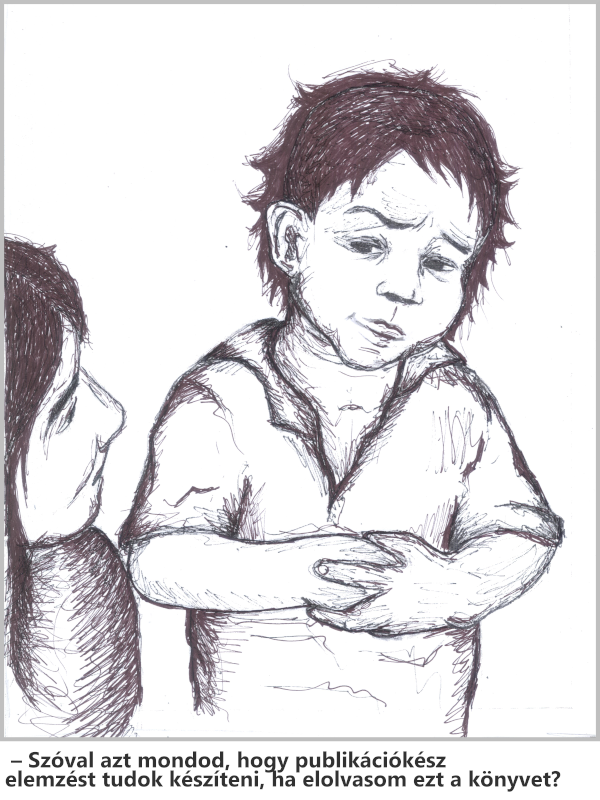
\includegraphics[width=0.7\linewidth]{images/ch_01_small} \end{center}



\hypertarget{Itt-kezdodik-1-szint}{%
\section{Elindulás}\label{Itt-kezdodik-1-szint}}

\begin{rmdlevel1}
Ebben a fejezetben:

\begin{itemize}
\tightlist
\item
  bemutatunk egy konkrét adatelemzési példát,
\item
  áttekintjük a könyv tartalmát,
\item
  lehetőséget adunk az előzetes R ismeretek felmérésére,
\item
  és segítünk a megfelelő fejezet kiválasztására a folytatáshoz.
\end{itemize}
\end{rmdlevel1}

Könyvünk elsődleges célja az R bemutatása kezdő felhasználók számára, de minden bizonnyal azok is találni fognak hasznos részeket, akik már rendelkeznek R ismeretekkel. Bevezetést nyújtunk az R által lefedett három nagy terület mindegyikébe: az adatkezelésbe, a grafikus megjelenítésbe és az adatelemzésbe is. A leírtak megértéséhez a statisztikai alapismereteken túl semmilyen előzetes tudás nem szükséges.

Most egy konkrét adatelemzési példa segítségével bemutatjuk, hogy mit nyújt e könyv az Olvasó számára. A bevezető példa megoldása során az előismeretekkel rendelkező Olvasó a saját R tudását is felmérheti, és ezzel egyben segítséget kaphat a tudásához és céljaihoz legjobban illeszkedő fejezet kiválasztására, amellyel tovább folytathatja az olvasást.

\textbf{Bevezető példa: Két tanítási módszer összehasonlítása}\\
Egy 2020-as kutatásunkban \citep{Csapo2020} 7. osztályos tanulóknak Excel ismereteket oktattunk két különböző megközelítésben. Az egyik csoportban hagyományos, míg a másikban modern (Sprego) tanítási módszert használtunk. A tanulási időszak az Excel ismeretek felmérésével zárult. Az összegyűjtött adatok az \texttt{excel\_2020.xlsx} állományban állnak rendelkezésre.\\
Nézzük az adatelemzés lépéseit és egyben könyvünk felépítését!

\textbf{2. fejezet: Mi az R?}\\
A bevezető példa megoldását R-ben fogjuk elvégezni (és nem más eszközben, mint például az SPSS, jamovi, JASP, SAS stb.). Érdemes tehát ismerni az R céljait és lehetőségeit, jó ha van egy összképünk a használt statisztikai programcsomagról. Ezt az áttekintést nyújtja 2 fejezet.

\textbf{3. fejezet: Az R telepítése.}\\
Adatelemzésünk konkrét lépéseinek elvégzéséhez telepített \emph{Alap R} és \emph{RStudio} szükséges. Ha ezek nem állnak rendelkezésre, vagy még nem is találkoztunk ezekkel az eszközökkel, akkor a 3. fejezet nekünk szól.

\textbf{4. fejezet: Munka az R-ben.}\\
Az adatelemzés végrehajtásához az \emph{RStudio}-t ajánljuk, és azon belül pedig a projektek használatát szorgalmazzuk. A 4. fejezetben megismerjük az \emph{RStudio} legalapvetőbb funkcióit, a parancsállományok létrehozását és futtatását.

A fenti előzmények után elkezdhetjük a bevezető példa megoldását:

\begin{enumerate}
\def\labelenumi{\arabic{enumi}.}
\tightlist
\item
  indítsuk el az \emph{RStudio}-t,
\item
  hozzunk létre egy új projektet,
\item
  hozzunk létre egy új RMarkdown állományt,
\item
  helyezzük el a lentebb szereplő R parancsokat az RMarkdown állomány egyes csonkjaiban.
\end{enumerate}

\textbf{5. fejezet: Az R nyelv.}\\
Az R parancsok létrehozásának vannak szabályai, amelyeket a munka során be kell tartanunk. Ismernünk kell jó néhány függvényt, és általában el kell tudnunk igazodni az R nyelvben. Az 5. fejezet ezért kulcsfontosságú, tanulmányozzuk alaposan, és lehetőleg minden kitűzött feladatát oldjuk meg.

\textbf{6. fejezet: Beolvasás}\\
Minden adatelemzés első lépése az adatállomány beolvasása. Adataink változatos formában állhatnak rendelkezésre, a 6. fejezetben ezek beolvasására kapunk receptet.

A bevezető példa megoldásához az RMarkdown állomány egyik csonkját bővítsük a lenti sorokkal.

\begin{Shaded}
\begin{Highlighting}[]
\CommentTok{\# install.packages("rio")                         \# rio csomag telepítése}
\FunctionTok{library}\NormalTok{(rio)                                      }\CommentTok{\# rio csomag betöltése}
\NormalTok{felmeres }\OtherTok{\textless{}{-}} \FunctionTok{import}\NormalTok{(}\AttributeTok{file =} \StringTok{"adat/excel\_2020.xlsx"}\NormalTok{) }\CommentTok{\# beolvasás}
\end{Highlighting}
\end{Shaded}

\textbf{7. fejezet: Adatkezelés}\\
A statisztikai elemzés elkezdése előtt számos adatkezelési tevékenységre lehet szükség. Ezt a sokszor rendkívül időigényes folyamatot a 7. fejezetben részletezzük.

A bevezető példa megoldásához az RMarkdown állomány egyik csonkját bővítsük a lenti sorokkal. Az adatkezelés legtöbbször a beolvasott állomány \emph{jellemzőinek lekérésével} kezdődik.

\begin{Shaded}
\begin{Highlighting}[]
\FunctionTok{str}\NormalTok{(felmeres)              }\CommentTok{\# a dataframe szerkezete}
\FunctionTok{names}\NormalTok{(felmeres)            }\CommentTok{\# változónevek  }
\FunctionTok{unique}\NormalTok{(felmeres}\SpecialCharTok{$}\NormalTok{modszer)   }\CommentTok{\# különböző értékek}
\end{Highlighting}
\end{Shaded}

A karakteres vagy numerikus vektorok faktorrá konvertálása az egyik leggyakoribb előkészítő parancs.

\begin{Shaded}
\begin{Highlighting}[]
\NormalTok{felmeres}\SpecialCharTok{$}\NormalTok{modszer }\OtherTok{\textless{}{-}} \FunctionTok{factor}\NormalTok{(felmeres}\SpecialCharTok{$}\NormalTok{modszer)}
\end{Highlighting}
\end{Shaded}

A táblázatok és ábrák megfelelő megjelenéséhez, végezzük el a \emph{faktorszintek sorrendbe állítását}.

\begin{Shaded}
\begin{Highlighting}[]
\NormalTok{felmeres}\SpecialCharTok{$}\NormalTok{modszer }\OtherTok{\textless{}{-}} \FunctionTok{factor}\NormalTok{(felmeres}\SpecialCharTok{$}\NormalTok{modszer, }\AttributeTok{levels=}\FunctionTok{c}\NormalTok{(}\StringTok{"modern"}\NormalTok{, }\StringTok{"hagyományos"}\NormalTok{))}
\end{Highlighting}
\end{Shaded}

\textbf{8. fejezet: Mutatók és táblázatok.}\\
Ha az adatainkat már megfelelő formába hoztuk, akkor továbbléphetünk az elemzés felé. A 8. fejezet a leíró statisztikai elemzésekből a mutatók és a táblázatok létrehozását mutatja be.

Most a felmérés eredményeinek statisztikai mutatóit íratjuk ki a két tanítási módszert használó csoportban.

\begin{Shaded}
\begin{Highlighting}[]
\CommentTok{\# install.packages("psych") \# psych csomag telepítése}
\NormalTok{psych}\SpecialCharTok{::}\FunctionTok{describeBy}\NormalTok{(}\AttributeTok{x =}\NormalTok{ felmeres}\SpecialCharTok{$}\NormalTok{eredmeny, }\AttributeTok{group =}\NormalTok{ felmeres}\SpecialCharTok{$}\NormalTok{modszer,}
                  \AttributeTok{mat=}\NormalTok{T, }\AttributeTok{fast=}\NormalTok{T, }\AttributeTok{digits =} \DecValTok{2}\NormalTok{)}
\CommentTok{\#\textgreater{}     item      group1 vars  n mean   sd  min  max range   se}
\CommentTok{\#\textgreater{} X11    1      modern    1 13 0.65 0.20 0.33 0.95  0.63 0.05}
\CommentTok{\#\textgreater{} X12    2 hagyományos    1 13 0.38 0.13 0.08 0.55  0.47 0.04}
\end{Highlighting}
\end{Shaded}

\textbf{9. fejezet: Grafika.}\\
A grafikus megjelenítés is a leíró statisztikai elemzés része. A 9. fejezetben részletesebben olvashatunk a publikációkész ábrák létrehozásáról.

Most a numerikus változók esetén használt egyik elterjedt ábrázolási formát, a dobozdiagramot használjuk két tanítási csoport eredményének grafikus összehasonlítására.

\begin{Shaded}
\begin{Highlighting}[]
\FunctionTok{library}\NormalTok{(ggplot2)}
\FunctionTok{ggplot}\NormalTok{(}\AttributeTok{data =}\NormalTok{ felmeres, }\AttributeTok{mapping =} \FunctionTok{aes}\NormalTok{(}\AttributeTok{x=}\NormalTok{modszer, }\AttributeTok{y=}\NormalTok{eredmeny)) }\SpecialCharTok{+} \FunctionTok{geom\_boxplot}\NormalTok{()}
\end{Highlighting}
\end{Shaded}

\begin{center}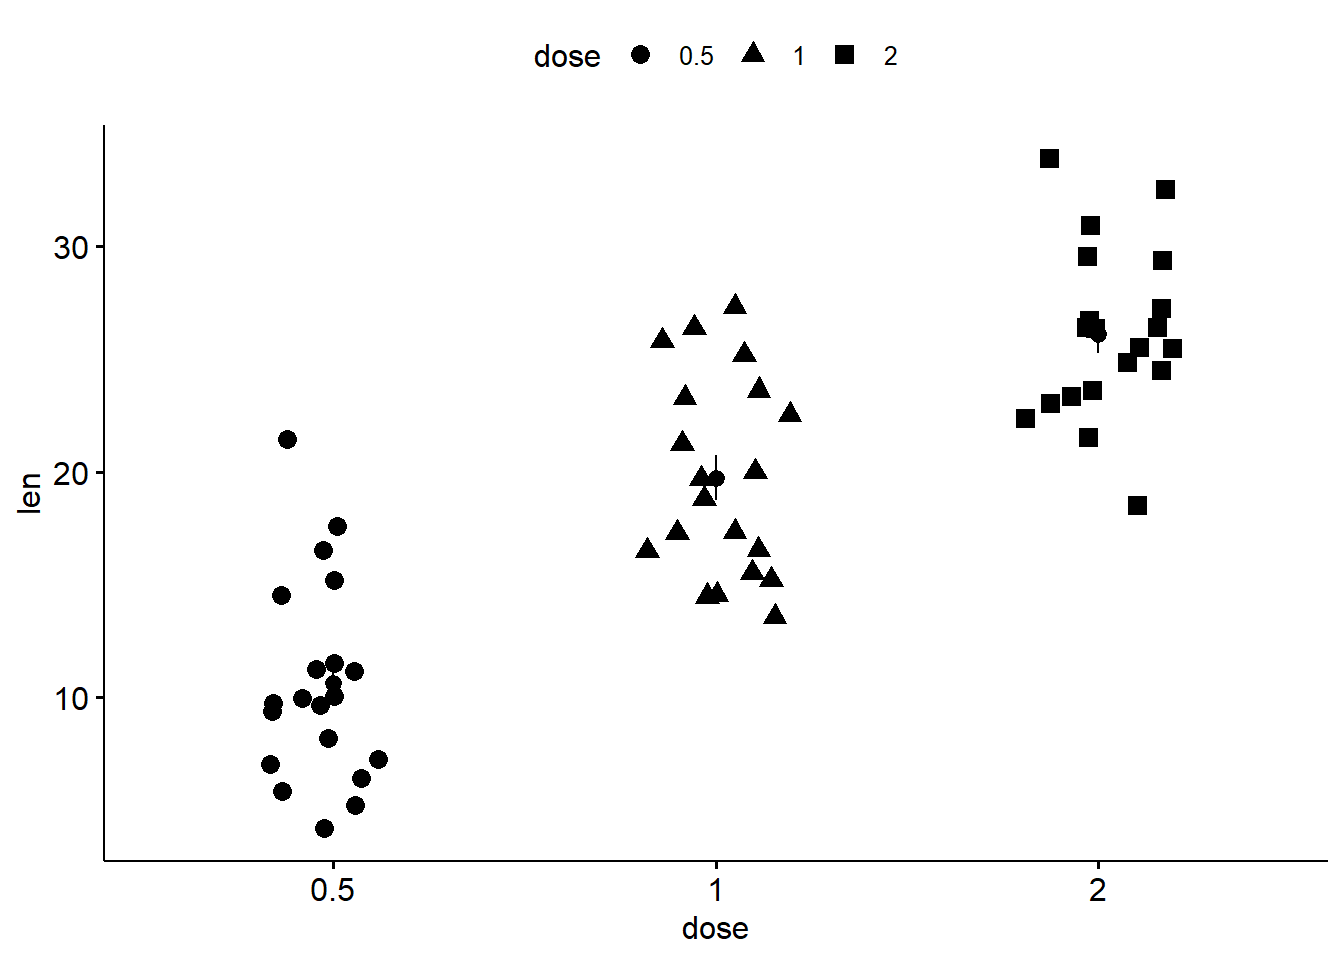
\includegraphics[width=0.7\linewidth]{01-Itt-kezdodik_files/figure-latex/unnamed-chunk-9-1} \end{center}

\textbf{10. fejezet: Hipotézisvizsgálatok.}\\
A statisztikai hipotézisvizsgálat minden adatelemzés központi része, a gyűjtött adatokból a populációra nézve következtetést vonhatunk le. A 10. fejezetben a leggyakoribb egyváltozós elemzéseket mutatjuk be.

Most Mann-Whitney-próbát hajtunk végre a két tanítási módszer eredményességének összehasonlítására.

\begin{Shaded}
\begin{Highlighting}[]
\FunctionTok{wilcox.test}\NormalTok{(eredmeny}\SpecialCharTok{\textasciitilde{}}\NormalTok{modszer, }\AttributeTok{data=}\NormalTok{felmeres)}
\CommentTok{\#\textgreater{} }
\CommentTok{\#\textgreater{}  Wilcoxon rank sum exact test}
\CommentTok{\#\textgreater{} }
\CommentTok{\#\textgreater{} data:  eredmeny by modszer}
\CommentTok{\#\textgreater{} W = 145, p{-}value = 0.001}
\CommentTok{\#\textgreater{} alternative hypothesis: true location shift is not equal to 0}
\end{Highlighting}
\end{Shaded}

\textbf{11. fejezet: Publikálás.}\\
Az adatelemzési folyamat utolsó lépése, az elemzés eredményének publikációkész formába öntése. A 11. fejezetben megismerjük azokat a legegyszerűbb folyamatokat, amelyekkel többnyire formanyelvtől függetlenül, publikációkész eredményközlést végezhetünk.

Most a bevezető példában kapott eredmények publikálását végezzük el. A korábban használt \texttt{psych::describeBy()} függvény hívását úgy módosítjuk, hogy az bármely formanyelven (PDF, HTML, Docx) megfelelő eredményt adjon. Ehhez mindössze egészítsük ki a következő sorokkal a leíró statisztikai elemzést, majd a \emph{Knit} nyomógomb segítségével fordítsuk le az RMarkdown állományt. A leíró statisztikai mutatók máris táblázatos, könnyen áttekinthető formában jelennek meg.

\begin{Shaded}
\begin{Highlighting}[]
\FunctionTok{options}\NormalTok{(}\AttributeTok{OutDec =} \StringTok{","}\NormalTok{)  }\CommentTok{\# a tizedesjel beállítása}
\NormalTok{st }\OtherTok{\textless{}{-}}\NormalTok{ psych}\SpecialCharTok{::}\FunctionTok{describeBy}\NormalTok{(}\AttributeTok{x =}\NormalTok{ felmeres}\SpecialCharTok{$}\NormalTok{eredmeny, }\AttributeTok{group =}\NormalTok{ felmeres}\SpecialCharTok{$}\NormalTok{modszer, }
                        \AttributeTok{mat=}\NormalTok{T, }\AttributeTok{fast=}\NormalTok{T, }\AttributeTok{digits =} \DecValTok{2}\NormalTok{)}
\NormalTok{knitr}\SpecialCharTok{::}\FunctionTok{kable}\NormalTok{(st[}\SpecialCharTok{{-}}\DecValTok{1}\NormalTok{], }\AttributeTok{align =} \FunctionTok{c}\NormalTok{(}\StringTok{"c"}\NormalTok{, }\StringTok{"c"}\NormalTok{), }\AttributeTok{row.names =}\NormalTok{ F)}
\end{Highlighting}
\end{Shaded}

\begin{tabular}{c|c|c|c|c|c|c|c|c}
\hline
group1 & vars & n & mean & sd & min & max & range & se\\
\hline
modern & 1 & 13 & 0,65 & 0,20 & 0,33 & 0,95 & 0,63 & 0,05\\
\hline
hagyományos & 1 & 13 & 0,38 & 0,13 & 0,08 & 0,55 & 0,47 & 0,04\\
\hline
\end{tabular}

Publikációnk szerves része a magyarázó ábra. A korábban rajzolt dobozdiagramunkat csinosítsuk ki a következő sorok R csonkba helyezésével. A \texttt{ggsave()} függvény a háttértárra rögzítésről is gondoskodik.

\begin{Shaded}
\begin{Highlighting}[]
\FunctionTok{library}\NormalTok{(ggplot2)}
\NormalTok{p1 }\OtherTok{\textless{}{-}} \FunctionTok{ggplot}\NormalTok{(}\AttributeTok{data =}\NormalTok{ felmeres, }\AttributeTok{mapping =} \FunctionTok{aes}\NormalTok{(}\AttributeTok{x=}\NormalTok{modszer, }\AttributeTok{y=}\NormalTok{eredmeny)) }\SpecialCharTok{+} 
  \FunctionTok{geom\_boxplot}\NormalTok{() }\SpecialCharTok{+} 
  \FunctionTok{labs}\NormalTok{(}\AttributeTok{x=}\ConstantTok{NULL}\NormalTok{, }\AttributeTok{y=}\StringTok{"Eredmény (\%)"}\NormalTok{, }
       \AttributeTok{title=}\StringTok{"7. osztályos tanulók Excel eredménye"}\NormalTok{, }
       \AttributeTok{subtitle =} \StringTok{"Két tanulási módszer összehasonlítása"}\NormalTok{) }\SpecialCharTok{+} 
  \FunctionTok{scale\_y\_continuous}\NormalTok{(}\AttributeTok{labels =}\NormalTok{ scales}\SpecialCharTok{::}\NormalTok{percent) }\SpecialCharTok{+} \FunctionTok{theme\_bw}\NormalTok{()}
\FunctionTok{ggsave}\NormalTok{(}\AttributeTok{filename =} \StringTok{"output/kep/dd.png"}\NormalTok{, }\AttributeTok{plot =}\NormalTok{ p1)}
\NormalTok{p1}
\end{Highlighting}
\end{Shaded}

\begin{center}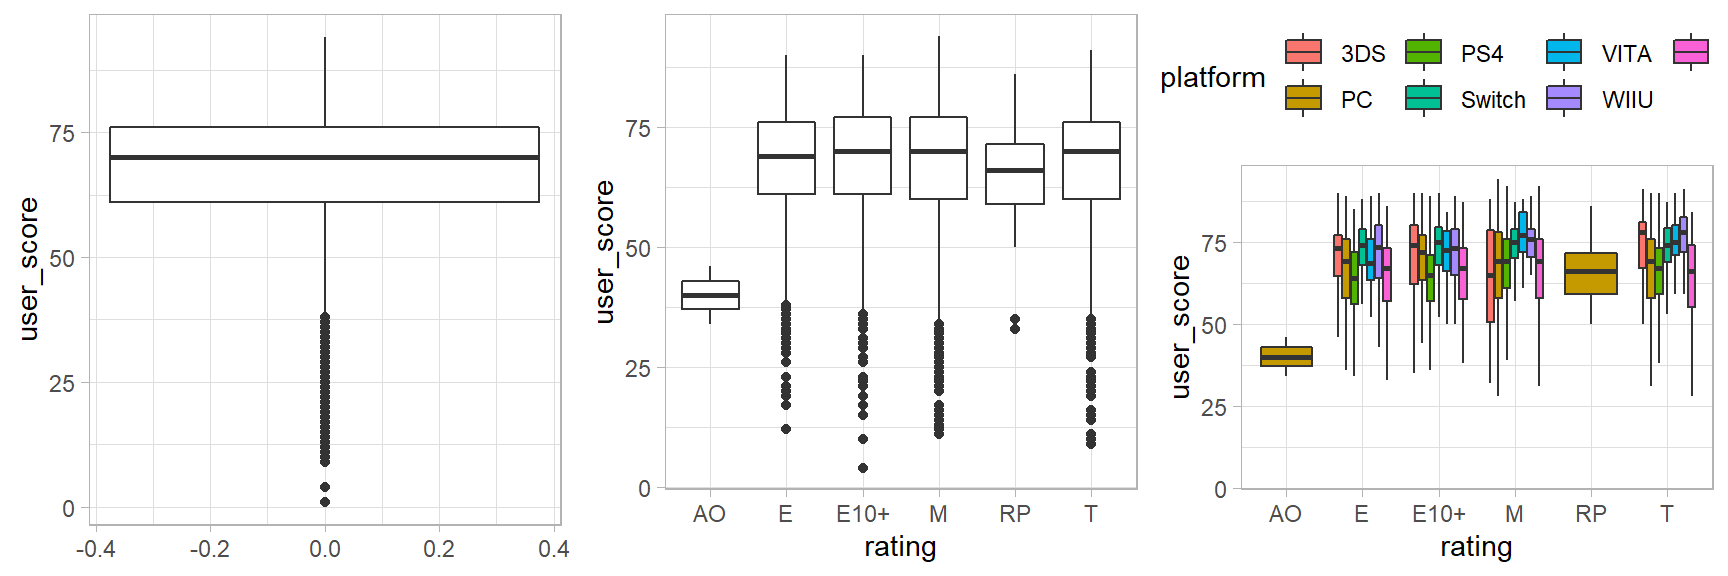
\includegraphics[width=0.7\linewidth]{01-Itt-kezdodik_files/figure-latex/unnamed-chunk-12-1} \end{center}

A bevezető példa megoldásához természetesen a hipotézisvizsgálat szöveges értékelés is hozzátartozik, de ezt most az alfejezet végén szereplő egyik kitűzött feladatra halasztjuk. A hangsúly a könyv vázlatos tartalomjegyzékének bemutatásán volt, részletesebb, de felsorolásszerű tartalomjegyzéket a következő két alfejezetben találunk.

\hypertarget{itt-kezdodik-1-summary}{%
\subsection{Összefoglalás}\label{itt-kezdodik-1-summary}}

\begin{rmdsummary}
Ebben az alfejezetben egy adatelemzési példát oldottunk meg, melynek
segítségével illusztrálni tudtuk a további fejezetek tartalmát. A 2.
fejezetben áttekintést adunk az R-ről, a 3.-ban az \emph{Alap R} és
\emph{RStudio} telepítését, a 4.-ben az \emph{RStudio} használatát
mutatjuk be. Az 5. fejezetben kellő részletességgel ismertetjük az R
nyelvet. A további fejezetekben az adatelemzés szokásos lépéseit vesszük
sorra, a 6. fejezetben a beolvasást, a 7. fejezetben az adatok
előkészítését, a 8. és 9. fejezetben a leíró statisztikai műveleteket
mutatjuk be. A 10. fejezet az egyváltozós hipotézisvizsgálatoké, az
utolsó, 11. fejezet az eredmények publikálását foglalja össze.
\end{rmdsummary}

\hypertarget{itt-kezdodik-1-exercise}{%
\subsection{Feladatok}\label{itt-kezdodik-1-exercise}}

\begin{rmdexercise}
\begin{enumerate}
\def\labelenumi{\arabic{enumi}.}
\tightlist
\item
  Milyen online vagy nyomtat könyvek segítik az R elsajátítását?
  Próbáljuk összegyűjteni a magyar nyelvű könyveket is!
\item
  Térképezzük fel az online videókurzusokat is az R tanulásához!
\item
  A bevezető példa (\emph{Két tanítási módszer összehasonlítása})
  megoldásában a hipotézisvizsgálat alapján adjunk szöveges értékelést!
\end{enumerate}
\end{rmdexercise}

\hypertarget{a-kuxf6nyv-feluxe9puxedtuxe9se}{%
\section{A könyv felépítése}\label{a-kuxf6nyv-feluxe9puxedtuxe9se}}

\begin{rmdlevel2}
Ebben a fejezetben:

\begin{itemize}
\tightlist
\item
  bemutatjuk a könyv részletes felépítését,
\item
  ezzel tovább segítjük a választást a folytatáshoz.
\end{itemize}
\end{rmdlevel2}

A könyv 11 fejezetből áll, és fejezetenként 3 vagy több alfejezetből. Most röviden bemutatjuk az egyes alfejezetek tartalmát.

\begingroup\fontsize{10}{11}\selectfont

\begin{longtable}[]{@{}
  >{\raggedright\arraybackslash}p{(\columnwidth - 2\tabcolsep) * \real{0.3438}}
  >{\raggedright\arraybackslash}p{(\columnwidth - 2\tabcolsep) * \real{0.6562}}@{}}
\toprule
\begin{minipage}[b]{\linewidth}\raggedright
Fejezet/alfejezet
\end{minipage} & \begin{minipage}[b]{\linewidth}\raggedright
Leírás
\end{minipage} \\
\midrule
\endhead
\textbf{1. Itt kezdődik} & \\
1.1. Elindulás & A könyv fejezeteinek bemutatása egy konkrét adatelemzésen keresztül \\
1.2. A könyv felépítése & Jelen alfejezet, amelyben a könyv egyes alfejezeteit mutatjuk be röviden \\
1.3. Próbák listája & A könyvben szereplő egyváltozós statisztikai eljárások listája \\
& \\
\textbf{2. Mi az R?} & \\
2.1. Az R bemutatása & A parancssoros R jellemzői, az R nyelv, az \emph{Alap R} és a csomag fogalma \\
2.2. A modern R & Megtanuljuk a \emph{Tidyverse R} fogalmát, megtudjuk mi a modern R \\
2.3. Múlt és jelen & Az R rövid története, alapelvek az R tanulásához, és az R alaptudás elemei \\
& \\
\textbf{3. Az R telepítése} & \\
3.1. Az Alap R és az RStudio telepítése & Megismerjük az \emph{Alap R} és az \emph{RStudio} telepítését \\
3.2. A Tidyverse R telepítése & A \textbf{tidyverse} csomag(gyűjtemény) telepítése \\
3.3. Az R frissítése & Az \emph{Alap R}, az \emph{RStudio} és a csomagok frissítésének módszerei \\
& \\
\textbf{4. Munka az R-ben} & \\
4.1. Az RStudio használata & Az \emph{RStudio} jellemzői és felépítése, a projektek használata \\
4.2. Segítség az R használatához & Segítségkérési lehetőségek az R-ben, a beépített súgó használata \\
4.3. Az Alap R használata & Az \emph{Alap R} konzolja, az \emph{RGui}, az \emph{R Commander} és a kötegelt üzemmód \\
& \\
\textbf{5. Az R nyelv} & \\
5.1 Adatobjektumok & Az objektumok fogalma és létrehozásuk, egyszerű kifejezések \\
5.2 Függvények & A függvény fogalma, a függvényhívás módja, a kifejezés teljes fogalma \\
5.3 Adatszerkezetek & Az R egyszerű és összetett adatszerkezetei, létrehozásuk és indexelésük \\
5.4 További adatszerkezetek és függvények & A dátum, tömb, táblázat és tibble adatszerkezetek kezelése \\
5.5 Objektumok és típusok & Az R objektum-orientált lehetőségei \\
\textbf{6. Beolvasás} & \\
6.1 Excel, SPSS és RDS állományok & A \emph{rio} csomag lehetőségei \\
6.2 Tidyverse beolvasás & A \emph{tidyverse} csomag lehetőségei \\
6.3 Tagolt szöveges állományok & A hagyományos R lehetőségei \\
& \\
\textbf{7. Adatmanipuláció} & \\
& \\
\textbf{8. Mutatók és táblázatok} & \\
& \\
\textbf{9. Grafika} & \\
& \\
\textbf{10. Hipotézisvizsgálatok} & \\
& \\
\textbf{11. Publikáció} & \\
\bottomrule
\end{longtable}

\endgroup{}

\hypertarget{itt-kezdodik-2-summary}{%
\subsection{Összefoglalás}\label{itt-kezdodik-2-summary}}

\begin{rmdsummary}
Ebben a részben röviden bemutattuk a könyv összes alfejezetét. A
későbbiekben térképként használhatja az Olvasó az itt ismertetett
táblázatot.
\end{rmdsummary}

\hypertarget{itt-kezdodik-2-exercise}{%
\subsection{Feladatok}\label{itt-kezdodik-2-exercise}}

\begin{rmdexercise}
\begin{enumerate}
\def\labelenumi{\arabic{enumi}.}
\tightlist
\item
  Az adatfeldolgozás 4 lépése a következő: (1) adatok beolvasása, (2) adatok előkészítése elemzésre, (3) adatok elemzése és (4) az eredmények publikálása. A könyv mely fejezetei tartoznak az adatfeldolgozás fenti lépéseihez?
\item
  Az R-rel való munka általunk javasolt módja: \emph{RStudio}-ban, projektmódban, R vagy RMarkdown állományokat szerkesztünk és hajtunk végre. Mely fejezetekben találunk hasznos információkat az R ezen használatával kapcsolatban?
\end{enumerate}
\end{rmdexercise}

\hypertarget{pruxf3buxe1k-listuxe1ja}{%
\section{Próbák listája}\label{pruxf3buxe1k-listuxe1ja}}

\begin{rmdlevel3}
Ebben a fejezetben:

\begin{itemize}
\tightlist
\item
  áttekintést adunk az egy- és kétváltozós hipotézisvizsgálatokról.
\end{itemize}
\end{rmdlevel3}

A 10. fejezetben bemutatjuk az egy- és kétváltozós hipotézisvizsgálatok végrehajtását. Ebben a fejezetben felsoroljuk a legfontosabb próbákat, összesen öt táblázatban soroljuk fel őket:

\begin{itemize}
\tightlist
\item
  egy mintát vizsgáló próbák (\ref{tab:egyminta1}. táblázat),
\item
  páros mintát vizsgáló próbák (\ref{tab:parosminta1}. táblázat),
\item
  két független mintát vizsgáló próbák (\ref{tab:ketminta1}. táblázat),
\item
  több összetartozó mintát vizsgáló próbák (\ref{tab:tobbosszeminta1}. táblázat),
\item
  több független mintát vizsgáló próbák (\ref{tab:tobbminta1}. táblázat).
\end{itemize}

A táblázatokban megadjuk, hogy a vizsgálatnak mi a célja, vagyis a populációbeli változó(k) melyik paraméterére vonatkoznak a próbák, a várható értékre, a mediánra, a varianciára vagy a valószínűségre. A 10. fejezetben foglalkozunk az eloszlásvizsgálatok közül a normalitást ellenőrző próbákkal is, így a \ref{tab:egyminta1}. táblázat ezeket is számba veszi.

\begin{longtable}[]{@{}
  >{\raggedright\arraybackslash}p{(\columnwidth - 4\tabcolsep) * \real{0.2088}}
  >{\raggedright\arraybackslash}p{(\columnwidth - 4\tabcolsep) * \real{0.4835}}
  >{\raggedright\arraybackslash}p{(\columnwidth - 4\tabcolsep) * \real{0.3077}}@{}}
\caption{\label{tab:egyminta1} Egy minta vizsgálata}\tabularnewline
\toprule
\begin{minipage}[b]{\linewidth}\raggedright
Cél
\end{minipage} & \begin{minipage}[b]{\linewidth}\raggedright
Próba neve
\end{minipage} & \begin{minipage}[b]{\linewidth}\raggedright
R függvény
\end{minipage} \\
\midrule
\endfirsthead
\toprule
\begin{minipage}[b]{\linewidth}\raggedright
Cél
\end{minipage} & \begin{minipage}[b]{\linewidth}\raggedright
Próba neve
\end{minipage} & \begin{minipage}[b]{\linewidth}\raggedright
R függvény
\end{minipage} \\
\midrule
\endhead
várható érték & egymintás u-próba & \texttt{BSDA::z.test()} \\
& egymintás t-próba & \texttt{t.test()} \\
medián & előjel-próba & \texttt{BSDA::SIGN.test()} \\
& Mood-féle medián-próba & \\
& egymintás Wilcoxon-próba & \texttt{wilcox.test()} \\
variancia & khí-négyzet próba & \texttt{chisq.test()} \\
valószínűség & khí-négyzet próba & \texttt{chisq.test()} \\
normalitás & Shapiro-Wilk próba & \texttt{shapiro.test()} \\
& Kolmogorov-Szmirnov próba & \texttt{DescTools:LillieTest()} \\
\bottomrule
\end{longtable}

\begin{longtable}[]{@{}
  >{\raggedright\arraybackslash}p{(\columnwidth - 4\tabcolsep) * \real{0.2088}}
  >{\raggedright\arraybackslash}p{(\columnwidth - 4\tabcolsep) * \real{0.4835}}
  >{\raggedright\arraybackslash}p{(\columnwidth - 4\tabcolsep) * \real{0.3077}}@{}}
\caption{\label{tab:parosminta1} Páros minta vizsgálata}\tabularnewline
\toprule
\begin{minipage}[b]{\linewidth}\raggedright
Cél
\end{minipage} & \begin{minipage}[b]{\linewidth}\raggedright
Próba neve
\end{minipage} & \begin{minipage}[b]{\linewidth}\raggedright
R függvény
\end{minipage} \\
\midrule
\endfirsthead
\toprule
\begin{minipage}[b]{\linewidth}\raggedright
Cél
\end{minipage} & \begin{minipage}[b]{\linewidth}\raggedright
Próba neve
\end{minipage} & \begin{minipage}[b]{\linewidth}\raggedright
R függvény
\end{minipage} \\
\midrule
\endhead
várható érték & páros t-próba & \texttt{t.test(paired=T)} \\
medián & páros előjel-próba & \texttt{BSDA::SIGN.test()} \\
& páros Wilcoxon-próba & \texttt{wilcox.test(paired=T)} \\
variancia & & \texttt{var.test()} \\
valószínűség & McNemar-próba & \texttt{mcnemar.test()} \\
& Cohran-Q próba & \texttt{mcnemar.test()} \\
\bottomrule
\end{longtable}

\begin{longtable}[]{@{}
  >{\raggedright\arraybackslash}p{(\columnwidth - 4\tabcolsep) * \real{0.2088}}
  >{\raggedright\arraybackslash}p{(\columnwidth - 4\tabcolsep) * \real{0.4835}}
  >{\raggedright\arraybackslash}p{(\columnwidth - 4\tabcolsep) * \real{0.3077}}@{}}
\caption{\label{tab:ketminta1} Két független minta vizsgálata}\tabularnewline
\toprule
\begin{minipage}[b]{\linewidth}\raggedright
Cél
\end{minipage} & \begin{minipage}[b]{\linewidth}\raggedright
Próba neve
\end{minipage} & \begin{minipage}[b]{\linewidth}\raggedright
R függvény
\end{minipage} \\
\midrule
\endfirsthead
\toprule
\begin{minipage}[b]{\linewidth}\raggedright
Cél
\end{minipage} & \begin{minipage}[b]{\linewidth}\raggedright
Próba neve
\end{minipage} & \begin{minipage}[b]{\linewidth}\raggedright
R függvény
\end{minipage} \\
\midrule
\endhead
várható érték & kétmintás u-próba & \texttt{BSDA::z.test()} \\
& kétmintás t-próba & \texttt{t.test()} \\
& Welch-féle d-próba & \texttt{t.test(var.equal=F)} \\
medián & Mann--Whitney-próba & \texttt{wilcox.test()} \\
variancia & F-próba & \texttt{var.test()} \\
valószínűség & khí-négyzet próba & \texttt{chisq.test()} \\
& Fisher-féle egzakt próba & \texttt{fisher.test()} \\
\bottomrule
\end{longtable}

\begin{longtable}[]{@{}
  >{\raggedright\arraybackslash}p{(\columnwidth - 4\tabcolsep) * \real{0.2639}}
  >{\raggedright\arraybackslash}p{(\columnwidth - 4\tabcolsep) * \real{0.4167}}
  >{\raggedright\arraybackslash}p{(\columnwidth - 4\tabcolsep) * \real{0.2917}}@{}}
\caption{\label{tab:tobbosszeminta1} Több összetartozó minta vizsgálata}\tabularnewline
\toprule
\begin{minipage}[b]{\linewidth}\raggedright
Cél
\end{minipage} & \begin{minipage}[b]{\linewidth}\raggedright
Próba neve
\end{minipage} & \begin{minipage}[b]{\linewidth}\raggedright
R függvény
\end{minipage} \\
\midrule
\endfirsthead
\toprule
\begin{minipage}[b]{\linewidth}\raggedright
Cél
\end{minipage} & \begin{minipage}[b]{\linewidth}\raggedright
Próba neve
\end{minipage} & \begin{minipage}[b]{\linewidth}\raggedright
R függvény
\end{minipage} \\
\midrule
\endhead
várható érték & \begin{minipage}[t]{\linewidth}\raggedright
egyszempontos összetartozó\\
mintás varianciaelemzés\strut
\end{minipage} & \texttt{ez::ezANOVA()} \\
medián & Friedman-próba & \texttt{friedman.test()} \\
\bottomrule
\end{longtable}

\begin{longtable}[]{@{}
  >{\raggedright\arraybackslash}p{(\columnwidth - 4\tabcolsep) * \real{0.2088}}
  >{\raggedright\arraybackslash}p{(\columnwidth - 4\tabcolsep) * \real{0.4835}}
  >{\raggedright\arraybackslash}p{(\columnwidth - 4\tabcolsep) * \real{0.3077}}@{}}
\caption{\label{tab:tobbminta1} Több független minta vizsgálata}\tabularnewline
\toprule
\begin{minipage}[b]{\linewidth}\raggedright
Cél
\end{minipage} & \begin{minipage}[b]{\linewidth}\raggedright
Próba neve
\end{minipage} & \begin{minipage}[b]{\linewidth}\raggedright
R függvény
\end{minipage} \\
\midrule
\endfirsthead
\toprule
\begin{minipage}[b]{\linewidth}\raggedright
Cél
\end{minipage} & \begin{minipage}[b]{\linewidth}\raggedright
Próba neve
\end{minipage} & \begin{minipage}[b]{\linewidth}\raggedright
R függvény
\end{minipage} \\
\midrule
\endhead
várható érték & egyszempontos varianciaelemzés & \texttt{aov()} \\
& Welch-féle egyszempontos varianciaelemzés & \texttt{oneway.test(var.equal=F)} \\
medián & Kruskal--Wallis-próba & \texttt{kruskal.test()} \\
variancia & Levene-próba & \texttt{DescTools::LeveneTest()} \\
& Bartlett-próba & \texttt{bartlett.test()} \\
\bottomrule
\end{longtable}

\hypertarget{itt-kezdodik-3-summary}{%
\subsection{Összefoglalás}\label{itt-kezdodik-3-summary}}

\begin{rmdsummary}
Ebben a részben rövid áttekintést adtunk a könyv 10. fejezetében sorra
kerülő statisztikai próbákról. Megneveztük a próbákat, R parancsokkal
szemléltettük használatukat, valamint jeleztük a céljukat. A táblázatok
áttekintésével képet kaphatunk arról, hogy a későbbiekben milyen jellegű
statisztikai következtetéseket tudunk levonni az R használatával.
\end{rmdsummary}

\hypertarget{itt-kezdodik-3-exercise}{%
\subsection{Feladatok}\label{itt-kezdodik-3-exercise}}

\begin{rmdexercise}
\begin{enumerate}
\def\labelenumi{\arabic{enumi}.}
\tightlist
\item
  Minden statisztikai próba esetében négy dolgot érdemes tudni: (1) a statisztikai próba neve, (2) null- és ellenhipotézise, (3) alkalmazási feltételei, és (4) a próba végrehajtásának módja valamely statisztikai programcsomagban. A 10. fejezetben a statisztikai próbák végrehajtását természetesen R-beli eszközökkel mutatjuk be. Ismerjük a fenti táblázatokban megnevezett próbák null- és ellenhipotézisét, valamint az alkalmazási feltételeit? Próbáljuk ezeket felidézni! Hol találunk ezekről információt?
\item
  Mely próbák maradtak ki ebből a könyvből? Hol találunk ezek R-beli végrehajtására példát?
\end{enumerate}
\end{rmdexercise}

\hypertarget{mi-az-r}{%
\chapter{Mi az R?}\label{mi-az-r}}

\begin{center}
\includegraphics[width=0.6\linewidth]{images/ch_02_small} \end{center}

\hypertarget{az-r-bemutatuxe1sa}{%
\section{Az R bemutatása}\label{az-r-bemutatuxe1sa}}

\begin{rmdlevel1}
Ebben a fejezetben:

\begin{itemize}
\tightlist
\item
  megismerjük az R jellemzőit,
\item
  megtudjuk, hogy melyek a parancssoros interfész előnyei,
\item
  megismerjük az \emph{Alap R} fogalmát,
\item
  körülhatároljuk az R nyelv, az \emph{Alap R} és a csomag fogalmát.
\end{itemize}
\end{rmdlevel1}

\hypertarget{az-r-jellemzux151i}{%
\subsection{Az R jellemzői}\label{az-r-jellemzux151i}}

Az R egy magas szintű programozási nyelv és környezet, amelynek legfontosabb felhasználása az adatelemzés és az ahhoz kapcsolódó grafikus megjelenítés. Három alapvető jellemzője kiemeli a többi statisztikai programcsomag közül: (1) az R ingyenesen telepíthető és használható; (2) az R nyílt forrású, így bárki hozzájárulhat az R fejlesztéséhez, azaz létrehozhat új \emph{csomag}okat, és ezzel kiegészítheti az R tudását; és (3) az R felhasználók rendkívül aktív és befogadó online közösséget alkotnak, szinte minden felmerülő kérdésünkre azonnal választ kaphatunk.

Álljon itt egy bővített lista azokról a jellemzőkről, amelyek vonzóvá tehetik számunkra az R statisztikai programcsomagot.

\begin{itemize}
\tightlist
\item
  Az R szabad szoftver, bárki ingyenesen letöltheti és használhatja. Ez egyfelől megkönnyíti az oktatási intézmények, tanszékek és oktatók munkáját, hiszen nincs szükség a kereskedelmi programok licenceléséből adódó pénzügyi vagy más természetű nehézségek kezelésére. Másrészt a hallgatók a statisztika kurzusok során tanultakat otthon vagy később a munkájukban is felhasználhatják.
\item
  Az R platform-független, azaz Windows, Linux és macOS környezetben is használható. Nem kell lemondanunk a kedvenc operációs rendszerünkről, ha az R-t szeretnénk használni.
\item
  Az R nemcsak egy statisztikai programcsomag önmagában, hanem egy teljes értékű programozási nyelv.
\item
  Az R statisztikai módszerek szinte végtelen választékát kínálja. A R-ben felhasználható statisztikai eljárásokat statisztikusok fejlesztik folyamatosan és csomagok formájában teszik elérhetővé. Valószínű, hogy egy új statisztikai módszer leghamarabb az R-ben válik elérhetővé.
\item
  Az R rendkívül gazdag grafikus lehetőségekkel rendelkezik.
\item
  A statisztikai szakirodalomban és az egyetemi oktatók körében egyre elterjedtebb az R mint közös (statisztikai program)nyelv használata. Ha valamilyen statisztikai problémára keressük a megoldást, vagy csak konzultálunk egy statisztikussal, az R ismerete (akár csak olvasási szinten) rendkívüli előnyt jelenthet.
\item
  Az R igen jól dokumentált, a beépített súgón kívül számos könyv és leírás érhető el.
\item
  Az R parancssoros interfésszel rendelkezik, amely számos előnnyel jár. Egyrészt a szkript állományok létrehozása és végrehajtása a statisztikai elemzések megismételhetőségét biztosítják, másrészt ez az oktatók és a hallgatók könnyebb kommunikációját is lehetővé teszi.
\item
  Az R az adatelemzés eredményének sokszínű publikálását is biztosítja. Az \href{https://rmarkdown.rstudio.com/}{RMarkdown} formanyelv segítségével HTML, PDF és Word dokumentumot, illetve prezentációs diákat vagy akár kész cikkeket hozhatunk létre. A \href{http://shiny.rstudio.com/}{Shiny} csomag interaktív Webes alkalmazások építését teszi lehetővé.
\item
  Mára az R használata szinte egyet jelent az ingyenesen elérhető \href{https://www.rstudio.com/}{\emph{RStudio}} használatával, amely egy kényelmes integrált fejlesztői környezetet biztosít a parancsállományok létrehozásához.
\end{itemize}

Érdemes bepillantani az R árnyékosabb oldalába is. Az R egyik gyengesége, hogy nagy adatbázisok kezeléséhez erős hardverre van szüksége, de a legtöbb felhasználás során ez semmilyen problémát nem okoz. A másik gyengeség, hogy az R elsajátításához nem kevés idő és kitartás szükséges. Jelen könyv éppen ezt a folyamatot kívánja megkönnyíteni és lerövidíteni.

\hypertarget{a-r-parancssoros}{%
\subsection{A R parancssoros}\label{a-r-parancssoros}}

Az R alapvető használata során parancsokat gépelünk be és hajtunk végre. Ez lényegesen eltér a ma megszokott felhasználói programok világától, ahol egy grafikus felhasználói felületen egérrel vagy az ujjunkkal mutogatjuk el a kívánt tevékenységet. Az R egészen más megközelítést vall, használata a kezdeti lépésektől nagyfokú figyelmet és pontosságot követel. Parancsokban kell gondolkodnunk, ám ezt végig áthatja a \emph{tudom mit csinálok} elv, így némi idő elteltével érezni fogjuk, hogy az R megszelídül, már nem köt bele minden szavunkba, egyre több dologra tudjuk rávenni, és végül egy rendkívül értékes társsá válik. Jelen könyv ezen az úton szeretné végigvezetni az Olvasót.

Már a tanulás elején szeretnénk tisztázni, hogy az R elsajátításához nem szükséges programozói alaptudás. Az R felhasználók többsége egyáltalán nem programozó, és a mindennapi adatelemző munka sem igényli az R nyelv programozói fokú ismeretét. Természetesen, ha rendelkezünk ilyen irányú előtanulmányokkal a tanulási folyamat néhány szakasza lerövidíthető, de könyvünk elsősorban azok számra íródott, akik programozási nyelvekkel korábban nem találkoztak, és nem is vágynak az R ilyen mélységű ismeretére. Az R nyelv elsajátítása során bevezetjük azokat az egyszerű fogalmakat, amelyeket nem nélkülözhetők az adatelemzés során, azonban az R programozásához más szakkönyveket javaslunk olvasásra.

\hypertarget{mi-valuxf3juxe1ban-az-r}{%
\subsection{Mi valójában az R?}\label{mi-valuxf3juxe1ban-az-r}}

Az R nyelv fejlesztője az \href{https://www.r-project.org/contributors.html}{R Core Team}. Az R nyelv egy rendkívül népszerű szkriptnyelv, több millióan használják világszerte. Elsősorban adatelemzésre, adatmodellezésre és grafikus megjelenítésre, vagyis arra, amit ma adattudományok (data science) alatt értünk. Azonban az R nyelv önmagában nem szoftver, hanem egy rendkívül rugalmas szkriptnyelv, amely például előírja, hogy milyen szintaktikai szabályok mentén fogalmazhatjuk meg az utasításainkat. Ahhoz, hogy az R nyelvet használni tudjuk, vagyis, hogy a számítógép valóban végre is hajtsa a szintaktikailag helyes utasításainkat, szükség van egy szoftveres környezetre, egy olyan futtató rendszerre, amely a kódunkat értelmezi és végrehajtja.

\begin{figure}

{\centering \href{}{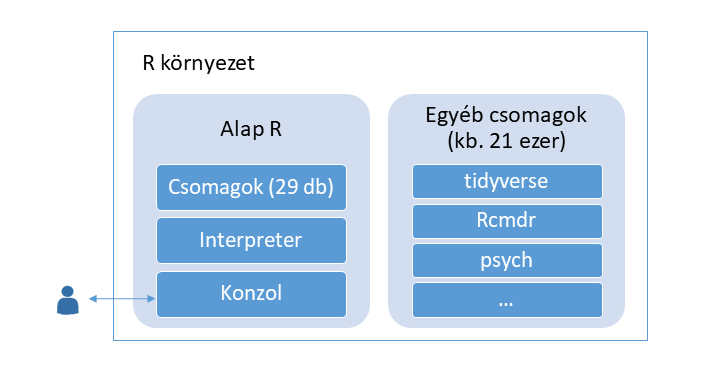
\includegraphics[width=0.85\linewidth]{images/alapr_kornyezet} }

}

\caption{Az R környezet: Alap R és az egyéb csomagok}\label{fig:ralapkorny-01}
\end{figure}

Az R környezet három fő összetevőt tartalmaz (\ref{fig:ralapkorny-01}. ábra): (1) egy \emph{konzol}t, ahová a parancsainkat begépelhetjük; (2) a parancsok végrehajtásáért felelős \emph{R interpreter}t; (3) a \emph{csomagokok}at. A konzol és az interpreter biztosítja az R nyelven írt parancsok tényleges végrehajtását. Így tudunk adatokat beolvasni, átlagot számolni, varianciaelemzést futtatni, vagy publikációkész ábrákat létrehozni. A csomagok adatokat és függvényeket tartalmaznak, például a \textbf{MASS} csomag 88 adatobjektumot és 78 függvényt tartalmaz. A függvények valamilyen tevékenységet hajtanak végre, és valójában ezeket a csomag-függvényeket használjuk fel a konzolban, ha \emph{bármilyen tevékenységet} szeretnénk végrehajtani (például adatokat beolvasni, átlagot számolni stb.). A könyv írásának időpontjában kb. 21 ezer csomag volt érhető el az R-hez. Csomagok 3 csoportját különböztetjük meg: \emph{standard csomagok} (14 db), \emph{ajánlott csomagok} (15 db) és \emph{egyéb csomagok} (kb. 21 ezer db). A standard csomagok fejlesztője az R Core Team. A standard csomagok: \textbf{base}, \textbf{compiler}, \textbf{datasets}, \textbf{grDevices}, \textbf{graphics}, \textbf{grid}, \textbf{methods}, \textbf{parallel}, \textbf{splines}, \textbf{stats}, \textbf{stats4}, \textbf{tcltk}, \textbf{tools}, \textbf{utils}. Az ajánlott csomagok: \textbf{KernSmooth}, \textbf{MASS}, \textbf{Matrix}, \textbf{boot}, \textbf{class}, \textbf{cluster}, \textbf{codetools}, \textbf{foreign}, \textbf{lattice}, \textbf{mgcv}, \textbf{nlme}, \textbf{nnet}, \textbf{rpart}, \textbf{spatial}, \textbf{survival}. Az ajánlott csomagok közül a \textbf{foreign} és az \textbf{nlme} fejlesztője az R Core Team, a többit más felhasználók fejlesztették, például a már említett \textbf{MASS} csomag fejlesztője Brian Ripley. Csomagot bárki szabadon fejleszthet és terjeszthet, az \emph{egyéb csomagok} csoportját akár mi is gyarapíthatjuk.

A R környezet már igazi szoftver, terjesztésének koordinálását az \href{https://www.r-project.org/foundation/}{R Foundation} végzi a \href{https://cran.r-project.org/mirrors.html}{CRAN} infrastruktúráján keresztül. Ez biztosítja, hogy számítógépünkre telepíthessük az R környezetet. Ezt a CRAN-ról elérhető R futtatási környezetet \emph{Alap R}-nek nevezzük. Fő komponensei a már említett konzol a parancsok begépelésére, az R értelmező a begépelt parancsok végrehajtására és a csomagok közül a standard és ajánlott csomagok. Az \emph{Alap R} telepítése után már tudunk R parancsokat végrehajtani, és nagyon sok adatelemzési probléma megoldására nyílik módunk, sőt azt mondhatjuk, hogy tetszőleges problémát megoldhatunk kisebb-nagyobb erőfeszítéssel, mert az R egy teljes értékű nyelv. Azonban sokszor érdemesebb az \emph{egyéb csomagok} közül választani, hiszen könnyen elképzelhető, hogy a számtalan csomag között találunk olyat, amely segítségünkre lehet speciális feladataink megoldása során. Valószínű, hogy létezik olyan csomag és benne olyan függvény, amely adatkezelési, adatelemzési, grafikai vagy publikálási feladatunkat jelentősen megkönnyíti. Az \emph{egyéb csomagok} csoportjába tartozó csomagok forrása több tárhely is lehet, ezek közül legjelentősebb az R Foundation által karbantartott CRAN (18407 csomaggal), a Bioconductor (2140 csomaggal) és a GitHub.

Az R tehát egyszerre több dolgot jelent. Az R egyrészt egy magas szintű programozási nyelv, hamarosan megtanuljuk, hogyan írjunk ezen a nyelven értelmes utasításokat. Másrészt a nyelv körüli környezetet is jelenti, amely magába foglalja a konzolt, a parancsaink értelmezésért felelős R interpretert, valamint azokat a csomagokat, amelyekkel az R tudása kiegészíthető.

\hypertarget{mi-az-r-1-summary}{%
\subsection{Összefoglalás}\label{mi-az-r-1-summary}}

\begin{rmdsummary}
Minden statisztikai programcsomag, így az R is, alapvetően a
számításigényes statisztikai eljárások kézi végrehajtásától kímél meg
minket. Az R nagyon gazdag adatmanipulációs és grafikus funkciókban is,
támogatja a reprodukálható adatelemzés végrehajtását. Az R ingyenes,
többplatformos és egyik legfontosabb jellemzője, hogy parancsok útján
bírhatjuk működésre. Az \emph{Alap R} biztosítja a konzolt a parancsok
begépelésére, az R interpretert a parancsok tényleges végrehajtására, és
jó néhány csomagba szervezett eljárást az adatelemzési feladatok
elvégzéséhez. Az \emph{Alap R} mindössze néhány tucat csomagot
tartalmaz, a \emph{standard csomagokat} és az \emph{ajánlott
csomagokat}, de több tízezer további csomaggal bővíthetjük az R tudását.
Az adatelemzési munka során egy R környezet vesz minket körül, amely az
R nyelven megírt parancsok értelmezésére és végrehajtására képes
\emph{Alap R}-ből, és az ún. \emph{egyéb csomagokból} áll.
\end{rmdsummary}

\hypertarget{mi-az-r-1-exercise}{%
\subsection{Feladatok}\label{mi-az-r-1-exercise}}

\begin{rmdexercise}
\begin{enumerate}
\def\labelenumi{\arabic{enumi}.}
\tightlist
\item
  Keressünk weboldalakat, amelyek az R előnyeit és hátrányait listázzák!
\item
  Keressük meg, hogy az R optimális futtatásához, milyen hardver követelmények szükségesek!
\item
  Nézzünk utána, hogy ma kb. hány csomag érhető el az R-hez? Keressünk ábrát, amely bemutatja, hogy az évek során hány csomag volt elérhető az R-hez?
\item
  Hol áll az R népszerűsége a többi programozási nyelvhez, illetve statisztikai programcsomaghoz képest?
\item
  Milyen ingyenesen elérhető, grafikus felhasználói felülettel rendelkező statisztikai programcsomagok építenek az R-re?
\item
  Említettük, hogy az adatelmezési munka nem igényli az R programozói fokú ismeretét, de soroljunk fel néhány könyvet, amelyből az R programozása is megtanulható!
\end{enumerate}
\end{rmdexercise}

\hypertarget{a-modern-r}{%
\section{A modern R}\label{a-modern-r}}

\begin{rmdlevel2}
Ebben a fejezetben:

\begin{itemize}
\tightlist
\item
  megismerjük a \emph{Tidyverse R} fogalmát,
\item
  megtudjuk mit értünk modern R alatt.
\end{itemize}
\end{rmdlevel2}

A 2014-es év az R nyelv életében meghatározó változást hozott. Egyrészt megjelent a \textbf{magrittr} csomagban a pipe operátor (\texttt{\%\textgreater{}\%}), amellyel olvashatóbb kódok írására nyílt lehetőség\footnote{Más programozási nyelvekben az ``objektum'' helyett a ``változó'' elnevezést használják, de a változó fogalma már foglalt a statisztikában, így szerencsésebb a memóriában tárolt adatokra objektumként hivatkozni.}, másrészt a pipe operátorra alapozva Hadley Wickham bemutatta a \textbf{dplyr} és \textbf{tidyr} csomagokat. Ezzel az R funkcionális\footnote{Az R egy nem túl fiatal, a funkcionális programnyelvekhez hasonlóan építkező programozási nyelv, vagyis egy probléma megoldása tipikusan sokszorosan egymásba ágyazott függvényhívások segítségével történik. Ez sok-sok nyitó és záró kerek zárójellel jár együtt, így a parancsaink áttekintése és karbantartása sokszor nehézségekbe ütközik. Ezt kiküszöbölendő az R-ben előszeretettel használnak procedurális eszközöket (például \texttt{for} ciklusokat), de a kód olvashatóságát és karbantartását igazán ez sem könnyíti meg.} oldalát úgy erősítették meg\footnote{További értékadás operátorok a \texttt{-\textgreater{}}, \texttt{\textless{}\textless{}-}, \texttt{-\textgreater{}\textgreater{}} és a \texttt{=}. Ezeket nem használjuk ebben a könyvben.}, hogy a sokszoros egymásba ágyazás során kiküszöbölték a kerek zárójelek írásának problémáját. Az ebben a szellemben készült csomagok listája bővült az idők folyamán, és a \emph{Tidyverse} nevet kapta ez a csomaggyűjtemény. Jelenleg a következő csomagok alkotják: \textbf{ggplot2}, \textbf{purrr}, \textbf{tibble}, \textbf{dplyr}, \textbf{tidyr}, \textbf{stringr}, \textbf{readr} és \textbf{forcats}. Ezek a csomagok nem egyszerűen új funkciókkal ruházzák fel az \emph{Alap R} tudását, mint általában az \emph{egyéb csomagok}. A \emph{Tidyverse} csomagjai konzisztens módon együttműködnek, és egy új megközelítést hoznak az adatelemzési folyamatok végrehajtásában és a kódok írásában. Rövidebb idő alatt hozhatunk létre könnyebben karbantartható kódokat, és a műveleteink végrehajtása is rendszerint gyorsabb. Amikor ebben a megközelítésben hozzuk létre és hajtjuk végre utasításainkat, akkor azt mondjuk hogy a \emph{Tidyverse R}-t használjuk. A \emph{Tidyverse R} nem helyettesíti az \emph{Alap R}-t, és csak bizonyos feladatokra használható. Lássunk tisztán, amit elvégezhetünk \emph{Tidyverse R}-ben, azt az \emph{Alap R}-ben is meg tudnánk tenni, de valószínűleg több gépeléssel, lassabb és rosszabbul karbantartható kóddal.

Eddig láttuk, hogy az R használatához szükséges az \emph{Alap R} telepítése, majd a speciális problémánknak megfelelően kiegészíthetjük az R tudását úgy, hogy telepítünk egyet vagy többet az \emph{egyéb csomagok} kategóriájából. Választhatjuk akár a \emph{Tidyverse} csomagjait is telepítésre, ugyanis így lehetőségünk nyílik a \emph{Tidyverse R} használatára. Utasításaink megfogalmazásának ma ez a legmodernebb módja.

A modern R alatt lényegében azokat a funkciókat értjük, amelyek a \href{https://www.tidyverse.org/}{\emph{Tidyverse}} gyűjteményben található csomagokhoz kötődnek. Ezekkel a csomagokkal, gyorsabb, olvashatóbb és könnyebben karbantartható kódokat hozhatunk létre. A \emph{Tidyverse} használata tehát erősen javasolt, de ebben a könyvben a ``hagyományos'', \emph{Tidyverse R} előtti lehetőségeket is bemutatjuk.

\hypertarget{mi-az-r-2-summary}{%
\subsection{Összefoglalás}\label{mi-az-r-2-summary}}

\begin{rmdsummary}
A \emph{Tidyverse R} egy csomaggyűjtemény az \emph{egyéb csomagok}
csoportjából, amely újabb szemléletű R parancsok írására ad lehetőséget.
Az így készült kódjaink rendszerint gyorsabban futnak és könnyebben
karbantarthatók. A modern R a \emph{Tidyverse R} csomagjaival
kiegészített \emph{Alap R}, de legfőképp egy új lehetőség parancsaink
megfogalmazására.
\end{rmdsummary}

\hypertarget{mi-az-r-2-exercise}{%
\subsection{Feladatok}\label{mi-az-r-2-exercise}}

\begin{rmdexercise}
\begin{enumerate}
\def\labelenumi{\arabic{enumi}.}
\tightlist
\item
  Ki Hadley Wickham?
\item
  Mikor történt az egyik legjobb dolog az R-rel?
\end{enumerate}
\end{rmdexercise}

\hypertarget{muxfalt-uxe9s-jelen}{%
\section{Múlt és jelen}\label{muxfalt-uxe9s-jelen}}

\begin{rmdlevel3}
Ebben a fejezetben:

\begin{itemize}
\tightlist
\item
  megismerjük az R rövid történetét és annak szereplőit,
\item
  majd egy szubjektív listával segítjük az R tanulását,
\item
  illetve megismerjük az R alaptudás elemeit.
\end{itemize}
\end{rmdlevel3}

\hypertarget{szereplux151k-uxe9s-fogalmak}{%
\subsection{Szereplők és fogalmak}\label{szereplux151k-uxe9s-fogalmak}}

Érdemes néhány szereplőt és fogalmat tisztázni az R világán belül. Az R nyelvet 1992-ben kezdte fejleszteni \href{https://www.stat.auckland.ac.nz/~ihaka/}{Ross Ihaka} és \href{https://www.linkedin.com/in/robert-gentleman-06845098/}{Robert Gentleman}, 1997-től pedig egy nagyobb csapat, az \href{https://www.r-project.org/contributors.html}{R Development Core Team} vezeti a fejlesztést (rövidebben \emph{R Core Team}). Ettől az évtől az R hivatalosan a GNU projekt része. Az \emph{R Core Team} tagjai 2002-ben létrehozták a \href{https://www.r-project.org/foundation/}{The R Foundation for Statistical Computing} (rövidebben \emph{The R Foundation}) közhasznú, nonprofit szervezetet, amelynek célja (1) az R folyamatos fejlesztésének biztosítása, és ehhez kapcsolódóan a nyílt forráskódú számítógépes statisztikai innovációk támogatása, (2) az R fejlesztői közösség (\emph{R Core Team}) hivatalos hangjaként a felhasználók, intézmények és üzleti vállalkozások számára a kommunikáció biztosítása, és (3) az R program és dokumentációk szerzői jogainak kezelése. A szervezet rendszeresen konferenciákat, találkozókat szervez, referált folyóiratot, kézikönyveket és technikai leírásokat ad ki, valamint fenntart egy számítógépes infrastruktúrát (ez a CRAN, amely levelező listákat, FTP- és Webszervereket üzemeltet). Az R Foundation hivatalos oldala -- egyben az R hivatalos oldala -- a \href{https://www.r-project.org/}{\emph{https://www.r-project.org/}}. Az R Foundation (és más önkéntesek) által üzemeltetett számítógépes hálózat neve a CRAN (Comprehensive R Archive Network), amely szabad hozzáférést nyújt az R legfrissebb verziójához, az R kiterjesztéseihez (a csomagokhoz) és a részletes dokumentációkhoz. A CRAN fő számítógépe Ausztriában található \href{https://CRAN.R-project.org/}{\emph{https://CRAN.R-project.org/}}, azonban nagyon sok naponta frissülő \href{https://cran.r-project.org/mirrors.html}{tükörszerver} érhető el világszerte.

\hypertarget{alapelvek}{%
\subsection{Alapelvek}\label{alapelvek}}

Az R elsődleges célja, hasonlóan más statisztikai programcsomagokhoz, a statisztikai adatelemzés, amelyet négy lépésre bonthatunk:

\begin{enumerate}
\def\labelenumi{\arabic{enumi}.}
\tightlist
\item
  adatok beolvasása,
\item
  adatok előkészítése elemzésre,
\item
  adatelemzés,
\item
  eredmények publikálása.
\end{enumerate}

Az R mára a fenti 4 tevékenység elvégzését teljes körűen támogatja. A könyv célja ezek bemutatása. Mielőtt elkezdjük ezt az izgalmas utat -- az R tanulmányozását -- néhány alapelvet szeretnék megemlíteni, ami segíthet minket az utazásunk során:

\begin{itemize}
\tightlist
\item
  \emph{Magabiztosság} - Az R nagyon nagy, így a teljes megismerése nem lehet célunk. Mindig lesz valaki, aki az R egyik vagy másik részét jobban, vagy kevésbé ismeri nálunk. Ez természetes, ezen soha ne csodálkozzunk. Az eltérő ismeretek azonban az R speciális területeire vonatkoznak, az \emph{R alaptudás} (\ref{Ralaptudas}. fejezet) minden R-ben jártas felhasználó számára közös. E könyv célja ennek az alaptudásnak az átadása, melynek birtokában már kellő magabiztossággal vághatunk neki az R azon részeinek elsajátításába, amelyek az éppen elénk kerülő speciális feladat megoldásához szükségesek. Hisszük, hogy e könyv elolvasásával, mind az R alaptudás, mind a kellő magabiztosság elérhetővé válik számunkra.
\item
  \emph{Gyakorlás} - Az R alaptudásának megszerzése némi időbe telik, ez tagadhatatlan. A motiváció megtartásához viszonylag jól kell éreznünk magunkat a tanulás és a gyakorlás során. A könyvben ezért minden fejezet végén találunk megoldandó feladatokat, amelyek között szórakoztató, érdekes és kihívást jelentő gyakorlatok is szerepelnek.
\item
  \emph{Svájci bicska} - A R nagyon sokféle statisztikai és nem-statisztikai probléma megoldására képes, sőt ugyanarra a problémára nagyon sok különböző eszközt kínál. Ha elsőre nem a legszebb, legoptimálisabb megoldás jut az eszünkbe, ne csüggedjünk, ez a legtöbb esetben nem jelent gondot. Azon se csodálkozzunk, ha korábban megoldott problémánkra idővel újabb és újabb megoldási lehetőségeket találunk.
\end{itemize}

\hypertarget{Ralaptudas}{%
\subsection{Az R alaptudás}\label{Ralaptudas}}

Melyek az R-ben való munkavégzéshez nélkülözhetetlen alapismeretek? Meggyőződésünk, ha a lentebb felsorolt témakörökkel tisztában vagyunk, akkor már magabiztos R tudással rendelkezünk, és bármilyen további R témakör könnyen elsajátítható lesz. Ezekre az ismeretekre úgy gondolhatunk, mint egy ablakra, amelyen keresztül az R szinte végtelen lehetőségeinek tárháza nyílik meg előttünk. Később visszatérhetünk ehhez a listához, és ellenőrizhetjük, hány elemet tudunk már kipipálni.

\textbf{Az R alaptudás elemei:}

\begin{itemize}
\tightlist
\item
  Az R környezet alapszintű ismerete

  \begin{itemize}
  \tightlist
  \item[$\square$]
    az \emph{Alap R}, az \emph{RStudio} és a csomagok telepítése
  \item[$\square$]
    projektek használata és R parancsok futtatása az \emph{RStudio}-ban
  \end{itemize}
\item
  Az R nyelv alapszintű ismerete

  \begin{itemize}
  \tightlist
  \item[$\square$]
    konstansok írása
  \item[$\square$]
    objektumok kezelése
  \item[$\square$]
    egyszerű adattípusok
  \item[$\square$]
    alapvető operátorok
  \item[$\square$]
    kifejezés fogalma
  \item[$\square$]
    a függvényhívás lehetőségei
  \item[$\square$]
    összetett adattípusok,
  \item[$\square$]
    a vektoraritmetika szabályai
  \end{itemize}
\item
  Az alapvető függvények ismerete

  \begin{itemize}
  \tightlist
  \item[$\square$]
    csomagkezelő függvények
  \item[$\square$]
    a munkaterület függvényei
  \item[$\square$]
    matematikai függvények
  \item[$\square$]
    input/output függvények
  \item[$\square$]
    indexelés, szűrés, rendezés
  \item[$\square$]
    információ kérés az objektumokról
  \item[$\square$]
    egyszerű típuskonverzió
  \item[$\square$]
    transzformáció
  \item[$\square$]
    ismétlő és összesítő függvények
  \item[$\square$]
    a hagyományos grafika néhány eleme
  \item[$\square$]
    a \textbf{ggplot2} alapszintű ismerete
  \end{itemize}
\item
  Egyéb ismeretek

  \begin{itemize}
  \tightlist
  \item[$\square$]
    szövegszerkesztési és állománykezelési ismeretek
  \item[$\square$]
    a tagolt szöveges állomány fogalma
  \item[$\square$]
    reprodukálható kutatás az RMarkdown segítségével
  \end{itemize}
\end{itemize}

\hypertarget{mi-az-r-3-summary}{%
\subsection{Összefoglalás}\label{mi-az-r-3-summary}}

\begin{rmdsummary}
Az R fejlesztését Ross Ihaka és Robert Gentleman kezdte, majd 1997-től
egy nagyobb csapat, az \emph{R Development Core Team} vezeti a
fejlesztést. Az \emph{R Core Team} tagjai 2002-ben létrehozták a
\emph{The R Foundation for Statistical Computing} közhasznú, nonprofit
szervezetet, amelynek fő célja az R folyamatos fejlesztésének
biztosítása. A szervezet fenntart egy CRAN nevű számítógépes hálózatot,
amely szabad hozzáférést biztosít az R legfrissebb verziójához, a
csomagokhoz és a részletes dokumentációkhoz.\\
Az R alaptudás megszerzése elegendő magabiztosságot fog nyújtani az
adatelemzési munka során, azonban vegyük figyelembe, hogy ezt csak kellő
gyakorlással érhetjük el. Az R sokféle megoldást biztosít ugyanarra a
problémára, legyen az statisztikai vagy bármilyen más jellegű feladat.
\end{rmdsummary}

\hypertarget{mi-az-r-3-exercise}{%
\subsection{Feladatok}\label{mi-az-r-3-exercise}}

\begin{rmdexercise}
\begin{enumerate}
\def\labelenumi{\arabic{enumi}.}
\tightlist
\item
  Keressünk olyan statisztikai jellegű témaköröket, amelyekben az R segítségünkre lehet?
\item
  Keressünk olyan nem-statisztikai jellegű témaköröket, amelyekben az R segítségünkre lehet?
\item
  Nézzünk át néhány online elérhető R könyvet, és hasonlítsuk össze az R alaptudás egyes elemeivel! Melyek az átfedő részek, és hol vannak különbségek?
\item
  Melyek a fontosabb lépcsőfokok az R fejlődősében?
\end{enumerate}
\end{rmdexercise}

\hypertarget{az-r-telepitese}{%
\chapter{Az R telepítése}\label{az-r-telepitese}}

\begin{center}
\includegraphics[width=0.7\linewidth]{images/ch_03_small} \end{center}

\hypertarget{a-fux151-komponensek-telepuxedtuxe9se}{%
\section{A fő komponensek telepítése}\label{a-fux151-komponensek-telepuxedtuxe9se}}

\begin{rmdlevel1}
Ebben a fejezetben:

\begin{itemize}
\tightlist
\item
  megismerjük az \emph{Alap R}, az \emph{RStudio} és a csomagok
  telepítését.
\end{itemize}
\end{rmdlevel1}

A korábbi fejezetekben megismertük az R világának néhány fogalmát és szereplőjét. Tudjuk, hogy az R nyelv használatához megfelelő szoftveres környezetre van szükség, amely magába foglalja az \emph{Alap R}-t és az \emph{egyéb csomagok} kategóriájából esetlegesen telepített csomagokat is. Az R már ezen eszközök birtokában is teljes körűen használható, azonban egy újabb ingyenes eszköz, az \emph{RStudio}, kényelmessé és hatékonnyá teszi az adatelemzési munkát.

Könyvünk legfontosabb gondolata: \textbf{ma akkor tudjuk a legjobban kihasználni az R lehetőségeit, és ezzel egyidőben a legkényelmesebb módon elvégezni az adatelemzési feladatunkat, ha}

\begin{enumerate}
\def\labelenumi{\arabic{enumi}.}
\tightlist
\item
  \textbf{az \emph{Rstudio}-t használjuk,}
\item
  \textbf{projekt üzemmódban dolgozunk, és}
\item
  \textbf{RMarkdown állományokban rögzítjük az R parancsainkat.}
\end{enumerate}

Ezt a szemléletet következetesen képviseljük az egyes fejezetekben, és a későbbiekben részletesebben bemutatjuk, hogyan tudjuk mindezt megvalósítani (\ref{fig:alaprst02}. ábra).

\begin{figure}

{\centering \href{}{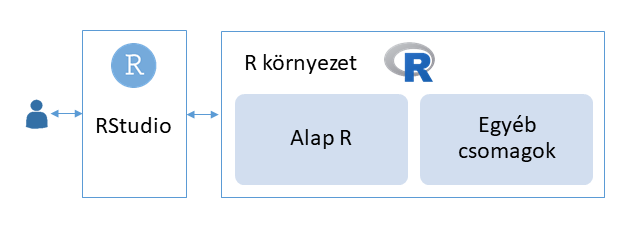
\includegraphics[width=0.85\linewidth]{images/alaprst02} }

}

\caption{Az R kényelmes használata}\label{fig:alaprst02}
\end{figure}

A R kényelmes használatához a legelső lépés a szoftveres környezet egyes elemeinek telepítése. Három fő komponens telepítésére lesz szükségünk:

\begin{enumerate}
\def\labelenumi{\arabic{enumi}.}
\tightlist
\item
  \emph{Alap R}, amely tartalmazza a konzolt, az R interpretert, illetve a \emph{standard csomagokat} és az \emph{ajánlott csomagokat},
\item
  \emph{RStudio}, amely egy új konzollal ``eltakarja'' az \emph{Alap R}-t, és kényelmesebb hozzáférést biztosít az \emph{Alap R} interpreteréhez és a csomagjaihoz.
\item
  Csomagok, amelyek az \emph{egyéb csomagok} nagy halmazából származnak, és telepítésükkel újabb és újabb képességekkel ruházzuk fel az \emph{Alap R}-t.
\end{enumerate}

\hypertarget{az-alap-r-telepitese}{%
\subsection{Az Alap R telepítése}\label{az-alap-r-telepitese}}

Az \emph{Alap R} telepítéséhez látogassunk el az R hivatalos letöltő oldalára: \emph{\url{https://cran.r-project.org/}}. Az operációs rendszerünknek megfelelő link kiválasztásával folytassuk a navigálást.

\begin{itemize}
\tightlist
\item
  A Windows felhasználók a \texttt{Download\ R\ for\ Windows} linken, majd a \texttt{base} linken kattintva jutnak el a telepítőprogram linkjéhez: \texttt{Download\ R\ X.X.X\ for\ Windows}. A sikeres letöltés után indítsuk el a telepítőt, és az alapértelmezetten felajánlott opciók nyugtázásával végezzük el a telepítést. A telepítést lehetőleg olyan Windows felhasználó alatt végezzük el, amelynek a neve sem ékezetes karaktert, sem szóközt, sem egyéb írásjelet nem tartalmaz.
\item
  A macOS felhasználók a \texttt{Download\ R\ for\ (Mac)\ OS\ X} linken kattintva jutnak a telepítőhöz: \texttt{R-X.X.X.pkg}. A letöltés után indítsuk el a telepítőt, és a \texttt{Next} gombok segítségével végezzük el a telepítést.
\item
  A Linux felhasználók az aktuális R verzió telepítéséhez a \texttt{Download\ R\ for\ Linux} linken keresztül jutnak el, ahol a megfelelő disztribúció (Debian, Redhat, Suse, Ubuntu) kiválasztása után konkrét információkat kapnak a telepítésről.
\end{itemize}

\hypertarget{az-rstudio-telepitese}{%
\subsection{Az RStudio telepítése}\label{az-rstudio-telepitese}}

Az \emph{RStudio} telepítéséhez az operációs rendszerünknek megfelelő telepítőt kell letöltenünk a \emph{\url{https://www.rstudio.com/products/rstudio/download/}} oldalról. Az \emph{RStudio Desktop (Open Source License)} változatra lesz szükségünk, töltsük le és telepítsük ezt a számítógépünkre. A telepítés során fogadjuk el az alapértelmezett opciókat. Az \emph{RStudio} automatikusan megtalálja és használja a korábban telepített \emph{Alap R} példányunkat, így a későbbiekben elegendő lesz az \emph{RStudio}-t használni, azon keresztül elérhetjük az \emph{Alap R} minden funkcióját (\ref{fig:alaprst02}. ábra).

\hypertarget{Csomagoktelepitese}{%
\subsection{Csomagok telepítése}\label{Csomagoktelepitese}}

A csomagok telepítésére az \emph{Alap R} vagy az \emph{RStudio} elindítása után van módunk. Érdemes a telepítéseket az \emph{RStudio}-ból végezni. A csomag fellelési helye alapján, három különböző tárhelyről mutatjuk be a csomagok telepítését. Látni fogjuk, hogy a csomagok telepítéséhez R parancsokat fogunk használni. Ha még nem vagyunk jártasak R parancsok futtatásban, akkor a \ref{AzRStudiohasznalata}. fejezet fellapozásával segítséget kaphatunk a lenti parancsok kipróbálásához, de úgy is eljárhatunk, hogy most kihagyjuk ennek a résznek az áttekintését, és később térünk vissza, amikor valóban felmerül az igény csomagok telepítésére.

Az R csomagok hivatalos helye a \href{https://cran.r-project.org/web/packages/}{CRAN (The Comprehensive R Archive Network)}. A CRAN számítógépei tárolják a nyílt forráskódú R nyelv és környezet különböző verzióinak kódjait és dokumentációit, így az összes R csomag forráskódját is. Egy bírálási folyamat után bármely felhasználó csomagja a CRAN-ból is elérhető lehet.

Az \emph{Alap R} vagy az \emph{RStudio} elindítása után az \texttt{install.packages()} függvénnyel tölthetünk le és telepíthetünk csomagot a CRAN-ról. Tetszőleges csomag telepítéséhez írjuk a csomag nevét idézőjelekben a függvény argumentumába:

\begin{Shaded}
\begin{Highlighting}[]
\NormalTok{install.packages("csomag\_neve")}
\end{Highlighting}
\end{Shaded}

A \textbf{psych} csomagot, amely a pszichológia kutatások adatainak elemzéséhez nyújt segítséget, például így telepíthetjük:

\begin{Shaded}
\begin{Highlighting}[]
\FunctionTok{install.packages}\NormalTok{(}\StringTok{"psych"}\NormalTok{)        }\CommentTok{\# psych csomag telepítése}
\end{Highlighting}
\end{Shaded}

A csomagok másik fontos forrása a \href{https://www.bioconductor.org/}{Bioconductor}, ahol alaposan tesztelt és igen jól dokumentált bioinformatikai témájú csomagokat találunk. Az innen elérhető csomagokat -- például most a \textbf{DESeq2} csomagot az RNS-szekvenálási elemzésekhez -- a következő parancsokkal telepíthetjük:

\begin{Shaded}
\begin{Highlighting}[]
\ControlFlowTok{if}\NormalTok{ (}\SpecialCharTok{!}\FunctionTok{requireNamespace}\NormalTok{(}\StringTok{"BiocManager"}\NormalTok{, }\AttributeTok{quietly =} \ConstantTok{TRUE}\NormalTok{))}
    \FunctionTok{install.packages}\NormalTok{(}\StringTok{"BiocManager"}\NormalTok{)}
\NormalTok{BiocManager}\SpecialCharTok{::}\FunctionTok{install}\NormalTok{(}\StringTok{"DESeq2"}\NormalTok{)}
\end{Highlighting}
\end{Shaded}

A csomagok harmadik fő forrása a GitHub. A felhasználók a saját fejlesztésű csomagjaikat rendszerint először a GitHub-on keresztül teszik elérhetővé. Ha ezeket a csomagokat szeretnénk kipróbálni, akkor a felhasználó és a csomag nevének birtokában a következő parancsot kell kiadnunk:

\begin{verbatim}
devtools::install_github("felhasznalo_neve/csomag_neve")
\end{verbatim}

Például a GitHub-ról telepíthető \textbf{emo} csomag segítségével hangulatjeleket szúrhatunk be az RMarkdown állományainkba. Ezzel a sorral telepíthetjük a csomagot:

\begin{Shaded}
\begin{Highlighting}[]
\NormalTok{devtools}\SpecialCharTok{::}\FunctionTok{install\_github}\NormalTok{(}\StringTok{"hadley/emo"}\NormalTok{)}
\end{Highlighting}
\end{Shaded}

Fontos tudnunk, hogy a csomagok telepítésére egy számítógépen egy adott R verzión belül csak egyszer van szükség. A telepítő parancsainkat azonban érdemes megőrizni, ugyanis egy új R verzióban könnyebben tudjuk így telepíteni a korábban használt csomagjainkat. Nagyon fontos, hogy a telepítő parancsok futtatása után, tegyük azokat megjegyzésbe, vagyis írjunk eléjük kettőskereszt (\texttt{\#}) karaktert (részletesebb információkat a megjegyzésekről a \ref{MegjegyzesazRben}. fejezetben olvashatunk). Ezzel tudjuk megvédeni ezeket a telepítő parancsokat az újbóli, véletlen, felesleges végrehajtástól. Ennek megfelelően a telepítő parancsainkat ilyen formában kell őriznünk:

\begin{Shaded}
\begin{Highlighting}[]
\CommentTok{\# install.packages("psych")        \# psych csomag telepítése}
\CommentTok{\# if (!requireNamespace("BiocManager", quietly = TRUE))}
\CommentTok{\#     install.packages("BiocManager")}
\CommentTok{\# BiocManager::install("DESeq2")}
\CommentTok{\# devtools::install\_github("hadley/emo")}
\end{Highlighting}
\end{Shaded}

Vegyük figyelembe, hogy egy csomag telepítése során más, egyéb csomagok telepítése automatikusan is megtörténhet, tehát egy helyett valójában több csomag is felkerülhet a gépünkre. Az is előfordulhat, hogy egy csomag telepítése csak akkor lesz sikeres, ha más csomagok frissítését engedélyezzük az adott csomag telepítése során. Végül előfordulhat olyan eset is, amikor egy csomag telepítése valamilyen oknál fogva meghiúsul. Erről minden esetben hibaüzenet tájékoztat minket, és ez szinte minden esetben jó kiindulásul szolgál a hibát okozó körülmény elhárításában. A legtöbbször egy másik csomag hiánya okozza a sikertelen telepítést, ezért olvassuk ki a hibaüzenetből a hiányolt csomag nevét, és először ennek a telepítését végezzük el. Nagyon ritka esetben az is előfordulhat, hogy egy csomag telepítését az \emph{RStudio} helyett az \emph{Alap R}-ben kell elvégeznünk.

\hypertarget{az-r-telepitese-1-summary}{%
\subsection{Összefoglalás}\label{az-r-telepitese-1-summary}}

\begin{rmdsummary}
Az R kényelmes használatához először telepítsük az operációs
rendszerünknek megfelelő \emph{Alap R}, majd az \emph{RStudio} legújabb
verzióját. Az R képességeit csomagok segítségével bővíthetjük, melyek
három különböző tárhelyről származhatnak. A legtöbb csomagot a CRAN-ről
telepíthetjük az \texttt{install.packages()} parancs használatával. A
Bioconductor-ról vagy a GitHub-ról származó csomagok telepítéséhez más
parancsokat kell használnunk.
\end{rmdsummary}

\hypertarget{az-r-telepitese-1-exercise}{%
\subsection{Feladatok}\label{az-r-telepitese-1-exercise}}

\begin{rmdexercise}
\begin{enumerate}
\def\labelenumi{\arabic{enumi}.}
\tightlist
\item
  Melyik az R legfrissebb változata, és milyen újdonságokat tartalmaz az előző változathoz képest?
\item
  Melyik az \emph{RStudio} legfrissebb változata, és milyen újdonságokat tartalmaz az előző változathoz képest?
\item
  Hogyan deríthető ki, hogy egy csomagban (például a \textbf{MASS}) csomagban, hány adatobjektum, és hány függvény található?
\end{enumerate}
\end{rmdexercise}

\hypertarget{a-tidyverse-r-telepuxedtuxe9se}{%
\section{A Tidyverse R telepítése}\label{a-tidyverse-r-telepuxedtuxe9se}}

\begin{rmdlevel2}
Ebben a fejezetben:

\begin{itemize}
\tightlist
\item
  megismerjük a \emph{Tidyverse R} telepítését.
\end{itemize}
\end{rmdlevel2}

A \emph{Tidyverse R} az R meglévő funkcióinak új szemléletű használatát jelenti. A modern R jelenleg egyet jelent a \emph{Tidyverse R}-rel, az ebben a szemléleteben készült parancsaink gyorsak, jól olvashatók és könnyen módosíthatók. A \emph{Tidyverse R} funkciói összesen több csomagba (például \textbf{ggplot2}, \textbf{purrr}, \textbf{tibble}, \textbf{dplyr}, \textbf{tidyr}, \textbf{stringr}, \textbf{readr} és \textbf{forcats}) vannak szétosztva, mindegyik csomag egy-egy témakört fed le. A fenti csomagok telepítése egyetlen gyűjtőcsomag a \textbf{tidyverse} nevű csomag telepítésével is elvégezhető:

\begin{Shaded}
\begin{Highlighting}[]
\FunctionTok{install.packages}\NormalTok{(}\StringTok{"tidyverse"}\NormalTok{) }\CommentTok{\# a Tidyverse R telepítése}
\end{Highlighting}
\end{Shaded}

A \emph{Tidyverse R} telepítését követően a csomagokban lévő függvények használatához a \emph{Tidyverse R} betöltésére is szükség van. Hívjuk meg a \texttt{library()} függvényt, amely ebben az esetben igen részletes tájékoztatást ad az újonnan elérhető csomagokról.

\begin{Shaded}
\begin{Highlighting}[]
\FunctionTok{library}\NormalTok{(tidyverse)}
\CommentTok{\#\textgreater{} {-}{-} Attaching packages {-}{-}{-}{-}{-}{-}{-}{-}{-}{-}{-}{-}{-}{-}{-}{-}{-}{-}{-}{-}{-}{-}{-}{-}{-}{-}{-}{-}{-} tidyverse 1.3.0 {-}{-}}
\CommentTok{\#\textgreater{} \textless{}U+221A\textgreater{} ggplot2 3.3.0     \textless{}U+221A\textgreater{} purrr   0.3.3}
\CommentTok{\#\textgreater{} \textless{}U+221A\textgreater{} tibble  3.0.0     \textless{}U+221A\textgreater{} dplyr   0.8.5}
\CommentTok{\#\textgreater{} \textless{}U+221A\textgreater{} tidyr   1.0.2     \textless{}U+221A\textgreater{} stringr 1.4.0}
\CommentTok{\#\textgreater{} \textless{}U+221A\textgreater{} readr   1.3.1     \textless{}U+221A\textgreater{} forcats 0.5.0}
\CommentTok{\#\textgreater{} {-}{-} Conflicts {-}{-}{-}{-}{-}{-}{-}{-}{-}{-}{-}{-}{-}{-}{-}{-}{-}{-}{-}{-}{-}{-}{-}{-}{-}{-}{-}{-}{-}{-}{-}{-} tidyverse\_conflicts() {-}{-}}
\CommentTok{\#\textgreater{} x dplyr::filter() masks stats::filter()}
\CommentTok{\#\textgreater{} x dplyr::lag()    masks stats::lag()}
\end{Highlighting}
\end{Shaded}

A \emph{Tidyverse R} csomagjait jelenleg is intenzíven fejlesztik, így gyakran jelenik meg újabb és újabb verzió. Érdemes ellenőrizni, hogy a \emph{Tidyverse R} csomagjai közül a legfrissebbeket használjuk-e. Ehhez a \textbf{tidyverse} csomag \texttt{tidyverse\_update()} függvényét használjuk.

\begin{Shaded}
\begin{Highlighting}[]
\NormalTok{tidyverse}\SpecialCharTok{::}\FunctionTok{tidyverse\_update}\NormalTok{()  }\CommentTok{\# a Tidyverse R frissítése}
\CommentTok{\#\textgreater{} The following packages are out of date:}
\CommentTok{\#\textgreater{} }
\CommentTok{\#\textgreater{} * lubridate (1.7.4 {-}\textgreater{} 1.7.8)}
\CommentTok{\#\textgreater{} * purrr     (0.3.3 {-}\textgreater{} 0.3.4)}
\CommentTok{\#\textgreater{} * xml2      (1.2.5 {-}\textgreater{} 1.3.1)}
\CommentTok{\#\textgreater{} }
\CommentTok{\#\textgreater{} Start a clean R session then run:}
\CommentTok{\#\textgreater{} install.packages(c("lubridate", "purrr", "xml2"))}
\end{Highlighting}
\end{Shaded}

Például a fenti esetben 3 csomag frissítését javasolja a \texttt{tidyverse\_update()} függvény, és segítséget is ad a telepítőparancs listázásával. A javaslatban szereplő munkamenet törlés (\texttt{Start\ a\ clean\ R\ session}) az \emph{RStudio}-ban az \texttt{.rs.restartR()} parancs vagy a \texttt{Ctrl+Shift+F10} billentyűkombináció kiadásával valósítható meg.

\hypertarget{az-r-telepitese-2-summary}{%
\subsection{Összefoglalás}\label{az-r-telepitese-2-summary}}

\begin{rmdsummary}
A \emph{Tidyverse R} használatához elegendő telepítenünk a
\textbf{tidyverse} csomagot, amely a többi 8 csomag telepítését
automatikusan elvégzi. A telepítést a
\texttt{install.packages("tidyverse")} paranccsal végezzük. Időnként
ellenőrizzük a \texttt{tidyverse::tidyverse\_update()} segítségével,
hogy a legfrissebb változatát használjuk-e a \emph{Tidyverse R}-t alkotó
csomagoknak.
\end{rmdsummary}

\hypertarget{az-r-telepitese-2-exercise}{%
\subsection{Feladatok}\label{az-r-telepitese-2-exercise}}

\begin{rmdexercise}
\begin{enumerate}
\def\labelenumi{\arabic{enumi}.}
\tightlist
\item
  Keressünk rá a \emph{Tidyverse R} csomagjaira, és próbáljuk kideríteni az egyes csomagok fő célját, alkalmazási területeit!
\item
  Derítsük ki, hogy az R Core Team vagy Hadley Wickham több R csomag szerzője!
\end{enumerate}
\end{rmdexercise}

\hypertarget{az-r-frissuxedtuxe9se}{%
\section{Az R frissítése}\label{az-r-frissuxedtuxe9se}}

\begin{rmdlevel3}
Ebben a fejezetben:

\begin{itemize}
\tightlist
\item
  bemutatjuk az \emph{Alap R}, az \emph{RStudio} és a csomagok
  frissítését.
\end{itemize}
\end{rmdlevel3}

A R ideális használata során az \emph{RStudio}-ban dolgozunk, és így érjük el az \emph{Alap R} és az egyes csomagok szolgáltatásait. A mai napig mindhárom komponenst intenzíven fejlesztik, újabb és újabb funkciókat építenek be, és az esetleges hibákat rendre javítják a frissebb változatokban. Az \emph{Alap R} évente kb. négyszer frissül, az \emph{RStudio} háromszor, és érdemes időnként azt is ellenőrizni, hogy a gyakran használt csomagjainkból nincs-e frissebb példány.

\hypertarget{az-alap-r-frissuxedtuxe9se}{%
\subsection{Az Alap R frissítése}\label{az-alap-r-frissuxedtuxe9se}}

A telepített \emph{Alap R} verzióját az \texttt{R.version.string} végrehajtásával ellenőrizhetjük. Amennyiben az R hivatalos \href{https://cran.r-project.org/}{oldalán} találunk frissebb példányt, akkor legalább két módszer segítségével frissíthetjük az \emph{Alap R}-t. Megjegyezzük, hogy az \emph{Alap R} sikeres frissítése után az \emph{RStudio} automatikusan az új példányt fogja használni.

\textbf{1. módszer (csak Windows alatt)} Windows operációs rendszer alatt rendelkezésre áll az \textbf{installr} csomag, amelynek pontosan az a feladata, hogy kényelmesen telepíthessük számítógépünkre az \emph{Alap R} legfrissebb verzióját. Az \textbf{installr} a régebbi verzióban lévő csomagokat az új változatba is átmozgatja, és ott azok frissítését is elvégzi. A következő parancsok futtatására van szükség.

\begin{Shaded}
\begin{Highlighting}[]
\CommentTok{\# install.packages("installr") \# az installr csomag telepítése}
\FunctionTok{library}\NormalTok{(installr)              }\CommentTok{\# az installr csomag betöltése}
\FunctionTok{updateR}\NormalTok{()                      }\CommentTok{\# az Alap R és a csomagok frissítése}
\end{Highlighting}
\end{Shaded}

\textbf{2. módszer (minden operációs rendszeren)} Az \emph{Alap R} frissítésének másik módja, hogy telepítünk egy új példányt a régi R mellé. Azaz a korábban látott módon letöltjük és telepítjük az \emph{Alap R} legújabb változatát, pontosan úgy, mintha még nem lenne a gépünkön működő R. Ez az új verzió azonban félkarú óriás mindaddig, amíg a régi R verzióban használt összes csomagot nem telepítjük újra az új verzióban is. Ezt magunk is megtehetjük, ha korábban összegyűjtöttük a csomagtelepítő parancsainkat, legyen szó akár akár a CRAN, a Bioconductor vagy a GitHub oldaláról származó csomagokról. Ha ezek a parancsok nem állnak rendelkezésre, akkor az \emph{Alap R} frissítésének általános útját három lépésben foglalhatjuk össze.

\begin{enumerate}
\def\labelenumi{\arabic{enumi}.}
\tightlist
\item
  Indítsuk el az \emph{RStudio}-t még az új R verzió telepítése előtt, és futtassuk le a következő sorokat. A futtatás eredménye egy bináris állomány (\texttt{csomagok.rds}), amely a régi R összes telepített csomagjának nevét és más információkat tartalmaz. Lépjünk ki az \emph{RStudio}-ból.
\end{enumerate}

\begin{Shaded}
\begin{Highlighting}[]
\NormalTok{telepitett.csomagok }\OtherTok{\textless{}{-}} \FunctionTok{installed.packages}\NormalTok{(}\AttributeTok{priority=}\StringTok{"NA"}\NormalTok{)}
\FunctionTok{saveRDS}\NormalTok{(}\AttributeTok{object =}\NormalTok{ telepitett.csomagok, }\AttributeTok{file =} \StringTok{"csomagok.rds"}\NormalTok{)}
\end{Highlighting}
\end{Shaded}

\begin{enumerate}
\def\labelenumi{\arabic{enumi}.}
\setcounter{enumi}{1}
\item
  Telepítsük az \emph{Alap R} új verzióját.
\item
  Indítsuk el az \emph{RStudio}-t és futtassuk le a lenti sorokat. A folyamat több percig is eltarthat. Az \emph{RStudio} már az új R verziót használja, így a csomagok az új R tudását egészítik ki.
\end{enumerate}

\begin{Shaded}
\begin{Highlighting}[]
\NormalTok{telepitett.csomagok }\OtherTok{\textless{}{-}} \FunctionTok{readRDS}\NormalTok{(}\AttributeTok{file =} \StringTok{"csomagok.rds"}\NormalTok{)}
\FunctionTok{install.packages}\NormalTok{(}\AttributeTok{pkgs=}\NormalTok{telepitett.csomagok[,}\DecValTok{1}\NormalTok{])}
\end{Highlighting}
\end{Shaded}

Megjegyezzük, hogy a fenti módszer segítségével csak a CRAN csomagjait tudjuk telepíteni, a Bioconductor és a GitHub oldalakról származó csomagok telepítését magunknak kell megismételni. Tehát a nem CRAN-ről származó csomagok telepítő parancsait mindenképp érdemes megőrizni.

\hypertarget{az-rstudio-frissuxedtuxe9se}{%
\subsection{Az RStudio frissítése}\label{az-rstudio-frissuxedtuxe9se}}

A telepített \emph{RStudio} példányunk verziószámát a \texttt{Help\ /\ About\ RStudio} menüpont segítségével, vagy az \texttt{rstudioapi::versionInfo()} parancs futtatásával ellenőrizhetjük. Frissebb verzió létezéséről a \texttt{Help\ /\ Check\ for\ Updates} menüpont ad tájékoztatást. Amennyiben találunk újabb verziót az \emph{RStudio} hivatalos \href{https://rstudio.com/}{honlapján}, töltsük le az operációs rendszerünknek megfelelő változatot és indítsuk el a telepítőt. Szerencsére a régi \emph{RStudio} beállításait örökli az új példány, és a továbbiakban csak az új példány lesz elérhető.

\hypertarget{csomagok-frissuxedtuxe9se}{%
\subsection{Csomagok frissítése}\label{csomagok-frissuxedtuxe9se}}

A korábban telepített csomagokat az \emph{RStudio} \texttt{Tools/Check\ for\ Package\ Updates} menüpontjával frissíthetjük. A frissíthető csomagok megjelennek egy dialógus dobozban, jelöljük ki az összes csomagot és indítsuk el a telepítési folyamatot. A következő R parancs végrehajtásával is frissíthetjük a csomagjainkat.

\begin{Shaded}
\begin{Highlighting}[]
\FunctionTok{update.packages}\NormalTok{(}\AttributeTok{ask=}\ConstantTok{FALSE}\NormalTok{) }
\end{Highlighting}
\end{Shaded}

\hypertarget{az-r-telepitese-3-summary}{%
\subsection{Összefoglalás}\label{az-r-telepitese-3-summary}}

\begin{rmdsummary}
Az \emph{Alap R}, az \emph{RStudio} és az egyes csomagok időről-időre
megújulnak, érdemes évente legalább egy-két alkalommal elvégezni ezek
frissítését. Az \emph{Alap R} frissítése lényegében egy új verzió
telepítését jelenti, a régi R továbbra is elérhető marad. Az
\emph{RStudio} frissítése után csak az új verziót használhatjuk. Az
\emph{Alap R} és az \emph{RStudio} friss verziója a hivatalos
honlapokról szerezhető be. A csomagok frissítéséhez használjuk az
\texttt{update.packages(ask=FALSE)} parancsot.
\end{rmdsummary}

\hypertarget{az-r-telepitese-3-exercise}{%
\subsection{Feladatok}\label{az-r-telepitese-3-exercise}}

\begin{rmdexercise}
\begin{enumerate}
\def\labelenumi{\arabic{enumi}.}
\tightlist
\item
  Az \emph{RStudio} \texttt{Tools/Check\ for\ Package\ Updates} menüpontjával tájékozódjunk a telepített csomagjaink állapotáról. Végezzük el a szükséges frissítéseket! Mit tegyünk, ha nem sikerül valamelyik csomag telepítése?
\item
  Ismerjük meg a telepített csomagjaink számát és forrását (CRAN vagy Bioconductor vagy GitHub)!
\end{enumerate}
\end{rmdexercise}

\hypertarget{munka-az-r-ben}{%
\chapter{Munka az R-ben}\label{munka-az-r-ben}}

\begin{center}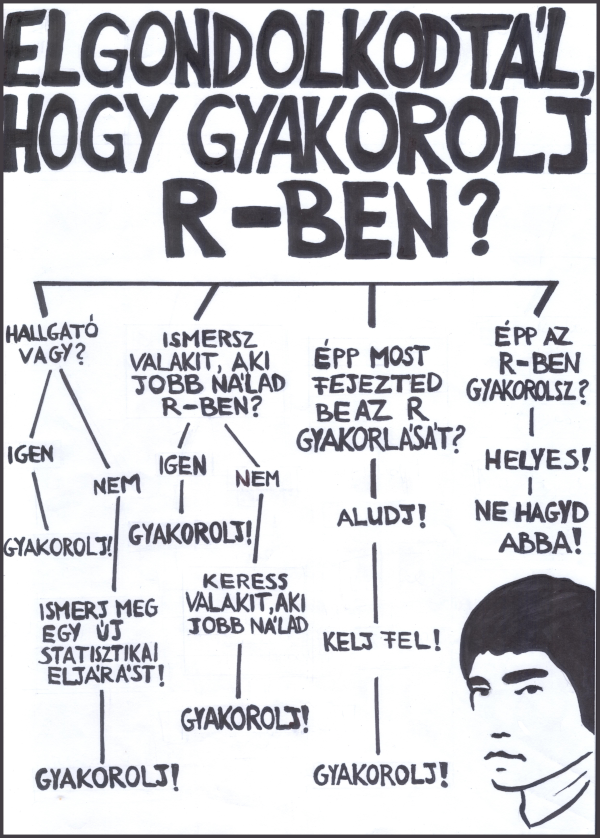
\includegraphics[width=0.7\linewidth]{images/ch_04_small} \end{center}

\hypertarget{AzRStudiohasznalata}{%
\section{Az RStudio használata}\label{AzRStudiohasznalata}}

\begin{rmdlevel1}
Ebben a fejezetben:

\begin{itemize}
\tightlist
\item
  megismerjük az \emph{RStudio} jellemzőit és felépítését,
\item
  a konzolos és parancsállományos használat különbségeit,
\item
  a parancsállományok és az RMarkdown állományok lehetőségeit,
\item
  a projekt fogalmát és használatát,
\item
  és az \emph{RStudio} billentyűparancsait.
\end{itemize}
\end{rmdlevel1}

Miután minden szükséges szoftverkomponenst feltelepítettünk, hogyan tudjuk működésre bírni az R-t?\\
Tegyük fel, hogy van egy nagyon egyszerű adatfeldolgozási problémánk, szeretnénk megtudni a \emph{Csillagok háborúja} c.~film karaktereinek átlagos testmagasságát a filmben szereplő egyes fajokra jellemzően. Ha rátalálunk egy alkalmas adatbázisra, amely tartalmazza a szereplők testmagasságait és azt, hogy melyik fajhoz tartoznak, akkor még két konkrét adatelemzési lépés vár ránk:

\begin{enumerate}
\def\labelenumi{\arabic{enumi}.}
\tightlist
\item
  az adatbázis megnyitása,
\item
  az átlagos testmagasságok meghatározása fajonként.
\end{enumerate}

Korábban láttuk, hogy az R parancssoros, tehát a fenti két lépést R parancsok formájában kell megfogalmaznunk. Azonban több kérdés is felmerül ezen a ponton:

\begin{enumerate}
\def\labelenumi{\arabic{enumi}.}
\tightlist
\item
  hová írjuk a parancsainkat,
\item
  hogyan hajthatjuk őket végre, és végül,
\item
  hol jelenik meg az eredmény.
\end{enumerate}

Ebben a fejezetben a fenti három kérdésekre fókuszálunk, és azt a kérdést, hogy mely konkrét parancsokkal érhetjük el a célunkat a könyv további fejezeteire halasztjuk.

Máris megválaszoljuk a kérdéseket. Korábban láttuk, hogy az \emph{Alap R} telepítésével elérhetővé válik a \emph{konzol}, ahová parancsainkat begépelve, majd \texttt{ENTER}-t ütve utasításokat tudunk végrehajtani. Az \emph{RStudio} telepítésével is kapunk egy konzolt, amelynek működése megegyezik az \emph{Alap R} konzoljával: ide is gépelhetünk parancsokat, és \texttt{ENTER}-rel végrehajthatjuk őket. A parancsok eredmény is itt, a konzolban fog megjelenni.

A kiinduló adatelemzési feladatunk megoldásához tehát vagy az \emph{Alap R} vagy az \emph{RStudio} konzoljába gépeljük be a következő parancsokat, sorról-sorra, és minden egyes sor végén üssünk \texttt{ENTER}-t (a konzol használatához a \ref{az-rstudio-konzol}. és \ref{az-rstudio-konzol}. fejezetekben találunk segítséget). A \texttt{\#}-el kezdődő részeket nem szükséges begépelnünk, azok nem az R-nek szólnak, hanem a megjegyzés szerepét töltik be.

\begin{Shaded}
\begin{Highlighting}[]
\FunctionTok{install.packages}\NormalTok{(}\StringTok{"dplyr"}\NormalTok{)      }\CommentTok{\# a dplyr csomag telepítése}
\FunctionTok{install.packages}\NormalTok{(}\StringTok{"psych"}\NormalTok{)      }\CommentTok{\# a psych csomag telepítése}
\FunctionTok{data}\NormalTok{(starwars, }\AttributeTok{package=}\StringTok{"dplyr"}\NormalTok{)  }\CommentTok{\# adatbázis beolvasása csomagból}
\CommentTok{\# testmagasság átlagok fajonként}
\NormalTok{psych}\SpecialCharTok{::}\FunctionTok{describeBy}\NormalTok{(starwars}\SpecialCharTok{$}\NormalTok{height, starwars}\SpecialCharTok{$}\NormalTok{species, }\AttributeTok{fast=}\NormalTok{T, }\AttributeTok{mat=}\NormalTok{T)}
\end{Highlighting}
\end{Shaded}

A konzol azonban nem a legkényelmesebb módja az R parancsok végrehajtásának. Ezzel minden bizonnyal egyet értenek azok, akik a fenti sorok begépelését és végrehajtását valóban elvégezték a konzolban. A konzolba gépelés helyett érdemes egy szöveges állományban összegyűjteni az adatfeldolgozáshoz kapcsolódó R parancsainkat, ugyanis ezeket később kényelmesen elküldhetjük a konzolba végrehajtásra, pont úgy, mintha közvetlenül a konzolba gépeltük volna be őket. Ezeknek a szöveges állományoknak két fajtáját ismerjük meg ebben a könyvben: a \emph{parancsállományokat} és az \emph{RMarkdown állományokat} (a \ref{publikacio}. fejezetben az RMarkdown állományokról többet olvashatunk).

A parancsállományok és az RMarkdown állományok létrehozásához is a legtöbb segítséget az \emph{RStudio} nyújtja: a parancsok begépelését drámaian leegyszerűsíti, és egyben számos más kényelmi funkciót is ajánl. Hová írjuk tehát az R parancsainkat? A legjobb válasz erre a kérdésre: az \emph{RStudio} parancsállományaiba vagy RMarkdown állományaiba. Mielőtt valóban elvégeznénk ezen állományok létrehozását, ismerkedjünk meg az \emph{RStudio} lehetőségeivel!

\hypertarget{az-rstudio-jellemzux151i}{%
\subsection{Az RStudio jellemzői}\label{az-rstudio-jellemzux151i}}

Fontos tisztázni, az \emph{RStudio} használatához feltétlenül szükség van a telepített \emph{Alap R}-re, nélküle nem tudunk R parancsokat futtatni. Jó gyakorlat, ha az \emph{RStudio} telepítése előtt telepítjük fel az \emph{Alap R}-t, de a fordított sorrend sem okoz problémát. Sőt, ha az \emph{Alap R} egy új verzióját telepítjük fel, akkor a korábban telepített \emph{RStudio} már az új verziójú R futtató környezetét fogja használni. Az \emph{RStudio} tudása tehát a végrehajtható R parancsok tekintetében megegyezik az \emph{Alap R} tudásával, hiszen minden utasítás, amelynek a végrehajtását az \emph{RStudio}-ban kezdeményezzük, végső soron az \emph{Alap R}-rel telepített interpreterhez kerül, és a végrehajtásáért ő felel (\ref{fig:alaprst03}. ábra).

\begin{figure}

{\centering \href{}{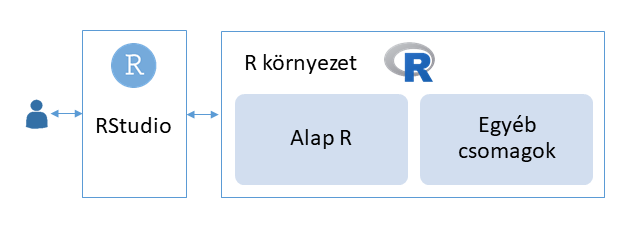
\includegraphics[width=0.85\linewidth]{images/alaprst02} }

}

\caption{Az R kényelmes használata}\label{fig:alaprst03}
\end{figure}

Az \emph{RStudio} elsősorban a parancsok írását könnyíti meg, segítségével a parancsok létrehozásához kapunk rendkívüli segítséget. Megjegyezzük, hogy az \emph{RStudio} egy üzleti vállalkozás neve is egyben, amely többféle terméket fejleszt. Ezek egyike az \emph{RStudio}-nak nevezett integrált fejlesztőkörnyezet, kimondottan az R programozási nyelv számára. Foglaljuk össze, hogy melyek az \emph{RStudio} erősségei:

\begin{itemize}
\tightlist
\item
  \textbf{Parancsok írásának könnyítése.} Az R parancsok begépelését számos eszköz segíti, például a kódkiegészítés, a szintaxisnak megfelelő kódszínezés és a tippek megjelenítése.
\item
  \textbf{Integrált környezetben, egy felületen látjuk a munka során szükséges összes komponenst.} Az adatelemzési munka nem merül ki a parancsok begépelésében és végrehajtásában. Az R parancsokat jelentő forráskódon kívül kezelnünk kell az outputot, ami lehet szöveges és ábra jellegű is, valamint el kell igazodnunk a memóriában tárolt adatok között is. Sokszor a súgót is meg kell jelenítenünk, és információval kell rendelkeznünk a telepített csomagokról is. Az \emph{RStudio} nagy előnye, hogy mindezt egyetlen integrált felületen láthatjuk és ezen keresztül vezérelhetjük.
\item
  \textbf{Projektek használata.} Az \emph{RStudio} támogatja a projektek használatát is, amellyel az adott adatfeldolgozási folyamat összetevőit -- az adatállományokat, parancsállományokat, RMarkdown állományokat, képállományokat és dokumentációkat --, egyetlen könyvtárba foghatjuk össze, és a forráskódból relatívan hivatkozhatunk ezekre az állományokra.
\item
  \textbf{Publikálás támogatása.} Az RMarkdown segítségével kényelmesen és reprodukálható módon hozhatunk létre például PDF, HTML és Word formanyelvű dokumentumokat, vagy PDF, HTML és PowerPoint bemutatókat.
\item
  \textbf{További lehetőségek.} Az \emph{RStudio} támogatja a Shiny Webes alkalmazások fejlesztését, de saját csomagok létrehozásához is kapunk segítséget. Az \emph{RStudio} támogatja a Git verziókezelő használatát is.
\end{itemize}

Az \emph{RStudio} fenti lehetőségeinek bemutatása külön könyvet igényelne, de a mindennapi munkához szükséges ismereteket most bemutatjuk.

\hypertarget{az-rstudio-felepitese}{%
\subsection{Az RStudio felépítése}\label{az-rstudio-felepitese}}

Az \emph{RStudio} indítása után egy több panelból álló alkalmazást látunk. Első indításnál három részre van osztva az alkalmazás, vagyis három panel látható, de a tipikus használat során négy panelünk van. Válasszuk ki először a \texttt{File\ /\ New\ file\ /\ New\ R\ Script} menüpontot, amely egy új parancsállomány létrehozását kezdeményezi. E lépés után már biztosan a négy-paneles, \ref{fig:rstudio-01}. ábrán látható elrendezést kapjuk. Az ábrán megneveztük az egyes részeket, a két bal oldali panel a \emph{Forrás} és a \emph{Konzol}, a jobb oldaliak a \emph{Környezet} és az \emph{Ábra}. Figyeljük meg, hogy a panelek tetején fülek láthatók, így az egyes paneleken különböző lapokat tudunk kiválasztani, egy panel tehát több lapot is tartalmazhat. A panelek szélessége és magassága állítható, egyrészt az elválasztó sávokat az egér segítségével mozgathatjuk, másrészt a panelek méretező gombjain (az egyes panelek jobb felső sarkában) is kattinthatunk. A méretezés során eltűnhetnek panelek, de a sávok mozgatásával vagy a \texttt{View\ /\ Panes\ /\ Show\ All\ Panes} menüponttal láthatóvá tehetjük az összes panelt.

\begin{figure}

{\centering \href{}{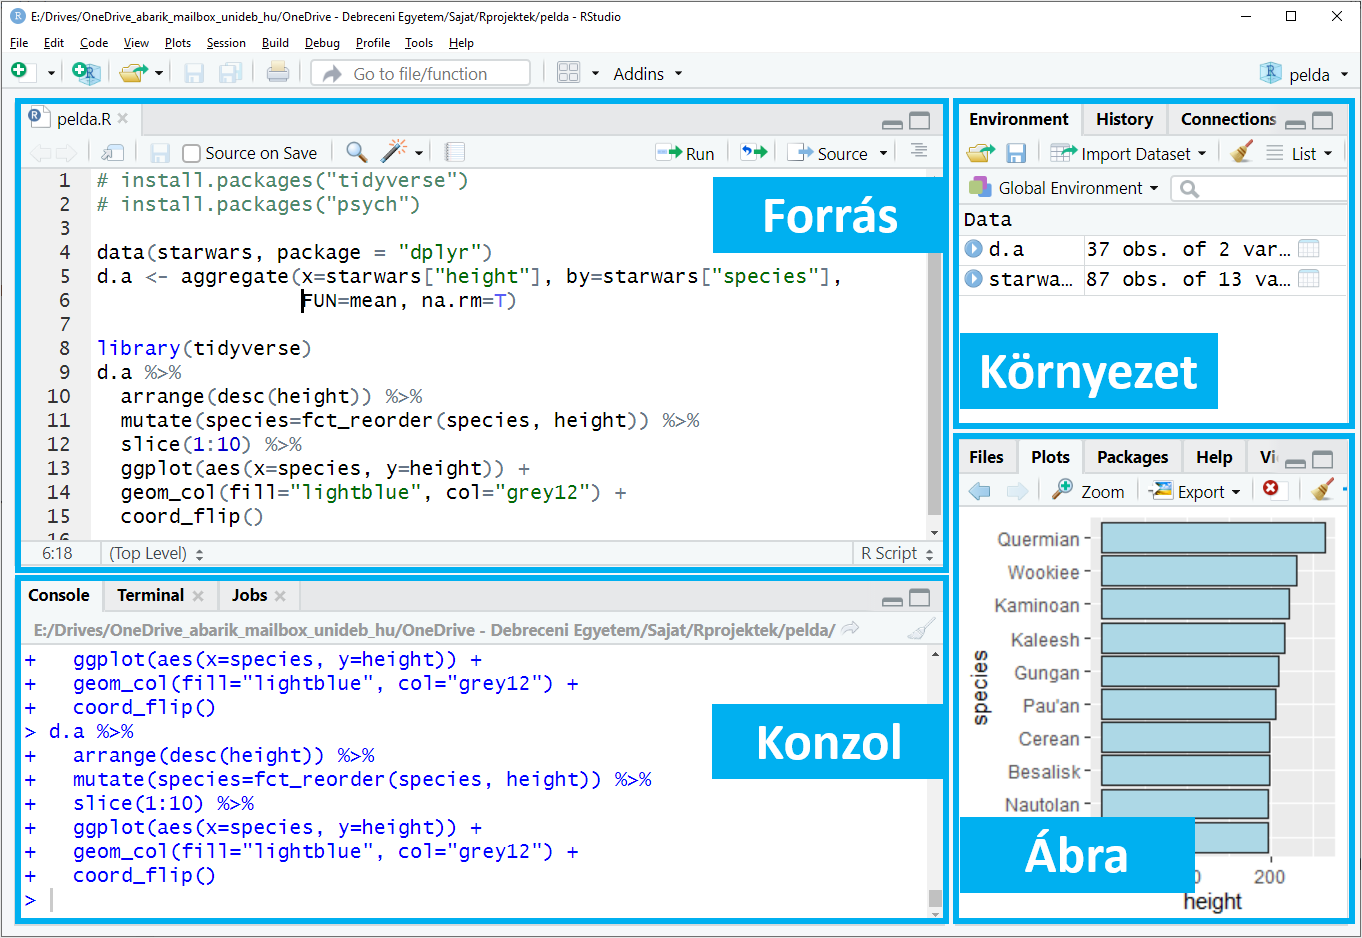
\includegraphics[width=0.85\linewidth]{images/rstudio_01} }

}

\caption{Az RStudio tipikus képernyőképe}\label{fig:rstudio-01}
\end{figure}

A legtöbb időt a \emph{Forrás} nevű bal felső panelben töltjük, mert alapértelmezetten itt jelennek meg a parancsállományok és az RMarkdown állományok lapjai. Az R parancsainkat tehát ide írjuk. Az \emph{RStudio} első indításánál ez a panel üres, de a további indításoknál a korábban szerkesztett, de be nem zárt lapok automatikusan megnyílnak. Itt helyeztünk el korábban egy parancsállomány lapot a \texttt{File\ /\ New\ file\ /\ New\ R\ Script} segítségével. Ez a lap egy egyszerű szövegszerkesztő. Győződjünk meg erről, próbáljuk ki, mert a jövőben ebben a szövegszerkesztőben töltjük a legtöbb időt! A fejezet végi kitűzött feladatok között rákérdezünk a szövegszerkesztési ismeretekre. Oldjuk meg most azt a feladatot, majd térjünk vissza ide!

A bal alsó panel a \emph{Konzol} nevet viseli, vagyis ez az \emph{RStudio} konzolja, melynek használata és célja megegyezik az \emph{Alap R} konzoljával. Vagyis begépelhetünk parancsokat, és az \texttt{ENTER}-rel végrehajtjuk őket. Azonban a konzol mindössze egysoros szövegszerkesztési lehetőséget kínál, lényegében egyszerre egy parancs begépelésére és végrehajtására van lehetőségünk. Ez lényegesen eltér a \emph{Forrás} panel parancsállomány vagy RMarkdown lapján lévő teljes értékű szövegszerkesztőtől, ahol több sor begépelésére és végrehajtására van lehetőségünk. A konzol azonban mégis központi szerepet kap, mert alapesetben az R csak a konzolba kerülő parancsokat tudja végrehajtani. A parancsállományok és RMarkdown állományok R parancsait is valahogyan át kell ide irányítani, úgy mintha ide gépeltük volna be őket. De a konzol nem csak a parancsainkat, azaz az inputot, hanem azok eredményét, az outputot is tartalmazza.

A két jobb oldali panel többfunkciós. A jobb felső, \emph{Környezet} panelben jelennek meg a munka során létrehozott objektumok nevei (\emph{Environment} lap), valamint a parancsok története (\emph{History} lap). Az \emph{Environment} lapon megjelenő adatbázis nevén kattintva a \emph{Forrás} panelben egy külön lapon megjelenik az adatbázis tartalma, így kapjuk az ún. adatbázis lapot. A jobb alsó \emph{Ábra} panel tartalmazza a súgót (\emph{Help} lap), a munka során rajzolt ábráinkat (\emph{Plot} lap), a csomagjaink listáját (\emph{Packages} lap) és a munkakönyvtárunk állományait, könyvtárait (\emph{Files} lap). A két jobb oldali panel elnevezés önkényes volt, hiszen az \emph{Environment} és a \emph{Plot} csak egy-egy lap neve ezeken a többfunkciós paneleken.

\hypertarget{az-rstudio-beuxe1lluxedtuxe1sai}{%
\subsection{Az RStudio beállításai}\label{az-rstudio-beuxe1lluxedtuxe1sai}}

Mielőtt elkezdjük a munkát az \emph{RStudio}-ban feltétlenül módosítsunk néhány alapbeállítást. Az \emph{RStudio} működését az \texttt{Tools\ /\ Global\ Options} menüpont alatt változtathatjuk meg.

\textbf{UTF-8 kódolás beállítása.} A fenti menüpont kiválasztása után a bal oldali listából a \texttt{Code}, majd a fenti opciók közül a \texttt{Saving} opciót válasszuk. A \ref{fig:rstudio-utf8}. ábrán is látható módon, érjük el, hogy a \texttt{Default\ text\ encoding} alatt az \texttt{UTF-8} legyen kiválasztva. Fontos, hogy minden szöveges állományunk UTF-8 kódolású legyen.

\begin{figure}

{\centering \href{}{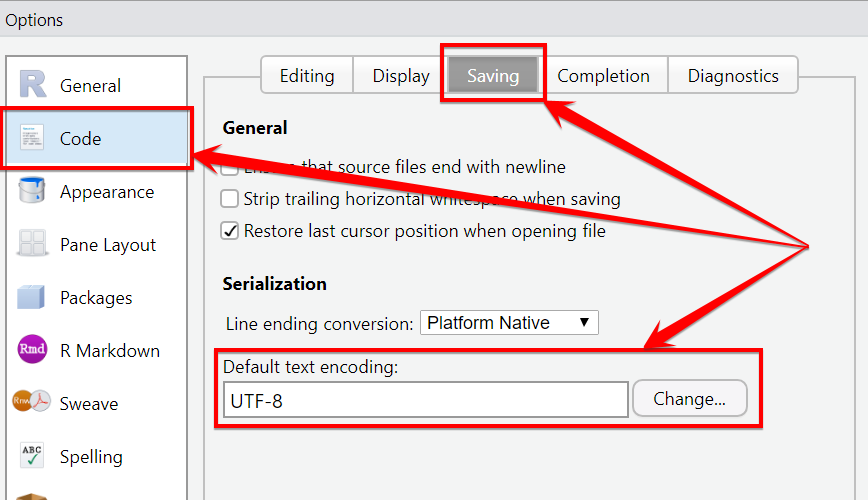
\includegraphics[width=0.7\linewidth]{images/rstudio_utf8} }

}

\caption{Az UTF-8 beállítása az RStudio-ban}\label{fig:rstudio-utf8}
\end{figure}

\textbf{A munkaterület automatikus mentésének tiltása.} A bal oldalon a \texttt{General} menüpont kiválasztása után a \texttt{Basic} opció alatt vegyük ki a pipát a \texttt{Restore\ .RData\ into\ workspace\ at\ startup} elől, valamint a \texttt{Save\ workspace\ to\ .RData\ on\ exit} választót állítsuk \texttt{Never}-re (\ref{fig:rstudio-rdata}. ábra). Az \emph{RStudio} projekt szemléletű használata mellett erre a mentési funkcióra nincs szükség.

\begin{figure}

{\centering \href{}{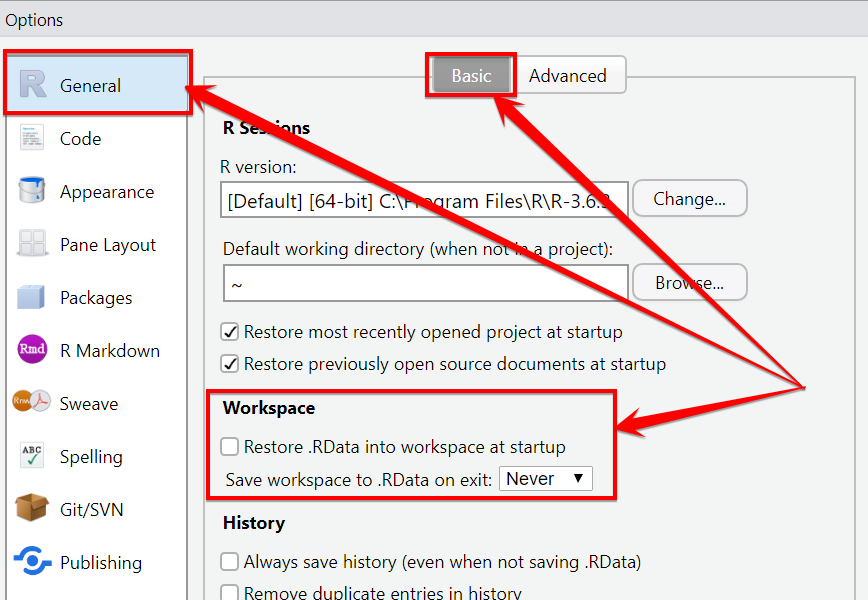
\includegraphics[width=0.7\linewidth]{images/rstudio_rdata} }

}

\caption{A munkaterület automatikus mentésének tiltása az RStudio-ban}\label{fig:rstudio-rdata}
\end{figure}

\textbf{Az output megjelenítésének tiltása az RMarkdown lapon.} A bal oldalon az \texttt{RMarkdown} menüpont kiválasztása után vegyük ki a pipát a \texttt{Show\ output\ inline\ for\ all\ R\ Markdown\ documents} elől (\ref{fig:rstudio-inline}. ábra). Ez a beállítás gördülékenyebb szerkesztést biztosít az RMarkdown lapokon.

\begin{figure}

{\centering \href{}{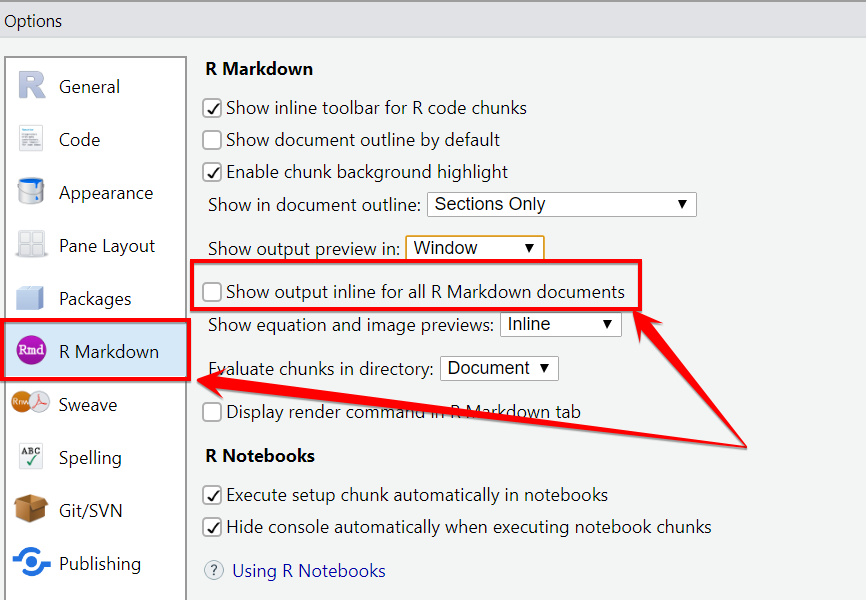
\includegraphics[width=0.7\linewidth]{images/rstudio_inline} }

}

\caption{Az output megjelenítésének tiltása az RMarkdown lapon}\label{fig:rstudio-inline}
\end{figure}

Opcionális lehetőségként a panelek tartalmán is változtathatunk a \texttt{Tools\ /\ Global\ Options\ /\ Pane\ Layout} menüpontban. Az \emph{RStudio} színösszeállításán az \texttt{Appearance} menüpont \texttt{Editor\ theme} beállításával változtathatunk. Javasolt a \texttt{Tomorrow\ Night\ Bright} vagy más, sötétebb háttérszínnel rendelkező téma használata.

\hypertarget{az-rstudio-konzol}{%
\subsection{Az RStudio konzol}\label{az-rstudio-konzol}}

Az \emph{RStudio} konzolja a \emph{Konzol} panel egyik lapján található (\ref{fig:rstudio-01}. ábra). A konzol az \emph{RStudio} kulcsfontosságú része, korábban láttuk, hogy minden R parancsot a végrehajtás előtt ide kell irányítani. Végrehajtása után a szöveges eredmények is itt jelennek meg, és a hibaüzeneteket is itt olvashatjuk. Láthatjuk tehát, hogy a konzol figyelmünk középpontjában áll a munka során.

Közvetlenül azonban nagyon ritkán gépelünk parancsot a konzolba, erre a \emph{Forrás} panel parancsállomány vagy RMarkdown lapját fogjuk használni. Ebben a részben mégis a konzolt mutatjuk be, ugyanis meghatározó szerepe miatt értenünk kell működését.

A konzol működése nagyon egyszerű:

\begin{enumerate}
\def\labelenumi{\arabic{enumi}.}
\tightlist
\item
  egysoros parancsokat gépelünk be a \texttt{\textgreater{}} prompt után,
\item
  \texttt{ENTER}-t nyomunk,
\item
  az R interpreter értelmezi és végrehajtja a begépelt parancsot, és
\item
  megjelenik az eredmény vagy egy hibaüzenet.
\end{enumerate}

Ezt követően egy újabb sor begépelésére van lehetőségünk, \texttt{ENTER} után annak az értelmezése következhet, majd az eredmény megjelenítése jön, és így tovább.

Próbáljuk ki mi is a konzolt! Bátran gépeljünk be parancsokat. Például a \texttt{citation()} parancs outputja fontos lehet az R-el végzett munkáink publikálásánál, hiszen megmutatja hogyan hivatkozhatunk az R statisztikai programra, vagy valamelyik csomagjára.

\begin{Shaded}
\begin{Highlighting}[]
\AttributeTok{\textgreater{} citation()}
\AttributeTok{\textgreater{} citation(package = "ggplot2")}
\end{Highlighting}
\end{Shaded}

Fontos információ az \emph{Alap R} és az \emph{RStudio} pontos verziószáma, ezt a információt az \texttt{R.Version()} és a \texttt{RStudio.Version()} függvény szolgáltatja. Gépelésnél vigyázzunk a kis- és nagybetűk helyes bevitelére, mert az R megkülönbözteti ezeket.

\begin{Shaded}
\begin{Highlighting}[]
\AttributeTok{\textgreater{} R.Version()       }
\AttributeTok{\textgreater{} RStudio.Version()}
\end{Highlighting}
\end{Shaded}

A konzol lehetőségeinek szisztematikus megismerését folytassuk egy egyszerű paranccsal:

\begin{Shaded}
\begin{Highlighting}[]
\AttributeTok{\textgreater{} 1+2}
\CommentTok{[}\OtherTok{1}\CommentTok{]}\AttributeTok{ 3}
\end{Highlighting}
\end{Shaded}

A konzolban most is megjelent az eredmény, ahogy ezt az összes eddigi parancsunk esetében láthattuk. Azonban nem minden parancs után jelenik meg output a konzolban. Például a következő parancsnak nincs eredménysora a konzolban, de ez messze nem jelenti azt, hogy nem történt semmi (történt: létrehoztunk egy objektumot).

\begin{Shaded}
\begin{Highlighting}[]
\AttributeTok{\textgreater{} x \textless{}{-} 3}
\end{Highlighting}
\end{Shaded}

Sőt, az is előfordulhat, hogy az R nem talált valamit rendben a parancsban. Ekkor természetesen nem hajtja/hajthatja végre a begépelt sort, helyette hibát jelez.

\begin{Shaded}
\begin{Highlighting}[]
\AttributeTok{\textgreater{} Ez nem lesz jó.}
\end{Highlighting}
\end{Shaded}

A válasz a fenti ``parancsra'' az \texttt{Error:\ unexpected\ symbol\ in\ "Ez\ nem"} hibaüzenet lesz. Alapvető szabály, ha a válaszban megjelenik az \texttt{Error} szócska, akkor a parancsunkat valamilyen ok miatt nem tudta végrehajtani az R értelmező, és az \texttt{Error} utáni részből tájékozódhatunk a hiba okáról. Minden más esetben sikeres volt a végrehajtás.

Hosszabb, bonyolult parancsok gépelésénél gyakran előfordul, hogy valamiért nem sikerül ``teljessé'' tenni a begépelt parancsot, valami még hiányzik belőle (például egy záró kerek zárójel). Ezt az R értelmező észreveszi és az \texttt{ENTER} megnyomása után egy \texttt{+} folytatás prompt megjelenítésével jelzi ezt számunkra. A \texttt{+} prompt után van lehetőségünk a hiányzó részek pótlására, majd ha készen vagyunk az \texttt{ENTER} billentyűvel az összes eddig még végre nem hajtott sort elküldhetjük az értelmezőnek.

Gépeljük be a következő parancsot, három egymás utáni sorba, \texttt{ENTER}-ekkel elválasztva.

\begin{Shaded}
\begin{Highlighting}[]
\AttributeTok{\textgreater{} paste("Ez már",}
\SpecialStringTok{+        }\NormalTok{"jó"}
\SpecialStringTok{+       }\NormalTok{)}
\CommentTok{[}\OtherTok{1}\CommentTok{]}\NormalTok{ "Ez már jó"}
\end{Highlighting}
\end{Shaded}

A \texttt{paste("Ez\ már",} kerüljön az első sorba, majd nyomjunk \texttt{ENTER}-t. Az R nem hajtja végre a sort, de erre a nyilvánvalóan hibás, befejezetlen parancsra hibaüzenetet sem jelenít meg. Helyette felajánlja a parancs folytatását, befejezését egy új sorban, amely már a \texttt{+} prompttal kezdődik. A második sorba gépeljük be az \texttt{"jó"} karaktersorozatot, nyomjuk meg az \texttt{ENTER}-t. Sajnos még ez sem tette teljessé a parancsunkat, így további folytatásra van lehetőségünk a \texttt{+} után a harmadik sorban. Ide gépeljük be a hiányzó \texttt{)} részt, és üssünk \texttt{ENTER}-t. A parancsunk teljessé vált, megkapjuk az eredményt a konzolban, pontosan úgy, mintha a három sort egyetlen sorba gépeltük volna.

Legyünk nagyon óvatosak a konzol folytatás prompt funkciójával. Ha például az R nem találja a parancs hiányzó részét, akkor a konzol ezen kényelmi funkciója oda vezethet, hogy folyamatosan a \texttt{+} promptot kapjuk az \texttt{ENTER} megnyomása után. Ezt a helyzetet hivatott megoldani az \texttt{ESC} billentyű, mellyel megszakíthatjuk az értelmező parancsfeldolgozási kísérletét. Az \texttt{ESC} megnyomása után visszakapjuk a \texttt{\textgreater{}} prompttal kezdődő (üres) sort, vagyis tiszta lappal, új, lehetőség szerint teljes parancs gépelésébe kezdhetünk. \textbf{A parancssorba mindig teljes parancsot gépeljünk, amint megjelenik a \texttt{+} folytatás prompt, azonnal szakítsuk meg az \texttt{ESC} megnyomásával az értelmezési folyamatot.}

Az R konzolos használatát két funkció valóban kényelmesebbé teszi. Egyrészt a korábban végrehajtott parancsainkat visszahívhatjuk, lapozhatunk bennük előre, hátra. Erre a \texttt{FEL/LE\ NYÍL} billentyűkkel van lehetőségünk. Ezt \emph{history}-nak is nevezzük, vagyis a parancsok történetének. Természetesen, az így visszahívott parancsot tetszőleges módon átszerkeszthetjük: navigálhatunk a sorban előre hátra, beszúrhatunk/törölhetünk karaktereket vagy használhatjuk a vágóasztal billentyűparancsait. A visszahívott és módosított parancsot az \texttt{ENTER} segítségével újra végrehajthatjuk, és ehhez még a sor végére sem kell a szövegkurzort pozicionálni, az a sorban tetszőleges helyen állhat, az R mégis a teljes sort fogja értelmezni.

A másik kényelmi lehetőség a \texttt{TAB} billentyű használata, amellyel az elkezdett, de még be nem fejezett sorokat egészíthetjük ki. Ha egy sort többféleképpen is kiegészíthet az R, akkor egy listát kapunk a lehetőségekről, amelyet továbbgépeléssel szűkíthetünk, ha pedig csak egyetlen szóba jöhető befejezése van a begépelt karaktereknek, akkor a \texttt{TAB} megnyomása után ezzel a résszel kiegészül az elkezdett sorunk. Így nemcsak egyszerűen gépelést, illetve időt takaríthatunk meg, hanem például tájékozódhatunk a korábban létrehozott objektumok nevéről vagy az elérhető függvények névéről és paramétereiről is.

Az objektum, a függvények és az egyéb ebben a fejezetben homályosan hagyott fogalmak definícióit a könyv későbbi részeiben részletesen tárgyaljuk.

\hypertarget{parancsallomanyok}{%
\subsection{Parancsállományok}\label{parancsallomanyok}}

Láthattuk, hogy a konzolba egyszerre csak egy parancsot gépelhetünk be, úgy is gondolhatunk a konzolra, mint egy egysoros szövegszerkesztőre. Begépelünk egy sort és végrehajtjuk az \texttt{ENTER}-rel. A problémáink többsége viszont nem oldható meg egyetlen paranccsal, csak több tízzel vagy százzal, ezért ez az interaktív, \emph{konzolos használat} nem alkalmas hosszabb elemzésre.

Parancsainkat begépelhetjük egy \texttt{.R} kiterjesztésű, egyszerű, formázás nélküli szöveges állományba is. Az ilyen szöveges állományt \emph{parancsállomány}nak vagy \emph{szkriptállomány}nak nevezzük. Ilyen szöveges állományok létrehozására tetszőleges szövegszerkesztő alkalmas, de természetesen mi az \emph{RStudio} segítségével fogjuk ezeket elkészíteni, ugyanis itt kapjuk a legnagyobb segítséget a parancsok gépeléséhez, majd végrehajtásához. A \emph{Forrás} panel tartalmazza a parancsállomány lapokat, létrehozásuk a korábban látott \texttt{File\ /\ New\ file\ /\ New\ R\ Script} menüponttal történik. Parancsállományok mentésére és már létező megnyitására is van lehetőségünk a megfelelő menüpont kiválasztásával (\texttt{File\ /\ Save} és \texttt{File\ /\ Open\ File}).

A parancsállományok használata lényegesen leegyszerűsíti az adatelemzés folyamatát, hiszen a konzol egysoros szövegszerkesztője helyett egy szinte végtelen sok parancssor begépelésére alkalmas szövegszerkesztő áll rendelkezésünkre. Mint minden szövegszerkesztőben, a különböző billentyűparancsok és a vágóasztal itt is megkönnyíti szerkesztés folyamatát. Az \texttt{ENTER} jelentése parancsállományos környezetben a szövegszerkesztőkben megszokott újsor beszúrása, ami lényegesen különbözik a konzolos használat parancs végrehajtási funkciójától. A parancsaink interaktív végrehajtásáért az \emph{RStudio}-ban a \texttt{Code/Run\ selected\ line(s)} menüpont, vagy még gyakrabban a \texttt{Ctrl+Enter} billentyűkombináció felel. Ezekkel a módszerekkel tudjuk a parancsainkat a konzolba irányítani és végrehajtani. De nézzük meg ezt a gyakorlatban!

\hypertarget{munka-az-rstudio-ban}{%
\subsection{Munka az RStudio-ban}\label{munka-az-rstudio-ban}}

Kezdjük a munkát! Nyissunk egy új parancsállományt (\texttt{File\ /\ New\ file\ /\ New\ R\ Script}) és gépeljünk be néhány sort. Figyeljük meg, hogy milyen sokat segít az \emph{RStudio} a lenti sorok begépelésében. Az értékadás (\texttt{\textless{}-}) operátort az \texttt{Alt+-} billentyűkombináció segítségével vigyük be.

\begin{Shaded}
\begin{Highlighting}[]
\DecValTok{1}\SpecialCharTok{+}\DecValTok{23}
\FunctionTok{getwd}\NormalTok{()          }\CommentTok{\# munkakönyvtár kiírása}
\NormalTok{x }\OtherTok{\textless{}{-}} \FunctionTok{mean}\NormalTok{(}\DecValTok{1}\SpecialCharTok{:}\DecValTok{100}\NormalTok{)}
\FunctionTok{plot}\NormalTok{(}\DecValTok{1}\SpecialCharTok{:}\DecValTok{10}\NormalTok{)}
\NormalTok{?mean}
\FunctionTok{cat}\NormalTok{(}\StringTok{"{-} Vége {-}}\SpecialCharTok{\textbackslash{}n}\StringTok{"}\NormalTok{)}
\end{Highlighting}
\end{Shaded}

A szövegkurzorral álljunk az első sorra, és hajtsuk végre \texttt{Ctrl+Enter} billentyűparancsot. Láthatjuk, hogy (1) a sor átkerül a konzolba, (2) az \emph{RStudio} végrehajtja a sort és az eredményt a konzolban megjeleníti, és (3) a szövegkurzor lejjebb lép a következő végrehajtható sorra. Egy újabb \texttt{Ctrl+Enter} így már ezt a sort hatja végre, és így tovább. Ha a sorok végrehajtása közben hibaüzenetet kapunk (\texttt{Error}), ne essünk kétségbe, a hibaüzenet a munka része. Nézzük át figyelmesen a begépelt sorainkat, javítsuk őket, és futtassuk újra az összes sort, fentről lefelé a \texttt{Ctrl+Enter}-ek segítségével.

A parancsok végrehajtása során láthatjuk mennyire kényelmes, integrált környezetben találtuk magunkat. Az \texttt{x\ \textless{}-\ mean(1:100)} hatására az \emph{Environment} lapon megjelent az \texttt{x} objektum neve és értéke. A \emph{Plot} lapon láthatunk egy ábrát, amit a \texttt{plot(1:10)} rajzolt meg, és a \texttt{?mean} a \emph{Help} lapon mutatja meg a \texttt{mean()} átlagszámoló függvény beépített súgóját.

Mentsük el parancsállományunkat a \texttt{File\ /\ Save} vagy a \texttt{Ctrl+S} segítségével. Korábban létrehozott parancsállományokat a \texttt{File\ /\ Open} menüponttal nyithatunk meg.

A soronkénti végrehajtás mellett nagyon gyakori a kijelölt szövegrészek végrehajtása, amit szintén a \texttt{Ctrl+Enter}-rel tudunk kezdeményezni. A kijelölt rész lehet több sor, a teljes parancsállomány, vagy valamelyik sor egy része. Ez utóbbi próbáljuk ki úgy, hogy a parancsállomány első sorában csak az \texttt{1+2} részt jelöljük ki, és ezt hajtsuk végre a \texttt{Ctrl+Enter} segítségével. Az eredmény a konzolban a 3 lesz. A teljes szkriptállomány végrehajtásához jelöljük ki \texttt{Ctrl+A} segítségével a parancsállomány összes sorát, és nyomjuk meg a \texttt{Ctrl+Enter}-t. A konzolban tudjuk ellenőrizni, hogy minden sort újra végrehajtottunk.

Térjünk vissza a kiinduló adatelemzési problémánk megoldásához. Láttuk, hogy az R parancsok összegyűjtésére és végrehajtására a \texttt{.R} kiterjesztésű parancsállományok kiváló megoldást nyújtanak. Emlékezzünk vissza a fejezet eleji példára, amelyben a Csillagok háborúja c.~film karaktereinek átlagos testmagasságát kerestük. Nyissunk egy új parancsállományt (\texttt{File\ /\ New\ file\ /\ New\ R\ Script}) és gépeljük be a megoldást jelentő sorokat.

\begin{Shaded}
\begin{Highlighting}[]
\CommentTok{\# A Csillagok háborúja c. film karaktereinek átlagos testmagassága}
\CommentTok{\# Abari Kálmán}
\CommentTok{\# 2022. 07. 06.}

\CommentTok{\# install.packages("dplyr")      \# a dplyr csomag telepítése}
\CommentTok{\# install.packages("psych")      \# a psych csomag telepítése}
\FunctionTok{data}\NormalTok{(starwars, }\AttributeTok{package=}\StringTok{"dplyr"}\NormalTok{)  }\CommentTok{\# adatbázis beolvasása csomagból}
\CommentTok{\# testmagasság átlagok fajonként}
\NormalTok{psych}\SpecialCharTok{::}\FunctionTok{describeBy}\NormalTok{(starwars}\SpecialCharTok{$}\NormalTok{height, starwars}\SpecialCharTok{$}\NormalTok{species, }\AttributeTok{fast=}\NormalTok{T, }\AttributeTok{mat=}\NormalTok{T)}
\end{Highlighting}
\end{Shaded}

Látható, hogy a feladat tényleges megoldását jelentő két R parancs mellett megjegyzéseket is becsempésztünk, hogy később is tudjuk, ki, mikor és miért készítette ezt a parancsállományt (a \texttt{\#} utáni részeket a sor végéig az R figyelmen kívül hagyja; részletesebb információkat a megjegyzésekről a \ref{MegjegyzesazRben}. fejezetben olvashatunk). Futtassuk a sorokat a \texttt{Ctrl+Enter} segítségével, fussuk át a kiszámolt átlagos testmagasságokat az output \texttt{mean} oszlopában, majd mentsük el a szkriptállományt \texttt{Ctrl+S}-sel \texttt{starwars.R} néven. Később, napok, hetek vagy hónapok múlva, újra megnyithatjuk \texttt{starwars.R} állományunkat (\texttt{File\ /\ Open}), és újra lefuttathatjuk mini-elemzésünket. Ezzel a fejezet eleji adatelemzési feladatunkat megoldottuk. Vajon lehet ezt ennél jobban csinálni? Igen!

\hypertarget{rmarkdown-allomanyok}{%
\subsection{RMarkdown állományok}\label{rmarkdown-allomanyok}}

Az R parancsainkat olyan \texttt{.Rmd} kiterjesztésű, egyszerű, szöveges állományokban is összegyűjthetjük, amelyek többet nyújtanak, mint a parancsállományok, de szerkezetük kicsit kötöttebb. Az ilyen szöveges állományok az RMarkdown állományok. Miben nyújtanak többet: ahogyan a \ref{publikacio}. fejezetben részletesen áttekintjük, az RMarkdown állományok az eredmények publikálásához, például HTML, PDF vagy Word formanyelvű állományok létrehozását teszik lehetővé.

Hozzunk létre az \emph{RStudio}-ban a \texttt{File\ /\ New\ File\ /\ R\ Markdown} menüponttal egy új RMarkdown állományt. A megjelenő dialógusdobozban töltsük ki a \texttt{Title} és \texttt{Author} mezőket, azaz adjunk címet és szerzőt a dokumentumhoz, majd kattintsunk az \texttt{OK} gombon. A \texttt{Forrás} panelen megjelenik egy új RMarkdown lap, amely egy alapértelmezett tartalommal jön létre, és nem üresen, mint a parancsállományok esetében. Említettük, hogy az RMarkdown állományok szerkezete kötöttebb, ez az alapértelmezett tartalom az eligazodásban segít minket. Érjük el, hogy az új RMarkdown ezeket a sorokat tartalmazza (a szerző neve a sajátunk legyen):

\begin{Shaded}
\begin{Highlighting}[]
\CommentTok{{-}{-}{-}}
\AnnotationTok{title:}\CommentTok{ "A Csillagok háborúja c. film karaktereinek átlagos testmagassága"}
\AnnotationTok{author:}\CommentTok{ "Abari Kálmán"}
\AnnotationTok{date:}\CommentTok{ \textquotesingle{}2022. 07. 06.\textquotesingle{}}
\AnnotationTok{output:}\CommentTok{ html\_document}
\CommentTok{{-}{-}{-}}

\InformationTok{\textasciigrave{}\textasciigrave{}\textasciigrave{}\{r setup, include=FALSE\}}
\InformationTok{knitr::opts\_chunk$set(echo = TRUE)}
\InformationTok{\textasciigrave{}\textasciigrave{}\textasciigrave{}}

\NormalTok{Adatok beolvasása és az átlagok kiírása}

\InformationTok{\textasciigrave{}\textasciigrave{}\textasciigrave{}\{r\}}
\InformationTok{\# install.packages("dplyr")      \# a dplyr csomag telepítése}
\InformationTok{\# install.packages("psych")      \# a psych csomag telepítése}
\InformationTok{data(starwars, package="dplyr")  \# adatbázis beolvasása csomagból}
\InformationTok{\# testmagasság átlagok fajonként}
\InformationTok{psych::describeBy(starwars$height, starwars$species, fast=T, mat=T)}
\InformationTok{\textasciigrave{}\textasciigrave{}\textasciigrave{}}
\end{Highlighting}
\end{Shaded}

Minden RMarkdown állomány egy fejléccel kezdődik, amelyet a \texttt{-\/-\/-} karakterek határolnak. A természetes nyelvű szöveget szabadon a fejléc alatti részben bárhová írhatjuk, az R parancsokat azonban ún. R csonkokban kell elhelyeznünk, amelyeket speciális kezdő és záró sorok határolnak. A \ref{publikacio}. fejezetben részletesebben olvashatunk ezekről. Most elégedjünk meg annyival, hogy egy RMarkdown állományban tetszőlegesen sok R csonkot elhelyezhetünk, és egy R csonk tetszőlegesen sok R parancsot tartalmazhat. Egy R csonkon belül a parancsok végrehajtása ugyanúgy \texttt{Ctrl+Enter}-rel történik, mint a parancsállományok esetében. Próbáljuk ki! A most begépelt RMarkdown állományunk második csonkjában lévő két R parancsot hajtsuk végre két \texttt{Ctrl+Enter} segítségével. A mini-elemzés eredménye ismét a konzolban látható.

Hogyan foglalhatnánk össze a parancsállományok és az RMarkdown állományok közötti különbséget? A \ref{tab:parancsrmarkdown}. táblázatban láthatjuk, hogy mindkét állományban összesen három különböző tartalmat szoktunk rögzíteni:

\begin{enumerate}
\def\labelenumi{\arabic{enumi}.}
\tightlist
\item
  fejléc információt arról, hogy mi az elemzés célja, ki és mikor készítette az állományt,
\item
  magyarázó, természetes nyelvű szöveget (pl. magyar vagy angol nyelven), és
\item
  az adatelemző R parancsokat.
\end{enumerate}

Az R parancsokat szabadon írhatjuk a parancsállományokba, viszont a fejléc információt és a magyarázó szövegeket megjegyzésbe kell tenni. Az RMarkdown állományokba a magyarázó, természetes nyelvű szövegek írhatók szabadon, míg az R parancsokat csonkokba, a fejléc információt pedig kötött módon, az állomány elejére kell írnunk.

\begin{longtable}[]{@{}
  >{\raggedright\arraybackslash}p{(\columnwidth - 4\tabcolsep) * \real{0.4020}}
  >{\raggedright\arraybackslash}p{(\columnwidth - 4\tabcolsep) * \real{0.3235}}
  >{\raggedright\arraybackslash}p{(\columnwidth - 4\tabcolsep) * \real{0.2745}}@{}}
\caption{\label{tab:parancsrmarkdown} A parancsállomány és az RMarkdown állomány összehasonlítása}\tabularnewline
\toprule
\begin{minipage}[b]{\linewidth}\raggedright
Tartalom
\end{minipage} & \begin{minipage}[b]{\linewidth}\raggedright
Parancsállomány (\texttt{.R})
\end{minipage} & \begin{minipage}[b]{\linewidth}\raggedright
RMarkdown (\texttt{.Rmd})
\end{minipage} \\
\midrule
\endfirsthead
\toprule
\begin{minipage}[b]{\linewidth}\raggedright
Tartalom
\end{minipage} & \begin{minipage}[b]{\linewidth}\raggedright
Parancsállomány (\texttt{.R})
\end{minipage} & \begin{minipage}[b]{\linewidth}\raggedright
RMarkdown (\texttt{.Rmd})
\end{minipage} \\
\midrule
\endhead
\emph{Fejléc szöveg} & & \\
cím, szerző, dátum & megjegyzésbe & fejlécbe \\
\emph{Magyarázó szöveg} & & \\
természetes nyelvű szöveg & megjegyzésbe & bárhová \\
\emph{Adatelemzés} & & \\
R parancs & bárhová & R csonkba \\
\bottomrule
\end{longtable}

Valóban annyiban áll a különbség a két állománytípus között, hogy a máshová és máshogyan írjuk az R parancsokat és az egyéb magyarázó/fejléc szövegeinket? Nem. A \ref{publikacio}. fejezetben részletesen bemutatjuk, hogy az RMardown állományok ereje abban van, hogy egy fordítási folyamat (\emph{knit}-elés) során, olyan PDF, HTML vagy Word állományt tudunk előállítani, amely a magyarázó/fejléc szövegeken, és az R parancsokon kívül, az R parancsok outputját is tartalmazza, legyen az szöveges vagy ábra jellegű output.

\hypertarget{projektek-hasznalata}{%
\subsection{Projektek használata}\label{projektek-hasznalata}}

Mostanra nagyon közel kerültünk az általunk ajánlott adatelemzési munkaformához, ugyanis már tudunk az \emph{RStudio}-n belül parancsállományokat és RMarkdown állományokat használni. Még egy összetevő azonban kulcsfontosságú a kényelmes munkához: az \emph{RStudio}-ban minden esetben projektet kell használnunk.

Az \emph{RStudio} lehetőséget ad arra, hogy minden egyes adatfeldolgozási feladatunkhoz egy projektet rendeljünk. Egy \emph{RStudio} projekt minimálisan egy projekt könyvtárat és az ebben lévő lévő \texttt{.Rproj} kiterjesztésű projektállományt jelenti. Ezeket a következő módszerrel hozhatjuk létre. Először kattintsunk a \texttt{File\ /\ New\ Project} menüponton. Válasszuk ki a \texttt{New\ Directory} opciót (\ref{fig:rstudio-proj-1}. ábra), majd a \texttt{New\ Project} nyomógombon kattintsunk (\ref{fig:rstudio-proj-2}. ábra).

\begin{figure}

{\centering \href{}{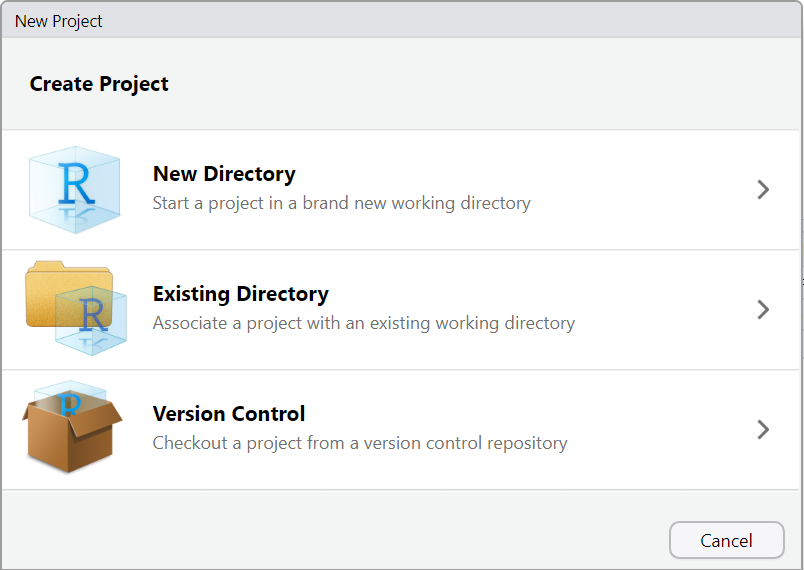
\includegraphics[width=0.65\linewidth]{images/rstudio_proj_1} }

}

\caption{RStudio projekt létrehozása: 1. lépés}\label{fig:rstudio-proj-1}
\end{figure}

A \texttt{Directory\ name} szöveges mezőbe a projektünk nevét határozhatjuk meg, ami egyben az új projektünk könyvtárneve is lesz. Adjuk meg itt az \texttt{elso\_projekt} nevet. A \texttt{Create\ project\ as\ subdirectory\ of} mezőben azt a szülő könyvtárat határozhatjuk meg, ahová a projekt könyvtárunkat el szeretnénk helyezni. Ezt szabadon megválaszthatjuk, lehet az adott felhasználó dokumentumok könyvtára is. A projekt létrehozását a \texttt{Create\ Project} nyomógombbal fejezhetjük be.

\begin{figure}

{\centering \href{}{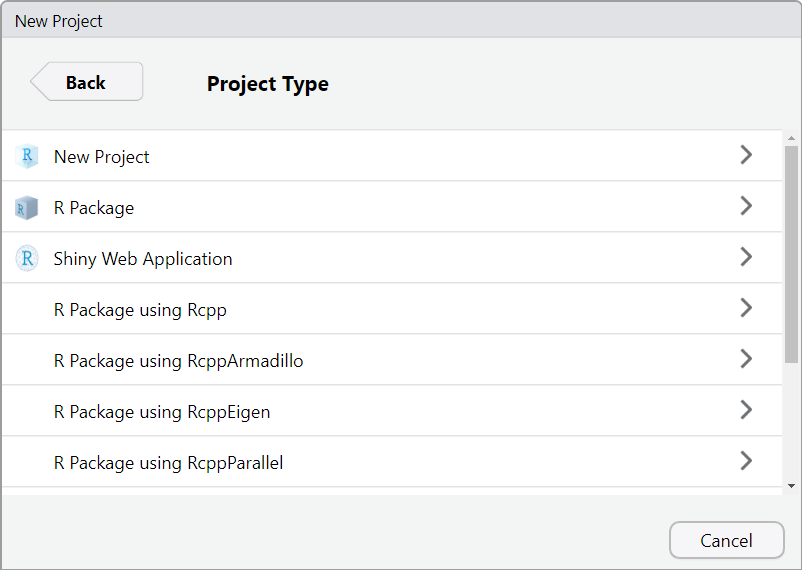
\includegraphics[width=0.65\linewidth]{images/rstudio_proj_2} }

}

\caption{RStudio projekt létrehozása: 2. lépés}\label{fig:rstudio-proj-2}
\end{figure}

Két nagyon fontos dolog történt a fentiek hatására. Egyrészt a számítógépünkön létrejött az \texttt{elso\_projekt} projektkönyvtár, és benne az \texttt{elso\_projekt.Rproj} projektállomány, másrészt az \emph{RStudio} ún. \emph{projekt üzemmód}ba került, azaz az \texttt{elso\_projekt} lesz az aktív projekt. Az \emph{RStudio}-ban egyszerre egy projekt lehet aktív, de elképzelhető, hogy egyetlen projekt sem aktív. Az \emph{RStudio} felületén a jobb felső sarokban tájékozódhatunk, ahol most az \texttt{elso\_project} feliratot látjuk, de amennyiben nincs aktív projektünk, akkor a \texttt{Project:\ (none)} feliratot olvashatjuk. Kerüljük a projekt nélküli állapotot.

\begin{figure}

{\centering \href{}{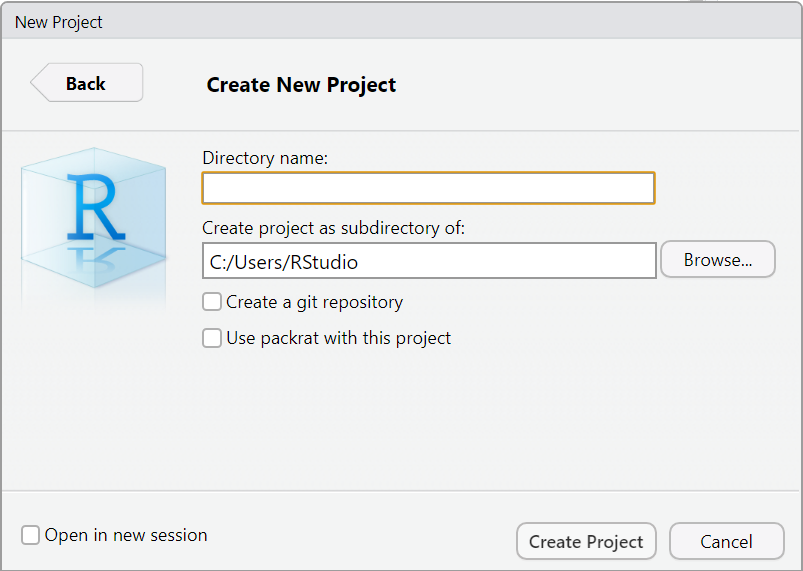
\includegraphics[width=0.65\linewidth]{images/rstudio_proj_3} }

}

\caption{RStudio projekt létrehozása: 3. lépés}\label{fig:rstudio-proj-3}
\end{figure}

Minden adatfeldolgozási feladathoz -- még a legkisebbhez is -- hozzunk létre projektet. Minden állományt, amely a feladathoz tartozik a projektkönyvtáron belül helyezzünk el. Milyen állományok jöhetnek szóba: például parancsállományok, RMarkdown állományok, adatállományok, képállományok, dokumentációk és hivatkozásokat tartalmazó állományok. Érdemes ezeket rendezetten, ha szükséges, alkönyvtárakba szétosztva tárolni. Jó gyakorlat lehet, hogy a parancsállományokat és az RMarkdown állományokat közvetlenül a projektkönyvtárban (most ez az \texttt{elso\_projekt}), az adatállományokat egy \texttt{adat} alkönyvtárban a projektkönyvtáron belül (most \texttt{elso\_projekt/adat}) tároljuk, a képállományok és dokumentációk helye pedig lehet az \texttt{elso\_project/kep}, illetve \texttt{elso\_projekt/doku} alkönyvtár.

Válthatunk egy másik projektre is (\texttt{File\ /\ Open\ Project}), de be is zárhatjuk az aktív projektet (\texttt{File\ /\ Close\ project}). Később újra megnyithatjuk ezt is a \texttt{File\ /\ Open\ Project} segítségével. A megnyitás során természetesen az \texttt{.Rproj} kiterjesztésű projektállományt kell kiválasztanunk.

Ritkábban az is előfordulhat, hogy az adatfeldolgozási folyamatunkkal kapcsolatos állományok összegyűjtését korábban elkezdtük, és csak később szeretnénk ezt a könyvtárat egyben \emph{RStudio} projektkönyvtárként is felhasználni.

\begin{figure}

{\centering \href{}{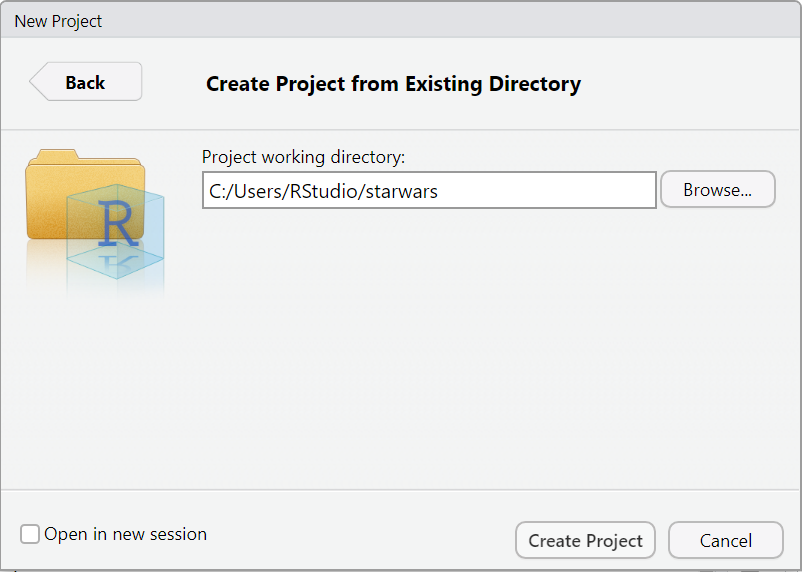
\includegraphics[width=0.65\linewidth]{images/rstudio_proj_4} }

}

\caption{RStudio projekt létrehozása: létező könyvtár megadása}\label{fig:rstudio-proj-4}
\end{figure}

Korábban létrehozott könyvtárból szintén a \texttt{File\ /\ New\ Project} menüpont segítségével hozhatunk létre \emph{RSudio} projektkönyvtárat. Itt azonban az \texttt{Existing\ Directory} opciót kell kiválasztani (\ref{fig:rstudio-proj-1}. ábra). Ezt követően ennek a létező könyvtárnak az elérési útját kell megadnunk az \ref{fig:rstudio-proj-4}. ábrán látható beviteli mezőben.

Végül foglaljuk össze, milyen előnyökkel jár a projekt használata:

\begin{itemize}
\tightlist
\item
  A logikailag egy adatfeldolgozási folyamathoz tartozó állományainkat fizikailag is együtt tudjuk tartani.
\item
  Projekt üzemmódban az \emph{RStudio} az aktuális könyvtárat a projektkönyvtárra állítja, így relatív hivatkozást használhatunk a kódunkban, amely a projekt hordozhatóságát biztosítja különböző számítógépek között.
\end{itemize}

\hypertarget{billenytux171parancsok}{%
\subsection{Billenytűparancsok}\label{billenytux171parancsok}}

Az \emph{RStudio} legfontosabb billentyűparancsa a \texttt{Ctrl+Enter}, amely a parancsot a konzolba küldi végrehajtásra. Van még néhány további billentyűparancs, amelyet érdemes felsorolni, hiszen ezek használatával gyorsítani, egyszerűsíteni tudjuk a munkánkat.

\begin{itemize}
\tightlist
\item
  \texttt{Ctrl+Shift+N}: új parancsállomány létrehozása,
\item
  \texttt{Ctrl+S}: állomány mentése,
\item
  \texttt{Ctrl+W}: lap bezárása a \texttt{Forrás} panelen,
\item
  \texttt{Ctrl+Tab\ /\ Ctrl+Shift+Tab}: aktív lap léptetése előre és hátra a \texttt{Forrás} panelen,
\item
  \texttt{Ctrl+F}: szöveg keresése és cseréje,
\item
  \texttt{Tab}: kód kiegészítése,
\item
  \texttt{Ctrl+Shift+C}: kijelölt sorok be- vagy kikommentelése,
\item
  \texttt{Ctrl+Alt+Fel\ /\ Le} (és \texttt{Shift+Jobbra\ /\ Balra}): a kurzor magasságának állítása (és az oszlopszélesség beállítása) több sor szerkesztésére,
\item
  \texttt{Esc}: a \texttt{Konzol} panelen kilépés a folytatás promptból, a \texttt{Forrás} panelen kilépés a többsoros szerkesztésből,
\item
  \texttt{Alt+Fel\ /\ Le}: sor mozgatása fel vagy le,
\item
  \texttt{Alt+Shift+K}: billentyűparancsok módosítása,
\item
  \texttt{Alt+-}: értékadó operátor (\texttt{\textless{}-}) beszúrása,
\item
  \texttt{Ctrl+Shift+M}: pipe operátor (\texttt{\%\textgreater{}\%}) beszúrása,
\item
  \texttt{Ctrl+Enter}: az aktuális sor vagy a kijelölt rész futtatása,
\item
  \texttt{Ctrl+Alt+R}: a teljes parancsállomány futtatása,
\item
  \texttt{Ctrl+Shift+P}: a kurzor feletti csonkok parancsainak futtatása,
\item
  \texttt{Ctrl++\ /\ Ctrl+-}: betűméret nagyítása vagy kicsinyítése,
\item
  \texttt{Ctrl+Shift+F10}: a munkamenet újraindítása.
\end{itemize}

Ha valamelyik kombináció nem működik a számítógépünkön, akkor a \texttt{Tools\ /\ Modify\ Keyboard\ Shortcuts} menüpont alatt új billentyűparancsot adhatunk az ott felsorolt funkciókhoz.

\hypertarget{munka-az-r-ben-1-summary}{%
\subsection{Összefoglalás}\label{munka-az-r-ben-1-summary}}

\begin{rmdsummary}
Az adatelemzési munka során az \emph{RStudio} -t használjuk projekt
üzemmódban, miközben RMarkdown állományba gyűjtjük az elemző R
parancsokat és az egyéb magyarázó és fejléc szövegeket. Ebben a
fejezetben ezt a tételmondatot töltöttük meg tartalommal. Megismertük az
\emph{RStudio} integrált környezetét. A \emph{Forrás} panel lehetséges
lapjai a parancsállomány, az RMarkdown állomány és az adatbázis. A
\emph{Konzol} panel legfontosabb lapja a \emph{konzol}, amely központi
szerepet játszik a munka során, hiszen a \texttt{Ctrl+Enter}-rel
végrehajtott R parancsok eredménye és az esetleges hibaüzenetek is itt
jelennek meg. A munka során a \texttt{.R} kiterjesztésű
parancsállományok kiválóan alkalmasak a hosszabb elemzések R
parancsainak tárolására, de ha a publikáláshoz is segítséget szeretnénk
kapni, akkor inkább a a kötöttebb szerkezetű \texttt{.Rmd} kiterjesztésű
RMarkdown állományba rögzítsük parancsainkat. Az \emph{RStudio}
rutinszerű használatához a billentyűparancsok ismerete is hozzátartozik.
A projektszemlélet az adatelemzéssel kapcsolatos állományok egyben
tartásáról, és a hordozhatóság biztosításáról szól.
\end{rmdsummary}

\hypertarget{munka-az-r-ben-1-exercise}{%
\subsection{Feladatok}\label{munka-az-r-ben-1-exercise}}

\begin{rmdexercise}
\begin{enumerate}
\def\labelenumi{\arabic{enumi}.}
\tightlist
\item
  Bizonyosudjunk meg róla, hogy az alapvető szövegszerkesztési ismeretek birtokában vagyunk. Ismerjük az \texttt{Insert} billentyű funkcióját? Találjunk legalább 8 módszert, amely kizárólag a billentyű segítségével mozgatja a szövegkurzort! A szövegkijelölésnek milyen billentyűparancsait ismerjük? Milyen karaktertörlési lehetőségeket ismerünk? Ismerjük mindhárom vágóasztal-művelet billentyűparancsát?
\item
  Az \emph{RStudio} mellett milyen más intergrált fejlesztőeszközök léteznek az R-hez?
\item
  Az \texttt{Appearance} menüpont \texttt{Editor\ theme} beállításával változtassunk az \emph{RStudio} színösszeállításán. Keressük meg a legjobban hozzánk illőt! Vegyük figyelembe, hogy hosszútávon a minél sötétebb háttér a jó választás.
\end{enumerate}
\end{rmdexercise}

\hypertarget{seguxedtsuxe9g-az-r-hasznuxe1latuxe1hoz}{%
\section{Segítség az R használatához}\label{seguxedtsuxe9g-az-r-hasznuxe1latuxe1hoz}}

\begin{rmdlevel2}
Ebben a fejezetben:

\begin{itemize}
\tightlist
\item
  megismerjük az R hivatalos dokumentációit,
\item
  az ún. cheet-sheet-ek forrását,
\item
  és a parancssorból elérhető súgó parancsokat.
\end{itemize}
\end{rmdlevel2}

Az R használatához számos segítséget találunk az Interneten, a telepített \emph{Alap R}-ben és az \emph{RStudio}-ban egyaránt. Az online segítségek közül elsősorban a \texttt{http://cran.r-project.org} címen olvasható R dokumentációkat emeljük ki, ahol több tucat, elsősorban angol nyelvű leírást találunk az R megismeréséhez. A bal oldali \texttt{Documentation\ /\ Manuals} menüpont alatt találjuk például az R hivatalos bevezető dokumentumát (\href{https://cran.r-project.org/doc/manuals/r-release/R-intro.html}{\emph{An Introduction to R}}), melynek tanulmányozása rendkívül nagy lépést jelenthet az R alaptudás megszerzéséhez. Az említett menüpont alatt találjuk még a \href{https://cran.r-project.org/other-docs.html}{\emph{contributed documentation}} linket is, amely számos rövidebb, és hosszabb dokumentációt tartalmaz, angol és más nyelveken. Itt találjuk Solymosi Norbert nagyszerű magyar nyelvű \href{https://cran.r-project.org/doc/contrib/Solymosi-Rjegyzet.pdf}{R bevezetőjét} is.

Az R népszerűségének köszönhetően, nagyon sok további dokumentációt, tutoriált és példát találhatunk, ha az internetes keresőkhöz fordulunk. A fejezet végi egyik kitűzött feladatban összeállíthatjuk a saját listánkat.

Rendkívül népszerűek ma az ún. cheat-sheet-ek, amelyek néhány PDF oldalon sok ábrával, és a lényeg kiemelésével mutatják be egy-egy témakör legfontosabb tudnivalóit. Az \emph{RStudio} \texttt{Help\ /\ Cheetsheets} menüjéből, vagy közvetlenül a \url{https://www.rstudio.com/resources/cheatsheets/} címről számos R téma cheet-sheet-jét érhetjük el.

Most tekintsük át azokat a súgókat, amelyek az R parancssorából indíthatók. Az R megismerését kezdhetjük a

\begin{Shaded}
\begin{Highlighting}[]
\FunctionTok{help.start}\NormalTok{()}
\end{Highlighting}
\end{Shaded}

paranccsal, ahol számos, az R nyelvet részletesen tárgyaló dokumentum közül választhatunk.

Ha csak egyetlen függvénnyel kapcsolatban szeretnénk segítséget kérni, akkor használhatjuk a beépített súgórendszer parancsait. Adjuk ki a

\begin{Shaded}
\begin{Highlighting}[]
\FunctionTok{help}\NormalTok{(t.test)}
\end{Highlighting}
\end{Shaded}

vagy a rövidebb

\begin{Shaded}
\begin{Highlighting}[]
\NormalTok{ ?t.test}
\end{Highlighting}
\end{Shaded}

parancsot, ha a \texttt{t.test()} függvényről szeretnénk részletes leírását kapni. A \texttt{?függvénynév} lehetőség, minden függvény esetében rendelkezésre áll a súgó kikérésére. Abban az esetben, ha nem ismerjük teljesen a függvény nevét, használhatjuk a

\begin{Shaded}
\begin{Highlighting}[]
\FunctionTok{help.search}\NormalTok{(}\StringTok{"test"}\NormalTok{)}
\end{Highlighting}
\end{Shaded}

parancsot, ekkor az összes olyan függvényt kilistázhatjuk, amelynek a nevében vagy a leírásában a \texttt{test} karaktersorozat előfordul.

Hasznos lehet továbbá a \texttt{find()} parancs, amely elárulja, hogy az illető függvény melyik már betöltött csomagban foglal helyet.

\begin{Shaded}
\begin{Highlighting}[]
\FunctionTok{find}\NormalTok{(}\StringTok{"aov"}\NormalTok{)}
\CommentTok{\#\textgreater{} [1] "package:stats"}
\end{Highlighting}
\end{Shaded}

A fenti példából kiolvasható, hogy az \texttt{aov()} függvény a \textbf{stats} csomagban található.

Ugyancsak a betöltött csomagokban végez keresést az \texttt{apropos()} függvény, amellyel lehetőség van a parancssorból elérhető függvények vagy objektumok nevében keresni.

\begin{Shaded}
\begin{Highlighting}[]
\FunctionTok{apropos}\NormalTok{(}\StringTok{"aov"}\NormalTok{)}
\CommentTok{\#\textgreater{} [1] "aov"         "eff.aovlist" "summary.aov"}
\end{Highlighting}
\end{Shaded}

Tovább segítheti az egyes függvények használatának elsajátítását az \texttt{example()} parancs, amely az egyes függvények használatára mutat példát.

\begin{Shaded}
\begin{Highlighting}[]
\FunctionTok{example}\NormalTok{(t.test)}
\end{Highlighting}
\end{Shaded}

Utolsó lehetőségként ejtsünk szót a \texttt{demo()} függvényről, amellyel olyan beépített szkripteket futtathatunk, amelyek az R tudását, erejét hivatottak demonstrálni. Próbáljuk ki a következő parancsokat.

\begin{Shaded}
\begin{Highlighting}[]
\FunctionTok{demo}\NormalTok{(graphics)}
\FunctionTok{demo}\NormalTok{(persp)}
\FunctionTok{demo}\NormalTok{(plotmath)}
\FunctionTok{demo}\NormalTok{(Hershey)}
\end{Highlighting}
\end{Shaded}

\hypertarget{munka-az-r-ben-2-summary}{%
\subsection{Összefoglalás}\label{munka-az-r-ben-2-summary}}

\begin{rmdsummary}
Az \emph{RStudio} a parancsok gépelését számos módon könnyíti meg, de ha
egy függvényről részletesebb leírást szeretnénk olvasni, akkor a
\texttt{?függvénynév} parancsot használjuk. Egy-egy témakör gyors
megismeréséhez a cheet-sheet-eket ajánljuk, amelyek az \emph{RStudio}
\texttt{Help\ /\ Cheetsheets} menüjéből is elérhetők. Az R hivatalos
honlapján hosszabb leírásokat is találunk.
\end{rmdsummary}

\hypertarget{munka-az-r-ben-2-exercise}{%
\subsection{Feladatok}\label{munka-az-r-ben-2-exercise}}

\begin{rmdexercise}
\begin{enumerate}
\def\labelenumi{\arabic{enumi}.}
\tightlist
\item
  Keressünk magyar nyelvű leírásokat az R-hez!
\item
  A közösségi médiában melyek az R legfontosabb fórumai?
\item
  Hogyan indíthatjuk el egy csomag beépített súgóját? Ismerjük meg így a \textbf{fun} csomagot!
\end{enumerate}
\end{rmdexercise}

\hypertarget{az-alap-r-hasznuxe1lata}{%
\section{Az Alap R használata}\label{az-alap-r-hasznuxe1lata}}

\begin{rmdlevel3}
Ebben a fejezetben:

\begin{itemize}
\tightlist
\item
  megtanuljuk az \emph{Alap R}-ben a konzol,
\item
  és a parancsállományok használatát,
\item
  az R Commander kezelését,
\item
  valamint a kötegelt feldolgozás módszereit.
\end{itemize}
\end{rmdlevel3}

Amennyiben nagygépes környezetben dolgozunk, vagy valamilyen oknál fogva az \emph{RStudio}-t nem tudjuk használni, akkor az \emph{Alap R} lehet az egyetlen lehetőség R parancsok futtatására. Ebben az esetben sajnos le kell mondanunk a parancsok kényelmes bevitelét és végrehajtását támogató interaktív eszközökről, de természetesen az R teljes ereje, összes függvénye továbbra is rendelkezésünkre áll. Ebben a részben az \emph{Alap R} lehetőségeit tekintjük át.

Az \emph{Alap R} elindítása az adott platformon a megfelelő bináris állomány futtatását jelenti.

\begin{itemize}
\tightlist
\item
  Windows operációs rendszerekben az R indítása többnyire az Asztalon lévő R ikon segítségével lehetséges. Ez az \texttt{RGui.exe} grafikus felhasználói felülettel rendelkező alkalmazást indítja, amelynek legfontosabb része a külön ablakban (\emph{R Console}) megjelenő konzol (\ref{fig:konzol-win}. ábra).
\item
  MacOs környezetben indítsuk el az \texttt{R.app} alkalmazást, amely egyetlen konzolt tartalmaz.
\item
  Linux környezetben az \texttt{R} parancssori futtatásával szintén egy konzolt kapunk.
\end{itemize}

\hypertarget{az-rgui-konzol}{%
\subsection{A konzol használata}\label{az-rgui-konzol}}

A konzol az \emph{Alap R} környezet központi része mindegyik platformon. A konzol működése lényegében megegyezik a korábban megismert \emph{RStudio}-s konzol működésével: egysoros parancsokat gépelünk be a prompt (\texttt{\textgreater{}}) után, \texttt{ENTER}-t nyomunk, majd az R interpreter értelmezi és végrehajtja a begépelt parancsot, és megjelenik az eredmény. A \ref{fig:konzol-win}. ábrán a Windows környezetben használható \emph{RGui} alkalmazás látható, miután a konzolba két parancsot gépeltünk be és hajtottunk végre.

\begin{figure}

{\centering \href{}{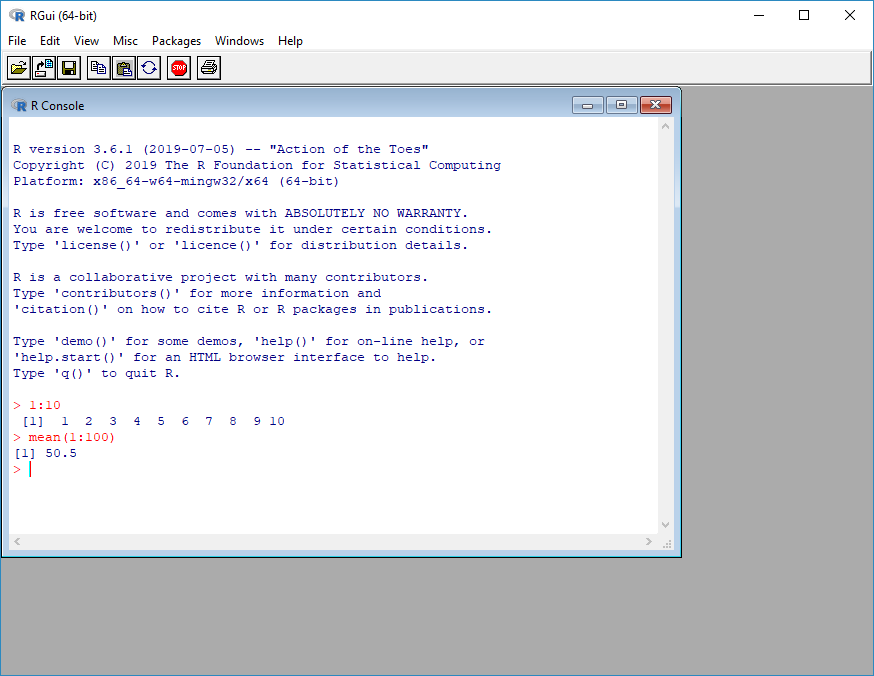
\includegraphics[width=0.7\linewidth]{images/konzol_win} }

}

\caption{RGui alkalmazás a konzollal Windows környezetben}\label{fig:konzol-win}
\end{figure}

Az \emph{RStudio} konzoljának minden korábban említett alapfunkciója az \emph{Alap R} konzoljában is elérhető, tudjuk használni a parancsok történetét, a kódkiegészítést a \texttt{TAB} billentyűvel, és a folytatás prompt (\texttt{+}) is megjelenik befejezetlen sorok esetén. Sőt a Windows alatt futó \emph{RGui} ismeri a parancsállományokat is, bár a gépeléshez korántsem kapunk annyi támogatást mint az \emph{RStudio}-ban.

\hypertarget{parancsuxe1llomuxe1nyok-az-rgui-ban}{%
\subsection{Parancsállományok az RGui-ban}\label{parancsuxe1llomuxe1nyok-az-rgui-ban}}

Az \emph{RGui} a Windows-os \emph{Alap R} része, és ahogyan láthattuk, egy nagyon egyszerű grafikus környezet, amelynek központjában a konzol található (\emph{R Console} ablak a \ref{fig:konzol-win}. ábrán). Az \emph{RGui} nagyszerű tulajdonsága, hogy támogatja a parancsállományok használatát. Az \emph{RGui}-ban találunk menüpontokat (\texttt{File/New\ script}, \texttt{File/Open\ script} és \texttt{File/Save}), amelyekkel létrehozhatunk, megnyithatunk, és elmenthetünk parancsállományokat. Tudjuk, hogy a parancsállományok használata lényegesen leegyszerűsíti az adatelemzés folyamatát, de fontos műveletként jelenik meg az átirányítás, amely a szövegszerkesztőben összegyűjtött parancsokat vezeti át a konzolba. Az \emph{RGui}-ban ez a \texttt{Ctrl+R} billentyűkombinációval lehetséges -- ez gyakorlatilag az \emph{Rstudio}-beli \texttt{Ctrl+Enter} --, de az \texttt{Edit/Run\ line\ or\ selection} vagy az \texttt{Edit/Run\ all} menüpontok is rendelkezésre állnak. A soronkénti végrehajtás mellett itt is lehetőség van kijelölt szövegrészek végrehajtására, de több sort, a teljes parancsállományt, vagy valamelyik sor egy részét is elküldhetjük a konzolba a \texttt{Ctrl+R} segítségével.

\hypertarget{r-commander}{%
\subsection{R Commander}\label{r-commander}}

Eddig az R használatának két lényegesen eltérő módját mutattuk be: a konzolos használatot és a parancsállományos használatot (az RMarkdown állományok használatát is ez utóbbi csoportba sorolhatjuk). Láttuk, hogy a konzol az \emph{RStudio} és az \emph{Alap R} központi része, de az \emph{RStudio} és az \emph{RGui} a parancsállományos használatot is támogatja. Mindegyik fenti használati mód parancsok gépelésével jár együtt.

Azonban létezik egy harmadik, az eddigiektől lényegesen eltérő módja az R használatának. Parancsok gépelése nélkül, csupán egérkattintássokkal is végezhetünk statisztikai elemzést. Az R erre alkalmas beépített eszközét \emph{R Commander}-nek nevezik, de külső eszközök is képesek az R parancssoros lényét elfedni előlünk. Ilyen külső eszköz például a \href{https://www.jamovi.org/}{\emph{jamovi}} és a \href{https://jasp-stats.org/}{\emph{JASP}}. Mindhárom felsorolt eszközben közös, hogy grafikus felhasználói felületen mozgunk, és egérkattintással, menüben való navigálással, vezérlőelemek (rádiógombok, jelölőnégyzetek, listák, nyomógombok, beviteli mezők) használatával magyarázzuk el a kívánt tevékenységet.

A továbbiakban az \emph{R Commander} lehetőségeit tekintjük át röviden. Az \emph{R Commander} az \textbf{Rcmdr} nevű csomagban foglal helyet, így használatához ezt a csomagot telepítenünk kell. Ezt követően a \texttt{library()} függvény segítségével tudjuk elindítani az \emph{R Commander}-t:

\begin{Shaded}
\begin{Highlighting}[]
\CommentTok{\# install.packages("Rcmdr")  \# R Commander telepítése}
\FunctionTok{library}\NormalTok{(Rcmdr)               }\CommentTok{\# R Commander indítása}
\end{Highlighting}
\end{Shaded}

Az indítás után egy külön \emph{R Commander} ablak jelenik meg (\ref{fig:rcommander-1}. ábra), melynek felépítése fentről lefelé a következő: (1) a gazdag menürendszer, (2) az eszköztár az aktuális adatbázis (\texttt{Adattábla}) mezővel és az \texttt{Adattábla\ megtekintése} gombokkal, (3) a parancsállomány vagy RMarkdown lapok, (4) az output számára fenntartott szöveges mező, és (5) az üzenetek helye. Megjegyezzük, hogy a \ref{fig:rcommander-1}. ábrán látható \emph{R Commander}-t az \emph{Alap R}-ből indítottuk. Amennyiben \emph{RStudio}-ból adjuk ki a \texttt{library(Rcmdr)} parancsot, akkor a 4. és az 5. elem, azaz az output és az üzenetek rész nem lesz látható, mert az \emph{RStudio} konzolja ezeket magába integrálja.

\begin{figure}

{\centering \href{}{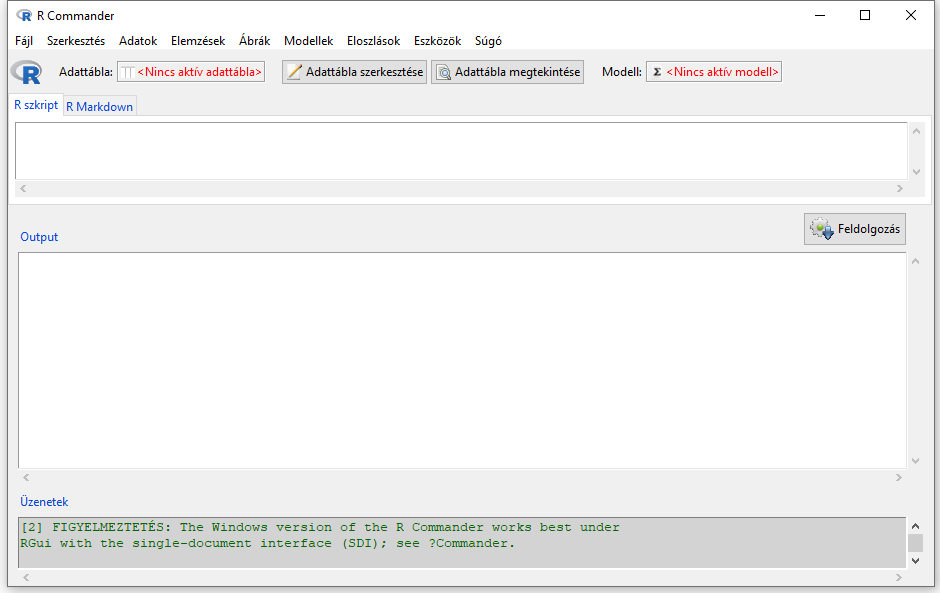
\includegraphics[width=0.85\linewidth]{images/rcommander_1} }

}

\caption{Az R Commander induló ablaka}\label{fig:rcommander-1}
\end{figure}

A kilépést az \emph{R Commander}-ből a \texttt{File\ /\ Kilépés} menüpont segítségével kezdeményezhetjük. Kilépés után az \emph{R Commander} újraindításához a következő parancsokat kell használnunk:

\begin{Shaded}
\begin{Highlighting}[]
\CommentTok{\# ha véletlenül bezártuk az R Commander{-}t}
\FunctionTok{detach}\NormalTok{(package}\SpecialCharTok{:}\NormalTok{Rcmdr)}
\FunctionTok{library}\NormalTok{(Rcmdr)}
\end{Highlighting}
\end{Shaded}

Az \emph{R Commander} lényegét a legkönnyebben úgy tudjuk szemléltetni, ha egérkattintásokkal is megoldjuk a \emph{Csillagok háborúja} c.~filmmel kapcsolatos adatelemzési feladatunkat. Első lépésként telepítsük a \textbf{dplyr} csomagot. Természetesen, ha már korábban a telepítést bármilyen apropóból elvégeztük, akkor ezt nem kell megismételni, de a teljesség kedvéért kezdjük azzal, hogyan tudunk interaktívan csomagot telepíteni az \emph{R Commander} segítségével. Válasszuk ki a \texttt{Eszközök\ /\ Csomag\ telepítése} menüpontot, ha szükséges válasszunk a tükörszerverek közül, majd válasszuk ki a megjelenő listából a \textbf{dplyr} csomagot. Ezt követően töltsük be a \textbf{dplyr} csomagot az \texttt{Eszközök\ /\ Csomag(ok)\ betöltése} menüponttal. Keressük meg a listában a \textbf{dplyr} csomagnevet és kattintsunk az \texttt{OK} gombon. Ezt követően olvassuk be a \texttt{starwars} adatbázist a \textbf{dplyr} csomagból, az \texttt{Adatok\ /\ Csomagban\ lévő\ adatok\ /\ Adattábla\ beolvasása\ betöltött\ csomagból} menüpont segítségével. Kattintsunk duplán a \textbf{dplyr} csomagneven, majd a jobb oldali listában szintén duplán a \texttt{starwars} adatbázison, majd az \texttt{OK} gombbal fejezzük be a műveletet. Figyeljük meg, hogy az \texttt{R\ szkript} és \texttt{R\ Markdown} lapok tartalmazni fogják az egérrel elmutogatott tevékenységeinknek megfelelő R parancsokat, illetve az output és üzenetek részben ezek végrehajtásáról is értesítést kapunk.

Még egy rendkívül fontos dolog történt a \textbf{dplyr} csomag \texttt{starwars} adatbázisának beolvasása után. Az eszköztárban az \texttt{Adattábla} részben már nem a \texttt{Nincs\ aktív\ adattábla} szöveg szerepel, hanem a \texttt{starwars} adatbázis neve. Azt kell megjegyeznünk az \emph{R Commander} használata során, hogy mindig van egy kitüntetett, aktív adattáblánk, és minden további tevékenység, amit a menüpontok segítségével el tudunk érni, az erre a kitüntetett, aktív adattáblára vonatkozik. Az aktív adattáblát le lehet cserélni. Amennyiben nyitnánk egy másik adatbázist, akkor a \texttt{starwars} feliratú gombon kattintva, egy listából kiválaszthatnánk, hogy melyik adatbázisunk legyen az \emph{R Commander}-ben aktív.

Folytassuk az adatelemzést az \texttt{Elemzések\ /\ Összegzések\ /\ Numerikus\ változók\ összegzése} menüpont kiválasztásával. A megjelenő dialógusdobozból válasszuk ki a \texttt{height} változót, az \texttt{Összegzés\ csoportonként} gombon kattintva pedig a \texttt{species} változót. Az \texttt{OK} gombok megnyomása után az output részben látjuk az elemzés eredményét.

Az \emph{R Commander} nagyon hatékony eszköz gyors elemzések, egyszerű adatbetekintések elvégzésére. Számos menüpontot kínál az adatok beolvasásához, előkészítéséhez és az elemzéséhez. Ráadásul az egyes menüpontokban elmutogatott tevékenységek R parancsait is szorgalmasan gyűjti, így azokat a \texttt{File\ /\ Szkript\ mentése} vagy \texttt{File\ /\ R\ Markdown\ mentése} kiválasztásával, el is tudjuk menteni magunk számára. Az \emph{R Commander} vagy a \emph{jamovi} és \emph{JASP} ismerete nagyban hozzájárul a hatékony adatelemzéshez.

Végül megemlítjük, hogy az \emph{R Commander} tudása kibővíthető beépülő modulok (plugin-ek) segítségével. Ezek új menüpontokat, dialógusdobozokat és természetesen új függvényeket tartalmaznak. A beépülő modulok csomagok formájában érhetők el. Például az \texttt{Easy\ R} beépülő modul telepítéséhez az \texttt{RcmdrPlugin.EZR} csomagra van szükség.

\begin{Shaded}
\begin{Highlighting}[]
\CommentTok{\# egy beépülő modul telepítése }
\FunctionTok{install.packages}\NormalTok{(}\StringTok{"RcmdrPlugin.EZR"}\NormalTok{)}
\end{Highlighting}
\end{Shaded}

Telepítés után a beépülő modul betöltésére is szükség van, csak így tudjuk az új funkciókat elérni. Ezt az \texttt{Eszközök\ /\ Rcmdr\ plugin(ok)\ betöltése} menüpontban tehetjük meg. Az \emph{R Commander} újraindulása után, már az új menüszerkezetet fogjuk látni. Az \href{https://socialsciences.mcmaster.ca/jfox/Misc/Rcmdr/}{\emph{R Commander hivatalos oldalán}} részletesebb információkat olvashatunk.

\hypertarget{kuxf6tegelt-futtatuxe1s}{%
\subsection{Kötegelt futtatás}\label{kuxf6tegelt-futtatuxe1s}}

Ha felidézzük az eddig tanultakat az R használati módjairól, akkor világos, hogy mindegyik az interaktív használathoz kötődik. Egy tipikus adatelemzési munka során pontosan erre van szükség: kezdeményezzük egy művelet végrehajtását és várjuk az eredményt. Újabb művelet, újabb output. Ezt a fajta interaktív használatot láttuk a konzolban, a parancsállományok és RMarkdown állományok esetén, és az \emph{R Commander}-ben is. Azonban az interaktív használat mellett beszélünk ún. kötegelt feldolgozásról is. Ez azt jelenti, hogy egy parancsállomány összes sorát egyetlen lépésben hatjuk végre. Nem vagyunk kíváncsiak a soronkénti eredményekre, a teljes szkriptállomány futtatása ad olyan eredményt, amelyre nekünk éppen szükségünk van. Kötegelt futtatásra a \texttt{source()} függvényt használhatjuk, valamint az \emph{Alap R} egy külső alkalmazását, az \texttt{Rscript} programot.

Tegyük fel, hogy egy \texttt{netflix.R} parancsállományban összegyűjtöttük az összes olyan R sort, amely egyetlen ábra létrehozásához szükséges. Ez az ábra meglehetősen összetett, mert az egyes években megjelent filmek és sorozatok számát tartalmazza, és viszonylag sok adatelőkészítési műveletet előzte meg. Ezek nem mindig izgalmasak számunkra, annál inkább maga az ábra, amelynek létrehozása a \texttt{netflix.R} egyetlen célja.

A következő sort az \emph{Alap R} vagy az \emph{RStudio} konzoljába/parancsállományába, vagy az \emph{RStudio} RMarkdown állományába is elhelyezhetjük. A \texttt{source()} függvény a \texttt{netflix.R} minden sorát végrehajtja és reményeink szerint előállítja a kívánt ábrát.

\begin{Shaded}
\begin{Highlighting}[]
\FunctionTok{source}\NormalTok{(}\StringTok{"netflix.R"}\NormalTok{, }\AttributeTok{echo =}\NormalTok{ T)}
\end{Highlighting}
\end{Shaded}

A \texttt{source()} függvény kicsit másként közelít a parancsainkhoz, mint amit megszoktunk az interaktív konzolos és parancsállományos használat során. A \texttt{source()} először a teljes állományban ellenőrzi a parancsok szintaktikai helyességét, és csak akkor kezdi el az első majd az azt követő parancsok végrehajtásához, ha mindent rendben talált.

Másik lehetőség parancsállomány kötegelt futtatására, az \texttt{RScript} program, amely ugyanúgy az \emph{Alap R} része, mint a konzol vagy az interpreter. Az operációs rendszer parancssorából kell kiadnunk a következő parancsot:

\begin{Shaded}
\begin{Highlighting}[]
\NormalTok{Rscript {-}{-}vanilla netflix.R \textgreater{} output.txt}
\end{Highlighting}
\end{Shaded}

A fenti sor hatására ugyanúgy létrejön a kívánt ábra, de az \texttt{output.txt}-ben megkapjuk a futás közben keletkező egyéb outputokat is.

Kötegelt feldolgozásra viszonylag ritkán van szükségünk, akkor is többnyire nagygépes környezetben. Az interaktív használat a legtöbb adatelemzési munka során elegendő rugalmasságot ad.

\hypertarget{munka-az-r-ben-3-summary}{%
\subsection{Összefoglalás}\label{munka-az-r-ben-3-summary}}

\begin{rmdsummary}
Amennyiben az \emph{RStudio} használatára nincs lehetőségünk, akkor az
\emph{Alap R} eszközeivel is kiválóan megoldhatjuk adatelemzési
feladatainkat. A konzol és az \emph{RGui} parancsállományai interaktív
parancsvégrehajtást biztosítanak, a \texttt{source()} függvény és az
\texttt{RScript} alkalmazás pedig a \texttt{.R} kiterjesztésű
parancsállományok kötegelt feldolgozását segítik. Az \emph{R Commander}
parancsok gépelése nélkül teszi lehetővé elemzések végrehajtását,
mindössze a megfelelő menüpontot kell kiválasztani, majd a
dialógusdobozban elvégezni a szükséges beállításokat. Érdemes kipróbálni
a \emph{jamovi} és a \emph{JASP} statisztikai programokat is.
\end{rmdsummary}

\hypertarget{munka-az-r-ben-3-exercise}{%
\subsection{Feladatok}\label{munka-az-r-ben-3-exercise}}

\begin{rmdexercise}
\begin{enumerate}
\def\labelenumi{\arabic{enumi}.}
\tightlist
\item
  Foglaljuk össze az R használati módjait! Soroljuk fel mind a négy lehetőséget!
\item
  Hasonlítsuk össze a parancsállományok használatát \emph{RGui}-ban és \emph{RStudio}-ban!
\item
  Hasonlítsuk össze a parancsállományok és az RMarkdown használatát \emph{R Commander}-ben és \emph{RStudio}-ban!
\item
  Töltsük le és telepítsük az ingyenesen elérhető \emph{jamovi} és a \emph{JASP} statisztikai programokat, majd nyissuk meg a beépített adatbázisait, és végezzünk néhány egyszerűbb elemzést! Ha elakadunk, keressünk videó tutoriált az eszközök használatáról. Melyik eszköz tetszik jobban? Miben hasonlítanak és miben térnek el?
\end{enumerate}
\end{rmdexercise}

\hypertarget{az-r-nyelv}{%
\chapter{Az R nyelv}\label{az-r-nyelv}}

\begin{center}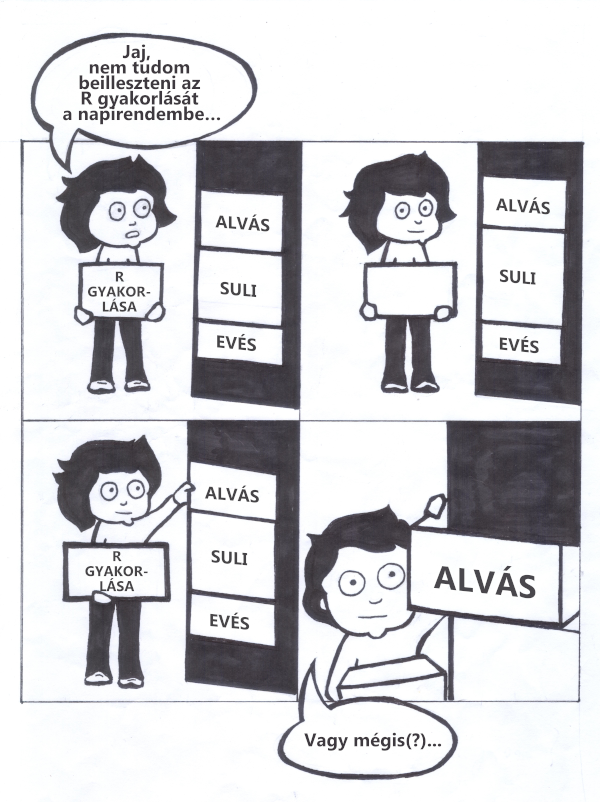
\includegraphics[width=0.7\linewidth]{images/ch_05_small} \end{center}

Az előző fejezetekben megismertük az R környezetet, az \emph{Alap R}, az \emph{RStudio} és a csomagok telepítését, megtanultuk a projektek, parancsállományok és RMarkdown állományok létrehozását. Tudjuk, a különböző környezetekben eltérő módszerekkel hajthatjuk végre az R parancsokat: a konzolban az \texttt{Enter}, a Windows-os \emph{RGui}-ban a \texttt{Ctrl+R}, míg az \emph{RStudio}-ban a \texttt{Ctrl+Enter} billentyűkombinációt kell használnunk. A parancsok végrehajtása közben érdemes észben tartani, ha a folytatás prompt (\texttt{+}) feltűnik, akkor kattintsunk bele a konzolba, és nyomjuk meg az \texttt{Esc} billentyűt, így tudunk kilépni a befejezetlen sor szerkesztéséből

E fejezet példáinak kipróbáláshoz hozzunk létre egy \texttt{gyakorlas} nevű új projektet az \emph{RStudio}-ban (\texttt{File\ /\ New\ Project}), majd készítsünk egy \texttt{gyakorlas.Rmd} RMarkdown állományt (\texttt{File\ /\ New\ File\ /\ R\ Markdown}) és egy \texttt{gyakorlas.R} parancsállományt (\texttt{File\ /\ New\ File\ /\ R\ Script}). A fejezet példáit egyaránt gépeljük az RMarkdown állomány R csonkjaiba, illetve a parancsállomány egymást követő soraiba. A fejezet további részében az R nyelvre koncentrálunk, arra, hogy mit írunk, és nem arra, hogy hová írjuk a parancsokat.

\hypertarget{adatobjektumok}{%
\section{Adatobjektumok}\label{adatobjektumok}}

\begin{rmdlevel1}
Ebben a fejezetben:

\begin{itemize}
\tightlist
\item
  áttekintjük az egyszerű számolási lehetőségeket R-ben,
\item
  bevezetjük az aritmetikai operátor és a kifejezés fogalmát,
\item
  megismerjük az objektum létrehozását és elnevezését,
\item
  több parancs elhelyezését egy sorban,
\item
  és a megjegyzések használatát.
\end{itemize}
\end{rmdlevel1}

Az R nyelv megismerését számadatok írásával kezdjük. Az adatelemzés során a számszerű adatok kezelése a leggyakoribb, hiszen méréssel és számlálással is ilyen jellegű adatokhoz jutunk. Számszerű adat a testmagasságunk cm-ben kifejezve, az IQ-teszten elért pontszámunk, vagy a testvéreink és a Facebook ismerőseink száma is.

\hypertarget{szuxe1moluxe1s-az-r-ben}{%
\subsection{Számolás az R-ben}\label{szuxe1moluxe1s-az-r-ben}}

Kezdjük a számszerű adatok megismerését egy egyszerű sor begépelésével.

\begin{Shaded}
\begin{Highlighting}[]
\DecValTok{2}\SpecialCharTok{+}\DecValTok{2} 
\CommentTok{\#\textgreater{} [1] 4}
\end{Highlighting}
\end{Shaded}

Végrehajtás után a konzolban láthatjuk az összeadás eredményét, a 4-et. Az eredmény előtt egy szögletes zárójelben lévő sorszámot is láthatunk (\texttt{{[}1{]}}), amely bonyolultabb outputokban segít eligazodni. Később az \ref{szabalyosvektorokalfejezet}. fejezetben visszatérünk a \texttt{{[}1{]}} értelmezésére.

Látjuk, ebben az esetben az R úgy viselkedik, mint egy számológép. Kiszámolja a parancssorba gépelt algebrai kifejezés értékét, majd a képernyőn megjeleníti. Természetesen az összeadáson túl más műveletet is használhatunk.

\begin{Shaded}
\begin{Highlighting}[]
\DecValTok{4}\SpecialCharTok{+}\DecValTok{6}\SpecialCharTok{*}\DecValTok{2}
\CommentTok{\#\textgreater{} [1] 16}
\end{Highlighting}
\end{Shaded}

A fenti példából látható, hogy az R követi a műveletek elvégzésének matematikában megszokott sorrendjét. Azaz a szorzás műveletre (\texttt{*}) hamarabb sor kerül, ennek eredménye 12. Ezt követi az összeadás (\texttt{+}), most már a 4 és a 12 között. Ennek az összeadás műveletnek az eredménye 16, ami egyben a kifejezés értéke is, tehát ez jelenik meg a konzolban.

Természetesen a matematikában megszokott módon változtathatunk a műveletek végrehajtásának alapértelmezett sorrendjén, azaz használhatunk kerek zárójeleket. Ezeket az R a megszokott módon értelmezi: a zárójelben szereplő műveletek végrehajtását előreveszi.

\begin{Shaded}
\begin{Highlighting}[]
\NormalTok{(}\DecValTok{4}\SpecialCharTok{+}\DecValTok{6}\NormalTok{)}\SpecialCharTok{*}\DecValTok{2}
\CommentTok{\#\textgreater{} [1] 20}
\end{Highlighting}
\end{Shaded}

A fenti példában az összeadás művelet lesz az első, amelynek az eredménye 10. Ezt követi a szorzás, így kapjuk a kifejezés értékeként a 20-at.

Ezeket a matematikában megszokott algebrai kifejezéseket, az R-ben egyszerűen kifejezésnek vagy -- utalva arra, hogy a kifejezés értéke szám -- \emph{aritmetikai kifejezésnek}\index{aritmetikai kifejezés} nevezünk. Az eddigiek alapján az aritmetikai kifejezések tehát a következő nyelvi elemeket tartalmazhatják:

\begin{itemize}
\tightlist
\item
  számok, amelyeket \emph{numerikus konstans}oknak\index{numerikus konstans} nevezünk,
\item
  műveleti jelek, amelyeket \emph{aritmetikai operátor}oknak\index{aritmetikai operátor} nevezünk,
\item
  és kerek zárójelek.
\end{itemize}

A fentiek alapján összetettebb aritmetikai kifejezéseket is megformálhatunk. Az R minden esetben kiszámolja a kifejezések értékét -- azaz \emph{kiértékeli} a kifejezést --, és a kapott értéket megjeleníti a konzolban.

\begin{Shaded}
\begin{Highlighting}[]
\DecValTok{4}\SpecialCharTok{\^{}}\DecValTok{2{-}3}\SpecialCharTok{*}\DecValTok{2}\SpecialCharTok{+}\DecValTok{1}
\CommentTok{\#\textgreater{} [1] 11}
\NormalTok{(}\DecValTok{104{-}20}\NormalTok{)}\SpecialCharTok{/}\DecValTok{6{-}4}\SpecialCharTok{*}\DecValTok{7}\SpecialCharTok{*}\DecValTok{10}\SpecialCharTok{/}\NormalTok{(}\DecValTok{5}\SpecialCharTok{**}\DecValTok{2{-}5}\NormalTok{)}
\CommentTok{\#\textgreater{} [1] 0}
\end{Highlighting}
\end{Shaded}

\begin{table}

\caption{\label{tab:matoperatorok}Matematikai operátorok precedenciájuk csökkenő sorrendjében}
\centering
\begin{tabular}[t]{lll}
\toprule
Operátor & Művelet & Példa\\
\midrule
\cellcolor{gray!6}{\ttfamily{\textasciicircum{} **}} & \cellcolor{gray!6}{hatványozás} & \cellcolor{gray!6}{\ttfamily{2\textasciicircum{}3;2**3}}\\
\ttfamily{+ - } & előjelek & \ttfamily{+3.3;-.5}\\
\cellcolor{gray!6}{\ttfamily{\%\% \%/\%}} & \cellcolor{gray!6}{maradékos osztás és egész osztás} & \cellcolor{gray!6}{\ttfamily{13\%\%4;15\%/\%4}}\\
\ttfamily{* /} & szorzás és osztás & \ttfamily{2*3;4/2}\\
\cellcolor{gray!6}{\ttfamily{+ - }} & \cellcolor{gray!6}{összeadás és kivonás} & \cellcolor{gray!6}{\ttfamily{2+3;2-3}}\\
\bottomrule
\end{tabular}
\end{table}

Az aritmetikai kifejezések használata során ne felejtkezzünk el a műveletek alapértelmezett végrehajtási sorrendjéről. A műveletek megjelenítését most az operátorok végzik, melyeknek fontos tulajdonsága, hogy mennyire szorosan kötik magukhoz az adatokat (vagy más néven az operandusokat). Az operátorok ezen fonos tulajdonságát \emph{precedenciának} nevezzük. Az R-ben használható aritmetikai operátorokat a precedenciájuk csökkenő sorrendjében az \ref{tab:matoperatorok}. táblázat tartalmazza.

Például a hatványozás és az előjel operátor precedenciája eltér egymástól, a hatványozás nagyobb precedenciájú, azaz szorosabban köti magához az adatokat, így végrehajtása megelőzi az előjel operátort. Ha nem vagyunk elég óvatosak, és plusz zárójelek segítségével nem biztosítjuk a kívánt végrehajtási sorrendet, akkor ``váratlan'' eredményhez juthatunk. A lenti példában láthatjuk, hogy zárójelek nélkül a nagyobb precedenciájú hatványozás az elsőként végrehajtott művelet.

\begin{Shaded}
\begin{Highlighting}[]
\SpecialCharTok{{-}}\DecValTok{2}\SpecialCharTok{\^{}}\DecValTok{2}    \CommentTok{\# először hatványozás, majd előjel}
\CommentTok{\#\textgreater{} [1] {-}4}
\NormalTok{(}\SpecialCharTok{{-}}\DecValTok{2}\NormalTok{)}\SpecialCharTok{\^{}}\DecValTok{2}  \CommentTok{\# először előjel, majd hatványozás}
\CommentTok{\#\textgreater{} [1] 4}
\end{Highlighting}
\end{Shaded}

Eddig láthattuk, hogy kifejezéseinket operátorok, numerikus konstansok és zárójelek segítségével építettük fel. Ezek a kifejezések két alkotójukban is általánosíthatók:

\begin{itemize}
\tightlist
\item
  általánosítható a kifejezés adat része, amelyet eddig a numerikus konstansok képviseltek (ezekből lesznek az \emph{objektum}ok),
\item
  általánosíthatő a kifejezés művelet része, amelyet eddig az operátorok jelenítettek meg (ezek lesznek a \emph{függvény}ek).
\end{itemize}

Az adatrész általánosítása tehát az adatobjektum (vagy röviden objektum), a műveleteké pedig a függvényobjektum (vagy röviden függvény). Ezeket tekintjük át a következőkben.

\hypertarget{objektumok}{%
\subsection{Objektumok}\label{objektumok}}

Ha egy kifejezés értéket nem egyszerűen a képernyőn szeretnénk megjeleníteni, hanem azt később is fel szeretnénk használni, akkor objektumot\footnote{Más programozási nyelvekben az ``objektum'' helyett a ``változó'' elnevezést használják, de a változó fogalma már foglalt a statisztikában, így szerencsésebb a memóriában tárolt adatokra objektumként hivatkozni.} kell létrehoznunk. Az objektumok révén a memóriába rögzíthetünk tetszőleges értékeket, később pedig elővehetjük és felhasználhatjuk ezeket az értékeket.
Tudjuk, ha a lenti aritmetikai kifejezést a parancssorba írjuk, az R miután kiértékelte a kifejezést, a kifejezés értékét megjeleníti a konzolban. Ez az érték azonban a megjelenítés után rögtön el is vész, többször nem használhatjuk fel.

\begin{Shaded}
\begin{Highlighting}[]
\DecValTok{1157}\SpecialCharTok{/}\DecValTok{13}\SpecialCharTok{+}\DecValTok{2}\SpecialCharTok{\^{}}\DecValTok{3} 
\CommentTok{\#\textgreater{} [1] 97}
\end{Highlighting}
\end{Shaded}

Ha létrehozunk egy \texttt{x} nevű objektumot, akkor ezt az értéket további kifejezésekben is szerepeltethetjük. Minden olyan helyen, ahol eddig számok jelentek meg a kifejezésekben, oda ez az \texttt{x} objektumnév is beírható.

\begin{Shaded}
\begin{Highlighting}[]
\NormalTok{x }\OtherTok{\textless{}{-}} \DecValTok{1157}\SpecialCharTok{/}\DecValTok{13}\SpecialCharTok{+}\DecValTok{2}\SpecialCharTok{\^{}}\DecValTok{3} 
\end{Highlighting}
\end{Shaded}

A fenti sor végrehajtása után írhatjuk a következőket, hiszen a kifejezések kiértékelése során az \texttt{x} objektum memóriában tárolt értékével fog számolni az R.

\begin{Shaded}
\begin{Highlighting}[]
\NormalTok{x}\SpecialCharTok{+}\DecValTok{2}       \CommentTok{\# mintha 97+2 lenne}
\CommentTok{\#\textgreater{} [1] 99}
\DecValTok{2}\SpecialCharTok{*}\NormalTok{x}\SpecialCharTok{\^{}}\DecValTok{3}\SpecialCharTok{+}\DecValTok{5}   \CommentTok{\# 2*97\^{}3+5}
\CommentTok{\#\textgreater{} [1] 1825351}
\end{Highlighting}
\end{Shaded}

Minden objektumnak van neve és tartozik hozzá a memóriában egy terület, ahol a kérdéses érték tárolásra kerül. Esetünkben az objektum neve \texttt{x}, a hozzá tartozó memóriaterületen pedig a 97 értéket tárolja az R. Az objektum leegyszerűsítve tehát egy név-érték pár, ahol a nevet és a memóriában eltárolandó értéket is mi magunk választjuk meg.

Az objektumok kezeléséhez 3 művelet kapcsolódik:

\begin{itemize}
\tightlist
\item
  objektum létrehozása,
\item
  objektum értékének lekérdezése,
\item
  és az objektum értékének megváltoztatása.
\end{itemize}

\hypertarget{objektumok-luxe9trehozuxe1sa}{%
\subsubsection{Objektumok létrehozása}\label{objektumok-luxe9trehozuxe1sa}}

Objektumot értékadással hozhatunk létre. Az értékadás tartalmaz egy értékadás operátort, melynek alakja \texttt{\textless{}-} (balra nyíl), vagyis egy kisebb jel és egy mínusz előjel egymás után írva szóköz nélkül\footnote{További értékadás operátorok a \texttt{-\textgreater{}}, \texttt{\textless{}\textless{}-}, \texttt{-\textgreater{}\textgreater{}} és a \texttt{=}. Ezeket nem használjuk ebben a könyvben.}.

Az értékadás általános alakja:

\begin{Shaded}
\begin{Highlighting}[]
\NormalTok{objektumnév \textless{}{-} kifejezés    \# értékadó utasítás}
\end{Highlighting}
\end{Shaded}

Ahol lehet a továbbiakban ezt a balra nyíl alakú értékadó operátort használjuk az értékadás során, és nem a szintén legális egyenlőségjelet (\texttt{=}). A balra nyíl írását az \emph{RStudio} az \texttt{Alt+-} segítségével támogatja, így a bevitele nem okozhat nehézséget. Az egyenlőségjelet megtartjuk a függvényargumentumok elnevezésére. Az egyszerűség kedvéért a balra nyíl előtt lévő objektumnevet az értékadás bal oldalának, az utána lévő kifejezést az értékadás jobb oldalának nevezzük.

Ha olyan objektumnevet szerepeltetünk az értékadásban, amely még nem létezik, akkor az R létrehoz egy ilyen nevű új objektumot, és a hozzá tartozó memóriaterületen pedig az értékadás jobb oldalán lévő kifejezés kiértékelése után kapott értéket tárolja el.

\begin{Shaded}
\begin{Highlighting}[]
\NormalTok{a }\OtherTok{\textless{}{-}} \DecValTok{1}\SpecialCharTok{+}\DecValTok{2}    \CommentTok{\# objektum létrehozása}
\end{Highlighting}
\end{Shaded}

A fenti sor végrehajtása után a konzolban nem jelenik meg eredmény, mégis egy nagyon fontos dolog történik, létrejön az \texttt{a} nevű objektum, amelynek értéke 3 lesz mindaddig, amig ezen nem változtatunk. A munkánk során létrehozott objektumok a memória egy speciális területére, a \emph{munkaterület}re (\emph{workspace}) kerülnek.

Ha az értékadásban használt objektum már létezik, akkor a jobb oldali kifejezés kiértékelése után a kapott értékkel felülírja a bal oldali objektumhoz tartozó memóriaterületet. Ezzel a módszerrel tehát a korábban létrehozott objektum értékét módosíthatjuk.

A már létező \texttt{a} objektum értékét könnyen megváltoztathatjuk.

\begin{Shaded}
\begin{Highlighting}[]
\NormalTok{a }\OtherTok{\textless{}{-}} \DecValTok{10}\SpecialCharTok{/}\DecValTok{3}   \CommentTok{\# objektum értékének megváltoztatása}
\end{Highlighting}
\end{Shaded}

\hypertarget{objektumok-uxe9rtuxe9kuxe9nek-lekuxe9rdezuxe9se}{%
\subsubsection{Objektumok értékének lekérdezése}\label{objektumok-uxe9rtuxe9kuxe9nek-lekuxe9rdezuxe9se}}

Az objektum memóriában tárolt értékét le is kérdezhetjük. A legegyszerűbb mód erre, ha az objektum nevét a parancssorba írjuk és végrehajtjuk a sort, máris megkapjuk az objektum memóriában tárolt értékét.

\begin{Shaded}
\begin{Highlighting}[]
\NormalTok{a     }\CommentTok{\# vajon mi az "a" objektum értéke}
\CommentTok{\#\textgreater{} [1] 3.333}
\end{Highlighting}
\end{Shaded}

Objektumok tetszőleges kifejezésben megjelenhetnek, akár egy értékadás jobb oldalán lévő kifejezésben is. A kifejezések kiértékelésében az objektum a memóriában tárolt értékével vesz részt.

\begin{Shaded}
\begin{Highlighting}[]
\NormalTok{a}\SpecialCharTok{*}\DecValTok{3}              \CommentTok{\# a kifejezés értéke konzolba kerül}
\CommentTok{\#\textgreater{} [1] 10}
\NormalTok{a }\OtherTok{\textless{}{-}} \DecValTok{4} \SpecialCharTok{+}\NormalTok{ a }\SpecialCharTok{*} \DecValTok{3}   \CommentTok{\# megváltozik az objektum értéke, nincs output}
\NormalTok{a                }\CommentTok{\# megtudjuk az objektum értékét}
\CommentTok{\#\textgreater{} [1] 14}
\end{Highlighting}
\end{Shaded}

A fenti sorokból kiolvasható, hogy immár az \texttt{a} objektum értéke 14.

\hypertarget{objektumelnevezes}{%
\subsubsection{Objektumok elnevezése}\label{objektumelnevezes}}

Az objektumok elnevezésére eddig egyetlen betűt (karaktert) használtunk, de ez elég ritka eset a munka során. Helyes gyakorlat, ha az objektum neve utal az objektum tartalmára, céljára. Ha például testmagasságot tárolunk el egy objektumban, akkor írhatjuk a következőt:

\begin{Shaded}
\begin{Highlighting}[]
\NormalTok{magassag }\OtherTok{\textless{}{-}} \DecValTok{179}
\end{Highlighting}
\end{Shaded}

A fenti sor létrehozza a munkaterületen a \texttt{magassag} nevű objektumot 179 értékkel.

Az objektumok elnevezésére

\begin{itemize}
\tightlist
\item
  betűket,
\item
  számjegyeket,
\item
  és az aláhúzás (\texttt{\_}) vagy pont (\texttt{.}) szimbólumokat használhatjuk.
\end{itemize}

Az objektum neve csak betűvel vagy ponttal kezdődhet, számjeggyel vagy aláhúzással nem. Továbbá a név nem lehet az R-ben már lefoglalt kulcsszó, mint például \texttt{if}, \texttt{function} vagy \texttt{TRUE} (a kulcsszavak listáját a \texttt{?Reserved} paranccsal ismerhetjük meg). Hagyományosan a pont karaktert használjuk az objektumnevekben a tagolásra (például \texttt{magassag.peter} Péter magasságának tárolására). Az R a magyar ékezetes karakterek használatát is megengedi az objektumnevekben, de csakúgy mint az állományok és könyvtárak elnevezésében, érdemes ezek használatát mellőzni.

Az objektumoknak érdemes ``beszédes'' nevet választani, még ha ennek az ára némi extra gépelés is. Tudjuk, a \texttt{Tab} billentyű segíti a gépelést az \emph{RStudio}-ban.

Az R kis- és nagybetű érzékeny, vagyis az \texttt{x} és a \texttt{X} különböző objektumoknak számítanak. Például a következő

\begin{Shaded}
\begin{Highlighting}[]
\NormalTok{pulzus.atlag }\OtherTok{\textless{}{-}} \DecValTok{72}
\end{Highlighting}
\end{Shaded}

parancs után a

\begin{Shaded}
\begin{Highlighting}[]
\NormalTok{Pulzus.atlag}
\CommentTok{\#\textgreater{} Error: object \textquotesingle{}Pulzus.atlag\textquotesingle{} not found}
\end{Highlighting}
\end{Shaded}

sor hibát jelez (\texttt{Error:\ object\ \textquotesingle{}Pulzus.atlag\textquotesingle{}\ not\ found}), azaz a \texttt{Pulzus.atlag} objektumot nem találja az R. Minden olyan esetben, ha nem létező objektumra hivatkozunk, a fenti hibaüzenet jelenik meg a konzolban.

Amennyiben gondoskodunk nagy \texttt{P}-vel kezdődő objektumról is, akkor lehetőségünk van hibaüzenet nélkül mindkét objektum értékének kiíratására.

\begin{Shaded}
\begin{Highlighting}[]
\NormalTok{Pulzus.atlag }\OtherTok{\textless{}{-}} \DecValTok{69}           \CommentTok{\# új objektumot hozunk létre}
\NormalTok{Pulzus.atlag; pulzus.atlag   }\CommentTok{\# két parancs egy sorban}
\CommentTok{\#\textgreater{} [1] 69}
\CommentTok{\#\textgreater{} [1] 72}
\end{Highlighting}
\end{Shaded}

A gyakorlatban kerüljük el az olyan helyzeteket, amikor két objektumnév csak kis- nagybetűk használatában tér el.

A fenti példában egy további apró újdonság is szerepelt. Ha egy parancssorban több utasítást szeretnénk elhelyezni, akkor ezeket pontosvesszővel (\texttt{;}) kell elválasztanunk. A pontosvesszővel elválasztott utasításokat az R értelmező egymás után, balról jobbra haladva hajtja végre, mintha külön sorba írtuk volna őket. A lenti sor 3 kifejezést (parancsot) tartalmaz pontosvesszővel elválasztva, mindegyik eredménye külön-külön jelenik meg a konzolban, mintha 3 különböző sorba írtuk volna őket.

\begin{Shaded}
\begin{Highlighting}[]
\DecValTok{1}\SpecialCharTok{+}\DecValTok{2}\NormalTok{; }\DecValTok{3}\SpecialCharTok{+}\DecValTok{4}\NormalTok{; }\DecValTok{5}\SpecialCharTok{+}\DecValTok{6}     \CommentTok{\# három kifejezés egy sorban}
\CommentTok{\#\textgreater{} [1] 3}
\CommentTok{\#\textgreater{} [1] 7}
\CommentTok{\#\textgreater{} [1] 11}
\end{Highlighting}
\end{Shaded}

\hypertarget{MegjegyzesazRben}{%
\subsection{Megjegyzések}\label{MegjegyzesazRben}}

Nagyon sok példában láttunk már magyar nyelvű, magyarázó, értelmező szövegrészeket az R parancsok körül. Ezek az R \emph{megjegyzések}. Megjegyzést az R-ben a kettőskereszt (\texttt{\#}) karakter használatával vezetünk be. Az R értelmező a kettőskereszttől a sor végéig tartó részt figyelmen kívül hagyja. Itt helyezhetjük el a paranccsal kapcsolatos magyarázatainkat magunk vagy a kódot később olvasók számára. Teljes sorokat, vagy a sorok végét tudjuk így kivonni a végrehajtás alól.

\begin{Shaded}
\begin{Highlighting}[]
\CommentTok{\# Érdekes tény, ha a 153 számjegyeit köbre emeljük, }
\CommentTok{\#   majd összeadjuk őket, pontosan 153{-}at kapunk}
\DecValTok{1}\SpecialCharTok{\^{}}\DecValTok{3}\SpecialCharTok{+}\DecValTok{5}\SpecialCharTok{\^{}}\DecValTok{3}\SpecialCharTok{+}\DecValTok{3}\SpecialCharTok{\^{}}\DecValTok{3}       \CommentTok{\# hatványozás a \^{} operátorral}
\CommentTok{\#\textgreater{} [1] 153}
\DecValTok{1}\SpecialCharTok{**}\DecValTok{3}\SpecialCharTok{+}\DecValTok{5}\SpecialCharTok{**}\DecValTok{3}\SpecialCharTok{+}\DecValTok{3}\SpecialCharTok{**}\DecValTok{3}    \CommentTok{\# hatványozás a ** operátorral}
\CommentTok{\#\textgreater{} [1] 153}
\end{Highlighting}
\end{Shaded}

Nem kizárólag magyarázó szövegek kerülhetnek megjegyzésbe, sokszor R parancsok végrehajtását akadályozzuk meg ezzel a módszerrel. Úgy kerülhetjük el egy parancs végrehajtását, hogy nem kell kitörölnünk a parancsállományból vagy az RMarkdown állományból, egyszerűen csak megjegyzésbe kell tennünk őket. Emlékezzünk vissza, hogy az \ref{Csomagoktelepitese}. fejezetben a csomagok telepítésért felelős parancsok esetében kifezetten javasoltuk a megjegyzések használatát:

\begin{Shaded}
\begin{Highlighting}[]
\CommentTok{\# xkcd: Randall Munroe webképregényei}
\CommentTok{\# install.packages("RXKCD")}
\FunctionTok{library}\NormalTok{(RXKCD)             }\CommentTok{\# csomag betöltése       }
\FunctionTok{searchXKCD}\NormalTok{(}\StringTok{"Star Wars"}\NormalTok{)    }\CommentTok{\# keresés címben vagy leírásban}
\FunctionTok{getXKCD}\NormalTok{(}\DecValTok{1769}\NormalTok{)              }\CommentTok{\# webképregény megjelenítése}
\end{Highlighting}
\end{Shaded}

Végül megemlítjük, hogy az \emph{RStudio}-ban egyszerre több kijelölt sort tudunk megjegyzésbe tenni, vagy onnan kivenni a \texttt{Ctrl+Shift+C} segítségével.

\hypertarget{az-r-nyelv-1-summary}{%
\subsection{Összefoglalás}\label{az-r-nyelv-1-summary}}

\begin{rmdsummary}
Egyszerű kifejezéseket építhetünk numerikus konstansok (számok),
operátorok és kerek zárójelek segítségével. A legfontosabb matematikai
operátorok a négy alapművelet és a hatványozás. A kifejezés kiértékelése
balról jobbra sorrendben történik, de ezt felülírhatja a kerek zárójelek
használata és az operátorok precedenciája. Egy kifejezés értékét
eltárolhatjuk a memória speciális területén, a munkamemóriában. Ehhez az
értékadó operátorral (\texttt{\textless{}-}) létre kell hoznunk egy új
objektumot. Az objektum egy név-érték páros. Az objektum létrehozása
után az objektum neve megjelenhet egy tetszőleges kifejezés adat
részében. Több parancsot a pontosvesszővel (\texttt{;}) írhatunk egy
sorba. Megjegyzéseket a kettőskereszt (\texttt{\#}) segítségével
helyezhetünk el.
\end{rmdsummary}

\hypertarget{az-r-nyelv-1-exercise}{%
\subsection{Feladatok}\label{az-r-nyelv-1-exercise}}

\begin{rmdexercise}
\begin{enumerate}
\def\labelenumi{\arabic{enumi}.}
\tightlist
\item
  Gondoljuk át, mi lehet a következő algebrai kifejezés eredménye, majd ellenőrizzük R-ben is: \(8/2(2+2)\).
\item
  Gondoljuk át, hogy a \texttt{.342e1} név miért nem lehet érvényes objektumnév? Próbáljuk ki a \texttt{make.names(".342e1")} parancsot, majd tanulmányozzuk a \texttt{?make.names} leírást!
\item
  Magyarázzuk meg a \texttt{make.names(c("",\ "",\ ""))} és a \texttt{make.names(c("",\ "",\ ""),\ unique\ =\ T)} parancsok közötti különbséget!
\item
  Gondoljuk át, hogy egy parancsállomány mely pontjain érdemes feltétlenül megjegyzéseket használni!
\item
  Jelentősen segíthetjük a navigációt az \emph{RStudio} parancsállományaiban, ha bizonyos megjegyzések végére ezt írjuk: \texttt{-\/-\/-\/-} (szóköz és négy mínusz jel). Hogyan használhatjuk ezt a lehetőséget az \emph{RStudio}-ban, és milyen előnyei vannak?
\item
  Az \emph{RStudio}-ban parancsállomány (\texttt{.R}) szerkesztése közben próbáljuk ki a \texttt{Ctrl+Alt+R} billentyűparancsot, és a hozzá kapcsolódó \texttt{Shift+Alt+J} billentyűparancsot is. Mi a jelentése az \texttt{Alt+L}, \texttt{Shift+Alt+L}, \texttt{Alt+O} és \texttt{Shift+Alt+O} billentyűparancsoknak? A most megismert funkciók hogyan válthatók ki RMarkdown (\texttt{.Rmd}) állomány szerkesztése közben?
\end{enumerate}
\end{rmdexercise}

\hypertarget{fuxfcggvuxe9nyek}{%
\section{Függvények}\label{fuxfcggvuxe9nyek}}

\begin{rmdlevel1}
Ebben a fejezetben:

\begin{itemize}
\tightlist
\item
  áttekintjük a függvényhívás lehetőségeit a nevesített argumentumokkal, az alapértelmezésekkel és az argumentumok sorrendjének megváltoztatásával,
\item
  megismerjük a legfontosabb matematikai függvényeket,
\item
  és pontosítjuk a kifejezés fogalmát.
\end{itemize}
\end{rmdlevel1}

Az aritmetikai kifejezéseinkben használható operátorok nem teszik lehetővé minden matematikai művelet elvégzését. Mit tegyünk ha a 2 négyzetgyökét szeretnénk kiszámolni? A négyzetgyökvonás operátor nem létezik az R-ben, de ebben a speciális esetben a hatványozás operátor segítségével is elérhetjük a célunkat.

\begin{Shaded}
\begin{Highlighting}[]
\DecValTok{2}\SpecialCharTok{\^{}}\FloatTok{0.5}
\CommentTok{\#\textgreater{} [1] 1.414}
\end{Highlighting}
\end{Shaded}

Az R azonban más lehetőséget is biztosít a négyzetgyök kiszámítására és ez az \texttt{sqrt()} függvény.

\begin{Shaded}
\begin{Highlighting}[]
\FunctionTok{sqrt}\NormalTok{(}\DecValTok{2}\NormalTok{)}
\CommentTok{\#\textgreater{} [1] 1.414}
\end{Highlighting}
\end{Shaded}

A függvények valamilyen utasítássorozatot hajtanak végre és a számítás eredményét szolgáltatják. Esetünkben az \texttt{sqrt()} függvény egy szám (pozitív) négyzetgyökét számolja ki, annak a számnak a négyzetgyökét, amely a kerek zárójelek között szerepel. Tehát az R a paraméterben megadott 2 értékre meghívja az \texttt{sqrt()} függvényt, ami visszatér a 2 négyzetgyökével.

\hypertarget{a-fuxfcggvuxe9nyhuxedvuxe1s-szabuxe1lyai}{%
\subsection{A függvényhívás szabályai}\label{a-fuxfcggvuxe9nyhuxedvuxe1s-szabuxe1lyai}}

A függvényhívás általános alakja:

\begin{Shaded}
\begin{Highlighting}[]
\NormalTok{függvénynév(argNév1=arg1, argNév2=arg2, ..., argNévN=argN)}
\end{Highlighting}
\end{Shaded}

A függvény neve ugyanazoknak a szabályoknak engedelmeskedik, amelyeket az objektumok nevénél megtárgyaltunk (lévén a függvény is egy objektum). A függvény neve után kerek zárójelben következnek a függvény argumentumai, amelyek a függvény utasításainak a bemenő paraméterei. A függvény a bemenő paraméterek alapján az utasításainak megfelelően egy visszatérési értéket fog szolgáltatni.

Egy függvény különböző hívásainál az előforduló argumentumok száma és azok sorrendje igen változatos képet mutathat. Elöljáróban elmondhatjuk, hogy a függvények argumentumai alapértelmezett értékkel is rendelkezhetnek, így ezek az argumentumok elhagyhatók. Továbbá, a függvények argumentumai névvel is rendelkeznek, amelyeket ha a függvény hívásánál felhasználjuk, az argumentumok sorrendje tetszőleges lehet.

Először tekintsük át az R alapvető matematikai függvényeit (\ref{tab:matfuggvenyek}. táblázat). Nézzük meg részletesebben a \texttt{log()} függvényt. Ha kikérjük a súgóját a \texttt{?log} parancs begépelésével, akkor megtudhatjuk, hogy ez a legáltalánosabb logaritmus függvény, tetszőleges alap esetén hívható. Számunkra most a legfontosabb a súgónak az a sora, amely a logaritmus függvény használatát mutatja: \texttt{log(x,\ base=exp(1))}.

\begin{table}

\caption{\label{tab:matfuggvenyek}Az R alapvető matematikai függvényei}
\centering
\resizebox{\linewidth}{!}{
\begin{tabular}[t]{lll}
\toprule
Függvény & Leírás & Példa\\
\midrule
\cellcolor{gray!6}{\ttfamily{abs(x)}} & \cellcolor{gray!6}{abszolútérték függvény} & \cellcolor{gray!6}{\ttfamily{abs(-1)}}\\
\ttfamily{sign(x)} & előjel függvény & \ttfamily{sign(pi)}\\
\cellcolor{gray!6}{\ttfamily{sqrt(x)}} & \cellcolor{gray!6}{négyzetgyök függvény} & \cellcolor{gray!6}{\ttfamily{sqrt(9+16)}}\\
\ttfamily{exp(x)} & exponenciális függvény & \ttfamily{exp(1)}\\
\cellcolor{gray!6}{\ttfamily{log(x,base=exp(1))}} & \cellcolor{gray!6}{logaritmus függvény} & \cellcolor{gray!6}{\ttfamily{log(exp(3));log(8,10)}}\\
\addlinespace
\ttfamily{log10(x);log2(x)} & 10-es és 2-es alapú logaritmus & \ttfamily{log10(1000);log2(256)}\\
\cellcolor{gray!6}{\ttfamily{cos(x);sin(x);tan(x)}} & \cellcolor{gray!6}{trigonometrikus függvények} & \cellcolor{gray!6}{\ttfamily{cos(pi);sin(0);tan(0)}}\\
\ttfamily{round(x,digits=0)} & kerekítés adott tizedesre & \ttfamily{round(c(1.5,-1.5))}\\
\cellcolor{gray!6}{\ttfamily{floor(x)}} & \cellcolor{gray!6}{x-nél kisebb, legnagyobb egész} & \cellcolor{gray!6}{\ttfamily{floor(c(1.5,-1.5))}}\\
\ttfamily{ceiling(x)} & x-nél nagyobb, legkisebb egész & \ttfamily{ceiling(c(1.5,-1.5))}\\
\addlinespace
\cellcolor{gray!6}{\ttfamily{trunc(x)}} & \cellcolor{gray!6}{x-hez közelebbi egész x és 0 között} & \cellcolor{gray!6}{\ttfamily{trunc(c(1.5,-1.5))}}\\
\bottomrule
\end{tabular}}
\end{table}

Ebből kiolvasható, hogy a \texttt{log()} függvénynek 2 argumentuma (más néven paramétere) van. Az elsőt \texttt{x}-nek, a másodikat \texttt{base}-nek nevezik. A második paraméter alapértelmezett értékkel is rendelkezik, tehát ez a paraméter a hívásnál elhagyható, míg az \texttt{x=} argumentum megadása kötelező. A \texttt{base=} paraméter értéke könnyen kideríthető az

\begin{Shaded}
\begin{Highlighting}[]
\FunctionTok{exp}\NormalTok{(}\DecValTok{1}\NormalTok{)    }\CommentTok{\#  Euler{-}féle szám, a természetes logaritmus alapja }
\CommentTok{\#\textgreater{} [1] 2.718}
\end{Highlighting}
\end{Shaded}

parancsból. Ezt az irracionális számot a matematikában \emph{e}-vel jelöljük, és Euler-féle számnak nevezzük, ez a természetes logaritmus alapja. Ha nem határozzuk meg a második paramétert, akkor a \texttt{log()} függvény ezzel a természetes alappal (\texttt{base=exp(1)}) számítja ki az \texttt{x} logaritmusát.

Ezek alapján 2 természetes alapú logaritmusát a

\begin{Shaded}
\begin{Highlighting}[]
\FunctionTok{log}\NormalTok{(}\DecValTok{2}\NormalTok{)    }\CommentTok{\# 2 természetes alapú logaritmusa}
\CommentTok{\#\textgreater{} [1] 0.6931}
\end{Highlighting}
\end{Shaded}

függvényhívás adja meg. Azt is megtehetjük, hogy felhasználjuk hívásnál az argumentum nevét (\texttt{x}), és egy egyenlőségjel (\texttt{=}) felhasználásával ezt a 2 elé szúrjuk be.

\begin{Shaded}
\begin{Highlighting}[]
\FunctionTok{log}\NormalTok{(}\AttributeTok{x=}\DecValTok{2}\NormalTok{)   }\CommentTok{\# 2 természetes alapú logaritmusa}
\CommentTok{\#\textgreater{} [1] 0.6931}
\end{Highlighting}
\end{Shaded}

A fenti sor természetesen ugyanúgy a 2 természetes alapú logaritmusát szolgáltatja, csak most explicit módon közöltük, hogy az aktuális paraméterben szereplő 2-es értéket az \texttt{x=} nevű formális paraméternek feleltetjük meg. Ez most felesleges gépelést jelentett és általában is elmondhatjuk, hogy matematikai függvények esetében az oly gyakori \texttt{x=} argumentumnevet szokás szerint nem írjuk ki a függvényhívás során.

Hívjuk most két argumentummal a \texttt{log()} függvényt. A 100 10-es alapú logaritmusát a

\begin{Shaded}
\begin{Highlighting}[]
\FunctionTok{log}\NormalTok{(}\DecValTok{100}\NormalTok{, }\DecValTok{10}\NormalTok{)        }\CommentTok{\# 100 10{-}es alapú logaritmusa}
\CommentTok{\#\textgreater{} [1] 2}
\end{Highlighting}
\end{Shaded}

paranccsal tudhatjuk meg. A függvényhívásnál az \texttt{x=} formális argumentum a 100, a \texttt{base=} pedig a 10 értéket kapja. Természetesen ezt a hívásnál mi is rögzíthetjük a világosabb értelmezés kedvéért saját magunk számára a

\begin{Shaded}
\begin{Highlighting}[]
\FunctionTok{log}\NormalTok{(}\DecValTok{100}\NormalTok{, }\AttributeTok{base=}\DecValTok{10}\NormalTok{)    }\CommentTok{\# 100 10{-}es alapú logaritmusa}
\CommentTok{\#\textgreater{} [1] 2}
\end{Highlighting}
\end{Shaded}

vagy akár

\begin{Shaded}
\begin{Highlighting}[]
\FunctionTok{log}\NormalTok{(}\AttributeTok{x=}\DecValTok{100}\NormalTok{, }\AttributeTok{base=}\DecValTok{10}\NormalTok{)  }\CommentTok{\# 100 10{-}es alapú logaritmusa}
\CommentTok{\#\textgreater{} [1] 2}
\end{Highlighting}
\end{Shaded}

formában is.

Arra is lehetőség van, hogy megcseréljük az aktuális paraméterek sorrendjét. A legbiztonságosabb ekkor az összes paraméter nevesítése,

\begin{Shaded}
\begin{Highlighting}[]
\FunctionTok{log}\NormalTok{(}\AttributeTok{base=}\DecValTok{10}\NormalTok{, }\AttributeTok{x=}\DecValTok{100}\NormalTok{)  }\CommentTok{\# 100 10{-}es alapú logaritmusa}
\CommentTok{\#\textgreater{} [1] 2}
\end{Highlighting}
\end{Shaded}

de két argumentum esetén így is egyértelmű a hozzárendelés:

\begin{Shaded}
\begin{Highlighting}[]
\FunctionTok{log}\NormalTok{(}\AttributeTok{base=}\DecValTok{10}\NormalTok{, }\DecValTok{100}\NormalTok{); }\FunctionTok{log}\NormalTok{(}\DecValTok{10}\NormalTok{, }\AttributeTok{x=}\DecValTok{100}\NormalTok{)  }\CommentTok{\# 100 10{-}es alapú logaritmusa 2x}
\CommentTok{\#\textgreater{} [1] 2}
\CommentTok{\#\textgreater{} [1] 2}
\end{Highlighting}
\end{Shaded}

Ha az argumentumok nevesítése nélkül cseréljük fel az aktuális paramétereket, akkor természetesen nem a várt eredményt kapjuk, mert a 10 100-as alapú logaritmusa lesz az eredmény.

\begin{Shaded}
\begin{Highlighting}[]
\FunctionTok{log}\NormalTok{(}\DecValTok{10}\NormalTok{, }\DecValTok{100}\NormalTok{)  }\CommentTok{\# 10 100{-}as alapú logaritmusa}
\CommentTok{\#\textgreater{} [1] 0.5}
\end{Highlighting}
\end{Shaded}

Kényelmi lehetőség az aktuális paraméterek elnevezésénél, hogy rövidítéseket is használhatunk, addig csonkolhatjuk az argumentum nevét, amíg az argumentumok egyértelműen azonosíthatók maradnak. Így a példában akár a \texttt{b=}-vel is helyettesíthetjük a \texttt{base=} argumentumnevet:

\begin{Shaded}
\begin{Highlighting}[]
\FunctionTok{log}\NormalTok{(}\AttributeTok{b=}\DecValTok{10}\NormalTok{, }\DecValTok{100}\NormalTok{)   }\CommentTok{\# 100 10{-}es alapú logaritmusa}
\CommentTok{\#\textgreater{} [1] 2}
\end{Highlighting}
\end{Shaded}

Mint korábban említettük, az \texttt{x=} argumentum nem rendelkezik alapértelmezett értékkel, így paraméter nélkül nem hívható a \texttt{log()} függvény.

\begin{Shaded}
\begin{Highlighting}[]
\FunctionTok{log}\NormalTok{()}
\CommentTok{\#\textgreater{} Error: argument "x" is missing, with no default}
\end{Highlighting}
\end{Shaded}

A fenti hibaüzenethez hasonlót láthatunk, ha egy függvényt nem megfelelő számú paraméterrel hívunk.

Eddig a függvények aktuális paramétereiként csak numerikus konstansokat használtunk, pedig valójában tetszőleges kifejezéseket is megadhatunk. A függvény hívása előtt ezek kiértékelődnek és a hívás során ezek az értékek rendelődnek a formális paraméterekhez.

\begin{Shaded}
\begin{Highlighting}[]
\NormalTok{alap }\OtherTok{\textless{}{-}} \DecValTok{10}\NormalTok{; }\FunctionTok{log}\NormalTok{(}\FunctionTok{exp}\NormalTok{(}\DecValTok{1}\NormalTok{)); }\FunctionTok{log}\NormalTok{(}\FunctionTok{exp}\NormalTok{(}\DecValTok{4}\NormalTok{),}\AttributeTok{base=}\NormalTok{alap); }\FunctionTok{log}\NormalTok{(}\DecValTok{2}\SpecialCharTok{*}\FunctionTok{exp}\NormalTok{(}\DecValTok{2}\NormalTok{),}\AttributeTok{b=}\NormalTok{alap}\SpecialCharTok{/}\DecValTok{2}\NormalTok{)}
\CommentTok{\#\textgreater{} [1] 1}
\CommentTok{\#\textgreater{} [1] 1.737}
\CommentTok{\#\textgreater{} [1] 1.673}
\end{Highlighting}
\end{Shaded}

A fenti példa a következő numerikus konstansokkal történő hívásoknak felel meg:

\begin{Shaded}
\begin{Highlighting}[]
\FunctionTok{log}\NormalTok{(}\FloatTok{2.718282}\NormalTok{); }\FunctionTok{log}\NormalTok{(}\FloatTok{54.59815}\NormalTok{, }\AttributeTok{base=}\DecValTok{10}\NormalTok{); }\FunctionTok{log}\NormalTok{(}\FloatTok{14.77811}\NormalTok{, }\AttributeTok{base=}\DecValTok{5}\NormalTok{)}
\CommentTok{\#\textgreater{} [1] 1}
\CommentTok{\#\textgreater{} [1] 1.737}
\CommentTok{\#\textgreater{} [1] 1.673}
\end{Highlighting}
\end{Shaded}

A függvények sokféle csoportja létezik az R-ben, a most látott matematikai függvények osztálya csak egy a sok közül. A következő fejezetekben függvények más csoportjait is megismerjük.

\hypertarget{a-kifejezuxe9s-fogalma}{%
\subsection{A kifejezés fogalma}\label{a-kifejezuxe9s-fogalma}}

Elérkezett az idő, hogy a kifejezés fogalmát pontosíthassuk: \textbf{egy konstans, egy objektum vagy egy függvényhívás önmagában kifejezés, de ezek operátorokkal és kerek zárójelekkel helyesen összefűzött sorozata is kifejezés}.

Az R nyelv parancsai, vagy más néven utasításai lényegében kifejezések. Az R nyelvben egy parancs végrehajtása lényegében egy kifejezés kiértékelését jelenti, és a legtöbb esetben a kifejezés értékének megjelenítését a konzolban.

A munka során az R értelmező az utasítások egymás utáni kiértékelését végzi. Az utasításokat újsor karakter vagy pontosvessző választhatja el. A szintaktikailag helyes utasítások kiértékelése mindig egy értéket eredményez, ez lesz az utasítás értéke. Még akkor is rendelkezik értékkel az utasításunk, ha az nem jelenik meg a parancssorban, például az értékadó utasítás értéke a jobb oldali kifejezés értéke. Ezért írhatjuk a következő parancsot:

\begin{Shaded}
\begin{Highlighting}[]
\NormalTok{y }\OtherTok{\textless{}{-}}\NormalTok{ x }\OtherTok{\textless{}{-}} \DecValTok{10}
\NormalTok{x; y}
\CommentTok{\#\textgreater{} [1] 10}
\CommentTok{\#\textgreater{} [1] 10}
\end{Highlighting}
\end{Shaded}

Amennyiben egy értékadás, mint kifejezés értékét szeretnénk megjeleníteni a konzolban, akkor tegyük kerekzárójelbe a teljes sort:

\begin{Shaded}
\begin{Highlighting}[]
\NormalTok{(x }\OtherTok{\textless{}{-}} \DecValTok{20}\NormalTok{)}
\CommentTok{\#\textgreater{} [1] 20}
\end{Highlighting}
\end{Shaded}

A kifejezés fogalmának gyakorlásához nézzünk egy példát. A másodfokú egyenlet megoldóképlete segítségével oldjuk meg az \(x^{2}–5x+4=0\) egyenletet. Gépeljük be a következő sorokat:

\begin{Shaded}
\begin{Highlighting}[]
\NormalTok{egyutthato.a }\OtherTok{\textless{}{-}} \DecValTok{1}
\NormalTok{egyutthato.b }\OtherTok{\textless{}{-}} \SpecialCharTok{{-}}\DecValTok{5}
\NormalTok{egyutthato.c }\OtherTok{\textless{}{-}} \DecValTok{4}
\NormalTok{D }\OtherTok{\textless{}{-}} \FunctionTok{sqrt}\NormalTok{(egyutthato.b}\SpecialCharTok{\^{}}\DecValTok{2{-}4}\SpecialCharTok{*}\NormalTok{egyutthato.a}\SpecialCharTok{*}\NormalTok{egyutthato.c)}
\NormalTok{(}\SpecialCharTok{{-}}\NormalTok{egyutthato.b}\SpecialCharTok{+}\NormalTok{D)}\SpecialCharTok{/}\NormalTok{(}\DecValTok{2}\SpecialCharTok{*}\NormalTok{egyutthato.a)   }\CommentTok{\# 1. gyök}
\CommentTok{\#\textgreater{} [1] 4}
\NormalTok{(}\SpecialCharTok{{-}}\NormalTok{egyutthato.b}\SpecialCharTok{{-}}\NormalTok{D)}\SpecialCharTok{/}\NormalTok{(}\DecValTok{2}\SpecialCharTok{*}\NormalTok{egyutthato.a)   }\CommentTok{\# 2. gyök}
\CommentTok{\#\textgreater{} [1] 1}
\end{Highlighting}
\end{Shaded}

A fenti hat sor mindegyike egy-egy kifejezés. Az első három sorban lévő kifejezéseknek nincs outputja a konzolban, céljuk új objektumok létrehozása, és maguk a kifejezések csupán értékadó operátort, objektumnevet és konstanst tartalmaznak. A negyedik sor kifejezése szintén output nélkül hajtódik végre, és itt is új objektum jön létre, a kifejezés több összetevőt tartalmaz: objektumneveket, függvényhívást, matematikai operátorokat és konstansokat. Az ötödik és hatodik sorban lévő kifejezések értékei a kiértékelés után megjelennek az outputban, és objektumnevekből, matematikai operátorokból, kerek zárójelekből és konstansokból épülnek fel.

\hypertarget{az-r-nyelv-2-summary}{%
\subsection{Összefoglalás}\label{az-r-nyelv-2-summary}}

\begin{rmdsummary}
A függvényobjektumok (vagy röviden függvények) előre definiált
utasítások sorozatát hajtják végre, és egy visszatérési értéket
szolgáltatnak. A visszatérési érték meghatározását a függvény bemenő
paraméterei, azaz az argumentumok is befolyásolják. Minden argumentumnak
van neve, és rendelkezhetnek alapértelmezett értékkel is. Az R-rel való
munka nem más, mint kifejezések létrehozása és végrehajtása, vagyis
kiértékelése. A kifejezés fogalma: egy konstans, egy objektum vagy egy
függvényhívás önmagában kifejezés, de ezek operátorokkal és kerek
zárójelekkel helyesen összefűzött sorozata is kifejezés. A kifejezések
kiértékelése során az eredmény megjelenhet a konzolban, de látható
output nélkül is végbemehet a kifejezés végrehajtása.
\end{rmdsummary}

\hypertarget{az-r-nyelv-2-exercise}{%
\subsection{Feladatok}\label{az-r-nyelv-2-exercise}}

\begin{rmdexercise}
\begin{enumerate}
\def\labelenumi{\arabic{enumi}.}
\tightlist
\item
  Tekintsük át az \ref{tab:matfuggvenyek}. táblázat utolsó oszlopában szereplő R függvényeket. Próbáljuk megjósolni a függvények visszatérési értékét. Végezzünk ellenőrzést: gépeljük be, és hajtsuk végre a matematikai függvényeket! Egészítsük ki a begépelt matematikai függvényeket az argumentumok nevével, mindegyik argumentumnak adjunk nevet az \ref{tab:matfuggvenyek}. táblázat első oszlopa alapján!
\item
  Az előző feladatban a matematikai függvények gépelése során milyen \emph{RStudio} kényelmi funkciókat fedeztünk fel. Soroljunk fel legalább hármat!
\item
  Az aranymetszés arányait tartalmazó épületek, képzőművészeti alkotások máig nagy esztétikai értékkel bírnak. Határozzuk meg ezt az arányt a \(\phi=\frac{1+\sqrt{5}}{2}\)
  képlet segítségével! Egy A/4-es oldalra kb. 47 sort írhatunk 12-es betűmérettel, és kb. 35 sort 16-os betűmérettel. Egy üres lap hanyadik sorába írnánk címet 12-es és 16-os betűméret esetén? Próbáljuk ki mindezt egy szövegszerkesztőben is!
\item
  A trigonometrikus függvények argumentumában radiánban kell megadni a szög értékét, és nem fokban. Ezt figyelembe véve határozzuk meg a 0, 30, 45, 60, 90 és 180 fok szinuszát, koszinuszát és tangensét!
\end{enumerate}
\end{rmdexercise}

\hypertarget{adatszerkezetek}{%
\section{Adatszerkezetek}\label{adatszerkezetek}}

\begin{rmdlevel1}
Ebben a fejezetben:

\begin{itemize}
\tightlist
\item
  áttekintjük a numerikus, karakteres és logikai konstansok írását,
\item
  a vektor, mátrix, faktor, lista, és adattábla adatszerkezeteket,
\item
  ezek kezelését, indexelését, tesztelését és konvertálását.
\end{itemize}
\end{rmdlevel1}

Kezdünk egyre mélyebre ásni az R nyelvben. Megismertük már az adatobjektum, függvény és kifejezés fogalmát. Ezek birtokában már bátran belevághatunk könyvünk kulcsfontosságú fejezetébe, az adatszerkezetek tanulmányozásába. Legyünk alaposak az itt szereplő témakörök áttekintésében, és lehetőleg oldjunk meg minden kitűzött feladatot. Később ez sokszorosan megtérül.

Minden statisztikai programcsomag adatokkal dolgozik. Az R-ben nevekkel ellátott objektumokban tároljuk ezeket az adatokat. Lényegében minden tevékenység ezen objektumok létrehozása, módosítása és lekérdezése köré csoportosítható. Ezeket a műveleteket az R-ben az operátorok és a függvények végzik. Láttuk, adatokból (objektumokból), operátorokból és függvényekből kifejezéseket építünk, és hajtunk végre -- így foglalható össze minden egyes tevékenység az R-ben.

Ebben a fejezetben a kifejezések adat részére összpontosítunk, hiszen minden adatelemzési munka kiinduló pontja maga az adat. Eddig csak számszerű (numerikus) adatokkal találkoztunk, és azok közül is csak az egész számok leírására fókuszáltunk. Adatfeldolgozási folyamatainkban a mért adatok azonban a numerikus mellett karakteres formában is előfordulnak, valamint az R-ben egy harmadik adattípus, a logikai is fontos szerepet kap. Összefoglalva, három R alaptípus lesz fontos számunkra az adatfeldolgozás során:

\begin{itemize}
\tightlist
\item
  \emph{numerikus} típus, amely lehet \emph{double} vagy \emph{integer}, attól függően, hogy tizedestörteket vagy egész számokat szeretnénk tárolni,
\item
  \emph{karakteres} típus, amelyek nem egyetlen karaktert, hanem egy karaktersorozatot vagy más néven sztringet jelentenek,
\item
  \emph{logikai} típus, amely az adatszerkezetek manipulációja során jut nagyon fontos szerephez.
\end{itemize}

A továbbiakban megismerjük, hogyan adhatjuk meg az R számára a fenti típusokba tartozó értékeket, illetve ezek felhasználásával, hogyan tudunk bonyolultabb adatszerkezeteket, összetett típusokat létrehozni.

\hypertarget{konstansok}{%
\subsection{Konstansok}\label{konstansok}}

Mért adatokat közvetlenül az R-be konstansok segítségével írhatunk be. A konstansok olyan objektumoknak is tekinthetők, amelyeknek nincs nevük, csak értékük, és azt nem is tudjuk megváltoztatni. Ha Péter 18 éves, akkor azt a \texttt{18} leírásával közölhetjük az R-rel, és ez nem is jelenthet mást (nem lehet más az értéke), mint 18. A már említett három egyszerű típusnak megfelelően tekintsük át a numerikus, karakteres és logikai konstansokat.

\hypertarget{numerikus-konstansok}{%
\subsubsection{Numerikus konstansok}\label{numerikus-konstansok}}

A numerikus konstansok többféle alakban is megjelenhetnek az R-ben. Az \emph{integer} szóval az egész számok tárolását végző konstansra hivatkozunk, a \emph{double} konstansok pedig törtrészt is tartalmazhatnak, de ez nem kötelező. Ha nem érdekes, hogy a szám \emph{integer} vagy \emph{double}, akkor egyszerűen a numerikus (R-ben \emph{numeric}) elnevezést használjuk.

\begin{table}

\caption{\label{tab:numkonstansok}Numerikus konstansok írása}
\centering
\resizebox{\linewidth}{!}{
\begin{tabular}[t]{ll}
\toprule
Numerikus konstans formája & Leírás\\
\midrule
\cellcolor{gray!6}{\ttfamily{1, -1, 2, 100, 3.5, .4}} & \cellcolor{gray!6}{pozitív és negatív double számok}\\
\ttfamily{1L, -1L, 2L, 100L} & pozitív és negatív integer számok az ’L’ utótaggal\\
\cellcolor{gray!6}{\ttfamily{1.2e3, 3e+4, .6e-2, 4e1L}} & \cellcolor{gray!6}{exponenciális alakú double és integer számok}\\
\ttfamily{0xef, 0XF01, -0xEf03, 0xd1L} & hexadecimális double és integer számok\\
\bottomrule
\end{tabular}}
\end{table}

Az \ref{tab:numkonstansok}. táblázatban látható, hogy \emph{integer} értékek írásához szükséges az \texttt{L} utótag használata, egyébként \emph{double}-ként kezeli az R a számot, még akkor is ha nem adtunk meg törtrészt.

Fontos szabály, hogy a tizedesvessző alakja az R-ben a pont. A nulla egész részű tizedes törtek esetében az értéktelen nullát elhagyhatjuk.

\begin{Shaded}
\begin{Highlighting}[]
\FloatTok{0.04}\NormalTok{; .}\DecValTok{04}\NormalTok{; }\SpecialCharTok{{-}}\NormalTok{.}\DecValTok{04} \CommentTok{\# utóbbi egy negatív szám, a nulla egészrész megadása nélkül}
\CommentTok{\#\textgreater{} [1] 0.04}
\CommentTok{\#\textgreater{} [1] 0.04}
\CommentTok{\#\textgreater{} [1] {-}0.04}
\end{Highlighting}
\end{Shaded}

Használhatunk az R-ben exponenciális alakú és hexadecimális (16-os számrendszerű) számokat is.

\begin{Shaded}
\begin{Highlighting}[]
\FloatTok{12e3}\NormalTok{; }\FloatTok{12E+3}\NormalTok{; }\FloatTok{12e{-}3}\NormalTok{; }\DecValTok{0xa2e}\NormalTok{; }\DecValTok{0Xa2e}
\CommentTok{\#\textgreater{} [1] 12000}
\CommentTok{\#\textgreater{} [1] 12000}
\CommentTok{\#\textgreater{} [1] 0.012}
\CommentTok{\#\textgreater{} [1] 2606}
\CommentTok{\#\textgreater{} [1] 2606}
\end{Highlighting}
\end{Shaded}

Az exponenciális alakú számokat \texttt{e} vagy \texttt{E} karakter vágja ketté, egy bal oldali és egy jobb oldali részre. Az exponenciális alakú szám értéke: a bal oldali rész szorozva 10 annyiadik hatványával, mint amennyi a jobb oldali rész. Érdemes időt szentelni az exponenciális alakú számok értelmezésére, mert az R outputokban gyakran előfordulnak: a szám előjelét a bal oldali rész előjele dönti el, viszont a nagyságrendjét a jobb oldali szám nagyságrendje és előjele együtt határozza meg.

Az exponenciális alakú számok nagy előnye, hogy a nagyon kis, illetve nagyon nagy számok nagyságát jobban meg tudjuk ítélni, és persze az ilyen alakú számok leírásánál helyet is megtakarítunk.

\begin{Shaded}
\begin{Highlighting}[]
\FloatTok{0.0000000000000000000000000016726}         \CommentTok{\# proton tömege (kg)}
\CommentTok{\#\textgreater{} [1] 1.673e{-}27}
\FloatTok{0.00000000000000000000000000000091093822}  \CommentTok{\# elektron tömege (kg)}
\CommentTok{\#\textgreater{} [1] 9.109e{-}31}
\DecValTok{100000000}        \CommentTok{\# ennyi fele kell figyelni egy diáknak (százmillió)}
\CommentTok{\#\textgreater{} [1] 1e+08}
\DecValTok{5970000000000000000000000}                 \CommentTok{\# A Föld tömege (kg)}
\CommentTok{\#\textgreater{} [1] 5.97e+24}
\end{Highlighting}
\end{Shaded}

Az R automatikusan exponenciális alakra vált túl kicsi vagy túl nagy számok konzolbeli megjelenítésénél. Ezt a viselkedést az R egyik globális opciójának beállításával tudjuk szabályozni. A globális opciókat az \texttt{options()} függvénnyel tudjuk állítani az R-ben (\texttt{?options}), amelyben most a \texttt{scipen=} paramétert kell megadnunk. Minél nagyobb pozitív értéket adunk meg, annál jobban törekszik az R a számok fix alakú megjelenítésére, negatív érték megadásánál pedig ugyanez igaz az exponenciális alakra.

\begin{Shaded}
\begin{Highlighting}[]
\FunctionTok{options}\NormalTok{(}\AttributeTok{scipen=} \DecValTok{0}\NormalTok{)       }\CommentTok{\# az alapértelmezés}
\FloatTok{0.0000001}                \CommentTok{\# túl kicsi: exponenciális lesz}
\CommentTok{\#\textgreater{} [1] 1e{-}07}
\DecValTok{123}                      \CommentTok{\# marad fix alakú }
\CommentTok{\#\textgreater{} [1] 123}
\DecValTok{100000000}                \CommentTok{\# túl nagy: exponenciális lesz}
\CommentTok{\#\textgreater{} [1] 1e+08}
\FunctionTok{options}\NormalTok{(}\AttributeTok{scipen=}\SpecialCharTok{{-}}\DecValTok{8}\NormalTok{); }\FloatTok{0.0000001}\NormalTok{; }\DecValTok{123}\NormalTok{; }\DecValTok{100000000} \CommentTok{\# exponenciális lesz mind}
\CommentTok{\#\textgreater{} [1] 1e{-}07}
\CommentTok{\#\textgreater{} [1] 1.23e+02}
\CommentTok{\#\textgreater{} [1] 1e+08}
\FunctionTok{options}\NormalTok{(}\AttributeTok{scipen=} \DecValTok{8}\NormalTok{); }\FloatTok{0.0000001}\NormalTok{; }\DecValTok{123}\NormalTok{; }\DecValTok{100000000} \CommentTok{\# fix lesz mind}
\CommentTok{\#\textgreater{} [1] 0.0000001}
\CommentTok{\#\textgreater{} [1] 123}
\CommentTok{\#\textgreater{} [1] 100000000}
\FunctionTok{options}\NormalTok{(}\AttributeTok{scipen=} \DecValTok{0}\NormalTok{)       }\CommentTok{\# az alapértelmezés visszaállítása}
\end{Highlighting}
\end{Shaded}

A 16-os számrendszerű számok írásához a \texttt{0-9} és a kis \texttt{a-f} vagy nagy \texttt{A-F} betűket használhatjuk fel. A hexadecimális számokat a \texttt{0x} vagy \texttt{0X} előtag vezeti be.

Aritmetikai műveleteinkben rendszerint double típusú számokat, 10-es számrendszerben és fix (nem exponenciális) alakban használunk. De ettől bármikor eltérhetünk:

\begin{Shaded}
\begin{Highlighting}[]
\NormalTok{12L }\SpecialCharTok{+} \SpecialCharTok{{-}}\FloatTok{3.04} \SpecialCharTok{+} \FloatTok{3.4e2} \SpecialCharTok{+} \SpecialCharTok{{-}}\DecValTok{0x1af}  \CommentTok{\# számok 4 különböző formában}
\CommentTok{\#\textgreater{} [1] {-}82.04}
\end{Highlighting}
\end{Shaded}

A számok megjelenését a konzolban még egy globális opció befolyásolja. A \texttt{digits} megszabja, hány értékes jegyre pontosan jelenjenek meg a számaink a konzolban. Lehetséges értékei az 1-22 tartományba esnek, alapértelmezés szerint 7 az értéke. A beállított érték csak egy ajánlás az R számára, és főképp tizedes törtek esetén okozhat meglepetést, ha túl kicsire állítjuk a \texttt{digits} értékét.

\begin{Shaded}
\begin{Highlighting}[]
\FunctionTok{options}\NormalTok{(}\AttributeTok{digits =} \DecValTok{1}\NormalTok{); }\FloatTok{12.36}
\CommentTok{\#\textgreater{} [1] 12}
\FunctionTok{options}\NormalTok{(}\AttributeTok{digits =} \DecValTok{2}\NormalTok{); }\FloatTok{12.36}
\CommentTok{\#\textgreater{} [1] 12}
\FunctionTok{options}\NormalTok{(}\AttributeTok{digits =} \DecValTok{3}\NormalTok{); }\FloatTok{12.36}
\CommentTok{\#\textgreater{} [1] 12.4}
\FunctionTok{options}\NormalTok{(}\AttributeTok{digits =} \DecValTok{4}\NormalTok{); }\FloatTok{12.36}
\CommentTok{\#\textgreater{} [1] 12.36}
\FunctionTok{options}\NormalTok{(}\AttributeTok{digits =} \DecValTok{7}\NormalTok{)        }\CommentTok{\# alapértelmezés visszaállítása}
\end{Highlighting}
\end{Shaded}

Természetesen objektumokat is létrehozhatunk a numerikus értékek tárolására, ahogyan korábban már láttuk. Az objektum típusa a konstans típusával fog megegyezni:

\begin{Shaded}
\begin{Highlighting}[]
\NormalTok{peter.magassaga }\OtherTok{\textless{}{-}} \DecValTok{181}                                  \CommentTok{\# double objektum}
\NormalTok{peter.sulya     }\OtherTok{\textless{}{-}}\NormalTok{ 72L                                  }\CommentTok{\# integer objektum}
\NormalTok{peter.bmi       }\OtherTok{\textless{}{-}}\NormalTok{ peter.sulya }\SpecialCharTok{/}\NormalTok{(peter.magassaga}\SpecialCharTok{/}\DecValTok{100}\NormalTok{)}\SpecialCharTok{\^{}}\DecValTok{2} \CommentTok{\# double objektum}
\end{Highlighting}
\end{Shaded}

\hypertarget{karakteres-konstansok}{%
\subsubsection{Karakteres konstansok}\label{karakteres-konstansok}}

Az R-ben a karakteres konstans (vagy más néven sztring vagy karaktersorozat) speciális karakterekkel határolt, tetszőleges karaktereket tartalmazó sorozat. A karakteres konstans tehát nem egyetlen karaktert jelent tipikusan, hanem többet. Három módszerrel adhatunk meg karakteres konstanst:

\begin{Shaded}
\begin{Highlighting}[]
\StringTok{"Látni távol kis falucska tornyát."}
\CommentTok{\#\textgreater{} [1] "Látni távol kis falucska tornyát."}
\StringTok{\textquotesingle{}Látni távol kis falucska tornyát.\textquotesingle{}}
\CommentTok{\#\textgreater{} [1] "Látni távol kis falucska tornyát."}
\NormalTok{r}\StringTok{"(Látni távol kis falucska tornyát.)"}
\CommentTok{\#\textgreater{} [1] "Látni távol kis falucska tornyát."}
\end{Highlighting}
\end{Shaded}

Karakteres konstansok készítésekor a tetszőleges karaktersorozatunkat dupla (\texttt{"}) vagy egyszeres (\texttt{\textquotesingle{}}) idézőjellel kell körbevennünk, de az R 4.0.0-ás verziójától az \texttt{r"(tetszőleges\_karaktersorozat)"} forma is elérhetővé vált. Láthatjuk, hogy az R a dupla idézőjelet részesíti előnyben az output megjelenítése során.

Egy karakteres konstans tetszőleges karaktert (betűt, számjegyet, írásjeleket, szóközt stb.) tartalmazhat, de az első két megadási forma esetében azt a határolójelet el kell elkerülnünk, amelyet az illető karakteres konstans létrehozásánál használtuk. Látjuk, hogy az \texttt{r"(tetszőleges\_karaktersorozat)"} forma adja a legnagyobb szabadságot, de a legtöbbször a dupla (\texttt{"}) idézőjeles formával találkozunk.

A karakteres konstansok tartalmazhatnak ún. escape szekvenciákat, olyan backslash jellel (\texttt{\textbackslash{}}, fordított perjel) kezdődő karaktersorozatokat, amelyeket speciálisan értelmez az R. A legfontosabb escape szekvenciákat és jelentésüket az \ref{tab:escapes}. táblázat tartalmazza.

\begin{table}

\caption{\label{tab:escapes}Néhány escape szekvencia}
\centering
\resizebox{\linewidth}{!}{
\begin{tabular}[t]{ll}
\toprule
Escape szekvencia & Jelentése\\
\midrule
\cellcolor{gray!6}{\ttfamily{\textbackslash{}\textbackslash{}t}} & \cellcolor{gray!6}{tabulátor}\\
\ttfamily{\textbackslash{}\textbackslash{}r} & kocsi vissza karakter\\
\cellcolor{gray!6}{\ttfamily{\textbackslash{}\textbackslash{}n}} & \cellcolor{gray!6}{új sor karakter}\\
\ttfamily{\textbackslash{}"} & dupla idézőjel\\
\cellcolor{gray!6}{\ttfamily{\textbackslash{}'}} & \cellcolor{gray!6}{szimpla idézőjel}\\
\addlinespace
\ttfamily{\textbackslash{}\textbackslash{}} & backslash karakter\\
\bottomrule
\end{tabular}}
\end{table}

Természetesen, karakteres objektumokat is létrehozhatunk.

\begin{Shaded}
\begin{Highlighting}[]
\NormalTok{nev }\OtherTok{\textless{}{-}} \StringTok{\textquotesingle{}Zsolt\textquotesingle{}}\NormalTok{; foglalkozas }\OtherTok{\textless{}{-}} \StringTok{"festő"}\NormalTok{; lakohely }\OtherTok{\textless{}{-}}\NormalTok{ r}\StringTok{"(Érd)"}
\NormalTok{nev; foglalkozas; lakohely}
\CommentTok{\#\textgreater{} [1] "Zsolt"}
\CommentTok{\#\textgreater{} [1] "festő"}
\CommentTok{\#\textgreater{} [1] "Érd"}
\end{Highlighting}
\end{Shaded}

Karakteres operátor az R-ben nincs, de számos karakterkezelő függvény segíti a sztringek kezelését (\ref{tab:karfuggvenyek}. táblázat).

\begin{table}

\caption{\label{tab:karfuggvenyek}Néhány karakterkezelő függvény}
\centering
\resizebox{\linewidth}{!}{
\begin{tabular}[t]{lll}
\toprule
Függvény & Leírás & Példa\\
\midrule
\cellcolor{gray!6}{\ttfamily{paste();paste0(sep="")}} & \cellcolor{gray!6}{sztringek összefűzése} & \cellcolor{gray!6}{\ttfamily{paste("a","b",sep="=")}}\\
\ttfamily{nchar(x)} & karakterszrting hossza & \ttfamily{nchar("alma")}\\
\cellcolor{gray!6}{\ttfamily{substr(x,start,stop)}} & \cellcolor{gray!6}{sztring egy része} & \cellcolor{gray!6}{\ttfamily{substr("alma", 3, 5)}}\\
\ttfamily{tolower(x)} & kisbetűsre konvertál & \ttfamily{tolower("Kiss Géza")}\\
\cellcolor{gray!6}{\ttfamily{toupper(x)}} & \cellcolor{gray!6}{nagybetűsre konvertál} & \cellcolor{gray!6}{\ttfamily{toupper("Kiss Géza")}}\\
\addlinespace
\ttfamily{chartr(old,new,x)} & karakterek cseréje & \ttfamily{chartr("it","ál","titik")}\\
\cellcolor{gray!6}{\ttfamily{cat(sep=" ")}} & \cellcolor{gray!6}{kiíratás} & \cellcolor{gray!6}{\ttfamily{cat("alma","fa\textbackslash{}n",sep="")}}\\
\ttfamily{grep();grepl();regexpr()} & részsztringek keresése & \ttfamily{grepl(pattern="lm",x="alma")}\\
\cellcolor{gray!6}{\ttfamily{sub();gsub()}} & \cellcolor{gray!6}{részsztringek cseréje} & \cellcolor{gray!6}{\ttfamily{gsub("lm",repl="nyj",x="alma")}}\\
\bottomrule
\end{tabular}}
\end{table}

\hypertarget{logikai-konstansok}{%
\subsubsection{Logikai konstansok}\label{logikai-konstansok}}

Az eddigiekben megismert numerikus és karakteres konstansok nagyon sokfélék lehetnek, de ugyanígy a numerikus és karakteres objektumokhoz nagyon sok lehetséges numerikus és karakteres érték rendelhető. A logikai adattípus ezektől lényegesen egyszerűbb típus, mivel itt összesen két érték tárolására van módunk. Ez a logikai \emph{igaz} és a logikai \emph{hamis} érték, amelyek az R nyelvben a \texttt{TRUE} és a \texttt{FALSE} logikai értékeket jelentik. Az R a logikai értékek írását a \texttt{T} és \texttt{F} globális változók bevezetésével segíti, ezek induló értéke a \texttt{TRUE} és a \texttt{FALSE} logikai érték.

Ezeket a logikai konstansokat értékadásban is szerepeltethetjük, így logikai objektumokat hozhatunk létre.

\begin{Shaded}
\begin{Highlighting}[]
\NormalTok{fiu }\OtherTok{\textless{}{-}} \ConstantTok{TRUE}\NormalTok{; van.kocsija }\OtherTok{\textless{}{-}} \ConstantTok{FALSE}\NormalTok{; hazas }\OtherTok{\textless{}{-}}\NormalTok{ T}
\NormalTok{fiu; van.kocsija; hazas}
\CommentTok{\#\textgreater{} [1] TRUE}
\CommentTok{\#\textgreater{} [1] FALSE}
\CommentTok{\#\textgreater{} [1] TRUE}
\end{Highlighting}
\end{Shaded}

Logikai értékeket vagy objektumokat relációs operátorok segítségével is létrehozhatunk (\ref{tab:reloperatorok}. táblázat).

\begin{table}

\caption{\label{tab:reloperatorok}Relációs operátorok}
\centering
\resizebox{\linewidth}{!}{
\begin{tabular}[t]{llll}
\toprule
Operátor formája & Művelet & Példa & Példa értéke\\
\midrule
\cellcolor{gray!6}{\ttfamily{<}} & \cellcolor{gray!6}{kisebb} & \cellcolor{gray!6}{\ttfamily{1<2;"alma"<"körte"}} & \cellcolor{gray!6}{\ttfamily{TRUE TRUE}}\\
\ttfamily{>} & nagyobb & \ttfamily{3>(1+2);"abc">"ab"} & \ttfamily{FALSE TRUE}\\
\cellcolor{gray!6}{\ttfamily{<=}} & \cellcolor{gray!6}{kisebb egyenlő} & \cellcolor{gray!6}{\ttfamily{1<=-.3;"él"<="elő"}} & \cellcolor{gray!6}{\ttfamily{FALSE TRUE}}\\
\ttfamily{>=} & nagyobb egyenlő & \ttfamily{3/4>=7/9;"aki">="Ági"} & \ttfamily{FALSE TRUE}\\
\cellcolor{gray!6}{\ttfamily{==}} & \cellcolor{gray!6}{egyenlő} & \cellcolor{gray!6}{\ttfamily{20==2e1;"Len"=="len"}} & \cellcolor{gray!6}{\ttfamily{TRUE FALSE}}\\
\addlinespace
\ttfamily{!=} & nem egyenlő & \ttfamily{exp(1)!=pi;"Len"!="len"} & \ttfamily{TRUE TRUE}\\
\cellcolor{gray!6}{\ttfamily{\%in\%}} & \cellcolor{gray!6}{tartalmazás} & \cellcolor{gray!6}{\ttfamily{c(8, 12) \%in\% 1:10}} & \cellcolor{gray!6}{\ttfamily{TRUE FALSE}}\\
\bottomrule
\end{tabular}}
\end{table}

Numerikus és karakteres adatok is lehetnek a relációs operátorok bemenő adatai. Numerikus adatok esetén a számok nagysága, karakteres adatok esetén az ábécében elfoglalt hely és a sztringek hossza (lexikografikus sorrend) alapján végzi az R az összehasonlítást. A sztringek lexikografikus összehasonlítása, magyar területi beállítások esetén, a magyar ékezetes karaktereket is helyesen kezeli.

A logikai értékkel visszatérő kifejezéseket (egyszerű) logikai kifejezéseknek nevezzük. Ezekből az egyszerű logikai kifejezésekből a logikai operátorok segítségével összetett logikai kifejezéseket hozhatunk létre (\ref{tab:logoperatorok}. táblázat).

\begin{table}

\caption{\label{tab:logoperatorok}Logikai operátorok}
\centering
\resizebox{\linewidth}{!}{
\begin{tabular}[t]{llll}
\toprule
Operátor & Művelet & Példa & Példa értéke\\
\midrule
\cellcolor{gray!6}{\ttfamily{!}} & \cellcolor{gray!6}{logikai NEM} & \cellcolor{gray!6}{\ttfamily{!(1<2); !T; !F}} & \cellcolor{gray!6}{\ttfamily{FALSE FALSE TRUE}}\\
\ttfamily{\&} & logikai ÉS & \ttfamily{T \& T; T \& F; F \& T; F \& F} & \ttfamily{TRUE FALSE FALSE FALSE}\\
\cellcolor{gray!6}{\ttfamily{|}} & \cellcolor{gray!6}{logikai VAGY} & \cellcolor{gray!6}{\ttfamily{T | T; T | F; F | T; F | F}} & \cellcolor{gray!6}{\ttfamily{TRUE TRUE TRUE FALSE}}\\
\bottomrule
\end{tabular}}
\end{table}

\hypertarget{az-r-nyelv-3-1-summary}{%
\subsubsection{Összefoglalás}\label{az-r-nyelv-3-1-summary}}

\begin{rmdsummary}
Az adatfeldolgozás során többnyire számokkal és szövegekkel dolgozunk.
Az R a numerikus és a karakteres adatok írásának szabályait pontosan
rögzíti. Numerikus konstansok írása a matematikában megszokott módon
történik (például \texttt{12}, \texttt{-24}, \texttt{12e+3},
\texttt{0xabc3}), azonban fontos megjegyeznünk, hogy a tizedestörtek
esetében pontot kell használnunk az egész és a törtrész elválasztására
(például \texttt{12.34}, \texttt{-0.04}, \texttt{3.12e+12}). Karakteres
konstansok esetében a következő formákat használhatjuk:
\texttt{"tetszőleges\ karakterek"},
\texttt{\textquotesingle{}tetszőleges\ karakterek\textquotesingle{}}, és
\texttt{r"(tetszőleges\ karakterek)"}. A logikai konstansok az
adatmanipuláció során nyújtanak segítséget, két leheséges értékük a
logikai igaz és hamis: a \texttt{TRUE}, \texttt{FALSE} vagy rövidebben a
\texttt{T}, \texttt{F}.
\end{rmdsummary}

\hypertarget{az-r-nyelv-3-1-exercise}{%
\subsubsection{Feladatok}\label{az-r-nyelv-3-1-exercise}}

\begin{rmdexercise}
\begin{enumerate}
\def\labelenumi{\arabic{enumi}.}
\tightlist
\item
  Mi a hasonlóság a következő három numerikus konstans között: \texttt{0xabc}, \texttt{2748}, \texttt{.2748e4}.
\item
  Az R öt előre definiált konstassal rendelkezik (\texttt{?Constants}). Írassuk ki ezek értékeit, állapítsuk meg típusukat!
\item
  Az aranymetszés arányszámát (\(\phi=\frac{1+\sqrt{5}}{2}\)) írassuk a konzolba legalább 8 tizedes pontossággal!
\item
  Az \texttt{r"(tetszőleges\ karakterek)"} formájú karakteres konstans megadásnak több válozata is létezik, soroljunk fel még legalább öt lehetőséget (\texttt{?Quotes})! Milyen előnyökkel rendelkezik ez a megadási forma az idézőjelek és a fordított perjel tekintetében?
\item
  Helyezzünk el idézőjeleket karakteres konstansokban, mindhárom megadási forma mellett!
\item
  Próbáljuk ki az \ref{tab:karfuggvenyek}. táblázat karakterkezelő függvényeit! Gépeljük be az utolsó oszlopban lévő példákat, és vizsgáljuk meg a függvények visszatérési értékét.
\item
  Próbáljuk ki az \ref{tab:reloperatorok}. táblázat relációs operátorait! Gépeljük be a példákat és ellenőrizzük az eredményeket.
\item
  A logikai operátorok működéséről teljes képet kaphatunk az \ref{tab:logoperatorok}. táblázatból. Próbáljuk ki ezeket a parancsokat is!
\end{enumerate}
\end{rmdexercise}

\hypertarget{uxe1ttekintuxe9s}{%
\subsection{Áttekintés}\label{uxe1ttekintuxe9s}}

Az előző fejezetben láttuk, hogy az R-ben leírható értékek alapvetően 4 típusba sorolhatók. Ezek a \emph{double}, az \emph{integer}, a \emph{karakteres} és a \emph{logikai} alaptípusok. Ezen értékek felhasználásával nagyon egyszerűen tudunk objektumokat létrehozni. Ezek az objektumok, mindjárt látjuk, az R legalapvetőbb adatszerkezetének, a \emph{vektor}nak az egyelemű változatai.

\begin{Shaded}
\begin{Highlighting}[]
\NormalTok{obj.double     }\OtherTok{\textless{}{-}} \FloatTok{12.03}
\NormalTok{obj.integer    }\OtherTok{\textless{}{-}}\NormalTok{ 12L}
\NormalTok{obj.karakteres }\OtherTok{\textless{}{-}} \StringTok{"Péter"}
\NormalTok{obj.logikai    }\OtherTok{\textless{}{-}} \ConstantTok{TRUE}
\end{Highlighting}
\end{Shaded}

A fenti objektumok típusa rendre \emph{double}, \emph{integer}, \emph{karakteres} és \emph{logikai}. Ezt könnyen ellenőrizhetjük a \texttt{typeof()} vagy \texttt{class()} függvényekkel. A \texttt{typeof()} az objektum alaptípusát adja meg, a \texttt{class()} pedig inkább az R objektum-orientált lehetőségeihez kapcsolódó függvény, de a fenti objektumok esetében nagyon hasonló eredményt szolgáltat, és a későbbiek során is sokat fogjuk használni. Egyedül a \emph{double} objektumokok esetén tér el a visszatérési értéke, \texttt{class()} ugyanis ekkor a \texttt{numeric} outputot adja.

\begin{Shaded}
\begin{Highlighting}[]
\FunctionTok{typeof}\NormalTok{(obj.double);     }\FunctionTok{class}\NormalTok{(obj.double)}
\CommentTok{\#\textgreater{} [1] "double"}
\CommentTok{\#\textgreater{} [1] "numeric"}
\FunctionTok{typeof}\NormalTok{(obj.integer);    }\FunctionTok{class}\NormalTok{(obj.integer)}
\CommentTok{\#\textgreater{} [1] "integer"}
\CommentTok{\#\textgreater{} [1] "integer"}
\FunctionTok{typeof}\NormalTok{(obj.karakteres); }\FunctionTok{class}\NormalTok{(obj.karakteres)}
\CommentTok{\#\textgreater{} [1] "character"}
\CommentTok{\#\textgreater{} [1] "character"}
\FunctionTok{typeof}\NormalTok{(obj.logikai);    }\FunctionTok{class}\NormalTok{(obj.logikai)}
\CommentTok{\#\textgreater{} [1] "logical"}
\CommentTok{\#\textgreater{} [1] "logical"}
\end{Highlighting}
\end{Shaded}

Az adatelemzési problémáink megoldásához egyszerre több adatérték feldolgozására van szükséges. Mivel az R nyelvet statisztikai adatfeldolgozásra tervezték, így nem csodálkozhatunk azon, ha több értéket is el tudunk tárolni egymás utáni memóriahelyeken a fenti 4 alaptípusból (\emph{double}, \emph{integer}, \emph{karakteres} és \emph{logikai}). Ezt többféleképp megtehetjük, például egy vagy több dimenzió mentén, illetve keverhetjük a típusokat vagy ragaszkodhatunk az azonos típusba tartozó értékek egymásutánjához. Ennek megfelelően több különböző R adatszerkezettel kell számolnunk. Ebben a fejezetben az R leggyakrabban használt adatszerkezetit tekintjük át. Most felsoroljuk és jellemezzük őket:

\begin{itemize}
\tightlist
\item
  \emph{vektor} - Azonos alaptípusú értékeket egymás után sorolunk fel, egy dimenzó mentén.
\item
  \emph{mátrix} - Azonos alaptípusú értékekből egy kétdimenziós szerkezetet hozunk létre, amelynek vannak sorai és oszlopai.
\item
  \emph{faktor} - Integer értékeket egymás után teszünk, egy dimenzió mentén, de megadjuk, hogy melyik szám milyen címkét jelöl.
\item
  \emph{lista} - Tetszőleges típusú objektumokat egymás után sorolunk fel, egy dimenzió mentén.
\item
  \emph{adattábla} - Tetszőleges típusú, de azonos elemszámú objektumokat egymás után sorolunk fel. Tipikusan azonos hosszúságú vektorokat vagy faktorokat teszünk egymás mellé, és így egy kétdimenziós szerkezetet kapunk, amelynek vannak sorai és oszlopai.
\end{itemize}

Az \ref{fig:adatszerkezetek-1} ábra összefoglalja az adatszerkezetek fenti tulajdonságait. Beszélünk numerikus (double vagy integer), karakteres és logikai vektorokról, melyek egydimenziósak és homogének, azaz azonos típusú adatokat tartalmaznak. Ugyanez igaz a mátrixokra, csak két dimenzióban, sorokkal és oszlopokkal. A faktor egy integer vektor (azaz egydimenziós és homogén), azonban külön nyilvántartást vezet arról, hogy az egyes integer értékeknek milyen címke felel meg. Az adattábla lesz a legfontosabb adatszerkezet számunkra: kétdimenziós, de oszlopai homogének, hiszen ezek vektorok (numerikus, karakteres vagy logikai) vagy faktorok lehetnek. A lista a legszabadabb adatszerkezet, egydimenziós, de elemei bármilyen adatszerkezethez tartozhatnak. Például az \ref{fig:adatszerkezetek-1}. ábrán egy 8 elemű lista jelenik meg, amelynek első eleme egy numerikus vektor, utolsó eleme pedig egy adattábla.

\begin{figure}

{\centering \href{}{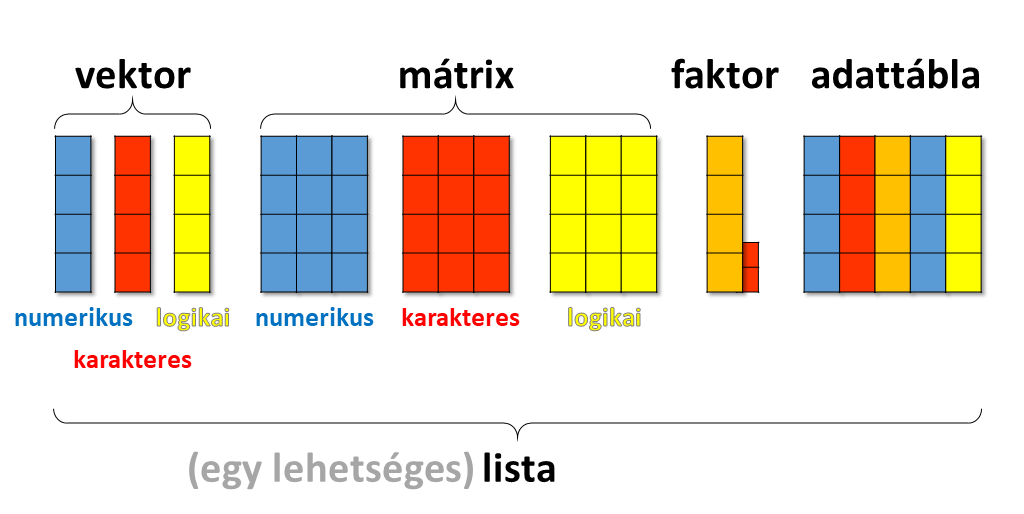
\includegraphics[width=0.85\linewidth]{images/adatszerkezetek_abra} }

}

\caption{Az R legfontosabb adatszerkezetei}\label{fig:adatszerkezetek-1}
\end{figure}

Az \ref{tab:adatszerkezetek}. táblázatban más szempontból mutatjuk be az adatszerkezeteket: példát mutatunk adott típusú (adatszerkezetű) objektumok létrehozására, és közöljük, hogy a \texttt{typeof()} és a \texttt{class()} milyen outputot szolgáltat az így létrehozott objektumok esetében.

\begin{table}

\caption{\label{tab:adatszerkezetek}Adatszerkezetek}
\centering
\resizebox{\linewidth}{!}{
\begin{tabular}[t]{llll}
\toprule
Adatszerkezet & Létrehozó parancs & typeof(x) & class(x)\\
\midrule
\cellcolor{gray!6}{double vektor} & \cellcolor{gray!6}{\ttfamily{c(12, 14)}} & \cellcolor{gray!6}{\ttfamily{double}} & \cellcolor{gray!6}{\ttfamily{numeric}}\\
integer vektor & \ttfamily{c(12L, 14L)} & \ttfamily{integer} & \ttfamily{integer}\\
\cellcolor{gray!6}{karakteres vektor} & \cellcolor{gray!6}{\ttfamily{c('a','az','egy')}} & \cellcolor{gray!6}{\ttfamily{character}} & \cellcolor{gray!6}{\ttfamily{character}}\\
logikai vektor & \ttfamily{c(T, TRUE,FALSE,F)} & \ttfamily{logical} & \ttfamily{logical}\\
\cellcolor{gray!6}{double mátrix} & \cellcolor{gray!6}{\ttfamily{matrix(1.3,nrow=2,ncol=3)}} & \cellcolor{gray!6}{\ttfamily{double}} & \cellcolor{gray!6}{\ttfamily{matrix array}}\\
\addlinespace
integer mátrix & \ttfamily{matrix(1L,nrow=2,ncol=3)} & \ttfamily{integer} & \ttfamily{matrix array}\\
\cellcolor{gray!6}{karakteres mátrix} & \cellcolor{gray!6}{\ttfamily{matrix('az',nrow=2,ncol=3)}} & \cellcolor{gray!6}{\ttfamily{character}} & \cellcolor{gray!6}{\ttfamily{matrix array}}\\
logikai mátrix & \ttfamily{matrix(F,nrow=2,ncol=3)} & \ttfamily{logical} & \ttfamily{matrix array}\\
\cellcolor{gray!6}{faktor} & \cellcolor{gray!6}{\ttfamily{factor(c('D','D','ND'))}} & \cellcolor{gray!6}{\ttfamily{integer}} & \cellcolor{gray!6}{\ttfamily{factor}}\\
lista & \ttfamily{list(A='Pék',B=1:2)} & \ttfamily{list} & \ttfamily{list}\\
\addlinespace
\cellcolor{gray!6}{adattábla} & \cellcolor{gray!6}{\ttfamily{data.frame(id=c('a','b'), pont=c(4,9))}} & \cellcolor{gray!6}{\ttfamily{list}} & \cellcolor{gray!6}{\ttfamily{data.frame}}\\
\bottomrule
\end{tabular}}
\end{table}

A következő alfejezetekben részletesen áttekintjük a \emph{vektor}, a \emph{mátrix}, a \emph{faktor}, a \emph{lista} és az \emph{adattábla} adatszerkezeteket, ugyanis ezek töltik be a legfontosabb szerepet az adatelemzések során. Mindegyik esetben megvizsgáljuk:

\begin{itemize}
\tightlist
\item
  hogyan hozhatjuk létre az adott adatszerkezetű objektumot,
\item
  hogyan tesztelhetjük, hogy az adott típusú objektumról van-e szó,
\item
  hogyan konvertálhatunk más adatszerkezetekből ilyen típusú objektumot,
\item
  milyen műveletekben vehet részt,
\item
  hogyan érhetjük el az objektum részeit, azaz hogyan indexelhetjük az objektumokat.
\end{itemize}

\hypertarget{az-r-nyelv-4-summary}{%
\subsubsection{Összefoglalás}\label{az-r-nyelv-4-summary}}

\begin{rmdsummary}
A különböző típusú konstansokat objektumok létrehozására használhatjuk
fel. A statisztikában egy objektumok értéke több konstans egymásutánja.
A legegyszerűbb adatszerkezet az R-ben a \emph{vektor}, amelyben
tetszőlegesen sok, azonos típusú értéket helyezhetünk el egy dimenzió
mentén. A \emph{faktor} és a \emph{lista} is egydimenziós, míg a
\emph{mátrix} és az \emph{adattábla} kétdimenziós. A \emph{faktor}
integer vektor, amelyben a számoknak címkéket feleltetünk meg. A
\emph{lista} elemi tetszőleges típusúak lehetnek. A \emph{mátrix}
ugyanúgy homogén, minta a \emph{vektor} és a \emph{faktor}. Az
\emph{adattábla} felfogható azonos elemszámú vektorok/faktorok
listájának.
\end{rmdsummary}

\hypertarget{az-r-nyelv-4-exercise}{%
\subsubsection{Feladatok}\label{az-r-nyelv-4-exercise}}

\begin{rmdexercise}
\begin{enumerate}
\def\labelenumi{\arabic{enumi}.}
\tightlist
\item
  Próbáljuk ki az \ref{tab:adatszerkezetek}. táblázatban szereplő példákat. Hozzuk létre a különböző típusú objektumokat és vizsgáljuk meg a \texttt{typeof()} és \texttt{class()} függvényekkel az objektumok típusát.
\end{enumerate}
\end{rmdexercise}

\hypertarget{vektor}{%
\subsection{Vektor}\label{vektor}}

Az R legalapvetőbb adatszerkezete a \emph{vektor}. A vektort egymás melletti (vagy alatti) cellákban tárolt értékek sorozataként képzelhetjük el (\ref{fig:adatszerkezetek-1}. ábra), mely értékek mindegyike azonos típusú. Így azt mondhatjuk, hogy a vektor azonos típusú (egynemű, homogén) adatok egydimenziós együttese. A vektor fontos jellemzője, hogy homogén, tehát a vektort alkotó értékek vagy kizárólag \emph{integer}, vagy kizárólag \emph{double}, vagy kizárólag \emph{karakteres}, vagy kizárólag \emph{logikai} típusúak lehetnek.

\hypertarget{vektor-luxe9trehozuxe1sa}{%
\subsubsection{Vektor létrehozása}\label{vektor-luxe9trehozuxe1sa}}

Vektort legegyszerűbben a \texttt{c()} függvénnyel hozhatunk létre, az argumentumlistában egymás felsoroljuk a vektort alkotó értékeket. \emph{Double} vektort hozhatunk létre például, ha a paraméterben numerikus konstansokat sorolunk fel:

\begin{Shaded}
\begin{Highlighting}[]
\NormalTok{v.d }\OtherTok{\textless{}{-}} \FunctionTok{c}\NormalTok{(}\DecValTok{2}\NormalTok{, }\DecValTok{4}\NormalTok{, }\DecValTok{6}\NormalTok{, }\DecValTok{8}\NormalTok{); v.d  }\CommentTok{\# numerikus (double) vektor létrehozása}
\CommentTok{\#\textgreater{} [1] 2 4 6 8}
\end{Highlighting}
\end{Shaded}

A \texttt{v.d} objektum egy 4 elemű \emph{double} vektor. Az első eleme a 2, a második eleme a 4, a harmadik a 6 és a negyedik egyben utolsó eleme a 8. A vektor elemei szóközökkel elválasztva jelennek meg a konzolban.

Karakteres vektort hasonlóan hozhatunk létre, a \texttt{v.k} vektor 3 elemű lesz.

\begin{Shaded}
\begin{Highlighting}[]
\NormalTok{v.k }\OtherTok{\textless{}{-}} \FunctionTok{c}\NormalTok{(}\StringTok{"erős"}\NormalTok{, }\StringTok{\textquotesingle{}közepes\textquotesingle{}}\NormalTok{, }\StringTok{"gyenge"}\NormalTok{); v.k }\CommentTok{\# karakteres vektor létrehozása}
\CommentTok{\#\textgreater{} [1] "erős"    "közepes" "gyenge"}
\end{Highlighting}
\end{Shaded}

Egy logikai vektor csak logikai konstansokat tartalmazhat (\texttt{TRUE} vagy \texttt{FALSE}, illetve a \texttt{T} és \texttt{F} rövidebb változatot is használhatjuk):

\begin{Shaded}
\begin{Highlighting}[]
\NormalTok{v.l }\OtherTok{\textless{}{-}} \FunctionTok{c}\NormalTok{(}\ConstantTok{TRUE}\NormalTok{, }\ConstantTok{FALSE}\NormalTok{, T); v.l  }\CommentTok{\# logikai vektor létrehozása}
\CommentTok{\#\textgreater{} [1]  TRUE FALSE  TRUE}
\end{Highlighting}
\end{Shaded}

A \texttt{v.d}, \texttt{v.k} és \texttt{v.l} objektum egy-egy példa az R különböző típusú vektoraira. Az objektumok fontos jellemzője az objektum hossza, ami vektorok esetén a vektort alkotó elemek számát jelenti. Ezt a \texttt{length()} függvénnyel kérdezhetjük le.

\begin{Shaded}
\begin{Highlighting}[]
\FunctionTok{length}\NormalTok{(v.d); }\FunctionTok{length}\NormalTok{(v.k); }\FunctionTok{length}\NormalTok{(v.l)  }\CommentTok{\# vektor hossza}
\CommentTok{\#\textgreater{} [1] 4}
\CommentTok{\#\textgreater{} [1] 3}
\CommentTok{\#\textgreater{} [1] 3}
\end{Highlighting}
\end{Shaded}

A vektor hosszát létrehozása után is módosíthatjuk, szintén a \texttt{length()} függvényt használjuk, de az értékadás bal oldalán.

\begin{Shaded}
\begin{Highlighting}[]
\FunctionTok{length}\NormalTok{(v.l) }\OtherTok{\textless{}{-}} \DecValTok{5}  \CommentTok{\# vektor hosszának módosítása}
\end{Highlighting}
\end{Shaded}

A \texttt{v.l} logikai vektor most már 5 elemű lesz:

\begin{Shaded}
\begin{Highlighting}[]
\NormalTok{v.l}
\CommentTok{\#\textgreater{} [1]  TRUE FALSE  TRUE    NA    NA}
\end{Highlighting}
\end{Shaded}

Mivel nem adtuk meg a 4. és 5. elemét, így az \texttt{NA} lesz, ami a \emph{hiányzó érték} jele az R-ben. Az \texttt{NA} minden vektornak eleme lehet, a vektor típusától függetlenül.

\begin{Shaded}
\begin{Highlighting}[]
\NormalTok{v.i }\OtherTok{\textless{}{-}} \FunctionTok{c}\NormalTok{(12L, }\ConstantTok{NA}\NormalTok{, 15L)  }\CommentTok{\# 3 elemű integer vektor; a 2. eleme nem ismert}
\end{Highlighting}
\end{Shaded}

Térjünk vissza a vektorok létrehozásához. A \texttt{c()} függvény paraméterébe természetesen konstansok helyett tetszőleges kifejezéseket is írhatunk:

\begin{Shaded}
\begin{Highlighting}[]
\NormalTok{szamok }\OtherTok{\textless{}{-}} \FunctionTok{c}\NormalTok{(}\DecValTok{1}\NormalTok{, (}\DecValTok{2}\SpecialCharTok{+}\DecValTok{3}\NormalTok{)}\SpecialCharTok{*}\DecValTok{4}\NormalTok{, }\DecValTok{1}\SpecialCharTok{/}\DecValTok{4}\NormalTok{, .}\DecValTok{5}\SpecialCharTok{\^{}}\DecValTok{3}\NormalTok{);        szamok}
\CommentTok{\#\textgreater{} [1]  1.000 20.000  0.250  0.125}
\NormalTok{nevek  }\OtherTok{\textless{}{-}} \FunctionTok{c}\NormalTok{(}\StringTok{"Péter"}\NormalTok{, }\FunctionTok{paste0}\NormalTok{(}\StringTok{\textquotesingle{}Zso\textquotesingle{}}\NormalTok{, }\StringTok{"lt"}\NormalTok{)); nevek}
\CommentTok{\#\textgreater{} [1] "Péter" "Zsolt"}
\NormalTok{iteletek }\OtherTok{\textless{}{-}} \FunctionTok{c}\NormalTok{(T, }\DecValTok{1}\SpecialCharTok{\textless{}}\DecValTok{2}\NormalTok{, }\DecValTok{2}\SpecialCharTok{==}\DecValTok{3}\NormalTok{);               iteletek}
\CommentTok{\#\textgreater{} [1]  TRUE  TRUE FALSE}
\end{Highlighting}
\end{Shaded}

A vektorok esetében a homogenitás központi szerepet játszik. Az R abban az esetben sem fog különböző típusú elemekből vektort létrehozni, ha ezeket egyetlen \texttt{c()} függvényhívásban szerepeltetjük. Ekkor automatikus típuskonverzió történik. Nézzük ezeknek az eseteit:

\begin{Shaded}
\begin{Highlighting}[]
\NormalTok{eset}\FloatTok{.1} \OtherTok{\textless{}{-}} \FunctionTok{c}\NormalTok{(}\DecValTok{2}\NormalTok{,}\DecValTok{4}\NormalTok{,}\StringTok{"6"}\NormalTok{,}\DecValTok{8}\NormalTok{);    eset}\FloatTok{.1}
\CommentTok{\#\textgreater{} [1] "2" "4" "6" "8"}
\NormalTok{eset}\FloatTok{.2} \OtherTok{\textless{}{-}} \FunctionTok{c}\NormalTok{(T, }\ConstantTok{FALSE}\NormalTok{,}\StringTok{"6"}\NormalTok{); eset}\FloatTok{.2}
\CommentTok{\#\textgreater{} [1] "TRUE"  "FALSE" "6"}
\NormalTok{eset}\FloatTok{.3} \OtherTok{\textless{}{-}} \FunctionTok{c}\NormalTok{(T, }\ConstantTok{FALSE}\NormalTok{, }\DecValTok{3}\NormalTok{);  eset}\FloatTok{.3}
\CommentTok{\#\textgreater{} [1] 1 0 3}
\end{Highlighting}
\end{Shaded}

Amennyiben karakteres konstans szerepel az elemek között, a vektor karakteres típusú lesz. Ha numerikus és logikai értéket sorolunk fel, akkor a vektor numerikus lesz, azzal a kiegészítéssel, hogy a \texttt{TRUE} logikai érték 1-re, a \texttt{FALSE} pedig 0-ra konvertálódik.

További lehetőség a \texttt{c()} függvény használata során, hogy a paraméterben vektort is szerepeltethetünk. Ekkor ezek az elemek is szerepelni fognak az eredményvektorban:

\begin{Shaded}
\begin{Highlighting}[]
\NormalTok{regi.v}\FloatTok{.1} \OtherTok{\textless{}{-}} \FunctionTok{c}\NormalTok{(}\DecValTok{1}\NormalTok{, }\DecValTok{2}\NormalTok{, }\DecValTok{3}\NormalTok{)}
\NormalTok{regi.v}\FloatTok{.2} \OtherTok{\textless{}{-}} \FunctionTok{c}\NormalTok{(}\DecValTok{7}\NormalTok{, }\DecValTok{8}\NormalTok{, }\DecValTok{9}\NormalTok{)}
\NormalTok{uj.v }\OtherTok{\textless{}{-}} \FunctionTok{c}\NormalTok{(}\DecValTok{0}\NormalTok{, regi.v}\FloatTok{.1}\NormalTok{, }\DecValTok{4}\NormalTok{, }\DecValTok{5}\NormalTok{, }\DecValTok{6}\NormalTok{, regi.v}\FloatTok{.2}\NormalTok{, }\DecValTok{10}\NormalTok{, }\FunctionTok{c}\NormalTok{(}\DecValTok{11}\NormalTok{, }\DecValTok{12}\NormalTok{)); uj.v}
\CommentTok{\#\textgreater{}  [1]  0  1  2  3  4  5  6  7  8  9 10 11 12}
\end{Highlighting}
\end{Shaded}

A fenti példában létrehozott \texttt{uj.v} 13 elemű numerikus vektor összerakásához felhasználtunk két 3 elemű vektort és egy kételemű vektort is.

Vektorok létrehozása során még egy érdekes lehetőségről érdemes szót ejteni. A \texttt{c()} függvényben a vektor egyes elemeit elnevezhetjük, és ezek a nevek az outputban is meg fognak jelenni. Az elemek elnevezéséhez írjunk egy nevet és egy egyenlőségjelet az argumentumként használt elem elé. Ha a név nem egyetlen szó (vagyis tartalmaz szóközt), akkor a karakterkonstansok megadásánál látott három módszer valamelyikét használhatjuk (tehát a dupla és szimpla idézőjeleket és az \texttt{r"()"} konstrukciót), vagy a backtick (`) szimbólumot. Ezzel a módszerrel például a naponta tanulással töltött időnket úgy rögzíthetjük, hogy az output ``beszédesebb'' lesz, több információt tartalmaz.

\begin{Shaded}
\begin{Highlighting}[]
\NormalTok{tan.ido }\OtherTok{\textless{}{-}} \FunctionTok{c}\NormalTok{(Hétfő}\OtherTok{=}\DecValTok{35}\NormalTok{, }\AttributeTok{Kedd=}\DecValTok{95}\NormalTok{); tan.ido}
\CommentTok{\#\textgreater{} Hétfő  Kedd }
\CommentTok{\#\textgreater{}    35    95}
\NormalTok{tan.ido }\OtherTok{\textless{}{-}} \FunctionTok{c}\NormalTok{(Hétfő}\OtherTok{=}\DecValTok{35}\NormalTok{, }\StringTok{"Kedd délelőtt"}\OtherTok{=}\DecValTok{50}\NormalTok{, }\StringTok{\textasciigrave{}}\AttributeTok{Kedd délután}\StringTok{\textasciigrave{}}\OtherTok{=}\DecValTok{45}\NormalTok{); tan.ido}
\CommentTok{\#\textgreater{}         Hétfő Kedd délelőtt  Kedd délután }
\CommentTok{\#\textgreater{}            35            50            45}
\end{Highlighting}
\end{Shaded}

A vektorelemek nevei lekérdezhetők a \texttt{names()} függvénnyel. Amennyiben az értékadás bal oldalán szerepeltetjük, a vektor elemneveit tudjuk módosítani.

\begin{Shaded}
\begin{Highlighting}[]
\FunctionTok{names}\NormalTok{(tan.ido)                         }\CommentTok{\# elemnevek lekérdezése}
\CommentTok{\#\textgreater{} [1] "Hétfő"         "Kedd délelőtt" "Kedd délután"}
\FunctionTok{names}\NormalTok{(tan.ido) }\OtherTok{\textless{}{-}} \FunctionTok{c}\NormalTok{(}\StringTok{"H"}\NormalTok{, }\StringTok{"K.1"}\NormalTok{, }\StringTok{"K.2"}\NormalTok{) }\CommentTok{\# elemnevek módosítása}
\NormalTok{tan.ido}
\CommentTok{\#\textgreater{}   H K.1 K.2 }
\CommentTok{\#\textgreater{}  35  50  45}
\end{Highlighting}
\end{Shaded}

\hypertarget{szabalyosvektorokalfejezet}{%
\subsubsection{Szabályos vektorok létrehozása}\label{szabalyosvektorokalfejezet}}

Ha egy vektor elemei szabályos rendben követik egymást, akkor szabályos vektorokról beszélünk. Ilyen lehet például a következő három numerikus vektor és két karakteres vektor.

\begin{Shaded}
\begin{Highlighting}[]
\FunctionTok{c}\NormalTok{(}\DecValTok{1}\NormalTok{, }\DecValTok{2}\NormalTok{, }\DecValTok{3}\NormalTok{, }\DecValTok{4}\NormalTok{, }\DecValTok{5}\NormalTok{); }\FunctionTok{c}\NormalTok{(}\DecValTok{1}\NormalTok{, }\DecValTok{3}\NormalTok{, }\DecValTok{5}\NormalTok{, }\DecValTok{7}\NormalTok{); }\FunctionTok{c}\NormalTok{(}\DecValTok{1}\NormalTok{, }\DecValTok{1}\NormalTok{, }\DecValTok{1}\NormalTok{, }\DecValTok{2}\NormalTok{, }\DecValTok{2}\NormalTok{, }\DecValTok{2}\NormalTok{)}
\FunctionTok{c}\NormalTok{(}\StringTok{"férfi"}\NormalTok{, }\StringTok{"nő"}\NormalTok{, }\StringTok{"férfi"}\NormalTok{, }\StringTok{"nő"}\NormalTok{); }\FunctionTok{c}\NormalTok{(}\StringTok{"f.1"}\NormalTok{, }\StringTok{"f.2"}\NormalTok{, }\StringTok{"f.3"}\NormalTok{)}
\end{Highlighting}
\end{Shaded}

Szabályos numerikus vektorokat hozhatunk létre a kettőspont (\texttt{:}) operátorral vagy a \texttt{seq()} függvénnyel. Az így létrehozott vektorok ugyanis valamilyen számtani sorozat egymást követő elemei, vagyis az egymás mellett lévő elemek különbsége (a lépésköz) állandó.

\hypertarget{a-kettux151spont-operuxe1tor.}{%
\paragraph{A kettőspont operátor.}\label{a-kettux151spont-operuxe1tor.}}

A legegyszerűbb vektorlétrehozási mód a kettőspont (\texttt{:}) operátor, ahol az egymást követő elemek távolsága 1 vagy -1. Általános alakja: \texttt{start:stop}.

\begin{Shaded}
\begin{Highlighting}[]
\DecValTok{1}\SpecialCharTok{:}\DecValTok{10}    \CommentTok{\# a lépésköz +1, növekvő sorozat}
\CommentTok{\#\textgreater{}  [1]  1  2  3  4  5  6  7  8  9 10}
\DecValTok{10}\SpecialCharTok{:}\DecValTok{1}    \CommentTok{\# a lépésköz {-}1, csökkenő sorozat}
\CommentTok{\#\textgreater{}  [1] 10  9  8  7  6  5  4  3  2  1}
\SpecialCharTok{{-}}\FloatTok{1.5}\SpecialCharTok{:}\DecValTok{5}  \CommentTok{\# a lépésköz +1, növekvő sorozat}
\CommentTok{\#\textgreater{} [1] {-}1.5 {-}0.5  0.5  1.5  2.5  3.5  4.5}
\FloatTok{10.5}\SpecialCharTok{:}\DecValTok{3}  \CommentTok{\# a lépésköz {-}1, csökkenő sorozat}
\CommentTok{\#\textgreater{} [1] 10.5  9.5  8.5  7.5  6.5  5.5  4.5  3.5}
\end{Highlighting}
\end{Shaded}

Látható, hogy az így létrehozott vektorok lehetnek csökkenő vagy növekvő rendezettségűek, valamint tört értékeket is használhatunk operandusként. A sorozat nem feltétlenül a kettőspont utáni értékig tart, mindössze annyi igaz, hogy a sorozat vége a \texttt{stop} értéknél mindig kisebb egyenlő (vagy nagyobb egyenlő, csökkenő sorozat esetén).

Hosszabb numerikus vektorokat is könnyűszerrel létrehozhatunk. A \texttt{101:140} parancs hatására 40 elemet hozunk létre. Hosszabb vektorok outputjában könnyebben el tudunk igazodni a sorok elején lévő \texttt{{[}x{]}} konstrukció segítségével: minden sorban a sor első eleme a vektor \texttt{x.} eleme. A lenti outputban szereplő \texttt{{[}17{]}} például azt mutatja, hogy a sor elején lévő 117 a 40 elemű vektor 17. eleme.

\begin{Shaded}
\begin{Highlighting}[]
\DecValTok{101}\SpecialCharTok{:}\DecValTok{140}  \CommentTok{\# a lépésköz +1, növekvő sorozat}
\CommentTok{\#\textgreater{}  [1] 101 102 103 104 105 106 107 108 109 110 111 112 113 114 115 116}
\CommentTok{\#\textgreater{} [17] 117 118 119 120 121 122 123 124 125 126 127 128 129 130 131 132}
\CommentTok{\#\textgreater{} [33] 133 134 135 136 137 138 139 140}
\end{Highlighting}
\end{Shaded}

\hypertarget{a-seq-fuxfcggvuxe9ny}{%
\paragraph{\texorpdfstring{A \texttt{seq()} függvény}{A seq() függvény}}\label{a-seq-fuxfcggvuxe9ny}}

A \texttt{seq()} függvény nagyobb szabadságot ad a numerikus sorozatok generálására. Legegyszerűbb használata esetén a kettőspont (\texttt{:}) operátort kapjuk vissza:

\begin{Shaded}
\begin{Highlighting}[]
\FunctionTok{seq}\NormalTok{(}\DecValTok{1}\NormalTok{, }\DecValTok{10}\NormalTok{) }\CommentTok{\# a lépésköz +1, növekvő sorozat}
\CommentTok{\#\textgreater{}  [1]  1  2  3  4  5  6  7  8  9 10}
\end{Highlighting}
\end{Shaded}

A \texttt{seq()} függvény használatához négy argumentum nevét és jelentését kell megtanulnunk: a \texttt{from=} a sorozat első elemét határozza meg, a \texttt{to=} az utolsó elemet, a \texttt{by=} a lépésközt és a \texttt{length.out=} a létrehozandó vektor elemeinek a számát. A négy paraméterből három megadása már egyértelműen azonosítja a kívánt vektort:

\begin{Shaded}
\begin{Highlighting}[]
\FunctionTok{seq}\NormalTok{(}\AttributeTok{from=}\DecValTok{1}\NormalTok{, }\AttributeTok{to=}\DecValTok{10}\NormalTok{, }\AttributeTok{by=}\DecValTok{2}\NormalTok{)           }\CommentTok{\# a lépésköz +2, növekvő sorozat}
\CommentTok{\#\textgreater{} [1] 1 3 5 7 9}
\FunctionTok{seq}\NormalTok{(}\AttributeTok{from=}\DecValTok{1}\NormalTok{, }\AttributeTok{to=}\DecValTok{10}\NormalTok{, }\AttributeTok{length.out=}\DecValTok{5}\NormalTok{)   }\CommentTok{\# a lépésköz +2.25, növekvő sorozat}
\CommentTok{\#\textgreater{} [1]  1.00  3.25  5.50  7.75 10.00}
\FunctionTok{seq}\NormalTok{(}\AttributeTok{to=}\DecValTok{10}\NormalTok{, }\AttributeTok{by=}\SpecialCharTok{{-}}\FloatTok{1.3}\NormalTok{, }\AttributeTok{length.out=}\DecValTok{5}\NormalTok{)  }\CommentTok{\# a lépésköz {-}1.3, csökkenő sorozat}
\CommentTok{\#\textgreater{} [1] 15.2 13.9 12.6 11.3 10.0}
\FunctionTok{seq}\NormalTok{(}\AttributeTok{from=}\DecValTok{1}\NormalTok{, }\AttributeTok{by=}\FloatTok{1.3}\NormalTok{, }\AttributeTok{length.out=}\DecValTok{5}\NormalTok{)  }\CommentTok{\# a lépésköz +1.3, növekvő sorozat}
\CommentTok{\#\textgreater{} [1] 1.0 2.3 3.6 4.9 6.2}
\end{Highlighting}
\end{Shaded}

A \texttt{seq\_along()} függvénnyel szintén tudunk 1-től induló, +1-es lépésközű sorozatot alkotni, amelynek utolsó értéke, a paraméterben megadott vektor elemszáma.

\begin{Shaded}
\begin{Highlighting}[]
\NormalTok{x }\OtherTok{\textless{}{-}} \FunctionTok{c}\NormalTok{(}\StringTok{"Hétfő"}\NormalTok{, }\StringTok{"Kedd"}\NormalTok{, }\StringTok{"Szerda"}\NormalTok{); y }\OtherTok{\textless{}{-}} \DecValTok{11}\SpecialCharTok{:}\DecValTok{20}
\FunctionTok{seq\_along}\NormalTok{(x) }\CommentTok{\# numerikus vektor 1{-}től, +1{-}es lépésközzel, 3 elemű}
\CommentTok{\#\textgreater{} [1] 1 2 3}
\FunctionTok{seq\_along}\NormalTok{(y) }\CommentTok{\# numerikus vektor 1{-}től, +1{-}es lépésközzel, 10 elemű}
\CommentTok{\#\textgreater{}  [1]  1  2  3  4  5  6  7  8  9 10}
\end{Highlighting}
\end{Shaded}

\hypertarget{a-rep-fuxfcggvuxe9ny}{%
\paragraph{\texorpdfstring{A \texttt{rep()} függvény}{A rep() függvény}}\label{a-rep-fuxfcggvuxe9ny}}

Tetszőleges típusú vektor létrehozására használhatjuk a \texttt{rep()} függvényt, amely egy létező vektor értékeit ismétli meg. A \texttt{rep()} első paramétere az ismétlendő vektor, a \texttt{times=} pedig az ismétlések számát adja meg.

\begin{Shaded}
\begin{Highlighting}[]
\FunctionTok{rep}\NormalTok{(}\DecValTok{2}\NormalTok{, }\AttributeTok{times=}\DecValTok{3}\NormalTok{)            }\CommentTok{\# számot ismétlünk 3{-}szor}
\CommentTok{\#\textgreater{} [1] 2 2 2}
\FunctionTok{rep}\NormalTok{(}\FunctionTok{c}\NormalTok{(}\DecValTok{2}\NormalTok{, }\DecValTok{0}\NormalTok{, }\SpecialCharTok{{-}}\DecValTok{2}\NormalTok{), }\AttributeTok{times=}\DecValTok{3}\NormalTok{)  }\CommentTok{\# numerikus vektort ismétlünk 3{-}szor}
\CommentTok{\#\textgreater{} [1]  2  0 {-}2  2  0 {-}2  2  0 {-}2}
\FunctionTok{rep}\NormalTok{(}\StringTok{"nap"}\NormalTok{, }\AttributeTok{times=}\DecValTok{3}\NormalTok{)        }\CommentTok{\# sztringet ismétlünk 3{-}szor}
\CommentTok{\#\textgreater{} [1] "nap" "nap" "nap"}
\FunctionTok{rep}\NormalTok{(}\FunctionTok{c}\NormalTok{(F, T, T), }\AttributeTok{times=}\DecValTok{3}\NormalTok{)   }\CommentTok{\# logikai vektort ismétlünk 3{-}szor}
\CommentTok{\#\textgreater{} [1] FALSE  TRUE  TRUE FALSE  TRUE  TRUE FALSE  TRUE  TRUE}
\end{Highlighting}
\end{Shaded}

A fenti példában mindenhol háromszor ismételtük meg az első paramétert, méghozzá úgy, hogy az R egymás után sorolta fel őket.

Egy vektor ismétlésének van egy másik esete is, amikor az elemeit sorban egyenként véve végezzük el az ismétlést (helyben ismétlés). Ekkor nem a \texttt{times=} paramétert, hanem az \texttt{each=} argumentumot kell használnunk a függvény hívásánál.

\begin{Shaded}
\begin{Highlighting}[]
\FunctionTok{rep}\NormalTok{(}\DecValTok{2}\NormalTok{, }\AttributeTok{each=}\DecValTok{3}\NormalTok{)            }\CommentTok{\# számot ismétlünk 3{-}szor}
\CommentTok{\#\textgreater{} [1] 2 2 2}
\FunctionTok{rep}\NormalTok{(}\FunctionTok{c}\NormalTok{(}\DecValTok{2}\NormalTok{, }\DecValTok{0}\NormalTok{, }\SpecialCharTok{{-}}\DecValTok{2}\NormalTok{), }\AttributeTok{each=}\DecValTok{3}\NormalTok{)  }\CommentTok{\# numerikus vektort elemeit ismételjük 3{-}szor}
\CommentTok{\#\textgreater{} [1]  2  2  2  0  0  0 {-}2 {-}2 {-}2}
\FunctionTok{rep}\NormalTok{(}\StringTok{"nap"}\NormalTok{, }\AttributeTok{each=}\DecValTok{3}\NormalTok{)        }\CommentTok{\# sztringet ismétlünk 3{-}szor}
\CommentTok{\#\textgreater{} [1] "nap" "nap" "nap"}
\FunctionTok{rep}\NormalTok{(}\FunctionTok{c}\NormalTok{(F,T,T), }\AttributeTok{each=}\DecValTok{3}\NormalTok{)     }\CommentTok{\# logikai vektor elemeit ismételjük 3{-}szor}
\CommentTok{\#\textgreater{} [1] FALSE FALSE FALSE  TRUE  TRUE  TRUE  TRUE  TRUE  TRUE}
\end{Highlighting}
\end{Shaded}

Látjuk, hogy egyelemű vektorok ismétlése esetén nincs különbség a \texttt{times=} és az \texttt{each=} paraméterek használata között.

Utolsó esetként elemenként szeretnénk ismételni, de eltérő ismétlésszámmal. Ekkor a \texttt{times=} paraméterben a bemenő vektor elemszámával azonos hosszú vektort kell megadni. Ez a vektor tartalmazza az elemek ismétlés számát.

\begin{Shaded}
\begin{Highlighting}[]
\FunctionTok{rep}\NormalTok{(}\FunctionTok{c}\NormalTok{(}\DecValTok{2}\NormalTok{, }\DecValTok{3}\NormalTok{, }\DecValTok{4}\NormalTok{), }\AttributeTok{times=}\FunctionTok{c}\NormalTok{(}\DecValTok{1}\NormalTok{, }\DecValTok{2}\NormalTok{, }\DecValTok{3}\NormalTok{))    }\CommentTok{\# numerikus vektort elemeit ismételjük}
\CommentTok{\#\textgreater{} [1] 2 3 3 4 4 4}
\FunctionTok{rep}\NormalTok{(}\FunctionTok{c}\NormalTok{(}\StringTok{"nap"}\NormalTok{, }\StringTok{"part"}\NormalTok{), }\AttributeTok{times=}\FunctionTok{c}\NormalTok{(}\DecValTok{2}\NormalTok{, }\DecValTok{3}\NormalTok{)) }\CommentTok{\# karakteres vektort elemeit ismételjük}
\CommentTok{\#\textgreater{} [1] "nap"  "nap"  "part" "part" "part"}
\FunctionTok{rep}\NormalTok{(}\FunctionTok{c}\NormalTok{(T, F, T), }\AttributeTok{times=}\FunctionTok{c}\NormalTok{(}\DecValTok{2}\NormalTok{, }\DecValTok{3}\NormalTok{, }\DecValTok{4}\NormalTok{))    }\CommentTok{\# logikai vektort elemeit ismételjük}
\CommentTok{\#\textgreater{} [1]  TRUE  TRUE FALSE FALSE FALSE  TRUE  TRUE  TRUE  TRUE}
\end{Highlighting}
\end{Shaded}

Végezetül bemutatjuk, hogy az \texttt{each=} és az egyelemű értékkel rendelkező \texttt{times=} egyszerre is alkalmazható. Ekkor először a helyben ismétlés (\texttt{each=}), majd az így kapott vektor teljes ismétlése következik (\texttt{times=}).

\begin{Shaded}
\begin{Highlighting}[]
\FunctionTok{rep}\NormalTok{(}\DecValTok{1}\SpecialCharTok{:}\DecValTok{5}\NormalTok{, }\AttributeTok{each=}\DecValTok{2}\NormalTok{, }\AttributeTok{times=}\DecValTok{3}\NormalTok{) }\CommentTok{\# kombinált ismétlés}
\CommentTok{\#\textgreater{}  [1] 1 1 2 2 3 3 4 4 5 5 1 1 2 2 3 3 4 4 5 5 1 1 2 2 3 3 4 4 5 5}
\end{Highlighting}
\end{Shaded}

\hypertarget{a-paste-fuxfcggvuxe9ny}{%
\paragraph{\texorpdfstring{A \texttt{paste()} függvény}{A paste() függvény}}\label{a-paste-fuxfcggvuxe9ny}}

Szabályos karakteres vektor létrehozására használhatjuk a \texttt{paste()} függvényt. Egy előtaghoz (például \texttt{f}) hozzáfűzhetünk 10 különböző számot, amely így egy 10 elemű karakteres vektort eredményez.

\begin{Shaded}
\begin{Highlighting}[]
\FunctionTok{paste}\NormalTok{(}\StringTok{"f"}\NormalTok{, }\DecValTok{1}\SpecialCharTok{:}\DecValTok{10}\NormalTok{) }\CommentTok{\# 10 elemű sztring vektor}
\CommentTok{\#\textgreater{}  [1] "f 1"  "f 2"  "f 3"  "f 4"  "f 5"  "f 6"  "f 7"  "f 8"  "f 9"  "f 10"}
\end{Highlighting}
\end{Shaded}

Láthatjuk, hogy az \texttt{f} karakter és a számok közé egy szóköz került, de ezt a \texttt{sep=} argumentummal megváltoztathatjuk:

\begin{Shaded}
\begin{Highlighting}[]
\FunctionTok{paste}\NormalTok{(}\StringTok{"f"}\NormalTok{, }\DecValTok{1}\SpecialCharTok{:}\DecValTok{10}\NormalTok{, }\AttributeTok{sep=}\StringTok{"{-}"}\NormalTok{) }\CommentTok{\# gondolatjel az elválasztó}
\CommentTok{\#\textgreater{}  [1] "f{-}1"  "f{-}2"  "f{-}3"  "f{-}4"  "f{-}5"  "f{-}6"  "f{-}7"  "f{-}8"  "f{-}9"  "f{-}10"}
\FunctionTok{paste}\NormalTok{(}\StringTok{"f"}\NormalTok{, }\DecValTok{1}\SpecialCharTok{:}\DecValTok{10}\NormalTok{, }\AttributeTok{sep=}\StringTok{""}\NormalTok{)  }\CommentTok{\# nincs elválasztó}
\CommentTok{\#\textgreater{}  [1] "f1"  "f2"  "f3"  "f4"  "f5"  "f6"  "f7"  "f8"  "f9"  "f10"}
\end{Highlighting}
\end{Shaded}

A \texttt{collapse=} argumentum használatával, akár egyetlen karakteres értékbe is összeolvaszthatjuk a fenti elemeket. Az argumentumban az összevonásnál használt elválasztó karaktert adjuk meg.

\begin{Shaded}
\begin{Highlighting}[]
\FunctionTok{paste}\NormalTok{(}\StringTok{"f"}\NormalTok{, }\DecValTok{1}\SpecialCharTok{:}\DecValTok{10}\NormalTok{, }\AttributeTok{sep=}\StringTok{"{-}"}\NormalTok{, }\AttributeTok{collapse=}\StringTok{"\_"}\NormalTok{) }\CommentTok{\# gondolatjel az elválasztó, egy sztring}
\CommentTok{\#\textgreater{} [1] "f{-}1\_f{-}2\_f{-}3\_f{-}4\_f{-}5\_f{-}6\_f{-}7\_f{-}8\_f{-}9\_f{-}10"}
\end{Highlighting}
\end{Shaded}

Az eddigiek összefoglalásaként nézzünk példát különböző típusú és elemhosszú vektorok létrehozására.

\begin{Shaded}
\begin{Highlighting}[]
\NormalTok{y }\OtherTok{\textless{}{-}}\NormalTok{ 12L                        }\CommentTok{\# 1 elemű integer vektor}
\NormalTok{y }\OtherTok{\textless{}{-}} \DecValTok{12}                         \CommentTok{\# 1 elemű double vektor}
\NormalTok{y }\OtherTok{\textless{}{-}} \StringTok{"Bízz magadban!"}           \CommentTok{\# 1 elemű karakteres vektor}
\NormalTok{y }\OtherTok{\textless{}{-}} \ConstantTok{TRUE}                       \CommentTok{\# 1 elemű logikai vektor}
\NormalTok{y }\OtherTok{\textless{}{-}} \FunctionTok{c}\NormalTok{(}\FloatTok{23.8}\NormalTok{, }\SpecialCharTok{{-}}\DecValTok{5}\NormalTok{)                }\CommentTok{\# 2 elemű double vektor}
\NormalTok{y }\OtherTok{\textless{}{-}} \FunctionTok{c}\NormalTok{(}\StringTok{"H"}\NormalTok{, }\StringTok{"K"}\NormalTok{)                }\CommentTok{\# 2 elemű karakteres vektor}
\NormalTok{y }\OtherTok{\textless{}{-}} \FunctionTok{c}\NormalTok{(T, }\ConstantTok{FALSE}\NormalTok{)                }\CommentTok{\# 2 elemű logikai vektor}
\NormalTok{y }\OtherTok{\textless{}{-}} \FunctionTok{c}\NormalTok{(}\DecValTok{1}\NormalTok{, }\DecValTok{2}\NormalTok{, }\DecValTok{3}\NormalTok{, }\DecValTok{4}\NormalTok{, }\DecValTok{5}\NormalTok{)           }\CommentTok{\# 5 elemű double vektor}
\NormalTok{y }\OtherTok{\textless{}{-}} \DecValTok{1}\SpecialCharTok{:}\DecValTok{5}                        \CommentTok{\# 5 elemű integer vektor}
\NormalTok{y }\OtherTok{\textless{}{-}} \FunctionTok{seq}\NormalTok{(}\AttributeTok{from=}\DecValTok{9}\NormalTok{, }\AttributeTok{to=}\DecValTok{100}\NormalTok{, }\AttributeTok{by=}\DecValTok{2}\NormalTok{)  }\CommentTok{\# 46 elemű double vektor}
\NormalTok{y }\OtherTok{\textless{}{-}} \FunctionTok{rep}\NormalTok{(}\FunctionTok{c}\NormalTok{(}\StringTok{"H"}\NormalTok{, }\StringTok{"K"}\NormalTok{), }\AttributeTok{times=}\DecValTok{10}\NormalTok{) }\CommentTok{\# 20 elemű karakteres vektor}
\NormalTok{z }\OtherTok{\textless{}{-}} \FunctionTok{seq\_along}\NormalTok{(y)               }\CommentTok{\# 20 elemű integer vektor}
\NormalTok{y }\OtherTok{\textless{}{-}} \FunctionTok{paste}\NormalTok{(}\StringTok{"év"}\NormalTok{, }\DecValTok{2001}\SpecialCharTok{:}\DecValTok{2020}\NormalTok{)     }\CommentTok{\# 20 elemű karakteres vektor}
\end{Highlighting}
\end{Shaded}

\hypertarget{a-vektoraritmetika-szabuxe1lyai}{%
\subsubsection{A vektoraritmetika szabályai}\label{a-vektoraritmetika-szabuxe1lyai}}

Amint az előzőekben láttuk, az R rendszer legalapvetőbb adattárolási szerkezete a vektor. Az R egyik legnagyszerűbb tulajdonsága pedig az, ahogyan a vektorokkal műveleteket végezhetünk. Korábban már láttuk, hogyan tudunk összeadni két számot az R-ben. Próbáljunk meg összeadni két 2 elemű vektort:

\begin{Shaded}
\begin{Highlighting}[]
\FunctionTok{c}\NormalTok{(}\DecValTok{1}\NormalTok{, }\DecValTok{2}\NormalTok{) }\SpecialCharTok{+} \FunctionTok{c}\NormalTok{(}\DecValTok{3}\NormalTok{, }\DecValTok{4}\NormalTok{) }\CommentTok{\# két vektor összeadása}
\CommentTok{\#\textgreater{} [1] 4 6}
\end{Highlighting}
\end{Shaded}

A két fenti vektort a parancssorban hoztuk létre a \texttt{c()} függvénnyel. Az összeadás eredménye egy 2 elemű vektor. Az eredményvektor az \texttt{1+3} és a \texttt{2+4} műveletek alapján jött létre, vagyis az összeadás operandusaiban szereplő vektor azonos sorszámú elemeire hajtotta végre a kijelölt műveletet az R.

Két vektor összeadásánál természetesen használhatunk objektumneveket is:

\begin{Shaded}
\begin{Highlighting}[]
\NormalTok{x }\OtherTok{\textless{}{-}} \FunctionTok{c}\NormalTok{(}\DecValTok{1}\NormalTok{, }\DecValTok{2}\NormalTok{, }\DecValTok{3}\NormalTok{); y }\OtherTok{\textless{}{-}} \FunctionTok{c}\NormalTok{(}\DecValTok{2}\NormalTok{, }\DecValTok{3}\NormalTok{, }\DecValTok{4}\NormalTok{)}
\NormalTok{x }\SpecialCharTok{+}\NormalTok{ y }\CommentTok{\# két vektor összeadása}
\CommentTok{\#\textgreater{} [1] 3 5 7}
\end{Highlighting}
\end{Shaded}

Itt az eredményvektor 3 elemű, és a komponensenkénti művelet végrehajtás szabályainak megfelelően az \texttt{1+2}, \texttt{2+3} és a \texttt{3+4} összeadások eredménye lesz a 3 új elem.

Az összeadás műveletet tetszőleges operátorral felcserélhetjük, használhatjuk az összes aritmetikai, relációs és logikai operátort.

\begin{Shaded}
\begin{Highlighting}[]
\FunctionTok{c}\NormalTok{(}\DecValTok{1}\NormalTok{,}\DecValTok{2}\NormalTok{) }\SpecialCharTok{{-}} \FunctionTok{c}\NormalTok{(}\DecValTok{2}\NormalTok{,}\DecValTok{3}\NormalTok{) }\CommentTok{\# két vektor összeadása }
\CommentTok{\#\textgreater{} [1] {-}1 {-}1}
\NormalTok{x }\OtherTok{\textless{}{-}} \FunctionTok{c}\NormalTok{(}\DecValTok{1}\NormalTok{, }\DecValTok{2}\NormalTok{, }\DecValTok{3}\NormalTok{); y }\OtherTok{\textless{}{-}} \FunctionTok{c}\NormalTok{(}\DecValTok{2}\NormalTok{, }\DecValTok{3}\NormalTok{, }\DecValTok{4}\NormalTok{)}
\NormalTok{x }\SpecialCharTok{{-}}\NormalTok{ y           }\CommentTok{\# két vektor különbsége}
\CommentTok{\#\textgreater{} [1] {-}1 {-}1 {-}1}
\NormalTok{x }\SpecialCharTok{*}\NormalTok{ y           }\CommentTok{\# két vektor szorzata}
\CommentTok{\#\textgreater{} [1]  2  6 12}
\NormalTok{x }\SpecialCharTok{/}\NormalTok{ y           }\CommentTok{\# két vektor hányadosa}
\CommentTok{\#\textgreater{} [1] 0.5000000 0.6666667 0.7500000}
\NormalTok{x }\SpecialCharTok{\^{}}\NormalTok{ y           }\CommentTok{\# x az y{-}adikon}
\CommentTok{\#\textgreater{} [1]  1  8 81}
\NormalTok{x }\SpecialCharTok{==}\NormalTok{ y          }\CommentTok{\# x egyenlő y{-}nal?}
\CommentTok{\#\textgreater{} [1] FALSE FALSE FALSE}
\NormalTok{x }\SpecialCharTok{\textless{}}\NormalTok{ y           }\CommentTok{\# x kisebb, mint y?}
\CommentTok{\#\textgreater{} [1] TRUE TRUE TRUE}
\end{Highlighting}
\end{Shaded}

A fenti műveletek közül a hatványozás végrehajtása tűnhet kicsit szokatlannak, itt ugyanis egy 3 elemű vektort, mint alapot egy 3 elemű másik vektorra, mint kitevőre emeljük. Ha azonban a komponensenkénti végrehajtás szabályát észben tartjuk, akkor világos, hogy az eredményvektor az \texttt{1\^{}2}, \texttt{2\^{}3} és a \texttt{3\^{}4} eredménye.\\
A komponensenkénti végrehajtás szabálya a logikai operátorokra is érvényes.

\begin{Shaded}
\begin{Highlighting}[]
\SpecialCharTok{!}\FunctionTok{c}\NormalTok{(T, T, F, F)                 }\CommentTok{\# logikai NEM egy vektorra}
\CommentTok{\#\textgreater{} [1] FALSE FALSE  TRUE  TRUE}
\FunctionTok{c}\NormalTok{(T, T, F, F) }\SpecialCharTok{\&} \FunctionTok{c}\NormalTok{(T, F, T, F)  }\CommentTok{\# logikai ÉS két vektorral}
\CommentTok{\#\textgreater{} [1]  TRUE FALSE FALSE FALSE}
\FunctionTok{c}\NormalTok{(T, T, F, F) }\SpecialCharTok{|} \FunctionTok{c}\NormalTok{(T, F, T, F)  }\CommentTok{\# logikai VAGY két vektorral}
\CommentTok{\#\textgreater{} [1]  TRUE  TRUE  TRUE FALSE}
\end{Highlighting}
\end{Shaded}

A vektorok közötti műveletek legegyszerűbb esetét tekintettük át eddig, azaz azonos elemszámú vektorokat adtunk össze vagy vontunk ki egymásból. Ha az operátor két oldalán lévő vektorok elemszáma eltér, akkor az általános szabály az, hogy a rövidebbik vektort az R megismétli mindaddig, míg a hosszabbik vektor elemszámát el nem éri. Ha a rövidebbik vektort nem egész számszor megismételve kapjuk a hosszabb vektor hosszát, akkor figyelmeztetést kapunk az R-től, melyben erre a tényre felhívja a figyelmünket, de a kijelölt műveletet az R ennek ellenére végrehajtja.

\begin{Shaded}
\begin{Highlighting}[]
\FunctionTok{c}\NormalTok{(}\DecValTok{1}\NormalTok{, }\DecValTok{2}\NormalTok{) }\SpecialCharTok{+} \DecValTok{5}  \CommentTok{\# két eltérő elemszámú vektor összeadása }
\CommentTok{\#\textgreater{} [1] 6 7}
\end{Highlighting}
\end{Shaded}

A fenti példában egy 2 elemű és egy 1 elemű vektort adunk össze. A rövidebb vektort még egyszer megismételve már az \texttt{c(5,\ 5)} vektort kapjuk, így a kijelölt összeadás minden fennakadás nélkül végrehajtható. Az eredményvektor az \texttt{1+5} és a \texttt{2+5} összeadások eredménye lesz.

Most egy 2 elemű és egy 3 elemű vektort adunk össze.

\begin{Shaded}
\begin{Highlighting}[]
\FunctionTok{c}\NormalTok{(}\DecValTok{1}\NormalTok{, }\DecValTok{2}\NormalTok{) }\SpecialCharTok{+} \FunctionTok{c}\NormalTok{(}\DecValTok{3}\NormalTok{, }\DecValTok{4}\NormalTok{, }\DecValTok{5}\NormalTok{)  }\CommentTok{\# két eltérő elemszámú vektor összeadása }
\CommentTok{\#\textgreater{} Warning in c(1, 2) + c(3, 4, 5) :}
\CommentTok{\#\textgreater{}   longer object length is not a multiple of shorter object length}
\CommentTok{\#\textgreater{} [1] 4 6 6}
\end{Highlighting}
\end{Shaded}

A rövidebbik vektort még egyszer megismételve a \texttt{c(1,\ 2,\ 1,\ 2)} vektort kapjuk, de mivel nincs szükség minden elemre, ezért figyelmeztető üzenetet kapunk. Az eredményvektor az \texttt{1+3}, \texttt{2+4} és az \texttt{1+5} összeadások eredménye lesz.\\
A következő példában már nincs figyelmeztetés, hiszen a rövidebb vektort egész számszor, pontosan kétszer kellett megismételni a koordinátánkénti művelet végrehajtáshoz.

\begin{Shaded}
\begin{Highlighting}[]
\FunctionTok{c}\NormalTok{(}\DecValTok{1}\NormalTok{, }\DecValTok{2}\NormalTok{) }\SpecialCharTok{+} \FunctionTok{c}\NormalTok{(}\DecValTok{3}\NormalTok{, }\DecValTok{4}\NormalTok{, }\DecValTok{5}\NormalTok{, }\DecValTok{6}\NormalTok{)  }\CommentTok{\# két eltérő elemszámú vektor összeadása }
\CommentTok{\#\textgreater{} [1] 4 6 6 8}
\end{Highlighting}
\end{Shaded}

Foglaljuk össze a vektoraritmetika szabályait:

\begin{itemize}
\tightlist
\item
  azonos elemszámú vektorok között az azonos pozícióban lévő vektorelemek között hajtódik végre a kijelölt művelet (vagyis koordinátánkénti végrehajtás történik),
\item
  különböző elemszámú vektorok esetében pedig először a rövidebbik vektor ismétléssel kiegészül a hosszabbik vektor hosszára, és ezt követi a koordinátánkénti végrehajtás.
\end{itemize}

Az operátorokon túl az \ref{tab:matfuggvenyek}. táblázatban szereplő matematikai függvények is támogatják a vektor paramétert. Ekkor nem egyetlen értékkel térnek vissza, hanem a bemenő vektor minden elemére kiszámolt függvényértékek vektorával.

\begin{Shaded}
\begin{Highlighting}[]
\FunctionTok{sqrt}\NormalTok{(}\FunctionTok{c}\NormalTok{(}\DecValTok{4}\NormalTok{, }\DecValTok{9}\NormalTok{, }\DecValTok{16}\NormalTok{))              }\CommentTok{\# 3 szám négyzetgyöke}
\CommentTok{\#\textgreater{} [1] 2 3 4}
\FunctionTok{log}\NormalTok{(}\AttributeTok{x=}\FunctionTok{c}\NormalTok{(}\DecValTok{1}\NormalTok{, }\DecValTok{10}\NormalTok{, }\DecValTok{100}\NormalTok{), }\AttributeTok{base=}\DecValTok{10}\NormalTok{)  }\CommentTok{\# 3 szám 10{-}es alapú logaritmusa}
\CommentTok{\#\textgreater{} [1] 0 1 2}
\NormalTok{x }\OtherTok{\textless{}{-}} \FloatTok{1.3}\SpecialCharTok{:}\DecValTok{10}\NormalTok{; }\FunctionTok{round}\NormalTok{(x)          }\CommentTok{\# 9 szám egészre kerekítve }
\CommentTok{\#\textgreater{} [1] 1 2 3 4 5 6 7 8 9}
\end{Highlighting}
\end{Shaded}

\hypertarget{fuxfcggvuxe9nyek-vektorokkal}{%
\subsubsection{Függvények vektorokkal}\label{fuxfcggvuxe9nyek-vektorokkal}}

Az előző fejezetben láttuk, hogy a matematikai függvények vektor argumentumot is elfogadnak, és a vektor minden elemére kiszámolják a függvényértéket. Míg a \texttt{log(x=16,\ base=2)} függvényhívás a matematikában megszokott módon egyetlen bemenő értékhez (16) egyetlen kimenő éréket szolgáltat (4), addig az R lehetőségeit jobban kihasználó \texttt{log(x\ =\ c(1,\ 2,\ 4,\ 8,\ 16),\ base=2)} függvényhívás négy bemenő értékből (\texttt{c(1,\ 2,\ 4,\ 8,\ 16)}) négy kimenő érték \texttt{c(0,\ 1,\ 2,\ 3,\ 4)} állít elő. A függvények és a vektorok kapcsolatának azonban van egy másik aspektusa, amely szorosan kötődik a statisztikai műveletek végrehajtásához.

Az R függvények egy nagy csoportja eleve olyan vektort vár az argumentumába, amely több tíz vagy több száz elemet tartalmaz, és tipikusan egyetlen értékkel tér vissza. Ezeket a függvényeket vektor alapú függvényeknek nevezzük, és ebbe a csoportba tartoznak az R statisztikai mutatókat számoló függvényei is. A vektor alapú függvényekre az jellemző, hogy a bemenő vektor elemeivel egy előre definiált műveletsorozatot hajtanak végre, például összeadják a vektor elemeit, kiszámolják az elemek átlagát vagy szórását, és visszatérési értékként ezt az összeget, átlagot vagy szórást szolgáltatják. A legfontosabb vektor alapú függvényeket az \ref{tab:statfuggvenyek}. táblázat tartalmazza.

\begin{table}

\caption{\label{tab:statfuggvenyek}Függvények vektorokkal}
\centering
\resizebox{\linewidth}{!}{
\begin{tabular}[t]{llll}
\toprule
Függvény & Leírás & Példa & Példa értéke\\
\midrule
\cellcolor{gray!6}{\ttfamily{max(x)}} & \cellcolor{gray!6}{az x vektor legnagyobb eleme} & \cellcolor{gray!6}{\ttfamily{max(1:10)}} & \cellcolor{gray!6}{\ttfamily{10}}\\
\ttfamily{min(x)} & az x vektor legkisebb eleme & \ttfamily{min(11:20)} & \ttfamily{11}\\
\cellcolor{gray!6}{\ttfamily{sum(x)}} & \cellcolor{gray!6}{x elemeinek összege} & \cellcolor{gray!6}{\ttfamily{sum(1:5)}} & \cellcolor{gray!6}{\ttfamily{15}}\\
\ttfamily{prod(x)} & x elemeinek szorzata & \ttfamily{prod(1:5)} & \ttfamily{120}\\
\cellcolor{gray!6}{\ttfamily{mean(x)}} & \cellcolor{gray!6}{x számtani közepe (mintaátlag)} & \cellcolor{gray!6}{\ttfamily{mean(1:10)}} & \cellcolor{gray!6}{\ttfamily{5.5}}\\
\addlinespace
\ttfamily{median(x)} & x mediánja & \ttfamily{median(1:10)} & \ttfamily{5.5}\\
\cellcolor{gray!6}{\ttfamily{range(x)}} & \cellcolor{gray!6}{x legkisebb és legnagyobb eleme} & \cellcolor{gray!6}{\ttfamily{range(1:10)}} & \cellcolor{gray!6}{\ttfamily{1 10}}\\
\ttfamily{sd(x)} & az x minta szórása & \ttfamily{sd(1:10)} & \ttfamily{3.03}\\
\cellcolor{gray!6}{\ttfamily{var(x)}} & \cellcolor{gray!6}{az x minta varianciája} & \cellcolor{gray!6}{\ttfamily{var(1:10)}} & \cellcolor{gray!6}{\ttfamily{9.17}}\\
\ttfamily{cor(x,y)} & korreláció x és y között & \ttfamily{cor(1:10,11:20)} & \ttfamily{1}\\
\bottomrule
\end{tabular}}
\end{table}

\hypertarget{tuxedpusok-kezeluxe9se}{%
\subsubsection{Típusok kezelése}\label{tuxedpusok-kezeluxe9se}}

Minden R vektor típusa a négy alaptípus egyike lehet: \emph{double}, \emph{integer}, \emph{karakteres} vagy \emph{logikai}. Korábban láttuk, hogy a \texttt{class()} és a \texttt{typeof()} függvények pontos tájékoztatást adnak a vektorok típusáról. Létezik azonban egy függvénycsalád, amellyel megvizsgálhatjuk, hogy egy tetszőleges objektum az adott típushoz tartozik-e. Ez az \texttt{is.*()} függvénycsalád, amelynek eleme az \texttt{is.double()}, \texttt{is.integer()}, \texttt{is.logical()} és\texttt{is.character()} függvény. Nézzünk egy példát használatukra.

\begin{Shaded}
\begin{Highlighting}[]
\NormalTok{x.d }\OtherTok{\textless{}{-}} \FunctionTok{c}\NormalTok{(}\FloatTok{3.5}\NormalTok{, }\FloatTok{4.1}\NormalTok{, }\FloatTok{9.2}\NormalTok{)  }\CommentTok{\# új objektum {-} double vektor}
\FunctionTok{is.double}\NormalTok{(x.d)           }\CommentTok{\# x.d vajon double}
\CommentTok{\#\textgreater{} [1] TRUE}
\FunctionTok{is.integer}\NormalTok{(x.d)          }\CommentTok{\# x.d vajon integer}
\CommentTok{\#\textgreater{} [1] FALSE}
\FunctionTok{is.character}\NormalTok{(x.d)        }\CommentTok{\# x.d vajon karakteres}
\CommentTok{\#\textgreater{} [1] FALSE}
\FunctionTok{is.logical}\NormalTok{(x.d)          }\CommentTok{\# x.d vajon logikai}
\CommentTok{\#\textgreater{} [1] FALSE}
\end{Highlighting}
\end{Shaded}

Láttuk korábban, hogy a logikai értékek esetében, ha szükséges, automatikus típuskonverzió történik numerikus típusra (\texttt{TRUE} - 1, \texttt{FALSE} - 0). Sok esetben azonban explicit típuskonverzióra van szükség, amit az \texttt{as.*()} függvénycsaláddal hajthatunk végre. Vektorok esetében használhatjuk az \texttt{as.double()}, \texttt{as.integer()}, \texttt{as.logical()} vagy \texttt{as.character()} függvényeket. Nézzünk ezekre is néhány példát.

\begin{Shaded}
\begin{Highlighting}[]
\FunctionTok{as.double}\NormalTok{(}\FunctionTok{c}\NormalTok{(T, F))              }\CommentTok{\# logikai vektorból double }
\CommentTok{\#\textgreater{} [1] 1 0}
\FunctionTok{as.integer}\NormalTok{(}\FunctionTok{c}\NormalTok{(}\StringTok{"2.9"}\NormalTok{, }\StringTok{"a"}\NormalTok{, }\StringTok{"3"}\NormalTok{))  }\CommentTok{\# karakteres vektorból integer}
\CommentTok{\#\textgreater{} [1]  2 NA  3}
\FunctionTok{as.character}\NormalTok{(}\DecValTok{1}\SpecialCharTok{:}\DecValTok{5}\NormalTok{)               }\CommentTok{\# integer vektorból karakteres           }
\CommentTok{\#\textgreater{} [1] "1" "2" "3" "4" "5"}
\FunctionTok{as.logical}\NormalTok{(}\DecValTok{0}\SpecialCharTok{:}\DecValTok{3}\NormalTok{)                 }\CommentTok{\# integer vektorból logikai}
\CommentTok{\#\textgreater{} [1] FALSE  TRUE  TRUE  TRUE}
\end{Highlighting}
\end{Shaded}

Karakteres értékből könnyen kaphatunk számot, például a \texttt{"2.9"} vagy \texttt{"3"} esetén, viszont az \texttt{"a"} karakter esetében \texttt{NA} érték kerül az integer vektorba, ahogyan ezt a fenti példában is láthatjuk.

\hypertarget{az-na-hiuxe1nyzuxf3-uxe9rtuxe9k}{%
\subsubsection{\texorpdfstring{Az \texttt{NA} hiányzó érték}{Az NA hiányzó érték}}\label{az-na-hiuxe1nyzuxf3-uxe9rtuxe9k}}

Korábbi példáinkban már felbukkant a hiányzó érték, amelyet az R-ben az \texttt{NA} jelöl. Az adatelemzési munkánkat végigkísérik a hiányzó adatok. Első lépésként azt jegyezzük meg, hogy az \texttt{NA} hiányzó érték tetszőleges típusú vektorban lehet elem.

\begin{Shaded}
\begin{Highlighting}[]
\NormalTok{x }\OtherTok{\textless{}{-}} \FunctionTok{c}\NormalTok{(}\DecValTok{2}\NormalTok{, }\ConstantTok{NA}\NormalTok{, }\DecValTok{4}\NormalTok{); x              }\CommentTok{\# NA numerikus vektorban}
\CommentTok{\#\textgreater{} [1]  2 NA  4}
\NormalTok{x }\OtherTok{\textless{}{-}} \FunctionTok{c}\NormalTok{(}\ConstantTok{NA}\NormalTok{, }\StringTok{"erős"}\NormalTok{, }\StringTok{"gyenge"}\NormalTok{); x  }\CommentTok{\# NA karakteres vektorban}
\CommentTok{\#\textgreater{} [1] NA       "erős"   "gyenge"}
\NormalTok{x }\OtherTok{\textless{}{-}} \FunctionTok{c}\NormalTok{(T, }\ConstantTok{NA}\NormalTok{, }\ConstantTok{NA}\NormalTok{); x             }\CommentTok{\# NA logikai vektorban}
\CommentTok{\#\textgreater{} [1] TRUE   NA   NA}
\end{Highlighting}
\end{Shaded}

Egy \texttt{NA} érték jelenlétét a vektorban az \texttt{is.na()} függvénnyel tudjuk kimutatni. Az \texttt{is.na()} argumentuma tetszőleges vektor lehet, visszatérési értéke pedig a bemenő vektor elemszámával megegyező logikai vektor. A visszatérő logikai vektor csak abban a pozícióban tartalmaz \texttt{TRUE} értéket, ahol bemenő vektorban hiányzó adatot találunk.

\begin{Shaded}
\begin{Highlighting}[]
\NormalTok{x }\OtherTok{\textless{}{-}} \FunctionTok{c}\NormalTok{(}\DecValTok{1}\NormalTok{, }\ConstantTok{NA}\NormalTok{, }\DecValTok{3}\NormalTok{, }\DecValTok{4}\NormalTok{, }\ConstantTok{NA}\NormalTok{)    }\CommentTok{\# két NA a numerikus vektorban}
\FunctionTok{is.na}\NormalTok{(x)                   }\CommentTok{\# két TRUE a logikai vektorban}
\CommentTok{\#\textgreater{} [1] FALSE  TRUE FALSE FALSE  TRUE}
\end{Highlighting}
\end{Shaded}

Hiányzó értékeket is tartalmazó vektor esetén néhány vektor alapú függvény meglepő eredményt adhat. A statisztikai mutatókat számoló függvények rendre \texttt{NA}-val térnek vissza, ha a bemenő vektorban van hiányzó érték.

\begin{Shaded}
\begin{Highlighting}[]
\FunctionTok{mean}\NormalTok{(}\FunctionTok{c}\NormalTok{(}\DecValTok{2}\NormalTok{, }\ConstantTok{NA}\NormalTok{, }\DecValTok{3}\NormalTok{, }\DecValTok{4}\NormalTok{, }\DecValTok{2}\NormalTok{, }\DecValTok{5}\NormalTok{))  }\CommentTok{\# NA{-}t tartalmazó vektor átlaga NA}
\CommentTok{\#\textgreater{} [1] NA}
\end{Highlighting}
\end{Shaded}

Ha kíváncsiak vagyunk az \texttt{NA} értéken kívüli elemek átlagára, akkor egy második paramétert is szerepeltetnünk kell a \texttt{mean()} függvényben, és minden más statisztikai mutatót számoló függvényben. Az \texttt{na.rm=} argumentum \texttt{TRUE} értéke biztosítja, hogy az átlag számítása során a hiányzó értékeket figyelmen kívül hagyjuk.

\begin{Shaded}
\begin{Highlighting}[]
\FunctionTok{mean}\NormalTok{(}\FunctionTok{c}\NormalTok{(}\DecValTok{2}\NormalTok{, }\ConstantTok{NA}\NormalTok{, }\DecValTok{3}\NormalTok{, }\DecValTok{4}\NormalTok{, }\DecValTok{2}\NormalTok{, }\DecValTok{5}\NormalTok{), }\AttributeTok{na.rm=}\NormalTok{T)  }\CommentTok{\# NA{-}t tartalmazó vektor átlaga már nem NA}
\CommentTok{\#\textgreater{} [1] 3.2}
\end{Highlighting}
\end{Shaded}

\hypertarget{az-inf-uxe9s-a-nan}{%
\subsubsection{\texorpdfstring{Az \texttt{Inf} és a \texttt{NaN}}{Az Inf és a NaN}}\label{az-inf-uxe9s-a-nan}}

Az R-ben a numerikus műveletek eredménye -- a matematikai értelmezéstől sokszor eltérően -- vezethet pozitív vagy negatív végtelen eredményre. Ezeket az \texttt{Inf} és a \texttt{-Inf} szimbólumok jelölik, amelyeket különböző kifejezésekben akár mi is felhasználhatunk.

\begin{Shaded}
\begin{Highlighting}[]
\DecValTok{1}\SpecialCharTok{/}\DecValTok{0}                 \CommentTok{\# ez a matematikában nem értelmes, de R{-}ben Inf}
\CommentTok{\#\textgreater{} [1] Inf}
\FunctionTok{log}\NormalTok{(}\DecValTok{0}\NormalTok{)}
\CommentTok{\#\textgreater{} [1] {-}Inf}
\FunctionTok{exp}\NormalTok{(}\ConstantTok{Inf}\NormalTok{)}
\CommentTok{\#\textgreater{} [1] Inf}
\FunctionTok{mean}\NormalTok{(}\FunctionTok{c}\NormalTok{(}\DecValTok{1}\NormalTok{, }\DecValTok{2}\NormalTok{, }\ConstantTok{Inf}\NormalTok{))}
\CommentTok{\#\textgreater{} [1] Inf}
\end{Highlighting}
\end{Shaded}

Néhány esetben a numerikus kifejezések eredménye nem értelmezhető számként, ezt az R-ben a \texttt{NaN} (\texttt{Not\ a\ Number}) jelöli. Ilyen kifejezések például:

\begin{Shaded}
\begin{Highlighting}[]
\DecValTok{0}\SpecialCharTok{/}\DecValTok{0}
\CommentTok{\#\textgreater{} [1] NaN}
\ConstantTok{Inf}\SpecialCharTok{{-}}\ConstantTok{Inf}
\CommentTok{\#\textgreater{} [1] NaN}
\ConstantTok{Inf}\SpecialCharTok{/}\ConstantTok{Inf}
\CommentTok{\#\textgreater{} [1] NaN}
\end{Highlighting}
\end{Shaded}

Egy kifejezés véges vagy végtelen voltát az \texttt{is.finite()} vagy \texttt{is.infinite()} függvényekkel tesztelhetjük. A \texttt{NaN} értékre az \texttt{is.nan()} függvénnyel kérdezhetünk rá. Figyeljük meg, a \texttt{NaN} értékre, mind az \texttt{is.nan()}, mind az \texttt{is.na()} függvény \texttt{TRUE} értéket ad.

\begin{Shaded}
\begin{Highlighting}[]
\NormalTok{x }\OtherTok{\textless{}{-}} \FunctionTok{c}\NormalTok{(}\DecValTok{1}\NormalTok{, }\ConstantTok{NA}\NormalTok{, }\ConstantTok{NaN}\NormalTok{, }\ConstantTok{Inf}\NormalTok{, }\SpecialCharTok{{-}}\ConstantTok{Inf}\NormalTok{)}
\FunctionTok{is.na}\NormalTok{(x)           }\CommentTok{\# melyik elem hiányzó}
\CommentTok{\#\textgreater{} [1] FALSE  TRUE  TRUE FALSE FALSE}
\FunctionTok{is.nan}\NormalTok{(x)          }\CommentTok{\# melyik elem nem szám}
\CommentTok{\#\textgreater{} [1] FALSE FALSE  TRUE FALSE FALSE}
\FunctionTok{is.infinite}\NormalTok{(x)     }\CommentTok{\# melyik elem végtelen}
\CommentTok{\#\textgreater{} [1] FALSE FALSE FALSE  TRUE  TRUE}
\FunctionTok{is.finite}\NormalTok{(x)       }\CommentTok{\# melyik elem véges}
\CommentTok{\#\textgreater{} [1]  TRUE FALSE FALSE FALSE FALSE}
\end{Highlighting}
\end{Shaded}

\hypertarget{vektor-indexeluxe9se}{%
\subsubsection{Vektor indexelése}\label{vektor-indexeluxe9se}}

Fontos részhez érkeztünk, érdemes kicsit lassítanunk. Már nagyon sok mindent megtanultunk a vektorokról: egy vektorban egy dimenzió mentén azonos típusú értékeket sorolhatunk fel, amellyel a vektoraritmetika szabályai szerint műveleteket tudunk végezni. Például hozzunk létre egy 10 elemű vektort, növeljük meg minden egyes vektorelem értékét 1-gyel.

\begin{Shaded}
\begin{Highlighting}[]
\NormalTok{x }\OtherTok{\textless{}{-}} \DecValTok{11}\SpecialCharTok{:}\DecValTok{20}         \CommentTok{\# x integer vektor létrehozása}
\NormalTok{x }\SpecialCharTok{+} \DecValTok{1}              \CommentTok{\# kiíratjuk az 1{-}gyel megnövelt értékeket (x nem változik)}
\CommentTok{\#\textgreater{}  [1] 12 13 14 15 16 17 18 19 20 21}
\NormalTok{x                  }\CommentTok{\# x értékének kiírása}
\CommentTok{\#\textgreater{}  [1] 11 12 13 14 15 16 17 18 19 20}
\end{Highlighting}
\end{Shaded}

A fenti sorok hatására a konzolban egy 10 elemű vektor elemei jelennek meg, minden elem 1-gyel nagyobb, mint az \texttt{x} adott eleme. Egyetlen összeadás (\texttt{+}) operátor segítségével valójában 10 összeadás végrehajtását írtuk elő. Vegyük észre, hogy maga az \texttt{x} vektor nem módosult, továbbra is az eredeti \texttt{11:20} elemeket tartalmazza. Egy objektum ugyanis addig őrzi az értékét, amíg értékadó operátor segítségével felül nem írjük.

Tekintsük most a következő sorokat.

\begin{Shaded}
\begin{Highlighting}[]
\NormalTok{y }\OtherTok{\textless{}{-}} \DecValTok{11}\SpecialCharTok{:}\DecValTok{20}         \CommentTok{\# y integer vektor létrehozása}
\NormalTok{y }\OtherTok{\textless{}{-}}\NormalTok{ y }\SpecialCharTok{+} \DecValTok{1}         \CommentTok{\# megnöveljük 1{-}gyel y értékeit (y megváltozik)}
\NormalTok{y                  }\CommentTok{\# y értékének kiírása }
\CommentTok{\#\textgreater{}  [1] 12 13 14 15 16 17 18 19 20 21}
\end{Highlighting}
\end{Shaded}

Az \texttt{y} vektor 10 elemű, a \texttt{11:20} értékekkel hoztuk létre. A második sorban azonban megváltoztatjuk az \texttt{y} értékét, mert újra az értékadás bal oldalán szerepel az \texttt{y} objektum. Az \texttt{y} új értéke az értékadás jobb oldalán szereplő kifejezés értéke lesz, azaz a \texttt{y+1} összeadás eredménye, ami nem más, mint a \texttt{12:21}. Az \texttt{y} értékének megjelenítésével ellenőrizhetjük, hogy valóban a \texttt{12:21} elemek kerülnek a konzolba.

A fenti példában \texttt{y} minden értékét megváltoztattuk. Az eredeti \texttt{11:20} helyett az új érték \texttt{12:21}. Az \texttt{y} vektor minden egyes eleme megváltozott, például ahol 11 volt, ott most 12 van, ahol 12 volt ott most 13. Ha szükség van az eredeti és az új \texttt{y} értékekre akkor kicsit módosítanunk kell az eddigi sorokon.

\begin{Shaded}
\begin{Highlighting}[]
\NormalTok{z    }\OtherTok{\textless{}{-}} \DecValTok{11}\SpecialCharTok{:}\DecValTok{20}         \CommentTok{\# z integer vektor létrehozása}
\NormalTok{z.uj }\OtherTok{\textless{}{-}}\NormalTok{ z }\SpecialCharTok{+} \DecValTok{1}         \CommentTok{\# z.uj double vektor létrehozása (z nem változik)}
\NormalTok{z                     }\CommentTok{\# z értékének kiírása}
\CommentTok{\#\textgreater{}  [1] 11 12 13 14 15 16 17 18 19 20}
\NormalTok{z.uj                  }\CommentTok{\# z.uj értékének kiírása}
\CommentTok{\#\textgreater{}  [1] 12 13 14 15 16 17 18 19 20 21}
\end{Highlighting}
\end{Shaded}

A \texttt{z} vektor is 10 elemű, a \texttt{11:20} a kezdőértéke, és jól látható, hogy a fenti sorok hatására ez nem is változik meg, hiszen a \texttt{z} újra már nem jelenik meg értékadás bal oldalán. Értékadás jobb oldalán viszont felbukkan, a második sorban a \texttt{z.uj} objektum létrehozásához használtuk fel \texttt{z} értékét. Az \texttt{z} és \texttt{z.uj} objektumok értékének kiírásával ellenőrizhetjük, hogy a \texttt{z} továbbra is biztonságosan tárolja a \texttt{11.20} értékeket, de a \texttt{z.uj}-ban a kívánt \texttt{12:21} módosított értékek is megtalálhatók. A további munkafázisokban így az eredeti és a módosított értékek is elérhetők lesznek, ami újdonság, mert az előző példákban ez a lehetőség nem volt elérhető. Az \texttt{x} objektumot használó példában csak az eredeti, az \texttt{y} vektoros példában csak a módosított értékeket tudnánk a későbbiekben használni.

Összefoglalva az eddigieket, két tanulságot vonhatunk le. Egyfelől, a vektorműveleteknek csak akkor lesz ``maradandó'' hatása, ha objektumban őrizzük a számítás eredményét, azaz értékadást használunk. Ez az objektum lehet a kiindulásként használt eredeti objektum (\texttt{y\ \textless{}-\ y\ +\ 1}), de biztonságosabb ha új objektumot hozunk létre az új értékek számára (\texttt{z.uj\ \textless{}-\ z\ +\ 1}), mert így az eredeti értékeket a jövőben is tudjuk használni. Másfelől, ezek a példák ráirányítják a figyelmet a vektoraritmetika egy nagyszerű jellemzőjére: a vektorműveletek megadása független a vektor hosszától, nem lesz bonyolultabb egy vektorművelet, például az \texttt{x+1} összeadás ha \texttt{x} nem 10 elemű, hanem mondjuk 100 hosszú. Az összeadás művelet parancsa 100 elemű vektor esetén is csupán \texttt{x+1}, azonban a háttérben nem 10, hanem 100 összeadás történik. Akár 10, akár 100 elemű az \texttt{x}, az összes elemre az \texttt{x} segítségével hivatkozhatunk, és az \texttt{x+1} összeadás az \texttt{x} összes eleméhez hozzáad 1-et.\\
De mit tegyünk, ha nincs szükségünk \texttt{x} összes elemére, vagy nem szeretném \texttt{x} összes elemét megnövelni 1-gyel, csak néhányat. Ekkor \emph{indexelést} kell használnunk.

Az adatfeldolgozás során gyakori, hogy a vektor egyes elemeit külön-külön szeretnénk elérni, lekérdezni vagy módosítani. A vektor egy tetszőleges részét, egy vagy több elemét az \emph{indexelés} művelettel érhetjük el, melynek eredménye szintén vektor lesz. Az index operátor jele a szögletes zárójel (\texttt{{[}{]}}) az R-ben, amit a vektor neve után kell írnunk. Vektorok indexelésének általános alakja:

\begin{Shaded}
\begin{Highlighting}[]
\NormalTok{vektor}\CommentTok{[}\OtherTok{indexvektor}\CommentTok{]}\NormalTok{        \# az eredmény egy vektor}
\end{Highlighting}
\end{Shaded}

Az indexvektor lehet numerikus, karakteres és logikai vektor is. Nézzük ezeket sorban.

\hypertarget{indexeluxe9s-numerikus-vektorokkal}{%
\paragraph{Indexelés numerikus vektorokkal}\label{indexeluxe9s-numerikus-vektorokkal}}

Kezdjük egy 10 elemű \texttt{x} vektor létrehozásával.

\begin{Shaded}
\begin{Highlighting}[]
\NormalTok{x }\OtherTok{\textless{}{-}} \DecValTok{11}\SpecialCharTok{:}\DecValTok{20}\NormalTok{; x}
\CommentTok{\#\textgreater{}  [1] 11 12 13 14 15 16 17 18 19 20}
\end{Highlighting}
\end{Shaded}

Megfigyelhetjük, hogy az \texttt{x} vektor 1. eleme 11, a 2. a 12, az utolsó, a 10. pedig éppen 20. Ebben a felsorolásban az elemek sorszámai (1., 2., 10.) pontosan a vektor indexeit jelentik. A vektor indexelése tehát 1-gyel kezdődik, ez az 1. elem indexe, a 2. elem indexe 2, az utolsó elemé pedig 10. Ha az index operátorba egy ilyen egyszerű sorszámot írunk, akkor a vektor adott indexű elemét érhetjük el.

\begin{Shaded}
\begin{Highlighting}[]
\NormalTok{x[}\DecValTok{1}\NormalTok{]     }\CommentTok{\# x vektor 1. eleme}
\CommentTok{\#\textgreater{} [1] 11}
\NormalTok{x[}\DecValTok{2}\NormalTok{]     }\CommentTok{\# x vektor 2. eleme}
\CommentTok{\#\textgreater{} [1] 12}
\NormalTok{x[}\DecValTok{10}\NormalTok{]    }\CommentTok{\# x vektor 10. eleme}
\CommentTok{\#\textgreater{} [1] 20}
\end{Highlighting}
\end{Shaded}

Nem csak lekérdezhetjük, hanem az értékadó operátor segítségével módosíthatjuk is valamelyik elemet.

\begin{Shaded}
\begin{Highlighting}[]
\NormalTok{x[}\DecValTok{2}\NormalTok{] }\OtherTok{\textless{}{-}} \DecValTok{100}       \CommentTok{\# x 2. elemének módosítása}
\NormalTok{x[}\DecValTok{3}\NormalTok{] }\OtherTok{\textless{}{-}} \DecValTok{2}\SpecialCharTok{*}\NormalTok{x[}\DecValTok{2}\NormalTok{]    }\CommentTok{\# x 3. elemének módosítása}
\NormalTok{x}
\CommentTok{\#\textgreater{}  [1]  11 100 200  14  15  16  17  18  19  20}
\end{Highlighting}
\end{Shaded}

Itt először a második elemet 100-ra cseréljük, majd a harmadikat a második kétszeresére. A változást ellenőrizhetjük a konzolban.

Ha az \texttt{x} vektort az elemszámánál nagyobb indexszel próbáljuk elérni, akkor \texttt{NA} értéket kapunk:

\begin{Shaded}
\begin{Highlighting}[]
\NormalTok{x[}\DecValTok{11}\NormalTok{]     }\CommentTok{\# x csak 10 elemű, a 11. nem létező elem}
\CommentTok{\#\textgreater{} [1] NA}
\end{Highlighting}
\end{Shaded}

Vektorokat azonban nem csak egy elemű indexvektorokkal indexelhetünk, hanem két vagy több elemű numerikus vektorokat is használhatunk. Ebben az esetben az indexvektorban felsorolt sorszámoknak megfelelő indexű elemeket érhetjük el.

\begin{Shaded}
\begin{Highlighting}[]
\NormalTok{x }\OtherTok{\textless{}{-}} \DecValTok{11}\SpecialCharTok{:}\DecValTok{20} 
\NormalTok{x[}\FunctionTok{c}\NormalTok{(}\DecValTok{1}\NormalTok{, }\DecValTok{3}\NormalTok{, }\DecValTok{5}\NormalTok{)]               }\CommentTok{\# x vektor 1., 3. és 5. eleme}
\CommentTok{\#\textgreater{} [1] 11 13 15}
\NormalTok{x[}\FunctionTok{c}\NormalTok{(}\DecValTok{3}\NormalTok{, }\DecValTok{5}\NormalTok{, }\DecValTok{3}\NormalTok{, }\DecValTok{1}\NormalTok{)]            }\CommentTok{\# x vektor 3., 5., 3. és 1. eleme}
\CommentTok{\#\textgreater{} [1] 13 15 13 11}
\NormalTok{x[}\DecValTok{3}\SpecialCharTok{:}\DecValTok{6}\NormalTok{]                      }\CommentTok{\# x vektor 3., 4., 5. és 6. eleme}
\CommentTok{\#\textgreater{} [1] 13 14 15 16}
\NormalTok{y }\OtherTok{\textless{}{-}} \FunctionTok{c}\NormalTok{(}\DecValTok{3}\NormalTok{,}\DecValTok{7}\NormalTok{)}
\NormalTok{x[y]                        }\CommentTok{\# x vektor 3. és 7. eleme}
\CommentTok{\#\textgreater{} [1] 13 17}
\NormalTok{x[}\FunctionTok{seq}\NormalTok{(}\AttributeTok{from=}\DecValTok{2}\NormalTok{, }\AttributeTok{to=}\DecValTok{10}\NormalTok{, }\AttributeTok{by=}\DecValTok{2}\NormalTok{)] }\CommentTok{\# x vektor páros indexű elemei  }
\CommentTok{\#\textgreater{} [1] 12 14 16 18 20}
\end{Highlighting}
\end{Shaded}

A fenti példákban látható, hogy az indexelés során létrejött vektorok elemszáma az indexvektor elemszámával egyenlő. Egy indexet akár többször is felsorolhatunk, és tetszőleges sorrend megengedett. A szögletes zárójelben lévő indexvektort helyben is elkészíthetjük a \texttt{c()} és \texttt{seq()} függvénnyel (vagy bármilyen más vektorlétrehozó függvénnyel), vagy a kettőspont (\texttt{:}) operátorral, de korábban létrehozott objektumot is használhatunk indexelésre (\texttt{x{[}y{]}}).

Az indexelés során több vektorelemet egy lépésben is tudunk módosítani. Az indexelt elemek kaphatnak azonos vagy különböző értéket. Itt is a vektoraritmetika szabályai működnek.

\begin{Shaded}
\begin{Highlighting}[]
\NormalTok{x }\OtherTok{\textless{}{-}} \DecValTok{11}\SpecialCharTok{:}\DecValTok{20}           
\NormalTok{x[}\FunctionTok{c}\NormalTok{(}\DecValTok{1}\NormalTok{, }\DecValTok{2}\NormalTok{, }\DecValTok{3}\NormalTok{)] }\OtherTok{\textless{}{-}} \FunctionTok{c}\NormalTok{(}\DecValTok{110}\NormalTok{, }\DecValTok{120}\NormalTok{, }\DecValTok{130}\NormalTok{) }\CommentTok{\# x 1., 2. és 3. elemét módosítjuk}
\NormalTok{x[}\FunctionTok{c}\NormalTok{(}\DecValTok{4}\NormalTok{, }\DecValTok{5}\NormalTok{, }\DecValTok{6}\NormalTok{)] }\OtherTok{\textless{}{-}} \DecValTok{0}                \CommentTok{\# x 4., 5. és 6. elemét módosítjuk}
\NormalTok{x[}\FunctionTok{c}\NormalTok{(}\DecValTok{7}\NormalTok{, }\DecValTok{8}\NormalTok{, }\DecValTok{9}\NormalTok{)] }\OtherTok{\textless{}{-}} \FunctionTok{c}\NormalTok{(}\DecValTok{170}\NormalTok{, }\DecValTok{180}\NormalTok{)      }\CommentTok{\# x 7., 8. és 9. elemét módosítjuk}
\NormalTok{x}
\CommentTok{\#\textgreater{}  [1] 110 120 130   0   0   0 170 180 170  20}
\end{Highlighting}
\end{Shaded}

A fenti példában az \texttt{x} vektor három-három elemét módosítjuk az egyes értékadások során. Az értékadó operátor (\texttt{\textless{}-}) engedelmeskedik a vektoraritmetika szabályainak, azaz az értékadás bal és jobb oldalán szereplő vektorokat tekinthetjük két olyan vektornak, amelyek között műveletet szeretnénk végrehajtani. Az első értékadásban azonos elemszámú a két vektor, a koordinátánkénti értékadás azonnal megtörténik (\texttt{x{[}c(1,\ 2,\ 3){]}\ \textless{}-\ c(110,\ 120,\ 130)}). A másik két értékadásban különbözik a két vektor elemszáma, így először ismétléssel kiegészül a jobb oldali, rövidebbik vektor, majd ezután következhet a koordinátánkénti végrehajtás.

Egy vektor indexe mindig egész szám, de az R megengedi, hogy tört értékeket tartalmazó indexvektort szerepeltessünk az index operátorban, ekkor az egész részét veszi az indexeknek, egyszerűen csonkolja őket.

\begin{Shaded}
\begin{Highlighting}[]
\NormalTok{x }\OtherTok{\textless{}{-}} \DecValTok{11}\SpecialCharTok{:}\DecValTok{20}
\NormalTok{x[}\FloatTok{2.3}\NormalTok{]       }\CommentTok{\# x 2. eleme}
\CommentTok{\#\textgreater{} [1] 12}
\NormalTok{x[}\FloatTok{2.8}\NormalTok{]       }\CommentTok{\# x 2. eleme}
\CommentTok{\#\textgreater{} [1] 12}
\end{Highlighting}
\end{Shaded}

Negatív értékeket tartalmazó numerikus vektorral is indexelhetünk, ekkor a negatív előjellel megadott sorszámokon kívül az összes többi elemet tudjuk elérni vagy módosítani.

\begin{Shaded}
\begin{Highlighting}[]
\NormalTok{x }\OtherTok{\textless{}{-}} \DecValTok{11}\SpecialCharTok{:}\DecValTok{15}
\NormalTok{x[}\SpecialCharTok{{-}}\DecValTok{3}\NormalTok{]                         }\CommentTok{\# minden x elem, kivéve a 3.}
\CommentTok{\#\textgreater{} [1] 11 12 14 15}
\NormalTok{x[}\SpecialCharTok{{-}}\FunctionTok{c}\NormalTok{(}\DecValTok{1}\NormalTok{, }\DecValTok{5}\NormalTok{)]                   }\CommentTok{\# minden x elem, kivéve az 1. és az 5.}
\CommentTok{\#\textgreater{} [1] 12 13 14}
\NormalTok{x[}\SpecialCharTok{{-}}\NormalTok{(}\DecValTok{1}\SpecialCharTok{:}\DecValTok{3}\NormalTok{)]                     }\CommentTok{\# minden x elem, kivéve az első 3}
\CommentTok{\#\textgreater{} [1] 14 15}
\NormalTok{x[}\SpecialCharTok{{-}}\DecValTok{2}\NormalTok{] }\OtherTok{\textless{}{-}} \DecValTok{0}                    \CommentTok{\# minden x elem módosul, kivéve a 2.      }
\NormalTok{x}
\CommentTok{\#\textgreater{} [1]  0 12  0  0  0}
\end{Highlighting}
\end{Shaded}

\hypertarget{indexeluxe9s-karaketeres-vektorokkal}{%
\paragraph{Indexelés karaketeres vektorokkal}\label{indexeluxe9s-karaketeres-vektorokkal}}

Amennyiben egy vektor elemei rendelkeznek névvel, akkor karakteres indexvektorokat is használhatunk az indexeléshez. Ez meglehetősen nagy könnyebbséget jelent, ugyanis nem kell ismernünk a kívánt elem pozícióját, azaz indexét, elegendő fejben tartanunk az elem nevét. Vegyük példaként a tanulók matematika versenyen elért pontszámait tartalmazó vektort.

\begin{Shaded}
\begin{Highlighting}[]
\NormalTok{x }\OtherTok{\textless{}{-}} \FunctionTok{c}\NormalTok{(}\StringTok{\textquotesingle{}Peti\textquotesingle{}}\OtherTok{=}\DecValTok{35}\NormalTok{, }\StringTok{\textquotesingle{}Bori\textquotesingle{}}\OtherTok{=}\DecValTok{37}\NormalTok{, }\StringTok{\textquotesingle{}Éva\textquotesingle{}}\OtherTok{=}\DecValTok{33}\NormalTok{)}
\NormalTok{x[}\StringTok{"Bori"}\NormalTok{]                              }\CommentTok{\# x "Bori" nevű eleme}
\CommentTok{\#\textgreater{} Bori }
\CommentTok{\#\textgreater{}   37}
\NormalTok{x[}\FunctionTok{c}\NormalTok{(}\StringTok{"Peti"}\NormalTok{, }\StringTok{"Éva"}\NormalTok{)]                    }\CommentTok{\# x "Peti" és "Éva" nevű eleme}
\CommentTok{\#\textgreater{} Peti  Éva }
\CommentTok{\#\textgreater{}   35   33}
\NormalTok{x[}\FunctionTok{c}\NormalTok{(}\StringTok{"Peti"}\NormalTok{, }\StringTok{"Éva"}\NormalTok{)] }\OtherTok{\textless{}{-}} \FunctionTok{c}\NormalTok{(}\DecValTok{36}\NormalTok{, }\DecValTok{34}\NormalTok{)       }\CommentTok{\# x fenti 2 elemének módosítása}
\NormalTok{x}
\CommentTok{\#\textgreater{} Peti Bori  Éva }
\CommentTok{\#\textgreater{}   36   37   34}
\end{Highlighting}
\end{Shaded}

Látható, hogy a kívánt elem eléréséhez, például Bori matematika teljesítményéhez nem kell ismernünk Bori pontszámának pozícióját, elegendő a névre emlékeznünk.

\hypertarget{indexeluxe9s-logikai-vektorokkal}{%
\paragraph{Indexelés logikai vektorokkal}\label{indexeluxe9s-logikai-vektorokkal}}

Vektorok indexeléséhez logikai vektorokat is használhatunk. Első pillanatban kényelmetlennek, sőt feleslegesnek tűnik ez a lehetőség, de a következő fejezetben, a vektorok szűrésénél, magunk is meggyőződhetünk e módszer káprázatos erejéről

A logikai indexvektor működése nagyon egyszerű. Hossza az indexelendő vektor hosszával egyenlő, és a \texttt{TRUE} logikai értékkel jelezzük, hogy az adott pozíción lévő elemet el akarjuk érni, a \texttt{FALSE} értékkel pedig azt, hogy nincs szükség arra az elemre.

\begin{Shaded}
\begin{Highlighting}[]
\NormalTok{x }\OtherTok{\textless{}{-}} \DecValTok{11}\SpecialCharTok{:}\DecValTok{15}
\NormalTok{x[}\FunctionTok{c}\NormalTok{(T, F, T, T, F)]    }\CommentTok{\# x vektor 1., 3., és 4. eleme    }
\CommentTok{\#\textgreater{} [1] 11 13 14}
\end{Highlighting}
\end{Shaded}

A fenti példában \texttt{TRUE} szerepel az 1., 3. és 4. pozícióban, így az \texttt{x} vektor 1., 3. és 4. elemeit érhetjük el.

Az indexelésre használt logikai vektor elemszáma kisebb is lehet, mint az indexelt vektor hossza, ekkor az R az indexvektor ismétlésével kapja meg a kívánt hosszt.

\begin{Shaded}
\begin{Highlighting}[]
\NormalTok{x }\OtherTok{\textless{}{-}} \DecValTok{11}\SpecialCharTok{:}\DecValTok{15}
\NormalTok{x[}\FunctionTok{c}\NormalTok{(T, F)]      }\CommentTok{\# x vektor 1., 3. és 5. eleme}
\CommentTok{\#\textgreater{} [1] 11 13 15}
\NormalTok{x[T]            }\CommentTok{\# x vektor összes eleme}
\CommentTok{\#\textgreater{} [1] 11 12 13 14 15}
\NormalTok{x[F]            }\CommentTok{\# x vektor egyik eleme sem}
\CommentTok{\#\textgreater{} integer(0)}
\end{Highlighting}
\end{Shaded}

A \texttt{c(T,\ F)} vektor két elemű, az indexelendő \texttt{x} viszont 5 hosszú, így az R ismétléssel előállítja a \texttt{c(T,\ F,\ T,\ F,\ T)} öt elemű vektort, és ezt használja az \texttt{x} indexeléséhez. Ha a csupa \texttt{TRUE} értékű vektorral indexelünk, akkor az \texttt{x} vektor összes elemét megkapjuk, ha pedig a csupa \texttt{FALSE} értékkel, akkor az üres vektort kapjuk. Az \texttt{integer(0)} az üres integer vektort jelöli.

A logikai vektorral indexelt vektorelemeket ugyanúgy módosíthatjuk, mint korábban a numerikus és karakteres indexvektorok esetén.

\begin{Shaded}
\begin{Highlighting}[]
\NormalTok{x }\OtherTok{\textless{}{-}} \DecValTok{11}\SpecialCharTok{:}\DecValTok{15}
\NormalTok{x[}\FunctionTok{c}\NormalTok{(T, F)] }\OtherTok{\textless{}{-}} \DecValTok{0}                    \CommentTok{\# x vektor 1., 3. és 5. elemét módosítjuk}
\NormalTok{x[}\FunctionTok{c}\NormalTok{(F, T, F, T, F)] }\OtherTok{\textless{}{-}} \FunctionTok{c}\NormalTok{(}\DecValTok{120}\NormalTok{, }\DecValTok{140}\NormalTok{) }\CommentTok{\# x vektor 2. és 4. elemét módosítjuk}
\NormalTok{x}
\CommentTok{\#\textgreater{} [1]   0 120   0 140   0}
\end{Highlighting}
\end{Shaded}

\hypertarget{indexelesspecna}{%
\paragraph{Indexelés speciális értékekkel}\label{indexelesspecna}}

Az indexelésnek van néhány speciális esete, amelyet érdemes ismernünk. Vektorok indexelése során az indexoperátor üresen is maradhat, ekkor a vektor összes elemét elérhetjük, vagyis az \texttt{x} és \texttt{x{[}{]}} kifejezések ugyanazt az outputot adják.

\begin{Shaded}
\begin{Highlighting}[]
\NormalTok{x }\OtherTok{\textless{}{-}} \DecValTok{11}\SpecialCharTok{:}\DecValTok{15}
\NormalTok{x[]           }\CommentTok{\# x minden eleme}
\CommentTok{\#\textgreater{} [1] 11 12 13 14 15}
\NormalTok{x[}\ConstantTok{NaN}\NormalTok{]        }\CommentTok{\# egyetlen NA}
\CommentTok{\#\textgreater{} [1] NA}
\NormalTok{x[}\ConstantTok{NA}\NormalTok{]         }\CommentTok{\# x elemszámának megfelelő NA   }
\CommentTok{\#\textgreater{} [1] NA NA NA NA NA}
\end{Highlighting}
\end{Shaded}

A fenti példákból kiolvasható, hogy a \texttt{NaN} és \texttt{NA} indexként való használata egyetlen \texttt{NA}-t, vagy az \texttt{x} hosszának megfelelő számú hiányzó értéket szolgáltat.

Legyünk óvatosak, ha az indexvektor tartalmaz \texttt{NA} értéket, akkor az eredménybe azon a pozíción szintén \texttt{NA} fog bekerülni.

\begin{Shaded}
\begin{Highlighting}[]
\NormalTok{x }\OtherTok{\textless{}{-}} \DecValTok{11}\SpecialCharTok{:}\DecValTok{15}
\NormalTok{x[}\FunctionTok{c}\NormalTok{(}\DecValTok{1}\NormalTok{, }\ConstantTok{NA}\NormalTok{, }\DecValTok{2}\NormalTok{)]          }\CommentTok{\# x 1. eleme, NA és x 2. eleme}
\CommentTok{\#\textgreater{} [1] 11 NA 12}
\NormalTok{x[}\FunctionTok{c}\NormalTok{(}\DecValTok{1}\NormalTok{, }\ConstantTok{NA}\NormalTok{, }\DecValTok{2}\NormalTok{)] }\OtherTok{\textless{}{-}} \DecValTok{100}   \CommentTok{\# x 1. és 2. elemének módosítása}
\NormalTok{x}
\CommentTok{\#\textgreater{} [1] 100 100  13  14  15}
\end{Highlighting}
\end{Shaded}

Kerüljük az értékadást \texttt{NA}-t tartalmazó indexvektor használata esetén. A fenti példában az értékadás ugyan nem jelez hibát, és ellenőrizhetjük, hogy valóban megtörtént az első két vektorelem módosítása. Azonban az értékadás jobb oldalán a több elemű vektor már nem engedélyezett, például az \texttt{x{[}c(1,\ NA,\ 2){]}\ \textless{}-\ c(100,\ 200)} értékadás hibaüzenethez vezet. Összefoglalva, minden esetben ellenőrizzük, hogy az indexvektorunk tartalmaz-e \texttt{NA} hiányzó értéket.

\hypertarget{vektor-szux171ruxe9se}{%
\subsubsection{Vektor szűrése}\label{vektor-szux171ruxe9se}}

Eddig a vektorok elemeit pozíciójuk alapján értük el. Akár sorszámot, elemnevet vagy megfelelő pozícióban lévő logikai igaz/hamis értéket használtunk indexelésre, végső soron az számított, hogy az adott elem hol található a vektorelemek egydimenziós sorában. Ebben a fejezetben egy teljes más kiinduló pontot használunk a vektorelemek elérésére és ez a vektor tartalma lesz, vagyis a vektorelem konkrét értéke (és nem a pozíciója).

Bővítsük ki a matematika pontszámokat tartalmazó vektorunkat, rögzítsük hat tanuló eredményét.

\begin{Shaded}
\begin{Highlighting}[]
\NormalTok{x }\OtherTok{\textless{}{-}} \FunctionTok{c}\NormalTok{(}\StringTok{\textquotesingle{}Peti\textquotesingle{}}\OtherTok{=}\DecValTok{35}\NormalTok{, }\StringTok{\textquotesingle{}Bori\textquotesingle{}}\OtherTok{=}\DecValTok{37}\NormalTok{, }\StringTok{\textquotesingle{}Éva\textquotesingle{}}\OtherTok{=}\DecValTok{33}\NormalTok{, }\StringTok{\textquotesingle{}Pál\textquotesingle{}}\OtherTok{=}\DecValTok{21}\NormalTok{, }\StringTok{\textquotesingle{}Gergő\textquotesingle{}}\OtherTok{=}\DecValTok{34}\NormalTok{, }\StringTok{\textquotesingle{}Ili\textquotesingle{}}\OtherTok{=}\DecValTok{40}\NormalTok{)}
\NormalTok{x}
\CommentTok{\#\textgreater{}  Peti  Bori   Éva   Pál Gergő   Ili }
\CommentTok{\#\textgreater{}    35    37    33    21    34    40}
\end{Highlighting}
\end{Shaded}

Ha arra vagyunk kíváncsiak, hogy kik értek el 36 pontnál többet a versenyen és milyen pontszámokkal, akkor rövid áttekintés után megadhatjuk a választ, sőt a pozíció alapján könnyen elvégezhetjük az alábbi indexeléseket is.

\begin{Shaded}
\begin{Highlighting}[]
\NormalTok{x[}\FunctionTok{c}\NormalTok{(}\DecValTok{2}\NormalTok{, }\DecValTok{6}\NormalTok{)]               }\CommentTok{\# indexelés numerikus vektorral}
\CommentTok{\#\textgreater{} Bori  Ili }
\CommentTok{\#\textgreater{}   37   40}
\NormalTok{x[}\FunctionTok{c}\NormalTok{(}\StringTok{"Bori"}\NormalTok{, }\StringTok{"Ili"}\NormalTok{)]      }\CommentTok{\# indexelés karakteres vektorral}
\CommentTok{\#\textgreater{} Bori  Ili }
\CommentTok{\#\textgreater{}   37   40}
\NormalTok{x[}\FunctionTok{c}\NormalTok{(F, T, F, F, F, T)]   }\CommentTok{\# indexelés logikai vektorral}
\CommentTok{\#\textgreater{} Bori  Ili }
\CommentTok{\#\textgreater{}   37   40}
\end{Highlighting}
\end{Shaded}

A fenti sorok az eddigiekhez képest semmilyen újdonságot nem tartalmaznak, lényegében összefoglalják a pozíció alapú indexelésről tanultakat. Felmerülhet bennünk a kérdés, ha \texttt{x} nem hat elemű, hanem 60 vagy esetleg 600, akkor mennyi esélyünk lenne az indexelt kifejezések előállítására. Nem sok.

Adódik azonban egy másik lehetőség, amely közvetlenül abból indul ki, hogy a 36 pontnál nagyobb vektorelemeket keressük. Logikai művelettel ezt a következőképp fogalmazhatjuk meg.

\begin{Shaded}
\begin{Highlighting}[]
\NormalTok{x }\SpecialCharTok{\textgreater{}} \DecValTok{36}        \CommentTok{\# relációs művelet, logikai vektort eredményez}
\CommentTok{\#\textgreater{}  Peti  Bori   Éva   Pál Gergő   Ili }
\CommentTok{\#\textgreater{} FALSE  TRUE FALSE FALSE FALSE  TRUE}
\end{Highlighting}
\end{Shaded}

Korábban láttuk, hogy ez a művelet a vektoraritmetikai szabályainak engedelmeskedve két lépésben értelmezhető: (1) mivel különböző elemhosszú a két vektor, \texttt{x} hat elemű, a 36 egy elemű, először a jobb oldal is hat elemű lesz (\texttt{c(36,\ 36,\ 36,\ 36,\ 36,\ 36)}), majd (2) koordinátánként a relációs művelet végrehajtásra kerül, azaz \texttt{x} minden eleméről döntés születik, hogy nagyobb-e, mint 36. A relációs művelet eredménye egy hat elemű logikai vektor, amely pontosan ott \texttt{TRUE}, ahol az illető \texttt{x} elem nagyobb 36-nál, minden más helyen pedig \texttt{FALSE}. Esetünkben a Bori és Ili elemeknél jelenik meg a \texttt{TRUE}, vagyis a 2. és 6. pozícióban. Vegyük észre, hogy ez pontosan az a logikai vektor, mint amit korábban hoztunk létre a pozíció alapú indexelés egyik példájaként (\texttt{x{[}c(F,\ T,\ F,\ F,\ F,\ T){]}}).

A relációs művelet eredményét, mint logikai vektort, kiválóan fel tudjuk használni az indexelésben a 36 pontnál nagyobb vektorelemek eléréséhez.

\begin{Shaded}
\begin{Highlighting}[]
\NormalTok{x[x }\SpecialCharTok{\textgreater{}} \DecValTok{36}\NormalTok{]       }\CommentTok{\# x vektor szűrése (36{-}nál nagyobb elemek leválogatása)}
\CommentTok{\#\textgreater{} Bori  Ili }
\CommentTok{\#\textgreater{}   37   40}
\end{Highlighting}
\end{Shaded}

A fenti sor az első példa szűrésre. A szűrés lényegében logikai vektorral való indexelés, ahol a logikai indexvektort egy olyan logikai kifejezés állítja elő, amely hivatkozik a vektor tartalmára. A definíciót értelmezve a példára: a logikai vektor, amely alapján az indexelés történik a \texttt{c(F,\ T,\ F,\ F,\ F,\ T)}, a logikai kifejezés, amely ezt előállítja az \texttt{x\textgreater{}36}, a vektor tartalmára pedig természetesen az \texttt{x} objektumnévvel utalunk a logikai kifejezésen belül.

A szűrés nagyszerűen kezeli a vektorhosszal kapcsolatban korábban felvetett problémánkat. Ha az \texttt{x} nem hat, hanem 60 vagy 600 elemű, akkor is az \texttt{x{[}x\textgreater{}36{]}} végzi a 36-nál nagyobb elemek leválogatását.

Próbáljuk ki a szűrést nagyobb elemszám esetén is. Generáljunk 60 véletlen értékeket a 0-40 értéktartományból, úgy mintha 60 tanuló matematika pontszáma állna rendelkezésre. A \texttt{sample()} függvény az \texttt{x=} argumentumában megadott értékekből, a \texttt{size=}-ban megadott darabszámnyit állít elő. A \texttt{replace=T} argumentummal gondoskodunk arról, hogy egy érték többször is szerepelhessen az eredményvektorban.

\begin{Shaded}
\begin{Highlighting}[]
\NormalTok{pontszamok }\OtherTok{\textless{}{-}} \FunctionTok{sample}\NormalTok{(}\AttributeTok{x =} \DecValTok{0}\SpecialCharTok{:}\DecValTok{40}\NormalTok{, }\AttributeTok{size =} \DecValTok{60}\NormalTok{, }\AttributeTok{replace =}\NormalTok{ T) }\CommentTok{\# véletlen értékek}
\NormalTok{pontszamok[}\DecValTok{1}\SpecialCharTok{:}\DecValTok{10}\NormalTok{]               }\CommentTok{\# vektor első 10 eleme}
\CommentTok{\#\textgreater{}  [1] 24 19 32 18 25 22 11 25 35 36}
\NormalTok{pontszamok[pontszamok }\SpecialCharTok{\textgreater{}} \DecValTok{36}\NormalTok{]    }\CommentTok{\# vektor szűrése}
\CommentTok{\#\textgreater{} [1] 40 39 40 37 37 39 38}
\end{Highlighting}
\end{Shaded}

A \texttt{pontszamok} vektor 60 elemű, az első 10 értékét a képernyőn láthatjuk. A 36-nál nagyobb elemek megjelenítését szűréssel végeztük. Látható, hogy a szűrés nem lett bonyolultabb a vektor hosszának növekedésével.

Más relációs operátorokat (\ref{tab:reloperatorok}. táblázat) is használhatunk a szűrésben, sőt logikai operátorok (\ref{tab:logoperatorok}. táblázat) segítségével tetszőleges természetes nyelven megfogalmazott feltételt át tudunk fordítani R logikai kifejezésbe. A logikai operátorokat tartalmazó logikai kifejezéseket \emph{összetett logikai kifejezés}eknek nevezzük. Írassuk ki a pontszámokat 36 és 39 között, majd 3 és 6 között, és végül mindezeket együtt.

\begin{Shaded}
\begin{Highlighting}[]
\NormalTok{pontszamok[pontszamok}\SpecialCharTok{\textgreater{}=}\DecValTok{36} \SpecialCharTok{\&}\NormalTok{ pontszamok}\SpecialCharTok{\textless{}=}\DecValTok{39}\NormalTok{]}
\CommentTok{\#\textgreater{} [1] 36 36 39 37 37 39 38 36}
\NormalTok{pontszamok[pontszamok}\SpecialCharTok{\textgreater{}=}\DecValTok{3} \SpecialCharTok{\&}\NormalTok{ pontszamok}\SpecialCharTok{\textless{}=}\DecValTok{6}\NormalTok{]}
\CommentTok{\#\textgreater{} [1] 3 4 3}
\NormalTok{pontszamok[(pontszamok}\SpecialCharTok{\textgreater{}=}\DecValTok{36} \SpecialCharTok{\&}\NormalTok{ pontszamok}\SpecialCharTok{\textless{}=}\DecValTok{39}\NormalTok{) }\SpecialCharTok{|}\NormalTok{ (pontszamok}\SpecialCharTok{\textgreater{}=}\DecValTok{3} \SpecialCharTok{\&}\NormalTok{ pontszamok}\SpecialCharTok{\textless{}=}\DecValTok{6}\NormalTok{)]}
\CommentTok{\#\textgreater{}  [1] 36  3 36 39 37 37 39  4 38  3 36}
\end{Highlighting}
\end{Shaded}

Időnként szükségünk lehet arra az információra, hogy a vektorban melyik pozícióban vannak a feltételnek eleget tevő vektorelemek. Erre a feladatra a \texttt{which()} függvényt használhatjuk. A \texttt{which()} függvény bemenő paraméterként egy logikai vektort vár, visszatérési értéke pedig a \texttt{TRUE} logikai értékek indexe lesz.

Térjünk vissza a matematika pontszámokhoz.

\begin{Shaded}
\begin{Highlighting}[]
\NormalTok{x }\OtherTok{\textless{}{-}} \FunctionTok{c}\NormalTok{(}\StringTok{\textquotesingle{}Peti\textquotesingle{}}\OtherTok{=}\DecValTok{35}\NormalTok{, }\StringTok{\textquotesingle{}Bori\textquotesingle{}}\OtherTok{=}\DecValTok{37}\NormalTok{, }\StringTok{\textquotesingle{}Éva\textquotesingle{}}\OtherTok{=}\DecValTok{33}\NormalTok{, }\StringTok{\textquotesingle{}Pál\textquotesingle{}}\OtherTok{=}\DecValTok{21}\NormalTok{, }\StringTok{\textquotesingle{}Gergő\textquotesingle{}}\OtherTok{=}\DecValTok{34}\NormalTok{, }\StringTok{\textquotesingle{}Ili\textquotesingle{}}\OtherTok{=}\DecValTok{40}\NormalTok{)}
\FunctionTok{which}\NormalTok{(x }\SpecialCharTok{\textgreater{}} \DecValTok{36}\NormalTok{)             }\CommentTok{\# hol vannak 36{-}nál nagyobb elemek}
\CommentTok{\#\textgreater{} Bori  Ili }
\CommentTok{\#\textgreater{}    2    6}
\FunctionTok{which}\NormalTok{(}\DecValTok{36} \SpecialCharTok{\textless{}=}\NormalTok{ x }\SpecialCharTok{\&}\NormalTok{ x }\SpecialCharTok{\textless{}=} \DecValTok{39}\NormalTok{)  }\CommentTok{\# hol vannak 36{-}39 közötti elemek}
\CommentTok{\#\textgreater{} Bori }
\CommentTok{\#\textgreater{}    2}
\FunctionTok{which}\NormalTok{(x }\SpecialCharTok{==} \DecValTok{21}\NormalTok{)            }\CommentTok{\# hol van a 21{-}es elem}
\CommentTok{\#\textgreater{} Pál }
\CommentTok{\#\textgreater{}   4}
\FunctionTok{which}\NormalTok{(x }\SpecialCharTok{!=} \DecValTok{21}\NormalTok{)            }\CommentTok{\# hol van nem 21{-}es elem}
\CommentTok{\#\textgreater{}  Peti  Bori   Éva Gergő   Ili }
\CommentTok{\#\textgreater{}     1     2     3     5     6}
\end{Highlighting}
\end{Shaded}

Az outputokban nem látjuk a tanulók pontszámát, tehát nem a szűrés a \texttt{which()} célja, azoknak a vektorelemeknek az indexét látjuk, amelyek az egyszerű vagy összetett logikai kifejezéseknek eleget tesznek.

Végezetül tekintsük át a szűrés és az értékadás kapcsolatát. Az adatelemzés során előfordulhat, hogy bizonyos feltételnek eleget tevő elemeket módosítani szeretnénk. Például, ha egy vektorban előzetesen a hiányzó értékeket 99-cel jelöljük, akkor a későbbi hibamentes elemzéshez \texttt{NA}-ra kell módosítanunk ezeket az értékeket.

\begin{Shaded}
\begin{Highlighting}[]
\NormalTok{x }\OtherTok{\textless{}{-}} \FunctionTok{c}\NormalTok{(}\DecValTok{11}\NormalTok{, }\DecValTok{3}\NormalTok{, }\DecValTok{99}\NormalTok{, }\DecValTok{4}\NormalTok{, }\DecValTok{99}\NormalTok{)   }\CommentTok{\# nyers vektor, a 99 jelentése hiányzó érték}
\NormalTok{x[x }\SpecialCharTok{==} \DecValTok{99}\NormalTok{] }\OtherTok{\textless{}{-}} \ConstantTok{NA}           \CommentTok{\# 99 átírása NA{-}ra}
\NormalTok{x}
\CommentTok{\#\textgreater{} [1] 11  3 NA  4 NA}
\end{Highlighting}
\end{Shaded}

Az \texttt{x} így már helyes módon tartalmazza a hiányzó értékeket. Ha esetleg később kiderül ezeknek az elemeknek a tényleges értéke, akkor az \texttt{NA}-t kell helyettesítenünk új értékekkel. Vigyázzunk, az \texttt{x\ ==\ NA} kifejezés helytelen a hiányzó értékek tesztelésére, erre az \texttt{is.na()} függvényt kell használnunk.

\begin{Shaded}
\begin{Highlighting}[]
\NormalTok{x[}\FunctionTok{is.na}\NormalTok{(x)] }\OtherTok{\textless{}{-}} \FunctionTok{c}\NormalTok{(}\DecValTok{5}\NormalTok{, }\DecValTok{7}\NormalTok{)    }\CommentTok{\# hiányzó értékek módosítása}
\NormalTok{x}
\CommentTok{\#\textgreater{} [1] 11  3  5  4  7}
\end{Highlighting}
\end{Shaded}

Az \texttt{x} vektorban két hiányzó érték volt, így a fenti értékadás jobb oldalán két elemű vektort használunk. Ha mindkét hiányzó értéket azonos számmal szeretnénk felülírni, akkor elegendő lenne a \texttt{x{[}is.na(x){]}\ \textless{}-\ 7} kifejezés is.

Korábban már említettük a (\ref{indexelesspecna}. alfejezetben, hogy kerüljük az értékadást \texttt{NA}-t tartalmazó indexvektor használata esetén. Azonban nem minden esetben tudunk kitérni az ilyen esetek elől. Növeljük meg a hiányzó értékeket tartalmazó \texttt{x} vektor azon elemeit 1-gyel, amelyek 36-nál kisebbek! A nyilvánvalónak látszó \texttt{x{[}x\ \textless{}\ 36{]}\ \textless{}-\ x{[}x\ \textless{}\ 36{]}\ +\ 1} parancs helytelen, hibaüzenetet ad. Az értékadás mindkét oldalán a logikai kifejezésekhez fűzzük hozzá a \texttt{\&\ !is.na(x)} kifejezést, így tudjuk az \texttt{NA} értékeket eltávolítani az értékadás mindkét oldaláról.

\begin{Shaded}
\begin{Highlighting}[]
\NormalTok{x }\OtherTok{\textless{}{-}} \FunctionTok{c}\NormalTok{(}\DecValTok{33}\NormalTok{, }\ConstantTok{NA}\NormalTok{, }\DecValTok{32}\NormalTok{, }\DecValTok{38}\NormalTok{, }\ConstantTok{NA}\NormalTok{, }\DecValTok{37}\NormalTok{)}
\NormalTok{x[x }\SpecialCharTok{\textless{}} \DecValTok{36} \SpecialCharTok{\&} \SpecialCharTok{!}\FunctionTok{is.na}\NormalTok{(x)] }\OtherTok{\textless{}{-}}\NormalTok{ x[x }\SpecialCharTok{\textless{}} \DecValTok{36} \SpecialCharTok{\&} \SpecialCharTok{!}\FunctionTok{is.na}\NormalTok{(x)] }\SpecialCharTok{+} \DecValTok{1}
\end{Highlighting}
\end{Shaded}

\hypertarget{vektor-rendezuxe9se}{%
\subsubsection{Vektor rendezése}\label{vektor-rendezuxe9se}}

Egy vektor elemeit növekvő vagy csökkenő sorrendbe rendezhetjük. Az R-ben a vektor elemeit a \texttt{sort()} vagy az \texttt{order()} függvénnyel rendezhetjük.

\begin{Shaded}
\begin{Highlighting}[]
\NormalTok{x }\OtherTok{\textless{}{-}} \FunctionTok{c}\NormalTok{(}\DecValTok{1}\SpecialCharTok{:}\DecValTok{5}\NormalTok{, }\DecValTok{5}\SpecialCharTok{:}\DecValTok{3}\NormalTok{); x}
\CommentTok{\#\textgreater{} [1] 1 2 3 4 5 5 4 3}
\FunctionTok{sort}\NormalTok{(x)               }\CommentTok{\# x elemei növekvő sorrendben}
\CommentTok{\#\textgreater{} [1] 1 2 3 3 4 4 5 5}
\FunctionTok{sort}\NormalTok{(x, }\AttributeTok{decreasing=}\NormalTok{T) }\CommentTok{\# x elemei csökkenő sorrendben, vagy: rev(sort(x))}
\CommentTok{\#\textgreater{} [1] 5 5 4 4 3 3 2 1}
\end{Highlighting}
\end{Shaded}

A \texttt{sort()} függvény alapértelmezés szerint növekvő sorrendbe rendezi a bemeneti vektort, ha azonban a \texttt{decreasing=} paramétert \texttt{TRUE}-ra állítjuk, csökkenő rendezést kapunk. A \texttt{rev()} függvénnyel, amely a bementi vektor elemeit fordított sorrendben sorolja fel, szintén elérhetjük a csökkenő rendezettséget.

Ha a \texttt{sort()} függvénnyel átrendezett vektort a továbbiakban fel szeretnénk használni, akkor azt érdemes új objektumban tárolni (\texttt{x.2\ \textless{}-\ sort(x)}).

A vektor rendezésének másik módja az \texttt{order()} függvényhez kapcsolódik. A visszatérési érték ekkor egy numerikus indexvektor, amellyel a bemenő vektort indexelve rendezett vektort kapunk.

\begin{Shaded}
\begin{Highlighting}[]
\NormalTok{x }\OtherTok{\textless{}{-}} \FunctionTok{c}\NormalTok{(}\DecValTok{1}\SpecialCharTok{:}\DecValTok{5}\NormalTok{, }\DecValTok{5}\SpecialCharTok{:}\DecValTok{3}\NormalTok{); x}
\CommentTok{\#\textgreater{} [1] 1 2 3 4 5 5 4 3}
\FunctionTok{order}\NormalTok{(x)                    }\CommentTok{\# indexekkel tér vissza}
\CommentTok{\#\textgreater{} [1] 1 2 3 8 4 7 5 6}
\NormalTok{x[}\FunctionTok{order}\NormalTok{(x)]                 }\CommentTok{\# azonos a sort(x){-}szel}
\CommentTok{\#\textgreater{} [1] 1 2 3 3 4 4 5 5}
\NormalTok{x[}\FunctionTok{order}\NormalTok{(x, }\AttributeTok{decreasing=}\NormalTok{T)]   }\CommentTok{\# azonos a sort(x, decreasing=T){-}val}
\CommentTok{\#\textgreater{} [1] 5 5 4 4 3 3 2 1}
\end{Highlighting}
\end{Shaded}

Az \texttt{order()} függvény esetében is használhatjuk a \texttt{decreasing=} paramétert, amellyel csökkenő sorrendbe rendezhetjük a vektorunkat.

A numerikus vektorokon túl a karakteres és logikai vektorokat is sorba rendezhetjük a \texttt{sort()} és \texttt{order()} függvényekkel.

\hypertarget{az-r-nyelv-5-summary}{%
\subsubsection{Összefoglalás}\label{az-r-nyelv-5-summary}}

\begin{rmdsummary}
Gratulálunk! Maratoni alfejezetünk végigolvasásával jelentős lépést tett
meg az Olvasó a magabiztos R ismeretek megszerzéséhez. A vektor minden
adatelemzési munka alapja, biztos kezelése kulcsfontosságú. Tetszőleges
vektor létrehozásához a \texttt{c()} függvényt használhatjuk, és az
elemeket akár nevesíthetjük is. Szabályos vektort a \texttt{seq()},
\texttt{seq\_along()}, \texttt{rep()} és a \texttt{paste()} függvénnyel,
vagy a kettőspont (\texttt{:}) operátorral készíthetünk. Megbeszéltük a
vektorok közötti műveletek végrehajtásának fő szabályát: ismétléssel
hozzuk azonos hosszra a vektorokat ha szükséges, majd koordinátánként
végezzük el a kívánt műveletet. A vektorokat támogatják a matematikai
függvények is, minden vektorelemre meghívódik a függvény. A statisztikai
függvények szintén vektort várnak, de többnyire egy értéket
szolgáltatnak. A vektorok típusának tesztelése az \texttt{is.*()}, a
konvertálása pedig az \texttt{as.*()} függvényekkel történik. A vektorok
indexelésével (\texttt{vektor{[}indexvektor{]}}) a vektor elemeit
pozíció alapján, a vektorok szűrésével
(\texttt{vektor{[}logikai-indexvektor{]}}) a vektor elemeit érték
alapján érhetjük el vagy módosíthatjuk. A vektorok rendezését a
\texttt{sort()} és az \texttt{order()} függvénnyel is elvégezhetjük.
\end{rmdsummary}

\hypertarget{az-r-nyelv-5-exercise}{%
\subsubsection{Feladatok}\label{az-r-nyelv-5-exercise}}

\begin{rmdexercise}
\begin{enumerate}
\def\labelenumi{\arabic{enumi}.}
\tightlist
\item
  Hozzuk létre a következő numerikus vektort: 12, 14, 17.
\item
  Hozzuk létre a következő karakteres vektort: ``Vác'', ``Eger'', ``Pécs''.
\item
  Hozzuk létre a következő logikai vektort: TRUE, FALSE, FALSE.
\item
  Hozzuk létre egy számtani sorozat egymást követő elemeit, ahol az első elem 8, az utolsó 102 és a különbség 1.
\item
  Hozzuk létre egy számtani sorozat egymást követő elemeit, ahol az első elem 102, az utolsó 8 és a különbség -1.
\item
  Hozzuk létre egy számtani sorozat egymást követő elemeit, ahol az első elem 8, az utolsó 102 és a különbség 2.
\item
  Hozzuk létre egy számtani sorozat egymást követő elemeit, ahol az első elem 8, a különbség 3 és a vektor 25 elemű.
\item
  Hozzuk létre azt a numerikus vektort, amely 12 elemű, és minden elemének -2 az értéke!
\item
  Hozzuk létre azt a karakteres vektort, amely 7 elemű, és minden elemének ``Péntek'' az értéke!
\item
  Hozzuk létre azt a logikai vektort, amely 7 elemű, és minden elemének TRUE az értéke!
\item
  Hozzuk létre azt a numerikus vektort, amely a 2, 3, 5 elemeket háromszor egymás után megismétli! Hány elemű az így létrejött vektor?
\item
  Hozzuk létre azt a numerikus vektort, amely a 2, 3, 5 elemeket háromszor helyben megismétli! Hány elemű az így létrejött vektor?
\item
  Hozzuk létre azt a numerikus vektort, amely a 2, 3, 5 elemeket helyben megismétli úgy, hogy a 2-őt 4-szer, a 3-at 5-ször és az 5-öt 7-szer ismétli meg! Hány elemű az így létrejött vektor?
\item
  Szabályos vektorok létrehozásának van egy korábban még nem említett módja: a \texttt{sequence()} függvény. Ismerjük meg a súgóból ezt a függvényt, és értelmezzük a \texttt{sequence(4)} és \texttt{sequence(c(4,5))} függvényhívásokat!
\item
  Vektorok létrehozásának számos módját megismertük ebben a fejezetben, de elemek megadása nélkül, vagy akár nulla hosszúsággal is létrehozhatunk vektort. A \texttt{double()}, \texttt{integer()}, \texttt{character()} és \texttt{logical()} függvények közvetlenül az adott típusnak megfelelő vektort hozzák létre. A súgó tanulmányozásával állítsunk elő 0 és 10 elemű vektor objektumokat mind a négy típus esetén.
\item
  Próbáljuk ki az \ref{tab:statfuggvenyek}. táblázatban szereplő példákat.
\item
  Hozzuk létre a \texttt{\textquotesingle{}Peti\textquotesingle{}=5,\ \textquotesingle{}Bori\textquotesingle{}=NA,\ \textquotesingle{}Éva\textquotesingle{}=3,\ \textquotesingle{}Pál\textquotesingle{}=NA,\ \textquotesingle{}Gergő\textquotesingle{}=5,\ \textquotesingle{}Ili\textquotesingle{}=4} adatokat tartalmazó vektort, majd rendezzük, indexeljük az első és az utolsó elemét, válogassuk le az 5-ös értékeket, csökkentsük mindegyik értéket 1-gyel, csak az 5-öket csökkentsük 1-gyel.
\end{enumerate}
\end{rmdexercise}

\hypertarget{muxe1trix}{%
\subsection{Mátrix}\label{muxe1trix}}

A mátrix adatszerkezet egyetlen lényeges dologban különbözik a vektortól: a mátrix kétdimenziós, sorokba és oszlopokba szervezi az elemeket, míg a vektor egydimenziós (érdemes visszalapozni a \ref{fig:adatszerkezetek-1}. ábrához). A mátrix ugyanúgy homogén, mint a vektor, ennek megfelelően beszélünk \emph{double}, \emph{integer}, \emph{karakteres} és \emph{logikai} mátrixokról.

\hypertarget{muxe1trix-luxe9trehozuxe1sa}{%
\subsubsection{Mátrix létrehozása}\label{muxe1trix-luxe9trehozuxe1sa}}

Mátrix létrehozásához a \texttt{matrix()} függvényt használjuk, amely egy kiinduló vektor elemeit használja fel a mátrix feltöltéséhez. A \texttt{data=} argumentumban kell megadnunk a kiinduló vektort, majd az \texttt{nrow=} és/vagy \texttt{ncol=} argumentumokban közöljük a sorok és oszlopok számát.

\begin{Shaded}
\begin{Highlighting}[]
\NormalTok{x }\OtherTok{\textless{}{-}} \FunctionTok{matrix}\NormalTok{(}\AttributeTok{data=}\DecValTok{1}\SpecialCharTok{:}\DecValTok{20}\NormalTok{, }\AttributeTok{nrow=}\DecValTok{4}\NormalTok{)        }\CommentTok{\# 4x5{-}ös integer mátrix}
\NormalTok{x}
\CommentTok{\#\textgreater{}      [,1] [,2] [,3] [,4] [,5]}
\CommentTok{\#\textgreater{} [1,]    1    5    9   13   17}
\CommentTok{\#\textgreater{} [2,]    2    6   10   14   18}
\CommentTok{\#\textgreater{} [3,]    3    7   11   15   19}
\CommentTok{\#\textgreater{} [4,]    4    8   12   16   20}
\end{Highlighting}
\end{Shaded}

A fenti példában a 20 elemű vektort 4 sorban rendezi el a \texttt{matrix()} függvény, ennek megfelelően 5 oszlopos lesz az \texttt{x} mátrix. A \texttt{matrix()} függvényben az \texttt{ncol=} paraméter is használható.

\begin{Shaded}
\begin{Highlighting}[]
\NormalTok{x }\OtherTok{\textless{}{-}} \FunctionTok{matrix}\NormalTok{(}\AttributeTok{data=}\DecValTok{1}\SpecialCharTok{:}\DecValTok{20}\NormalTok{, }\AttributeTok{nrow=}\DecValTok{4}\NormalTok{, }\AttributeTok{ncol=}\DecValTok{5}\NormalTok{)        }\CommentTok{\# 4x5{-}ös integer mátrix}
\NormalTok{x}
\CommentTok{\#\textgreater{}      [,1] [,2] [,3] [,4] [,5]}
\CommentTok{\#\textgreater{} [1,]    1    5    9   13   17}
\CommentTok{\#\textgreater{} [2,]    2    6   10   14   18}
\CommentTok{\#\textgreater{} [3,]    3    7   11   15   19}
\CommentTok{\#\textgreater{} [4,]    4    8   12   16   20}
\NormalTok{x }\OtherTok{\textless{}{-}} \FunctionTok{matrix}\NormalTok{(}\AttributeTok{data=}\DecValTok{1}\SpecialCharTok{:}\DecValTok{20}\NormalTok{, }\AttributeTok{nrow=}\DecValTok{4}\NormalTok{, }\AttributeTok{ncol=}\DecValTok{10}\NormalTok{)       }\CommentTok{\# 4x10{-}es integer mátrix}
\NormalTok{x}
\CommentTok{\#\textgreater{}      [,1] [,2] [,3] [,4] [,5] [,6] [,7] [,8] [,9] [,10]}
\CommentTok{\#\textgreater{} [1,]    1    5    9   13   17    1    5    9   13    17}
\CommentTok{\#\textgreater{} [2,]    2    6   10   14   18    2    6   10   14    18}
\CommentTok{\#\textgreater{} [3,]    3    7   11   15   19    3    7   11   15    19}
\CommentTok{\#\textgreater{} [4,]    4    8   12   16   20    4    8   12   16    20}
\end{Highlighting}
\end{Shaded}

Az \texttt{ncol=5} szerepeltetése nem jelent változást az előző példához képest, az \texttt{x} mátrix 4 sort és 5 oszlopot fog tartalmazni, rövidebben 4 \(\times\) 5-ös. A következő sorban az \texttt{ncol=10} argumentum már egy 40 elemű mátrix létrehozását kezdeményezi (4 \(\times\) 10-es), így az \texttt{1:20} vektor ismétlésével állnak elő a szükséges elemek. (Figyelmeztetést kapunk, ha a szükséges mátrixelemszám eléréséhez nem egész számszor kell ismételni a kiinduló vektort, de a mátrix ebben az esetben is létre fog jönni.)

A fenti példában azt is megfigyelhetjük, hogy a 20 elemű vektorból oszlop-folytonosan jön létre a mátrix, vagyis először az első oszlop töltődik fel a vektorelemekkel, majd a második, és így tovább. Ha sor-folytonosan szeretnénk a bemenő vektor elemeiből mátrixot képezni, akkor a \texttt{byrow=} paramétert igazra kell állítanunk.

\begin{Shaded}
\begin{Highlighting}[]
\NormalTok{x }\OtherTok{\textless{}{-}} \FunctionTok{matrix}\NormalTok{(}\DecValTok{1}\SpecialCharTok{:}\DecValTok{12}\NormalTok{, }\AttributeTok{nrow=}\DecValTok{3}\NormalTok{, }\AttributeTok{byrow=}\NormalTok{T)  }\CommentTok{\# 3x4{-}es integer mátrix, sor{-}folytonosan}
\NormalTok{x}
\CommentTok{\#\textgreater{}      [,1] [,2] [,3] [,4]}
\CommentTok{\#\textgreater{} [1,]    1    2    3    4}
\CommentTok{\#\textgreater{} [2,]    5    6    7    8}
\CommentTok{\#\textgreater{} [3,]    9   10   11   12}
\end{Highlighting}
\end{Shaded}

Mátrixot karakteres vagy logikai értékekből is építhetünk.

\begin{Shaded}
\begin{Highlighting}[]
\FunctionTok{matrix}\NormalTok{(}\FunctionTok{c}\NormalTok{(}\StringTok{"az"}\NormalTok{,}\StringTok{"egy"}\NormalTok{), }\AttributeTok{nrow=}\DecValTok{2}\NormalTok{, }\AttributeTok{ncol=}\DecValTok{3}\NormalTok{, }\AttributeTok{byrow=}\NormalTok{T) }\CommentTok{\# 2x3{-}as karakteres mátrix}
\CommentTok{\#\textgreater{}      [,1]  [,2]  [,3] }
\CommentTok{\#\textgreater{} [1,] "az"  "egy" "az" }
\CommentTok{\#\textgreater{} [2,] "egy" "az"  "egy"}
\FunctionTok{matrix}\NormalTok{(}\FunctionTok{c}\NormalTok{(T,F,T), }\AttributeTok{nrow=}\DecValTok{2}\NormalTok{, }\AttributeTok{ncol=}\DecValTok{6}\NormalTok{, }\AttributeTok{byrow=}\NormalTok{T)      }\CommentTok{\# 2x6{-}os logikai mátrix   }
\CommentTok{\#\textgreater{}      [,1]  [,2] [,3] [,4]  [,5] [,6]}
\CommentTok{\#\textgreater{} [1,] TRUE FALSE TRUE TRUE FALSE TRUE}
\CommentTok{\#\textgreater{} [2,] TRUE FALSE TRUE TRUE FALSE TRUE}
\end{Highlighting}
\end{Shaded}

Az előző fejezetben láttuk, hogy a vektorok elemeinek nevet is adhatunk, így olvashatóbbá tehetjük rögzített adatainkat. A \texttt{matrix()} függvény \texttt{dimnames=} argumentumában az egyes sorok és oszlopok elnevezéséről, valamint a két dimenzió nevéről is gondoskodhatunk.

\begin{Shaded}
\begin{Highlighting}[]
\NormalTok{x }\OtherTok{\textless{}{-}} \FunctionTok{matrix}\NormalTok{(}\DecValTok{0}\NormalTok{, }\AttributeTok{nrow =} \DecValTok{2}\NormalTok{, }\AttributeTok{ncol =} \DecValTok{3}\NormalTok{, }
      \AttributeTok{dimnames =} \FunctionTok{list}\NormalTok{(}\StringTok{\textquotesingle{}1. dim. neve\textquotesingle{}}\OtherTok{=}\FunctionTok{c}\NormalTok{(}\StringTok{"sor.1"}\NormalTok{, }\StringTok{"sor.2"}\NormalTok{),}
                      \StringTok{\textquotesingle{}2. dim. neve\textquotesingle{}}\OtherTok{=}\FunctionTok{c}\NormalTok{(}\StringTok{"oszl.1"}\NormalTok{, }\StringTok{"oszl.2"}\NormalTok{, }\StringTok{"oszl.3"}\NormalTok{)))}
\NormalTok{x}
\CommentTok{\#\textgreater{}             2. dim. neve}
\CommentTok{\#\textgreater{} 1. dim. neve oszl.1 oszl.2 oszl.3}
\CommentTok{\#\textgreater{}        sor.1      0      0      0}
\CommentTok{\#\textgreater{}        sor.2      0      0      0}
\end{Highlighting}
\end{Shaded}

A \texttt{dimnames=} argumentum a dimenzió-, sor- és oszlopneveket listába rendezve várja. A listákról a \ref{listadefalf}. fejezetben olvashatunk. A sor- és oszlopnevek megadásánál tartsuk be az objektumok elnevezésével kapcsolatos szabályokat, azaz betűvel kezdjünk, kerüljük a szóközt és egyéb írásjeleket, tagolásra a pontot használjuk.

Létező mátrix esetén a \texttt{rownames()} és a \texttt{colnames()} függvényekkel tudjuk a sor- és oszlopneveket lekérdezni, illetve módosítani. Az egyes dimenziónevek módosítására a \texttt{names(dimnames(x))} konstrukciót használhatjuk.

\begin{Shaded}
\begin{Highlighting}[]
\FunctionTok{rownames}\NormalTok{(x)                           }\CommentTok{\# sornevek lekérdezése}
\CommentTok{\#\textgreater{} [1] "sor.1" "sor.2"}
\FunctionTok{colnames}\NormalTok{(x)                           }\CommentTok{\# oszlopnevek lekérdezése}
\CommentTok{\#\textgreater{} [1] "oszl.1" "oszl.2" "oszl.3"}
\FunctionTok{rownames}\NormalTok{(x) }\OtherTok{\textless{}{-}} \FunctionTok{c}\NormalTok{(}\StringTok{"eset.1"}\NormalTok{, }\StringTok{"eset.2"}\NormalTok{)  }\CommentTok{\# sornevek módosítása}
\FunctionTok{colnames}\NormalTok{(x) }\OtherTok{\textless{}{-}} \FunctionTok{c}\NormalTok{(}\StringTok{"o.1"}\NormalTok{, }\StringTok{"o.2"}\NormalTok{, }\StringTok{"o.3"}\NormalTok{) }\CommentTok{\# oszlopnevek módosítása}
\NormalTok{x}
\CommentTok{\#\textgreater{}             2. dim. neve}
\CommentTok{\#\textgreater{} 1. dim. neve o.1 o.2 o.3}
\CommentTok{\#\textgreater{}       eset.1   0   0   0}
\CommentTok{\#\textgreater{}       eset.2   0   0   0}
\FunctionTok{names}\NormalTok{(}\FunctionTok{dimnames}\NormalTok{(x)) }\OtherTok{\textless{}{-}} \FunctionTok{c}\NormalTok{(}\StringTok{"esetek"}\NormalTok{, }\StringTok{"oszlopok"}\NormalTok{) }\CommentTok{\# dimenziónevek módosítása}
\NormalTok{x}
\CommentTok{\#\textgreater{}         oszlopok}
\CommentTok{\#\textgreater{} esetek   o.1 o.2 o.3}
\CommentTok{\#\textgreater{}   eset.1   0   0   0}
\CommentTok{\#\textgreater{}   eset.2   0   0   0}
\end{Highlighting}
\end{Shaded}

\hypertarget{muxe1trix-indexeluxe9se}{%
\subsubsection{Mátrix indexelése}\label{muxe1trix-indexeluxe9se}}

A mátrixok indexelése nagyon hasonló a vektorok indexeléséhez. Itt is az index operátort (\texttt{{[}{]}}) kell használnunk, de a két dimenzió miatt vesszővel választjuk el a sorra és az oszlopra vonatkozó indexeket. Mátrix indexelésének általános alakja:

\begin{Shaded}
\begin{Highlighting}[]
\FunctionTok{\# mátrix indexelése, az eredmény egy mátrix vagy egy vektor}
\NormalTok{mátrix}\CommentTok{[}\OtherTok{sor{-}indexvektor, oszlop{-}indexvektor}\CommentTok{]}
\end{Highlighting}
\end{Shaded}

A sor-indexvektorra és az oszlop-indexvektorra ugyanazok a szabályok érvényesek, mint vektor esetén az indexvektorra. Használhatunk numerikus, karakteres és logikai egy vagy több elemű vektort, numerikus indexeknél negatív értéket, és természetesen el is hagyhatjuk az egyes dimenziók indexvektorait. Nézzünk ezekre néhány példát.

\begin{Shaded}
\begin{Highlighting}[]
\NormalTok{x }\OtherTok{\textless{}{-}} \FunctionTok{matrix}\NormalTok{(}\DecValTok{1}\SpecialCharTok{:}\DecValTok{10}\NormalTok{, }\AttributeTok{nrow=}\DecValTok{2}\NormalTok{, }\AttributeTok{ncol=}\DecValTok{5}\NormalTok{, }\AttributeTok{byrow=}\NormalTok{T)}
\NormalTok{x}
\CommentTok{\#\textgreater{}      [,1] [,2] [,3] [,4] [,5]}
\CommentTok{\#\textgreater{} [1,]    1    2    3    4    5}
\CommentTok{\#\textgreater{} [2,]    6    7    8    9   10}
\NormalTok{x[}\DecValTok{2}\NormalTok{, }\DecValTok{3}\NormalTok{]                 }\CommentTok{\# 1 elem elérése, vektor output}
\CommentTok{\#\textgreater{} [1] 8}
\NormalTok{x[}\DecValTok{2}\NormalTok{, }\FunctionTok{c}\NormalTok{(}\DecValTok{1}\NormalTok{,}\DecValTok{4}\NormalTok{)]            }\CommentTok{\# 2 elem elérése, vektor output}
\CommentTok{\#\textgreater{} [1] 6 9}
\NormalTok{x[, }\FunctionTok{c}\NormalTok{(}\DecValTok{1}\NormalTok{,}\DecValTok{4}\NormalTok{)]             }\CommentTok{\# 4 elem elérése, 2x2{-}es mátrix output}
\CommentTok{\#\textgreater{}      [,1] [,2]}
\CommentTok{\#\textgreater{} [1,]    1    4}
\CommentTok{\#\textgreater{} [2,]    6    9}
\NormalTok{x[, }\SpecialCharTok{{-}}\FunctionTok{c}\NormalTok{(}\DecValTok{1}\NormalTok{,}\DecValTok{4}\NormalTok{)]            }\CommentTok{\# 6 elem elérése, 2x3{-}as mátrix output}
\CommentTok{\#\textgreater{}      [,1] [,2] [,3]}
\CommentTok{\#\textgreater{} [1,]    2    3    5}
\CommentTok{\#\textgreater{} [2,]    7    8   10}
\NormalTok{x[}\DecValTok{1}\NormalTok{, ]                  }\CommentTok{\# 5 elem elérése, vektor output}
\CommentTok{\#\textgreater{} [1] 1 2 3 4 5}
\NormalTok{x[}\FunctionTok{c}\NormalTok{(}\DecValTok{2}\NormalTok{, }\DecValTok{1}\NormalTok{), }\FunctionTok{c}\NormalTok{(T, F, T)]  }\CommentTok{\# 6 elem elérése, 2x3{-}as mátrix output}
\CommentTok{\#\textgreater{}      [,1] [,2] [,3]}
\CommentTok{\#\textgreater{} [1,]    6    8    9}
\CommentTok{\#\textgreater{} [2,]    1    3    4}
\end{Highlighting}
\end{Shaded}

A mátrix indexelése során a kapott új adatszerkezetek elveszthetik a kétdimenziós jellegüket és így mátrix helyett vektor is lehet az indexelés eredménye. Ha ezt el akarjuk kerülni, használjuk a \texttt{drop=FALSE} paramétert az indexben, ekkor minden esetben mátrix lesz az eredmény.

\begin{Shaded}
\begin{Highlighting}[]
\NormalTok{x[}\DecValTok{2}\NormalTok{, }\DecValTok{3}\NormalTok{, drop}\OtherTok{=}\NormalTok{F]             }\CommentTok{\# 1 elem elérése, 1x1{-}es mátrix output}
\CommentTok{\#\textgreater{}      [,1]}
\CommentTok{\#\textgreater{} [1,]    8}
\NormalTok{x[}\DecValTok{2}\NormalTok{, }\FunctionTok{c}\NormalTok{(}\DecValTok{1}\NormalTok{,}\DecValTok{4}\NormalTok{), drop}\OtherTok{=}\NormalTok{F]        }\CommentTok{\# 2 elem elérése, 1x2{-}es mátrix output}
\CommentTok{\#\textgreater{}      [,1] [,2]}
\CommentTok{\#\textgreater{} [1,]    6    9}
\NormalTok{x[}\DecValTok{2}\NormalTok{, , drop}\OtherTok{=}\NormalTok{F]              }\CommentTok{\# 5 elem elérése, 1x5{-}ös mátrix output}
\CommentTok{\#\textgreater{}      [,1] [,2] [,3] [,4] [,5]}
\CommentTok{\#\textgreater{} [1,]    6    7    8    9   10}
\NormalTok{x[, }\DecValTok{3}\NormalTok{, drop}\OtherTok{=}\NormalTok{F]              }\CommentTok{\# 2 elem elérése, 2x1{-}es mátrix output}
\CommentTok{\#\textgreater{}      [,1]}
\CommentTok{\#\textgreater{} [1,]    3}
\CommentTok{\#\textgreater{} [2,]    8}
\end{Highlighting}
\end{Shaded}

Amennyiben a mátrixunk sor- és oszlopnevekkel is rendelkezik, akkor ezeket is felhasználhatjuk az indexelés során.

\begin{Shaded}
\begin{Highlighting}[]
\NormalTok{x }\OtherTok{\textless{}{-}} \FunctionTok{matrix}\NormalTok{(}\DecValTok{1}\SpecialCharTok{:}\DecValTok{10}\NormalTok{, }\AttributeTok{nrow=}\DecValTok{2}\NormalTok{, }\AttributeTok{ncol=}\DecValTok{5}\NormalTok{, }\AttributeTok{byrow=}\NormalTok{T)}
\FunctionTok{rownames}\NormalTok{(x) }\OtherTok{\textless{}{-}} \FunctionTok{c}\NormalTok{(}\StringTok{"eset1"}\NormalTok{, }\StringTok{"eset2"}\NormalTok{)}
\FunctionTok{colnames}\NormalTok{(x) }\OtherTok{\textless{}{-}} \FunctionTok{paste}\NormalTok{(}\StringTok{"v"}\NormalTok{, }\DecValTok{1}\SpecialCharTok{:}\DecValTok{5}\NormalTok{, }\AttributeTok{sep=}\StringTok{"."}\NormalTok{)}
\NormalTok{x}
\CommentTok{\#\textgreater{}       v.1 v.2 v.3 v.4 v.5}
\CommentTok{\#\textgreater{} eset1   1   2   3   4   5}
\CommentTok{\#\textgreater{} eset2   6   7   8   9  10}
\NormalTok{x[}\StringTok{"eset1"}\NormalTok{, }\FunctionTok{c}\NormalTok{(}\StringTok{"v.2"}\NormalTok{, }\StringTok{"v.1"}\NormalTok{)]           }\CommentTok{\# 2 elem elérése, vektor output}
\CommentTok{\#\textgreater{} v.2 v.1 }
\CommentTok{\#\textgreater{}   2   1}
\NormalTok{x[}\DecValTok{1}\SpecialCharTok{:}\DecValTok{2}\NormalTok{, }\FunctionTok{c}\NormalTok{(}\StringTok{"v.2"}\NormalTok{, }\StringTok{"v.1"}\NormalTok{)]               }\CommentTok{\# 4 elem elérése, 2x2{-}es mátrix}
\CommentTok{\#\textgreater{}       v.2 v.1}
\CommentTok{\#\textgreater{} eset1   2   1}
\CommentTok{\#\textgreater{} eset2   7   6}
\NormalTok{x[}\StringTok{"eset2"}\NormalTok{, }\FunctionTok{paste}\NormalTok{(}\StringTok{"v"}\NormalTok{, }\DecValTok{1}\SpecialCharTok{:}\DecValTok{3}\NormalTok{, }\AttributeTok{sep=}\StringTok{"."}\NormalTok{)]  }\CommentTok{\# 3 elem elérése, vektor}
\CommentTok{\#\textgreater{} v.1 v.2 v.3 }
\CommentTok{\#\textgreater{}   6   7   8}
\NormalTok{x[}\StringTok{"eset1"}\NormalTok{, }\FunctionTok{c}\NormalTok{(T,F), drop}\OtherTok{=}\NormalTok{F]            }\CommentTok{\# 3 elem elérése, 1x3{-}as mátrix}
\CommentTok{\#\textgreater{}       v.1 v.3 v.5}
\CommentTok{\#\textgreater{} eset1   1   3   5}
\end{Highlighting}
\end{Shaded}

\hypertarget{szuxe1muxedtuxe1sok-a-muxe1trix-soraiban-uxe9s-oszlopaiban}{%
\subsubsection{Számítások a mátrix soraiban és oszlopaiban}\label{szuxe1muxedtuxe1sok-a-muxe1trix-soraiban-uxe9s-oszlopaiban}}

Az előző részben említettük, ha üresen hagyjuk a mátrix sor vagy oszlop pozícióját az indexelés során, akkor a mátrix teljes oszlopára vagy sorára tudunk hivatkozni, vagyis alapesetben vektort kapunk. Az így kapott vektorokkal tetszőleges műveleteket hajthatunk végre. Hozzunk létre egy 3 \(\times\) 4-es mátrixot, amely 3 tanuló átlagát tartalmazza 4 tantárgyból.

\begin{Shaded}
\begin{Highlighting}[]
\NormalTok{x }\OtherTok{\textless{}{-}} \FunctionTok{matrix}\NormalTok{(}\FunctionTok{c}\NormalTok{(}\FloatTok{3.7}\NormalTok{, }\FloatTok{5.3}\NormalTok{, }\FloatTok{5.1}\NormalTok{, }\FloatTok{4.2}\NormalTok{, }\FloatTok{4.4}\NormalTok{, }\FloatTok{3.8}\NormalTok{, }\FloatTok{2.9}\NormalTok{, }\FloatTok{4.2}\NormalTok{, }\FloatTok{5.1}\NormalTok{, }\DecValTok{4}\NormalTok{, }\DecValTok{3}\NormalTok{, }\DecValTok{5}\NormalTok{), }
            \AttributeTok{nrow=}\DecValTok{3}\NormalTok{, }\AttributeTok{ncol=}\DecValTok{4}\NormalTok{, }\AttributeTok{byrow=}\NormalTok{T, }
            \AttributeTok{dimnames =} \FunctionTok{list}\NormalTok{(}\FunctionTok{c}\NormalTok{(}\StringTok{"Pál"}\NormalTok{, }\StringTok{"Ili"}\NormalTok{, }\StringTok{"Éva"}\NormalTok{),}
                            \FunctionTok{c}\NormalTok{(}\StringTok{"matek"}\NormalTok{, }\StringTok{"magyar"}\NormalTok{, }\StringTok{"angol"}\NormalTok{, }\StringTok{"ének"}\NormalTok{)))}
\NormalTok{x}
\CommentTok{\#\textgreater{}     matek magyar angol ének}
\CommentTok{\#\textgreater{} Pál   3.7    5.3   5.1  4.2}
\CommentTok{\#\textgreater{} Ili   4.4    3.8   2.9  4.2}
\CommentTok{\#\textgreater{} Éva   5.1    4.0   3.0  5.0}
\FunctionTok{mean}\NormalTok{(x[}\DecValTok{1}\NormalTok{,])      }\CommentTok{\# Pál féléves átlaga    }
\CommentTok{\#\textgreater{} [1] 4.575}
\FunctionTok{sd}\NormalTok{(x[,}\DecValTok{4}\NormalTok{])        }\CommentTok{\# énekből a csoport átlaga }
\CommentTok{\#\textgreater{} [1] 0.4618802}
\end{Highlighting}
\end{Shaded}

Négy speciális függvénnyel az oszlopok és sorok összegét és átlagát számíthatjuk ki.

\begin{Shaded}
\begin{Highlighting}[]
\FunctionTok{rowSums}\NormalTok{(x)      }\CommentTok{\# sorösszegek, a tanulók jegyeinek összege}
\CommentTok{\#\textgreater{}  Pál  Ili  Éva }
\CommentTok{\#\textgreater{} 18.3 15.3 17.1}
\FunctionTok{rowMeans}\NormalTok{(x)     }\CommentTok{\# sorátlagok, a tanulók félév végi átlaga}
\CommentTok{\#\textgreater{}   Pál   Ili   Éva }
\CommentTok{\#\textgreater{} 4.575 3.825 4.275}
\FunctionTok{colSums}\NormalTok{(x)      }\CommentTok{\# oszlopösszegek, a tantárgyak jegyeinek összege}
\CommentTok{\#\textgreater{}  matek magyar  angol   ének }
\CommentTok{\#\textgreater{}   13.2   13.1   11.0   13.4}
\FunctionTok{colMeans}\NormalTok{(x)     }\CommentTok{\# oszlopátlagok, a tantárgyak átlaga}
\CommentTok{\#\textgreater{}    matek   magyar    angol     ének }
\CommentTok{\#\textgreater{} 4.400000 4.366667 3.666667 4.466667}
\end{Highlighting}
\end{Shaded}

Általánosabb megoldás, ha az \texttt{apply()} függvényt használjuk, amelyben a mátrix soraira vagy oszlopaira vonatkozó függvényt mi határozzuk meg, így az összegzésen és az átlagszámításon kívül más függvényeket is elérhetünk. Az \texttt{apply()} első paramétere maga a mátrix, a második helyen pedig 1 vagy 2 áll, attól függően, hogy a mátrix soraira (1) vagy oszlopaira (2) akarjuk a harmadik paraméterben szereplő függvényt alkalmazni.

\begin{Shaded}
\begin{Highlighting}[]
\FunctionTok{apply}\NormalTok{(x, }\DecValTok{1}\NormalTok{, mean)    }\CommentTok{\# sorátlagok, a tanulók félév végi átlaga}
\CommentTok{\#\textgreater{}   Pál   Ili   Éva }
\CommentTok{\#\textgreater{} 4.575 3.825 4.275}
\FunctionTok{apply}\NormalTok{(x, }\DecValTok{1}\NormalTok{, sd)      }\CommentTok{\# soronkénti szórások}
\CommentTok{\#\textgreater{}       Pál       Ili       Éva }
\CommentTok{\#\textgreater{} 0.7544314 0.6652067 0.9844626}
\FunctionTok{apply}\NormalTok{(x, }\DecValTok{1}\NormalTok{, min)     }\CommentTok{\# soronkénti minimumok}
\CommentTok{\#\textgreater{} Pál Ili Éva }
\CommentTok{\#\textgreater{} 3.7 2.9 3.0}
\FunctionTok{apply}\NormalTok{(x, }\DecValTok{2}\NormalTok{, mean)    }\CommentTok{\# oszlopátlagok, a tantárgyak átlaga}
\CommentTok{\#\textgreater{}    matek   magyar    angol     ének }
\CommentTok{\#\textgreater{} 4.400000 4.366667 3.666667 4.466667}
\FunctionTok{apply}\NormalTok{(x, }\DecValTok{2}\NormalTok{, sd)      }\CommentTok{\# oszloponkénti szórások}
\CommentTok{\#\textgreater{}     matek    magyar     angol      ének }
\CommentTok{\#\textgreater{} 0.7000000 0.8144528 1.2423097 0.4618802}
\FunctionTok{apply}\NormalTok{(x, }\DecValTok{2}\NormalTok{, min)     }\CommentTok{\# oszloponkénti minimumok}
\CommentTok{\#\textgreater{}  matek magyar  angol   ének }
\CommentTok{\#\textgreater{}    3.7    3.8    2.9    4.2}
\end{Highlighting}
\end{Shaded}

Hiányzó értékek esetén a fenti függvények \texttt{NA} értéket adnak eredményül, így itt is szükséges az \texttt{na.rm=T} argumentum szerepeltetése.

\begin{Shaded}
\begin{Highlighting}[]
\NormalTok{x[}\StringTok{"Pál"}\NormalTok{, }\StringTok{"matek"}\NormalTok{] }\OtherTok{\textless{}{-}} \ConstantTok{NA}     \CommentTok{\# módosítjuk Pál matek jegyét hiányzóra}
\FunctionTok{rowMeans}\NormalTok{(x)                 }\CommentTok{\# Pálnál NA lesz   }
\CommentTok{\#\textgreater{}   Pál   Ili   Éva }
\CommentTok{\#\textgreater{}    NA 3.825 4.275}
\FunctionTok{apply}\NormalTok{(x, }\DecValTok{1}\NormalTok{, mean)           }\CommentTok{\# Pálnál NA lesz   }
\CommentTok{\#\textgreater{}   Pál   Ili   Éva }
\CommentTok{\#\textgreater{}    NA 3.825 4.275}
\FunctionTok{rowMeans}\NormalTok{(x, }\AttributeTok{na.rm=}\NormalTok{T)        }\CommentTok{\# így jó Pálnál is   }
\CommentTok{\#\textgreater{}      Pál      Ili      Éva }
\CommentTok{\#\textgreater{} 4.866667 3.825000 4.275000}
\FunctionTok{apply}\NormalTok{(x, }\DecValTok{1}\NormalTok{, mean, }\AttributeTok{na.rm=}\NormalTok{T)  }\CommentTok{\# így jó Pálnál is}
\CommentTok{\#\textgreater{}      Pál      Ili      Éva }
\CommentTok{\#\textgreater{} 4.866667 3.825000 4.275000}
\end{Highlighting}
\end{Shaded}

\hypertarget{sorok-uxe9s-oszlopok-kezeluxe9se}{%
\subsubsection{Sorok és oszlopok kezelése}\label{sorok-uxe9s-oszlopok-kezeluxe9se}}

Mátrixokat az \texttt{rbind()} és a \texttt{cbind()} függvényekkel is építhetünk.

\begin{Shaded}
\begin{Highlighting}[]
\FunctionTok{cbind}\NormalTok{(}\DecValTok{1}\NormalTok{, }\DecValTok{1}\SpecialCharTok{:}\DecValTok{2}\NormalTok{, }\DecValTok{1}\SpecialCharTok{:}\DecValTok{4}\NormalTok{)    }\CommentTok{\# mátrix létrehozása oszlopvektorokból}
\CommentTok{\#\textgreater{}      [,1] [,2] [,3]}
\CommentTok{\#\textgreater{} [1,]    1    1    1}
\CommentTok{\#\textgreater{} [2,]    1    2    2}
\CommentTok{\#\textgreater{} [3,]    1    1    3}
\CommentTok{\#\textgreater{} [4,]    1    2    4}
\FunctionTok{rbind}\NormalTok{(}\DecValTok{1}\NormalTok{, }\DecValTok{1}\SpecialCharTok{:}\DecValTok{2}\NormalTok{, }\DecValTok{1}\SpecialCharTok{:}\DecValTok{4}\NormalTok{)    }\CommentTok{\# mátrix létrehozása sorvektorokból}
\CommentTok{\#\textgreater{}      [,1] [,2] [,3] [,4]}
\CommentTok{\#\textgreater{} [1,]    1    1    1    1}
\CommentTok{\#\textgreater{} [2,]    1    2    1    2}
\CommentTok{\#\textgreater{} [3,]    1    2    3    4}
\end{Highlighting}
\end{Shaded}

Vektor paraméterek esetén, a felsorolt vektorok fogják alkotni az új mátrix oszlopait (\texttt{cbind()} esetén), illetve sorait (\texttt{rbind()} esetén), a rövidebb vektor, ha van ilyen, ismétlődni fog.

Új oszloppal vagy új sorral is kiegészíthetjük a már létező mátrixunkat.

\begin{Shaded}
\begin{Highlighting}[]
\NormalTok{x }\OtherTok{\textless{}{-}} \FunctionTok{matrix}\NormalTok{(}\DecValTok{1}\SpecialCharTok{:}\DecValTok{12}\NormalTok{, }\AttributeTok{nrow=}\DecValTok{4}\NormalTok{, }\AttributeTok{ncol=}\DecValTok{3}\NormalTok{); x}
\CommentTok{\#\textgreater{}      [,1] [,2] [,3]}
\CommentTok{\#\textgreater{} [1,]    1    5    9}
\CommentTok{\#\textgreater{} [2,]    2    6   10}
\CommentTok{\#\textgreater{} [3,]    3    7   11}
\CommentTok{\#\textgreater{} [4,]    4    8   12}
\FunctionTok{cbind}\NormalTok{(}\SpecialCharTok{{-}}\DecValTok{3}\SpecialCharTok{:}\DecValTok{0}\NormalTok{, x, }\DecValTok{13}\SpecialCharTok{:}\DecValTok{16}\NormalTok{)  }\CommentTok{\# oszlopvektorok hozzáfűzése x elé és mögé}
\CommentTok{\#\textgreater{}      [,1] [,2] [,3] [,4] [,5]}
\CommentTok{\#\textgreater{} [1,]   {-}3    1    5    9   13}
\CommentTok{\#\textgreater{} [2,]   {-}2    2    6   10   14}
\CommentTok{\#\textgreater{} [3,]   {-}1    3    7   11   15}
\CommentTok{\#\textgreater{} [4,]    0    4    8   12   16}
\FunctionTok{rbind}\NormalTok{(}\SpecialCharTok{{-}}\DecValTok{1}\NormalTok{, x, }\DecValTok{1}\NormalTok{)        }\CommentTok{\# sorvektorok hozzáfűzése x fölé és alá      }
\CommentTok{\#\textgreater{}      [,1] [,2] [,3]}
\CommentTok{\#\textgreater{} [1,]   {-}1   {-}1   {-}1}
\CommentTok{\#\textgreater{} [2,]    1    5    9}
\CommentTok{\#\textgreater{} [3,]    2    6   10}
\CommentTok{\#\textgreater{} [4,]    3    7   11}
\CommentTok{\#\textgreater{} [5,]    4    8   12}
\CommentTok{\#\textgreater{} [6,]    1    1    1}
\end{Highlighting}
\end{Shaded}

Tetszőleges pozícióba beszúrhatunk egy oszlopot vagy egy sort. Ehhez első lépésben a létező \texttt{x} mátrixhoz hozzáillesztjük az új oszlopot vagy sort, majd indexeléssel átrendezzük az oszlopokat vagy sorokat.

\begin{Shaded}
\begin{Highlighting}[]
\FunctionTok{cbind}\NormalTok{(x, }\DecValTok{13}\SpecialCharTok{:}\DecValTok{16}\NormalTok{)[, }\FunctionTok{c}\NormalTok{(}\DecValTok{1}\NormalTok{,}\DecValTok{2}\NormalTok{,}\DecValTok{4}\NormalTok{,}\DecValTok{3}\NormalTok{)]   }\CommentTok{\# oszlopvektor hozzáfűzése, majd oszlopok indexelése}
\CommentTok{\#\textgreater{}      [,1] [,2] [,3] [,4]}
\CommentTok{\#\textgreater{} [1,]    1    5   13    9}
\CommentTok{\#\textgreater{} [2,]    2    6   14   10}
\CommentTok{\#\textgreater{} [3,]    3    7   15   11}
\CommentTok{\#\textgreater{} [4,]    4    8   16   12}
\FunctionTok{rbind}\NormalTok{(x, }\SpecialCharTok{{-}}\DecValTok{1}\NormalTok{)[}\FunctionTok{c}\NormalTok{(}\DecValTok{1}\NormalTok{, }\DecValTok{2}\NormalTok{, }\DecValTok{3}\NormalTok{, }\DecValTok{5}\NormalTok{, }\DecValTok{4}\NormalTok{),] }\CommentTok{\# sorvektor hozzáfűzése, majd sorok indexelése}
\CommentTok{\#\textgreater{}      [,1] [,2] [,3]}
\CommentTok{\#\textgreater{} [1,]    1    5    9}
\CommentTok{\#\textgreater{} [2,]    2    6   10}
\CommentTok{\#\textgreater{} [3,]    3    7   11}
\CommentTok{\#\textgreater{} [4,]   {-}1   {-}1   {-}1}
\CommentTok{\#\textgreater{} [5,]    4    8   12}
\end{Highlighting}
\end{Shaded}

Hasznos lehetőség összesítő sorok vagy oszlopok mátrixhoz fűzése és elnevezése:

\begin{Shaded}
\begin{Highlighting}[]
\NormalTok{x }\OtherTok{\textless{}{-}} \FunctionTok{matrix}\NormalTok{(}\DecValTok{1}\SpecialCharTok{:}\DecValTok{12}\NormalTok{, }\AttributeTok{nrow=}\DecValTok{4}\NormalTok{, }\AttributeTok{ncol=}\DecValTok{3}\NormalTok{); x}
\CommentTok{\#\textgreater{}      [,1] [,2] [,3]}
\CommentTok{\#\textgreater{} [1,]    1    5    9}
\CommentTok{\#\textgreater{} [2,]    2    6   10}
\CommentTok{\#\textgreater{} [3,]    3    7   11}
\CommentTok{\#\textgreater{} [4,]    4    8   12}
\NormalTok{x }\OtherTok{\textless{}{-}} \FunctionTok{rbind}\NormalTok{(x,}\FunctionTok{apply}\NormalTok{(x,}\DecValTok{2}\NormalTok{,mean))  }\CommentTok{\# átlag sor hozzáfűzése}
\FunctionTok{rownames}\NormalTok{(x) }\OtherTok{\textless{}{-}} \FunctionTok{c}\NormalTok{(}\DecValTok{1}\SpecialCharTok{:}\DecValTok{4}\NormalTok{,}\StringTok{"átlag"}\NormalTok{)  }\CommentTok{\# az új sor nevének átírása}
\NormalTok{x}
\CommentTok{\#\textgreater{}       [,1] [,2] [,3]}
\CommentTok{\#\textgreater{} 1      1.0  5.0  9.0}
\CommentTok{\#\textgreater{} 2      2.0  6.0 10.0}
\CommentTok{\#\textgreater{} 3      3.0  7.0 11.0}
\CommentTok{\#\textgreater{} 4      4.0  8.0 12.0}
\CommentTok{\#\textgreater{} átlag  2.5  6.5 10.5}
\end{Highlighting}
\end{Shaded}

A sorok vagy oszlopok sorrendjét is megcserélhetjük a mátrixban, valamint ezek törlésére is van lehetőségünk:

\begin{Shaded}
\begin{Highlighting}[]
\NormalTok{x }\OtherTok{\textless{}{-}} \FunctionTok{matrix}\NormalTok{(}\DecValTok{1}\SpecialCharTok{:}\DecValTok{12}\NormalTok{, }\AttributeTok{nrow=}\DecValTok{4}\NormalTok{, }\AttributeTok{ncol=}\DecValTok{3}\NormalTok{); x}
\CommentTok{\#\textgreater{}      [,1] [,2] [,3]}
\CommentTok{\#\textgreater{} [1,]    1    5    9}
\CommentTok{\#\textgreater{} [2,]    2    6   10}
\CommentTok{\#\textgreater{} [3,]    3    7   11}
\CommentTok{\#\textgreater{} [4,]    4    8   12}
\NormalTok{y }\OtherTok{\textless{}{-}}\NormalTok{ x[, }\FunctionTok{c}\NormalTok{(}\DecValTok{2}\NormalTok{, }\DecValTok{3}\NormalTok{, }\DecValTok{1}\NormalTok{)]          }\CommentTok{\# oszlopcsere}
\NormalTok{y }\OtherTok{\textless{}{-}}\NormalTok{ x[}\FunctionTok{c}\NormalTok{(}\DecValTok{3}\NormalTok{, }\DecValTok{2}\NormalTok{, }\DecValTok{4}\NormalTok{, }\DecValTok{1}\NormalTok{), ]       }\CommentTok{\# sorcsere}
\NormalTok{y }\OtherTok{\textless{}{-}}\NormalTok{ x[, }\FunctionTok{c}\NormalTok{(}\DecValTok{1}\NormalTok{, }\DecValTok{3}\NormalTok{)]             }\CommentTok{\# a 2. oszlop törlése}
\NormalTok{y }\OtherTok{\textless{}{-}}\NormalTok{ x[}\FunctionTok{c}\NormalTok{(}\DecValTok{1}\NormalTok{, }\DecValTok{3}\NormalTok{), ]             }\CommentTok{\# az 2. és a 4. sor törlése}
\end{Highlighting}
\end{Shaded}

\hypertarget{az-r-nyelv-6-summary}{%
\subsubsection{Összefoglalás}\label{az-r-nyelv-6-summary}}

\begin{rmdsummary}
A mátrix homogén kétdimenziós adatszerkezet, és többnyire a
\texttt{matrix()} függvénnyel hozzuk létre, de használhatjuk a
\texttt{cbind()} és \texttt{rbind()} függvényeket is. Mátrix indexelése
a \texttt{{[},{]}} operátorral történik, ahol sor- és oszlopindex
megadásra van lehetőségünk. A mátrix sorain vagy oszlopain külön-külön
is tudunk műveleteket végezni az \texttt{apply()} függvénnyel, a sor- és
oszlopneveket a \texttt{rownames()} és a \texttt{colnames()} függvénnyel
kezelhetjük.
\end{rmdsummary}

\hypertarget{az-r-nyelv-6-exercise}{%
\subsubsection{Feladatok}\label{az-r-nyelv-6-exercise}}

\begin{rmdexercise}
\begin{enumerate}
\def\labelenumi{\arabic{enumi}.}
\tightlist
\item
  Hozzunk létre egy csupa 1-ből álló mátrixot, amelynek 3 sora és 2 oszlopa van!
\item
  Hozzunk létre egy 3 \(\times\) 4-es karakteres mátrixot, amely 12 különbüző keresztnevet tartalmaz!
\item
  Hozzunk létre egy 3 \(\times\) 4-es logikai mátrixot, amelynek 1. és 3. sora \texttt{TURE} a 2. sora pedig \texttt{FALSE} értékeket tartalmaz!
\item
  Mátrixok indexelésére olyan speciális indexmátrix is használható, amelynek két oszlopa van, és az elérendő elemek sor- és oszlopkoordinátáit tartalmazza. Mutassunk példát erre a \texttt{mátrix{[}indexmátrix{]}} alakú mátrixindexelésre!
\end{enumerate}
\end{rmdexercise}

\hypertarget{faktor}{%
\subsection{Faktor}\label{faktor}}

A faktor adattípus nagyon hasonló a vektorhoz, ugyanis minden faktor egy speciális \emph{integer} vektor, a faktor tehát homogén és egydimenziós adatszerkezet. Faktorokat elsősorban kategorikus változók értékeinek tárolására használjuk, ilyen például a személyek neme vagy iskolai végzettsége. A faktor egy lényeges ponton több mint egy egyszerű \emph{integer} vektor. A faktor karbantart egy összerendelést az 1-gyel kezdődő numerikus egészek és a faktor lehetséges karakteres értékei, a címkék között (az \ref{fig:adatszerkezetek-1}. ábrán ezt egy piros kis téglalappal jelöltük). Egy faktorelem értéke csak ezekből a címkékből kerülhet ki, ami nagy fokú védelmet jelent számunkra az adatkezelés során. Ha például létrehozunk egy faktort az (1-\texttt{"férfi"}, 2-\texttt{"nő"}) összerendeléssel, akkor egy faktorelem csak a \texttt{"férfi"} vagy \texttt{"nő"} címkéket veheti fel, más értéket nem (az \texttt{NA} hiányzó érték természetesen lehet faktorelem értéke is). A munka során mindig a címkékkel találkozunk, a háttérben lévő numerikus egészek csak ritkán kapnak szerepet.

\hypertarget{faktor-luxe9trehozuxe1sa}{%
\subsubsection{Faktor létrehozása}\label{faktor-luxe9trehozuxe1sa}}

A faktorokat jellemzően karakteres vagy numerikus vektorokból hozzuk létre a \texttt{factor()} függvénnyel. A faktor létrehozásánál mindig gondoskodjunk a faktor lehetséges értékeinek, vagyis a faktor címkéiknek megadásáról. A címkéket néha (faktor)szinteknek (levels) is nevezzük. Mivel a kategorikus változóink lehetséges értékei többnyire ismertek az adatkezelés elején, a faktorszintek felsorolása nem okozhat nehézséget. Most hozzunk létre egy faktort, amely öt személy nemét tartalmazza.

\begin{Shaded}
\begin{Highlighting}[]
\NormalTok{x }\OtherTok{\textless{}{-}} \FunctionTok{c}\NormalTok{(}\StringTok{"férfi"}\NormalTok{, }\StringTok{"férfi"}\NormalTok{, }\StringTok{"nő"}\NormalTok{, }\StringTok{"férfi"}\NormalTok{, }\StringTok{"nő"}\NormalTok{)  }\CommentTok{\# karakteres vektor létrehozása}
\NormalTok{x.f }\OtherTok{\textless{}{-}} \FunctionTok{factor}\NormalTok{(x, }\AttributeTok{levels=}\FunctionTok{c}\NormalTok{(}\StringTok{"férfi"}\NormalTok{, }\StringTok{"nő"}\NormalTok{))      }\CommentTok{\# faktor létrehozása}
\NormalTok{x.f                                            }\CommentTok{\# faktor kiíratása}
\CommentTok{\#\textgreater{} [1] férfi férfi nő    férfi nő   }
\CommentTok{\#\textgreater{} Levels: férfi nő}
\FunctionTok{unclass}\NormalTok{(x.f)                                   }\CommentTok{\# integer kódok a háttérben}
\CommentTok{\#\textgreater{} [1] 1 1 2 1 2}
\CommentTok{\#\textgreater{} attr(,"levels")}
\CommentTok{\#\textgreater{} [1] "férfi" "nő"}
\end{Highlighting}
\end{Shaded}

Az \texttt{x.f} faktort az \texttt{x} karakteres vektorból hoztuk létre, így \texttt{x.f} ugyanúgy 5 hosszú, mint az \texttt{x}. Az \texttt{x.f} outputjában olvasható \texttt{Levels:\ férfi\ nő} rész azt közli velünk, hogy a háttérben az 1 numerikus értéknek a \texttt{"férfi"} címke, míg a 2-nek a \texttt{"nő"} címke felel meg. A belső integer kódok is feltárulnak az \texttt{unclass(x.f)} outputjában. A szám-címke összerendelést magunk szabályozhatjuk, ha a \texttt{factor()} függvény \texttt{levels=} argumentumában módosítunk a sorrenden.

\begin{Shaded}
\begin{Highlighting}[]
\NormalTok{x.f }\OtherTok{\textless{}{-}} \FunctionTok{factor}\NormalTok{(x, }\AttributeTok{levels=}\FunctionTok{c}\NormalTok{(}\StringTok{"nő"}\NormalTok{, }\StringTok{"férfi"}\NormalTok{))      }\CommentTok{\# faktor létrehozása}
\NormalTok{x.f}
\CommentTok{\#\textgreater{} [1] férfi férfi nő    férfi nő   }
\CommentTok{\#\textgreater{} Levels: nő férfi}
\end{Highlighting}
\end{Shaded}

A fenti \texttt{x.f} faktor ugyanannak az 5 személynek a nemét tartalmazza, de az összerendelést a \texttt{levels=c("nő",\ "férfi")} paraméterrel (1-\texttt{"nő"}, 2-\texttt{"férfi"})-re változtattuk. Láthatjuk, a címkék sorrendje a faktor értékeitől független, mégis fontos szerepet kap majd a táblázatok és ábrák megjelenítésénél, tehát érdemes rá odafigyelni.

A \texttt{levels=} argumentum szerepeltetése a \texttt{factor()} függvényben sok kellemetlenségtől kímélhet meg minket. Ha elhagyjuk, akkor a \texttt{factor()} függvény a karakteres vektorban aktuálisan rendelkezésre álló értékekből konstruálja meg a faktort. Nézzünk erre három esetet.

\begin{Shaded}
\begin{Highlighting}[]
\NormalTok{(x.f}\FloatTok{.1} \OtherTok{\textless{}{-}} \FunctionTok{factor}\NormalTok{(}\FunctionTok{c}\NormalTok{(}\StringTok{"férfi"}\NormalTok{, }\StringTok{"férfi"}\NormalTok{, }\StringTok{"nő"}\NormalTok{, }\StringTok{"férfi"}\NormalTok{, }\StringTok{"nő"}\NormalTok{)))}
\CommentTok{\#\textgreater{} [1] férfi férfi nő    férfi nő   }
\CommentTok{\#\textgreater{} Levels: férfi nő}
\NormalTok{(x.f}\FloatTok{.2} \OtherTok{\textless{}{-}} \FunctionTok{factor}\NormalTok{(}\FunctionTok{c}\NormalTok{(}\StringTok{"férfi"}\NormalTok{, }\StringTok{"Férfi"}\NormalTok{, }\StringTok{"nő"}\NormalTok{, }\StringTok{"férfi"}\NormalTok{, }\StringTok{"nő"}\NormalTok{)))}
\CommentTok{\#\textgreater{} [1] férfi Férfi nő    férfi nő   }
\CommentTok{\#\textgreater{} Levels: férfi Férfi nő}
\NormalTok{(x.f}\FloatTok{.3} \OtherTok{\textless{}{-}} \FunctionTok{factor}\NormalTok{(}\FunctionTok{c}\NormalTok{(}\StringTok{"nő"}\NormalTok{, }\StringTok{"nő"}\NormalTok{, }\StringTok{"nő"}\NormalTok{, }\StringTok{"nő"}\NormalTok{, }\StringTok{"nő"}\NormalTok{)))}
\CommentTok{\#\textgreater{} [1] nő nő nő nő nő}
\CommentTok{\#\textgreater{} Levels: nő}
\end{Highlighting}
\end{Shaded}

Az első esetben a faktor létrehozásához használt karakteres vektor megegyezik a korábban látottakhoz, azaz helyesen tartalmazza mind a \texttt{"férfi"}, mind a \texttt{"nő"} címkéket, így az \texttt{x.f.1} faktor a címkék lexikografikus rendezése alapján az (1-\texttt{"férfi"}, 2-\texttt{"nő"}) összerendeléssel jön létre. A második esetben karakteres vektorunk elgépelés miatt egy \texttt{"Férfi"} címkét is tartalmaz, ami az \texttt{x.f.2} faktor szintjei között is meg fog jelenni. A harmadik esetben az okozza a problémát, hogy 5 azonos nemű személy került a mintába, így a \texttt{"férfi"} címke egyáltalán nem jelenik meg az \texttt{x.f.3} faktor szintjei között. Az \texttt{x.f.2} és az \texttt{x.f.3} faktorok tehát más-más okok miatt, de hibásan tartalmazzák a faktorszinteket, és ez a későbbi működést alapvetően befolyásolja. Az \texttt{x.f.2} három különböző nemet ismer, az \texttt{x.f.3} pedig mindössze egyet. A fenti hibák a \texttt{levels=} szerepeltetésével könnyen kiküszöbölhetők.

\begin{Shaded}
\begin{Highlighting}[]
\NormalTok{(x.f}\FloatTok{.2} \OtherTok{\textless{}{-}} \FunctionTok{factor}\NormalTok{(}\FunctionTok{c}\NormalTok{(}\StringTok{"férfi"}\NormalTok{, }\StringTok{"Férfi"}\NormalTok{, }\StringTok{"nő"}\NormalTok{, }\StringTok{"férfi"}\NormalTok{, }\StringTok{"nő"}\NormalTok{),}
                 \AttributeTok{levels=}\FunctionTok{c}\NormalTok{(}\StringTok{"férfi"}\NormalTok{, }\StringTok{"nő"}\NormalTok{)))   }
\CommentTok{\#\textgreater{} [1] férfi \textless{}NA\textgreater{}  nő    férfi nő   }
\CommentTok{\#\textgreater{} Levels: férfi nő}
\NormalTok{(x.f}\FloatTok{.3} \OtherTok{\textless{}{-}} \FunctionTok{factor}\NormalTok{(}\FunctionTok{c}\NormalTok{(}\StringTok{"nő"}\NormalTok{, }\StringTok{"nő"}\NormalTok{, }\StringTok{"nő"}\NormalTok{, }\StringTok{"nő"}\NormalTok{, }\StringTok{"nő"}\NormalTok{),}
                 \AttributeTok{levels=}\FunctionTok{c}\NormalTok{(}\StringTok{"férfi"}\NormalTok{, }\StringTok{"nő"}\NormalTok{)))}
\CommentTok{\#\textgreater{} [1] nő nő nő nő nő}
\CommentTok{\#\textgreater{} Levels: férfi nő}
\end{Highlighting}
\end{Shaded}

A fenti példákban látható, hogy a \texttt{"Férfi"} címke helyére hiányzó érték került, az \texttt{x.f.3} faktor pedig már \texttt{"férfi"} értéket is fel tud venni a jövőben.

Numerikus vektorokból is készíthetünk faktorokat. Például a könnyebb rögzíthetőség miatt öt személy nemét most numerikus vektorban hoztuk létre azzal a szabállyal, hogy a 0 jelentése nő, az 1 jelentése férfi. A faktor létrehozása során ekkor a \texttt{levels=} szerepe a lehetséges numerikus értékek felsorolása lesz, és a plusz paraméterként szereplő \texttt{labels=} segít a faktorszintek beszédes elnevezésében. Az elnevezés a \texttt{levels=}-ben lévő numerikus értékek sorrendjében történik, ezért nagyon fontos, hogy a \texttt{labels=} címkéi kövessék ezt a sorrendet.

\begin{Shaded}
\begin{Highlighting}[]
\NormalTok{x }\OtherTok{\textless{}{-}} \FunctionTok{c}\NormalTok{(}\DecValTok{1}\NormalTok{, }\DecValTok{1}\NormalTok{, }\DecValTok{0}\NormalTok{, }\DecValTok{1}\NormalTok{, }\DecValTok{0}\NormalTok{)     }\CommentTok{\# numerikus vektor létrehozása, 0{-}nő, 1{-}férfi}
\NormalTok{(x.f}\FloatTok{.1} \OtherTok{\textless{}{-}} \FunctionTok{factor}\NormalTok{(x, }\AttributeTok{levels=}\FunctionTok{c}\NormalTok{(}\DecValTok{0}\NormalTok{, }\DecValTok{1}\NormalTok{), }
                    \AttributeTok{labels=}\FunctionTok{c}\NormalTok{(}\StringTok{"nő"}\NormalTok{, }\StringTok{"férfi"}\NormalTok{)))}
\CommentTok{\#\textgreater{} [1] férfi férfi nő    férfi nő   }
\CommentTok{\#\textgreater{} Levels: nő férfi}
\NormalTok{(x.f}\FloatTok{.2} \OtherTok{\textless{}{-}} \FunctionTok{factor}\NormalTok{(x, }\AttributeTok{levels=}\FunctionTok{c}\NormalTok{(}\DecValTok{1}\NormalTok{, }\DecValTok{0}\NormalTok{), }
                    \AttributeTok{labels=}\FunctionTok{c}\NormalTok{(}\StringTok{"férfi"}\NormalTok{, }\StringTok{"nő"}\NormalTok{)))}
\CommentTok{\#\textgreater{} [1] férfi férfi nő    férfi nő   }
\CommentTok{\#\textgreater{} Levels: férfi nő}
\end{Highlighting}
\end{Shaded}

A fenti példában látható, hogy a \texttt{levels=} értékeinek sorrendje vezérli az elnevezést, a 0 mindkét esetben \texttt{"nő"}, az 1 \texttt{"férfi"} címkéhez fog vezetni. Az \texttt{x.f.1} és \texttt{x.f.2} faktorok mindössze a háttérben lévő összerendelésben különböznek, első esetben az (1-\texttt{"nő"}, 2-\texttt{"férfi"}), míg második esetben az (1-\texttt{"férfi"}, 2-\texttt{"nő"}) lesz a faktorszintek sorrendje. Vegyük észre, hogy az eredeti 0 (\texttt{nő}) és 1 (\texttt{férfi}) értékek a faktorban már eltűnnek, szerepüket a címkék veszik át (\texttt{nő}, \texttt{férfi}) és az azok alapját jelentő 1-től sorszámozott integer vektorok.

\hypertarget{rendezett-faktor}{%
\subsubsection{Rendezett faktor}\label{rendezett-faktor}}

A kategorikus változók két csoportját különböztetjük meg, a nominális változókat -- ilyen volt az eddig látott \emph{nem} változó --, és az ordinális változókat. Ez utóbbira példa az iskolai végzettség, mert ennek lehetséges értékei (alap, közép és felső értékekkel) sorba rendezhetők. Ha a változó szintjei közötti rendezettséget szeretnénk az R-ben is kifejezni, akkor rendezett faktort érdemes használni. Az eddigi \texttt{factor()} függvény is alkalmas az \texttt{ordered\ =\ T} argumentum használatával, de az \texttt{ordered()} függvényt is használhatjuk rendezett faktor létrehozására.

\begin{Shaded}
\begin{Highlighting}[]
\CommentTok{\# rendezett faktor létrehozása}
\NormalTok{x }\OtherTok{\textless{}{-}} \FunctionTok{c}\NormalTok{(}\StringTok{"felső"}\NormalTok{, }\StringTok{"közép"}\NormalTok{, }\StringTok{"alap"}\NormalTok{, }\StringTok{"közép"}\NormalTok{, }\StringTok{"felső"}\NormalTok{)}
\NormalTok{x.f }\OtherTok{\textless{}{-}} \FunctionTok{ordered}\NormalTok{(}\AttributeTok{x =}\NormalTok{ x, }\AttributeTok{levels=}\FunctionTok{c}\NormalTok{(}\StringTok{"alap"}\NormalTok{, }\StringTok{"közép"}\NormalTok{, }\StringTok{"felső"}\NormalTok{))}
\NormalTok{x.f}
\CommentTok{\#\textgreater{} [1] felső közép alap  közép felső}
\CommentTok{\#\textgreater{} Levels: alap \textless{} közép \textless{} felső}
\end{Highlighting}
\end{Shaded}

Az \texttt{ordered()} függvénnyel létrehozott rendezett faktor outputjában a szintek között a rendezettséget a kisebb (\texttt{\textless{}}) jelek teszik hangsúlyossá, de a függvény használata nem tér el a korábban látott \texttt{factor()} függvénytől.

\hypertarget{szabuxe1lyos-faktor-luxe9trehozuxe1sa}{%
\subsubsection{Szabályos faktor létrehozása}\label{szabuxe1lyos-faktor-luxe9trehozuxe1sa}}

Ismétlést tartalmazó faktorokat a \texttt{gl()} függvénnyel is létrehozhatunk. Tipikusan a szintek (\texttt{n=}) számát, az ismétlések számát (\texttt{k=}) és a címkéket (\texttt{labels=}) szoktuk megadni. Rendezett faktort az \texttt{ordered\ =\ T} argumentummal készíthetünk.

\begin{Shaded}
\begin{Highlighting}[]
\NormalTok{(x.f }\OtherTok{\textless{}{-}} \FunctionTok{gl}\NormalTok{(}\AttributeTok{n =} \DecValTok{3}\NormalTok{, }\AttributeTok{k =} \DecValTok{2}\NormalTok{))}
\CommentTok{\#\textgreater{} [1] 1 1 2 2 3 3}
\CommentTok{\#\textgreater{} Levels: 1 2 3}
\NormalTok{(x.f }\OtherTok{\textless{}{-}} \FunctionTok{gl}\NormalTok{(}\AttributeTok{n =} \DecValTok{3}\NormalTok{, }\AttributeTok{k =} \DecValTok{2}\NormalTok{, }\AttributeTok{labels=}\FunctionTok{c}\NormalTok{(}\StringTok{"alap"}\NormalTok{, }\StringTok{"közép"}\NormalTok{, }\StringTok{"felső"}\NormalTok{)))}
\CommentTok{\#\textgreater{} [1] alap  alap  közép közép felső felső}
\CommentTok{\#\textgreater{} Levels: alap közép felső}
\NormalTok{(x.f }\OtherTok{\textless{}{-}} \FunctionTok{gl}\NormalTok{(}\AttributeTok{n =} \DecValTok{3}\NormalTok{, }\AttributeTok{k =} \DecValTok{2}\NormalTok{, }\AttributeTok{labels=}\FunctionTok{c}\NormalTok{(}\StringTok{"alap"}\NormalTok{, }\StringTok{"közép"}\NormalTok{, }\StringTok{"felső"}\NormalTok{), }\AttributeTok{ordered=}\NormalTok{T))}
\CommentTok{\#\textgreater{} [1] alap  alap  közép közép felső felső}
\CommentTok{\#\textgreater{} Levels: alap \textless{} közép \textless{} felső}
\end{Highlighting}
\end{Shaded}

\hypertarget{faktor-indexeluxe9se-uxe9s-szux171ruxe9se}{%
\subsubsection{Faktor indexelése és szűrése}\label{faktor-indexeluxe9se-uxe9s-szux171ruxe9se}}

Faktor indexelése a \texttt{{[}{]}} operátorral történik. Indexvektorként numerikus, karakteres és logikai vektorokat is használhatunk. Faktor indexelésének általános alakja:

\begin{Shaded}
\begin{Highlighting}[]
\NormalTok{faktor}\CommentTok{[}\OtherTok{indexvektor}\CommentTok{]}\NormalTok{     \# az eredmény egy faktor}
\end{Highlighting}
\end{Shaded}

Hozzunk létre egy faktort, amely hat személy dohányzási szokását tartalmazza (D-dohányzik, ND-nem dohányzik).

\begin{Shaded}
\begin{Highlighting}[]
\NormalTok{(x.f }\OtherTok{\textless{}{-}} \FunctionTok{factor}\NormalTok{(}\FunctionTok{c}\NormalTok{(}\StringTok{"D"}\NormalTok{, }\StringTok{"D"}\NormalTok{, }\StringTok{"ND"}\NormalTok{, }\StringTok{"D"}\NormalTok{, }\StringTok{"ND"}\NormalTok{, }\StringTok{"ND"}\NormalTok{), }\AttributeTok{levels =} \FunctionTok{c}\NormalTok{(}\StringTok{"ND"}\NormalTok{, }\StringTok{"D"}\NormalTok{)))}
\CommentTok{\#\textgreater{} [1] D  D  ND D  ND ND}
\CommentTok{\#\textgreater{} Levels: ND D}
\NormalTok{x.f[}\DecValTok{1}\NormalTok{]             }\CommentTok{\# az x faktor 1. eleme (faktorszintek változatlanok)}
\CommentTok{\#\textgreater{} [1] D}
\CommentTok{\#\textgreater{} Levels: ND D}
\NormalTok{x.f[}\DecValTok{1}\NormalTok{, drop}\OtherTok{=}\NormalTok{T]     }\CommentTok{\# az x faktor 1. eleme (faktorszintek változtak)}
\CommentTok{\#\textgreater{} [1] D}
\CommentTok{\#\textgreater{} Levels: D}
\NormalTok{x.f[}\DecValTok{1}\SpecialCharTok{:}\DecValTok{3}\NormalTok{]           }\CommentTok{\# az x faktor 1., 2. és 3. eleme}
\CommentTok{\#\textgreater{} [1] D  D  ND}
\CommentTok{\#\textgreater{} Levels: ND D}
\NormalTok{x.f[}\FunctionTok{c}\NormalTok{(T, F)]       }\CommentTok{\# az x faktor 1, 3. és 5. eleme}
\CommentTok{\#\textgreater{} [1] D  ND ND}
\CommentTok{\#\textgreater{} Levels: ND D}
\NormalTok{x.f[x.f }\SpecialCharTok{==} \StringTok{"D"}\NormalTok{]    }\CommentTok{\# x szűrése (a dohányzók)}
\CommentTok{\#\textgreater{} [1] D D D}
\CommentTok{\#\textgreater{} Levels: ND D}
\NormalTok{x.f[x.f }\SpecialCharTok{!=} \StringTok{"D"}\NormalTok{]    }\CommentTok{\# x szűrése (a nem dohányzók)}
\CommentTok{\#\textgreater{} [1] ND ND ND}
\CommentTok{\#\textgreater{} Levels: ND D}
\end{Highlighting}
\end{Shaded}

Az indexelés eredménye minden esetben egy faktor lesz, amelynek szintjei alapesetben megegyeznek az eredeti faktor szintjeivel. A \texttt{drop=T} argumentum a nem használt címkéket eltávolítja a faktorszintek közül. Logika kifejezéseket is használhatunk az indexelés során, azaz szűrést is végezhetünk.

Indexelt faktor természetesen érékadás bal oldalán is szerepelhet. A faktor adatszerkezet megvéd minket az értékadások során, hiszen egy faktorelem csak a faktorszintekben szereplő értékek egyikét veheti fel.

\begin{Shaded}
\begin{Highlighting}[]
\NormalTok{x.f                        }\CommentTok{\# az x.f faktor kiírása}
\CommentTok{\#\textgreater{} [1] D  D  ND D  ND ND}
\CommentTok{\#\textgreater{} Levels: ND D}
\NormalTok{x.f[}\DecValTok{1}\NormalTok{] }\OtherTok{\textless{}{-}} \StringTok{"ND"}             \CommentTok{\# az x.f faktor 1. eleme legális értéket kap}
\NormalTok{x.f[}\DecValTok{2}\NormalTok{] }\OtherTok{\textless{}{-}} \StringTok{"nem dohányzik"}  \CommentTok{\# az x.f faktor 2. eleme NA lesz}
\NormalTok{x.f}
\CommentTok{\#\textgreater{} [1] ND   \textless{}NA\textgreater{} ND   D    ND   ND  }
\CommentTok{\#\textgreater{} Levels: ND D}
\end{Highlighting}
\end{Shaded}

Mivel a \texttt{"nem\ dohányzik"} címke nem szerepel a faktorszintek között, az \texttt{x.f} faktor 2. eleme \texttt{NA} lesz, egy figyelmeztető üzenet kíséretében.

\hypertarget{faktorok-kezeluxe9se}{%
\subsubsection{Faktorok kezelése}\label{faktorok-kezeluxe9se}}

A faktorok kényelmes használatát két további függvény segíti. Az \texttt{nlevels()} függvénnyel a faktorszintek számát ismerhetjük meg, a \texttt{levels()} függvénnyel pedig lekérdezhetők és módosíthatók a faktorszintek. Nézzünk egy példát az iskolai végzettséggel kapcsolatban. Összesen 7 személyről tudjuk, hogy alap-, közép- vagy felsőfokú végzettségű, de az egyszerűbb rögzítés miatt indulásként ezt az információt számokkal kódoltuk (1-alap, 2-közép, 3-felső).

\begin{Shaded}
\begin{Highlighting}[]
\CommentTok{\# numerikus vektor létrehozása}
\NormalTok{isk.vegz   }\OtherTok{\textless{}{-}} \FunctionTok{c}\NormalTok{(}\DecValTok{1}\NormalTok{, }\DecValTok{1}\NormalTok{, }\DecValTok{2}\NormalTok{, }\DecValTok{1}\NormalTok{, }\DecValTok{3}\NormalTok{, }\DecValTok{3}\NormalTok{, }\DecValTok{2}\NormalTok{)}
\CommentTok{\# faktor létrehozása}
\NormalTok{isk.vegz.f }\OtherTok{\textless{}{-}} \FunctionTok{factor}\NormalTok{(isk.vegz, }\AttributeTok{levels=}\FunctionTok{c}\NormalTok{(}\StringTok{"1"}\NormalTok{, }\StringTok{"2"}\NormalTok{, }\StringTok{"3"}\NormalTok{)) }
\NormalTok{isk.vegz.f                              }\CommentTok{\# a faktor értéke}
\CommentTok{\#\textgreater{} [1] 1 1 2 1 3 3 2}
\CommentTok{\#\textgreater{} Levels: 1 2 3}
\FunctionTok{nlevels}\NormalTok{(isk.vegz.f)                     }\CommentTok{\# a faktor szintjeinek száma}
\CommentTok{\#\textgreater{} [1] 3}
\FunctionTok{levels}\NormalTok{(isk.vegz.f)                      }\CommentTok{\# a faktor szintjei}
\CommentTok{\#\textgreater{} [1] "1" "2" "3"}
\CommentTok{\# a faktor szintjeinek módosítása}
\FunctionTok{levels}\NormalTok{(isk.vegz.f) }\OtherTok{\textless{}{-}} \FunctionTok{c}\NormalTok{(}\StringTok{"alap"}\NormalTok{, }\StringTok{"közép"}\NormalTok{, }\StringTok{"felső"}\NormalTok{) }
\NormalTok{isk.vegz.f                              }\CommentTok{\# a faktor értéke}
\CommentTok{\#\textgreater{} [1] alap  alap  közép alap  felső felső közép}
\CommentTok{\#\textgreater{} Levels: alap közép felső}
\end{Highlighting}
\end{Shaded}

Az \texttt{isk.vegz.f} faktort az \texttt{"1"}, \texttt{"2"} és \texttt{"3"} címkékkel hoztuk létre, de később a \texttt{levels()} függvénnyel beszédesebb faktorszinteket hoztunk létre.

\hypertarget{az-r-nyelv-7-summary}{%
\subsubsection{Összefoglalás}\label{az-r-nyelv-7-summary}}

\begin{rmdsummary}
A faktor olyan \emph{integer} vektor, amely az 1-től sorszámozott
értékeihez egy-egy karakteres címkét rendel. Ezek a címkék alkotják a
faktorelemek lehetséges értékeit, amelyeket más néven faktorszinteknek
is neveznek. A faktor létrehozásához a \texttt{factor()} függvényt
használjuk és karakteres vektor konstansaiból vagy numerikus vektor
címkeként kezelt számértékeiből jönnek létre a faktor lehetséges
értékei. Rendezett faktorok szintjei között létezik egy természetes
rendezettség, létrehozásukhoz az \texttt{ordered()} függvényt
használjuk. Az \texttt{nlevels()} függvény a faktorszintek számát adja
meg, míg a \texttt{levels()} a szintek nevének lekérdezését és
módosítását szolgálja.
\end{rmdsummary}

\hypertarget{az-r-nyelv-7-exercise}{%
\subsubsection{Feladatok}\label{az-r-nyelv-7-exercise}}

\begin{rmdexercise}
\begin{enumerate}
\def\labelenumi{\arabic{enumi}.}
\tightlist
\item
  Hozzuk létre azt a karakteres vektort, amely a férfi, nő karakteres konstansokat, úgy helyezi el egymás mellett, hogy a 7 darab férfi érték után 13 db nő címke következik! Hány elemű az így létrejött vektor?
\item
  Egy vizsgálatban az első 10 személy neme férfi, a többi 8 neme nő volt. Hozzuk létre azt a faktort, amely leírja a neme változót!
\item
  Egy vizsgálatban városi (``V'') és falusi (``F'') fiatalok vettek részt! A megkérdezettek településtípusa rendre a következő volt: F, F, V, F, V, V, V, F. Hozzuk létre azt a faktort, amely leírja a településtípus változót!
\item
  Egy vizsgálatban a dohányzási szokást egy kétértékű skálán mérték: 0-nem dohányzik; 1-dohányzik. A megkérdezettek dohányzási szokása a következő volt: 0, 0, 1, 0, 1, 0, 1, 0, 1, 0, 1, 0. Hozzuk létre azt a faktort, amely leírja a dohányzási szokás változót!
\end{enumerate}
\end{rmdexercise}

\hypertarget{listadefalf}{%
\subsection{Lista}\label{listadefalf}}

Az eddig megismert vektor, mátrix és faktor adatszerkezet mindegyike homogén volt, csak azonos típusú értékek tárolására használhatjuk őket. A lista típusú adatokban különböző adatszerkezetű elemeket is felsorolhatunk, de sem a típusra, sem a méretre nincs korlátozás. Egy listaelem lehet vektor, mátrix, faktor, adattábla vagy akár egy másik lista is (\ref{fig:adatszerkezetek-1}. ábra). Látható, hogy a lista az R legszabadabb adatszerkezete, egydimenziós, és fő célja a logikailag összetartozó, de szerkezetileg különböző adatok tárolása.

\hypertarget{lista-luxe9trehozuxe1sa}{%
\subsubsection{Lista létrehozása}\label{lista-luxe9trehozuxe1sa}}

A \texttt{list()} függvénnyel hozhatunk létre legegyszerűbben listákat, itt vesszővel elválasztva kell megadnunk a lista elemeit.

\begin{Shaded}
\begin{Highlighting}[]
\NormalTok{x }\OtherTok{\textless{}{-}} \FunctionTok{list}\NormalTok{(}\DecValTok{1}\SpecialCharTok{:}\DecValTok{10}\NormalTok{, }\FunctionTok{c}\NormalTok{(}\StringTok{"A"}\NormalTok{,}\StringTok{"B"}\NormalTok{), }\AttributeTok{c=}\NormalTok{T)    }\CommentTok{\# 3 elemű lista}
\NormalTok{x}
\CommentTok{\#\textgreater{} [[1]]}
\CommentTok{\#\textgreater{}  [1]  1  2  3  4  5  6  7  8  9 10}
\CommentTok{\#\textgreater{} }
\CommentTok{\#\textgreater{} [[2]]}
\CommentTok{\#\textgreater{} [1] "A" "B"}
\CommentTok{\#\textgreater{} }
\CommentTok{\#\textgreater{} $c}
\CommentTok{\#\textgreater{} [1] TRUE}
\end{Highlighting}
\end{Shaded}

A fenti példában \texttt{x} egy 3 elemű lista, az első eleme egy 10 elemű numerikus vektor, a második eleme egy 2 elemű karakteres vektor, a harmadik eleme pedig egy 1 elemű logikai vektor. A harmadik elemnek a \texttt{c} nevet adtuk, de bármelyik elemet elnevezhettük volna ezzel a módszerrel. Ha a lista értékét megjelenítjük a képernyőn, akkor a listaelemek egymás alatt jelennek meg. Az első két esetben a kettős szögletes zárójelben (\texttt{{[}{[}{]}{]}}) lévő sorszám azonosítja a lista elemeit, a harmadik esetben pedig a listaelem általunk megadott neve a dollárjel (\texttt{\$}) után.

A listaelemek nevét a \texttt{names()} függvénnyel kérdezhetjük le és állíthatjuk be.

\begin{Shaded}
\begin{Highlighting}[]
\FunctionTok{names}\NormalTok{(x)                       }\CommentTok{\# az x lista elemeinek neve}
\CommentTok{\#\textgreater{} [1] ""  ""  "c"}
\FunctionTok{names}\NormalTok{(x)[}\FunctionTok{c}\NormalTok{(}\DecValTok{1}\NormalTok{,}\DecValTok{2}\NormalTok{)] }\OtherTok{\textless{}{-}} \FunctionTok{c}\NormalTok{(}\StringTok{"a"}\NormalTok{,}\StringTok{"b"}\NormalTok{) }\CommentTok{\# az x 1. és 2. elemének elnevezése}
\FunctionTok{names}\NormalTok{(x)}
\CommentTok{\#\textgreater{} [1] "a" "b" "c"}
\NormalTok{x}
\CommentTok{\#\textgreater{} $a}
\CommentTok{\#\textgreater{}  [1]  1  2  3  4  5  6  7  8  9 10}
\CommentTok{\#\textgreater{} }
\CommentTok{\#\textgreater{} $b}
\CommentTok{\#\textgreater{} [1] "A" "B"}
\CommentTok{\#\textgreater{} }
\CommentTok{\#\textgreater{} $c}
\CommentTok{\#\textgreater{} [1] TRUE}
\end{Highlighting}
\end{Shaded}

\hypertarget{lista-indexeluxe9se}{%
\subsubsection{Lista indexelése}\label{lista-indexeluxe9se}}

Egy lista indexelése a már megszokott \texttt{{[}{]}} indexoperátorral történik, amelyben továbbra is lehetőségünk van numerikus, karakteres és logikai indexvektor megadására is.

\begin{Shaded}
\begin{Highlighting}[]
\NormalTok{x[}\DecValTok{1}\NormalTok{]           }\CommentTok{\# az x lista 1. elemét tartalmazó 1 elemű lista}
\CommentTok{\#\textgreater{} $a}
\CommentTok{\#\textgreater{}  [1]  1  2  3  4  5  6  7  8  9 10}
\NormalTok{x[}\FunctionTok{c}\NormalTok{(}\DecValTok{2}\NormalTok{, }\DecValTok{3}\NormalTok{)]     }\CommentTok{\# az x lista 2. és 3. elemét tartalmazó 2 elemű lista}
\CommentTok{\#\textgreater{} $b}
\CommentTok{\#\textgreater{} [1] "A" "B"}
\CommentTok{\#\textgreater{} }
\CommentTok{\#\textgreater{} $c}
\CommentTok{\#\textgreater{} [1] TRUE}
\NormalTok{x[}\StringTok{"a"}\NormalTok{]         }\CommentTok{\# az x lista 1. elemét tartalmazó 1 elemű lista}
\CommentTok{\#\textgreater{} $a}
\CommentTok{\#\textgreater{}  [1]  1  2  3  4  5  6  7  8  9 10}
\NormalTok{x[}\FunctionTok{c}\NormalTok{(T, F, T)]  }\CommentTok{\# az x lista 1. és 3. elemét tartalmazó 1 elemű lista}
\CommentTok{\#\textgreater{} $a}
\CommentTok{\#\textgreater{}  [1]  1  2  3  4  5  6  7  8  9 10}
\CommentTok{\#\textgreater{} }
\CommentTok{\#\textgreater{} $c}
\CommentTok{\#\textgreater{} [1] TRUE}
\end{Highlighting}
\end{Shaded}

A \texttt{{[}{]}} operátorral kapott eredmény minden esetben lista, még akkor is, ha a lista egyetlen elemét érjük el. Nagyon fontos ettől megkülönböztetni a \texttt{{[}{[}{]}{]}} operátor eredményét, amely a lista valamelyik (egyetlen) elemével, annak az értékével tér vissza. Itt nincs mód több listaelem elérésére, és szokás szerint numerikus vagy karakteres értékkel indexelünk.

\begin{Shaded}
\begin{Highlighting}[]
\NormalTok{x[[}\DecValTok{1}\NormalTok{]]     }\CommentTok{\# az x lista 1. eleme}
\CommentTok{\#\textgreater{}  [1]  1  2  3  4  5  6  7  8  9 10}
\NormalTok{x[[}\StringTok{"b"}\NormalTok{]]   }\CommentTok{\# az x lista 2. eleme}
\CommentTok{\#\textgreater{} [1] "A" "B"}
\NormalTok{x[[}\DecValTok{3}\NormalTok{]]     }\CommentTok{\# az x lista 3. eleme}
\CommentTok{\#\textgreater{} [1] TRUE}
\end{Highlighting}
\end{Shaded}

A \texttt{{[}{[}{]}{]}} operátor alkalmazása helyett a rövidebb dollár (\texttt{\$}) operátort is használhatjuk azoknak a listaelemeknek az elérésére, amelyeket korábban elneveztünk. A lista nevét és az elem nevét fűzzük össze a \texttt{\$} operátorral.

\begin{Shaded}
\begin{Highlighting}[]
\NormalTok{x}\SpecialCharTok{$}\NormalTok{a        }\CommentTok{\# az x lista 1. eleme}
\CommentTok{\#\textgreater{}  [1]  1  2  3  4  5  6  7  8  9 10}
\NormalTok{x}\SpecialCharTok{$}\NormalTok{b        }\CommentTok{\# az x lista 2. eleme}
\CommentTok{\#\textgreater{} [1] "A" "B"}
\NormalTok{x}\SpecialCharTok{$}\NormalTok{c        }\CommentTok{\# az x lista 3. eleme}
\CommentTok{\#\textgreater{} [1] TRUE}
\end{Highlighting}
\end{Shaded}

Ha a lista elemét valamelyik módszer segítségével elértük, akkor további indexelés segítségével az elem összetevőit is lekérdezhetjük vagy módosíthatjuk.

\begin{Shaded}
\begin{Highlighting}[]
\NormalTok{x[[}\StringTok{"a"}\NormalTok{]][}\DecValTok{3}\SpecialCharTok{:}\DecValTok{4}\NormalTok{]       }\CommentTok{\# az x lista 1. elemének 3. és 4. eleme }
\CommentTok{\#\textgreater{} [1] 3 4}
\NormalTok{x}\SpecialCharTok{$}\NormalTok{a[}\DecValTok{4}\SpecialCharTok{:}\DecValTok{5}\NormalTok{] }\OtherTok{\textless{}{-}} \DecValTok{0}       \CommentTok{\# az x lista 1. elemének 4. és 5. eleme 0 lesz}
\NormalTok{x}\SpecialCharTok{$}\NormalTok{c }\OtherTok{\textless{}{-}} \DecValTok{1}\SpecialCharTok{:}\DecValTok{2}          \CommentTok{\# az x lista 3. elemének módosítása    }
\NormalTok{x}
\CommentTok{\#\textgreater{} $a}
\CommentTok{\#\textgreater{}  [1]  1  2  3  0  0  6  7  8  9 10}
\CommentTok{\#\textgreater{} }
\CommentTok{\#\textgreater{} $b}
\CommentTok{\#\textgreater{} [1] "A" "B"}
\CommentTok{\#\textgreater{} }
\CommentTok{\#\textgreater{} $c}
\CommentTok{\#\textgreater{} [1] 1 2}
\end{Highlighting}
\end{Shaded}

A lista indexelésére tehát a következő lehetőségek állnak rendelkezésre:

\begin{Shaded}
\begin{Highlighting}[]
\NormalTok{lista}\CommentTok{[}\OtherTok{indexvektor}\CommentTok{]}\NormalTok{     \# az eredmény egy lista}
\NormalTok{lista[}\CommentTok{[}\OtherTok{index}\CommentTok{]}\NormalTok{]         \# az eredmény a lista egy eleme}
\NormalTok{lista$elemnév          \# az eredmény a lista egy eleme  }
\end{Highlighting}
\end{Shaded}

\hypertarget{mux171velet-a-listaelemekkel}{%
\subsubsection{Művelet a listaelemekkel}\label{mux171velet-a-listaelemekkel}}

Egy lista minden elemével az \texttt{lapply()} vagy az \texttt{sapply()} függvény segítségével hajthatunk végre műveletet.

\begin{Shaded}
\begin{Highlighting}[]
\FunctionTok{lapply}\NormalTok{(}\AttributeTok{X=}\NormalTok{x, }\AttributeTok{FUN=}\NormalTok{length) }\CommentTok{\# az x lista minden elemének a hossza egy listába}
\CommentTok{\#\textgreater{} $a}
\CommentTok{\#\textgreater{} [1] 10}
\CommentTok{\#\textgreater{} }
\CommentTok{\#\textgreater{} $b}
\CommentTok{\#\textgreater{} [1] 2}
\CommentTok{\#\textgreater{} }
\CommentTok{\#\textgreater{} $c}
\CommentTok{\#\textgreater{} [1] 2}
\FunctionTok{sapply}\NormalTok{(}\AttributeTok{X=}\NormalTok{x, }\AttributeTok{FUN=}\NormalTok{length) }\CommentTok{\# az x lista minden elemének a hossza egy vektorba}
\CommentTok{\#\textgreater{}  a  b  c }
\CommentTok{\#\textgreater{} 10  2  2}
\end{Highlighting}
\end{Shaded}

Az \texttt{lapply()} a bemenő lista elemszámával egyező méretű listával tér vissza, melynek értékei az második paraméterben szereplő függvény visszatérési értékei. Az \texttt{sapply()} hasonlóan jár el, de a visszatérési értéke egy vektor.

\hypertarget{az-r-nyelv-8-summary}{%
\subsubsection{Összefoglalás}\label{az-r-nyelv-8-summary}}

\begin{rmdsummary}
A lista az R legszabadabb adatszerkezete, egydimenziós és inhomogén.
Listát a \texttt{list()} függvénnyel hozhatunk létre, melynek
argumentumában tetszőleges adatszerkezetű objektumokat felsorolhatunk,
ezek alkotják a lista egyes elemeit. Lista indexelése a \texttt{{[}{]}},
\texttt{{[}{[}{]}{]}} és \texttt{\$} operátorokkal is lehetséges.
\end{rmdsummary}

\hypertarget{az-r-nyelv-8-exercise}{%
\subsubsection{Feladatok}\label{az-r-nyelv-8-exercise}}

\begin{rmdexercise}
\begin{enumerate}
\def\labelenumi{\arabic{enumi}.}
\tightlist
\item
  Hozzunk létre egy háromelemű listát a TRUE, 12, és ``Verseny'' konstansokból!
\item
  Hozzunk létre egy háromelemű listát a TRUE, 12, és ``Verseny'' konstansokból, de gondoskodjunk az egyes elemek elnevezéséről, amelyek legyenek rendre: ``befejezve'', ``indulok'' és ``leiras''!
\item
  Hozzunk létre egy háromelemű listát a TRUE, 12 és ``Verseny'' konstansokból, valamint az induló versenyzők végső pontszámaiból, amelyek rendre: 89, 78, 23, 67, 99, 69, 85, 77, 58, 72, 48, 81. Gondoskodjunk az egyes elemek elnevezéséről, amelyek legyenek rendre: ``befejezve'', ``indulok'', ``leiras'' és ``pontszam''!
\end{enumerate}
\end{rmdexercise}

\hypertarget{adattuxe1bla}{%
\subsection{Adattábla}\label{adattuxe1bla}}

Az \emph{adattábla} (\emph{data frame}) az R legfontosabb adatszerkezete, központi szerepet játszik az adatfeldolgozásban, lényegében minden statisztikai munka kiindulópontja. Inhomogén, kétdimenziós szerkezet, sorok és oszlopok alkotják, alapvetően azonos hosszúságú vektorokból és faktorokból épül fel (\ref{fig:adatszerkezetek-1}. ábra). Az adattábla egyesíti a mátrix és a lista adatszerkezet előnyeit. Az adattábla kétdimenziós, mint a mátrix, és inhomogén, mint a lista. Ha mátrixként tekintünk az adattáblára, akkor sorokból és oszlopokból áll, ha listaként, akkor azonos hosszúságú (oszlop)vektorok/faktorok egydimenziós sorozata.

\hypertarget{adattuxe1bla-luxe9trehozuxe1sa}{%
\subsubsection{Adattábla létrehozása}\label{adattuxe1bla-luxe9trehozuxe1sa}}

Adattáblát legegyszerűbben a \texttt{data.frame()}\index{data.frame()} függvénnyel hozhatunk létre, amely azonos hosszú vektorokat vagy faktorokat vár az argumentumában. A \texttt{data.frame()} tehát listaszerűen konstruálja az adattáblát.

\begin{Shaded}
\begin{Highlighting}[]
\NormalTok{df }\OtherTok{\textless{}{-}} \FunctionTok{data.frame}\NormalTok{(}
  \AttributeTok{nev  =} \FunctionTok{c}\NormalTok{(}\StringTok{"Péter"}\NormalTok{, }\StringTok{"Éva"}\NormalTok{, }\StringTok{"Lajos"}\NormalTok{),}
  \AttributeTok{pont =} \FunctionTok{c}\NormalTok{(}\DecValTok{34}\NormalTok{, }\DecValTok{32}\NormalTok{, }\DecValTok{29}\NormalTok{)}
\NormalTok{) }
\NormalTok{df      }\CommentTok{\# adattábla kiírása}
\CommentTok{\#\textgreater{}     nev pont}
\CommentTok{\#\textgreater{} 1 Péter   34}
\CommentTok{\#\textgreater{} 2   Éva   32}
\CommentTok{\#\textgreater{} 3 Lajos   29}
\end{Highlighting}
\end{Shaded}

A fenti \texttt{df} adattáblát egy 3 elemű karakteres vektorból, és egy 3 elemű numerikus vektorból hoztuk létre. A \texttt{data.frame()} függvénynek ezt a két vektort adtuk meg, ennek megfelelően két oszlopa lesz az adattáblának. Mindkét vektor 3 elemű, így 3 sor lesz a \texttt{df}-ben. Adattáblánk így 3 \(\times\) 2-es. Mindkét argumentumot elneveztük (\texttt{nev}, \texttt{pont}), ezekből oszlopnevek lesznek. Az oszlopok elnevezéséhez az objektumneveknél használt szabályokat vegyük figyelembe (\ref{objektumelnevezes}. fejezet), és ne használjunk ékezetes karaktereket és szóközt. A fenti outputból kiolvasható, hogy az adattábla sornevekkel is rendelkezik, ezek automatikusan jönnek létre 1-től kezdődő sorszámmal.

Ha a \texttt{data.frame()} függvényben a paraméterek hossza nem azonos, akkor a rövidebb vektorok és faktorok ismétléssel kiegészülnek a leghosszabb oszlop hosszára. Az ismétlés azonban csak egész számszor lehetséges, egyébként hibaüzenetet kapunk.

\begin{Shaded}
\begin{Highlighting}[]
\NormalTok{tipus }\OtherTok{\textless{}{-}} \FunctionTok{factor}\NormalTok{(}\FunctionTok{c}\NormalTok{(}\StringTok{\textquotesingle{}A\textquotesingle{}}\NormalTok{,}\StringTok{\textquotesingle{}B\textquotesingle{}}\NormalTok{)); x }\OtherTok{\textless{}{-}} \DecValTok{6}\SpecialCharTok{:}\DecValTok{8}\NormalTok{; y }\OtherTok{\textless{}{-}} \DecValTok{1}\SpecialCharTok{:}\DecValTok{6}
\NormalTok{df2 }\OtherTok{\textless{}{-}} \FunctionTok{data.frame}\NormalTok{(}
\NormalTok{   tipus, }
   \AttributeTok{pont.1=}\NormalTok{x, }
   \AttributeTok{pont.2=}\NormalTok{y}
\NormalTok{)}
\NormalTok{df2}
\CommentTok{\#\textgreater{}   tipus pont.1 pont.2}
\CommentTok{\#\textgreater{} 1     A      6      1}
\CommentTok{\#\textgreater{} 2     B      7      2}
\CommentTok{\#\textgreater{} 3     A      8      3}
\CommentTok{\#\textgreater{} 4     B      6      4}
\CommentTok{\#\textgreater{} 5     A      7      5}
\CommentTok{\#\textgreater{} 6     B      8      6}
\end{Highlighting}
\end{Shaded}

A példában egy 6 sorból és 3 oszlopból álló adattáblát készítettünk (\texttt{df2} 6 \(\times\) 3-as). A \texttt{data.frame()} függvényben nem azonos a \texttt{tipus} faktor és a két numerikus vektor (\texttt{x}, \texttt{y}) hossza, így ismétléssel kapjuk meg a fenti eredményt. Továbbá, ha elhagyjuk az argumentum nevét, akkor az oszlopnév a megfelelő objektum neve alapján jön létre. Így kapta az első oszlop a \texttt{tipus} nevet.

\hypertarget{adattuxe1bla-feluxe9puxedtuxe9se}{%
\subsubsection{Adattábla felépítése}\label{adattuxe1bla-feluxe9puxedtuxe9se}}

Adattábláink ritkán olyan kicsik, mint a fenti \texttt{df} vagy \texttt{df2}. Sokszor több tucat sorból és oszlopból állnak, így az adattábla áttekintésére nem az adattáblát tároló objektum értékének képernyőre írása a legszerencsésebb. Kényelmesebb, ha az \emph{RStudio} adatbázis ablakában jelenítjük meg az adattábla tartalmát, amit a \emph{Környezet} panel megfelelő adatbázisnevén való kattintással és vagy a \texttt{View()} paranccsal kezdeményezhetünk. Próbáljuk ki a \texttt{View(df)} és \texttt{View(df2)} függvényhívásokat.

Hasznos információ szolgáltat az \texttt{str()}\index{str()} függvény is, amely az adattábla szerkezetéről ad felvilágosítást.

\begin{Shaded}
\begin{Highlighting}[]
\FunctionTok{str}\NormalTok{(df)     }\CommentTok{\# a df adattábla szerkezete}
\CommentTok{\#\textgreater{} \textquotesingle{}data.frame\textquotesingle{}:    3 obs. of  2 variables:}
\CommentTok{\#\textgreater{}  $ nev : chr  "Péter" "Éva" "Lajos"}
\CommentTok{\#\textgreater{}  $ pont: num  34 32 29}
\end{Highlighting}
\end{Shaded}

Láthatjuk, hogy a \texttt{df} adattáblánk 3 sort (megfigyelést) és 2 oszlopot (változót) tartalmaz, valamint leolvashatjuk az egyes oszlopok típusát is. Megfigyelhetjük, hogy a \texttt{nev} oszlop karakteres, a \texttt{pont} pedig numerikus vektor.

Láttuk korábban, hogy az adattábla sorai és oszlopai névvel is rendelkeznek.

\begin{Shaded}
\begin{Highlighting}[]
\FunctionTok{names}\NormalTok{(df); }\FunctionTok{colnames}\NormalTok{(df)  }\CommentTok{\# oszlopnevek}
\CommentTok{\#\textgreater{} [1] "nev"  "pont"}
\CommentTok{\#\textgreater{} [1] "nev"  "pont"}
\FunctionTok{rownames}\NormalTok{(df)             }\CommentTok{\# sornevek}
\CommentTok{\#\textgreater{} [1] "1" "2" "3"}
\end{Highlighting}
\end{Shaded}

A \texttt{rownames()} a sorok nevét, a \texttt{colnames()} és a \texttt{names()} az oszlopok nevét írja ki, de segítségükkel ezeket módosíthatjuk is. A sorok és oszlopok nevének meghatározásánál ügyeljünk arra, hogy azok minden esetben legyenek egyediek. Két azonos sornév létrehozása hibaüzenethez vezet, de az azonos oszlopnevek használatát is kerüljük.

\begin{Shaded}
\begin{Highlighting}[]
\FunctionTok{rownames}\NormalTok{(df) }\OtherTok{\textless{}{-}} \FunctionTok{paste0}\NormalTok{(}\DecValTok{1}\SpecialCharTok{:}\DecValTok{3}\NormalTok{, }\StringTok{".szemely"}\NormalTok{)   }\CommentTok{\# sornevek módosítása}
\FunctionTok{names}\NormalTok{(df) }\OtherTok{\textless{}{-}} \FunctionTok{c}\NormalTok{(}\StringTok{"X"}\NormalTok{,}\StringTok{"Y"}\NormalTok{)                   }\CommentTok{\# oszlopnevek módosítása}
\NormalTok{df}
\CommentTok{\#\textgreater{}               X  Y}
\CommentTok{\#\textgreater{} 1.szemely Péter 34}
\CommentTok{\#\textgreater{} 2.szemely   Éva 32}
\CommentTok{\#\textgreater{} 3.szemely Lajos 29}
\end{Highlighting}
\end{Shaded}

A \texttt{length()} függvény az oszlopok számával tér vissza. Az \texttt{nrow()} és az \texttt{ncol()} a sor és oszlopok számával tér vissza.

\begin{Shaded}
\begin{Highlighting}[]
\FunctionTok{length}\NormalTok{(df); }\FunctionTok{ncol}\NormalTok{(df)   }\CommentTok{\# oszlopok száma}
\CommentTok{\#\textgreater{} [1] 2}
\CommentTok{\#\textgreater{} [1] 2}
\FunctionTok{nrow}\NormalTok{(df)               }\CommentTok{\# sorok száma}
\CommentTok{\#\textgreater{} [1] 3}
\end{Highlighting}
\end{Shaded}

\hypertarget{adattuxe1bla-indexeluxe9se}{%
\subsubsection{Adattábla indexelése}\label{adattuxe1bla-indexeluxe9se}}

Az adattáblák indexelése a mátrixok és a listáknál megtanult indexelési formákat jelentik. Az általános indexelése formák a következők:

\begin{Shaded}
\begin{Highlighting}[]
\NormalTok{adattábla}\CommentTok{[}\OtherTok{sorindexvektor, oszlopindexvektor}\CommentTok{]}\NormalTok{ \# adattábla, vektor vagy faktor }
\NormalTok{adattábla}\CommentTok{[}\OtherTok{oszlopindexvektor}\CommentTok{]}\NormalTok{                 \# adattábla}
\NormalTok{adattábla$oszlopnév                          \# vektor vagy faktor                    }
\end{Highlighting}
\end{Shaded}

A mátrixokhoz hasonlóan indexelhetjük a sorokat és az oszlopokat, hiszen az adattábla kétdimenziós. A \texttt{{[}{]}} operátorban szerepel egy vessző, amely a sor- és oszlopkoordinátákat választja el egymástól. Használhatjuk a következő hivatkozásokat:

\begin{Shaded}
\begin{Highlighting}[]
\NormalTok{df2               }\CommentTok{\# a df2 adattábla kiírása}
\CommentTok{\#\textgreater{}   tipus pont.1 pont.2}
\CommentTok{\#\textgreater{} 1     A      6      1}
\CommentTok{\#\textgreater{} 2     B      7      2}
\CommentTok{\#\textgreater{} 3     A      8      3}
\CommentTok{\#\textgreater{} 4     B      6      4}
\CommentTok{\#\textgreater{} 5     A      7      5}
\CommentTok{\#\textgreater{} 6     B      8      6}
\NormalTok{df2[}\DecValTok{2}\NormalTok{, }\DecValTok{3}\NormalTok{]         }\CommentTok{\# a df2 2. sorában a 3. oszlop adata, vektor eredmény}
\CommentTok{\#\textgreater{} [1] 2}
\NormalTok{df2[}\FunctionTok{c}\NormalTok{(}\DecValTok{2}\NormalTok{, }\DecValTok{3}\NormalTok{), }\DecValTok{3}\NormalTok{]   }\CommentTok{\# a df2 2. és 3. sorában a 3. oszlop adata, vektor}
\CommentTok{\#\textgreater{} [1] 2 3}
\NormalTok{df2[}\FunctionTok{c}\NormalTok{(}\DecValTok{2}\NormalTok{, }\DecValTok{3}\NormalTok{), }\DecValTok{1}\SpecialCharTok{:}\DecValTok{2}\NormalTok{] }\CommentTok{\# a df2 2. és 3. sorában a 1. és 2. oszlop adata, adattábla}
\CommentTok{\#\textgreater{}   tipus pont.1}
\CommentTok{\#\textgreater{} 2     B      7}
\CommentTok{\#\textgreater{} 3     A      8}
\NormalTok{df2[}\FunctionTok{c}\NormalTok{(}\DecValTok{2}\NormalTok{, }\DecValTok{3}\NormalTok{), ]    }\CommentTok{\# a df2 2. és 3. sora, adattábla}
\CommentTok{\#\textgreater{}   tipus pont.1 pont.2}
\CommentTok{\#\textgreater{} 2     B      7      2}
\CommentTok{\#\textgreater{} 3     A      8      3}
\NormalTok{df2[}\DecValTok{2}\NormalTok{, ]          }\CommentTok{\# a df2 2. sora, adattábla}
\CommentTok{\#\textgreater{}   tipus pont.1 pont.2}
\CommentTok{\#\textgreater{} 2     B      7      2}
\NormalTok{df2[, }\DecValTok{3}\NormalTok{]          }\CommentTok{\# a df2 3. oszlopa, vektor}
\CommentTok{\#\textgreater{} [1] 1 2 3 4 5 6}
\NormalTok{df2[, }\DecValTok{3}\NormalTok{, drop}\OtherTok{=}\NormalTok{F]  }\CommentTok{\# a df2 3. oszlopa, adattábla}
\CommentTok{\#\textgreater{}   pont.2}
\CommentTok{\#\textgreater{} 1      1}
\CommentTok{\#\textgreater{} 2      2}
\CommentTok{\#\textgreater{} 3      3}
\CommentTok{\#\textgreater{} 4      4}
\CommentTok{\#\textgreater{} 5      5}
\CommentTok{\#\textgreater{} 6      6}
\NormalTok{df2[, }\DecValTok{1}\SpecialCharTok{:}\DecValTok{2}\NormalTok{]        }\CommentTok{\# a df2 1. és 2. oszlopa, adattábla}
\CommentTok{\#\textgreater{}   tipus pont.1}
\CommentTok{\#\textgreater{} 1     A      6}
\CommentTok{\#\textgreater{} 2     B      7}
\CommentTok{\#\textgreater{} 3     A      8}
\CommentTok{\#\textgreater{} 4     B      6}
\CommentTok{\#\textgreater{} 5     A      7}
\CommentTok{\#\textgreater{} 6     B      8}
\end{Highlighting}
\end{Shaded}

Numerikus indexvektorok mellett használhatunk karakteres és logikai vektorokat is indexelésre.

\begin{Shaded}
\begin{Highlighting}[]
\NormalTok{df2[, }\FunctionTok{c}\NormalTok{(}\StringTok{"tipus"}\NormalTok{, }\StringTok{"pont.1"}\NormalTok{)]         }\CommentTok{\# minden sor, 1. és 2. oszlop}
\CommentTok{\#\textgreater{}   tipus pont.1}
\CommentTok{\#\textgreater{} 1     A      6}
\CommentTok{\#\textgreater{} 2     B      7}
\CommentTok{\#\textgreater{} 3     A      8}
\CommentTok{\#\textgreater{} 4     B      6}
\CommentTok{\#\textgreater{} 5     A      7}
\CommentTok{\#\textgreater{} 6     B      8}
\NormalTok{df2[}\FunctionTok{c}\NormalTok{(T, F), }\FunctionTok{c}\NormalTok{(}\StringTok{"tipus"}\NormalTok{, }\StringTok{"pont.1"}\NormalTok{)]  }\CommentTok{\# páratlan sorok 1. és 2. oszlop}
\CommentTok{\#\textgreater{}   tipus pont.1}
\CommentTok{\#\textgreater{} 1     A      6}
\CommentTok{\#\textgreater{} 3     A      8}
\CommentTok{\#\textgreater{} 5     A      7}
\end{Highlighting}
\end{Shaded}

Karakteres vektorok tipikusan oszlopindexekben fordulnak elő, logikai vektorok pedig, később látjuk, az adattábla szűrésénél kapnak fontos szerepet.

Ha az adattáblára listaként tekintünk, akkor \texttt{{[}{]}} operátorban egyetlen indexvektort is szerepeltethetünk, amely az adattábla oszlopait indexeli, és minden esetben adattáblát szolgáltat, még akkor is, ha az adattábla egyetlen oszlopát érjük el.

\begin{Shaded}
\begin{Highlighting}[]
\NormalTok{df2[}\DecValTok{2}\NormalTok{]                    }\CommentTok{\# a df2 2. oszlopa, adattábla}
\CommentTok{\#\textgreater{}   pont.1}
\CommentTok{\#\textgreater{} 1      6}
\CommentTok{\#\textgreater{} 2      7}
\CommentTok{\#\textgreater{} 3      8}
\CommentTok{\#\textgreater{} 4      6}
\CommentTok{\#\textgreater{} 5      7}
\CommentTok{\#\textgreater{} 6      8}
\NormalTok{df2[}\DecValTok{1}\SpecialCharTok{:}\DecValTok{2}\NormalTok{]                  }\CommentTok{\# a df2 1. és 2. oszlopa, adattábla}
\CommentTok{\#\textgreater{}   tipus pont.1}
\CommentTok{\#\textgreater{} 1     A      6}
\CommentTok{\#\textgreater{} 2     B      7}
\CommentTok{\#\textgreater{} 3     A      8}
\CommentTok{\#\textgreater{} 4     B      6}
\CommentTok{\#\textgreater{} 5     A      7}
\CommentTok{\#\textgreater{} 6     B      8}
\NormalTok{df2[}\StringTok{"tipus"}\NormalTok{]              }\CommentTok{\# a df2 1. oszlopa, adattábla}
\CommentTok{\#\textgreater{}   tipus}
\CommentTok{\#\textgreater{} 1     A}
\CommentTok{\#\textgreater{} 2     B}
\CommentTok{\#\textgreater{} 3     A}
\CommentTok{\#\textgreater{} 4     B}
\CommentTok{\#\textgreater{} 5     A}
\CommentTok{\#\textgreater{} 6     B}
\NormalTok{df2[}\FunctionTok{c}\NormalTok{(}\StringTok{"tipus"}\NormalTok{, }\StringTok{"pont.2"}\NormalTok{)] }\CommentTok{\# a df2 1. és 3. oszlopa, adattábla}
\CommentTok{\#\textgreater{}   tipus pont.2}
\CommentTok{\#\textgreater{} 1     A      1}
\CommentTok{\#\textgreater{} 2     B      2}
\CommentTok{\#\textgreater{} 3     A      3}
\CommentTok{\#\textgreater{} 4     B      4}
\CommentTok{\#\textgreater{} 5     A      5}
\CommentTok{\#\textgreater{} 6     B      6}
\end{Highlighting}
\end{Shaded}

Az adattábla egyes oszlopai a \texttt{\$} operátorral is elérhetők, amely az adattábla nevét és az oszlop nevét választja el egymástól. Az eredmény minden esetben vektor vagy faktor lesz.

\begin{Shaded}
\begin{Highlighting}[]
\NormalTok{df2}\SpecialCharTok{$}\NormalTok{tipus               }\CommentTok{\# a df2 1. oszlopa, faktor}
\CommentTok{\#\textgreater{} [1] A B A B A B}
\CommentTok{\#\textgreater{} Levels: A B}
\NormalTok{df2}\SpecialCharTok{$}\NormalTok{pont}\FloatTok{.1}              \CommentTok{\# a df2 2. oszlopa, vektor}
\CommentTok{\#\textgreater{} [1] 6 7 8 6 7 8}
\end{Highlighting}
\end{Shaded}

Az adattábla indexelése után kapott adatszerkezetek tovább indexelhetők. Attól függően, hogy a kiinduló adattábla indexelésével kapott adatszerkezet egy- vagy kétdimenziós használhatjuk a \texttt{{[}{]}} és \texttt{\$} operátorokat is.

\begin{Shaded}
\begin{Highlighting}[]
\NormalTok{df2[}\DecValTok{4}\SpecialCharTok{:}\DecValTok{1}\NormalTok{, }\DecValTok{1}\SpecialCharTok{:}\DecValTok{2}\NormalTok{][}\DecValTok{2}\NormalTok{]           }\CommentTok{\# df2{-}ből adattábla, majd adattábla}
\CommentTok{\#\textgreater{}   pont.1}
\CommentTok{\#\textgreater{} 4      6}
\CommentTok{\#\textgreater{} 3      8}
\CommentTok{\#\textgreater{} 2      7}
\CommentTok{\#\textgreater{} 1      6}
\NormalTok{df2[}\DecValTok{4}\SpecialCharTok{:}\DecValTok{1}\NormalTok{, }\DecValTok{1}\SpecialCharTok{:}\DecValTok{2}\NormalTok{]}\SpecialCharTok{$}\NormalTok{tipus        }\CommentTok{\# df2{-}ből adattábla, majd faktor}
\CommentTok{\#\textgreater{} [1] B A B A}
\CommentTok{\#\textgreater{} Levels: A B}
\NormalTok{df2}\SpecialCharTok{$}\NormalTok{pont}\FloatTok{.2}\NormalTok{[}\DecValTok{1}\SpecialCharTok{:}\DecValTok{3}\NormalTok{]            }\CommentTok{\# df2{-}ből vektor, majd vektor}
\CommentTok{\#\textgreater{} [1] 1 2 3}
\end{Highlighting}
\end{Shaded}

Ne felejtsük el, hogy adattábla indexelése során a lekért elemek módosítására is lehetőségünk van, és a vektoraritmetika szabályai továbbra is teljesülnek.

\begin{Shaded}
\begin{Highlighting}[]
\NormalTok{df2[}\DecValTok{2}\NormalTok{, }\DecValTok{3}\NormalTok{] }\OtherTok{\textless{}{-}} \DecValTok{200}              \CommentTok{\# egyetlen érték módosítása }
\NormalTok{df2}\SpecialCharTok{$}\NormalTok{pont}\FloatTok{.2} \OtherTok{\textless{}{-}}\NormalTok{ df2}\SpecialCharTok{$}\NormalTok{pont}\FloatTok{.2} \SpecialCharTok{+} \DecValTok{1}  \CommentTok{\# teljes oszlop módosítása}
\NormalTok{df2                           }\CommentTok{\# df2 kiírása}
\CommentTok{\#\textgreater{}   tipus pont.1 pont.2}
\CommentTok{\#\textgreater{} 1     A      6      2}
\CommentTok{\#\textgreater{} 2     B      7    201}
\CommentTok{\#\textgreater{} 3     A      8      4}
\CommentTok{\#\textgreater{} 4     B      6      5}
\CommentTok{\#\textgreater{} 5     A      7      6}
\CommentTok{\#\textgreater{} 6     B      8      7}
\end{Highlighting}
\end{Shaded}

\hypertarget{adattuxe1bluxe1k-szux171ruxe9se}{%
\subsubsection{Adattáblák szűrése}\label{adattuxe1bluxe1k-szux171ruxe9se}}

Az adattábla indexelésénél logikai vektorokat is használhatunk sorindexvektorban, melyek az adattábla tartalmára vonatkozó relációs kifejezések is lehetnek. Ezzel a módszerrel érhetjük el, hogy az adattábla sorait valamilyen szempont szerint leválogassuk, megszűrjük.

\begin{Shaded}
\begin{Highlighting}[]
\NormalTok{df2[df2}\SpecialCharTok{$}\NormalTok{tipus }\SpecialCharTok{==} \StringTok{"A"}\NormalTok{, ]                      }\CommentTok{\# az A típusú sorok leválogatása}
\CommentTok{\#\textgreater{}   tipus pont.1 pont.2}
\CommentTok{\#\textgreater{} 1     A      6      2}
\CommentTok{\#\textgreater{} 3     A      8      4}
\CommentTok{\#\textgreater{} 5     A      7      6}
\NormalTok{df3 }\OtherTok{\textless{}{-}}\NormalTok{ df2[df2}\SpecialCharTok{$}\NormalTok{pont}\FloatTok{.1}\SpecialCharTok{\textless{}}\DecValTok{8} \SpecialCharTok{\&}\NormalTok{ df2}\SpecialCharTok{$}\NormalTok{pont}\FloatTok{.2}\SpecialCharTok{\textgreater{}}\DecValTok{2}\NormalTok{, }\DecValTok{2}\SpecialCharTok{:}\DecValTok{3}\NormalTok{] }\CommentTok{\# összetett logikai kifejezés}
\end{Highlighting}
\end{Shaded}

Az első szűrésünk az adattábla \texttt{"A"} címkékkel rendelkező sorait válogatta le, de csak képernyőn olvashatók ezek a sorok. A második szűrés eredményét azonban megőrizzük egy új \texttt{df3} objektumban, és látható, hogy a \texttt{pont.1} és a \texttt{pont.2} numerikus vektorokra vonatkozó összetett logikai kifejezéssel végezzük.

\hypertarget{adattuxe1bluxe1k-sorainak-rendezuxe9se}{%
\subsubsection{Adattáblák sorainak rendezése}\label{adattuxe1bluxe1k-sorainak-rendezuxe9se}}

Az adattábla sorainak rendezése a vektoroknál megismert \texttt{order()} függvény és a \texttt{{[}{]}} operátor kombinált alkalmazásával lehetséges. Rendezzük a \texttt{pont.1} változó alapján a \texttt{df2} sorait.

\begin{Shaded}
\begin{Highlighting}[]
\NormalTok{df2[}\FunctionTok{order}\NormalTok{(df2}\SpecialCharTok{$}\NormalTok{pont}\FloatTok{.1}\NormalTok{), ] }\CommentTok{\# df2 sorainak rendezése pont.1 növekvő sorrendjében}
\CommentTok{\#\textgreater{}   tipus pont.1 pont.2}
\CommentTok{\#\textgreater{} 1     A      6      2}
\CommentTok{\#\textgreater{} 4     B      6      5}
\CommentTok{\#\textgreater{} 2     B      7    201}
\CommentTok{\#\textgreater{} 5     A      7      6}
\CommentTok{\#\textgreater{} 3     A      8      4}
\CommentTok{\#\textgreater{} 6     B      8      7}
\end{Highlighting}
\end{Shaded}

Az \texttt{order()} függvény \texttt{decreasing=TRUE} argumentumával csökkenő sorrendet is elérhetünk. Az \texttt{order()} függvény több oszlopot is képes fogadni, így több oszlop alapján is tudunk sorokat rendezni.

\begin{Shaded}
\begin{Highlighting}[]
\CommentTok{\# df2 sorainak rendezése pont.1 és pont.2 csökkenő sorrendjében}
\NormalTok{df2[}\FunctionTok{order}\NormalTok{(df2}\SpecialCharTok{$}\NormalTok{pont}\FloatTok{.1}\NormalTok{, df2}\SpecialCharTok{$}\NormalTok{pont}\FloatTok{.2}\NormalTok{, }\AttributeTok{decreasing=}\NormalTok{T), ] }
\CommentTok{\#\textgreater{}   tipus pont.1 pont.2}
\CommentTok{\#\textgreater{} 6     B      8      7}
\CommentTok{\#\textgreater{} 3     A      8      4}
\CommentTok{\#\textgreater{} 2     B      7    201}
\CommentTok{\#\textgreater{} 5     A      7      6}
\CommentTok{\#\textgreater{} 4     B      6      5}
\CommentTok{\#\textgreater{} 1     A      6      2}
\end{Highlighting}
\end{Shaded}

\#\#\#\#Összefoglalás \{\#az-r-nyelv-9-summary\}

\begin{rmdsummary}
Az adattábla minden statisztikai munka kiindulópontja. Kétdimenziós,
inhomogén szerkezet, de mivel azonos hosszú vektorok vagy faktorok
listájának is tekinthető, oszlopaiban homogén adatszerkezet. Létrehozása
a \texttt{data.frame()} függvénnyel lehetséges, ahol az argumentumban az
oszlopokat alkotó vektorokat és faktorokat kell felsorolni. Az adattábla
indexelése a mátrixoknál és a listáknál tanultak alapján lehetséges.
\end{rmdsummary}

\hypertarget{az-r-nyelv-9-exercise}{%
\subsubsection{Feladatok}\label{az-r-nyelv-9-exercise}}

\begin{rmdexercise}
\begin{enumerate}
\def\labelenumi{\arabic{enumi}.}
\tightlist
\item
  Hozzunk létre egy 30 \(\times\) 3-as adattáblát, \texttt{csoport}, \texttt{matematika} és \texttt{magyar} oszlopnevekkel. A \texttt{csoport} változó legyen egy \texttt{5.a}, \texttt{5.b} és \texttt{5.c} címkéket tetszőleges sorrendben tartalmazó faktor, a \texttt{matematika} és a \texttt{magyar} pedig 1-5 osztályzatokat tartalmazó numerikus vektor.
\item
  Írassuk ki a \textbf{MASS} csomag \texttt{survey} adattáblájának 3. sorában az 5. oszlopban lévő értéket!
\item
  Írassuk ki a \textbf{MASS} csomag \texttt{survey} adattáblájának 3. és 6. sorában sorában az 5. oszlopban lévő értékeket! Az adattábla típus maradjon meg!
\item
  Írassuk ki a \textbf{MASS} csomag \texttt{survey} adattáblájának 3. és 6. sorából az összes adatértéket!
\item
  Írassuk ki a \textbf{MASS} csomag \texttt{survey} adattábla \texttt{Pulse} oszlopát háromféle módszerrel!
\item
  Írassuk ki a \textbf{MASS} csomag \texttt{survey} adattábla \texttt{Pulse} változójának első 3 elemét háromféle módszerrel!
\item
  A \textbf{HSAUR3} csomag \texttt{Forbes2000} adattáblája 2000 vállalat adatát tartalmazza! Határozzuk meg a magyar cégek nevét és helyezését (\texttt{country} oszlop alapján)! Írassuk ki a képernyőre a 10 legnagyobb piaci értékkel (\texttt{marketvalue} oszlop) rendelkező cég nevét és piaci értékét! Határozzuk meg a legkisebb profittal (\texttt{profits} oszlop) rendelkező 5 cég minden adatát! Határozzuk meg a legnagyobb profittal (\texttt{profits} oszlop) rendelkező 10 amerikai vagy japán cég nevét, országát és profitját!
\end{enumerate}
\end{rmdexercise}

\hypertarget{tovuxe1bbi-adatszerkezetek}{%
\section{További adatszerkezetek}\label{tovuxe1bbi-adatszerkezetek}}

\begin{rmdlevel2}
Ebben a fejezetben:

\begin{itemize}
\tightlist
\item
  megismerjük a \emph{tömb}, \emph{táblázat}, \emph{dátum}, \emph{idő}, \emph{időtartam} és \emph{tibble} adatszerkezeteket,
\item
  valamint a a munkaterület és munkakönyvtár kezelésének függvényeit.
\end{itemize}
\end{rmdlevel2}

Az R legfontosabb adatszerkezetit megismertük az előző fejezetben. Az adatelemzés kiindulópontja az \emph{adattábla}, amely a \emph{mátrix} és a \emph{lista} adatszerkezet előnyeit egyesíti, lényegében \emph{vektor}ok és \emph{faktor}ok egymásutánja. A munka során azonban találkozhatunk három vagy több dimenzióba szervezett adatokkal (\emph{tömb} és \emph{táblázat}), valamint szükség lehet \emph{dátum}, \emph{idő} és \emph{időtartam} kezelésére is. A \emph{Tidyverse R} megújította az adattáblát, és bevezette a saját \emph{tibble} típusát az adatok szokásos tárolására. Definiáljuk pontosabban a fenti, új adatszerkezeteket:

\begin{itemize}
\tightlist
\item
  \emph{tömb} - Azonos alaptípusú értékekből 3 vagy több dimenzió mentén készítünk adatszerkezetet.
\item
  \emph{táblázat} - A gyakorisági táblázatok R megfelelője, amelyben tipikusan \emph{integer} adatokat rögzítünk, egy, két vagy több dimenzió mentén.
\item
  \emph{dátum} - Egyetlen \emph{double} érték, amelynek jelentése az \texttt{1970-01-01} óta eltelt napok száma.
\item
  \emph{dátum-idő} - Egyetlen \emph{double} érték, amelynek jelentése az \texttt{1970-01-01} óta eltelt másodpercek száma.
\item
  \emph{időtartam} - Egyetlen \emph{double} érték, amelynek különböző mértékegységekben mutatja két időpont közötti különbséget.
\item
  \emph{tibble} - Speciális adattábla, amely a \texttt{Tidyverse\ R} része, és megkönnyíti az adatok kezelését.
\end{itemize}

Az \ref{tab:adatszerkezetek}. táblázatban már korábban bemutattuk az R legfontosabb adatszerkezeteit, aZ \ref{tab:adatszerkezetek2}. táblázat azokat az új adatszerkezeteket sorolja fel, amelyeket ebben a fejezetben mutatunk be. Most is közöljük, hogy a \texttt{typeof()} és a \texttt{class()} milyen outputot szolgáltat az egyes adatszerkezetek esetén.

\begin{table}

\caption{\label{tab:adatszerkezetek2}Adatszerkezetek (folytatás)}
\centering
\resizebox{\linewidth}{!}{
\begin{tabular}[t]{llll}
\toprule
Adatszerkezet & Létrehozó parancs & typeof(x) & class(x)\\
\midrule
\cellcolor{gray!6}{integer tömb} & \cellcolor{gray!6}{\ttfamily{array(2L,dim=c(2,3,5))}} & \cellcolor{gray!6}{\ttfamily{integer}} & \cellcolor{gray!6}{\ttfamily{array}}\\
double tömb & \ttfamily{array(2,dim=c(2,3,5))} & \ttfamily{double} & \ttfamily{array}\\
\cellcolor{gray!6}{karakteres tömb} & \cellcolor{gray!6}{\ttfamily{array('a',dim=c(2,3,5))}} & \cellcolor{gray!6}{\ttfamily{character}} & \cellcolor{gray!6}{\ttfamily{array}}\\
logikai tömb & \ttfamily{array(T,dim=c(2,3,5))} & \ttfamily{logical} & \ttfamily{array}\\
\cellcolor{gray!6}{táblázat} & \cellcolor{gray!6}{\ttfamily{table(sample(1:10, 100, T))}} & \cellcolor{gray!6}{\ttfamily{integer}} & \cellcolor{gray!6}{\ttfamily{table}}\\
\addlinespace
dátum & \ttfamily{as.Date('1971-05-09')} & \ttfamily{double} & \ttfamily{Date}\\
\cellcolor{gray!6}{dátum-idő} & \cellcolor{gray!6}{\ttfamily{as.POSIXct('2018-08-01 22:00','UTC')}} & \cellcolor{gray!6}{\ttfamily{double}} & \cellcolor{gray!6}{\ttfamily{POSIXct POSIXt}}\\
időtartam & \ttfamily{as.difftime(7,units='days')} & \ttfamily{double} & \ttfamily{difftime}\\
\cellcolor{gray!6}{tibble} & \cellcolor{gray!6}{\ttfamily{tibble(x=1:3,y=letters[1:3])}} & \cellcolor{gray!6}{\ttfamily{list}} & \cellcolor{gray!6}{\ttfamily{tbl\_df tbl data.frame}}\\
\bottomrule
\end{tabular}}
\end{table}

\hypertarget{tuxf6mbuxf6k-uxe9s-tuxe1bluxe1zatok}{%
\subsection{Tömbök és táblázatok}\label{tuxf6mbuxf6k-uxe9s-tuxe1bluxe1zatok}}

A \emph{tömb} a mátrix általánosításával nyerhető adatszerkezet. Az azonos típusú adatokat a mátrix két dimenzió mentén rendezi össze. Azonban három vagy több dimenzió mentén is elvégezhető ez az összerendezés. Így nyerjük a három vagy több dimenziós tömböket. A mátrix két dimenziós tömbnek is tekinthető (vagy a vektor egy egy dimenziós tömbnek). A \emph{táblázat} a tömbökhöz nagyon hasonló adatszerkezet, de tipikusan számlálással nyert \emph{integer} értékeket rögzítünk bennük. A tömbökhöz hasonlóan lehetnek egy, két, vagy több dimenziósak.

\hypertarget{tuxf6mb-luxe9trehozuxe1sa-uxe9s-indexeluxe9se}{%
\subsubsection{Tömb létrehozása és indexelése}\label{tuxf6mb-luxe9trehozuxe1sa-uxe9s-indexeluxe9se}}

Az \texttt{array()} függvénnyel egyszerűen hozhatunk létre tömböt. A függvény a \texttt{data=} argumentumban megadott vektor elemeit a \texttt{dim=} argumentumban megadott dimenzió-méretek mentén rendezi össze.

\begin{Shaded}
\begin{Highlighting}[]
\NormalTok{x }\OtherTok{\textless{}{-}} \FunctionTok{array}\NormalTok{(}\AttributeTok{data=}\DecValTok{1}\SpecialCharTok{:}\DecValTok{12}\NormalTok{, }\AttributeTok{dim=}\FunctionTok{c}\NormalTok{(}\DecValTok{2}\NormalTok{, }\DecValTok{3}\NormalTok{, }\DecValTok{2}\NormalTok{)) }\CommentTok{\# az 1:12 vektorból 3 dimenziós tömb }
\NormalTok{x                       }
\CommentTok{\#\textgreater{} , , 1}
\CommentTok{\#\textgreater{} }
\CommentTok{\#\textgreater{}      [,1] [,2] [,3]}
\CommentTok{\#\textgreater{} [1,]    1    3    5}
\CommentTok{\#\textgreater{} [2,]    2    4    6}
\CommentTok{\#\textgreater{} }
\CommentTok{\#\textgreater{} , , 2}
\CommentTok{\#\textgreater{} }
\CommentTok{\#\textgreater{}      [,1] [,2] [,3]}
\CommentTok{\#\textgreater{} [1,]    7    9   11}
\CommentTok{\#\textgreater{} [2,]    8   10   12}
\end{Highlighting}
\end{Shaded}

A háromdimenziós \emph{integer} tömb 2 \(\times\) 3 \(\times\) 2-es, azaz 2 sorból, 3 oszlopból és 2 lapból áll. Természetesen \emph{double}, \emph{karakteres} és \emph{logikai} tömbök is hasonló módszerrel hozhatók létre, csak a \texttt{data=} értéket kell megfelelően megválasztani.

A tömb kiíratása során az indexoperátorokban (\texttt{{[}{]}}) szereplő sorszámok segítségével igazodhatunk el az elemek között. A háromdimenziós \texttt{x} tömb dimenziói a sorok, oszlopok és a lapok. A 12 elemet két lapon a \texttt{,\ ,\ 1} és a \texttt{,\ ,\ 2} nevű lapokon, két-két sorba \texttt{{[}1,\ {]}}, \texttt{{[}2,\ {]}} és három-három oszlopba \texttt{{[}\ ,1{]}}, \texttt{{[}\ ,2{]}}, \texttt{{[}\ ,3{]}} rendezve sorolja fel az R. A második lapon a 2. sor 1. eleméhez meg kell találnunk a \texttt{,\ ,\ 2} lapot, a \texttt{{[}2,\ {]}} sort és az \texttt{{[}\ ,1{]}} oszlopot, ami esetünkben a 8.

A tömbök indexelése a mátrixokhoz hasonló, csak a dimenziószámnak megfelelő számú indexvektort kell használhatunk. Ha \texttt{x} 3 dimenziós, akkor az \texttt{x{[}1,3,2{]}} egy lehetséges példa indexelésére, ahol az első sor harmadik oszlopában lévő elemre gondolunk, a második lapról. Emlékezhetünk, hogy kétdimenziós mátrixok esetén csak a sor és oszlop azonosító indexekre volt szükségünk (például \texttt{x{[}2,3{]}}), míg 4 vagy afeletti dimenziószámok esetén természetesen 4 vagy több, vesszővel elválasztott indexet kell megadnunk.

\hypertarget{tuxe1bluxe1zat-luxe9trehozuxe1sa}{%
\subsubsection{Táblázat létrehozása}\label{tuxe1bluxe1zat-luxe9trehozuxe1sa}}

Táblázatokat a \texttt{table()} függvénnyel hozhatunk létre, tipikusan kategorikus adatokból, vagyis faktor típusú objektumokból. A \textbf{MASS} csomag \texttt{survey} adattáblája több faktor oszlopot is tartalmaz, ezt használjuk a továbbiakban.

\begin{Shaded}
\begin{Highlighting}[]
\FunctionTok{data}\NormalTok{(}\StringTok{"survey"}\NormalTok{, }\AttributeTok{package =} \StringTok{"MASS"}\NormalTok{)  }\CommentTok{\# a survey betöltése}
\FunctionTok{str}\NormalTok{(survey)}
\CommentTok{\#\textgreater{} \textquotesingle{}data.frame\textquotesingle{}:    237 obs. of  12 variables:}
\CommentTok{\#\textgreater{}  $ Sex   : Factor w/ 2 levels "Female","Male": 1 2 2 2 2 1 2 1 2 2 ...}
\CommentTok{\#\textgreater{}  $ Wr.Hnd: num  18.5 19.5 18 18.8 20 18 17.7 17 20 18.5 ...}
\CommentTok{\#\textgreater{}  $ NW.Hnd: num  18 20.5 13.3 18.9 20 17.7 17.7 17.3 19.5 18.5 ...}
\CommentTok{\#\textgreater{}  $ W.Hnd : Factor w/ 2 levels "Left","Right": 2 1 2 2 2 2 2 2 2 2 ...}
\CommentTok{\#\textgreater{}  $ Fold  : Factor w/ 3 levels "L on R","Neither",..: 3 3 1 3 2 1 1 3 3 3 ...}
\CommentTok{\#\textgreater{}  $ Pulse : int  92 104 87 NA 35 64 83 74 72 90 ...}
\CommentTok{\#\textgreater{}  $ Clap  : Factor w/ 3 levels "Left","Neither",..: 1 1 2 2 3 3 3 3 3 3 ...}
\CommentTok{\#\textgreater{}  $ Exer  : Factor w/ 3 levels "Freq","None",..: 3 2 2 2 3 3 1 1 3 3 ...}
\CommentTok{\#\textgreater{}  $ Smoke : Factor w/ 4 levels "Heavy","Never",..: 2 4 3 2 2 2 2 2 2 2 ...}
\CommentTok{\#\textgreater{}  $ Height: num  173 178 NA 160 165 ...}
\CommentTok{\#\textgreater{}  $ M.I   : Factor w/ 2 levels "Imperial","Metric": 2 1 NA 2 2 1 1 2 2 2 ...}
\CommentTok{\#\textgreater{}  $ Age   : num  18.2 17.6 16.9 20.3 23.7 ...}
\end{Highlighting}
\end{Shaded}

Egydimenziós gyakorisági táblázat létrehozásához egyetlen faktort használunk a \texttt{table()} argumentumában. Érdemes a \texttt{useNA="ifany"} argumentumot is használni, amely a faktorban lévő hiányzó értékek számát adja meg, amennyiben van hiányzó érték a változóban.

\begin{Shaded}
\begin{Highlighting}[]
\FunctionTok{table}\NormalTok{(survey}\SpecialCharTok{$}\NormalTok{Sex, }\AttributeTok{useNA =} \StringTok{"ifany"}\NormalTok{)  }\CommentTok{\# egydimenziós gyakorisági táblázat}
\CommentTok{\#\textgreater{} }
\CommentTok{\#\textgreater{} Female   Male   \textless{}NA\textgreater{} }
\CommentTok{\#\textgreater{}    118    118      1}
\end{Highlighting}
\end{Shaded}

Az output első sorában az egydimenziós táblázat (integer vektor) elemeinek a nevét olvashatjuk, melyek a \texttt{Sex} faktor lehetséges értékeit és a hiányzó értékek címkéjét jelentik. A táblázat második sorában lévő számok az egyes címkék előfordulási gyakoriságát jelentik a faktorban. Ebben a kutatásban (\texttt{?survey}) 118 nőt és 118 férfit kérdeztek meg, egyetlen személynek nem ismerjük a nemét.

Kétdimenziós gyakorisági táblázat készítéséhez két faktorra van szükség. A nem (\texttt{Sex}) mellett a kezességet (\texttt{W.Hnd}) is bevontuk a vizsgálatba:

\begin{Shaded}
\begin{Highlighting}[]
\CommentTok{\# kétdimenziós gyakorisági táblázat}
\FunctionTok{table}\NormalTok{(survey}\SpecialCharTok{$}\NormalTok{Sex, survey}\SpecialCharTok{$}\NormalTok{W.Hnd, }\AttributeTok{useNA =} \StringTok{"ifany"}\NormalTok{)}
\CommentTok{\#\textgreater{}         }
\CommentTok{\#\textgreater{}          Left Right \textless{}NA\textgreater{}}
\CommentTok{\#\textgreater{}   Female    7   110    1}
\CommentTok{\#\textgreater{}   Male     10   108    0}
\CommentTok{\#\textgreater{}   \textless{}NA\textgreater{}      1     0    0}
\end{Highlighting}
\end{Shaded}

A kétdimenziós gyakorisági táblázat (integer mátrix) sornevei és oszlopnevei segítenek értelmezni a gyakorisági értékeket. A 7 például a balkezes nők számát jelenti a mintában.

Három vagy magasabb dimenziószámú táblázatokat is hasonlóan készíthetünk: egyre több faktort vonunk be a \texttt{table()} függvénybe. Háromdimenziós gyakorisági táblázatra mutatunk példát az \texttt{Exer} faktor bevonásával.

\begin{Shaded}
\begin{Highlighting}[]
\CommentTok{\# háromdimenziós gyakorisági táblázat}
\FunctionTok{table}\NormalTok{(survey}\SpecialCharTok{$}\NormalTok{Sex, survey}\SpecialCharTok{$}\NormalTok{W.Hnd, survey}\SpecialCharTok{$}\NormalTok{Exer, }\AttributeTok{useNA =} \StringTok{"ifany"}\NormalTok{)  }
\CommentTok{\#\textgreater{} , ,  = Freq}
\CommentTok{\#\textgreater{} }
\CommentTok{\#\textgreater{}         }
\CommentTok{\#\textgreater{}          Left Right \textless{}NA\textgreater{}}
\CommentTok{\#\textgreater{}   Female    3    45    1}
\CommentTok{\#\textgreater{}   Male      3    62    0}
\CommentTok{\#\textgreater{}   \textless{}NA\textgreater{}      1     0    0}
\CommentTok{\#\textgreater{} }
\CommentTok{\#\textgreater{} , ,  = None}
\CommentTok{\#\textgreater{} }
\CommentTok{\#\textgreater{}         }
\CommentTok{\#\textgreater{}          Left Right \textless{}NA\textgreater{}}
\CommentTok{\#\textgreater{}   Female    1    10    0}
\CommentTok{\#\textgreater{}   Male      2    11    0}
\CommentTok{\#\textgreater{}   \textless{}NA\textgreater{}      0     0    0}
\CommentTok{\#\textgreater{} }
\CommentTok{\#\textgreater{} , ,  = Some}
\CommentTok{\#\textgreater{} }
\CommentTok{\#\textgreater{}         }
\CommentTok{\#\textgreater{}          Left Right \textless{}NA\textgreater{}}
\CommentTok{\#\textgreater{}   Female    3    55    0}
\CommentTok{\#\textgreater{}   Male      5    35    0}
\CommentTok{\#\textgreater{}   \textless{}NA\textgreater{}      0     0    0}
\end{Highlighting}
\end{Shaded}

A háromdimenziós vagy afeletti táblázatok esetében az \texttt{ftable()} kétdimenziós ábrázolással segíti a gyakorisági adatok értelmezését.

\begin{Shaded}
\begin{Highlighting}[]
\NormalTok{tab3 }\OtherTok{\textless{}{-}} \FunctionTok{table}\NormalTok{(survey}\SpecialCharTok{$}\NormalTok{Sex, survey}\SpecialCharTok{$}\NormalTok{W.Hnd, survey}\SpecialCharTok{$}\NormalTok{Exer)}
\FunctionTok{ftable}\NormalTok{(tab3)  }\CommentTok{\# háromdimenziós táblázat két dimenzióban}
\CommentTok{\#\textgreater{}               Freq None Some}
\CommentTok{\#\textgreater{}                             }
\CommentTok{\#\textgreater{} Female Left      3    1    3}
\CommentTok{\#\textgreater{}        Right    45   10   55}
\CommentTok{\#\textgreater{} Male   Left      3    2    5}
\CommentTok{\#\textgreater{}        Right    62   11   35}
\NormalTok{tab4 }\OtherTok{\textless{}{-}} \FunctionTok{table}\NormalTok{(survey}\SpecialCharTok{$}\NormalTok{Sex, survey}\SpecialCharTok{$}\NormalTok{W.Hnd, survey}\SpecialCharTok{$}\NormalTok{Exer, survey}\SpecialCharTok{$}\NormalTok{Smoke)}
\FunctionTok{ftable}\NormalTok{(tab4)  }\CommentTok{\# négydimenziós táblázat két dimenzióban}
\CommentTok{\#\textgreater{}                    Heavy Never Occas Regul}
\CommentTok{\#\textgreater{}                                           }
\CommentTok{\#\textgreater{} Female Left  Freq      0     2     1     0}
\CommentTok{\#\textgreater{}              None      0     1     0     0}
\CommentTok{\#\textgreater{}              Some      0     3     0     0}
\CommentTok{\#\textgreater{}        Right Freq      3    36     4     2}
\CommentTok{\#\textgreater{}              None      0     9     1     0}
\CommentTok{\#\textgreater{}              Some      2    47     3     3}
\CommentTok{\#\textgreater{} Male   Left  Freq      0     2     1     0}
\CommentTok{\#\textgreater{}              None      0     1     0     1}
\CommentTok{\#\textgreater{}              Some      1     3     1     0}
\CommentTok{\#\textgreater{}        Right Freq      4    45     6     7}
\CommentTok{\#\textgreater{}              None      1     7     2     0}
\CommentTok{\#\textgreater{}              Some      0    31     0     4}
\end{Highlighting}
\end{Shaded}

A \texttt{table()} függvény helyett használhatjuk az \texttt{xtabs()} függvényt is, amely támogatja a kicsit kényelmesebb formula argumentumot. Az R formula olyan kifejezés, amely tartalmaz egy tilde (\texttt{\textasciitilde{}}) karaktert, és annak két oldalán rendszerint egy adattábla oszlopnevei jelennek meg. A \texttt{table()} és az \texttt{xtabs()} általános használata a következő:

\begin{Shaded}
\begin{Highlighting}[]
\NormalTok{table(df$változó\_1, df$változó\_2, ..., df$változó\_n)}
\NormalTok{xtabs(\textasciitilde{}változó\_1 + változó\_2 + ... + változó\_n, data=df)}
\end{Highlighting}
\end{Shaded}

Az \texttt{xtabs()} használatára mutatunk 3 példát. Figyeljük meg, hogy a hiányzó értékek megjelenítéséhez itt az \texttt{addNA=T} argumentumot kell használnunk. Az \texttt{xtabs()} függvény speciális formulájának bal oldala üres, jobb oldalán pedig a faktor változók \texttt{+} karakterrel vannak összekapcsolva.

\begin{Shaded}
\begin{Highlighting}[]
\FunctionTok{xtabs}\NormalTok{(}\SpecialCharTok{\textasciitilde{}}\NormalTok{Sex, }\AttributeTok{data=}\NormalTok{survey, }\AttributeTok{addNA =}\NormalTok{ T)             }\CommentTok{\# 1D gyakorisági táblázat}
\CommentTok{\#\textgreater{} Sex}
\CommentTok{\#\textgreater{} Female   Male   \textless{}NA\textgreater{} }
\CommentTok{\#\textgreater{}    118    118      1}
\FunctionTok{xtabs}\NormalTok{(}\SpecialCharTok{\textasciitilde{}}\NormalTok{Sex}\SpecialCharTok{+}\NormalTok{W.Hnd, }\AttributeTok{data=}\NormalTok{survey, }\AttributeTok{addNA =}\NormalTok{ T)       }\CommentTok{\# 2D gyakorisági táblázat}
\CommentTok{\#\textgreater{}         W.Hnd}
\CommentTok{\#\textgreater{} Sex      Left Right \textless{}NA\textgreater{}}
\CommentTok{\#\textgreater{}   Female    7   110    1}
\CommentTok{\#\textgreater{}   Male     10   108    0}
\CommentTok{\#\textgreater{}   \textless{}NA\textgreater{}      1     0    0}
\FunctionTok{xtabs}\NormalTok{(}\SpecialCharTok{\textasciitilde{}}\NormalTok{Sex}\SpecialCharTok{+}\NormalTok{W.Hnd}\SpecialCharTok{+}\NormalTok{Exer, }\AttributeTok{data=}\NormalTok{survey, }\AttributeTok{addNA =}\NormalTok{ T)  }\CommentTok{\# 3D gyakorisági táblázat}
\CommentTok{\#\textgreater{} , , Exer = Freq}
\CommentTok{\#\textgreater{} }
\CommentTok{\#\textgreater{}         W.Hnd}
\CommentTok{\#\textgreater{} Sex      Left Right \textless{}NA\textgreater{}}
\CommentTok{\#\textgreater{}   Female    3    45    1}
\CommentTok{\#\textgreater{}   Male      3    62    0}
\CommentTok{\#\textgreater{}   \textless{}NA\textgreater{}      1     0    0}
\CommentTok{\#\textgreater{} }
\CommentTok{\#\textgreater{} , , Exer = None}
\CommentTok{\#\textgreater{} }
\CommentTok{\#\textgreater{}         W.Hnd}
\CommentTok{\#\textgreater{} Sex      Left Right \textless{}NA\textgreater{}}
\CommentTok{\#\textgreater{}   Female    1    10    0}
\CommentTok{\#\textgreater{}   Male      2    11    0}
\CommentTok{\#\textgreater{}   \textless{}NA\textgreater{}      0     0    0}
\CommentTok{\#\textgreater{} }
\CommentTok{\#\textgreater{} , , Exer = Some}
\CommentTok{\#\textgreater{} }
\CommentTok{\#\textgreater{}         W.Hnd}
\CommentTok{\#\textgreater{} Sex      Left Right \textless{}NA\textgreater{}}
\CommentTok{\#\textgreater{}   Female    3    55    0}
\CommentTok{\#\textgreater{}   Male      5    35    0}
\CommentTok{\#\textgreater{}   \textless{}NA\textgreater{}      0     0    0}
\end{Highlighting}
\end{Shaded}

\hypertarget{tuxe1bluxe1zatok-uxe1talakuxedtuxe1sa}{%
\subsubsection{Táblázatok átalakítása}\label{tuxe1bluxe1zatok-uxe1talakuxedtuxe1sa}}

Korábban megismertük az \texttt{as.*()} kezdetű függvényeket, amelyek egyszerű típuskonverziót végeznek. A gyakorisági táblázatokat gyakran szeretnénk vektor, mátrix, tömb, vagy még gyakrabban adattábla típusban rögzíteni. Ezek az átalakítások az \texttt{as.vector()}, \texttt{as.matrix()}, \texttt{as.array()}, valamint az \texttt{as.data.frame()} függvénnyel könnyen elvégezhetők.

\begin{Shaded}
\begin{Highlighting}[]
\NormalTok{tab1 }\OtherTok{\textless{}{-}} \FunctionTok{table}\NormalTok{(survey}\SpecialCharTok{$}\NormalTok{Sex, }\AttributeTok{useNA =} \StringTok{"ifany"}\NormalTok{)       }\CommentTok{\# 1D gyakorisági táblázat}
\NormalTok{tab2 }\OtherTok{\textless{}{-}} \FunctionTok{table}\NormalTok{(survey}\SpecialCharTok{$}\NormalTok{Sex, survey}\SpecialCharTok{$}\NormalTok{W.Hnd, }\AttributeTok{useNA =} \StringTok{"ifany"}\NormalTok{)              }\CommentTok{\# 2D   }
\NormalTok{tab3 }\OtherTok{\textless{}{-}} \FunctionTok{table}\NormalTok{(survey}\SpecialCharTok{$}\NormalTok{Sex, survey}\SpecialCharTok{$}\NormalTok{W.Hnd, survey}\SpecialCharTok{$}\NormalTok{Exer, }\AttributeTok{useNA =} \StringTok{"ifany"}\NormalTok{) }\CommentTok{\# 3D  }
\NormalTok{(vekt }\OtherTok{\textless{}{-}} \FunctionTok{as.vector}\NormalTok{(tab1))     }\CommentTok{\# 1D táblázatból vektor}
\CommentTok{\#\textgreater{} [1] 118 118   1}
\NormalTok{(mat }\OtherTok{\textless{}{-}} \FunctionTok{as.matrix}\NormalTok{(tab2))      }\CommentTok{\# 2D táblázatból mátrix}
\CommentTok{\#\textgreater{}         }
\CommentTok{\#\textgreater{}          Left Right \textless{}NA\textgreater{}}
\CommentTok{\#\textgreater{}   Female    7   110    1}
\CommentTok{\#\textgreater{}   Male     10   108    0}
\CommentTok{\#\textgreater{}   \textless{}NA\textgreater{}      1     0    0}
\NormalTok{(tomb }\OtherTok{\textless{}{-}} \FunctionTok{as.array}\NormalTok{(tab3))      }\CommentTok{\# 3D táblázatból 3D tömb}
\CommentTok{\#\textgreater{} , ,  = Freq}
\CommentTok{\#\textgreater{} }
\CommentTok{\#\textgreater{}         }
\CommentTok{\#\textgreater{}          Left Right \textless{}NA\textgreater{}}
\CommentTok{\#\textgreater{}   Female    3    45    1}
\CommentTok{\#\textgreater{}   Male      3    62    0}
\CommentTok{\#\textgreater{}   \textless{}NA\textgreater{}      1     0    0}
\CommentTok{\#\textgreater{} }
\CommentTok{\#\textgreater{} , ,  = None}
\CommentTok{\#\textgreater{} }
\CommentTok{\#\textgreater{}         }
\CommentTok{\#\textgreater{}          Left Right \textless{}NA\textgreater{}}
\CommentTok{\#\textgreater{}   Female    1    10    0}
\CommentTok{\#\textgreater{}   Male      2    11    0}
\CommentTok{\#\textgreater{}   \textless{}NA\textgreater{}      0     0    0}
\CommentTok{\#\textgreater{} }
\CommentTok{\#\textgreater{} , ,  = Some}
\CommentTok{\#\textgreater{} }
\CommentTok{\#\textgreater{}         }
\CommentTok{\#\textgreater{}          Left Right \textless{}NA\textgreater{}}
\CommentTok{\#\textgreater{}   Female    3    55    0}
\CommentTok{\#\textgreater{}   Male      5    35    0}
\CommentTok{\#\textgreater{}   \textless{}NA\textgreater{}      0     0    0}
\NormalTok{(df1 }\OtherTok{\textless{}{-}} \FunctionTok{as.data.frame}\NormalTok{(tab1))  }\CommentTok{\# 1D táblázatból adattábla}
\CommentTok{\#\textgreater{}     Var1 Freq}
\CommentTok{\#\textgreater{} 1 Female  118}
\CommentTok{\#\textgreater{} 2   Male  118}
\CommentTok{\#\textgreater{} 3   \textless{}NA\textgreater{}    1}
\NormalTok{(df2 }\OtherTok{\textless{}{-}} \FunctionTok{as.data.frame}\NormalTok{(tab2))  }\CommentTok{\# 2D táblázatból adattábla}
\CommentTok{\#\textgreater{}     Var1  Var2 Freq}
\CommentTok{\#\textgreater{} 1 Female  Left    7}
\CommentTok{\#\textgreater{} 2   Male  Left   10}
\CommentTok{\#\textgreater{} 3   \textless{}NA\textgreater{}  Left    1}
\CommentTok{\#\textgreater{} 4 Female Right  110}
\CommentTok{\#\textgreater{} 5   Male Right  108}
\CommentTok{\#\textgreater{} 6   \textless{}NA\textgreater{} Right    0}
\CommentTok{\#\textgreater{} 7 Female  \textless{}NA\textgreater{}    1}
\CommentTok{\#\textgreater{} 8   Male  \textless{}NA\textgreater{}    0}
\CommentTok{\#\textgreater{} 9   \textless{}NA\textgreater{}  \textless{}NA\textgreater{}    0}
\NormalTok{(df3 }\OtherTok{\textless{}{-}} \FunctionTok{as.data.frame}\NormalTok{(tab3))  }\CommentTok{\# 3D táblázatból adattábla}
\CommentTok{\#\textgreater{}      Var1  Var2 Var3 Freq}
\CommentTok{\#\textgreater{} 1  Female  Left Freq    3}
\CommentTok{\#\textgreater{} 2    Male  Left Freq    3}
\CommentTok{\#\textgreater{} 3    \textless{}NA\textgreater{}  Left Freq    1}
\CommentTok{\#\textgreater{} 4  Female Right Freq   45}
\CommentTok{\#\textgreater{} 5    Male Right Freq   62}
\CommentTok{\#\textgreater{} 6    \textless{}NA\textgreater{} Right Freq    0}
\CommentTok{\#\textgreater{} 7  Female  \textless{}NA\textgreater{} Freq    1}
\CommentTok{\#\textgreater{} 8    Male  \textless{}NA\textgreater{} Freq    0}
\CommentTok{\#\textgreater{} 9    \textless{}NA\textgreater{}  \textless{}NA\textgreater{} Freq    0}
\CommentTok{\#\textgreater{} 10 Female  Left None    1}
\CommentTok{\#\textgreater{} 11   Male  Left None    2}
\CommentTok{\#\textgreater{} 12   \textless{}NA\textgreater{}  Left None    0}
\CommentTok{\#\textgreater{} 13 Female Right None   10}
\CommentTok{\#\textgreater{} 14   Male Right None   11}
\CommentTok{\#\textgreater{} 15   \textless{}NA\textgreater{} Right None    0}
\CommentTok{\#\textgreater{} 16 Female  \textless{}NA\textgreater{} None    0}
\CommentTok{\#\textgreater{} 17   Male  \textless{}NA\textgreater{} None    0}
\CommentTok{\#\textgreater{} 18   \textless{}NA\textgreater{}  \textless{}NA\textgreater{} None    0}
\CommentTok{\#\textgreater{} 19 Female  Left Some    3}
\CommentTok{\#\textgreater{} 20   Male  Left Some    5}
\CommentTok{\#\textgreater{} 21   \textless{}NA\textgreater{}  Left Some    0}
\CommentTok{\#\textgreater{} 22 Female Right Some   55}
\CommentTok{\#\textgreater{} 23   Male Right Some   35}
\CommentTok{\#\textgreater{} 24   \textless{}NA\textgreater{} Right Some    0}
\CommentTok{\#\textgreater{} 25 Female  \textless{}NA\textgreater{} Some    0}
\CommentTok{\#\textgreater{} 26   Male  \textless{}NA\textgreater{} Some    0}
\CommentTok{\#\textgreater{} 27   \textless{}NA\textgreater{}  \textless{}NA\textgreater{} Some    0}
\end{Highlighting}
\end{Shaded}

Az ellenkező irányú átalakítás is érdekes lehet, vagyis amikor egy-, két- vagy háromdimenziós tömbökből gyakorisági táblázatot képezünk (\texttt{as.table()} függvény), de főképp amikor az adattáblában létező gyakorisági adatokat táblázattá alakítjuk. Itt érdemes az \texttt{xtabs(Freq\textasciitilde{}Változó\_1+Változó\_2+...+Változó\_n,\ data=df)} függvényhívást használni, ahol a tilde (\texttt{\textasciitilde{}}) előtti oszlop az adattábla gyakorisági adatait tartalmazza, a jobbra lévő változók pedig lényegében a faktor változókat nevezik meg.

\begin{Shaded}
\begin{Highlighting}[]
\FunctionTok{as.table}\NormalTok{(vekt) }\CommentTok{\# vektorból 1D táblázat}
\CommentTok{\#\textgreater{}   A   B   C }
\CommentTok{\#\textgreater{} 118 118   1}
\FunctionTok{as.table}\NormalTok{(mat)  }\CommentTok{\# mátrixból 2D táblázat}
\CommentTok{\#\textgreater{}         }
\CommentTok{\#\textgreater{}          Left Right \textless{}NA\textgreater{}}
\CommentTok{\#\textgreater{}   Female    7   110    1}
\CommentTok{\#\textgreater{}   Male     10   108    0}
\CommentTok{\#\textgreater{}   \textless{}NA\textgreater{}      1     0    0}
\FunctionTok{as.table}\NormalTok{(tomb) }\CommentTok{\# tömbből 3D táblázat  }
\CommentTok{\#\textgreater{} , ,  = Freq}
\CommentTok{\#\textgreater{} }
\CommentTok{\#\textgreater{}         }
\CommentTok{\#\textgreater{}          Left Right \textless{}NA\textgreater{}}
\CommentTok{\#\textgreater{}   Female    3    45    1}
\CommentTok{\#\textgreater{}   Male      3    62    0}
\CommentTok{\#\textgreater{}   \textless{}NA\textgreater{}      1     0    0}
\CommentTok{\#\textgreater{} }
\CommentTok{\#\textgreater{} , ,  = None}
\CommentTok{\#\textgreater{} }
\CommentTok{\#\textgreater{}         }
\CommentTok{\#\textgreater{}          Left Right \textless{}NA\textgreater{}}
\CommentTok{\#\textgreater{}   Female    1    10    0}
\CommentTok{\#\textgreater{}   Male      2    11    0}
\CommentTok{\#\textgreater{}   \textless{}NA\textgreater{}      0     0    0}
\CommentTok{\#\textgreater{} }
\CommentTok{\#\textgreater{} , ,  = Some}
\CommentTok{\#\textgreater{} }
\CommentTok{\#\textgreater{}         }
\CommentTok{\#\textgreater{}          Left Right \textless{}NA\textgreater{}}
\CommentTok{\#\textgreater{}   Female    3    55    0}
\CommentTok{\#\textgreater{}   Male      5    35    0}
\CommentTok{\#\textgreater{}   \textless{}NA\textgreater{}      0     0    0}
\FunctionTok{xtabs}\NormalTok{(Freq}\SpecialCharTok{\textasciitilde{}}\NormalTok{Var1, }\AttributeTok{data=}\NormalTok{df1)           }\CommentTok{\# adattáblából 1D táblázat}
\CommentTok{\#\textgreater{} Var1}
\CommentTok{\#\textgreater{} Female   Male }
\CommentTok{\#\textgreater{}    118    118}
\FunctionTok{xtabs}\NormalTok{(Freq}\SpecialCharTok{\textasciitilde{}}\NormalTok{Var1}\SpecialCharTok{+}\NormalTok{Var2, }\AttributeTok{data=}\NormalTok{df2)      }\CommentTok{\# adattáblából 2D táblázat}
\CommentTok{\#\textgreater{}         Var2}
\CommentTok{\#\textgreater{} Var1     Left Right}
\CommentTok{\#\textgreater{}   Female    7   110}
\CommentTok{\#\textgreater{}   Male     10   108}
\FunctionTok{xtabs}\NormalTok{(Freq}\SpecialCharTok{\textasciitilde{}}\NormalTok{Var1}\SpecialCharTok{+}\NormalTok{Var2}\SpecialCharTok{+}\NormalTok{Var3, }\AttributeTok{data=}\NormalTok{df3) }\CommentTok{\# adattáblából 3D táblázat}
\CommentTok{\#\textgreater{} , , Var3 = Freq}
\CommentTok{\#\textgreater{} }
\CommentTok{\#\textgreater{}         Var2}
\CommentTok{\#\textgreater{} Var1     Left Right}
\CommentTok{\#\textgreater{}   Female    3    45}
\CommentTok{\#\textgreater{}   Male      3    62}
\CommentTok{\#\textgreater{} }
\CommentTok{\#\textgreater{} , , Var3 = None}
\CommentTok{\#\textgreater{} }
\CommentTok{\#\textgreater{}         Var2}
\CommentTok{\#\textgreater{} Var1     Left Right}
\CommentTok{\#\textgreater{}   Female    1    10}
\CommentTok{\#\textgreater{}   Male      2    11}
\CommentTok{\#\textgreater{} }
\CommentTok{\#\textgreater{} , , Var3 = Some}
\CommentTok{\#\textgreater{} }
\CommentTok{\#\textgreater{}         Var2}
\CommentTok{\#\textgreater{} Var1     Left Right}
\CommentTok{\#\textgreater{}   Female    3    55}
\CommentTok{\#\textgreater{}   Male      5    35}
\end{Highlighting}
\end{Shaded}

Érdekes lehet egy harmadik eset is, amikor a gyakorisági adatok állnak rendelkezésre (táblázatos vagy adattábla formátumban) és el szeretnénk készíteni ennek a nyers adatokat tartalmazó adattábla megfelelőjét. Vegyük a legbonyolultabb eddig tárgyalt esetet, és legyen a \texttt{tab3} a kiinduló pontunk, amely egy táblázat. A táblázatot a korábban tanult módszerrel gyakoriságokat tartalmazó adattáblává alakítjuk, majd eseteket (nyers adatokat) tartalmazó adattáblává.

\begin{Shaded}
\begin{Highlighting}[]
\NormalTok{tab3 }\OtherTok{\textless{}{-}} \FunctionTok{table}\NormalTok{(survey}\SpecialCharTok{$}\NormalTok{Sex, survey}\SpecialCharTok{$}\NormalTok{W.Hnd, survey}\SpecialCharTok{$}\NormalTok{Exer, }\AttributeTok{useNA =} \StringTok{"ifany"}\NormalTok{)  }
\FunctionTok{ftable}\NormalTok{(tab3) }\CommentTok{\# 3D gyakorisági táblázat kiterítve}
\CommentTok{\#\textgreater{}               Freq None Some}
\CommentTok{\#\textgreater{}                             }
\CommentTok{\#\textgreater{} Female Left      3    1    3}
\CommentTok{\#\textgreater{}        Right    45   10   55}
\CommentTok{\#\textgreater{}        NA        1    0    0}
\CommentTok{\#\textgreater{} Male   Left      3    2    5}
\CommentTok{\#\textgreater{}        Right    62   11   35}
\CommentTok{\#\textgreater{}        NA        0    0    0}
\CommentTok{\#\textgreater{} NA     Left      1    0    0}
\CommentTok{\#\textgreater{}        Right     0    0    0}
\CommentTok{\#\textgreater{}        NA        0    0    0}
\NormalTok{df3 }\OtherTok{\textless{}{-}} \FunctionTok{as.data.frame}\NormalTok{(df3) }\CommentTok{\# adattáblából 3D táblázat}
\NormalTok{df3}
\CommentTok{\#\textgreater{}      Var1  Var2 Var3 Freq}
\CommentTok{\#\textgreater{} 1  Female  Left Freq    3}
\CommentTok{\#\textgreater{} 2    Male  Left Freq    3}
\CommentTok{\#\textgreater{} 3    \textless{}NA\textgreater{}  Left Freq    1}
\CommentTok{\#\textgreater{} 4  Female Right Freq   45}
\CommentTok{\#\textgreater{} 5    Male Right Freq   62}
\CommentTok{\#\textgreater{} 6    \textless{}NA\textgreater{} Right Freq    0}
\CommentTok{\#\textgreater{} 7  Female  \textless{}NA\textgreater{} Freq    1}
\CommentTok{\#\textgreater{} 8    Male  \textless{}NA\textgreater{} Freq    0}
\CommentTok{\#\textgreater{} 9    \textless{}NA\textgreater{}  \textless{}NA\textgreater{} Freq    0}
\CommentTok{\#\textgreater{} 10 Female  Left None    1}
\CommentTok{\#\textgreater{} 11   Male  Left None    2}
\CommentTok{\#\textgreater{} 12   \textless{}NA\textgreater{}  Left None    0}
\CommentTok{\#\textgreater{} 13 Female Right None   10}
\CommentTok{\#\textgreater{} 14   Male Right None   11}
\CommentTok{\#\textgreater{} 15   \textless{}NA\textgreater{} Right None    0}
\CommentTok{\#\textgreater{} 16 Female  \textless{}NA\textgreater{} None    0}
\CommentTok{\#\textgreater{} 17   Male  \textless{}NA\textgreater{} None    0}
\CommentTok{\#\textgreater{} 18   \textless{}NA\textgreater{}  \textless{}NA\textgreater{} None    0}
\CommentTok{\#\textgreater{} 19 Female  Left Some    3}
\CommentTok{\#\textgreater{} 20   Male  Left Some    5}
\CommentTok{\#\textgreater{} 21   \textless{}NA\textgreater{}  Left Some    0}
\CommentTok{\#\textgreater{} 22 Female Right Some   55}
\CommentTok{\#\textgreater{} 23   Male Right Some   35}
\CommentTok{\#\textgreater{} 24   \textless{}NA\textgreater{} Right Some    0}
\CommentTok{\#\textgreater{} 25 Female  \textless{}NA\textgreater{} Some    0}
\CommentTok{\#\textgreater{} 26   Male  \textless{}NA\textgreater{} Some    0}
\CommentTok{\#\textgreater{} 27   \textless{}NA\textgreater{}  \textless{}NA\textgreater{} Some    0}
\CommentTok{\# az átalakítás 2 sora:}
\NormalTok{df.long }\OtherTok{\textless{}{-}}\NormalTok{ df3[}\FunctionTok{rep}\NormalTok{(}\FunctionTok{row.names}\NormalTok{(df3), df3}\SpecialCharTok{$}\NormalTok{Freq), }\FunctionTok{c}\NormalTok{(}\StringTok{"Var1"}\NormalTok{, }\StringTok{"Var2"}\NormalTok{, }\StringTok{"Var3"}\NormalTok{)]}
\FunctionTok{rownames}\NormalTok{(df.long) }\OtherTok{\textless{}{-}} \FunctionTok{seq\_along}\NormalTok{(}\FunctionTok{rownames}\NormalTok{(df.long))}
\FunctionTok{head}\NormalTok{(df.long)  }\CommentTok{\# az első 6 sor kiírása}
\CommentTok{\#\textgreater{}     Var1 Var2 Var3}
\CommentTok{\#\textgreater{} 1 Female Left Freq}
\CommentTok{\#\textgreater{} 2 Female Left Freq}
\CommentTok{\#\textgreater{} 3 Female Left Freq}
\CommentTok{\#\textgreater{} 4   Male Left Freq}
\CommentTok{\#\textgreater{} 5   Male Left Freq}
\CommentTok{\#\textgreater{} 6   Male Left Freq}
\end{Highlighting}
\end{Shaded}

\hypertarget{duxe1tum-uxe9s-idux151}{%
\subsection{Dátum és idő}\label{duxe1tum-uxe9s-idux151}}

Az adatelemzés során a dátumok kezelésének két fő oka lehet, egyrészt szűrésekben használhatjuk őket, például adott dátum vagy időpont előtti, utáni vagy közötti sorok leválogatásában, másrészt statisztikai elemzések is irányulhatnak két dátum vagy időpont között eltelt időtartamra.

\hypertarget{duxe1tum-kezeluxe9se}{%
\subsubsection{Dátum kezelése}\label{duxe1tum-kezeluxe9se}}

Amennyiben le akarjuk kérdezni az aktuális dátumot, akkor a \texttt{Sys.Date()} függvényt kell használnunk.

\begin{Shaded}
\begin{Highlighting}[]
\NormalTok{datum }\OtherTok{\textless{}{-}} \FunctionTok{Sys.Date}\NormalTok{()    }\CommentTok{\# aktuális dátum, dátum típusú objektum}
\NormalTok{datum                  }\CommentTok{\# datum kiírása}
\CommentTok{\#\textgreater{} [1] "2022{-}07{-}22"}
\FunctionTok{typeof}\NormalTok{(datum)          }\CommentTok{\# datum típusa}
\CommentTok{\#\textgreater{} [1] "double"}
\FunctionTok{class}\NormalTok{(datum)           }\CommentTok{\# datum típusa}
\CommentTok{\#\textgreater{} [1] "Date"}
\FunctionTok{unclass}\NormalTok{(datum)         }\CommentTok{\# datum alapja}
\CommentTok{\#\textgreater{} [1] 19195}
\end{Highlighting}
\end{Shaded}

Láthatjuk, hogy a \texttt{datum} objektum \emph{dátum} (\emph{Date}) típusú annak ellenére, hogy az objektum értéke a képernyőn kettős idézőjelek között jelenik meg. A \emph{dátum} típus alapja egy \emph{double} szám van, amely az 1970. 01. 01. óta eltelt napok számát tartalmazza, ahogyan az \texttt{unclass(datum)} ezt számunkra meg is mutatja. Világos, hogy az a \emph{double} érték lehet nulla vagy negatív is.

\begin{Shaded}
\begin{Highlighting}[]
\FunctionTok{unclass}\NormalTok{(}\FunctionTok{as.Date}\NormalTok{(}\StringTok{"1980{-}01{-}01"}\NormalTok{)) }\CommentTok{\# a double szám pozitív}
\CommentTok{\#\textgreater{} [1] 3652}
\FunctionTok{unclass}\NormalTok{(}\FunctionTok{as.Date}\NormalTok{(}\StringTok{"1970{-}01{-}01"}\NormalTok{)) }\CommentTok{\# a double szám nulla}
\CommentTok{\#\textgreater{} [1] 0}
\FunctionTok{unclass}\NormalTok{(}\FunctionTok{as.Date}\NormalTok{(}\StringTok{"1960{-}01{-}01"}\NormalTok{)) }\CommentTok{\# a double szám negatív}
\CommentTok{\#\textgreater{} [1] {-}3653}
\end{Highlighting}
\end{Shaded}

\hypertarget{duxe1tum-luxe9trehozuxe1sa-karakteres-adatbuxf3l}{%
\paragraph{Dátum létrehozása karakteres adatból}\label{duxe1tum-luxe9trehozuxe1sa-karakteres-adatbuxf3l}}

Dátumot legtöbb esetben karakteres konstansból hozunk létre az \texttt{as.Date()} függvény segítségével. A dátumok változatos formában jelenhetnek meg, a szabványos \texttt{"2019-02-12"} (\href{https://en.wikipedia.org/wiki/ISO_8601}{ISO 8601}) alak mellett sok olyan forma létezik, amelyben elválasztó karakterként a perjel vagy a pont szerepel, valamint az év-hó-nap hármas sorrendje is változhat. A konkrét dátum értelmezéséhez az \texttt{as.Date()} függvény \texttt{format=} argumentumát kell helyesen beállítani. A használható kódokat a \ref{tab:datumkodok}. táblázat tartalmazza.

\begin{longtable}[]{@{}
  >{\raggedright\arraybackslash}p{(\columnwidth - 2\tabcolsep) * \real{0.1944}}
  >{\raggedright\arraybackslash}p{(\columnwidth - 2\tabcolsep) * \real{0.3472}}@{}}
\caption{\label{tab:datumkodok} Formátumkódok a dátumokban}\tabularnewline
\toprule
\begin{minipage}[b]{\linewidth}\raggedright
Formátum kód
\end{minipage} & \begin{minipage}[b]{\linewidth}\raggedright
Jelentés
\end{minipage} \\
\midrule
\endfirsthead
\toprule
\begin{minipage}[b]{\linewidth}\raggedright
Formátum kód
\end{minipage} & \begin{minipage}[b]{\linewidth}\raggedright
Jelentés
\end{minipage} \\
\midrule
\endhead
\%Y & év 4 számjeggyel \\
\%y & év 2 számjeggyel \\
\%m & hónap \\
\%b & hónap rövidített neve \\
\%B & hónap teljes neve \\
\%d & nap \\
\bottomrule
\end{longtable}

\begin{Shaded}
\begin{Highlighting}[]
\FunctionTok{as.Date}\NormalTok{(}\StringTok{"2020{-}04{-}12"}\NormalTok{)   }\CommentTok{\# szabványos, nem kell format= argumentum}
\CommentTok{\#\textgreater{} [1] "2020{-}04{-}12"}
\FunctionTok{as.Date}\NormalTok{(}\StringTok{"2020/04/12"}\NormalTok{)   }\CommentTok{\# szabványos, nem kell format= argumentum}
\CommentTok{\#\textgreater{} [1] "2020{-}04{-}12"}
\FunctionTok{as.Date}\NormalTok{(}\StringTok{"04/12/2020"}\NormalTok{, }\AttributeTok{format=}\StringTok{"\%m/\%d/\%Y"}\NormalTok{)          }\CommentTok{\# amerikai stílus}
\CommentTok{\#\textgreater{} [1] "2020{-}04{-}12"}
\FunctionTok{as.Date}\NormalTok{(}\StringTok{"12.04.2020"}\NormalTok{, }\AttributeTok{format=}\StringTok{"\%d.\%m.\%Y"}\NormalTok{)          }\CommentTok{\# brit stílus}
\CommentTok{\#\textgreater{} [1] "2020{-}04{-}12"}
\FunctionTok{as.Date}\NormalTok{(}\StringTok{"2020. 04. 12."}\NormalTok{, }\AttributeTok{format=}\StringTok{"\%Y. \%m. \%d."}\NormalTok{)    }\CommentTok{\# magyar stílus}
\CommentTok{\#\textgreater{} [1] "2020{-}04{-}12"}
\end{Highlighting}
\end{Shaded}

Látható, hogy a szabványos esetekben nem szükséges a \texttt{format=} argumentum használata, de a formátumkódokkal tetszőleges sztringet \emph{dátum} típusúvá alakíthatunk. A hónapnevek megjelenése azonban nyelvfüggő, ezért itt a R verziónk helyi beállításaira is figyelni kell.

\begin{Shaded}
\begin{Highlighting}[]
\FunctionTok{Sys.getlocale}\NormalTok{(}\StringTok{"LC\_TIME"}\NormalTok{)                          }\CommentTok{\# a helyi beállítás magyar?}
\CommentTok{\#\textgreater{} [1] "Hungarian\_Hungary.utf8"}
\FunctionTok{as.Date}\NormalTok{(}\StringTok{"2020. ápr. 12."}\NormalTok{, }\AttributeTok{format=}\StringTok{"\%Y. \%b \%d."}\NormalTok{)    }\CommentTok{\# rövid magyar hónapnévvel}
\CommentTok{\#\textgreater{} [1] "2020{-}04{-}12"}
\FunctionTok{as.Date}\NormalTok{(}\StringTok{"2020. április 12."}\NormalTok{, }\AttributeTok{format=}\StringTok{"\%Y. \%B \%d."}\NormalTok{) }\CommentTok{\# magyar hónapnévvel}
\CommentTok{\#\textgreater{} [1] "2020{-}04{-}12"}
\end{Highlighting}
\end{Shaded}

Magyar számítógépes környezetben a helyi beállítás (\texttt{?locales}) alapértelmezés szerint magyar, ennek megfelelően a magyar hónapnevekkel dolgozik az \texttt{as.Date()} függvény, így a fenti konverziók a kívánt eredményt adják. A \texttt{Sys.getlocale("LC\_TIME")} paranccsal vizsgálhatjuk meg, hogy milyen környezetben dolgozunk. A \texttt{Sys.setlocale("LC\_TIME",\ "C")} utasítás észak-amerikai beállításokra vált az R, az angol hónapnevek felismerésére így nyílik lehetőség:

\begin{Shaded}
\begin{Highlighting}[]
\NormalTok{lct }\OtherTok{\textless{}{-}} \FunctionTok{Sys.getlocale}\NormalTok{(}\StringTok{"LC\_TIME"}\NormalTok{)                   }\CommentTok{\# helyi beállítás mentése}
\FunctionTok{Sys.setlocale}\NormalTok{(}\StringTok{"LC\_TIME"}\NormalTok{, }\StringTok{"C"}\NormalTok{)                     }\CommentTok{\# észak{-}amerikai beállítás }
\CommentTok{\#\textgreater{} [1] "C"}
\FunctionTok{as.Date}\NormalTok{(}\StringTok{"Apr 12, 2020"}\NormalTok{, }\AttributeTok{format=}\StringTok{"\%b \%d, \%Y"}\NormalTok{)       }\CommentTok{\# rövid angol hónapnévvel}
\CommentTok{\#\textgreater{} [1] "2020{-}04{-}12"}
\FunctionTok{as.Date}\NormalTok{(}\StringTok{"12 April 2020"}\NormalTok{, }\AttributeTok{format=}\StringTok{"\%d \%B \%Y"}\NormalTok{)       }\CommentTok{\# angol hónapnévvel}
\CommentTok{\#\textgreater{} [1] "2020{-}04{-}12"}
\FunctionTok{Sys.setlocale}\NormalTok{(}\StringTok{"LC\_TIME"}\NormalTok{, lct)  }\CommentTok{\# magyar helyi beállítás visszatöltése  }
\CommentTok{\#\textgreater{} [1] "Hungarian\_Hungary.utf8"}
\end{Highlighting}
\end{Shaded}

\hypertarget{duxe1tum-luxe9trehozuxe1sa-numerikus-adatokbuxf3l}{%
\paragraph{Dátum létrehozása numerikus adatokból}\label{duxe1tum-luxe9trehozuxe1sa-numerikus-adatokbuxf3l}}

Dátumot a szeparáltan létező numerikus év, hónap, nap információkból is létrehozhatunk. Ehhez először az \texttt{ISOdate()} függvénnyel időpontot állítunk elő, majd az \texttt{as.Date()}-tel dátumot. Ezzel a módszerrel egyszerre több dátumot is előállíthatunk.

\begin{Shaded}
\begin{Highlighting}[]
\FunctionTok{as.Date}\NormalTok{(}\FunctionTok{ISOdate}\NormalTok{(}\AttributeTok{year =} \DecValTok{2020}\NormalTok{, }\AttributeTok{month =} \DecValTok{4}\NormalTok{, }\AttributeTok{day =} \DecValTok{12}\NormalTok{))   }\CommentTok{\# dátum előállítása}
\CommentTok{\#\textgreater{} [1] "2020{-}04{-}12"}
\FunctionTok{as.Date}\NormalTok{(}\FunctionTok{ISOdate}\NormalTok{(}\AttributeTok{year =} \DecValTok{2020}\NormalTok{, }\AttributeTok{month =} \DecValTok{1}\SpecialCharTok{:}\DecValTok{4}\NormalTok{, }\AttributeTok{day =} \DecValTok{12}\NormalTok{)) }\CommentTok{\# dátumok előállítása}
\CommentTok{\#\textgreater{} [1] "2020{-}01{-}12" "2020{-}02{-}12" "2020{-}03{-}12" "2020{-}04{-}12"}
\end{Highlighting}
\end{Shaded}

\hypertarget{duxe1tum-konvertuxe1luxe1sa}{%
\paragraph{Dátum konvertálása}\label{duxe1tum-konvertuxe1luxe1sa}}

Ha már van egy \emph{dátum} típusú objektumunk, akkor azt változatos módon jeleníthetjük meg a \texttt{format()} függvény segítségével, amely egyszerű karakteres adattal tér vissza.

\begin{Shaded}
\begin{Highlighting}[]
\NormalTok{(datum }\OtherTok{\textless{}{-}} \FunctionTok{as.Date}\NormalTok{(}\StringTok{"04/12/2020"}\NormalTok{, }\AttributeTok{format =} \StringTok{"\%m/\%d/\%Y"}\NormalTok{))}
\CommentTok{\#\textgreater{} [1] "2020{-}04{-}12"}
\FunctionTok{format}\NormalTok{(datum, }\AttributeTok{format=}\StringTok{"\%Y. \%m. \%d."}\NormalTok{) }\CommentTok{\# magyar dátum}
\CommentTok{\#\textgreater{} [1] "2020. 04. 12."}
\FunctionTok{format}\NormalTok{(datum, }\AttributeTok{format=}\StringTok{"\%Y. \%B \%d."}\NormalTok{)  }\CommentTok{\# magyar dátum}
\CommentTok{\#\textgreater{} [1] "2020. április 12."}
\FunctionTok{format}\NormalTok{(datum, }\AttributeTok{format=}\StringTok{"\%Y. \%b \%d."}\NormalTok{)  }\CommentTok{\# magyar dátum}
\CommentTok{\#\textgreater{} [1] "2020. ápr. 12."}
\FunctionTok{format}\NormalTok{(datum, }\AttributeTok{format=}\StringTok{"\%Y{-}\%m"}\NormalTok{)       }\CommentTok{\# csak az év és a hónap}
\CommentTok{\#\textgreater{} [1] "2020{-}04"}
\FunctionTok{format}\NormalTok{(datum, }\AttributeTok{format=}\StringTok{"\%Y"}\NormalTok{)          }\CommentTok{\# csak az év}
\CommentTok{\#\textgreater{} [1] "2020"}
\end{Highlighting}
\end{Shaded}

\hypertarget{duxe1tum-idux151-kezeluxe9se}{%
\subsubsection{Dátum-idő kezelése}\label{duxe1tum-idux151-kezeluxe9se}}

A \emph{dátum-idő} (\emph{POSIXct} típus) olyan \emph{double} érték, amelynek jelentése az \texttt{1970-01-01} óta eltelt másodpercek száma. Az aktuális dátum és idő lekérdezése \texttt{Sys.time()} függvénnyel lehetséges, és ez az általunk \emph{dátum-idő} típusnak tekintett \emph{POSIXct} objektummal tér vissza:

\begin{Shaded}
\begin{Highlighting}[]
\NormalTok{ido }\OtherTok{\textless{}{-}} \FunctionTok{Sys.time}\NormalTok{()     }\CommentTok{\# pontos dátum{-}idő, POSIXct típusú objektum}
\NormalTok{ido                   }\CommentTok{\# ido kírása}
\CommentTok{\#\textgreater{} [1] "2022{-}07{-}22 10:27:31 CEST"}
\FunctionTok{typeof}\NormalTok{(ido)           }\CommentTok{\# ido típusa}
\CommentTok{\#\textgreater{} [1] "double"}
\FunctionTok{class}\NormalTok{(ido)            }\CommentTok{\# ido típusa}
\CommentTok{\#\textgreater{} [1] "POSIXct" "POSIXt"}
\FunctionTok{unclass}\NormalTok{(ido)          }\CommentTok{\# ido alapja}
\CommentTok{\#\textgreater{} [1] 1658478451}
\end{Highlighting}
\end{Shaded}

A fentiek alapján úgy tűnhet, hogy a \emph{POSIXct} objektum egész másodperceket tárol csupán, de ez nem így van. Az alapértelmezett megjelenítéseken módosítva láthatóvá válnak a tört másodpercek is:

\begin{Shaded}
\begin{Highlighting}[]
\NormalTok{op }\OtherTok{\textless{}{-}} \FunctionTok{options}\NormalTok{(}\AttributeTok{digits.secs =} \DecValTok{6}\NormalTok{, }\AttributeTok{digits =} \DecValTok{16}\NormalTok{)}
\NormalTok{ido             }\CommentTok{\# POSIXct kiírása változott digits.sec=6 miatt}
\CommentTok{\#\textgreater{} [1] "2022{-}07{-}22 10:27:31.204552 CEST"}
\FunctionTok{unclass}\NormalTok{(ido)    }\CommentTok{\# double kiírása változott digits=6 miatt}
\CommentTok{\#\textgreater{} [1] 1658478451.204553}
\FunctionTok{options}\NormalTok{(op)     }\CommentTok{\# alapértelmezések visszaállítása}
\end{Highlighting}
\end{Shaded}

A \emph{POSIXct} objektumok másik érdekessége az időzóna tárolása, amely alapértelmezés szerint a magyar környezetben futó R helyi beállításainak megfelelően közép-európai (CEST) időt jelent. A saját rendszerünk időzónája a \texttt{Sys.timezone()} függvénnyel kérdezhető le, a lehetséges időzónákat az \texttt{OlsonNames()} függvény listázza. A legtöbb esetben ezzel nem kell foglalkoznunk, nemzetközi kutatások esetében azonban fontos lehet ismerni az időzóna váltás lehetőségét.

Egyik lehetőség, hogy eleve a kívánt időzónának megfelelő időpontokkal dolgozunk. Ekkor a \texttt{Sys.setenv()} függvénnyel beállíthatjuk a kívánt időzónát, amely a legtöbb esetben a a koordinált világidő (UTC) vagy másképp a greenwichi középidő (GMT). Tudjuk, hogy a magyarországi időzóna téli időszámításkor közép-európai idő (CET, UTC+1), nyáron közép-európai nyári idő (CEST, UTC+2).

\begin{Shaded}
\begin{Highlighting}[]
\NormalTok{tz }\OtherTok{\textless{}{-}} \FunctionTok{Sys.timezone}\NormalTok{()  }\CommentTok{\# helyi időzóna mentése}
\FunctionTok{Sys.setenv}\NormalTok{(}\AttributeTok{TZ=}\StringTok{"UTC"}\NormalTok{)  }\CommentTok{\# UTC (GMT) időzóna beállítása}
\FunctionTok{Sys.time}\NormalTok{()            }\CommentTok{\# pontos dátum{-}idő lekérése UTC szerint}
\CommentTok{\#\textgreater{} [1] "2022{-}07{-}22 08:27:31 UTC"}
\FunctionTok{Sys.setenv}\NormalTok{(}\AttributeTok{TZ=}\NormalTok{tz)     }\CommentTok{\# alapértelmezett időzóna visszaállítása}
\end{Highlighting}
\end{Shaded}

A másik lehetőség, hogy már egy létező \emph{POSIXct} objektumon végzünk időzóna konverziót, amely így az objektum óra (vagy egyéb) részét is érintheti.

\begin{Shaded}
\begin{Highlighting}[]
\NormalTok{ido }\OtherTok{\textless{}{-}} \FunctionTok{Sys.time}\NormalTok{()  }\CommentTok{\# pontos dátum{-}idő, helyi beállításnak megfelelően}
\NormalTok{ido.utc }\OtherTok{\textless{}{-}} \FunctionTok{as.POSIXct}\NormalTok{(}\FunctionTok{format}\NormalTok{(ido, }\AttributeTok{tz=}\StringTok{"UTC"}\NormalTok{), }\AttributeTok{tz=}\StringTok{"UTC"}\NormalTok{)  }\CommentTok{\# konverzió UTC{-}re}
\NormalTok{ido        }\CommentTok{\# helyi időzónával}
\CommentTok{\#\textgreater{} [1] "2022{-}07{-}22 10:27:31 CEST"}
\NormalTok{ido.utc    }\CommentTok{\# UTC{-}vel}
\CommentTok{\#\textgreater{} [1] "2022{-}07{-}22 08:27:31 UTC"}
\end{Highlighting}
\end{Shaded}

\hypertarget{duxe1tum-idux151-luxe9trehozuxe1sa-karakteres-adatbuxf3l}{%
\paragraph{Dátum-idő létrehozása karakteres adatból}\label{duxe1tum-idux151-luxe9trehozuxe1sa-karakteres-adatbuxf3l}}

Amennyiben karakteres formában rendelkezésre áll egy időpont, akkor mindössze az egyes komponensek jelentését kell elmagyaráznunk az \texttt{as.POSIXct()} függvény \texttt{format=} argumentumában. Szabványos idő megadása esetén ((\href{https://en.wikipedia.org/wiki/ISO_8601}{ISO 8601})) ezt el is hagyhatjuk.

\begin{Shaded}
\begin{Highlighting}[]
\FunctionTok{as.POSIXct}\NormalTok{(}\StringTok{"2022{-}06{-}02 22:12:23"}\NormalTok{, }\AttributeTok{tz =} \StringTok{"Europe/Budapest"}\NormalTok{)  }\CommentTok{\# szabványos idő}
\CommentTok{\#\textgreater{} [1] "2022{-}06{-}02 22:12:23 CEST"}
\FunctionTok{as.POSIXct}\NormalTok{(}\StringTok{"2019.09.06. 16 34 17"}\NormalTok{, }\AttributeTok{format=}\StringTok{"\%Y.\%m.\%d. \%H \%M \%S"}\NormalTok{, }\AttributeTok{tz=}\StringTok{"UTC"}\NormalTok{)}
\CommentTok{\#\textgreater{} [1] "2019{-}09{-}06 16:34:17 UTC"}
\end{Highlighting}
\end{Shaded}

A dátum értelmezéséhez használt kódok köre (\ref{tab:datumkodok}. táblázat) kibővül a \ref{tab:datumidokodok}. táblázatban szereplő időre vonatkozó kódokkal, így ezeket is használhatjuk a \emph{POSIXct} objektum létrehozása során. Teljes listát az \texttt{?strptime} súgójában olvashatunk.

\begin{longtable}[]{@{}
  >{\raggedright\arraybackslash}p{(\columnwidth - 2\tabcolsep) * \real{0.1944}}
  >{\raggedright\arraybackslash}p{(\columnwidth - 2\tabcolsep) * \real{0.3472}}@{}}
\toprule
\begin{minipage}[b]{\linewidth}\raggedright
Formátum kód
\end{minipage} & \begin{minipage}[b]{\linewidth}\raggedright
Jelentés
\end{minipage} \\
\midrule
\endhead
\%H & óra (00-23) \\
\%I & óra (01-12) \\
\%M & perc (00-59) neve \\
\%p & AM/PM jelzése \\
\%S & másodperc (00-59) \\
\%Z & időzóna (csak output) \\
\bottomrule
\end{longtable}

\hypertarget{duxe1tum-idux151-luxe9trehozuxe1sa-numerikus-adatokbuxf3l}{%
\paragraph{Dátum-idő létrehozása numerikus adatokból}\label{duxe1tum-idux151-luxe9trehozuxe1sa-numerikus-adatokbuxf3l}}

Dátum-időt szeparáltan létező információkból is létrehozhatunk. Ehhez az \texttt{ISOdatetime()} függvényt kell használni, ahol minden egyes komponens egyesével felsorolható:

\begin{Shaded}
\begin{Highlighting}[]
\CommentTok{\# POSIXct objektum a dátum{-}idő tárolására}
\FunctionTok{ISOdatetime}\NormalTok{(}\AttributeTok{year=}\DecValTok{2022}\NormalTok{, }\AttributeTok{month=}\DecValTok{7}\NormalTok{, }\AttributeTok{day=}\DecValTok{3}\NormalTok{, }
            \AttributeTok{hour=}\DecValTok{11}\NormalTok{, }\AttributeTok{min=}\DecValTok{12}\NormalTok{, }\AttributeTok{sec=}\DecValTok{3}\NormalTok{, }\AttributeTok{tz =} \StringTok{"Europe/Budapest"}\NormalTok{)}
\CommentTok{\#\textgreater{} [1] "2022{-}07{-}03 11:12:03 CEST"}
\end{Highlighting}
\end{Shaded}

\hypertarget{duxe1tum-idux151-konvertuxe1luxe1sa}{%
\paragraph{Dátum-idő konvertálása}\label{duxe1tum-idux151-konvertuxe1luxe1sa}}

A \emph{POSIXct} objektum \emph{dátum} típusúvá konvertálható az \texttt{as.Date()} függvénnyel, illetve a \texttt{format()} függvény segítségével tetszőleges formájú karakteres dátumot/időt nyerhetünk ki az objektumból.

\begin{Shaded}
\begin{Highlighting}[]
\NormalTok{ido }\OtherTok{\textless{}{-}} \FunctionTok{Sys.time}\NormalTok{()  }\CommentTok{\# pontos dátum{-}idő, helyi beállításnak megfelelően}
\NormalTok{ido                }\CommentTok{\# dátum{-}idő objektum}
\CommentTok{\#\textgreater{} [1] "2022{-}07{-}22 10:27:31 CEST"}
\FunctionTok{as.Date}\NormalTok{(ido)       }\CommentTok{\# dátum objektum}
\CommentTok{\#\textgreater{} [1] "2022{-}07{-}22"}
\FunctionTok{format}\NormalTok{(ido, }\AttributeTok{format=}\StringTok{"\%Y. \%m. \%d."}\NormalTok{)              }\CommentTok{\# magyar dátum}
\CommentTok{\#\textgreater{} [1] "2022. 07. 22."}
\FunctionTok{format}\NormalTok{(ido, }\AttributeTok{format=}\StringTok{"\%Y. \%B \%d. \%H.\%M.\%S"}\NormalTok{)      }\CommentTok{\# magyar dátum{-}idő}
\CommentTok{\#\textgreater{} [1] "2022. július 22. 10.27.31"}
\FunctionTok{format}\NormalTok{(ido, }\AttributeTok{format=}\StringTok{"\%Y. \%b \%d. \%H:\%M:\%S"}\NormalTok{)      }\CommentTok{\# magyar dátum{-}idő}
\CommentTok{\#\textgreater{} [1] "2022. júl. 22. 10:27:31"}
\FunctionTok{format}\NormalTok{(ido, }\AttributeTok{format=}\StringTok{"\%Y. \%m. \%d. \%H:\%M:\%S \%Z"}\NormalTok{)  }\CommentTok{\# magyar dátum{-}idő}
\CommentTok{\#\textgreater{} [1] "2022. 07. 22. 10:27:31 CEST"}
\end{Highlighting}
\end{Shaded}

\hypertarget{mux171veletek-uxe9s-az-idux151tartam}{%
\subsubsection{Műveletek és az időtartam}\label{mux171veletek-uxe9s-az-idux151tartam}}

A többnyire szöveges formában megjelenő dátumok és dátum-idők R objektummá alakításának a legnagyobb haszna, hogy a \emph{Date} és \emph{POSIXct} objektumokkal számos műveletet hajthatunk végre. Lehetőségünk van például különböző dátumok összehasonlítására, kivonására, léptetésére, vagy ábrákon a tengelyeket címkézhetjük dátum objektumokkal. Két dátum (vagy dátum-idő) különbsége az időtartam, amelyet a kivonás (\texttt{-}) operátorral, vagy a \texttt{difftime()} függvénnyel is előállíthatunk. Utóbbi nagyobb szabadságot ad, mert rendelkezik egy \texttt{unit=} argumentummal az időtartam mértékegységének megadására, így értéke lehet a \texttt{"secs"}, \texttt{"mins"}, \texttt{"hours"}, \texttt{"days"} vagy \texttt{"weeks"} is.

\begin{Shaded}
\begin{Highlighting}[]
\FunctionTok{Sys.Date}\NormalTok{() }\SpecialCharTok{{-}} \FunctionTok{as.Date}\NormalTok{(}\StringTok{"2001{-}03{-}17"}\NormalTok{)          }\CommentTok{\# születésnap óta eltelt idő napokban}
\CommentTok{\#\textgreater{} Time difference of 7797 days}
\FunctionTok{difftime}\NormalTok{(}\FunctionTok{Sys.Date}\NormalTok{(), }\FunctionTok{as.Date}\NormalTok{(}\StringTok{"2001{-}03{-}17"}\NormalTok{)) }\CommentTok{\# ua.}
\CommentTok{\#\textgreater{} Time difference of 7797 days}
\FunctionTok{difftime}\NormalTok{(}\FunctionTok{Sys.Date}\NormalTok{(), }\FunctionTok{as.Date}\NormalTok{(}\StringTok{"2001{-}03{-}17"}\NormalTok{), }\AttributeTok{unit=}\StringTok{"hours"}\NormalTok{) }\CommentTok{\# órákban}
\CommentTok{\#\textgreater{} Time difference of 187128 hours}
\FunctionTok{as.numeric}\NormalTok{(}\FunctionTok{difftime}\NormalTok{(}\FunctionTok{Sys.Date}\NormalTok{(), }\FunctionTok{as.Date}\NormalTok{(}\StringTok{"2001{-}03{-}17"}\NormalTok{), }\AttributeTok{unit=}\StringTok{"hours"}\NormalTok{)) }\CommentTok{\# számként}
\CommentTok{\#\textgreater{} [1] 187128}
\end{Highlighting}
\end{Shaded}

Ne feledjük, hogy az időtartam is egy típus az R-ben (\emph{difftime} osztály), ahogyan a következő sorokban ez megfigyelhetjük:

\begin{Shaded}
\begin{Highlighting}[]
\NormalTok{difft }\OtherTok{\textless{}{-}} \FunctionTok{difftime}\NormalTok{(}\FunctionTok{Sys.Date}\NormalTok{(), }\FunctionTok{as.Date}\NormalTok{(}\StringTok{"2001{-}03{-}17"}\NormalTok{), }\AttributeTok{unit=}\StringTok{"hours"}\NormalTok{)}
\FunctionTok{typeof}\NormalTok{(difft)   }\CommentTok{\# difft típusa}
\CommentTok{\#\textgreater{} [1] "double"}
\FunctionTok{class}\NormalTok{(difft)    }\CommentTok{\# difft típusa}
\CommentTok{\#\textgreater{} [1] "difftime"}
\FunctionTok{unclass}\NormalTok{(difft)  }\CommentTok{\# difft alapja}
\CommentTok{\#\textgreater{} [1] 187128}
\CommentTok{\#\textgreater{} attr(,"units")}
\CommentTok{\#\textgreater{} [1] "hours"}
\end{Highlighting}
\end{Shaded}

A \texttt{difftime()} működik dátum-idővel is, és természetesen két dátum vagy időpont között a szokásos műveletek is elvégezhetők. A Google Űrlap időbélyeg oszlopából rögzítettünk két adatot és elvégeztünk néhány műveletet köztük:

\begin{Shaded}
\begin{Highlighting}[]
\NormalTok{idobelyeg}\FloatTok{.1} \OtherTok{\textless{}{-}} \FunctionTok{as.POSIXct}\NormalTok{(}\StringTok{"2022.04.06. 11:11:33"}\NormalTok{, }
                          \AttributeTok{format=}\StringTok{"\%Y.\%m.\%d. \%H:\%M:\%S"}\NormalTok{, }\AttributeTok{tz=}\StringTok{"UTC"}\NormalTok{)}
\NormalTok{idobelyeg}\FloatTok{.2} \OtherTok{\textless{}{-}} \FunctionTok{as.POSIXct}\NormalTok{(}\StringTok{"2022.04.06. 12:06:35"}\NormalTok{, }
                          \AttributeTok{format=}\StringTok{"\%Y.\%m.\%d. \%H:\%M:\%S"}\NormalTok{, }\AttributeTok{tz=}\StringTok{"UTC"}\NormalTok{)}
\NormalTok{idobelyeg}\FloatTok{.1} \SpecialCharTok{==}\NormalTok{ idobelyeg}\FloatTok{.2}  \CommentTok{\# nem egyenlőek}
\CommentTok{\#\textgreater{} [1] FALSE}
\NormalTok{idobelyeg}\FloatTok{.1} \SpecialCharTok{\textless{}}\NormalTok{ idobelyeg}\FloatTok{.2}   \CommentTok{\# az első időbélyeg a korábbi}
\CommentTok{\#\textgreater{} [1] TRUE}
\CommentTok{\# hány másodperc telt el a két válasz között}
\FunctionTok{as.numeric}\NormalTok{(}\FunctionTok{difftime}\NormalTok{(idobelyeg}\FloatTok{.2}\NormalTok{, idobelyeg}\FloatTok{.1}\NormalTok{, }\AttributeTok{unit=}\StringTok{"sec"}\NormalTok{))}
\CommentTok{\#\textgreater{} [1] 3302}
\end{Highlighting}
\end{Shaded}

\hypertarget{az-r-nyelv-12-summary}{%
\subsubsection{Összefoglalás}\label{az-r-nyelv-12-summary}}

\begin{rmdsummary}
A dátumokat \emph{Date} a dátum-időket \emph{POSIXct} objektumban
tároljuk az R-ben, melyekkel a szokásos dátumkezelő műveletek már
könnyen elvégezhetők. Időtartamot, vagyis két dátum vagy időpont közötti
különbséget a \texttt{difftime()} függvénnyel határozhatunk meg.
\end{rmdsummary}

\hypertarget{az-r-nyelv-12-exercise}{%
\subsubsection{Feladatok}\label{az-r-nyelv-12-exercise}}

\begin{rmdexercise}
\begin{enumerate}
\def\labelenumi{\arabic{enumi}.}
\tightlist
\item
  Konvertáljuk dátummá a következő két sztringet: \texttt{"6November2020"}, \texttt{"2013-02-29"}! Utóbbi esetben mi lehet a hiba oka?
\item
  A \texttt{seq()} függvény \texttt{from=} és \texttt{to=} argumentuma a dátum típusú objektumokkal is működik. A \texttt{by=} argumentum értéke ilyenkor lehet numerikus (ekkor napokat jelent), de lehet \texttt{x\ weeks}, \texttt{x\ months} vagy \texttt{x\ years}, ahol \texttt{x} nullánál nagyobb egész lehet. Hozzunk létre egy dátum-vektort 2020 összes hétfőjének dátumával!
\item
  A Halley-üstökös utoljára 1986-ban járt a Naprendszerünkben, így az előrejelzések szerint legközelebb 2061. július 26-ban tér vissza. Rögzítsük ezt dátumként, és számoljuk ki, hány napotot kell még várni az üstökös érkezésére.
\end{enumerate}
\end{rmdexercise}

\hypertarget{tibble}{%
\subsection{Tibble}\label{tibble}}

A \emph{Tidyverse R} használata során az adatainkat \emph{tibble} típusú objektumban tároljuk. Használatához töltsük be a \textbf{tidyverse} csomagot.

\begin{Shaded}
\begin{Highlighting}[]
\FunctionTok{library}\NormalTok{(tidyverse)}
\NormalTok{x }\OtherTok{\textless{}{-}} \FunctionTok{rep}\NormalTok{(}\FunctionTok{c}\NormalTok{(}\StringTok{\textquotesingle{}A\textquotesingle{}}\NormalTok{,}\StringTok{\textquotesingle{}B\textquotesingle{}}\NormalTok{), }\AttributeTok{times=}\DecValTok{4}\NormalTok{); y }\OtherTok{\textless{}{-}} \FunctionTok{rep}\NormalTok{(}\DecValTok{6}\SpecialCharTok{:}\DecValTok{9}\NormalTok{, }\AttributeTok{times=}\DecValTok{2}\NormalTok{); z }\OtherTok{\textless{}{-}} \DecValTok{1}\SpecialCharTok{:}\DecValTok{8}
\NormalTok{df }\OtherTok{\textless{}{-}} \FunctionTok{tibble}\NormalTok{(}\AttributeTok{nev=}\NormalTok{x, }\AttributeTok{pont.1=}\NormalTok{y, }\AttributeTok{pont.2=}\NormalTok{z)}
\NormalTok{df}
\CommentTok{\#\textgreater{} \# A tibble: 8 x 3}
\CommentTok{\#\textgreater{}   nev   pont.1 pont.2}
\CommentTok{\#\textgreater{}   \textless{}chr\textgreater{}  \textless{}int\textgreater{}  \textless{}int\textgreater{}}
\CommentTok{\#\textgreater{} 1 A          6      1}
\CommentTok{\#\textgreater{} 2 B          7      2}
\CommentTok{\#\textgreater{} 3 A          8      3}
\CommentTok{\#\textgreater{} 4 B          9      4}
\CommentTok{\#\textgreater{} 5 A          6      5}
\CommentTok{\#\textgreater{} 6 B          7      6}
\CommentTok{\#\textgreater{} 7 A          8      7}
\CommentTok{\#\textgreater{} 8 B          9      8}
\end{Highlighting}
\end{Shaded}

A tibble objektumok alaptípusa lista, de az osztálytípusok között megjelennek a tibble-re specifikus osztályok is. A A \texttt{tbl\_df} osztály jelenléte hozza magával azokat az új tulajdonságokat és lehetőségeket, amit a Tidyverse R központi adatszerkezetévé teszi ezt az objektumtípust.

\begin{Shaded}
\begin{Highlighting}[]
\FunctionTok{attributes}\NormalTok{(df)}
\CommentTok{\#\textgreater{} $class}
\CommentTok{\#\textgreater{} [1] "tbl\_df"     "tbl"        "data.frame"}
\CommentTok{\#\textgreater{} }
\CommentTok{\#\textgreater{} $row.names}
\CommentTok{\#\textgreater{} [1] 1 2 3 4 5 6 7 8}
\CommentTok{\#\textgreater{} }
\CommentTok{\#\textgreater{} $names}
\CommentTok{\#\textgreater{} [1] "nev"    "pont.1" "pont.2"}
\FunctionTok{typeof}\NormalTok{(df); }\FunctionTok{class}\NormalTok{(df)}
\CommentTok{\#\textgreater{} [1] "list"}
\CommentTok{\#\textgreater{} [1] "tbl\_df"     "tbl"        "data.frame"}
\end{Highlighting}
\end{Shaded}

A tibble és a data frame típusú objektumok között az átjárhatóságot az \texttt{as\_tibble()} és az \texttt{as.data.frame()} függvény biztosítja.

\begin{Shaded}
\begin{Highlighting}[]
\FunctionTok{as\_tibble}\NormalTok{(df)}
\CommentTok{\#\textgreater{} \# A tibble: 8 x 3}
\CommentTok{\#\textgreater{}   nev   pont.1 pont.2}
\CommentTok{\#\textgreater{}   \textless{}chr\textgreater{}  \textless{}int\textgreater{}  \textless{}int\textgreater{}}
\CommentTok{\#\textgreater{} 1 A          6      1}
\CommentTok{\#\textgreater{} 2 B          7      2}
\CommentTok{\#\textgreater{} 3 A          8      3}
\CommentTok{\#\textgreater{} 4 B          9      4}
\CommentTok{\#\textgreater{} 5 A          6      5}
\CommentTok{\#\textgreater{} 6 B          7      6}
\CommentTok{\#\textgreater{} 7 A          8      7}
\CommentTok{\#\textgreater{} 8 B          9      8}
\FunctionTok{as.data.frame}\NormalTok{(df)}
\CommentTok{\#\textgreater{}   nev pont.1 pont.2}
\CommentTok{\#\textgreater{} 1   A      6      1}
\CommentTok{\#\textgreater{} 2   B      7      2}
\CommentTok{\#\textgreater{} 3   A      8      3}
\CommentTok{\#\textgreater{} 4   B      9      4}
\CommentTok{\#\textgreater{} 5   A      6      5}
\CommentTok{\#\textgreater{} 6   B      7      6}
\CommentTok{\#\textgreater{} 7   A      8      7}
\CommentTok{\#\textgreater{} 8   B      9      8}
\end{Highlighting}
\end{Shaded}

A tibble típus tesztelése az \texttt{is\_tibble()} segítségével történik, de a tibble típusú objektumokra az \texttt{is.data.frame()} is igaz értékkel tér vissza:

\begin{Shaded}
\begin{Highlighting}[]
\FunctionTok{is\_tibble}\NormalTok{(df); }\FunctionTok{is.data.frame}\NormalTok{(df)}
\CommentTok{\#\textgreater{} [1] TRUE}
\CommentTok{\#\textgreater{} [1] TRUE}
\end{Highlighting}
\end{Shaded}

Melyek a data frame és a tibble közötti különbségek? Már három eltérést akár észre is vehettünk. Az első a tibble létrehozásához kötődik. Egy tibble típusú objektum, csak azonos hosszúságú oszlopvektorokból hozható létre, így biztonságosabban konstruálható, mint az ismétlést is támogató data frame típusú objektumok. Tibble esetében csak az egy hosszú vektorok ismétlése megengedett. Tehát ez a konstrukció működik:

\begin{Shaded}
\begin{Highlighting}[]
\FunctionTok{tibble}\NormalTok{(}\AttributeTok{a=}\FunctionTok{c}\NormalTok{(}\StringTok{"a"}\NormalTok{, }\StringTok{"b"}\NormalTok{, }\StringTok{"c"}\NormalTok{), }\AttributeTok{p=}\DecValTok{1}\NormalTok{)}
\CommentTok{\#\textgreater{} \# A tibble: 3 x 2}
\CommentTok{\#\textgreater{}   a         p}
\CommentTok{\#\textgreater{}   \textless{}chr\textgreater{} \textless{}dbl\textgreater{}}
\CommentTok{\#\textgreater{} 1 a         1}
\CommentTok{\#\textgreater{} 2 b         1}
\CommentTok{\#\textgreater{} 3 c         1}
\end{Highlighting}
\end{Shaded}

A második különbség, hogy a tibble a létrehozás során nem végez automatikus típuskonverziót. Tehát a karakteres vektorokat nem alakítja át faktorokká.

\begin{Shaded}
\begin{Highlighting}[]
\FunctionTok{str}\NormalTok{(df)}
\CommentTok{\#\textgreater{} tibble [8 x 3] (S3: tbl\_df/tbl/data.frame)}
\CommentTok{\#\textgreater{}  $ nev   : chr [1:8] "A" "B" "A" "B" ...}
\CommentTok{\#\textgreater{}  $ pont.1: int [1:8] 6 7 8 9 6 7 8 9}
\CommentTok{\#\textgreater{}  $ pont.2: int [1:8] 1 2 3 4 5 6 7 8}
\end{Highlighting}
\end{Shaded}

A harmadik különbség az adatok megjelenítésében van. Tibble esetében csak az első 10 sor jelenik meg, és annyi oszlop, amennyi az aktuális képernyőre kifér. A több oszlop neve alul jelenik meg. Az oszlopnevek alatt az oszlop típusa is megjelenik.

A negyedik eltérés a tibble indexeléséhez kötődik. Az \texttt{{[}} operátor használata során minden esetben tibble típusú objektumot kapunk, nem kaphatunk vektort, azaz nem történhet dimenzióvesztés.

\begin{Shaded}
\begin{Highlighting}[]
\NormalTok{df[, }\DecValTok{2}\NormalTok{]}
\CommentTok{\#\textgreater{} \# A tibble: 8 x 1}
\CommentTok{\#\textgreater{}   pont.1}
\CommentTok{\#\textgreater{}    \textless{}int\textgreater{}}
\CommentTok{\#\textgreater{} 1      6}
\CommentTok{\#\textgreater{} 2      7}
\CommentTok{\#\textgreater{} 3      8}
\CommentTok{\#\textgreater{} 4      9}
\CommentTok{\#\textgreater{} 5      6}
\CommentTok{\#\textgreater{} 6      7}
\CommentTok{\#\textgreater{} 7      8}
\CommentTok{\#\textgreater{} 8      9}
\NormalTok{df[}\DecValTok{1}\NormalTok{, ]}
\CommentTok{\#\textgreater{} \# A tibble: 1 x 3}
\CommentTok{\#\textgreater{}   nev   pont.1 pont.2}
\CommentTok{\#\textgreater{}   \textless{}chr\textgreater{}  \textless{}int\textgreater{}  \textless{}int\textgreater{}}
\CommentTok{\#\textgreater{} 1 A          6      1}
\NormalTok{df[}\DecValTok{1}\NormalTok{, }\DecValTok{2}\NormalTok{]}
\CommentTok{\#\textgreater{} \# A tibble: 1 x 1}
\CommentTok{\#\textgreater{}   pont.1}
\CommentTok{\#\textgreater{}    \textless{}int\textgreater{}}
\CommentTok{\#\textgreater{} 1      6}
\NormalTok{df[}\DecValTok{1}\NormalTok{, }\DecValTok{2}\NormalTok{, drop}\OtherTok{=}\NormalTok{T]}
\CommentTok{\#\textgreater{} [1] 6}
\end{Highlighting}
\end{Shaded}

\hypertarget{a-munkateruxfclet-fuxfcggvuxe9nyei}{%
\subsection{A munkaterület függvényei}\label{a-munkateruxfclet-fuxfcggvuxe9nyei}}

Megbeszéltük, hogy a munka során az objektumaink a memória speciális területére, a munkaterületre (workspace) kerülnek. Ha még korábban nem is hoztunk létre objektumot, akkor a következő három parancs, három objektumot hoz létre a munkaterületen:

\begin{Shaded}
\begin{Highlighting}[]
\NormalTok{fib}\FloatTok{.0} \OtherTok{\textless{}{-}} \DecValTok{0}
\NormalTok{fib}\FloatTok{.1} \OtherTok{\textless{}{-}} \DecValTok{1}
\NormalTok{fib}\FloatTok{.2} \OtherTok{\textless{}{-}}\NormalTok{ fib}\FloatTok{.0} \SpecialCharTok{+}\NormalTok{ fib}\FloatTok{.1}
\end{Highlighting}
\end{Shaded}

A munkaterületen létrehozott objektumok neveit az \texttt{ls()} függvény listázza ki:

\begin{Shaded}
\begin{Highlighting}[]
\CommentTok{\# ls()}
\end{Highlighting}
\end{Shaded}

A munkaterületről objektumot az \texttt{rm()} paranccsal távolíthatunk el, például a

\begin{Shaded}
\begin{Highlighting}[]
\FunctionTok{rm}\NormalTok{(fib}\FloatTok{.0}\NormalTok{)         }\CommentTok{\# fib.0 törlése}
\FunctionTok{ls}\NormalTok{()}
\CommentTok{\#\textgreater{}  [1] "a"               "alap"            "D"               "datum"          }
\CommentTok{\#\textgreater{}  [5] "df"              "df.long"         "df1"             "df2"            }
\CommentTok{\#\textgreater{}  [9] "df3"             "difft"           "egyutthato.a"    "egyutthato.b"   }
\CommentTok{\#\textgreater{} [13] "egyutthato.c"    "eset.1"          "eset.2"          "eset.3"         }
\CommentTok{\#\textgreater{} [17] "fib.1"           "fib.2"           "fiu"             "foglalkozas"    }
\CommentTok{\#\textgreater{} [21] "hazas"           "ido"             "ido.utc"         "idobelyeg.1"    }
\CommentTok{\#\textgreater{} [25] "idobelyeg.2"     "import\_example"  "isk.vegz"        "isk.vegz.f"     }
\CommentTok{\#\textgreater{} [29] "iteletek"        "lakohely"        "lct"             "magassag"       }
\CommentTok{\#\textgreater{} [33] "mat"             "nev"             "nevek"           "obj.double"     }
\CommentTok{\#\textgreater{} [37] "obj.integer"     "obj.karakteres"  "obj.logikai"     "op"             }
\CommentTok{\#\textgreater{} [41] "peter.bmi"       "peter.magassaga" "peter.sulya"     "pontszamok"     }
\CommentTok{\#\textgreater{} [45] "pulzus.atlag"    "Pulzus.atlag"    "regi.v.1"        "regi.v.2"       }
\CommentTok{\#\textgreater{} [49] "survey"          "szamok"          "tab1"            "tab2"           }
\CommentTok{\#\textgreater{} [53] "tab3"            "tab4"            "table.kiir"      "tan.ido"        }
\CommentTok{\#\textgreater{} [57] "tipus"           "tomb"            "tz"              "uj.v"           }
\CommentTok{\#\textgreater{} [61] "v.d"             "v.i"             "v.k"             "v.l"            }
\CommentTok{\#\textgreater{} [65] "van.kocsija"     "vekt"            "x"               "x.d"            }
\CommentTok{\#\textgreater{} [69] "x.f"             "x.f.1"           "x.f.2"           "x.f.3"          }
\CommentTok{\#\textgreater{} [73] "y"               "z"               "z.uj"}
\end{Highlighting}
\end{Shaded}

a \texttt{fib.0} objektumot távolította el, így az \texttt{ls()} eredményében ez nem is szerepel. Az összes munkaterület-objektum eltávolítása a

\begin{Shaded}
\begin{Highlighting}[]
\CommentTok{\# rm(list = ls())   \# összes objektum törlése}
\CommentTok{\# ls()}
\end{Highlighting}
\end{Shaded}

segítségével történik.

\hypertarget{a-munkakuxf6nyvtuxe1r-fuxfcggvuxe9nyei}{%
\subsection{A munkakönyvtár függvényei}\label{a-munkakuxf6nyvtuxe1r-fuxfcggvuxe9nyei}}

Az R használata során mindig van egy kitüntetett, aktuális könyvtárunk, amelyet munkakönyvtárnak nevezünk. A munkakönyvtár célja, hogy az állományok nyitása és mentése során, ha nem használunk külön könyvtárhivatkozást, akkor ez lesz az alapértelmezett könyvtár.

A munkakönyvtár az R-ben lekérdezhető ill.~beállítható a \texttt{getwd()} és a \texttt{setwd()} parancsok kiadásával. Például

\begin{Shaded}
\begin{Highlighting}[]
\FunctionTok{getwd}\NormalTok{()}
\FunctionTok{setwd}\NormalTok{(}\StringTok{"C:/Data/peldak"}\NormalTok{)}
\end{Highlighting}
\end{Shaded}

parancsokkal először megismerjük az aktuális könyvtárat, majd megváltoztatjuk a \texttt{C:/Data/peldak} könyvtárra. Figyeljük meg, hogy az elérési útban perjelet (\texttt{/}) használtunk.

Megjegyezzük, hogy az RStudio projekt üzemmódú használata során nincs szükség a munkakönyvtár beállítására a \texttt{setwd()} paranccsal, sőt, kerüljük a használatát. A munkakönyvtárunk a munka során végig maradjon meg az alapértelmezetten beállított könyvtár, maga a projektkönyvtár.

A munkakönyvtár jelentőségét tovább növeli, hogy az R indításakor ebben a könyvtárban 2 állomány létezését figyeli:
* \texttt{.Rhistory} (a visszahívható parancsokat tartalmazó szöveges állomány)
* \texttt{.RData} (a tárolt objektumokat tartalmazó bináris állomány).

A fenti állományok ugyanis betöltésre kerülnek az R indításakor, ha azokat az R megtalálja a munkakönyvtárban. Így ezek után, az \texttt{.Rhistory} állományból jövő parancsok között válogathatunk a parancssor használata során, illetve az \texttt{.RData} állományban tárolt objektumok azonnal elérhetőek, vagyis lesz egy induló munkaterületünk.

\hypertarget{csomagkezelux151-fuxfcggvuxe9nyek}{%
\subsection{Csomagkezelő függvények}\label{csomagkezelux151-fuxfcggvuxe9nyek}}

Korábban megbeszéltük, hogy a csomagok adatobjektumokat és függvényeket tartalmaznak. Az ún. egyéb csomagok (számuk kb. 17000) elsődleges célja az \emph{Alap R} tudásának kiegészítése.

Az R indítása után néhány csomag automatikusan betöltésre kerül a standard csomagok közül. Ezeket a csomagokat és egyéb ún. környezeteket listázhatunk ki a \texttt{search()} függvénnyel.

\begin{Shaded}
\begin{Highlighting}[]
\FunctionTok{search}\NormalTok{()}
\FunctionTok{detach}\NormalTok{(}\StringTok{"tools:rstudio"}\NormalTok{)}
\end{Highlighting}
\end{Shaded}

\begin{Shaded}
\begin{Highlighting}[]
\DocumentationTok{\#\# [1] ".GlobalEnv"        "package:stats"     "package:graphics" }
\DocumentationTok{\#\# [4] "package:grDevices" "package:utils"     "package:datasets" }
\DocumentationTok{\#\# [7] "package:methods"   "Autoloads"         "package:base"}
\end{Highlighting}
\end{Shaded}

A fenti eredményben a \texttt{package} karaktersorozattal kezdődő elemek mutatják, hogy melyek az éppen betöltött csomagok. A listában nem szereplő, de korábban telepített csomagok betöltéséhez használjuk a \texttt{library()} vagy \texttt{require()} függvényeket.

\begin{Shaded}
\begin{Highlighting}[]
\FunctionTok{library}\NormalTok{(MASS)}
\FunctionTok{require}\NormalTok{(foreign)}
\FunctionTok{search}\NormalTok{()}
\end{Highlighting}
\end{Shaded}

\begin{Shaded}
\begin{Highlighting}[]
\DocumentationTok{\#\#  [1] ".GlobalEnv"        "package:foreign"   "package:MASS"     }
\DocumentationTok{\#\#  [4] "package:stats"     "package:graphics"  "package:grDevices"}
\DocumentationTok{\#\#  [7] "package:utils"     "package:datasets"  "package:methods"  }
\DocumentationTok{\#\# [10] "Autoloads"         "package:base"  }
\end{Highlighting}
\end{Shaded}

A fenti példában a \textbf{MASS} és a \textbf{foreign} csomag betöltését és annak hatását követhetjük nyomon a \texttt{search()} függvény outputjára. Egy csomag betöltése azt jelenti, hogy a csomagban lévő függvények és objektumok a memóriába kerültek, azokat a parancsainkban ezután szabadon felhasználhatjuk.

Egy adott csomagban (esetünkben a \textbf{foreign} csomagban) lévő függvények és objektumok a

\begin{Shaded}
\begin{Highlighting}[]
\FunctionTok{library}\NormalTok{(}\AttributeTok{help=}\NormalTok{foreign)}
\end{Highlighting}
\end{Shaded}

vagy a

\begin{Shaded}
\begin{Highlighting}[]
\FunctionTok{help}\NormalTok{(}\AttributeTok{package=}\NormalTok{foreign)}
\end{Highlighting}
\end{Shaded}

paranccsal kérdezhetők le. Betöltött csomagok esetében használhatjuk az

\begin{Shaded}
\begin{Highlighting}[]
\FunctionTok{ls}\NormalTok{(}\AttributeTok{name=}\StringTok{"package:foreign"}\NormalTok{, }\AttributeTok{all.names =}\NormalTok{ T)}
\FunctionTok{ls}\NormalTok{(}\AttributeTok{name=}\StringTok{"package:base"}\NormalTok{, }\AttributeTok{all.names =}\NormalTok{ T)}
\end{Highlighting}
\end{Shaded}

parancsot is, amely a csomag adatobjektumainak és függvényeinek a nevét listázza.

Betöltött csomagot a \texttt{detach()}\index{detach()} függvénnyel távolíthatunk el a memóriából:

\begin{Shaded}
\begin{Highlighting}[]
\FunctionTok{detach}\NormalTok{(package}\SpecialCharTok{:}\NormalTok{foreign)}
\FunctionTok{detach}\NormalTok{(package}\SpecialCharTok{:}\NormalTok{MASS)}
\end{Highlighting}
\end{Shaded}

Ha a használni kívánt csomag még nincs telepítve a számítógépünkre, akkor az @ref(Csomagok\_telepítése). fejezetben ismertetett módok egyikét válasszuk, attól függően, hogy a csomag melyik tárhelyről érhető el.

A CRAN-ról elérhető csomagok közül telepítsük fel a \textbf{DescTools} és \textbf{psych} csomagokat:

\begin{Shaded}
\begin{Highlighting}[]
\FunctionTok{install.packages}\NormalTok{(}\StringTok{"DescTools"}\NormalTok{)}
\FunctionTok{install.packages}\NormalTok{(}\StringTok{"psych"}\NormalTok{)}
\end{Highlighting}
\end{Shaded}

A számítógépünkön telepített csomagokról az \texttt{installed.packages()} függvény ad tájékoztatást. Amennyiben a

\begin{Shaded}
\begin{Highlighting}[]
\NormalTok{csomagok }\OtherTok{\textless{}{-}} \FunctionTok{installed.packages}\NormalTok{()}
\FunctionTok{View}\NormalTok{(csomagok)                    }\CommentTok{\# RStudio{-}ban vagy RGui{-}ban}
\end{Highlighting}
\end{Shaded}

parancsot kiadjuk az RStudio-ban, akkor csomagjainkat kényelmesen áttekinthetjük.

Csomagok frissítésére használjuk a már korábban említett

\begin{Shaded}
\begin{Highlighting}[]
\FunctionTok{update.packages}\NormalTok{()}
\end{Highlighting}
\end{Shaded}

parancsot.

\hypertarget{az-r-nyelv-14-exercise}{%
\subsection{Feladatok}\label{az-r-nyelv-14-exercise}}

\begin{rmdlevel1}
\begin{enumerate}
\def\labelenumi{\arabic{enumi}.}
\tightlist
\item
  Írassuk ki a munkaterület objektumait!
\item
  Hozzunk létre egy \texttt{pulzus} nevű objektumot és újra írassuk ki a munkaterület objektumneveit!
\item
  Távolítsuk el a \texttt{pulzus} objektumot a munkaterületről!
\item
  Határozzuk meg az aktuális munkakönyvtárat!
\item
  Növeljük meg a betű méretét az RGui, az R Commander és az R Studio alkalmazásokban is!
\item
  Vizsgáljuk meg, hogy a számítógépünkön van-e telepítve a \textbf{DescTools} csomag, ha nincs telepítsük! Derítsük ki, hogy a \textbf{DescTools} csomagnak mi a célja? Soroljunk fel három függvényt és adattáblát ebből a csomagból! Távolítsuk el a memóriából a \textbf{DescTools} csomagot!
\item
  Telepítsük a számítógépünkre a következő csomagokat: \textbf{HSAUR2}, \textbf{psych}, \textbf{prettyR}, \textbf{descr} és \textbf{pastecs}!
\end{enumerate}
\end{rmdlevel1}

\hypertarget{haladuxf3-nyelvi-elemek}{%
\section{Haladó nyelvi elemek}\label{haladuxf3-nyelvi-elemek}}

\hypertarget{objektumok-uxe9s-tuxedpusok}{%
\subsection{Objektumok és típusok}\label{objektumok-uxe9s-tuxedpusok}}

Az R-ben használható objektumok név-érték párok, vagyis minden objektumnak van neve és értéke. Objektumok alatt ebben a könyvben az adatobjektumokat értjük, bár már említettünk, hogy valójában a függvények is objektumoknak tekinthetők az R-ben, hiszen a függvénynek is van neve, és értéke, az utóbbi pedig utasítások sorozata. Az R-ben minden objektum, például az eddig vizsgált vektorok, attribútumokkal is rendelkezhetnek. Az attribútumok név-értek párok, amelyek speciális tulajdonságokkal ruházzák fel az objektumunkat. Például a \texttt{names} nevű attribútummal a vektor egyes elemeit nevezhetjük el. Későbbiekben látjuk a \texttt{dim}, \texttt{dimnames}, \texttt{level} és \texttt{class} attribútumok jelentőségét is.

Egy objektum összes attribútuma az \texttt{attributes()} függvénnyel kérdezhetők le. Ha a \texttt{names} attribútumra vagyunk kíváncsiak a \texttt{names()} függvényt is használhatjuk. Ha létrehozunk egy \texttt{x} numerikus vektort, akkor

\begin{Shaded}
\begin{Highlighting}[]
\NormalTok{x }\OtherTok{\textless{}{-}} \DecValTok{1}\SpecialCharTok{:}\DecValTok{5}        \CommentTok{\# integer vektor}
\FunctionTok{attributes}\NormalTok{(x)   }\CommentTok{\# x attribútumainak kiírása }
\CommentTok{\#\textgreater{} NULL}
\FunctionTok{names}\NormalTok{(x)        }\CommentTok{\# x name attribútumának kiírása}
\CommentTok{\#\textgreater{} NULL}

\NormalTok{x }\OtherTok{\textless{}{-}} \FunctionTok{numeric}\NormalTok{(}\DecValTok{0}\NormalTok{)}
\FunctionTok{mode}\NormalTok{(x) }\OtherTok{\textless{}{-}} \StringTok{"list"}
\FunctionTok{class}\NormalTok{(x)}
\CommentTok{\#\textgreater{} [1] "list"}
\FunctionTok{length}\NormalTok{(x)}
\CommentTok{\#\textgreater{} [1] 0}

\FunctionTok{attr}\NormalTok{(x, }\StringTok{"length"}\NormalTok{) }\OtherTok{\textless{}{-}} \StringTok{"integer"}
\end{Highlighting}
\end{Shaded}

Az \texttt{x} numerikus vektornak nincsenek attribútumai. A \texttt{NULL} az általános, elem nélküli vektort jelenti. A fenti outputban szereplő két \texttt{NULL} esetünkben azt jelzi, hogy nem állítottunk be semmilyen attribútumot, így \texttt{names} attribútumot sem.

\begin{Shaded}
\begin{Highlighting}[]
\NormalTok{x }\OtherTok{\textless{}{-}} \FunctionTok{c}\NormalTok{(}\StringTok{"a"}\OtherTok{=}\DecValTok{1}\NormalTok{, }\StringTok{"b"}\OtherTok{=}\DecValTok{2}\NormalTok{, }\StringTok{"c"}\OtherTok{=}\DecValTok{3}\NormalTok{, }\StringTok{"d"}\OtherTok{=}\DecValTok{4}\NormalTok{, }\StringTok{"e"}\OtherTok{=}\DecValTok{5}\NormalTok{) }\CommentTok{\# integer vektor}
\FunctionTok{attributes}\NormalTok{(x)                  }\CommentTok{\# x attribútumainak kiírása }
\CommentTok{\#\textgreater{} $names}
\CommentTok{\#\textgreater{} [1] "a" "b" "c" "d" "e"}
\FunctionTok{names}\NormalTok{(x)                       }\CommentTok{\# x name attribútumának kiírása}
\CommentTok{\#\textgreater{} [1] "a" "b" "c" "d" "e"}
\end{Highlighting}
\end{Shaded}

A \texttt{names} attribútum beállítható a \texttt{names()} függvénnyel is.

\begin{Shaded}
\begin{Highlighting}[]
\FunctionTok{names}\NormalTok{(x) }\OtherTok{\textless{}{-}} \FunctionTok{c}\NormalTok{(}\StringTok{"elégtelen"}\NormalTok{, }\StringTok{"elégséges"}\NormalTok{, }\StringTok{"közepes"}\NormalTok{, }\StringTok{"jó"}\NormalTok{, }\StringTok{"jeles"}\NormalTok{)}
\FunctionTok{attributes}\NormalTok{(x)                  }\CommentTok{\# x attribútumainak kiírása }
\CommentTok{\#\textgreater{} $names}
\CommentTok{\#\textgreater{} [1] "elégtelen" "elégséges" "közepes"   "jó"        "jeles"}
\FunctionTok{names}\NormalTok{(x)                       }\CommentTok{\# x name attribútumának kiírása}
\CommentTok{\#\textgreater{} [1] "elégtelen" "elégséges" "közepes"   "jó"        "jeles"}
\end{Highlighting}
\end{Shaded}

A \texttt{names} attribútum értéke karakteres vektor lehet, amely az outputokban is megjelenik és a indexelésben is felhasználhatjuk.

\begin{Shaded}
\begin{Highlighting}[]
\NormalTok{x}
\CommentTok{\#\textgreater{} elégtelen elégséges   közepes        jó     jeles }
\CommentTok{\#\textgreater{}         1         2         3         4         5}
\NormalTok{x[}\FunctionTok{c}\NormalTok{(}\StringTok{"közepes"}\NormalTok{, }\StringTok{"jó"}\NormalTok{)]}
\CommentTok{\#\textgreater{} közepes      jó }
\CommentTok{\#\textgreater{}       3       4}
\end{Highlighting}
\end{Shaded}

Rögzítsük a (0, 1, 2) értékek előfordulási gyakoriságait a (18, 12, 20) elemeket tartalmazó vektorban. Az elemek nevei most is karakteres konstansok lesznek, az automatikus konverzióról az R gondoskodik.

\begin{Shaded}
\begin{Highlighting}[]
\NormalTok{y }\OtherTok{\textless{}{-}} \FunctionTok{c}\NormalTok{(}\DecValTok{18}\NormalTok{, }\DecValTok{12}\NormalTok{, }\DecValTok{20}\NormalTok{)}
\FunctionTok{names}\NormalTok{(y) }\OtherTok{\textless{}{-}} \DecValTok{0}\SpecialCharTok{:}\DecValTok{2}
\NormalTok{y}
\CommentTok{\#\textgreater{}  0  1  2 }
\CommentTok{\#\textgreater{} 18 12 20}
\FunctionTok{names}\NormalTok{(y)}
\CommentTok{\#\textgreater{} [1] "0" "1" "2"}
\end{Highlighting}
\end{Shaded}

Az \texttt{y} vektor indexelésénél fontos, hogy megkülönböztessük a numerikus és a karakteres indexeket, az utóbbiaknál mindig idézőjelet kell használnunk.

\begin{Shaded}
\begin{Highlighting}[]
\NormalTok{x[}\DecValTok{1}\NormalTok{]}
\CommentTok{\#\textgreater{} elégtelen }
\CommentTok{\#\textgreater{}         1}
\NormalTok{x[}\StringTok{"1"}\NormalTok{]}
\CommentTok{\#\textgreater{} \textless{}NA\textgreater{} }
\CommentTok{\#\textgreater{}   NA}
\NormalTok{x[}\FunctionTok{c}\NormalTok{(}\DecValTok{1}\NormalTok{,}\DecValTok{3}\NormalTok{)]; x[}\FunctionTok{c}\NormalTok{(}\StringTok{"0"}\NormalTok{, }\StringTok{"2"}\NormalTok{)]}
\CommentTok{\#\textgreater{} elégtelen   közepes }
\CommentTok{\#\textgreater{}         1         3}
\CommentTok{\#\textgreater{} \textless{}NA\textgreater{} \textless{}NA\textgreater{} }
\CommentTok{\#\textgreater{}   NA   NA}
\end{Highlighting}
\end{Shaded}

Egyetlen attribútum lekérdezésére és beállítására az \texttt{attr()} függvényt is használhatjuk. Az \texttt{attr()} függvényben meg kell adnunk az elérendő attribútum nevét is.

\begin{Shaded}
\begin{Highlighting}[]
\FunctionTok{attr}\NormalTok{(x, }\StringTok{"names"}\NormalTok{) }\OtherTok{\textless{}{-}} \FunctionTok{c}\NormalTok{(}\StringTok{"A"}\NormalTok{, }\StringTok{"B"}\NormalTok{, }\StringTok{"C"}\NormalTok{, }\StringTok{"D"}\NormalTok{, }\StringTok{"E"}\NormalTok{)}
\FunctionTok{attr}\NormalTok{(x, }\StringTok{"names"}\NormalTok{)}
\CommentTok{\#\textgreater{} [1] "A" "B" "C" "D" "E"}
\FunctionTok{attributes}\NormalTok{(x)}
\CommentTok{\#\textgreater{} $names}
\CommentTok{\#\textgreater{} [1] "A" "B" "C" "D" "E"}
\end{Highlighting}
\end{Shaded}

Attribútumok törlésére a \texttt{NULL} értéket használjuk.

\begin{Shaded}
\begin{Highlighting}[]
\FunctionTok{names}\NormalTok{(x) }\OtherTok{\textless{}{-}} \ConstantTok{NULL}             \CommentTok{\# names attribútum törlése}
\FunctionTok{attr}\NormalTok{(x, }\StringTok{"names"}\NormalTok{) }\OtherTok{\textless{}{-}} \ConstantTok{NULL}     \CommentTok{\# names attribútum törlése}
\FunctionTok{attributes}\NormalTok{(x) }\OtherTok{\textless{}{-}} \ConstantTok{NULL}        \CommentTok{\# az összes attribútum törlése}
\end{Highlighting}
\end{Shaded}

A \texttt{dim} argumentum

\begin{Shaded}
\begin{Highlighting}[]
\NormalTok{x }\OtherTok{\textless{}{-}} \DecValTok{1}\SpecialCharTok{:}\DecValTok{12}                      \CommentTok{\# integer vektor}
\NormalTok{x}
\CommentTok{\#\textgreater{}  [1]  1  2  3  4  5  6  7  8  9 10 11 12}
\FunctionTok{attr}\NormalTok{(x, }\StringTok{"dim"}\NormalTok{) }\OtherTok{\textless{}{-}} \FunctionTok{c}\NormalTok{(}\DecValTok{2}\NormalTok{,}\DecValTok{6}\NormalTok{)       }\CommentTok{\# integer mátrix (2x6{-}os)       }
\FunctionTok{attributes}\NormalTok{(x)}
\CommentTok{\#\textgreater{} $dim}
\CommentTok{\#\textgreater{} [1] 2 6}
\NormalTok{x}
\CommentTok{\#\textgreater{}      [,1] [,2] [,3] [,4] [,5] [,6]}
\CommentTok{\#\textgreater{} [1,]    1    3    5    7    9   11}
\CommentTok{\#\textgreater{} [2,]    2    4    6    8   10   12}
\FunctionTok{attr}\NormalTok{(x, }\StringTok{"dim"}\NormalTok{) }\OtherTok{\textless{}{-}} \FunctionTok{c}\NormalTok{(}\DecValTok{2}\NormalTok{, }\DecValTok{3}\NormalTok{, }\DecValTok{2}\NormalTok{)   }\CommentTok{\# integer tömb (2x3x2{-}es)}
\FunctionTok{attributes}\NormalTok{(x)}
\CommentTok{\#\textgreater{} $dim}
\CommentTok{\#\textgreater{} [1] 2 3 2}
\NormalTok{x}
\CommentTok{\#\textgreater{} , , 1}
\CommentTok{\#\textgreater{} }
\CommentTok{\#\textgreater{}      [,1] [,2] [,3]}
\CommentTok{\#\textgreater{} [1,]    1    3    5}
\CommentTok{\#\textgreater{} [2,]    2    4    6}
\CommentTok{\#\textgreater{} }
\CommentTok{\#\textgreater{} , , 2}
\CommentTok{\#\textgreater{} }
\CommentTok{\#\textgreater{}      [,1] [,2] [,3]}
\CommentTok{\#\textgreater{} [1,]    7    9   11}
\CommentTok{\#\textgreater{} [2,]    8   10   12}
\end{Highlighting}
\end{Shaded}

Amennyiben

\begin{Shaded}
\begin{Highlighting}[]
\NormalTok{x }\OtherTok{\textless{}{-}} \DecValTok{1}\SpecialCharTok{:}\DecValTok{12}                      \CommentTok{\# integer vektor}
\FunctionTok{attr}\NormalTok{(x, }\StringTok{"dim"}\NormalTok{) }\OtherTok{\textless{}{-}} \FunctionTok{c}\NormalTok{(}\DecValTok{2}\NormalTok{,}\DecValTok{6}\NormalTok{)       }\CommentTok{\# integer mátrix (2x6{-}os)       }
\FunctionTok{dimnames}\NormalTok{(x) }\OtherTok{\textless{}{-}} \FunctionTok{list}\NormalTok{(}\AttributeTok{nem=}\FunctionTok{c}\NormalTok{(}\StringTok{"férfi"}\NormalTok{, }\StringTok{"nő"}\NormalTok{), }\AttributeTok{osztaly=}\NormalTok{LETTERS[}\DecValTok{1}\SpecialCharTok{:}\DecValTok{6}\NormalTok{])        }
\NormalTok{x}
\CommentTok{\#\textgreater{}        osztaly}
\CommentTok{\#\textgreater{} nem     A B C D  E  F}
\CommentTok{\#\textgreater{}   férfi 1 3 5 7  9 11}
\CommentTok{\#\textgreater{}   nő    2 4 6 8 10 12}
\FunctionTok{attributes}\NormalTok{(x)}
\CommentTok{\#\textgreater{} $dim}
\CommentTok{\#\textgreater{} [1] 2 6}
\CommentTok{\#\textgreater{} }
\CommentTok{\#\textgreater{} $dimnames}
\CommentTok{\#\textgreater{} $dimnames$nem}
\CommentTok{\#\textgreater{} [1] "férfi" "nő"   }
\CommentTok{\#\textgreater{} }
\CommentTok{\#\textgreater{} $dimnames$osztaly}
\CommentTok{\#\textgreater{} [1] "A" "B" "C" "D" "E" "F"}
\end{Highlighting}
\end{Shaded}

Osztályok

A faktor ennek megfelelően tartalmaz egy \texttt{levels} attribútumot, amely a faktor különböző értékeit (szintjeit) sorolja fel. A faktorok \texttt{class} attribútumának értéke pedig \texttt{factor}.

\begin{Shaded}
\begin{Highlighting}[]
\NormalTok{f }\OtherTok{\textless{}{-}} \FunctionTok{factor}\NormalTok{(}\FunctionTok{c}\NormalTok{(}\StringTok{"a"}\NormalTok{, }\StringTok{"b"}\NormalTok{, }\StringTok{"a"}\NormalTok{))}
\FunctionTok{attributes}\NormalTok{(f)}
\CommentTok{\#\textgreater{} $levels}
\CommentTok{\#\textgreater{} [1] "a" "b"}
\CommentTok{\#\textgreater{} }
\CommentTok{\#\textgreater{} $class}
\CommentTok{\#\textgreater{} [1] "factor"}
\FunctionTok{levels}\NormalTok{(f)}
\CommentTok{\#\textgreater{} [1] "a" "b"}
\FunctionTok{class}\NormalTok{(f)}
\CommentTok{\#\textgreater{} [1] "factor"}
\FunctionTok{class}\NormalTok{(f) }\OtherTok{\textless{}{-}} \ConstantTok{NULL}
\CommentTok{\#attributes(f)\textless{}{-} NULL}
\CommentTok{\#f}
\FunctionTok{unclass}\NormalTok{(f)}
\CommentTok{\#\textgreater{} [1] 1 2 1}
\CommentTok{\#\textgreater{} attr(,"levels")}
\CommentTok{\#\textgreater{} [1] "a" "b"}
\end{Highlighting}
\end{Shaded}

A \texttt{class()} függvény az objektum \texttt{class} argumentumával tér vissza. Azok az objektumok, amelyek nem rendelkeznek \texttt{class} argumentummal, a \texttt{class()} visszatérési értéke

\begin{itemize}
\tightlist
\item
  \texttt{"numeric"}, ha az objektum \emph{integer} vagy \emph{double} vektor
\item
  \texttt{"array"} és/vagy \texttt{"matrix"}, ha az objektum rendelkezik \texttt{dim} attributummal
\item
  más esetben a \texttt{typeof()} visszatérési értékével.
\end{itemize}

Az \texttt{unclass()} visszatérési értéke az az objektum, amelynek a \texttt{class} attribűtumát eltávolították.

A korábban tárgyat típusok mindegyike osztály: \emph{Date}, \emph{difftime}, \emph{POSIXct}, \emph{POSIXlt}, \emph{table}.

\begin{Shaded}
\begin{Highlighting}[]
\NormalTok{x }\OtherTok{\textless{}{-}} \FunctionTok{as.Date}\NormalTok{(}\StringTok{"2020{-}03{-}12"}\NormalTok{)}
\FunctionTok{attributes}\NormalTok{(x)}
\CommentTok{\#\textgreater{} $class}
\CommentTok{\#\textgreater{} [1] "Date"}
\FunctionTok{class}\NormalTok{(x)}
\CommentTok{\#\textgreater{} [1] "Date"}

\NormalTok{x }\OtherTok{\textless{}{-}} \FunctionTok{Sys.Date}\NormalTok{()}\SpecialCharTok{{-}}\FunctionTok{as.Date}\NormalTok{(}\StringTok{"2020{-}03{-}12"}\NormalTok{)}
\NormalTok{x}
\CommentTok{\#\textgreater{} Time difference of 862 days}
\FunctionTok{attributes}\NormalTok{(x)}
\CommentTok{\#\textgreater{} $class}
\CommentTok{\#\textgreater{} [1] "difftime"}
\CommentTok{\#\textgreater{} }
\CommentTok{\#\textgreater{} $units}
\CommentTok{\#\textgreater{} [1] "days"}
\FunctionTok{class}\NormalTok{(x)}
\CommentTok{\#\textgreater{} [1] "difftime"}

\NormalTok{x }\OtherTok{\textless{}{-}} \FunctionTok{ISOdate}\NormalTok{(}\AttributeTok{year =} \DecValTok{2020}\NormalTok{, }\AttributeTok{month =} \DecValTok{12}\NormalTok{, }\AttributeTok{day =} \DecValTok{2}\NormalTok{)}
\NormalTok{x}
\CommentTok{\#\textgreater{} [1] "2020{-}12{-}02 12:00:00 GMT"}
\FunctionTok{attributes}\NormalTok{(x)}
\CommentTok{\#\textgreater{} $class}
\CommentTok{\#\textgreater{} [1] "POSIXct" "POSIXt" }
\CommentTok{\#\textgreater{} }
\CommentTok{\#\textgreater{} $tzone}
\CommentTok{\#\textgreater{} [1] "GMT"}
\FunctionTok{class}\NormalTok{(x)}
\CommentTok{\#\textgreater{} [1] "POSIXct" "POSIXt"}

\NormalTok{x }\OtherTok{\textless{}{-}} \FunctionTok{as.POSIXlt}\NormalTok{(x)}
\NormalTok{x}
\CommentTok{\#\textgreater{} [1] "2020{-}12{-}02 12:00:00 GMT"}
\FunctionTok{attributes}\NormalTok{(x)}
\CommentTok{\#\textgreater{} $names}
\CommentTok{\#\textgreater{} [1] "sec"   "min"   "hour"  "mday"  "mon"   "year"  "wday"  "yday"  "isdst"}
\CommentTok{\#\textgreater{} }
\CommentTok{\#\textgreater{} $class}
\CommentTok{\#\textgreater{} [1] "POSIXlt" "POSIXt" }
\CommentTok{\#\textgreater{} }
\CommentTok{\#\textgreater{} $tzone}
\CommentTok{\#\textgreater{} [1] "GMT"}
\FunctionTok{class}\NormalTok{(x)}
\CommentTok{\#\textgreater{} [1] "POSIXlt" "POSIXt"}

\NormalTok{x }\OtherTok{\textless{}{-}} \FunctionTok{table}\NormalTok{(}\FunctionTok{sample}\NormalTok{(LETTERS[}\DecValTok{1}\SpecialCharTok{:}\DecValTok{3}\NormalTok{], }\DecValTok{100}\NormalTok{, }\AttributeTok{replace =}\NormalTok{ T))}
\NormalTok{x}
\CommentTok{\#\textgreater{} }
\CommentTok{\#\textgreater{}  A  B  C }
\CommentTok{\#\textgreater{} 27 41 32}
\FunctionTok{attributes}\NormalTok{(x)}
\CommentTok{\#\textgreater{} $dim}
\CommentTok{\#\textgreater{} [1] 3}
\CommentTok{\#\textgreater{} }
\CommentTok{\#\textgreater{} $dimnames}
\CommentTok{\#\textgreater{} $dimnames[[1]]}
\CommentTok{\#\textgreater{} [1] "A" "B" "C"}
\CommentTok{\#\textgreater{} }
\CommentTok{\#\textgreater{} }
\CommentTok{\#\textgreater{} $class}
\CommentTok{\#\textgreater{} [1] "table"}
\FunctionTok{class}\NormalTok{(x)}
\CommentTok{\#\textgreater{} [1] "table"}
\end{Highlighting}
\end{Shaded}

A listaelemek nevét a \texttt{x} lis \texttt{names} attribútuma tartalmazza, segítségével a többi elemnek is adhatunk értéket:

\begin{Shaded}
\begin{Highlighting}[]
\FunctionTok{names}\NormalTok{(x)}
\CommentTok{\#\textgreater{} [1] "A" "B" "C"}
\FunctionTok{names}\NormalTok{(x)[}\FunctionTok{c}\NormalTok{(}\DecValTok{1}\NormalTok{,}\DecValTok{2}\NormalTok{)] }\OtherTok{\textless{}{-}} \FunctionTok{c}\NormalTok{(}\StringTok{"a"}\NormalTok{,}\StringTok{"b"}\NormalTok{)}
\FunctionTok{names}\NormalTok{(x)}
\CommentTok{\#\textgreater{} [1] "a" "b" "C"}
\NormalTok{x}
\CommentTok{\#\textgreater{}  a  b  C }
\CommentTok{\#\textgreater{} 27 41 32}
\end{Highlighting}
\end{Shaded}

\hypertarget{uxe9rtuxe9kek-kizuxe1ruxe1sa}{%
\subsubsection{Értékek kizárása}\label{uxe9rtuxe9kek-kizuxe1ruxe1sa}}

A faktor létrehozásánál gondoskodhatunk bizonyos értékek kizárásáról, olyan értékekről, amelyeket nem szeretnénk a faktorban felsorolni:

\begin{Shaded}
\begin{Highlighting}[]
\FunctionTok{factor}\NormalTok{(}\FunctionTok{c}\NormalTok{(}\DecValTok{1}\SpecialCharTok{:}\DecValTok{5}\NormalTok{, }\ConstantTok{NA}\NormalTok{, }\DecValTok{3}\SpecialCharTok{:}\DecValTok{6}\NormalTok{))}
\CommentTok{\#\textgreater{}  [1] 1    2    3    4    5    \textless{}NA\textgreater{} 3    4    5    6   }
\CommentTok{\#\textgreater{} Levels: 1 2 3 4 5 6}
\end{Highlighting}
\end{Shaded}

Alapértelmezés szerint az \texttt{NA} értéket zárjuk ki a faktor szintjeiből, de ezt megváltoztathatjuk az \texttt{exclude=} paraméter használatával:

\begin{Shaded}
\begin{Highlighting}[]
\FunctionTok{factor}\NormalTok{(}\FunctionTok{c}\NormalTok{(}\DecValTok{1}\SpecialCharTok{:}\DecValTok{5}\NormalTok{, }\ConstantTok{NA}\NormalTok{, }\DecValTok{3}\SpecialCharTok{:}\DecValTok{6}\NormalTok{), }\AttributeTok{exclude=}\ConstantTok{NULL}\NormalTok{)}
\CommentTok{\#\textgreater{}  [1] 1    2    3    4    5    \textless{}NA\textgreater{} 3    4    5    6   }
\CommentTok{\#\textgreater{} Levels: 1 2 3 4 5 6 \textless{}NA\textgreater{}}
\FunctionTok{factor}\NormalTok{(}\FunctionTok{c}\NormalTok{(}\DecValTok{1}\SpecialCharTok{:}\DecValTok{5}\NormalTok{, }\ConstantTok{NA}\NormalTok{, }\DecValTok{3}\SpecialCharTok{:}\DecValTok{6}\NormalTok{), }\AttributeTok{exclude=}\FunctionTok{c}\NormalTok{(}\DecValTok{4}\NormalTok{, }\ConstantTok{NA}\NormalTok{))}
\CommentTok{\#\textgreater{}  [1] 1    2    3    \textless{}NA\textgreater{} 5    \textless{}NA\textgreater{} 3    \textless{}NA\textgreater{} 5    6   }
\CommentTok{\#\textgreater{} Levels: 1 2 3 5 6}
\end{Highlighting}
\end{Shaded}

Ahogy látjuk a fenti példában, akár az \texttt{NA} értéket is bevonhatjuk a faktor szintjeibe, akár más értékeket is kizárhatunk az \texttt{NA}-n kívül.

Nézzük, hogyan tekint az R az adattáblára.

\begin{Shaded}
\begin{Highlighting}[]
\CommentTok{\#typeof(df); class(df); length(df)}
\CommentTok{\#is.list(df); is.matrix(df); is.data.frame(df)}
\end{Highlighting}
\end{Shaded}

Az adattáblák alaptípusa \texttt{list}, osztálytípusa pedig \texttt{data.frame} a hossza pedig az alkotó (oszlop)vektorok/faktorok száma. Az adattáblára tehát tekinthetünk úgy, mint egy listára, melynek elemei az adattábla oszlopai lesznek.

\textbf{Feladat}

2\textbf{3}4
(2\textbf{3)}4
2\textbf{(3}4)

\hypertarget{beolvasas}{%
\chapter{Beolvasás}\label{beolvasas}}

\begin{center}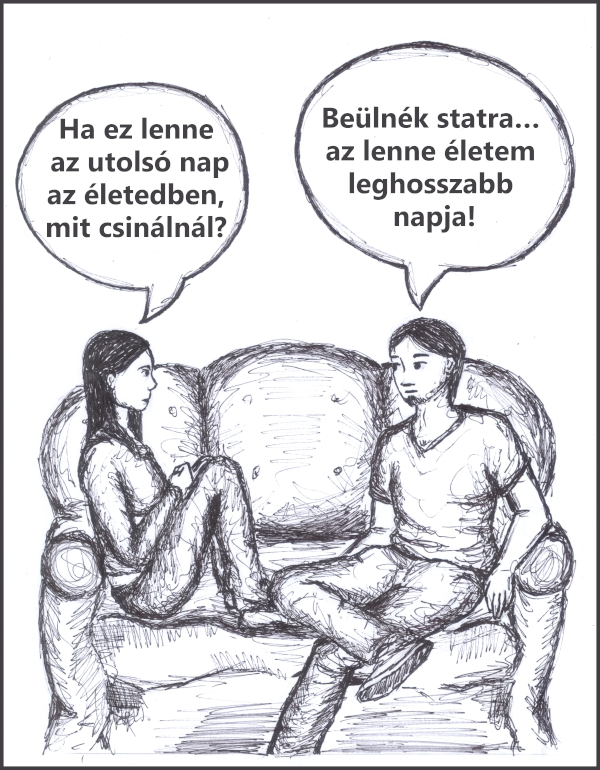
\includegraphics[width=0.7\linewidth]{images/ch_06_small} \end{center}

\hypertarget{beolvas-alapveto}{%
\section{Alapvető formátumok}\label{beolvas-alapveto}}

\begin{rmdlevel1}
Ebben a fejezetben áttekintjük:

\begin{itemize}
\tightlist
\item
  a táblázatkezelők állományainak beolvasását,
\item
  a tagolt szöveges állományok fogalmát és
\item
  azok beolvasását az \emph{Alap R}-ben.
\end{itemize}
\end{rmdlevel1}

Az R-ben adatokkal dolgozunk, amelyek beolvasására és kiírására az R számos eljárást kínál. Adatokat beolvashatunk a billentyűzetről, a vágóasztalról és külső adatforrásból, állományból vagy adatbázisból is. Az R-ben feldolgozott adatokat a vágóasztalra, adatbázisba vagy állományba írhatjuk ki. Ebben a fejezetben csak a két legtermészetesebb beolvasási módszert ismertetjük, az adatok beolvasást táblázatkezelők (pl. Microsoft Excel, LibreOffice Calc) állományaiból és tagolt szöveges állományokból.

\hypertarget{tuxe1bluxe1zatkezelux151k}{%
\subsection{Táblázatkezelők}\label{tuxe1bluxe1zatkezelux151k}}

A táblázatkezelők saját állományai (pl. \texttt{.xlsx} és \texttt{.ods}) kezelhetők a legkényelmesebben az adatelemzés során. Az adatbevitel és a rögzített adatok karbantartása, későbbi módosítása ebben a formátumban a legegyszerűbb, ráadásul a számítógépes tesztek sokszor ilyen típusú állományokba írják a válaszokat. Ezek az állományok (munkafüzetek) munkalapokból állnak, így akár több adatbázist is tárolhatunk egyetlen munkafüzetben. Egy Excel vagy LibreOffice Calc adatbázis esetén tudnunk kell, hogy az melyik munkalapon helyezkedik el, ritkábban pedig azt is, melyik tartományban foglal helyet a beolvasandó adatbázis.

Az Excel és LibreOffice Calc adatbázisok beolvasást a \textbf{rio} csomag \texttt{import()} függvényével végezzük, melynek egyetlen kötelező argumentuma a fájl elérési útja (\texttt{file=}).

Előkészítettünk egy 4 munkalapos Excel és LibreOffice Calc adatbázist (\texttt{agatha\_christie\_m.xlsx}, \texttt{agatha\_christie\_m.ods}), amelynek mindegyik munkalapján ugyanazt az adatbázist találjuk meg, de egyre zajosabb környezetben.

Az 1. munkalapon nincsenek zavaró cellák, csupán a adatbázisunk értékes adatcellái az \texttt{A1} cellától kezdődően.. Ebben az esetben nincs szükség más argumentumra, csak az állomány elérési útjára.

\begin{Shaded}
\begin{Highlighting}[]
\FunctionTok{library}\NormalTok{(rio)}
\NormalTok{ac}\FloatTok{.1} \OtherTok{\textless{}{-}} \FunctionTok{import}\NormalTok{(}\AttributeTok{file =} \StringTok{"adat/agatha\_christie\_m.xlsx"}\NormalTok{) }\CommentTok{\# MS Excel}
\FunctionTok{head}\NormalTok{(ac}\FloatTok{.1}\NormalTok{[}\DecValTok{1}\SpecialCharTok{:}\DecValTok{3}\NormalTok{], }\AttributeTok{n=}\DecValTok{3}\NormalTok{)}
\CommentTok{\#\textgreater{}   megjelenes.eve                  cim.magyar                  cim.angol}
\CommentTok{\#\textgreater{} 1           1930      Gyilkosság a paplakban The Murder at the Vicarage}
\CommentTok{\#\textgreater{} 2           1942 Holttest a könyvtárszobában    The Body in the Library}
\CommentTok{\#\textgreater{} 3           1942           A láthatatlan kéz          The Moving Finger}
\NormalTok{ac}\FloatTok{.1} \OtherTok{\textless{}{-}} \FunctionTok{import}\NormalTok{(}\AttributeTok{file =} \StringTok{"adat/agatha\_christie\_m.ods"}\NormalTok{)  }\CommentTok{\# LibreOffice Calc}
\FunctionTok{head}\NormalTok{(ac}\FloatTok{.1}\NormalTok{[}\DecValTok{1}\SpecialCharTok{:}\DecValTok{3}\NormalTok{], }\AttributeTok{n=}\DecValTok{3}\NormalTok{)}
\CommentTok{\#\textgreater{}   megjelenes.eve                  cim.magyar                  cim.angol}
\CommentTok{\#\textgreater{} 1           1930      Gyilkosság a paplakban The Murder at the Vicarage}
\CommentTok{\#\textgreater{} 2           1942 Holttest a könyvtárszobában    The Body in the Library}
\CommentTok{\#\textgreater{} 3           1942           A láthatatlan kéz          The Moving Finger}
\end{Highlighting}
\end{Shaded}

A 2. munkalapon már nem az \texttt{A1} cellában kezdődik az adatbázis, de továbbra sincs zavaró egyéb cella. Az \texttt{import()} megtalálja az adatbázist a munkalapon az Excel adatbázis esetében, de a LibreOffice Calc adatbázis beolvasásához pontosítani kell az adatbázis helyét. A tartomány közvetlen megadásával (\texttt{range="F7:I52"}) utasítjuk az \texttt{import()} függvényt, hogy honnan olvassa be az adatbázisunkat. Természetesen a megadott cellatartomány az oszlopneveket is tartalmazza annak első sorában.

Az \texttt{XLSX} és az \texttt{ODS} beolvasása közötti eltérés rávilágít az \texttt{import()} függvényünk működésére. Nem maga az \texttt{import()} végzi a közvetlen beolvasást, hanem okosan kiválasztja a beolvasandó állomány kiterjesztése alapján, hogy melyik csomag, melyik konkrét függvényét hívja. Az Excel állományokat a \emph{Tidyverse R} \textbf{readxl} csomag \texttt{read\_excel()} függvénye fogja beolvasni, a LibreOffice Calc állományokat a \textbf{readODS} csomag \texttt{read\_ods()} függvénye, amelyek hívását már az \texttt{import()} végzi. Mivel két különböző függvény dolgozik a háttérben, így az \texttt{XLSX} és az \texttt{ODS} állományokat beolvasó parancs paraméterezése is eltérhet, és esetünkben el is tér. A \texttt{file=} argumentum közös, és természetesen a munkalap sorszámát meg kell adnunk, amely mindkét esetben a \texttt{sheet=2}-vel történik.

\begin{Shaded}
\begin{Highlighting}[]
\NormalTok{ac}\FloatTok{.2} \OtherTok{\textless{}{-}} \FunctionTok{import}\NormalTok{(}\AttributeTok{file =} \StringTok{"adat/agatha\_christie\_m.xlsx"}\NormalTok{, }\AttributeTok{sheet=}\DecValTok{2}\NormalTok{)}
\FunctionTok{head}\NormalTok{(ac}\FloatTok{.2}\NormalTok{, }\AttributeTok{n=}\DecValTok{3}\NormalTok{)}
\CommentTok{\#\textgreater{}   megjelenes.eve                  cim.magyar                  cim.angol}
\CommentTok{\#\textgreater{} 1           1930      Gyilkosság a paplakban The Murder at the Vicarage}
\CommentTok{\#\textgreater{} 2           1942 Holttest a könyvtárszobában    The Body in the Library}
\CommentTok{\#\textgreater{} 3           1942           A láthatatlan kéz          The Moving Finger}
\CommentTok{\#\textgreater{}      szereplo}
\CommentTok{\#\textgreater{} 1 Miss Marple}
\CommentTok{\#\textgreater{} 2 Miss Marple}
\CommentTok{\#\textgreater{} 3 Miss Marple}
\NormalTok{ac}\FloatTok{.2} \OtherTok{\textless{}{-}} \FunctionTok{import}\NormalTok{(}\AttributeTok{file =} \StringTok{"adat/agatha\_christie\_m.ods"}\NormalTok{, }\AttributeTok{sheet=}\DecValTok{2}\NormalTok{, }\AttributeTok{range=}\StringTok{"F7:I52"}\NormalTok{)}
\FunctionTok{head}\NormalTok{(ac}\FloatTok{.2}\NormalTok{, }\AttributeTok{n=}\DecValTok{3}\NormalTok{)}
\CommentTok{\#\textgreater{}   megjelenes.eve                  cim.magyar                  cim.angol}
\CommentTok{\#\textgreater{} 1           1930      Gyilkosság a paplakban The Murder at the Vicarage}
\CommentTok{\#\textgreater{} 2           1942 Holttest a könyvtárszobában    The Body in the Library}
\CommentTok{\#\textgreater{} 3           1942           A láthatatlan kéz          The Moving Finger}
\CommentTok{\#\textgreater{}      szereplo}
\CommentTok{\#\textgreater{} 1 Miss Marple}
\CommentTok{\#\textgreater{} 2 Miss Marple}
\CommentTok{\#\textgreater{} 3 Miss Marple}
\end{Highlighting}
\end{Shaded}

A 3. munkalapon már az első 6 sor zavaró, nem az adatbázishoz tartozó adatokat tartalmaz, így azokat elegendő kihagyni (\texttt{skip=6}) a beolvasásból az Excel esetében, míg az \texttt{ODS}-hez a tartomány pontos megadása szükséges a sikeres beolvasásához.

\begin{Shaded}
\begin{Highlighting}[]
\NormalTok{ac}\FloatTok{.3} \OtherTok{\textless{}{-}} \FunctionTok{import}\NormalTok{(}\AttributeTok{file =} \StringTok{"adat/agatha\_christie\_m.xlsx"}\NormalTok{, }\AttributeTok{sheet=}\DecValTok{3}\NormalTok{, }\AttributeTok{skip=}\DecValTok{6}\NormalTok{)}
\FunctionTok{head}\NormalTok{(ac}\FloatTok{.3}\NormalTok{, }\AttributeTok{n=}\DecValTok{3}\NormalTok{)}
\CommentTok{\#\textgreater{}   megjelenes.eve                  cim.magyar                  cim.angol}
\CommentTok{\#\textgreater{} 1           1930      Gyilkosság a paplakban The Murder at the Vicarage}
\CommentTok{\#\textgreater{} 2           1942 Holttest a könyvtárszobában    The Body in the Library}
\CommentTok{\#\textgreater{} 3           1942           A láthatatlan kéz          The Moving Finger}
\CommentTok{\#\textgreater{}      szereplo}
\CommentTok{\#\textgreater{} 1 Miss Marple}
\CommentTok{\#\textgreater{} 2 Miss Marple}
\CommentTok{\#\textgreater{} 3 Miss Marple}
\NormalTok{ac}\FloatTok{.3} \OtherTok{\textless{}{-}} \FunctionTok{import}\NormalTok{(}\AttributeTok{file =} \StringTok{"adat/agatha\_christie\_m.ods"}\NormalTok{, }\AttributeTok{sheet=}\DecValTok{3}\NormalTok{, }\AttributeTok{range=}\StringTok{"F7:I52"}\NormalTok{)}
\FunctionTok{head}\NormalTok{(ac}\FloatTok{.3}\NormalTok{, }\AttributeTok{n=}\DecValTok{3}\NormalTok{)}
\CommentTok{\#\textgreater{}   megjelenes.eve                  cim.magyar                  cim.angol}
\CommentTok{\#\textgreater{} 1           1930      Gyilkosság a paplakban The Murder at the Vicarage}
\CommentTok{\#\textgreater{} 2           1942 Holttest a könyvtárszobában    The Body in the Library}
\CommentTok{\#\textgreater{} 3           1942           A láthatatlan kéz          The Moving Finger}
\CommentTok{\#\textgreater{}      szereplo}
\CommentTok{\#\textgreater{} 1 Miss Marple}
\CommentTok{\#\textgreater{} 2 Miss Marple}
\CommentTok{\#\textgreater{} 3 Miss Marple}
\end{Highlighting}
\end{Shaded}

A 4. munkalapon már rendkívül terhelt az adatbázisunk a környező zavaró celláktól, így közvetlenül a tartomány megadásával (\texttt{range="F7:I52"}) utasítjuk az \texttt{import()} függvényt Excel esetében is, hogy honnan olvassa be az adatbázisunkat.

\begin{Shaded}
\begin{Highlighting}[]
\NormalTok{ac}\FloatTok{.4} \OtherTok{\textless{}{-}} \FunctionTok{import}\NormalTok{(}\AttributeTok{file =} \StringTok{"adat/agatha\_christie\_m.xlsx"}\NormalTok{, }\AttributeTok{sheet=}\DecValTok{4}\NormalTok{, }\AttributeTok{range=}\StringTok{"F7:I52"}\NormalTok{)}
\FunctionTok{head}\NormalTok{(ac}\FloatTok{.4}\NormalTok{, }\AttributeTok{n=}\DecValTok{3}\NormalTok{)}
\CommentTok{\#\textgreater{}   megjelenes.eve                  cim.magyar                  cim.angol}
\CommentTok{\#\textgreater{} 1           1930      Gyilkosság a paplakban The Murder at the Vicarage}
\CommentTok{\#\textgreater{} 2           1942 Holttest a könyvtárszobában    The Body in the Library}
\CommentTok{\#\textgreater{} 3           1942           A láthatatlan kéz          The Moving Finger}
\CommentTok{\#\textgreater{}      szereplo}
\CommentTok{\#\textgreater{} 1 Miss Marple}
\CommentTok{\#\textgreater{} 2 Miss Marple}
\CommentTok{\#\textgreater{} 3 Miss Marple}
\NormalTok{ac}\FloatTok{.4} \OtherTok{\textless{}{-}} \FunctionTok{import}\NormalTok{(}\AttributeTok{file =} \StringTok{"adat/agatha\_christie\_m.ods"}\NormalTok{, }\AttributeTok{sheet=}\DecValTok{4}\NormalTok{, }\AttributeTok{range=}\StringTok{"F7:I52"}\NormalTok{)}
\FunctionTok{head}\NormalTok{(ac}\FloatTok{.4}\NormalTok{, }\AttributeTok{n=}\DecValTok{3}\NormalTok{)}
\CommentTok{\#\textgreater{}   megjelenes.eve                  cim.magyar                  cim.angol}
\CommentTok{\#\textgreater{} 1           1930      Gyilkosság a paplakban The Murder at the Vicarage}
\CommentTok{\#\textgreater{} 2           1942 Holttest a könyvtárszobában    The Body in the Library}
\CommentTok{\#\textgreater{} 3           1942           A láthatatlan kéz          The Moving Finger}
\CommentTok{\#\textgreater{}      szereplo}
\CommentTok{\#\textgreater{} 1 Miss Marple}
\CommentTok{\#\textgreater{} 2 Miss Marple}
\CommentTok{\#\textgreater{} 3 Miss Marple}
\end{Highlighting}
\end{Shaded}

Jegyezzük meg, ha csak tehetjük, adatainkat táblázatkezelő programmal hozzuk létre és annak saját formátumában (\texttt{XLSX} vagy \texttt{ODS}) tároljuk.

\hypertarget{tagolt-szuxf6veges-uxe1llomuxe1nyok}{%
\subsection{Tagolt szöveges állományok}\label{tagolt-szuxf6veges-uxe1llomuxe1nyok}}

A tagolt szöveges állományok kitüntetett szerepet játszanak a statisztikai adatfeldolgozásban, ugyanis minden statisztikai programcsomag és táblázatkezelő be tud olvasni ilyen formátumú állományokat, és ki tud exportálni ilyen formátumba. A tagolt szöveges állományok létrehozásához pedig egy jegyzettömbszerű szövegszerkesztő is elegendő, tehát ez a formátum elég nagy szabadságot ad az adataink kezeléshez.

\hypertarget{tagolt-szuxf6veges-uxe1llomuxe1ny-luxe9trehozuxe1sa}{%
\subsubsection{Tagolt szöveges állomány létrehozása}\label{tagolt-szuxf6veges-uxe1llomuxe1ny-luxe9trehozuxe1sa}}

A tagolt szöveges állomány egy egyszerű, formázást nem tartalmazó szöveges állomány, amelyet azonos szerkezetű sorok alkotnak. A sorokat az operációs rendszernek megfelelő sorvége karakterek zárják. Jegyzettömbszerű szövegszerkesztő használata során, az \texttt{ENTER} leütésével ezek a sorvége karakterek kerülnek fizikailag a szöveges állományba. Linux és macOS operációs rendszer alatt az \texttt{LF} karakter, Windows platformon a \texttt{CR} és \texttt{LF} karakterek. Ezeket sorvége karaktereknek hívjuk, az \texttt{LF} a soremelés (\texttt{\textbackslash{}n}), a \texttt{CR} a kocsi vissza (\texttt{\textbackslash{}r}) karakter. Annak ellenére, hogy különböző platformokon más-más jelzi a sorvégét, a beolvasó függvények felismerik ezeket, és helyesen értelmezik. Ezzel nekünk nem kell külön foglalkoznunk.

Minden tagolt szöveges állományban van egy kitüntetett karakter, a tagoló karakter. Ez tipikusan a pontosvessző (\texttt{;}), a szóköz (\texttt{}), a tabulátor (\texttt{\textbackslash{}t}) vagy a vessző (\texttt{,}) karakter. A tagolt szöveges állomány minden sorában ezek egyikét használjuk az adatértékek elválasztására, ráadásul minden sorban azonos számú adatértéknek kell szerepelni, ennek megfelelően minden sorban azonos számú tagoló karakter van.

Nézzünk példát pontosvesszővel tagolt szöveges állományra:

\begin{Shaded}
\begin{Highlighting}[]
\NormalTok{nem;kor;pulzus}
\NormalTok{fiú;12;71}
\NormalTok{fiú;11;69}
\NormalTok{lány;14;70}
\end{Highlighting}
\end{Shaded}

Összesen 4 sora van, soronként 3 adatértékkel, és 2 pontosvesszővel. Látható, hogy az első sor kitüntetett, azaz igazából nem méréssel kapott adatokat tartalmaz, hanem megnevezi azokat. Gyakori, hogy a tagolt szöveges állományok első sora ilyen speciális fejlécsor, amely tehát oszlopneveket tartalmaz. Ez nem kötelező, elképzelhető, hogy az első sorban már közvetlenül adatértékek vannak.

Nézzünk egy szóközzel tagolt szöveges állományt:

\begin{Shaded}
\begin{Highlighting}[]
\NormalTok{nem kor pulzus atlag}
\NormalTok{fiú 12 71 3,92}
\NormalTok{fiú 11 69 4,12}
\NormalTok{lány 14 70 5,00}
\end{Highlighting}
\end{Shaded}

Ez a tagolt szöveges állomány 4 sort, soronként 4 adatértéket és 3 elválasztó szóközt tartalmaz. Az első sora fejlécsor. Látható, hogy tizedes törtek is szerepelnek az állományban, a tizedesvesszőt valóban vesszővel jelöltük. Ez nem minden esetben van így, tizedes pont is elválaszthatná az egész és tört részt.

Tekintsünk egy elsőre kicsit rendezetlen szöveges állományt:

\begin{Shaded}
\begin{Highlighting}[]
\NormalTok{Általános iskolai felmérés}
\NormalTok{2019.03.02.}

\NormalTok{\#2.b}
\NormalTok{nem,kor,pulzus,atlag}
\NormalTok{fiú,12,71,3.92}
\NormalTok{\#fiú,11,69,4.12}
\NormalTok{lány,14,70,5.00 \# ellenőrizni}
\end{Highlighting}
\end{Shaded}

Az állomány második felében valóban felfedezhetjük a rendezettséget, a fejlécet 4 oszlopnévvel, és alatta a sorokat 4-4 adatértékkel. Ez a rész olyan, mint egy vesszővel elválasztott szöveges állomány, ahol a tizedes törtekben pontot használunk az egész és tört rész elválasztására.

Az állomány eleje azonban egyáltalán nem hasonlít a tagolt szöveges állományokra, és ráadásul kettős kereszttel (\texttt{\#}), vagyis megjegyzésnek szánt szövegekkel tarkított soraink is vannak. Az ilyen szabadabb stílusú állományok is beolvashatók az R-be, csupán meg kell adnunk, hogy az elejéről hány sort hagyjon figyelmen kívül (3 sort), és mit tekintsen megjegyzésnek (a kettős keresztet) a beolvasását végző eljárás. Ebben az esetben a fejlécen kívül még 2 adatsor lesz a beolvasott adattáblában.

Melyek a tagolt szöveges állományok fontos jellemzői:

\begin{itemize}
\tightlist
\item
  a tagoló karakter,
\item
  a decimális elválasztó,
\item
  van-e fejlécsor,
\item
  hány sort lépjünk át az elejéről,
\item
  mi a megjegyzés karakter,
\item
  milyen kódolású az állomány.
\end{itemize}

Ahogyan említettük tagolt szöveges állományt egy jegyzettömbszerű szövegszerkesztővel mi is létrehozhatunk, de ha módunk van rá, akkor a minél kényelmesebb adatbevitel miatt, használjunk táblázatkezelőt, és az abban elkészült táblázatos formában lévő adatokat exportáljuk ki tagolt szöveges állományba. Például magyar Excel esetén választhatjuk a \texttt{CSV\ (pontosvesszővel\ tagolt)}, vagy a \texttt{Szöveges\ (tabulátorral\ tagolt)} formátumot. Érdemes minden esetben megőrizni a táblázatkezelő saját formátumában az adatokat, mert a kényelmes szerkesztés miatt továbbra is abban érdemes az adatokat módosítani, de a változtatások után, utolsó lépésként, végezzük el az exportot a tagolt szöveges állományba.

\hypertarget{a-read.table-csaluxe1d}{%
\subsubsection{\texorpdfstring{A \texttt{read.table()} család}{A read.table() család}}\label{a-read.table-csaluxe1d}}

Tagolt szöveges állományok beolvasásának hagyományos módja a \texttt{read.table()} függvénycsalád használata. Azért nevezzük függvénycsaládnak, mert valójában több függvényt használhatunk, amelyek csak a paraméterek alapértelmezett értékében térnek el egymástól:

\begin{itemize}
\tightlist
\item
  \texttt{read.table(sep="",\ dec=".")},
\item
  \texttt{read.csv(sep=",",\ dec=".")},
\item
  \texttt{read.csv2(sep=";",\ dec=",")},
\item
  \texttt{read.delim(sep="\textbackslash{}t",\ dec=".")},
\item
  \texttt{read.delim2(sep="\textbackslash{}t",\ dec=",")}.
\end{itemize}

Érdemes a fenti függvénynevek megtanulása helyett egyetlen függvényt, a \texttt{read.table()}-t használni, és inkább a lehetséges paraméterek jelentését tanuljuk meg:

\begin{itemize}
\tightlist
\item
  \texttt{file=}\strut \\
  A beolvasandó állomány elérési útja.
\item
  \texttt{sep=}\strut \\
  Az elválasztó karakter a beolvasandó állományban. Tipikus értékei: \texttt{sep=";"}, \texttt{sep="\ "}, \texttt{sep=","}, és tabulátor elválasztó esetén \texttt{sep="\textbackslash{}t"}.
\item
  \texttt{dec=}\strut \\
  A decimális elválasztó, vagyis a tizedesvessző alakja az állományban. Tipikusan a \texttt{dec=","} beállítást kell használnunk, de előfordulhat, hogy a pont a tizedes elválasztó, így a \texttt{dec="."}-ra van szükségünk.
\item
  \texttt{header=}\strut \\
  Ha van fejléc a szöveges állományban, akkor \texttt{header=TRUE}, egyébként a \texttt{header=FALSE} beállítást használjuk.
\item
  \texttt{na.strings=}\strut \\
  A hiányzó érték jelölése a szöveges állományban. Az alapértelmezett beállítás a legtöbb esetben megfelelő, hiszen a \texttt{""} (semmi) és az \texttt{"NA"} jelölésből alapértelmezés szerint hiányzó érték lesz.
\item
  \texttt{comment.char=}\strut \\
  A tipikus megjegyzés karakter a \texttt{\#}, de meg tudjuk változtatni, ha szükséges.
\item
  \texttt{skip=}\strut \\
  A szöveges állomány első néhány sorát figyelmen kívül hagyhatjuk.
\item
  \texttt{stringsAsFactors=}\strut \\
  A \texttt{stringsAsFactors=TRUE} beállítással elérhetjük a karakteres oszlopok automatikus faktorrá konvertálását.
\item
  \texttt{fileEncoding=}\strut \\
  A szöveges állományt alkotó karakterek kódolási szabványát adhatjuk meg. Tipikusan az UTF-8 kódolású szöveges állományok beolvasása során kell használnunk (\texttt{fileEncoding="UTF-8"}), de a magyar környezetben készült szöveges állományok esetében is rögzíthetjük a kódolási szabványt (\texttt{fileEncoding="latin2"}).
\item
  \texttt{strip.white=}\strut \\
  A felesleges szóközök és tabulátorok eltávolítása az adatok elejéről és végéről.
\item
  \texttt{quote=}\strut \\
  A szöveges állományban lévő adatvédő idézőjelek alakja.
\end{itemize}

Végezzük el az \texttt{egyetem.csv} tagolt szöveges állomány beolvasását, amelynek első néhány sora a következő:

\begin{Shaded}
\begin{Highlighting}[]
\NormalTok{hallgato;Height;neme;lefekves;felkeles;Drink}
\NormalTok{1;67;female;{-}2,5;5,5;víz}
\NormalTok{2;64;female;1,5;8;üdítő}
\NormalTok{3;61;female;{-}1,5;7,5;tej}
\end{Highlighting}
\end{Shaded}

A beolvasandó állományunk egy első sorában oszlopneveket tartalmazó szöveges állomány, amelynek a tartalmát a következő parancsok egy \texttt{d.df} adattáblában helyezik el. Az állományban az adatokat (és az oszlopneveket is) a pontosvessző (\texttt{;}) választja el, a numerikus értékekben pedig tizedesvessző szerepel.

\begin{Shaded}
\begin{Highlighting}[]
\NormalTok{data.file }\OtherTok{\textless{}{-}} \StringTok{"https://github.com/abarik/rdata/raw/master/r\_alapok/egyetem.csv"}
\NormalTok{d.df }\OtherTok{\textless{}{-}} \FunctionTok{read.table}\NormalTok{(}\AttributeTok{file =}\NormalTok{ data.file, }\AttributeTok{header=}\NormalTok{T, }
                                     \AttributeTok{sep=}\StringTok{";"}\NormalTok{, }
                                     \AttributeTok{dec=}\StringTok{","}\NormalTok{, }
                                     \AttributeTok{strip.white =}\NormalTok{ T, }
                                     \AttributeTok{stringsAsFactors =}\NormalTok{ F, }
                                     \AttributeTok{fileEncoding =} \StringTok{"latin2"}\NormalTok{)}
\FunctionTok{str}\NormalTok{(d.df)}
\CommentTok{\#\textgreater{} \textquotesingle{}data.frame\textquotesingle{}:    657 obs. of  6 variables:}
\CommentTok{\#\textgreater{}  $ hallgato: int  1 2 3 4 5 6 7 8 9 10 ...}
\CommentTok{\#\textgreater{}  $ Height  : num  67 64 61 61 70 63 61 64 66 65 ...}
\CommentTok{\#\textgreater{}  $ neme    : chr  "female" "female" "female" "female" ...}
\CommentTok{\#\textgreater{}  $ lefekves: num  {-}2.5 1.5 {-}1.5 2 0 1 1.5 0.5 {-}0.5 2.5 ...}
\CommentTok{\#\textgreater{}  $ felkeles: num  5.5 8 7.5 8.5 9 8.5 7.5 7.5 7 8.5 ...}
\CommentTok{\#\textgreater{}  $ Drink   : chr  "víz" "üdítő" "tej" "víz" ...}
\end{Highlighting}
\end{Shaded}

\hypertarget{beolvasas-1-summary}{%
\subsection{Összefoglalás}\label{beolvasas-1-summary}}

\begin{rmdsummary}
A statisztikai munka első lépése az adatbázisok, adatmátrixok
beolvasása. Adatainkat legkényelmesebb Excel vagy LibreOffice Calc
táblázatkezelők saját formátumú adatállományiban tárolni (\texttt{XLSX},
\texttt{ODS}), de néha nem kerülhetjük el a tagolt szöveges állományok
használatát. A táblázatkezelők adatállományait a \textbf{rio} csomag
\texttt{import()} függvényével olvashatjuk be, a tagolt szöveges
állományokat a \texttt{read.table()} függvénnyel.
\end{rmdsummary}

\hypertarget{beolvasas-1-exercise}{%
\subsection{Feladatok}\label{beolvasas-1-exercise}}

\begin{rmdexercise}
\begin{enumerate}
\def\labelenumi{\arabic{enumi}.}
\tightlist
\item
  Olvassuk be a \texttt{https://onlinestatbook.com/2/case\_studies/data/leniency.xls} Excel állományt, állapítsuk meg hány sora és oszlopa van.
\item
  Olvassuk be a \texttt{https://vincentarelbundock.github.io/Rdatasets/csv/DAAG/socsupport.csv} tagolt szöveges állományt, állapítsuk meg hány sora és oszlopa van.
\end{enumerate}
\end{rmdexercise}

\hypertarget{a-tidyverse-r-uxe9s-az-inline-beolvasuxe1s}{%
\section{A Tidyverse R és az inline beolvasás}\label{a-tidyverse-r-uxe9s-az-inline-beolvasuxe1s}}

\begin{rmdlevel2}
Ebben a fejezetben áttekintjük

\begin{itemize}
\tightlist
\item
  az inline beolvasás eseteit és
\item
  a tagolt szöveges állományok \emph{Tidyverse R} beolvasását.
\end{itemize}
\end{rmdlevel2}

\hypertarget{a-read_delim-fuxfcggvuxe9nycsaluxe1d}{%
\subsection{\texorpdfstring{A \texttt{read\_delim()} függvénycsalád}{A read\_delim() függvénycsalád}}\label{a-read_delim-fuxfcggvuxe9nycsaluxe1d}}

A \emph{Tidyverse R} is képes a tagolt szöveges állományok beolvasására, és rendszerint gyorsabb, jobban paraméterezhető lehetőséget nyújt. Lényeges különbség az előző részben látott \texttt{read.table()} családhoz képest, hogy minden esetben \emph{tibble} típusú adattábla a beolvasás eredménye.

A \texttt{read\_delim()} család tagjai:

\begin{itemize}
\tightlist
\item
  \texttt{read\_delim()},
\item
  \texttt{read\_csv},
\item
  \texttt{read\_csv2},
\item
  \texttt{read\_tsv}.
\end{itemize}

Minden esetben használjuk a \texttt{read\_delim()} függvényt, amely nagyon hasonló paraméterekkel rendelkezik, mint a \texttt{read.table()}:

\begin{itemize}
\tightlist
\item
  \texttt{file=}\strut \\
  Ugyanaz, mint a \texttt{read.table()} függvénynél.
\item
  \texttt{delim=}\strut \\
  Ugyanaz, mint a \texttt{read.table()} függvénynél a \texttt{sep=} argumentum.
\item
  \texttt{locale=}\strut \\
  A decimális elválasztó és a kódolási szabvány beállításához a \texttt{locale()} függvényt használjuk. Ha a szokásos vessző a tizedes vessző alakja, akkor a \texttt{locale\ =\ locale(decimal\_mark\ =\ ",")}, egyébként a \texttt{locale\ =\ locale(decimal\_mark\ =\ ".")} beállítást használjuk. Ha a kódolási szabványt is be szeretnénk állítani a vessző decimális elválasztó mellett, akkor a \texttt{locale\ =\ locale(decimal\_mark\ =\ ".",\ encoding\ =\ "UTF-8")} beállításra van szükségünk az UTF-8 beállításához.
\item
  \texttt{col\_names=}\strut \\
  Ugyanaz, mint a \texttt{read.table()} függvénynél a \texttt{header=} argumentum.
\item
  \texttt{na=}\strut \\
  Ugyanaz, mint a \texttt{read.table()} függvénynél a \texttt{na.strings=} argumentum.
\item
  \texttt{comment=}\strut \\
  Ugyanaz, mint a \texttt{read.table()} függvénynél a \texttt{comment.char=} argumentum.
\item
  \texttt{skip=}\strut \\
  Ugyanaz, mint a \texttt{read.table()} függvénynél.
\item
  \texttt{trim\_ws}\strut \\
  Ugyanaz, mint a \texttt{read.table()} függvénynél a \texttt{strip.white=} argumentum.
\item
  \texttt{quote}\strut \\
  Ugyanaz, mint a \texttt{read.table()} függvénynél.
\end{itemize}

Végezzük el a már korábban megismert \texttt{egyetem.csv} tagolt szöveges állomány beolvasását a \emph{Tidyverse R} segítségével:

\begin{Shaded}
\begin{Highlighting}[]
\NormalTok{data.file }\OtherTok{\textless{}{-}} \StringTok{"https://github.com/abarik/rdata/raw/master/r\_alapok/egyetem.csv"}
\FunctionTok{library}\NormalTok{(tidyverse)}
\NormalTok{d.tbl }\OtherTok{\textless{}{-}} \FunctionTok{read\_delim}\NormalTok{(}\AttributeTok{file =}\NormalTok{ data.file, }\AttributeTok{col\_names=}\NormalTok{T, }
                                      \AttributeTok{delim=}\StringTok{";"}\NormalTok{, }
                                      \AttributeTok{locale=}\FunctionTok{locale}\NormalTok{(}\AttributeTok{decimal\_mark=}\StringTok{","}\NormalTok{, }\AttributeTok{encoding =} \StringTok{"latin2"}\NormalTok{), }
                                      \AttributeTok{trim\_ws=}\NormalTok{ T)}
\FunctionTok{str}\NormalTok{(d.tbl)}
\CommentTok{\#\textgreater{} spec\_tbl\_df [657 x 6] (S3: spec\_tbl\_df/tbl\_df/tbl/data.frame)}
\CommentTok{\#\textgreater{}  $ hallgato: num [1:657] 1 2 3 4 5 6 7 8 9 10 ...}
\CommentTok{\#\textgreater{}  $ Height  : num [1:657] 67 64 61 61 70 63 61 64 66 65 ...}
\CommentTok{\#\textgreater{}  $ neme    : chr [1:657] "female" "female" "female" "female" ...}
\CommentTok{\#\textgreater{}  $ lefekves: num [1:657] {-}2.5 1.5 {-}1.5 2 0 1 1.5 0.5 {-}0.5 2.5 ...}
\CommentTok{\#\textgreater{}  $ felkeles: num [1:657] 5.5 8 7.5 8.5 9 8.5 7.5 7.5 7 8.5 ...}
\CommentTok{\#\textgreater{}  $ Drink   : chr [1:657] "víz" "üdítő" "tej" "víz" ...}
\CommentTok{\#\textgreater{}  {-} attr(*, "spec")=}
\CommentTok{\#\textgreater{}   .. cols(}
\CommentTok{\#\textgreater{}   ..   hallgato = col\_double(),}
\CommentTok{\#\textgreater{}   ..   Height = col\_double(),}
\CommentTok{\#\textgreater{}   ..   neme = col\_character(),}
\CommentTok{\#\textgreater{}   ..   lefekves = col\_double(),}
\CommentTok{\#\textgreater{}   ..   felkeles = col\_double(),}
\CommentTok{\#\textgreater{}   ..   Drink = col\_character()}
\CommentTok{\#\textgreater{}   .. )}
\CommentTok{\#\textgreater{}  {-} attr(*, "problems")=\textless{}externalptr\textgreater{}}
\end{Highlighting}
\end{Shaded}

\hypertarget{inline-beolvasuxe1s}{%
\subsection{Inline beolvasás}\label{inline-beolvasuxe1s}}

Ebben a könyvben a külső adatállományokból való beolvasás mellet az inline adatbeolvasást is részletesen bemutatjuk. Kisebb adatbázisok, egyszerűbb adatfeldolgozás esetén az adatokat közvetlenül a parancsállományokban is elhelyezhetjük, ezt nevezzük \emph{sorok közötti}, vagy más néven \emph{inline} adatbeolvasásának. A szokásos eset azonban a külső adatállományból való adatbeolvasás.

Az adatok inline beolvasása azt jelenti, hogy nem külső állományból, hanem az R parancsállományba gépelt adatokból indulunk ki. Felhasználjuk a \texttt{c()}, \texttt{factor()} és a \texttt{data.frame()} függvényeket az \emph{Alap R}-ből, valamint a \texttt{tibble()} vagy \texttt{tribble()} függvényeket a \emph{Tidyverse R}-ből. Esetleg használhatjuk az állományok beolvasását végző, most megismert \texttt{read.table()} (\emph{Alap R}) és \texttt{read\_delim()} (\emph{Tidyverse R}) függvénycsaládokat is.

A legegyszerűbb adatfeldolgozási feladatok egyetlen változót érintenek, ezek pedig numerikus vektorban vagy faktorban tárolhatók az R-ben. Ez az inline beolvasás legegyszerűbb esete.

\begin{Shaded}
\begin{Highlighting}[]
\CommentTok{\# 4 óvodás testmagassága cm{-}ben}
\NormalTok{magassag }\OtherTok{\textless{}{-}} \FunctionTok{c}\NormalTok{(}\DecValTok{132}\NormalTok{, }\DecValTok{143}\NormalTok{, }\DecValTok{129}\NormalTok{, }\DecValTok{145}\NormalTok{)}
\FunctionTok{mean}\NormalTok{(magassag)  }\CommentTok{\# testmagasság átlaga}
\CommentTok{\#\textgreater{} [1] 137.2}
\CommentTok{\# a 4 óvodás neme}
\NormalTok{nem }\OtherTok{\textless{}{-}} \FunctionTok{factor}\NormalTok{(}\FunctionTok{c}\NormalTok{(}\StringTok{"fiú"}\NormalTok{, }\StringTok{"lány"}\NormalTok{, }\StringTok{"lány"}\NormalTok{, }\StringTok{"fiú"}\NormalTok{), }\AttributeTok{levels=}\FunctionTok{c}\NormalTok{(}\StringTok{"fiú"}\NormalTok{, }\StringTok{"lány"}\NormalTok{)) }
\FunctionTok{table}\NormalTok{(nem, }\AttributeTok{useNA =} \StringTok{"ifany"}\NormalTok{)  }\CommentTok{\# gyakorisági táblázat a nemre}
\CommentTok{\#\textgreater{} nem}
\CommentTok{\#\textgreater{}  fiú lány }
\CommentTok{\#\textgreater{}    2    2}
\end{Highlighting}
\end{Shaded}

Több változó tárolása esetén \emph{adattábla} (\emph{data frame}) vagy \emph{tibble} típusú objektumot hozunk létre a korábban már megismert \texttt{data.frame()} és \texttt{tibble()} függvények segítségével. Előkészítő lépésként természetesen az oszlopokat alkotó vektorokra is szükség van.

\begin{Shaded}
\begin{Highlighting}[]
\FunctionTok{library}\NormalTok{(tidyverse)}
\NormalTok{magassag }\OtherTok{\textless{}{-}} \FunctionTok{c}\NormalTok{(}\DecValTok{132}\NormalTok{, }\DecValTok{143}\NormalTok{, }\DecValTok{129}\NormalTok{, }\DecValTok{145}\NormalTok{)}
\NormalTok{nem }\OtherTok{\textless{}{-}} \FunctionTok{factor}\NormalTok{(}\FunctionTok{c}\NormalTok{(}\StringTok{"fiú"}\NormalTok{, }\StringTok{"lány"}\NormalTok{, }\StringTok{"lány"}\NormalTok{, }\StringTok{"fiú"}\NormalTok{), }\AttributeTok{levels=}\FunctionTok{c}\NormalTok{(}\StringTok{"fiú"}\NormalTok{, }\StringTok{"lány"}\NormalTok{)) }
\NormalTok{d.df  }\OtherTok{\textless{}{-}} \FunctionTok{data.frame}\NormalTok{(magassag, nem) }\CommentTok{\# data frame létrehozása}
\NormalTok{d.tbl }\OtherTok{\textless{}{-}} \FunctionTok{tibble}\NormalTok{(magassag, nem)     }\CommentTok{\# tibble létrehozása}
\end{Highlighting}
\end{Shaded}

A létrehozott adattáblák is nagyon hasonlítanak egymásra, és felhasználásuk is azonos módon történik:

\begin{Shaded}
\begin{Highlighting}[]
\NormalTok{d.df    }\CommentTok{\# data frame}
\CommentTok{\#\textgreater{}   magassag  nem}
\CommentTok{\#\textgreater{} 1      132  fiú}
\CommentTok{\#\textgreater{} 2      143 lány}
\CommentTok{\#\textgreater{} 3      129 lány}
\CommentTok{\#\textgreater{} 4      145  fiú}
\NormalTok{d.tbl   }\CommentTok{\# tibble}
\CommentTok{\#\textgreater{} \# A tibble: 4 x 2}
\CommentTok{\#\textgreater{}   magassag nem  }
\CommentTok{\#\textgreater{}      \textless{}dbl\textgreater{} \textless{}fct\textgreater{}}
\CommentTok{\#\textgreater{} 1      132 fiú  }
\CommentTok{\#\textgreater{} 2      143 lány }
\CommentTok{\#\textgreater{} 3      129 lány }
\CommentTok{\#\textgreater{} 4      145 fiú}
\FunctionTok{mean}\NormalTok{(d.df}\SpecialCharTok{$}\NormalTok{magassag)                }\CommentTok{\# testmagasság átlaga}
\CommentTok{\#\textgreater{} [1] 137.2}
\FunctionTok{mean}\NormalTok{(d.tbl}\SpecialCharTok{$}\NormalTok{magassag)               }\CommentTok{\# testmagasság átlaga}
\CommentTok{\#\textgreater{} [1] 137.2}
\FunctionTok{table}\NormalTok{(d.df}\SpecialCharTok{$}\NormalTok{nem, }\AttributeTok{useNA =} \StringTok{"ifany"}\NormalTok{)   }\CommentTok{\# gyakorisági táblázat a nemre}
\CommentTok{\#\textgreater{} }
\CommentTok{\#\textgreater{}  fiú lány }
\CommentTok{\#\textgreater{}    2    2}
\FunctionTok{table}\NormalTok{(d.tbl}\SpecialCharTok{$}\NormalTok{nem, }\AttributeTok{useNA =} \StringTok{"ifany"}\NormalTok{)  }\CommentTok{\# gyakorisági táblázat a nemre}
\CommentTok{\#\textgreater{} }
\CommentTok{\#\textgreater{}  fiú lány }
\CommentTok{\#\textgreater{}    2    2}
\end{Highlighting}
\end{Shaded}

Nem kell feltétlenül az adattáblát alkotó oszlopokat külön numerikus vagy faktor oszlopokban előzőleg elkészíteni, ezeket a \texttt{data.frame()} vagy \texttt{tibble()} argumentumába közvetlenül is beírhatjuk:

\begin{Shaded}
\begin{Highlighting}[]
\NormalTok{d.df }\OtherTok{\textless{}{-}} \FunctionTok{data.frame}\NormalTok{(}
  \AttributeTok{magassag =} \FunctionTok{c}\NormalTok{(}\DecValTok{132}\NormalTok{, }\DecValTok{143}\NormalTok{, }\DecValTok{129}\NormalTok{, }\DecValTok{145}\NormalTok{),}
  \AttributeTok{nem =} \FunctionTok{factor}\NormalTok{(}\FunctionTok{c}\NormalTok{(}\StringTok{"fiú"}\NormalTok{, }\StringTok{"lány"}\NormalTok{, }\StringTok{"lány"}\NormalTok{, }\StringTok{"fiú"}\NormalTok{), }\AttributeTok{levels=}\FunctionTok{c}\NormalTok{(}\StringTok{"fiú"}\NormalTok{, }\StringTok{"lány"}\NormalTok{)) }
\NormalTok{)}

\NormalTok{d.tbl }\OtherTok{\textless{}{-}} \FunctionTok{tibble}\NormalTok{(}
  \AttributeTok{magassag =} \FunctionTok{c}\NormalTok{(}\DecValTok{132}\NormalTok{, }\DecValTok{143}\NormalTok{, }\DecValTok{129}\NormalTok{, }\DecValTok{145}\NormalTok{),}
  \AttributeTok{nem =} \FunctionTok{factor}\NormalTok{(}\FunctionTok{c}\NormalTok{(}\StringTok{"fiú"}\NormalTok{, }\StringTok{"lány"}\NormalTok{, }\StringTok{"lány"}\NormalTok{, }\StringTok{"fiú"}\NormalTok{), }\AttributeTok{levels=}\FunctionTok{c}\NormalTok{(}\StringTok{"fiú"}\NormalTok{, }\StringTok{"lány"}\NormalTok{)) }
\NormalTok{)}
\end{Highlighting}
\end{Shaded}

Tibble létrehozásának másik módja a \texttt{tribble()} függvény, amelynek argumentumába táblázatos formában adhatjuk meg az adatokat. A változóneveket a \texttt{\textasciitilde{}} karakter vezeti be, minden adatértéket és oszlopnevet vessző választ el egymástól a \texttt{tribble()} argumentumában.

\begin{Shaded}
\begin{Highlighting}[]
\NormalTok{d.tbl }\OtherTok{\textless{}{-}} \FunctionTok{tribble}\NormalTok{(}
  \SpecialCharTok{\textasciitilde{}}\NormalTok{magassag,  }\SpecialCharTok{\textasciitilde{}}\NormalTok{nem,}
  \DecValTok{132}\NormalTok{, }\StringTok{"fiú"}\NormalTok{,}
  \DecValTok{143}\NormalTok{, }\StringTok{"lány"}\NormalTok{,}
  \DecValTok{129}\NormalTok{, }\StringTok{"lány"}\NormalTok{,}
  \DecValTok{145}\NormalTok{, }\StringTok{"fiú"}
\NormalTok{)}
\NormalTok{d.tbl}
\CommentTok{\#\textgreater{} \# A tibble: 4 x 2}
\CommentTok{\#\textgreater{}   magassag nem  }
\CommentTok{\#\textgreater{}      \textless{}dbl\textgreater{} \textless{}chr\textgreater{}}
\CommentTok{\#\textgreater{} 1      132 fiú  }
\CommentTok{\#\textgreater{} 2      143 lány }
\CommentTok{\#\textgreater{} 3      129 lány }
\CommentTok{\#\textgreater{} 4      145 fiú}
\end{Highlighting}
\end{Shaded}

Vegyük észre, hogy a \texttt{nem} oszlop a fenti példában karakteres vektor, a faktorrá alakításáról a \texttt{factor()} függvénnyel gondoskodnunk kell.

\begin{Shaded}
\begin{Highlighting}[]
\NormalTok{d.tbl}\SpecialCharTok{$}\NormalTok{nem }\OtherTok{\textless{}{-}} \FunctionTok{factor}\NormalTok{(d.tbl}\SpecialCharTok{$}\NormalTok{nem, }\AttributeTok{levels=}\FunctionTok{c}\NormalTok{(}\StringTok{"fiú"}\NormalTok{, }\StringTok{"lány"}\NormalTok{)) }
\NormalTok{d.tbl}
\CommentTok{\#\textgreater{} \# A tibble: 4 x 2}
\CommentTok{\#\textgreater{}   magassag nem  }
\CommentTok{\#\textgreater{}      \textless{}dbl\textgreater{} \textless{}fct\textgreater{}}
\CommentTok{\#\textgreater{} 1      132 fiú  }
\CommentTok{\#\textgreater{} 2      143 lány }
\CommentTok{\#\textgreater{} 3      129 lány }
\CommentTok{\#\textgreater{} 4      145 fiú}
\end{Highlighting}
\end{Shaded}

A \texttt{read.table()} és \texttt{read\_delim()} függvénycsaládokat is használhatjuk inline beolvasásra. Mindkét esetben egy inline, szóközzel tagolt szöveges állományt illesztettünk a kódba, ennek megfelelően állítottuk be az elválasztó karaktereket. A \texttt{read.table()} esetében körbevettük a \texttt{textConnection()} függvénnyel is a beillesztett adatokat, erre a \emph{Tidyverse R} \texttt{read\_delim()}-jénél már nincs szükség. A \texttt{nem} faktorrá konvertálásáról se felejtkezzünk el.

\begin{Shaded}
\begin{Highlighting}[]
\NormalTok{d.df }\OtherTok{\textless{}{-}} \FunctionTok{read.table}\NormalTok{(}\AttributeTok{file =} \FunctionTok{textConnection}\NormalTok{(}\StringTok{"}
\StringTok{magassag nem}
\StringTok{132 fiú}
\StringTok{143 lány}
\StringTok{129 lány}
\StringTok{145 fiú}
\StringTok{"}\NormalTok{), }\AttributeTok{header=}\NormalTok{T, }\AttributeTok{sep=}\StringTok{" "}\NormalTok{)}
\NormalTok{d.df}\SpecialCharTok{$}\NormalTok{nem }\OtherTok{\textless{}{-}} \FunctionTok{factor}\NormalTok{(d.df}\SpecialCharTok{$}\NormalTok{nem, }\AttributeTok{levels=}\FunctionTok{c}\NormalTok{(}\StringTok{"fiú"}\NormalTok{, }\StringTok{"lány"}\NormalTok{)) }
\NormalTok{d.df}
\CommentTok{\#\textgreater{}   magassag  nem}
\CommentTok{\#\textgreater{} 1      132  fiú}
\CommentTok{\#\textgreater{} 2      143 lány}
\CommentTok{\#\textgreater{} 3      129 lány}
\CommentTok{\#\textgreater{} 4      145  fiú}
\NormalTok{d.tbl }\OtherTok{\textless{}{-}} \FunctionTok{read\_delim}\NormalTok{(}\StringTok{"}
\StringTok{magassag nem}
\StringTok{132 fiú}
\StringTok{143 lány}
\StringTok{129 lány}
\StringTok{145 fiú}
\StringTok{"}\NormalTok{, }\AttributeTok{col\_names=}\NormalTok{T, }\AttributeTok{delim=}\StringTok{" "}\NormalTok{)}
\NormalTok{d.tbl}\SpecialCharTok{$}\NormalTok{nem }\OtherTok{\textless{}{-}} \FunctionTok{factor}\NormalTok{(d.tbl}\SpecialCharTok{$}\NormalTok{nem, }\AttributeTok{levels=}\FunctionTok{c}\NormalTok{(}\StringTok{"fiú"}\NormalTok{, }\StringTok{"lány"}\NormalTok{)) }
\NormalTok{d.tbl}
\CommentTok{\#\textgreater{} \# A tibble: 4 x 2}
\CommentTok{\#\textgreater{}   magassag nem  }
\CommentTok{\#\textgreater{}      \textless{}dbl\textgreater{} \textless{}fct\textgreater{}}
\CommentTok{\#\textgreater{} 1      132 fiú  }
\CommentTok{\#\textgreater{} 2      143 lány }
\CommentTok{\#\textgreater{} 3      129 lány }
\CommentTok{\#\textgreater{} 4      145 fiú}
\end{Highlighting}
\end{Shaded}

\hypertarget{beolvasas-2-summary}{%
\subsection{Összefoglalás}\label{beolvasas-2-summary}}

\begin{rmdsummary}
swwwww
\end{rmdsummary}

\hypertarget{beolvasas-2-exercise}{%
\subsection{Feladatok}\label{beolvasas-2-exercise}}

\begin{rmdexercise}
sadadasda
\end{rmdexercise}

\hypertarget{kiuxedruxe1s-uxe9s-muxe1s-lehetux151suxe9gek}{%
\section{Kiírás és más lehetőségek}\label{kiuxedruxe1s-uxe9s-muxe1s-lehetux151suxe9gek}}

\begin{rmdlevel3}
Ebben a fejezetben áttekintjük

\begin{itemize}
\tightlist
\item
  a tagolt szöveges állományok kiírását
\item
  objektumok olvasását és írását bináris állományokba,
\item
  más statisztikai programcsomagok adatállományainak olvasását és írását, és
\item
  a fix széles mezővel rendelkező állományok olvasását.
\end{itemize}
\end{rmdlevel3}

\hypertarget{tagolt-szuxf6veges-uxe1llomuxe1ny-kiuxedruxe1sa}{%
\subsection{Tagolt szöveges állomány kiírása}\label{tagolt-szuxf6veges-uxe1llomuxe1ny-kiuxedruxe1sa}}

Adattáblák és mátrixok kiírására a \texttt{write.table()}\index{write.table()} függvényt használhatjuk az \emph{Alap R}-ből és a \texttt{write\_delim()} függvényt a \emph{Tidyverse R}-ből. Mindkét függvény egy-egy függvénycsalád reprezentánsa, de az \emph{Alap R}-ből elegendő ismerni az említett tagot, a \emph{Tidyverse R}-ből pedig az említetten kívül a \texttt{write\_csv2()} függvényt. Néhány új argumentummal kell megismerkednünk, a korábban tanult argumentumok jelentését még egyszer nem soroljuk fel.

A \texttt{write.table()} mátrixok és adattáblák kiírására is alkalmas, míg a \texttt{write\_delim()} és a \texttt{write\_csv2()} csak az adattáblákat rögzíti. Az első paraméter (\texttt{x=}) a kiírandó objektum neve mindhárom függvény esetében.

Az első példában a \texttt{write.table()} függvénnyel egy mátrixot és a korábban létrehozott \texttt{d.df} adattáblát írjuk ki. A \texttt{row.names=} és a \texttt{col.names=} logikai paraméterek szabályozzák, hogy a sor és oszlopnevek szerepeljenek-e a kimeneti állományban. Ezek alapértelmezett értéke \texttt{TRUE}.

\begin{Shaded}
\begin{Highlighting}[]
\NormalTok{x.mat }\OtherTok{\textless{}{-}} \FunctionTok{matrix}\NormalTok{(}\DecValTok{1}\SpecialCharTok{:}\DecValTok{12}\NormalTok{, }\AttributeTok{nrow=}\DecValTok{3}\NormalTok{)                              }\CommentTok{\# mátrix létrehozása}
\FunctionTok{write.table}\NormalTok{(x.mat, }\StringTok{"output/adat/x\_mat.txt"}\NormalTok{, }\AttributeTok{col.names=}\NormalTok{F, }\AttributeTok{row.names=}\NormalTok{F) }\CommentTok{\# kiírása}
\CommentTok{\# adattábla kiírása}
\FunctionTok{write.table}\NormalTok{(}\AttributeTok{x =}\NormalTok{ d.df, }\AttributeTok{file =} \StringTok{"output/adat/df\_out.txt"}\NormalTok{, }\AttributeTok{sep =} \StringTok{"}\SpecialCharTok{\textbackslash{}t}\StringTok{"}\NormalTok{, }\AttributeTok{quote =}\NormalTok{ F,            }
            \AttributeTok{dec =} \StringTok{","}\NormalTok{, }\AttributeTok{row.names =}\NormalTok{ F, }\AttributeTok{col.names =}\NormalTok{ T, }\AttributeTok{fileEncoding =} \StringTok{"UTF{-}8"}\NormalTok{)}
\end{Highlighting}
\end{Shaded}

A Tidyverse kiíró függvényei UTF-8 kódolású állományt hoznak létre minden esetben, és a decimális elválasztó alakja \texttt{write\_delim()} esetében pont, \texttt{write\_csv2()} esetében pedig vessző. A sornevek soha nem íródnak ki, az oszlopnevek kiírását a \texttt{col\_names=} argumentummal szabályozhatjuk.

\begin{Shaded}
\begin{Highlighting}[]
\FunctionTok{library}\NormalTok{(tidyverse)}
\CommentTok{\# tabulátorral tagolt szöveges állomány létrehozása}
\FunctionTok{write\_delim}\NormalTok{(}\AttributeTok{x =}\NormalTok{ d.tbl, }\AttributeTok{file =} \StringTok{"output/adat/tbl\_out.txt"}\NormalTok{, }\AttributeTok{delim =} \StringTok{"}\SpecialCharTok{\textbackslash{}t}\StringTok{"}\NormalTok{, }\AttributeTok{col\_names =}\NormalTok{ T)}
\CommentTok{\# pontosvesszővel tagolt szöveges állomány létrehozása}
\FunctionTok{write\_csv2}\NormalTok{(}\AttributeTok{x =}\NormalTok{ d.tbl, }\AttributeTok{file =} \StringTok{"output/adat/tbl\_out.csv"}\NormalTok{, }\AttributeTok{col\_names =}\NormalTok{ T)}
\end{Highlighting}
\end{Shaded}

\hypertarget{r-objektumok-uxedruxe1sa-uxe9s-olvasuxe1sa}{%
\subsection{R objektumok írása és olvasása}\label{r-objektumok-uxedruxe1sa-uxe9s-olvasuxe1sa}}

Az R-rel való munka során sok objektummal dolgozunk, többségük külső állományok beolvasásával jön létre, melyeket aztán a munka során változatos módon manipulálunk. Az \emph{adattábla} és a \emph{tibble} típusú objektumok képezik a statisztikai munka kiinduló pontját. Egyéb objektumok mentéséről eddig nem beszéltünk, pedig a munka során ezek mentése és beolvasása is érdekes lehet.

Egy objektum értékét eltárolhatjuk szöveges állományban a \texttt{dput()} függvénnyel, és visszaolvashatjuk a \texttt{dget()}-tel:

\begin{Shaded}
\begin{Highlighting}[]
\FunctionTok{library}\NormalTok{(MASS)}
\FunctionTok{dput}\NormalTok{(}\AttributeTok{x =}\NormalTok{ survey, }\AttributeTok{file =} \StringTok{"output/adat/dput\_out.txt"}\NormalTok{)  }\CommentTok{\# survey kiírása txt{-}be         }
\NormalTok{d.df }\OtherTok{\textless{}{-}} \FunctionTok{dget}\NormalTok{(}\AttributeTok{file =} \StringTok{"output/adat/dput\_out.txt"}\NormalTok{)      }\CommentTok{\# survey beolvasása txt{-}ből        }
\end{Highlighting}
\end{Shaded}

Igazán gyors kiírást és visszaolvasást nem várhatunk a szöveges állományoktól, így nagyobb adatbázisok esetében (is) érdemes az objektumok bináris mentését és visszaállítását választani. A \texttt{saveRDS()} és a \texttt{readRDS()} \emph{Alap R} függvényekkel tudjuk megoldani, hogy az R saját \texttt{RDS} formátumú bináris állományába tudjunk lementeni és visszatölteni egy objektumot.

\begin{Shaded}
\begin{Highlighting}[]
\CommentTok{\# survey kiírása bináris állományba}
\FunctionTok{saveRDS}\NormalTok{(}\AttributeTok{object =}\NormalTok{ survey, }\AttributeTok{file =} \StringTok{"output/adat/survey.rds"}\NormalTok{) }
\CommentTok{\# survey beolvasása bináris állományból}
\NormalTok{d.df }\OtherTok{\textless{}{-}} \FunctionTok{readRDS}\NormalTok{(}\AttributeTok{file =} \StringTok{"output/adat/survey.rds"}\NormalTok{)          }
\end{Highlighting}
\end{Shaded}

A \emph{Tidyverse R} \texttt{write\_rds()} és \texttt{read\_rds()} függvényei ugyanezt a tevékenységet végzik, de alapértelmezés szerint nem tömörítenek, így némileg gyorsabb működést biztosítanak:

\begin{Shaded}
\begin{Highlighting}[]
\FunctionTok{library}\NormalTok{(tidyverse)}
\CommentTok{\# survey kiírása bináris állományba}
\FunctionTok{write\_rds}\NormalTok{(}\AttributeTok{x =}\NormalTok{ survey, }\AttributeTok{file =} \StringTok{"output/adat/survey\_2.rds"}\NormalTok{)}
\CommentTok{\# survey beolvasása bináris állományból}
\NormalTok{d.df }\OtherTok{\textless{}{-}} \FunctionTok{read\_rds}\NormalTok{(}\AttributeTok{file =} \StringTok{"output/adat/survey\_2.rds"}\NormalTok{)}
\end{Highlighting}
\end{Shaded}

Egyszerre több objektumok tárolását is elvégezhetjük az R másik saját bináris formátuma, az \texttt{RData} segítségével. A \texttt{save()} függvényben felsoroljuk a tárolni kívánt objektumok nevét, és megadunk egy \texttt{.RData} kiterjesztésű állományt. A visszaolvasás a \texttt{load()} segítségével történik. Figyeljük meg, hogy a \texttt{load()} használata során nincs szükség az értékadás (\texttt{\textless{}-}) operátorra, mert az \texttt{RData} állomány tartalmazza az objektumneveket is, így ezekkel a nevekkel jönnek létre a munkaterületen a bináris állományban eltárolt objektumok. Az azonos nevű, már létező objektumokat figyelmeztetés nélkül felülírja a \texttt{load()}, így legyünk óvatosak a függvény használatával.

\begin{Shaded}
\begin{Highlighting}[]
\CommentTok{\# survey és Animals kiírása bináris állományba}
\FunctionTok{save}\NormalTok{(survey, Animals, }\AttributeTok{file =} \StringTok{"output/adat/MASS\_2.RData"}\NormalTok{)}
\CommentTok{\# survey és Animals beolvasása bináris állományból}
\FunctionTok{load}\NormalTok{(}\AttributeTok{file =} \StringTok{"output/adat/MASS\_2.RData"}\NormalTok{)}
\end{Highlighting}
\end{Shaded}

Az összes objektum, amely pillanatnyilag a munkaterületen tartózkodik, elmenthető a \texttt{save.image()} segítségével. Visszatöltés szintén a \texttt{load()}-dal lehetséges.

\begin{Shaded}
\begin{Highlighting}[]
\CommentTok{\# minden objektum mentése bináris állományba a munkaterületről}
\FunctionTok{save.image}\NormalTok{(}\AttributeTok{file =} \StringTok{"output/adat/osszes\_obj.RData"}\NormalTok{)}
\CommentTok{\# az objektumok beolvasása a munkaterületre}
\FunctionTok{load}\NormalTok{(}\AttributeTok{file =} \StringTok{"output/adat/osszes\_obj.RData"}\NormalTok{)}
\end{Highlighting}
\end{Shaded}

\hypertarget{muxe1s-tuxedpusuxfa-adatuxe1llomuxe1nyok}{%
\subsection{Más típusú adatállományok}\label{muxe1s-tuxedpusuxfa-adatuxe1llomuxe1nyok}}

Az R számos más formátumú adatállomány beolvasását támogatja az eddig tanultakon kívül. Például az \emph{Alap R} \textbf{foreign} csomagja DBF, Stata, Minitab, SPSS, SAS és Epi adatállományokat is be tud olvasni. A \emph{Tidyverse R} \textbf{haven} csomagja SPSS, Stata, és SAS fájlokat, a \textbf{readxl} csomagja pedig Excel \texttt{.xls} és \texttt{.xlsx} állományokat is. Json állományokat olvashatunk be a \textbf{jsonlite}, XML állományokat az \textbf{xml2} csomaggal.

A \textbf{rio} csomag különleges pozícióban van, ugyanis minden eddig felsorolt adatállomány beolvasását támogatja egyetlen parancs, az \texttt{import()} segítségével. A beolvasandó állomány kiterjesztéséből tudni fogja, hogy pontosan milyen módon (melyik csomag megfelelő függvénye segítségével) olvassa be az adatállományt. Az \texttt{import()} támogatja az \emph{adattábla} és a \emph{tibble} létrehozását is a \texttt{setclass=} argumentuma segítségével.

Példaképp pontosvesszővel tagolt szöveges, SPSS és XLSX állományokat olvasunk be:

\begin{Shaded}
\begin{Highlighting}[]
\FunctionTok{library}\NormalTok{(rio)}
\NormalTok{data.file }\OtherTok{\textless{}{-}} \StringTok{"https://github.com/abarik/rdata/raw/master/r\_alapok/egyetem.csv"}
\NormalTok{d.df }\OtherTok{\textless{}{-}} \FunctionTok{import}\NormalTok{(}\AttributeTok{file =}\NormalTok{ data.file, }\AttributeTok{sep=}\StringTok{";"}\NormalTok{, }\AttributeTok{header=}\NormalTok{T, }\AttributeTok{dec=}\StringTok{","}\NormalTok{)}
\FunctionTok{str}\NormalTok{(d.df)}
\CommentTok{\#\textgreater{} \textquotesingle{}data.frame\textquotesingle{}:    657 obs. of  6 variables:}
\CommentTok{\#\textgreater{}  $ hallgato: int  1 2 3 4 5 6 7 8 9 10 ...}
\CommentTok{\#\textgreater{}  $ Height  : num  67 64 61 61 70 63 61 64 66 65 ...}
\CommentTok{\#\textgreater{}  $ neme    : chr  "female" "female" "female" "female" ...}
\CommentTok{\#\textgreater{}  $ lefekves: num  {-}2.5 1.5 {-}1.5 2 0 1 1.5 0.5 {-}0.5 2.5 ...}
\CommentTok{\#\textgreater{}  $ felkeles: num  5.5 8 7.5 8.5 9 8.5 7.5 7.5 7 8.5 ...}
\CommentTok{\#\textgreater{}  $ Drink   : chr  "v\textbackslash{}xedz" "\textbackslash{}xfcd\textbackslash{}xedt\textbackslash{}xf5" "tej" "v\textbackslash{}xedz" ...}
\NormalTok{data.file }\OtherTok{\textless{}{-}} \StringTok{"https://github.com/abarik/rdata/raw/master/r\_alapok/nepesseg.sav"}
\NormalTok{d.df }\OtherTok{\textless{}{-}} \FunctionTok{import}\NormalTok{(}\AttributeTok{file =}\NormalTok{ data.file)}
\FunctionTok{str}\NormalTok{(d.df)}
\CommentTok{\#\textgreater{} \textquotesingle{}data.frame\textquotesingle{}:    12 obs. of  4 variables:}
\CommentTok{\#\textgreater{}  $ HONAP   : num  1 2 3 4 5 6 7 8 9 10 ...}
\CommentTok{\#\textgreater{}   ..{-} attr(*, "label")= chr "Hónap 1994{-}ben"}
\CommentTok{\#\textgreater{}   ..{-} attr(*, "format.spss")= chr "F5.0"}
\CommentTok{\#\textgreater{}   ..{-} attr(*, "display\_width")= int 12}
\CommentTok{\#\textgreater{}   ..{-} attr(*, "labels")= Named num [1:12] 1 2 3 4 5 6 7 8 9 10 ...}
\CommentTok{\#\textgreater{}   .. ..{-} attr(*, "names")= chr [1:12] "január" "február" "március" "április" ...}
\CommentTok{\#\textgreater{}  $ NEPESSEG: num  10273 10270 10267 10265 10262 ...}
\CommentTok{\#\textgreater{}   ..{-} attr(*, "label")= chr "Népesség száma hó végén"}
\CommentTok{\#\textgreater{}   ..{-} attr(*, "format.spss")= chr "F5.0"}
\CommentTok{\#\textgreater{}  $ ELVESZUL: num  10238 9285 10105 9617 9548 ...}
\CommentTok{\#\textgreater{}   ..{-} attr(*, "label")= chr "Élveszületések száma"}
\CommentTok{\#\textgreater{}   ..{-} attr(*, "format.spss")= chr "F5.0"}
\CommentTok{\#\textgreater{}  $ HALAL   : num  13888 12825 12516 11753 12328 ...}
\CommentTok{\#\textgreater{}   ..{-} attr(*, "label")= chr "Halálozások száma"}
\CommentTok{\#\textgreater{}   ..{-} attr(*, "format.spss")= chr "F5.0"}
\NormalTok{data.file }\OtherTok{\textless{}{-}} \StringTok{"https://github.com/abarik/rdata/raw/master/r\_alapok/pothoff2.xlsx"}
\NormalTok{d.tbl }\OtherTok{\textless{}{-}} \FunctionTok{import}\NormalTok{(}\AttributeTok{file =}\NormalTok{ data.file, }\AttributeTok{setclass =} \StringTok{"tibble"}\NormalTok{)}
\FunctionTok{str}\NormalTok{(d.tbl)}
\CommentTok{\#\textgreater{} tibble [108 x 5] (S3: tbl\_df/tbl/data.frame)}
\CommentTok{\#\textgreater{}  $ person: num [1:108] 1 1 1 1 2 2 2 2 3 3 ...}
\CommentTok{\#\textgreater{}  $ sex   : chr [1:108] "F" "F" "F" "F" ...}
\CommentTok{\#\textgreater{}  $ age   : num [1:108] 8 10 12 14 8 10 12 14 8 10 ...}
\CommentTok{\#\textgreater{}  $ y     : num [1:108] 21 20 21.5 23 21 21.5 24 25.5 20.5 24 ...}
\CommentTok{\#\textgreater{}  $ agefac: num [1:108] 8 10 12 14 8 10 12 14 8 10 ...}
\end{Highlighting}
\end{Shaded}

A \textbf{rio} csomag univerzális állománykiíró függvénye az \texttt{export()}. Szintén a kiírandó állomány kiterjesztése dönti el, hogy pontosan melyik konkrét függvényt fogja működtetni az \texttt{export()}, ennek megfelelően a háttérben lévő függvény argumentumaival esetlegesen mi is bővíthetjük az \texttt{export()} argumentumlistáját. A következő példákban pontosvesszővel tagolt, SPSS, SAS, XLSX és RDS adatállományokat hozunk létre:

\begin{Shaded}
\begin{Highlighting}[]
\FunctionTok{export}\NormalTok{(}\AttributeTok{x =}\NormalTok{ d.df, }\AttributeTok{file =} \StringTok{"output/adat/rio\_out.csv"}\NormalTok{, }\AttributeTok{dec=}\StringTok{","}\NormalTok{, }\AttributeTok{sep=}\StringTok{";"}\NormalTok{) }\CommentTok{\# CSV}
\FunctionTok{export}\NormalTok{(}\AttributeTok{x =}\NormalTok{ d.df, }\AttributeTok{file =} \StringTok{"output/adat/rio\_out.sav"}\NormalTok{)                  }\CommentTok{\# SPSS}
\FunctionTok{export}\NormalTok{(}\AttributeTok{x =}\NormalTok{ d.df, }\AttributeTok{file =} \StringTok{"output/adat/rio\_out.sas7bdat"}\NormalTok{)              }\CommentTok{\# SAS}
\FunctionTok{export}\NormalTok{(}\AttributeTok{x =}\NormalTok{ d.df, }\AttributeTok{file =} \StringTok{"output/adat/rio\_out.xlsx"}\NormalTok{)                }\CommentTok{\# Excel   }
\FunctionTok{export}\NormalTok{(}\AttributeTok{x =}\NormalTok{ d.df, }\AttributeTok{file =} \StringTok{"output/adat/rio\_out.ods"}\NormalTok{)      }\CommentTok{\# LibreOffice Calc}
\FunctionTok{export}\NormalTok{(}\AttributeTok{x =}\NormalTok{ d.df, }\AttributeTok{file =} \StringTok{"output/adat/rio\_out.RDS"}\NormalTok{)                   }\CommentTok{\# RDS}
\end{Highlighting}
\end{Shaded}

\hypertarget{adatok-csomagokban}{%
\subsection{Adatok csomagokban}\label{adatok-csomagokban}}

Az adatelemzési munkánk R-ben az adattáblák létrehozásával kezdődik. Az adatokat külső adatállományból többféle módszerrel beolvashatjuk, illetve inline módon is létrehozhatjuk (lásd @ref(\#beolvas-alapveto) fejezet). Azonban számos csomag tartalmaz saját adattáblát, amelyeket használhatunk az R megismerése során is. A csomagokban elérhető adattáblák nevét és rövid leírását a \texttt{data()} függvény segítségével ismerhetjük meg.

\begin{Shaded}
\begin{Highlighting}[]
\FunctionTok{data}\NormalTok{(}\AttributeTok{package=}\StringTok{"MASS"}\NormalTok{)                            }\CommentTok{\# a MASS csomagban lévő adattáblák}
\FunctionTok{data}\NormalTok{()                                          }\CommentTok{\# betöltött csomagokban lévő adattáblák}
\FunctionTok{data}\NormalTok{(}\AttributeTok{package =} \FunctionTok{.packages}\NormalTok{(}\AttributeTok{all.available =} \ConstantTok{TRUE}\NormalTok{)) }\CommentTok{\# a telepített csomagokban lévő adattáblák}
\end{Highlighting}
\end{Shaded}

Amennyiben egy adattáblára szükségünk van egy csomagból, akkor a csomag betöltése nélkül is elérhetjük az adattáblát:

\begin{Shaded}
\begin{Highlighting}[]
\FunctionTok{data}\NormalTok{(survey, }\AttributeTok{package=}\StringTok{"MASS"}\NormalTok{)}
\FunctionTok{head}\NormalTok{(survey)}
\CommentTok{\#\textgreater{}      Sex Wr.Hnd NW.Hnd W.Hnd    Fold Pulse    Clap Exer Smoke Height      M.I}
\CommentTok{\#\textgreater{} 1 Female   18.5   18.0 Right  R on L    92    Left Some Never  173.0   Metric}
\CommentTok{\#\textgreater{} 2   Male   19.5   20.5  Left  R on L   104    Left None Regul  177.8 Imperial}
\CommentTok{\#\textgreater{} 3   Male   18.0   13.3 Right  L on R    87 Neither None Occas     NA     \textless{}NA\textgreater{}}
\CommentTok{\#\textgreater{} 4   Male   18.8   18.9 Right  R on L    NA Neither None Never  160.0   Metric}
\CommentTok{\#\textgreater{} 5   Male   20.0   20.0 Right Neither    35   Right Some Never  165.0   Metric}
\CommentTok{\#\textgreater{} 6 Female   18.0   17.7 Right  L on R    64   Right Some Never  172.7 Imperial}
\CommentTok{\#\textgreater{}     Age}
\CommentTok{\#\textgreater{} 1 18.25}
\CommentTok{\#\textgreater{} 2 17.58}
\CommentTok{\#\textgreater{} 3 16.92}
\CommentTok{\#\textgreater{} 4 20.33}
\CommentTok{\#\textgreater{} 5 23.67}
\CommentTok{\#\textgreater{} 6 21.00}
\end{Highlighting}
\end{Shaded}

A szokásos eljárás azonban a csomag betöltése, amely után az adattábla nevét szabadon használhatjuk:

\begin{Shaded}
\begin{Highlighting}[]
\FunctionTok{library}\NormalTok{(tidyr)}
\NormalTok{smiths}
\CommentTok{\#\textgreater{} \# A tibble: 2 x 5}
\CommentTok{\#\textgreater{}   subject     time   age weight height}
\CommentTok{\#\textgreater{}   \textless{}chr\textgreater{}      \textless{}dbl\textgreater{} \textless{}dbl\textgreater{}  \textless{}dbl\textgreater{}  \textless{}dbl\textgreater{}}
\CommentTok{\#\textgreater{} 1 John Smith     1    33     90   1.87}
\CommentTok{\#\textgreater{} 2 Mary Smith     1    NA     NA   1.54}
\end{Highlighting}
\end{Shaded}

Ha az adattábla részletesebb leírására vagyunk kíváncsiak egy betöltött csomagból, akkor a \texttt{?} operátort vagy a \texttt{help()} függvényt is használhatjuk:

\begin{Shaded}
\begin{Highlighting}[]
\NormalTok{?survey                        }\CommentTok{\# a survey leírása (MASS be van töltve)}
\FunctionTok{help}\NormalTok{(}\AttributeTok{topic =} \StringTok{"smiths"}\NormalTok{)         }\CommentTok{\# a smiths leírása (tidyr be van töltve)}
\FunctionTok{help}\NormalTok{(smiths, }\AttributeTok{package=}\StringTok{"tidyr"}\NormalTok{)  }\CommentTok{\# a smiths leírása (tidyr nincs betöltve)}
\end{Highlighting}
\end{Shaded}

\hypertarget{fix-szuxe9les-mezux151k}{%
\subsection{Fix széles mezők}\label{fix-szuxe9les-mezux151k}}

Ritkábban szükség lehet fix széles mezőket tartalmazó szöveges állományok beolvasására is. A \texttt{read.fwf()} (\emph{Alap R}) és \texttt{read\_fwf()} (\emph{Tidyverse R}) függvények gondoskodnak arról, hogy az egyes mezőkben lévő adatokat úgy tudjuk azonosítani, hogy az állományban minden sorban azonos, rögzített szélességükkel hivatkozunk rájuk.

Tekintsük a következő fix mezőszélességekkel rendelkező állományt:

\begin{Shaded}
\begin{Highlighting}[]
\NormalTok{nev;telefon;kor}
\NormalTok{    Ági+3630459785921,2}
\NormalTok{ Zoltán+3630459785942,4}
\NormalTok{    Bea+3630459785938,6}
\end{Highlighting}
\end{Shaded}

Az állomány tartalmaz egy fejlécsort, ami az oszlopok elnevezését segíti, és most pontosvesszővel tagolt. Ez a sor még nem tartozik a fix széles adatmezőkhöz. A következő három sorban azonban 7 pozíción a nevet, 12 pozíción a telefonszámot, 3 pozíción az egy tizedesre pontos életkort soroljuk fel.

Ideiglenesen hozzuk létre ezt az állományt magunk is a \texttt{cat()} függvénnyel. A \texttt{tempfile()} függvényt használjuk egy a rendszerünkben érvényes ideiglenes állomány nevének meghatározására. A \texttt{cat()} függvénnyel egy 4 soros szöveges állományt hozunk létre. Az első sor pontosvesszővel elválasztott oszlopneveket tartalmaz, a következő három sor pedig 3 fix széles adatmezőt.

\begin{Shaded}
\begin{Highlighting}[]
\NormalTok{file }\OtherTok{\textless{}{-}} \FunctionTok{tempfile}\NormalTok{()  }\CommentTok{\# ideiglenes állománynév}
\FunctionTok{cat}\NormalTok{(}\AttributeTok{file =}\NormalTok{ file, }\StringTok{"nev;telefon;kor"}\NormalTok{,}
                 \StringTok{"    Ági+3630459785921,2"}\NormalTok{,}
                 \StringTok{" Zoltán+3630459785942,4"}\NormalTok{, }
                 \StringTok{"    Bea+3630459785938,6"}\NormalTok{, }\AttributeTok{sep=}\StringTok{"}\SpecialCharTok{\textbackslash{}n}\StringTok{"}\NormalTok{)}
\end{Highlighting}
\end{Shaded}

A beolvasást az \emph{Alap R} \texttt{read.fwf()} függvényével végezzük el először. A \texttt{width=} paraméterében kell megadnunk az egyes mezők hosszát. A függvény a megadott mezőhossz értékek alapján egy ideiglenes, tabulátorral elválasztott szöveges állományt hoz létre, amely a \texttt{read.table()} függvénnyel kerül ténylegesen feldolgozásra. A \texttt{header=TRUE} paraméterrel jelezzük, hogy az első sor oszlopneveket tartalmaz, a \texttt{sep=} paraméter pedig az első sorban használt elválasztó karaktert jelöli. A \texttt{sep=} paraméterre csak akkor van szükség, ha oszlopneveket tartalmazó sort is be akarunk olvasni. Láthatjuk, hogy a függvény által visszaadott adattábla 3 sort és 3 oszlopot tartalmaz.

\begin{Shaded}
\begin{Highlighting}[]
\NormalTok{d.df }\OtherTok{\textless{}{-}} \FunctionTok{read.fwf}\NormalTok{(}\AttributeTok{file =}\NormalTok{ file, }\AttributeTok{widths=}\FunctionTok{c}\NormalTok{(}\DecValTok{7}\NormalTok{,}\DecValTok{12}\NormalTok{,}\DecValTok{4}\NormalTok{), }\AttributeTok{header=}\NormalTok{T, }\AttributeTok{sep=}\StringTok{";"}\NormalTok{, }\AttributeTok{dec=}\StringTok{","}\NormalTok{, }
                 \AttributeTok{colClasses=}\FunctionTok{c}\NormalTok{(}\StringTok{"character"}\NormalTok{, }\StringTok{"character"}\NormalTok{, }\StringTok{"double"}\NormalTok{), }
                 \AttributeTok{fileEncoding =} \StringTok{"UTF{-}8"}\NormalTok{)}
\NormalTok{d.df}
\CommentTok{\#\textgreater{}       nev      telefon  kor}
\CommentTok{\#\textgreater{} 1     Ági +36304597859 21.2}
\CommentTok{\#\textgreater{} 2  Zoltán +36304597859 42.4}
\CommentTok{\#\textgreater{} 3     Bea +36304597859 38.6}
\end{Highlighting}
\end{Shaded}

A \emph{Tidyverse R} \texttt{read\_fwf()} függvénye nagyon hasonlóan működik. Nem támogatja az oszlopnevek kiolvasását az állományból, így az első sort átlépjük (\texttt{skip=1}) és az oszlopneveket a \texttt{col\_names=} argumentumban soroljuk fel, a szélességek megadására használt \texttt{fwf\_width()} függvényben. Az oszlopok típusát itt is megadjuk a \texttt{col\_types=} argumentumban.

\begin{Shaded}
\begin{Highlighting}[]
\FunctionTok{library}\NormalTok{(tidyverse)}
\NormalTok{d.tbl }\OtherTok{\textless{}{-}} \FunctionTok{read\_fwf}\NormalTok{(}\AttributeTok{file =}\NormalTok{ file, }\AttributeTok{skip=}\DecValTok{1}\NormalTok{, }
                  \AttributeTok{col\_positions =} \FunctionTok{fwf\_widths}\NormalTok{(}\AttributeTok{widths =} \FunctionTok{c}\NormalTok{(}\DecValTok{7}\NormalTok{, }\DecValTok{12}\NormalTok{, }\DecValTok{4}\NormalTok{), }
                                             \AttributeTok{col\_names =} 
                                               \FunctionTok{c}\NormalTok{(}\StringTok{"nev"}\NormalTok{, }\StringTok{"telefon"}\NormalTok{, }\StringTok{"kor"}\NormalTok{)), }
                  \AttributeTok{locale=}\FunctionTok{locale}\NormalTok{(}\AttributeTok{decimal\_mark=}\StringTok{","}\NormalTok{, }\AttributeTok{encoding =} \StringTok{"UTF{-}8"}\NormalTok{), }
                  \AttributeTok{col\_types =} \StringTok{"ccd"}\NormalTok{)}
\NormalTok{d.tbl}
\CommentTok{\#\textgreater{} \# A tibble: 3 x 3}
\CommentTok{\#\textgreater{}   nev   telefon        kor}
\CommentTok{\#\textgreater{}   \textless{}chr\textgreater{} \textless{}chr\textgreater{}        \textless{}dbl\textgreater{}}
\CommentTok{\#\textgreater{} 1 Ág    i+3630459785 921  }
\CommentTok{\#\textgreater{} 2 Zoltá n+3630459785 942  }
\CommentTok{\#\textgreater{} 3 Bea   +36304597859  38.6}
\end{Highlighting}
\end{Shaded}

\hypertarget{beolvasas-3-summary}{%
\subsection{Összefoglalás}\label{beolvasas-3-summary}}

\begin{rmdsummary}
asdasd
\end{rmdsummary}

\hypertarget{beolvasas-3-exercise}{%
\subsection{Feladatok}\label{beolvasas-3-exercise}}

\begin{rmdexercise}
1 A \texttt{cat()} függvénnyel a \texttt{dput()}-hoz hasonlóan szöveges állományba írhatjuk egy karakteres, numerikus vagy logikai vektor értékét. Mindkét függvénnyel végezzük el a kiírást, és vessük össze a kapott szöveges állományok tartalmát!
1. A \href{https://www.kaggle.com/skateddu/metacritic-games-stats-20112019}{Kaggle egyik adatbázisában} 4000 videójáték értékelése található. Töltsük le a CSV adatállományt, és nyissuk meg. Keressük meg az \href{https://www.r-bloggers.com}{R-bloggers} oldalon az adatállományhoz kapcsolódó cikket, és próbáljunk ki néhány elemző parancsot. A blogger melyik csomag, melyik függvényével végezte a beolvasást?
1. Keressük fel és tanulmányozzuk a \href{https://www.computerworld.com/article/2921176/great-r-packages-for-data-import-wrangling-visualization.html}{Great R packages for data import, wrangling and visualization} oldalt! A bevezetésben lefektetett alapelvek közül melyiket erősíti meg ez az oldal?
1. Töltsünk le 10 érdekesnek tűnő adatállományt a \href{https://www.dataquest.io/blog/free-datasets-for-projects/}{19 Places to Find Free Data Sets for Data Science Projects} oldalról, és nyissuk meg őket!
\end{rmdexercise}

\hypertarget{adatmanipulacio}{%
\chapter{Adatmanipuláció}\label{adatmanipulacio}}

\begin{center}
\includegraphics[width=0.7\linewidth]{images/ch_07_small} \end{center}

\hypertarget{adatkezeluxe9s-az-alap-r-ben}{%
\section{Adatkezelés az Alap R-ben}\label{adatkezeluxe9s-az-alap-r-ben}}

\begin{rmdlevel1}
Ebben a fejezetben:
\end{rmdlevel1}

Ebben a fejezetben az adattáblák manipulációját tekintjük át, melyek az adatkezelés szempontjából a legfontosabb R objektumok. Mint korábban láttuk, a mátrixhoz hasonlóan sorokat és oszlopokat tartalmaz, illetve a listához hasonlóan elemekből, méghozzá azonos hosszúságú oszlopvektorokból épül fel (\ref{fig:adatszerkezetek-1}. ábra). Az adattábla kettős eredete jelentősen megkönnyíti az ilyen adatok kezelését.

Az adattábla sorai egyedekre (személyek, tárgyak, dolgok stb.) vonatkozó megfigyelések, az oszlopok pedig a megfigyelt tulajdonságok. A statisztikához közelebbi fogalmakkal, az adattáblában az adatmátrixunkat/többdimenziós mintánkat rögzíthetjük, a sorok a mintaelemek, az oszlopok a megfigyelt változók.

Az adattábla inhomogén adatszerkezet, oszlopai különböző típusú adatokat is tartalmazhatnak. Jellemzően kvalitatív (nominális és ordinális skálán mért) adatok tárolására a faktort használjuk, kvantitatív (intervallum és arányskálán mért) adatok tárolására a numerikus vektort. Természetesen adattáblában karakteres és logikai vektorok is szerepelhetnek, sőt dátumokat és időpontokat is kezelhetünk az adattáblában.

\hypertarget{informuxe1ciuxf3-megtekintuxe9se}{%
\subsection{Információ megtekintése}\label{informuxe1ciuxf3-megtekintuxe9se}}

Az adatbázis beolvasása (@ref(\#beolvasas)) után következik az információk begyűjtése a beolvasott adatokról. A legfontosabb információkérő függvényeket a \ref{tab:infofuggvenyek} táblázat tartalmazza. Az információ megszerzésének célja az egyszerű tájékozódáson kívül a beolvasás helyességének ellenőrzése: rendelkezésre áll-e a kívánt sor- és oszlopszám, az oszlopnevek rendben vannak-e, a numerikusnak szánt változók valóban számokat tartalmaznak-e és a karakteres oszlopokban az esetleges magyar ékezetek rendben megjelennek-e.

\begin{table}

\caption{\label{tab:infofuggvenyek}Információt kérő függvények}
\centering
\begin{tabular}[t]{lll}
\toprule
Függvény & Leírás & Példa\\
\midrule
\cellcolor{gray!6}{\ttfamily{str(object)}} & \cellcolor{gray!6}{szerkezet kiírása} & \cellcolor{gray!6}{\ttfamily{str(df)}}\\
\ttfamily{dim(x)} & x dimenziói & \ttfamily{dim(df)}\\
\cellcolor{gray!6}{\ttfamily{nrow(x)}} & \cellcolor{gray!6}{x sorainak száma} & \cellcolor{gray!6}{\ttfamily{nrow(df)}}\\
\ttfamily{ncol(x)} & x oszlopainak száma & \ttfamily{ncol(df)}\\
\cellcolor{gray!6}{\ttfamily{names(x)}} & \cellcolor{gray!6}{x elemeinek neve} & \cellcolor{gray!6}{\ttfamily{names(df)}}\\
\addlinespace
\ttfamily{colnames(x)} & x oszlopnevei & \ttfamily{colnames(df)}\\
\cellcolor{gray!6}{\ttfamily{rownames(x)}} & \cellcolor{gray!6}{x sornevei} & \cellcolor{gray!6}{\ttfamily{rownames(df)}}\\
\ttfamily{head(x,n=6)} & x első sorai & \ttfamily{head(df)}\\
\cellcolor{gray!6}{\ttfamily{tail(x,n=6)}} & \cellcolor{gray!6}{x utolsó sorai} & \cellcolor{gray!6}{\ttfamily{tail(df)}}\\
\ttfamily{View(x)} & x teljes tartalma & \ttfamily{View(df)}\\
\addlinespace
\cellcolor{gray!6}{\ttfamily{class(x)}} & \cellcolor{gray!6}{x típusa} & \cellcolor{gray!6}{\ttfamily{class(df);class(df\textbackslash{}\$oszlop)}}\\
\ttfamily{length(x)} & x hossza & \ttfamily{length(df);length(df\textbackslash{}\$oszlop)}\\
\cellcolor{gray!6}{\ttfamily{unique(x)}} & \cellcolor{gray!6}{x különböző értékei} & \cellcolor{gray!6}{\ttfamily{unique(df\textbackslash{}\$oszlop)}}\\
\ttfamily{table(...,useNA)} & gyakorisági tábla & \ttfamily{table(df\textbackslash{}\$oszlop,useNA='ifany')}\\
\cellcolor{gray!6}{\ttfamily{summary(object)}} & \cellcolor{gray!6}{leíró adatok} & \cellcolor{gray!6}{\ttfamily{summary(df);summary(df\textbackslash{}\$oszlop)}}\\
\bottomrule
\end{tabular}
\end{table}

Az adatelemzési munkánk során a beolvasás előtt már sok ismeretünk összegyűlt az adatbázisról, de most tegyünk úgy, mintha egy ismeretlen \texttt{flow.xlsx} adatbázist kellene felfedeznünk.

\begin{Shaded}
\begin{Highlighting}[]
\NormalTok{flow }\OtherTok{\textless{}{-}}\NormalTok{ rio}\SpecialCharTok{::}\FunctionTok{import}\NormalTok{(}\AttributeTok{file =} \StringTok{"adat/flow.xlsx"}\NormalTok{) }\CommentTok{\# beolvasás}
\FunctionTok{str}\NormalTok{(flow)    }\CommentTok{\# a teljes szerkezet}
\CommentTok{\#\textgreater{} \textquotesingle{}data.frame\textquotesingle{}:    100 obs. of  25 variables:}
\CommentTok{\#\textgreater{}  $ alkatoi.tev    : chr  "Igen" "Igen" "Nem" "Nem" ...}
\CommentTok{\#\textgreater{}  $ kor            : num  26 20 22 21 21 25 53 21 22 21 ...}
\CommentTok{\#\textgreater{}  $ nem            : chr  "Férfi" "Nő" "Nő" "Férfi" ...}
\CommentTok{\#\textgreater{}  $ csaladi.allapot: chr  "Egyedülálló" "Egyedülálló" "Élettársi kapcsolatban él" "Egyedülálló" ...}
\CommentTok{\#\textgreater{}  $ isk.vegz       : chr  "Egyetem" "Gimnázium" "Gimnázium" "Gimnázium" ...}
\CommentTok{\#\textgreater{}  $ flow.1         : num  2 4 4 3 5 5 5 4 5 5 ...}
\CommentTok{\#\textgreater{}  $ flow.2         : num  4 4 4 4 5 5 5 4 4 5 ...}
\CommentTok{\#\textgreater{}  $ flow.3         : num  5 5 3 3 5 5 3 4 4 5 ...}
\CommentTok{\#\textgreater{}  $ flow.4         : num  5 5 4 4 2 5 3 4 5 5 ...}
\CommentTok{\#\textgreater{}  $ flow.5         : num  5 5 5 3 3 5 5 5 5 5 ...}
\CommentTok{\#\textgreater{}  $ flow.6         : num  1 4 2 3 4 1 3 2 2 4 ...}
\CommentTok{\#\textgreater{}  $ flow.7         : num  2 4 1 4 4 3 5 3 5 5 ...}
\CommentTok{\#\textgreater{}  $ flow.8         : num  4 5 4 4 4 5 4 4 5 5 ...}
\CommentTok{\#\textgreater{}  $ flow.9         : num  5 5 3 4 5 5 3 4 5 5 ...}
\CommentTok{\#\textgreater{}  $ flow.10        : num  4 5 4 3 5 5 5 4 4 5 ...}
\CommentTok{\#\textgreater{}  $ flow.11        : num  4 5 2 3 5 5 3 3 5 5 ...}
\CommentTok{\#\textgreater{}  $ flow.12        : num  4 4 1 3 4 5 5 4 5 5 ...}
\CommentTok{\#\textgreater{}  $ flow.13        : num  5 4 2 4 5 3 5 4 5 5 ...}
\CommentTok{\#\textgreater{}  $ flow.14        : num  3 4 2 4 5 5 3 3 5 5 ...}
\CommentTok{\#\textgreater{}  $ flow.15        : num  3 5 3 4 4 5 5 4 5 5 ...}
\CommentTok{\#\textgreater{}  $ flow.16        : num  3 3 3 3 4 2 4 2 3 5 ...}
\CommentTok{\#\textgreater{}  $ flow.17        : num  4 5 3 4 3 2 4 4 5 5 ...}
\CommentTok{\#\textgreater{}  $ flow.18        : num  5 5 4 4 2 5 5 5 5 5 ...}
\CommentTok{\#\textgreater{}  $ flow.19        : num  4 5 4 2 5 5 5 2 5 5 ...}
\CommentTok{\#\textgreater{}  $ flow.20        : num  3 4 1 2 4 5 1 2 3 5 ...}
\FunctionTok{class}\NormalTok{(flow)  }\CommentTok{\# típus                }
\CommentTok{\#\textgreater{} [1] "data.frame"}
\FunctionTok{dim}\NormalTok{(flow)    }\CommentTok{\# sor{-} és oszlopszám}
\CommentTok{\#\textgreater{} [1] 100  25}
\end{Highlighting}
\end{Shaded}

A fenti sorok után világossá válik, hogy egy 100 sort és 25 oszlopot tartalmazó \emph{adattábla} (\emph{data frame}) áll rendelkezésre. Az oszlopnevek a \texttt{names()}\index{names()} és a \texttt{colnames()}\index{colnames()} függvényekkel is megismerhetők

\begin{Shaded}
\begin{Highlighting}[]
\FunctionTok{names}\NormalTok{(flow)[}\DecValTok{1}\SpecialCharTok{:}\DecValTok{4}\NormalTok{]    }\CommentTok{\# az első 4 oszlop neve}
\CommentTok{\#\textgreater{} [1] "alkatoi.tev"     "kor"             "nem"             "csaladi.allapot"}
\FunctionTok{colnames}\NormalTok{(flow)[}\DecValTok{5}\SpecialCharTok{:}\DecValTok{8}\NormalTok{] }\CommentTok{\# a következő 4 oszlop neve}
\CommentTok{\#\textgreater{} [1] "isk.vegz" "flow.1"   "flow.2"   "flow.3"}
\end{Highlighting}
\end{Shaded}

Az oszlopnevek viszonylag beszédesek, de jobban is megismerhetjük ezeket a változókat.

\begin{Shaded}
\begin{Highlighting}[]
\FunctionTok{class}\NormalTok{(flow}\SpecialCharTok{$}\NormalTok{alkatoi.tev)   }\CommentTok{\# az alkotoi.tev változó típusa}
\CommentTok{\#\textgreater{} [1] "character"}
\FunctionTok{unique}\NormalTok{(flow}\SpecialCharTok{$}\NormalTok{alkatoi.tev)  }\CommentTok{\# egyedi értékei}
\CommentTok{\#\textgreater{} [1] "Igen" "Nem"}
\FunctionTok{table}\NormalTok{(flow}\SpecialCharTok{$}\NormalTok{alkatoi.tev, }\AttributeTok{useNA =} \StringTok{"ifany"}\NormalTok{) }\CommentTok{\# gyakorisági táblázata}
\CommentTok{\#\textgreater{} }
\CommentTok{\#\textgreater{} Igen  Nem }
\CommentTok{\#\textgreater{}   39   61}
\FunctionTok{class}\NormalTok{(flow}\SpecialCharTok{$}\NormalTok{kor)                          }\CommentTok{\# a kor változó típusa}
\CommentTok{\#\textgreater{} [1] "numeric"}
\FunctionTok{table}\NormalTok{(flow}\SpecialCharTok{$}\NormalTok{kor, }\AttributeTok{useNA =} \StringTok{"ifany"}\NormalTok{)         }\CommentTok{\# gyakorisági táblázata}
\CommentTok{\#\textgreater{} }
\CommentTok{\#\textgreater{} 17 18 19 20 21 22 23 24 25 26 27 28 29 30 31 32 36 39 40 42 43 45 50 51 52 53 }
\CommentTok{\#\textgreater{}  1  2  2  4 22 18  4  4  3  5  4  1  2  1  1  1  1  1  2  1  1  3  3  4  5  3 }
\CommentTok{\#\textgreater{} 69 }
\CommentTok{\#\textgreater{}  1}
\end{Highlighting}
\end{Shaded}

Az adatbázis tetszőleges részét megjeleníthetjük a konzolban a szokásos indexelés segítségével:

\begin{Shaded}
\begin{Highlighting}[]
\NormalTok{d.df}\CommentTok{[}\OtherTok{sorindex, oszlopindex}\CommentTok{]}
\end{Highlighting}
\end{Shaded}

Például 4 sorból az első 5 oszlopot így tekinthetjük meg:

\begin{Shaded}
\begin{Highlighting}[]
\NormalTok{flow[}\FunctionTok{c}\NormalTok{(}\DecValTok{1}\SpecialCharTok{:}\DecValTok{2}\NormalTok{, }\DecValTok{50}\SpecialCharTok{:}\DecValTok{51}\NormalTok{), }\DecValTok{1}\SpecialCharTok{:}\DecValTok{5}\NormalTok{]}
\CommentTok{\#\textgreater{}    alkatoi.tev kor   nem csaladi.allapot  isk.vegz}
\CommentTok{\#\textgreater{} 1         Igen  26 Férfi     Egyedülálló   Egyetem}
\CommentTok{\#\textgreater{} 2         Igen  20    Nő     Egyedülálló Gimnázium}
\CommentTok{\#\textgreater{} 50         Nem  22    Nő     Egyedülálló Gimnázium}
\CommentTok{\#\textgreater{} 51        Igen  39    Nő           Házas   Egyetem}
\end{Highlighting}
\end{Shaded}

Ne feledjük, hogy az \emph{RStudio}-ban az \texttt{Environment} fülön is megjelenik a \texttt{flow} adatbázis a sikeres beolvasás után. Kattintva a neven a teljes adatbázist áttekinthetjük a bal felső részben (ezt a \texttt{View(flow)} paranccsal is kezdeményezhetjük), de a \texttt{flow} előtti ikonon kattintva megjeleníthetjük az adatbázis \texttt{str()}-ból ismert szerkezete is.

További kényelmi lehetőség, ha a \emph{tibble} típus kényelmes megjelenítését is kihasználjuk. Ehhez konvertáljuk át az adattáblánkat \emph{tibble} típusúvá, és egyszerűen jelenítsük meg az objektumot:

\begin{Shaded}
\begin{Highlighting}[]
\FunctionTok{library}\NormalTok{(tidyverse)}
\NormalTok{flow.tbl }\OtherTok{\textless{}{-}} \FunctionTok{as\_tibble}\NormalTok{(flow) }\CommentTok{\# tibble típusú adatbázis létrehozása}
\NormalTok{flow.tbl                    }\CommentTok{\# kényelmes megjelenítés}
\CommentTok{\#\textgreater{} \# A tibble: 100 x 25}
\CommentTok{\#\textgreater{}    alkatoi.tev   kor nem   csaladi.allapot  isk.vegz flow.1 flow.2 flow.3 flow.4}
\CommentTok{\#\textgreater{}    \textless{}chr\textgreater{}       \textless{}dbl\textgreater{} \textless{}chr\textgreater{} \textless{}chr\textgreater{}            \textless{}chr\textgreater{}     \textless{}dbl\textgreater{}  \textless{}dbl\textgreater{}  \textless{}dbl\textgreater{}  \textless{}dbl\textgreater{}}
\CommentTok{\#\textgreater{}  1 Igen           26 Férfi Egyedülálló      Egyetem       2      4      5      5}
\CommentTok{\#\textgreater{}  2 Igen           20 Nő    Egyedülálló      Gimnázi\textasciitilde{}      4      4      5      5}
\CommentTok{\#\textgreater{}  3 Nem            22 Nő    Élettársi kapcs\textasciitilde{} Gimnázi\textasciitilde{}      4      4      3      4}
\CommentTok{\#\textgreater{}  4 Nem            21 Férfi Egyedülálló      Gimnázi\textasciitilde{}      3      4      3      4}
\CommentTok{\#\textgreater{}  5 Igen           21 Nő    Egyedülálló      Gimnázi\textasciitilde{}      5      5      5      2}
\CommentTok{\#\textgreater{}  6 Igen           25 Nő    Elvált           Egyetem       5      5      5      5}
\CommentTok{\#\textgreater{}  7 Nem            53 Nő    Özvegy           Gimnázi\textasciitilde{}      5      5      3      3}
\CommentTok{\#\textgreater{}  8 Nem            21 Nő    Egyedülálló      Gimnázi\textasciitilde{}      4      4      4      4}
\CommentTok{\#\textgreater{}  9 Nem            22 Nő    Élettársi kapcs\textasciitilde{} Gimnázi\textasciitilde{}      5      4      4      5}
\CommentTok{\#\textgreater{} 10 Nem            21 Nő    Egyedülálló      Gimnázi\textasciitilde{}      5      5      5      5}
\CommentTok{\#\textgreater{} \# ... with 90 more rows, and 16 more variables: flow.5 \textless{}dbl\textgreater{}, flow.6 \textless{}dbl\textgreater{},}
\CommentTok{\#\textgreater{} \#   flow.7 \textless{}dbl\textgreater{}, flow.8 \textless{}dbl\textgreater{}, flow.9 \textless{}dbl\textgreater{}, flow.10 \textless{}dbl\textgreater{}, flow.11 \textless{}dbl\textgreater{},}
\CommentTok{\#\textgreater{} \#   flow.12 \textless{}dbl\textgreater{}, flow.13 \textless{}dbl\textgreater{}, flow.14 \textless{}dbl\textgreater{}, flow.15 \textless{}dbl\textgreater{}, flow.16 \textless{}dbl\textgreater{},}
\CommentTok{\#\textgreater{} \#   flow.17 \textless{}dbl\textgreater{}, flow.18 \textless{}dbl\textgreater{}, flow.19 \textless{}dbl\textgreater{}, flow.20 \textless{}dbl\textgreater{}}
\end{Highlighting}
\end{Shaded}

\hypertarget{oszlopok-kezeluxe9se}{%
\subsection{Oszlopok kezelése}\label{oszlopok-kezeluxe9se}}

\hypertarget{oszlopnevek-muxf3dosuxedtuxe1sa}{%
\subsubsection{Oszlopnevek módosítása}\label{oszlopnevek-muxf3dosuxedtuxe1sa}}

A sikeres beolvasás és a szükséges tájékozódás után az oszlopnevek áttekintése és esetleges módosítása a következő lépés. Ez kulcsfontosságú a további munka szempontjából, ugyanis a jól megválasztott változónevek jelentősen meggyorsíthatják a további munkát, és fordítva, a kevésbe beszédes, következetlen, a túl rövid vagy túl hosszú változónevek akadályozhatják a sikeres adatelemzést. A változónevek mindig legyenek beszédesek, csak az angol ábécé kisbetűit és számjegyeket használjunk, több részből álló neveket aláhúzással (\texttt{\_}) esetleg ponttal (\texttt{.}) tagoljuk (\href{https://style.tidyverse.org/syntax.html}{R kódolási stílus}).

Egy adattábla oszlopait a \texttt{names()} vagy \texttt{colnames()}, a sorait a \texttt{rownames()} függvény használatával kérdezhetjük le és nevezhetjük át. A sornevek egymástól különböző, karakteres vagy numerikus egész értékek lehetnek, míg az oszlopnevek csak karakteres adatok.

Az oszlopnevek módosításának több oka lehet. Példánkban magyar változónevekre váltunk, de sokszor rövidítjük vagy beszédesebbé tesszük az oszlopaink nevét.

\begin{Shaded}
\begin{Highlighting}[]
\NormalTok{bandak }\OtherTok{\textless{}{-}}\NormalTok{ rio}\SpecialCharTok{::}\FunctionTok{import}\NormalTok{(}\AttributeTok{file =} \StringTok{"adat/metal\_bandak.xlsx"}\NormalTok{)}
\NormalTok{bandak}
\CommentTok{\#\textgreater{}       banda  fan formed split      origin}
\CommentTok{\#\textgreater{} 1     Kiuas  106   2000  2013  Finnország}
\CommentTok{\#\textgreater{} 2    Accept  681   1968  \textless{}NA\textgreater{} Németország}
\CommentTok{\#\textgreater{} 3 Metallica 4122   1981  \textless{}NA\textgreater{}         USA}
\CommentTok{\#\textgreater{} 4    Zonata   23   1998  2003  Svédország}
\CommentTok{\#\textgreater{} 5   Therion 1266   1987  \textless{}NA\textgreater{}  Svédország}
\FunctionTok{names}\NormalTok{(bandak)                     }\CommentTok{\# az összes oszlop neve }
\CommentTok{\#\textgreater{} [1] "banda"  "fan"    "formed" "split"  "origin"}
\FunctionTok{names}\NormalTok{(bandak)[}\DecValTok{2}\NormalTok{] }\OtherTok{\textless{}{-}} \StringTok{"rajongo"}     \CommentTok{\# 2. oszlop nevének átírása}
\FunctionTok{names}\NormalTok{(bandak)[}\DecValTok{3}\SpecialCharTok{:}\DecValTok{5}\NormalTok{] }\OtherTok{\textless{}{-}} \FunctionTok{c}\NormalTok{(}\StringTok{"alakulas"}\NormalTok{,}\StringTok{"felbomlas"}\NormalTok{,}\StringTok{"orszag"}\NormalTok{) }\CommentTok{\# 3{-}5. oszlopok átnevezése}
\FunctionTok{names}\NormalTok{(bandak)[}\FunctionTok{names}\NormalTok{(bandak)}\SpecialCharTok{==}\StringTok{"banda"}\NormalTok{] }\OtherTok{\textless{}{-}} \StringTok{"nev"} \CommentTok{\# a "banda" nevű oszlop átnevezése}
\NormalTok{bandak}
\CommentTok{\#\textgreater{}         nev rajongo alakulas felbomlas      orszag}
\CommentTok{\#\textgreater{} 1     Kiuas     106     2000      2013  Finnország}
\CommentTok{\#\textgreater{} 2    Accept     681     1968      \textless{}NA\textgreater{} Németország}
\CommentTok{\#\textgreater{} 3 Metallica    4122     1981      \textless{}NA\textgreater{}         USA}
\CommentTok{\#\textgreater{} 4    Zonata      23     1998      2003  Svédország}
\CommentTok{\#\textgreater{} 5   Therion    1266     1987      \textless{}NA\textgreater{}  Svédország}
\end{Highlighting}
\end{Shaded}

\hypertarget{oszlop-indexeluxe9se}{%
\subsubsection{Oszlop indexelése}\label{oszlop-indexeluxe9se}}

Az \emph{Alap R}-ben az oszlopok indexelése a \texttt{{[}} vagy \texttt{{[}{[}} operátor segítségével történhet. Mivel az adattáblák örökölték a kétdimenziós mátrix és az egydimenziós lista adatszerkezet indexelési lehetőségeit, így az oszlopokra négyféle módon hivatkozhatunk:

\begin{Shaded}
\begin{Highlighting}[]
\NormalTok{adattábla}\CommentTok{[}\OtherTok{,oszlopindex}\CommentTok{]}\NormalTok{  \# hivatkozás egy vagy több oszlopra}
\NormalTok{adattábla}\CommentTok{[}\OtherTok{oszlopindex}\CommentTok{]}\NormalTok{   \# hivatkozás egy vagy több oszlopra}
\NormalTok{adattábla[}\CommentTok{[}\OtherTok{oszlopnév}\CommentTok{]}\NormalTok{]   \# hivatkozás egyetlen oszlopra}
\NormalTok{adattábla$oszlopnév      \# hivatkozás egyetlen oszlopra}
\end{Highlighting}
\end{Shaded}

Az fenti példa első sorában mátrixszerűen, második sorában listaszerűen indexelünk. A továbbiakban a mátrixszerű, azaz vesszőt tartalmazó hivatkozást használjuk. Az oszlopindex lehet numerikus vektor pozitív vagy negatív értékekkel, karakteres vektor, vagy akár logikai vektor is. Ha csak egyetlen oszlopra vagyunk kíváncsiak, akkor a \texttt{{[}{[}} vagy még gyakrabban a \texttt{\$} operátort használjuk az oszlop nevének megadásával.

Az oszlopok elérése mindennapos a statisztikai munka során, így ezeket az indexelési formákat ismernünk kell.

\begin{Shaded}
\begin{Highlighting}[]
\FunctionTok{mean}\NormalTok{(flow}\SpecialCharTok{$}\NormalTok{kor, }\AttributeTok{na.rm=}\NormalTok{T)           }\CommentTok{\# kor átlaga}
\CommentTok{\#\textgreater{} [1] 29.26}
\FunctionTok{summary}\NormalTok{(flow[}\FunctionTok{c}\NormalTok{(}\StringTok{"kor"}\NormalTok{, }\StringTok{"flow.1"}\NormalTok{)]) }\CommentTok{\# kor és flow.1 leíró statisztikai adatai}
\CommentTok{\#\textgreater{}       kor           flow.1    }
\CommentTok{\#\textgreater{}  Min.   :17.0   Min.   :1.00  }
\CommentTok{\#\textgreater{}  1st Qu.:21.0   1st Qu.:3.00  }
\CommentTok{\#\textgreater{}  Median :23.0   Median :4.00  }
\CommentTok{\#\textgreater{}  Mean   :29.3   Mean   :4.01  }
\CommentTok{\#\textgreater{}  3rd Qu.:33.0   3rd Qu.:5.00  }
\CommentTok{\#\textgreater{}  Max.   :69.0   Max.   :5.00}
\CommentTok{\# "flow" szót tartalmazó oszlopok száma}
\FunctionTok{ncol}\NormalTok{(flow[}\FunctionTok{grepl}\NormalTok{(}\AttributeTok{pattern =} \StringTok{"flow"}\NormalTok{, }\FunctionTok{names}\NormalTok{(flow))]) }
\CommentTok{\#\textgreater{} [1] 20}
\end{Highlighting}
\end{Shaded}

Ne feledjük, hogy mátrixszerű indexelés során is kaphatunk egydimenziós eredményt, hiszen ha egyetlen oszlopra hivatkozunk, akkor a \texttt{{[}} operátor automatikusan az egydimenziós vektorra vált a kétdimenziós adattábla helyett. Ezt a \texttt{drop=F} használatával akadályozhatjuk meg.

\begin{Shaded}
\begin{Highlighting}[]
\NormalTok{flow[}\DecValTok{1}\SpecialCharTok{:}\DecValTok{3}\NormalTok{, }\FunctionTok{c}\NormalTok{(}\StringTok{"kor"}\NormalTok{, }\StringTok{"nem"}\NormalTok{)] }\CommentTok{\# két oszlop, nincs dimenzióvesztés}
\CommentTok{\#\textgreater{}   kor   nem}
\CommentTok{\#\textgreater{} 1  26 Férfi}
\CommentTok{\#\textgreater{} 2  20    Nő}
\CommentTok{\#\textgreater{} 3  22    Nő}
\NormalTok{flow[}\DecValTok{1}\SpecialCharTok{:}\DecValTok{3}\NormalTok{, }\StringTok{"kor"}\NormalTok{]           }\CommentTok{\# egy oszlop, dimenzióvesztés}
\CommentTok{\#\textgreater{} [1] 26 20 22}
\NormalTok{flow[}\DecValTok{1}\SpecialCharTok{:}\DecValTok{3}\NormalTok{, }\StringTok{"kor"}\NormalTok{, drop}\OtherTok{=}\NormalTok{F]   }\CommentTok{\# egy oszlop, nincs dimenzióvesztés}
\CommentTok{\#\textgreater{}   kor}
\CommentTok{\#\textgreater{} 1  26}
\CommentTok{\#\textgreater{} 2  20}
\CommentTok{\#\textgreater{} 3  22}
\end{Highlighting}
\end{Shaded}

\hypertarget{oszlopok-sorrendje}{%
\subsubsection{Oszlopok sorrendje}\label{oszlopok-sorrendje}}

Ha már jól ismerjük az oszlopok indexelését, akkor számos további műveletre nyílik lehetőség. Ezek közül a legegyszerűbb az oszlopok sorrendjének megváltoztatása. Ha az oszlopindex hivatkozásai az eredeti oszlopsorrendtől eltérnek, akkor máris új oszlopsorrendet határoztunk meg.

\begin{Shaded}
\begin{Highlighting}[]
\CommentTok{\# a korábbi 1. oszlop (alkotoi.tev) átkerül a 3. oszlopba}
\NormalTok{flow }\OtherTok{\textless{}{-}}\NormalTok{ flow[, }\FunctionTok{c}\NormalTok{(}\DecValTok{2}\NormalTok{, }\DecValTok{3}\NormalTok{, }\DecValTok{1}\NormalTok{, }\DecValTok{4}\SpecialCharTok{:}\DecValTok{25}\NormalTok{)] }
\NormalTok{flow[}\DecValTok{1}\SpecialCharTok{:}\DecValTok{2}\NormalTok{, }\DecValTok{1}\SpecialCharTok{:}\DecValTok{3}\NormalTok{]}
\CommentTok{\#\textgreater{}   kor   nem alkatoi.tev}
\CommentTok{\#\textgreater{} 1  26 Férfi        Igen}
\CommentTok{\#\textgreater{} 2  20    Nő        Igen}
\end{Highlighting}
\end{Shaded}

Természetesen oszlopsorszámok helyett változóneveket is használhatunk.

\begin{Shaded}
\begin{Highlighting}[]
\NormalTok{bandak}
\CommentTok{\#\textgreater{}         nev rajongo alakulas felbomlas      orszag}
\CommentTok{\#\textgreater{} 1     Kiuas     106     2000      2013  Finnország}
\CommentTok{\#\textgreater{} 2    Accept     681     1968      \textless{}NA\textgreater{} Németország}
\CommentTok{\#\textgreater{} 3 Metallica    4122     1981      \textless{}NA\textgreater{}         USA}
\CommentTok{\#\textgreater{} 4    Zonata      23     1998      2003  Svédország}
\CommentTok{\#\textgreater{} 5   Therion    1266     1987      \textless{}NA\textgreater{}  Svédország}
\CommentTok{\# a rajongo oszlop a végére kerül}
\NormalTok{bandak }\OtherTok{\textless{}{-}}\NormalTok{ bandak[,}\FunctionTok{c}\NormalTok{(}\StringTok{"nev"}\NormalTok{, }\StringTok{"alakulas"}\NormalTok{, }\StringTok{"felbomlas"}\NormalTok{, }\StringTok{"orszag"}\NormalTok{, }\StringTok{"rajongo"}\NormalTok{)]}
\NormalTok{bandak}
\CommentTok{\#\textgreater{}         nev alakulas felbomlas      orszag rajongo}
\CommentTok{\#\textgreater{} 1     Kiuas     2000      2013  Finnország     106}
\CommentTok{\#\textgreater{} 2    Accept     1968      \textless{}NA\textgreater{} Németország     681}
\CommentTok{\#\textgreater{} 3 Metallica     1981      \textless{}NA\textgreater{}         USA    4122}
\CommentTok{\#\textgreater{} 4    Zonata     1998      2003  Svédország      23}
\CommentTok{\#\textgreater{} 5   Therion     1987      \textless{}NA\textgreater{}  Svédország    1266}
\end{Highlighting}
\end{Shaded}

\hypertarget{oszlopok-luxe9trehozuxe1sa-uxe9s-tuxf6rluxe9se}{%
\subsubsection{Oszlopok létrehozása és törlése}\label{oszlopok-luxe9trehozuxe1sa-uxe9s-tuxf6rluxe9se}}

Láttuk korábban, hogy a \texttt{cbind()} segítségével oszlopokat adhatunk a meglévő adatbázisunkhoz. Például a meglévő \texttt{bandak} adatbázishoz adjunk hozzá egy kétoszlopos új adatbázist, amely a bandák Wikipédia oldalának címét, és egy szubjektív rangsort tartalmaz.

\begin{Shaded}
\begin{Highlighting}[]
\NormalTok{bandak.kieg }\OtherTok{\textless{}{-}} \FunctionTok{data.frame}\NormalTok{(}\AttributeTok{wikipedia=}\FunctionTok{c}\NormalTok{(}\StringTok{"https://en.wikipedia.org/wiki/Kiuas"}\NormalTok{,}
                                      \StringTok{"https://hu.wikipedia.org/wiki/Accept"}\NormalTok{,}
                                      \StringTok{"https://hu.wikipedia.org/wiki/Metallica"}\NormalTok{,}
                                      \StringTok{"https://en.wikipedia.org/wiki/Zonata"}\NormalTok{,}
                                      \StringTok{"https://en.wikipedia.org/wiki/Therion\_(band)"}\NormalTok{),}
                          \AttributeTok{rangsor=}\FunctionTok{c}\NormalTok{(}\DecValTok{2}\NormalTok{,}\DecValTok{4}\NormalTok{,}\DecValTok{1}\NormalTok{,}\DecValTok{3}\NormalTok{,}\DecValTok{5}\NormalTok{))}
\NormalTok{bandak}\FloatTok{.2} \OtherTok{\textless{}{-}} \FunctionTok{cbind}\NormalTok{(bandak, bandak.kieg)}
\FunctionTok{str}\NormalTok{(bandak}\FloatTok{.2}\NormalTok{)}
\end{Highlighting}
\end{Shaded}

Egyetlen oszlop beszúrására is van lehetőségünk, és hasonlóan törölhetünk egyetlen oszlopot is:

\begin{Shaded}
\begin{Highlighting}[]
\NormalTok{adattábla$új.oszlopnév       \# új oszlop beszúrása a dataframe végére}
\NormalTok{adattábla$oszlopnév \textless{}{-} NULL  \# oszlop törlése}
\end{Highlighting}
\end{Shaded}

Szúrjuk be a rangsor változót az eredeti \texttt{bandak} adatbázisba, majd távolítsuk el.

\begin{Shaded}
\begin{Highlighting}[]
\NormalTok{bandak}\SpecialCharTok{$}\NormalTok{rangsor }\OtherTok{\textless{}{-}} \FunctionTok{c}\NormalTok{(}\DecValTok{2}\NormalTok{,}\DecValTok{4}\NormalTok{,}\DecValTok{1}\NormalTok{,}\DecValTok{3}\NormalTok{,}\DecValTok{5}\NormalTok{)  }\CommentTok{\# új oszlop beszúrása}
\NormalTok{bandak}\SpecialCharTok{$}\NormalTok{rangsor }\OtherTok{\textless{}{-}} \ConstantTok{NULL}          \CommentTok{\# oszlop törlése}
\end{Highlighting}
\end{Shaded}

\hypertarget{tuxedpuskonverziuxf3}{%
\subsubsection{Típuskonverzió}\label{tuxedpuskonverziuxf3}}

Az oszlopok nevének és sorrendjének optimális beállítása után meg kell vizsgálnunk, hogy az oszlopaink típusa megfelel-e az általa reprezentált statisztikai változók mérési skálájának. Nem léphetünk tovább az elemzés felé, amíg ez az összefüggés nem teljesül.

\begin{longtable}[]{@{}
  >{\raggedright\arraybackslash}p{(\columnwidth - 2\tabcolsep) * \real{0.4167}}
  >{\raggedright\arraybackslash}p{(\columnwidth - 2\tabcolsep) * \real{0.4583}}@{}}
\toprule
\begin{minipage}[b]{\linewidth}\raggedright
Változó mérési skálája
\end{minipage} & \begin{minipage}[b]{\linewidth}\raggedright
R típus
\end{minipage} \\
\midrule
\endhead
nominális & faktor \\
ordinális & faktor (rendezett) \\
intervallum & numerikus vektor \\
arány & numerikus vektor \\
\bottomrule
\end{longtable}

\begin{longtable}[]{@{}
  >{\raggedright\arraybackslash}p{(\columnwidth - 4\tabcolsep) * \real{0.2135}}
  >{\raggedright\arraybackslash}p{(\columnwidth - 4\tabcolsep) * \real{0.4157}}
  >{\raggedright\arraybackslash}p{(\columnwidth - 4\tabcolsep) * \real{0.3708}}@{}}
\toprule
\begin{minipage}[b]{\linewidth}\raggedright
Cél mérési skála
\end{minipage} & \begin{minipage}[b]{\linewidth}\raggedright
Típuskonverzió
\end{minipage} & \begin{minipage}[b]{\linewidth}\raggedright
R függvény
\end{minipage} \\
\midrule
\endhead
\begin{minipage}[t]{\linewidth}\raggedright
\begin{itemize}
\tightlist
\item
  nominális
\end{itemize}
\end{minipage} & \begin{minipage}[t]{\linewidth}\raggedright
\begin{itemize}
\tightlist
\item
  numerikusból faktor
\item
  karakteresből faktor
\end{itemize}
\end{minipage} & \begin{minipage}[t]{\linewidth}\raggedright
\begin{itemize}
\tightlist
\item
  \texttt{factor(x)}
\end{itemize}
\end{minipage} \\
\begin{minipage}[t]{\linewidth}\raggedright
\begin{itemize}
\tightlist
\item
  ordinális
\end{itemize}
\end{minipage} & \begin{minipage}[t]{\linewidth}\raggedright
\begin{itemize}
\tightlist
\item
  numerikusból faktor (rendezett)
\item
  karakteresből faktor (rendezett)
\end{itemize}
\end{minipage} & \begin{minipage}[t]{\linewidth}\raggedright
\begin{itemize}
\tightlist
\item
  \texttt{ordered(x)}
\end{itemize}
\end{minipage} \\
\begin{minipage}[t]{\linewidth}\raggedright
\begin{itemize}
\tightlist
\item
  intervallum
\item
  arány
\end{itemize}
\end{minipage} & \begin{minipage}[t]{\linewidth}\raggedright
\begin{itemize}
\tightlist
\item
  karakteresből numerikus
\item
  faktorból numerikus
\end{itemize}
\end{minipage} & \begin{minipage}[t]{\linewidth}\raggedright
\begin{itemize}
\tightlist
\item
  \texttt{as.numeric(x)}
\item
  \texttt{as.numeric(as.character(x))}
\end{itemize}
\end{minipage} \\
\bottomrule
\end{longtable}

A típuskonverzió két leggyakoribb esetével foglalkozunk itt. Az egyik faktorrá konvertálás teszi a típuskonverziók legnagyobb részét. Ezt a \texttt{factor()} függvénnyel végezzük el. A kiinduló változónk lehet numerikus vagy karakteres.

\begin{Shaded}
\begin{Highlighting}[]
\FunctionTok{factor}\NormalTok{(}\FunctionTok{c}\NormalTok{(}\DecValTok{1}\NormalTok{, }\DecValTok{1}\NormalTok{, }\DecValTok{2}\NormalTok{, }\DecValTok{1}\NormalTok{, }\DecValTok{1}\NormalTok{, }\DecValTok{1}\NormalTok{, }\DecValTok{2}\NormalTok{))}
\CommentTok{\#\textgreater{} [1] 1 1 2 1 1 1 2}
\CommentTok{\#\textgreater{} Levels: 1 2}
\FunctionTok{factor}\NormalTok{(}\FunctionTok{c}\NormalTok{(}\StringTok{"Dohányzik"}\NormalTok{, }\StringTok{"Dohányzik"}\NormalTok{, }\StringTok{"Nem dohányzik"}\NormalTok{))}
\CommentTok{\#\textgreater{} [1] Dohányzik     Dohányzik     Nem dohányzik}
\CommentTok{\#\textgreater{} Levels: Dohányzik Nem dohányzik}
\end{Highlighting}
\end{Shaded}

Mindkét esetben előfordulhat, hogy a kiinduló változóban lévő egyedi numerikus értékek

A numerikus típuskonverzió kevésbé gyakori, de előfordulhat.

Például

\begin{Shaded}
\begin{Highlighting}[]
\NormalTok{kor }\OtherTok{\textless{}{-}} \FunctionTok{c}\NormalTok{(}\DecValTok{44}\NormalTok{, }\DecValTok{39}\NormalTok{, }\StringTok{"55 év"}\NormalTok{, }\DecValTok{38}\NormalTok{)}
\NormalTok{kor[}\DecValTok{3}\NormalTok{] }\OtherTok{\textless{}{-}} \StringTok{"55"}
\FunctionTok{as.numeric}\NormalTok{(kor)}
\CommentTok{\#\textgreater{} [1] 44 39 55 38}
\end{Highlighting}
\end{Shaded}

\hypertarget{transzformuxe1ciuxf3}{%
\subsubsection{Transzformáció}\label{transzformuxe1ciuxf3}}

Számos esetben szükség lehet az adattábla oszlopaiban lévő értéke átalakítására (transzformálására). Az értékeket vagy helyben (ugyanabban az oszlopban) változtatjuk meg, vagy új oszlopként szúrjuk be az adattáblába.
Adatok transzformálásához tekintsük a women adattáblát, amely a weight változójában font-ban mért értékeket tartalmaz. Ezt alakítsuk át kg-ban mért adatokká egy új oszlopban:

\begin{Shaded}
\begin{Highlighting}[]
\FunctionTok{data}\NormalTok{(women); women}
\CommentTok{\#\textgreater{}    height weight}
\CommentTok{\#\textgreater{} 1      58    115}
\CommentTok{\#\textgreater{} 2      59    117}
\CommentTok{\#\textgreater{} 3      60    120}
\CommentTok{\#\textgreater{} 4      61    123}
\CommentTok{\#\textgreater{} 5      62    126}
\CommentTok{\#\textgreater{} 6      63    129}
\CommentTok{\#\textgreater{} 7      64    132}
\CommentTok{\#\textgreater{} 8      65    135}
\CommentTok{\#\textgreater{} 9      66    139}
\CommentTok{\#\textgreater{} 10     67    142}
\CommentTok{\#\textgreater{} 11     68    146}
\CommentTok{\#\textgreater{} 12     69    150}
\CommentTok{\#\textgreater{} 13     70    154}
\CommentTok{\#\textgreater{} 14     71    159}
\CommentTok{\#\textgreater{} 15     72    164}
\end{Highlighting}
\end{Shaded}

\begin{Shaded}
\begin{Highlighting}[]
\NormalTok{women}\SpecialCharTok{$}\NormalTok{suly}\OtherTok{\textless{}{-}}\FunctionTok{round}\NormalTok{(women}\SpecialCharTok{$}\NormalTok{weight}\SpecialCharTok{*}\FloatTok{0.45}\NormalTok{)}
\NormalTok{women}
\CommentTok{\#\textgreater{}    height weight suly}
\CommentTok{\#\textgreater{} 1      58    115   52}
\CommentTok{\#\textgreater{} 2      59    117   53}
\CommentTok{\#\textgreater{} 3      60    120   54}
\CommentTok{\#\textgreater{} 4      61    123   55}
\CommentTok{\#\textgreater{} 5      62    126   57}
\CommentTok{\#\textgreater{} 6      63    129   58}
\CommentTok{\#\textgreater{} 7      64    132   59}
\CommentTok{\#\textgreater{} 8      65    135   61}
\CommentTok{\#\textgreater{} 9      66    139   63}
\CommentTok{\#\textgreater{} 10     67    142   64}
\CommentTok{\#\textgreater{} 11     68    146   66}
\CommentTok{\#\textgreater{} 12     69    150   68}
\CommentTok{\#\textgreater{} 13     70    154   69}
\CommentTok{\#\textgreater{} 14     71    159   72}
\CommentTok{\#\textgreater{} 15     72    164   74}
\end{Highlighting}
\end{Shaded}

Ugyanezt az eredményt a transform() függvény segítségével is elérhetjük, ahol a subset()-hez hasonlóan némileg egyszerűbben hivatkozhatunk az adattábla változóira. Most alakítsuk át height változót inch-ről cm-re.

\begin{Shaded}
\begin{Highlighting}[]
\FunctionTok{transform}\NormalTok{(women, }\AttributeTok{magassag=}\FunctionTok{round}\NormalTok{(height}\SpecialCharTok{*}\FloatTok{2.45}\NormalTok{))}
\CommentTok{\#\textgreater{}    height weight suly magassag}
\CommentTok{\#\textgreater{} 1      58    115   52      142}
\CommentTok{\#\textgreater{} 2      59    117   53      145}
\CommentTok{\#\textgreater{} 3      60    120   54      147}
\CommentTok{\#\textgreater{} 4      61    123   55      149}
\CommentTok{\#\textgreater{} 5      62    126   57      152}
\CommentTok{\#\textgreater{} 6      63    129   58      154}
\CommentTok{\#\textgreater{} 7      64    132   59      157}
\CommentTok{\#\textgreater{} 8      65    135   61      159}
\CommentTok{\#\textgreater{} 9      66    139   63      162}
\CommentTok{\#\textgreater{} 10     67    142   64      164}
\CommentTok{\#\textgreater{} 11     68    146   66      167}
\CommentTok{\#\textgreater{} 12     69    150   68      169}
\CommentTok{\#\textgreater{} 13     70    154   69      172}
\CommentTok{\#\textgreater{} 14     71    159   72      174}
\CommentTok{\#\textgreater{} 15     72    164   74      176}
\end{Highlighting}
\end{Shaded}

Amennyiben a fenti példákban nem új változónevek az átalakítás célpontjai, hanem már létező oszlopok, akkor helyben végezzük a transzformációt:

\begin{Shaded}
\begin{Highlighting}[]
\FunctionTok{transform}\NormalTok{(women, }\AttributeTok{height=}\NormalTok{height}\DecValTok{{-}10}\NormalTok{)}
\CommentTok{\#\textgreater{}    height weight suly}
\CommentTok{\#\textgreater{} 1      48    115   52}
\CommentTok{\#\textgreater{} 2      49    117   53}
\CommentTok{\#\textgreater{} 3      50    120   54}
\CommentTok{\#\textgreater{} 4      51    123   55}
\CommentTok{\#\textgreater{} 5      52    126   57}
\CommentTok{\#\textgreater{} 6      53    129   58}
\CommentTok{\#\textgreater{} 7      54    132   59}
\CommentTok{\#\textgreater{} 8      55    135   61}
\CommentTok{\#\textgreater{} 9      56    139   63}
\CommentTok{\#\textgreater{} 10     57    142   64}
\CommentTok{\#\textgreater{} 11     58    146   66}
\CommentTok{\#\textgreater{} 12     59    150   68}
\CommentTok{\#\textgreater{} 13     60    154   69}
\CommentTok{\#\textgreater{} 14     61    159   72}
\CommentTok{\#\textgreater{} 15     62    164   74}
\end{Highlighting}
\end{Shaded}

A változók átalakításának másik gyakori esete, amikor az eredetileg folytonos változót kategórikus változóvá alakítjuk. A \texttt{cut()} függvény segítségével numerikus vektorból faktort állíthatunk elő.

\begin{Shaded}
\begin{Highlighting}[]
\FunctionTok{cut}\NormalTok{(}\DecValTok{1}\SpecialCharTok{:}\DecValTok{10}\NormalTok{,}\DecValTok{3}\NormalTok{)}
\CommentTok{\#\textgreater{}  [1] (0.991,4] (0.991,4] (0.991,4] (0.991,4] (4,7]     (4,7]     (4,7]    }
\CommentTok{\#\textgreater{}  [8] (7,10]    (7,10]    (7,10]   }
\CommentTok{\#\textgreater{} Levels: (0.991,4] (4,7] (7,10]}
\end{Highlighting}
\end{Shaded}

A fenti példában a 10 elemű bemenő vektortból 3 szintű faktort hoztunk létre. Ha az intervallumok határát magunk szeretnénk megadni, akkor a második (breaks) argumentumban egy vektort kell megadnunk:

\begin{Shaded}
\begin{Highlighting}[]
\FunctionTok{cut}\NormalTok{(}\DecValTok{1}\SpecialCharTok{:}\DecValTok{10}\NormalTok{,}\AttributeTok{breaks=}\FunctionTok{c}\NormalTok{(}\DecValTok{0}\NormalTok{,}\DecValTok{2}\NormalTok{,}\DecValTok{10}\NormalTok{))}
\CommentTok{\#\textgreater{}  [1] (0,2]  (0,2]  (2,10] (2,10] (2,10] (2,10] (2,10] (2,10] (2,10] (2,10]}
\CommentTok{\#\textgreater{} Levels: (0,2] (2,10]}
\end{Highlighting}
\end{Shaded}

A létrejövő faktor szintjei az intervallumok leírásaiból állnak, természetesen ezeket megvaáltoztathatjuk, csak a \texttt{labels=} paramétert kell használnunk:

\begin{Shaded}
\begin{Highlighting}[]
\FunctionTok{cut}\NormalTok{(}\DecValTok{1}\SpecialCharTok{:}\DecValTok{10}\NormalTok{,}\AttributeTok{breaks=}\FunctionTok{c}\NormalTok{(}\DecValTok{0}\NormalTok{,}\DecValTok{2}\NormalTok{,}\DecValTok{7}\NormalTok{,}\DecValTok{10}\NormalTok{),}\AttributeTok{label=}\FunctionTok{c}\NormalTok{(}\StringTok{"gyenge"}\NormalTok{,}\StringTok{"közepes"}\NormalTok{,}\StringTok{"erős"}\NormalTok{))}
\CommentTok{\#\textgreater{}  [1] gyenge  gyenge  közepes közepes közepes közepes közepes erős    erős   }
\CommentTok{\#\textgreater{} [10] erős   }
\CommentTok{\#\textgreater{} Levels: gyenge közepes erős}
\end{Highlighting}
\end{Shaded}

Adattáblák esetében a \texttt{cut()} függvény használatára láthatunk egy példát:

\begin{Shaded}
\begin{Highlighting}[]
\FunctionTok{transform}\NormalTok{(women,}\AttributeTok{height=}\FunctionTok{cut}\NormalTok{(height,}\AttributeTok{breaks=}\FunctionTok{c}\NormalTok{(}\DecValTok{0}\NormalTok{,}\DecValTok{60}\NormalTok{,}\DecValTok{70}\NormalTok{,}\DecValTok{100}\NormalTok{),}\AttributeTok{labels=}\FunctionTok{c}\NormalTok{(}\StringTok{"alacsony"}\NormalTok{,}\StringTok{"közepes"}\NormalTok{,}\StringTok{"magas"}\NormalTok{)))}
\CommentTok{\#\textgreater{}      height weight suly}
\CommentTok{\#\textgreater{} 1  alacsony    115   52}
\CommentTok{\#\textgreater{} 2  alacsony    117   53}
\CommentTok{\#\textgreater{} 3  alacsony    120   54}
\CommentTok{\#\textgreater{} 4   közepes    123   55}
\CommentTok{\#\textgreater{} 5   közepes    126   57}
\CommentTok{\#\textgreater{} 6   közepes    129   58}
\CommentTok{\#\textgreater{} 7   közepes    132   59}
\CommentTok{\#\textgreater{} 8   közepes    135   61}
\CommentTok{\#\textgreater{} 9   közepes    139   63}
\CommentTok{\#\textgreater{} 10  közepes    142   64}
\CommentTok{\#\textgreater{} 11  közepes    146   66}
\CommentTok{\#\textgreater{} 12  közepes    150   68}
\CommentTok{\#\textgreater{} 13  közepes    154   69}
\CommentTok{\#\textgreater{} 14    magas    159   72}
\CommentTok{\#\textgreater{} 15    magas    164   74}
\end{Highlighting}
\end{Shaded}

car csomag recode() függvénye

\hypertarget{faktor-vuxe1ltozuxf3-uxf6sszefoglaluxe1s}{%
\subsubsection{Faktor változó összefoglalás}\label{faktor-vuxe1ltozuxf3-uxf6sszefoglaluxe1s}}

\hypertarget{numerikus-vuxe1ltozuxf3-uxf6sszefoglaluxe1s}{%
\subsubsection{Numerikus változó összefoglalás}\label{numerikus-vuxe1ltozuxf3-uxf6sszefoglaluxe1s}}

\hypertarget{sorok-kezeluxe9se}{%
\subsection{Sorok kezelése}\label{sorok-kezeluxe9se}}

Sokszor előfordul, hogy egy adattábla valamely változójának értékeivel szeretnénk a sorokat elnevezni, illetve fordítva, az adattábla sorneveit oszlopvektorban szeretnénk látni. A \textbf{fivethirtyeight} csomag \texttt{unisex\_names} adattáblája adattábla állományból történő beolvasása során a read.table() függvényben a ''row.names=n'' argumentum megadásával a szöveges állomány n.~oszlopából nyerjük a sorok neveit.
Az mtcars adattábla sorneveit a következő parancs segítségével vihetjük be változóba:

\begin{Shaded}
\begin{Highlighting}[]
\FunctionTok{data}\NormalTok{(unisex\_names, }\AttributeTok{package =} \StringTok{"fivethirtyeight"}\NormalTok{)}
\FunctionTok{head}\NormalTok{(unisex\_names)}
\CommentTok{\#\textgreater{} \# A tibble: 6 x 5}
\CommentTok{\#\textgreater{}   name     total male\_share female\_share    gap}
\CommentTok{\#\textgreater{}   \textless{}chr\textgreater{}    \textless{}dbl\textgreater{}      \textless{}dbl\textgreater{}        \textless{}dbl\textgreater{}  \textless{}dbl\textgreater{}}
\CommentTok{\#\textgreater{} 1 Casey  176544.      0.584        0.416 0.169 }
\CommentTok{\#\textgreater{} 2 Riley  154861.      0.508        0.492 0.0153}
\CommentTok{\#\textgreater{} 3 Jessie 136382.      0.478        0.522 0.0443}
\CommentTok{\#\textgreater{} 4 Jackie 132929.      0.421        0.579 0.158 }
\CommentTok{\#\textgreater{} 5 Avery  121797.      0.335        0.665 0.330 }
\CommentTok{\#\textgreater{} 6 Jaime  109870.      0.562        0.438 0.124}
\end{Highlighting}
\end{Shaded}

\begin{Shaded}
\begin{Highlighting}[]
\FunctionTok{rownames}\NormalTok{(unisex\_names) }\OtherTok{\textless{}{-}}\NormalTok{ unisex\_names}\SpecialCharTok{$}\NormalTok{name}
\FunctionTok{head}\NormalTok{(unisex\_names)}
\CommentTok{\#\textgreater{} \# A tibble: 6 x 5}
\CommentTok{\#\textgreater{}   name     total male\_share female\_share    gap}
\CommentTok{\#\textgreater{}   \textless{}chr\textgreater{}    \textless{}dbl\textgreater{}      \textless{}dbl\textgreater{}        \textless{}dbl\textgreater{}  \textless{}dbl\textgreater{}}
\CommentTok{\#\textgreater{} 1 Casey  176544.      0.584        0.416 0.169 }
\CommentTok{\#\textgreater{} 2 Riley  154861.      0.508        0.492 0.0153}
\CommentTok{\#\textgreater{} 3 Jessie 136382.      0.478        0.522 0.0443}
\CommentTok{\#\textgreater{} 4 Jackie 132929.      0.421        0.579 0.158 }
\CommentTok{\#\textgreater{} 5 Avery  121797.      0.335        0.665 0.330 }
\CommentTok{\#\textgreater{} 6 Jaime  109870.      0.562        0.438 0.124}
\end{Highlighting}
\end{Shaded}

\begin{Shaded}
\begin{Highlighting}[]
\NormalTok{mtcars2}\OtherTok{\textless{}{-}}\FunctionTok{data.frame}\NormalTok{(}\AttributeTok{name=}\FunctionTok{rownames}\NormalTok{(mtcars),mtcars,}\AttributeTok{row.names=}\DecValTok{1}\SpecialCharTok{:}\DecValTok{32}\NormalTok{)}
\NormalTok{mtcars2[}\DecValTok{1}\SpecialCharTok{:}\DecValTok{10}\NormalTok{,]}
\CommentTok{\#\textgreater{}                 name  mpg cyl  disp  hp drat    wt  qsec vs am gear carb}
\CommentTok{\#\textgreater{} 1          Mazda RX4 21.0   6 160.0 110 3.90 2.620 16.46  0  1    4    4}
\CommentTok{\#\textgreater{} 2      Mazda RX4 Wag 21.0   6 160.0 110 3.90 2.875 17.02  0  1    4    4}
\CommentTok{\#\textgreater{} 3         Datsun 710 22.8   4 108.0  93 3.85 2.320 18.61  1  1    4    1}
\CommentTok{\#\textgreater{} 4     Hornet 4 Drive 21.4   6 258.0 110 3.08 3.215 19.44  1  0    3    1}
\CommentTok{\#\textgreater{} 5  Hornet Sportabout 18.7   8 360.0 175 3.15 3.440 17.02  0  0    3    2}
\CommentTok{\#\textgreater{} 6            Valiant 18.1   6 225.0 105 2.76 3.460 20.22  1  0    3    1}
\CommentTok{\#\textgreater{} 7         Duster 360 14.3   8 360.0 245 3.21 3.570 15.84  0  0    3    4}
\CommentTok{\#\textgreater{} 8          Merc 240D 24.4   4 146.7  62 3.69 3.190 20.00  1  0    4    2}
\CommentTok{\#\textgreater{} 9           Merc 230 22.8   4 140.8  95 3.92 3.150 22.90  1  0    4    2}
\CommentTok{\#\textgreater{} 10          Merc 280 19.2   6 167.6 123 3.92 3.440 18.30  1  0    4    4}
\end{Highlighting}
\end{Shaded}

A fordított irányhoz a következő parancsot kell használnunk:

\begin{Shaded}
\begin{Highlighting}[]
\NormalTok{mtcars3}\OtherTok{\textless{}{-}}\NormalTok{mtcars2                  }\CommentTok{\# új adattábla}
\FunctionTok{rownames}\NormalTok{(mtcars3)}\OtherTok{\textless{}{-}}\NormalTok{mtcars3}\SpecialCharTok{$}\NormalTok{name   }\CommentTok{\# sornevek meghatározása}
\NormalTok{mtcars3}\OtherTok{\textless{}{-}}\NormalTok{mtcars3[}\DecValTok{2}\SpecialCharTok{:}\DecValTok{11}\NormalTok{]            }\CommentTok{\# a felesleges első oszlop törlése}
\NormalTok{mtcars3[}\DecValTok{1}\SpecialCharTok{:}\DecValTok{10}\NormalTok{,]}
\CommentTok{\#\textgreater{}                    mpg cyl  disp  hp drat    wt  qsec vs am gear}
\CommentTok{\#\textgreater{} Mazda RX4         21.0   6 160.0 110 3.90 2.620 16.46  0  1    4}
\CommentTok{\#\textgreater{} Mazda RX4 Wag     21.0   6 160.0 110 3.90 2.875 17.02  0  1    4}
\CommentTok{\#\textgreater{} Datsun 710        22.8   4 108.0  93 3.85 2.320 18.61  1  1    4}
\CommentTok{\#\textgreater{} Hornet 4 Drive    21.4   6 258.0 110 3.08 3.215 19.44  1  0    3}
\CommentTok{\#\textgreater{} Hornet Sportabout 18.7   8 360.0 175 3.15 3.440 17.02  0  0    3}
\CommentTok{\#\textgreater{} Valiant           18.1   6 225.0 105 2.76 3.460 20.22  1  0    3}
\CommentTok{\#\textgreater{} Duster 360        14.3   8 360.0 245 3.21 3.570 15.84  0  0    3}
\CommentTok{\#\textgreater{} Merc 240D         24.4   4 146.7  62 3.69 3.190 20.00  1  0    4}
\CommentTok{\#\textgreater{} Merc 230          22.8   4 140.8  95 3.92 3.150 22.90  1  0    4}
\CommentTok{\#\textgreater{} Merc 280          19.2   6 167.6 123 3.92 3.440 18.30  1  0    4}
\end{Highlighting}
\end{Shaded}

\hypertarget{rendezuxe9s}{%
\subsubsection{Rendezés}\label{rendezuxe9s}}

A vektorok rendezésénél már megismertük az \texttt{order()} függvényt (3.1.8. fejezet), amelyet adattáblák rendezésére is használhatunk. Az mtcars adattábla sorait a fogyasztási adatok (mpg változó) alapján növekvő sorrendbe rendezhetjük, ha a sorok indexelésére az \texttt{order()} függvény visszatérési értékét használjuk:

\begin{Shaded}
\begin{Highlighting}[]
\FunctionTok{order}\NormalTok{(mtcars}\SpecialCharTok{$}\NormalTok{mpg)}
\CommentTok{\#\textgreater{}  [1] 15 16 24  7 17 31 14 23 22 29 12 13 11  6  5 10 25 30  1  2  4 32 21  3  9}
\CommentTok{\#\textgreater{} [26]  8 27 26 19 28 18 20}
\end{Highlighting}
\end{Shaded}

A fenti indexeket a sorkoordináta helyére írva, megkapjuk a rendezett adattáblát (helytakarékosságból az első 10 sorát írjuk ki):

\begin{Shaded}
\begin{Highlighting}[]
\NormalTok{mtcars[}\FunctionTok{order}\NormalTok{(mtcars}\SpecialCharTok{$}\NormalTok{mpg)[}\DecValTok{1}\SpecialCharTok{:}\DecValTok{10}\NormalTok{],]}
\CommentTok{\#\textgreater{}                      mpg cyl  disp  hp drat    wt  qsec vs am gear carb}
\CommentTok{\#\textgreater{} Cadillac Fleetwood  10.4   8 472.0 205 2.93 5.250 17.98  0  0    3    4}
\CommentTok{\#\textgreater{} Lincoln Continental 10.4   8 460.0 215 3.00 5.424 17.82  0  0    3    4}
\CommentTok{\#\textgreater{} Camaro Z28          13.3   8 350.0 245 3.73 3.840 15.41  0  0    3    4}
\CommentTok{\#\textgreater{} Duster 360          14.3   8 360.0 245 3.21 3.570 15.84  0  0    3    4}
\CommentTok{\#\textgreater{} Chrysler Imperial   14.7   8 440.0 230 3.23 5.345 17.42  0  0    3    4}
\CommentTok{\#\textgreater{} Maserati Bora       15.0   8 301.0 335 3.54 3.570 14.60  0  1    5    8}
\CommentTok{\#\textgreater{} Merc 450SLC         15.2   8 275.8 180 3.07 3.780 18.00  0  0    3    3}
\CommentTok{\#\textgreater{} AMC Javelin         15.2   8 304.0 150 3.15 3.435 17.30  0  0    3    2}
\CommentTok{\#\textgreater{} Dodge Challenger    15.5   8 318.0 150 2.76 3.520 16.87  0  0    3    2}
\CommentTok{\#\textgreater{} Ford Pantera L      15.8   8 351.0 264 4.22 3.170 14.50  0  1    5    4}
\end{Highlighting}
\end{Shaded}

Rendezési szempontnak a sorneveket is használhatjuk:

\begin{Shaded}
\begin{Highlighting}[]
\NormalTok{mtcars[}\FunctionTok{order}\NormalTok{(}\FunctionTok{rownames}\NormalTok{(mtcars))[}\DecValTok{1}\SpecialCharTok{:}\DecValTok{10}\NormalTok{],]}
\CommentTok{\#\textgreater{}                     mpg cyl  disp  hp drat    wt  qsec vs am gear carb}
\CommentTok{\#\textgreater{} AMC Javelin        15.2   8 304.0 150 3.15 3.435 17.30  0  0    3    2}
\CommentTok{\#\textgreater{} Cadillac Fleetwood 10.4   8 472.0 205 2.93 5.250 17.98  0  0    3    4}
\CommentTok{\#\textgreater{} Camaro Z28         13.3   8 350.0 245 3.73 3.840 15.41  0  0    3    4}
\CommentTok{\#\textgreater{} Chrysler Imperial  14.7   8 440.0 230 3.23 5.345 17.42  0  0    3    4}
\CommentTok{\#\textgreater{} Datsun 710         22.8   4 108.0  93 3.85 2.320 18.61  1  1    4    1}
\CommentTok{\#\textgreater{} Dodge Challenger   15.5   8 318.0 150 2.76 3.520 16.87  0  0    3    2}
\CommentTok{\#\textgreater{} Duster 360         14.3   8 360.0 245 3.21 3.570 15.84  0  0    3    4}
\CommentTok{\#\textgreater{} Ferrari Dino       19.7   6 145.0 175 3.62 2.770 15.50  0  1    5    6}
\CommentTok{\#\textgreater{} Fiat 128           32.4   4  78.7  66 4.08 2.200 19.47  1  1    4    1}
\CommentTok{\#\textgreater{} Fiat X1{-}9          27.3   4  79.0  66 4.08 1.935 18.90  1  1    4    1}
\end{Highlighting}
\end{Shaded}

Rendezésnél egynél több változót is figyelembe vehetünk, ekkor az order() függvényben több változónevet kell felsorolnunk vesszővel elválasztva:

\begin{Shaded}
\begin{Highlighting}[]
\NormalTok{mtcars[}\FunctionTok{order}\NormalTok{(mtcars}\SpecialCharTok{$}\NormalTok{mpg,mtcars}\SpecialCharTok{$}\NormalTok{disp)[}\DecValTok{1}\SpecialCharTok{:}\DecValTok{10}\NormalTok{],}\FunctionTok{c}\NormalTok{(}\StringTok{"mpg"}\NormalTok{,}\StringTok{"disp"}\NormalTok{)]}
\CommentTok{\#\textgreater{}                      mpg  disp}
\CommentTok{\#\textgreater{} Lincoln Continental 10.4 460.0}
\CommentTok{\#\textgreater{} Cadillac Fleetwood  10.4 472.0}
\CommentTok{\#\textgreater{} Camaro Z28          13.3 350.0}
\CommentTok{\#\textgreater{} Duster 360          14.3 360.0}
\CommentTok{\#\textgreater{} Chrysler Imperial   14.7 440.0}
\CommentTok{\#\textgreater{} Maserati Bora       15.0 301.0}
\CommentTok{\#\textgreater{} Merc 450SLC         15.2 275.8}
\CommentTok{\#\textgreater{} AMC Javelin         15.2 304.0}
\CommentTok{\#\textgreater{} Dodge Challenger    15.5 318.0}
\CommentTok{\#\textgreater{} Ford Pantera L      15.8 351.0}
\end{Highlighting}
\end{Shaded}

Csökkenő sorrendű rendezéshez használhatjuk az \texttt{order()} függvény ''decreasing=TRUE'' argumentumát, vagy a rev() függvényt. Több rendezési szempont esetén ha keverni szeretnénk a rendezési irányokatt, akkor numerikus oszlopvektorok előtt a mínusz (-) jellel fordíthatjuk meg a rendezés irányát csökkenőre.

\begin{Shaded}
\begin{Highlighting}[]
\NormalTok{mtcars[}\FunctionTok{order}\NormalTok{(mtcars}\SpecialCharTok{$}\NormalTok{mpg,}\SpecialCharTok{{-}}\NormalTok{mtcars}\SpecialCharTok{$}\NormalTok{disp)[}\DecValTok{1}\SpecialCharTok{:}\DecValTok{10}\NormalTok{],}\FunctionTok{c}\NormalTok{(}\StringTok{"mpg"}\NormalTok{,}\StringTok{"disp"}\NormalTok{)]}
\CommentTok{\#\textgreater{}                      mpg  disp}
\CommentTok{\#\textgreater{} Cadillac Fleetwood  10.4 472.0}
\CommentTok{\#\textgreater{} Lincoln Continental 10.4 460.0}
\CommentTok{\#\textgreater{} Camaro Z28          13.3 350.0}
\CommentTok{\#\textgreater{} Duster 360          14.3 360.0}
\CommentTok{\#\textgreater{} Chrysler Imperial   14.7 440.0}
\CommentTok{\#\textgreater{} Maserati Bora       15.0 301.0}
\CommentTok{\#\textgreater{} AMC Javelin         15.2 304.0}
\CommentTok{\#\textgreater{} Merc 450SLC         15.2 275.8}
\CommentTok{\#\textgreater{} Dodge Challenger    15.5 318.0}
\CommentTok{\#\textgreater{} Ford Pantera L      15.8 351.0}
\end{Highlighting}
\end{Shaded}

\hypertarget{adattuxe1bla-szux171ruxe9se}{%
\subsection{Adattábla szűrése}\label{adattuxe1bla-szux171ruxe9se}}

Sokszor előfordul, hogy az adattábla sorait egy vagy több változó (oszlop) értéke szerint szeretnénk leválogatni. Az adattábla indexelése során a sorkoordináta helyén logikai kifejezést szerepeltetünk. Ha például le szeretnénk kérdezni, azokat a sorokat, amelyekben a fogyásztás értéke kisebb mint 15 mérföld/gallon, akkor a következő logikai kifejezést használhatjuk:

\begin{Shaded}
\begin{Highlighting}[]
\NormalTok{mtcars}\SpecialCharTok{$}\NormalTok{mpg}\SpecialCharTok{\textless{}}\DecValTok{15}
\CommentTok{\#\textgreater{}  [1] FALSE FALSE FALSE FALSE FALSE FALSE  TRUE FALSE FALSE FALSE FALSE FALSE}
\CommentTok{\#\textgreater{} [13] FALSE FALSE  TRUE  TRUE  TRUE FALSE FALSE FALSE FALSE FALSE FALSE  TRUE}
\CommentTok{\#\textgreater{} [25] FALSE FALSE FALSE FALSE FALSE FALSE FALSE FALSE}
\end{Highlighting}
\end{Shaded}

A fenti logikai vekorban pontosan azokban a pozíciókban szerepel TRUE érték, amelyik sorban fogyásztás értéke kisebb mint 15 mérföld/gallon. Ha ezt szerpeltetjük a sorkoordináta helyén, a kívánt sorokhoz jutunk:

\begin{Shaded}
\begin{Highlighting}[]
\NormalTok{mtcars[mtcars}\SpecialCharTok{$}\NormalTok{mpg}\SpecialCharTok{\textless{}}\DecValTok{15}\NormalTok{,]}
\CommentTok{\#\textgreater{}                      mpg cyl disp  hp drat    wt  qsec vs am gear carb}
\CommentTok{\#\textgreater{} Duster 360          14.3   8  360 245 3.21 3.570 15.84  0  0    3    4}
\CommentTok{\#\textgreater{} Cadillac Fleetwood  10.4   8  472 205 2.93 5.250 17.98  0  0    3    4}
\CommentTok{\#\textgreater{} Lincoln Continental 10.4   8  460 215 3.00 5.424 17.82  0  0    3    4}
\CommentTok{\#\textgreater{} Chrysler Imperial   14.7   8  440 230 3.23 5.345 17.42  0  0    3    4}
\CommentTok{\#\textgreater{} Camaro Z28          13.3   8  350 245 3.73 3.840 15.41  0  0    3    4}
\end{Highlighting}
\end{Shaded}

Több váltózón alapuló feltétel megadásához összetett logikai kifejezést kell írnunk:

\begin{Shaded}
\begin{Highlighting}[]
\NormalTok{mtcars[mtcars}\SpecialCharTok{$}\NormalTok{mpg}\SpecialCharTok{\textless{}}\DecValTok{15} \SpecialCharTok{\&}\NormalTok{ mtcars}\SpecialCharTok{$}\NormalTok{disp}\SpecialCharTok{\textgreater{}}\DecValTok{400}\NormalTok{,]}
\CommentTok{\#\textgreater{}                      mpg cyl disp  hp drat    wt  qsec vs am gear carb}
\CommentTok{\#\textgreater{} Cadillac Fleetwood  10.4   8  472 205 2.93 5.250 17.98  0  0    3    4}
\CommentTok{\#\textgreater{} Lincoln Continental 10.4   8  460 215 3.00 5.424 17.82  0  0    3    4}
\CommentTok{\#\textgreater{} Chrysler Imperial   14.7   8  440 230 3.23 5.345 17.42  0  0    3    4}
\end{Highlighting}
\end{Shaded}

Adattáblák szűrését egyszerűsíti a subset() függvény, amely az első paraméterében egy adattáblát, második paraméterében pedig a szűrést jelentő logikai kifejezést várja. A fenti szűrés subset() függvény használatával:

\begin{Shaded}
\begin{Highlighting}[]
\FunctionTok{subset}\NormalTok{(mtcars, mpg}\SpecialCharTok{\textless{}}\DecValTok{15} \SpecialCharTok{\&}\NormalTok{ disp}\SpecialCharTok{\textgreater{}}\DecValTok{400}\NormalTok{)}
\CommentTok{\#\textgreater{}                      mpg cyl disp  hp drat    wt  qsec vs am gear carb}
\CommentTok{\#\textgreater{} Cadillac Fleetwood  10.4   8  472 205 2.93 5.250 17.98  0  0    3    4}
\CommentTok{\#\textgreater{} Lincoln Continental 10.4   8  460 215 3.00 5.424 17.82  0  0    3    4}
\CommentTok{\#\textgreater{} Chrysler Imperial   14.7   8  440 230 3.23 5.345 17.42  0  0    3    4}
\end{Highlighting}
\end{Shaded}

A subset() függvény egy select argumentumot is tartalmazhat, melynek sgítségével a szűrés eredményében megjelenő oszlopokat határozhatjuk meg:

\begin{Shaded}
\begin{Highlighting}[]
\FunctionTok{subset}\NormalTok{(mtcars, mpg}\SpecialCharTok{\textless{}}\DecValTok{15} \SpecialCharTok{\&}\NormalTok{ disp}\SpecialCharTok{\textgreater{}}\DecValTok{400}\NormalTok{, }\AttributeTok{select=}\FunctionTok{c}\NormalTok{(}\StringTok{"mpg"}\NormalTok{,}\StringTok{"disp"}\NormalTok{))}
\CommentTok{\#\textgreater{}                      mpg disp}
\CommentTok{\#\textgreater{} Cadillac Fleetwood  10.4  472}
\CommentTok{\#\textgreater{} Lincoln Continental 10.4  460}
\CommentTok{\#\textgreater{} Chrysler Imperial   14.7  440}
\end{Highlighting}
\end{Shaded}

\hypertarget{hiuxe1nyzuxf3-uxe9rtuxe9keket-tatalmazuxf3-sorok-eltuxe1voluxedtuxe1sa}{%
\subsection{Hiányzó értékeket tatalmazó sorok eltávolítása}\label{hiuxe1nyzuxf3-uxe9rtuxe9keket-tatalmazuxf3-sorok-eltuxe1voluxedtuxe1sa}}

Az \texttt{NA} értéket is tartalmazó adattáblánkból az na.omit() függvény használatával távolíthatjuk el azokat a sorokat, amelyekben a hiányzó érték előfordul.

\begin{Shaded}
\begin{Highlighting}[]
\FunctionTok{data}\NormalTok{(mtcars)}
\NormalTok{mtcars[}\FunctionTok{c}\NormalTok{(}\DecValTok{2}\NormalTok{,}\DecValTok{5}\NormalTok{,}\DecValTok{7}\NormalTok{),}\DecValTok{1}\NormalTok{]}\OtherTok{\textless{}{-}}\ConstantTok{NA}
\NormalTok{mtcars[}\DecValTok{1}\SpecialCharTok{:}\DecValTok{10}\NormalTok{,]}
\CommentTok{\#\textgreater{}                    mpg cyl  disp  hp drat    wt  qsec vs am gear carb}
\CommentTok{\#\textgreater{} Mazda RX4         21.0   6 160.0 110 3.90 2.620 16.46  0  1    4    4}
\CommentTok{\#\textgreater{} Mazda RX4 Wag       NA   6 160.0 110 3.90 2.875 17.02  0  1    4    4}
\CommentTok{\#\textgreater{} Datsun 710        22.8   4 108.0  93 3.85 2.320 18.61  1  1    4    1}
\CommentTok{\#\textgreater{} Hornet 4 Drive    21.4   6 258.0 110 3.08 3.215 19.44  1  0    3    1}
\CommentTok{\#\textgreater{} Hornet Sportabout   NA   8 360.0 175 3.15 3.440 17.02  0  0    3    2}
\CommentTok{\#\textgreater{} Valiant           18.1   6 225.0 105 2.76 3.460 20.22  1  0    3    1}
\CommentTok{\#\textgreater{} Duster 360          NA   8 360.0 245 3.21 3.570 15.84  0  0    3    4}
\CommentTok{\#\textgreater{} Merc 240D         24.4   4 146.7  62 3.69 3.190 20.00  1  0    4    2}
\CommentTok{\#\textgreater{} Merc 230          22.8   4 140.8  95 3.92 3.150 22.90  1  0    4    2}
\CommentTok{\#\textgreater{} Merc 280          19.2   6 167.6 123 3.92 3.440 18.30  1  0    4    4}
\end{Highlighting}
\end{Shaded}

\begin{Shaded}
\begin{Highlighting}[]
\FunctionTok{na.omit}\NormalTok{(mtcars)[}\DecValTok{1}\SpecialCharTok{:}\DecValTok{10}\NormalTok{,]}
\CommentTok{\#\textgreater{}                 mpg cyl  disp  hp drat    wt  qsec vs am gear carb}
\CommentTok{\#\textgreater{} Mazda RX4      21.0   6 160.0 110 3.90 2.620 16.46  0  1    4    4}
\CommentTok{\#\textgreater{} Datsun 710     22.8   4 108.0  93 3.85 2.320 18.61  1  1    4    1}
\CommentTok{\#\textgreater{} Hornet 4 Drive 21.4   6 258.0 110 3.08 3.215 19.44  1  0    3    1}
\CommentTok{\#\textgreater{} Valiant        18.1   6 225.0 105 2.76 3.460 20.22  1  0    3    1}
\CommentTok{\#\textgreater{} Merc 240D      24.4   4 146.7  62 3.69 3.190 20.00  1  0    4    2}
\CommentTok{\#\textgreater{} Merc 230       22.8   4 140.8  95 3.92 3.150 22.90  1  0    4    2}
\CommentTok{\#\textgreater{} Merc 280       19.2   6 167.6 123 3.92 3.440 18.30  1  0    4    4}
\CommentTok{\#\textgreater{} Merc 280C      17.8   6 167.6 123 3.92 3.440 18.90  1  0    4    4}
\CommentTok{\#\textgreater{} Merc 450SE     16.4   8 275.8 180 3.07 4.070 17.40  0  0    3    3}
\CommentTok{\#\textgreater{} Merc 450SL     17.3   8 275.8 180 3.07 3.730 17.60  0  0    3    3}
\end{Highlighting}
\end{Shaded}

\hypertarget{adattuxe1bluxe1k-indexeluxe9se}{%
\subsection{Adattáblák indexelése}\label{adattuxe1bluxe1k-indexeluxe9se}}

Az adattáblák indexelésére a mátrixok és listák indexelési eljárásait is használhatjuk. A 3.5. fejezetben már áttekintettük az Alap R lehetőségeit.

\begin{Shaded}
\begin{Highlighting}[]
\NormalTok{data.file }\OtherTok{\textless{}{-}} \StringTok{"https://github.com/abarik/rdata/raw/master/r\_alapok/metacritic\_games.csv"}
\FunctionTok{library}\NormalTok{(tidyverse)}
\NormalTok{d.tbl }\OtherTok{\textless{}{-}} \FunctionTok{read\_delim}\NormalTok{(}\AttributeTok{file =}\NormalTok{ data.file, }\AttributeTok{delim =} \StringTok{","}\NormalTok{)}
\NormalTok{d.tbl}
\CommentTok{\#\textgreater{} \# A tibble: 5,699 x 15}
\CommentTok{\#\textgreater{}    game              platform developer genre number\_players rating release\_date}
\CommentTok{\#\textgreater{}    \textless{}chr\textgreater{}             \textless{}chr\textgreater{}    \textless{}chr\textgreater{}     \textless{}chr\textgreater{} \textless{}chr\textgreater{}          \textless{}chr\textgreater{}  \textless{}chr\textgreater{}       }
\CommentTok{\#\textgreater{}  1 Portal 2          PC       Valve So\textasciitilde{} Acti\textasciitilde{} \textless{}NA\textgreater{}           E10+   Apr 18, 2011}
\CommentTok{\#\textgreater{}  2 The Elder Scroll\textasciitilde{} PC       Bethesda\textasciitilde{} Role\textasciitilde{} No Online Mul\textasciitilde{} M      Nov 10, 2011}
\CommentTok{\#\textgreater{}  3 The Legend of Ze\textasciitilde{} 3DS      GREZZO    Misc\textasciitilde{} No Online Mul\textasciitilde{} E10+   Jun 19, 2011}
\CommentTok{\#\textgreater{}  4 Batman: Arkham C\textasciitilde{} PC       Rockstea\textasciitilde{} Acti\textasciitilde{} \textless{}NA\textgreater{}           T      Nov 21, 2011}
\CommentTok{\#\textgreater{}  5 Super Mario 3D L\textasciitilde{} 3DS      Nintendo  Acti\textasciitilde{} No Online Mul\textasciitilde{} E      Nov 13, 2011}
\CommentTok{\#\textgreater{}  6 Deus Ex: Human R\textasciitilde{} PC       Nixxes S\textasciitilde{} Acti\textasciitilde{} No Online Mul\textasciitilde{} M      Aug 23, 2011}
\CommentTok{\#\textgreater{}  7 Pushmo            3DS      Intellig\textasciitilde{} Misc\textasciitilde{} 1 Player       E      Dec  8, 2011}
\CommentTok{\#\textgreater{}  8 Total War: Shogu\textasciitilde{} PC       Creative\textasciitilde{} Stra\textasciitilde{} Online Multip\textasciitilde{} T      Mar 15, 2011}
\CommentTok{\#\textgreater{}  9 FIFA Soccer 12    PC       Electron\textasciitilde{} Spor\textasciitilde{} \textless{}NA\textgreater{}           E      Sep 27, 2011}
\CommentTok{\#\textgreater{} 10 Battlefield 3     PC       EA DICE   Acti\textasciitilde{} \textless{}NA\textgreater{}           M      Oct 25, 2011}
\CommentTok{\#\textgreater{} \# ... with 5,689 more rows, and 8 more variables: positive\_critics \textless{}dbl\textgreater{},}
\CommentTok{\#\textgreater{} \#   neutral\_critics \textless{}dbl\textgreater{}, negative\_critics \textless{}dbl\textgreater{}, positive\_users \textless{}dbl\textgreater{},}
\CommentTok{\#\textgreater{} \#   neutral\_users \textless{}dbl\textgreater{}, negative\_users \textless{}dbl\textgreater{}, metascore \textless{}dbl\textgreater{},}
\CommentTok{\#\textgreater{} \#   user\_score \textless{}dbl\textgreater{}}
\NormalTok{d.df }\OtherTok{\textless{}{-}} \FunctionTok{as.data.frame}\NormalTok{(d.tbl)}
\FunctionTok{head}\NormalTok{(d.df)}
\CommentTok{\#\textgreater{}                                      game platform             developer}
\CommentTok{\#\textgreater{} 1                                Portal 2       PC        Valve Software}
\CommentTok{\#\textgreater{} 2             The Elder Scrolls V: Skyrim       PC Bethesda Game Studios}
\CommentTok{\#\textgreater{} 3 The Legend of Zelda: Ocarina of Time 3D      3DS                GREZZO}
\CommentTok{\#\textgreater{} 4                     Batman: Arkham City       PC    Rocksteady Studios}
\CommentTok{\#\textgreater{} 5                     Super Mario 3D Land      3DS              Nintendo}
\CommentTok{\#\textgreater{} 6               Deus Ex: Human Revolution       PC       Nixxes Software}
\CommentTok{\#\textgreater{}              genre        number\_players rating release\_date positive\_critics}
\CommentTok{\#\textgreater{} 1           Action                  \textless{}NA\textgreater{}   E10+ Apr 18, 2011               51}
\CommentTok{\#\textgreater{} 2     Role{-}Playing No Online Multiplayer      M Nov 10, 2011               32}
\CommentTok{\#\textgreater{} 3    Miscellaneous No Online Multiplayer   E10+ Jun 19, 2011               84}
\CommentTok{\#\textgreater{} 4 Action Adventure                  \textless{}NA\textgreater{}      T Nov 21, 2011               27}
\CommentTok{\#\textgreater{} 5           Action No Online Multiplayer      E Nov 13, 2011               81}
\CommentTok{\#\textgreater{} 6           Action No Online Multiplayer      M Aug 23, 2011               52}
\CommentTok{\#\textgreater{}   neutral\_critics negative\_critics positive\_users neutral\_users negative\_users}
\CommentTok{\#\textgreater{} 1               1                0           1700           107             19}
\CommentTok{\#\textgreater{} 2               0                0           1616           322            451}
\CommentTok{\#\textgreater{} 3               1                0            283            20              5}
\CommentTok{\#\textgreater{} 4               0                0            240            34             27}
\CommentTok{\#\textgreater{} 5               1                0            251            39             11}
\CommentTok{\#\textgreater{} 6               0                0            520           112             78}
\CommentTok{\#\textgreater{}   metascore user\_score}
\CommentTok{\#\textgreater{} 1        95         90}
\CommentTok{\#\textgreater{} 2        94         82}
\CommentTok{\#\textgreater{} 3        94         90}
\CommentTok{\#\textgreater{} 4        91         87}
\CommentTok{\#\textgreater{} 5        90         84}
\CommentTok{\#\textgreater{} 6        90         85}
\end{Highlighting}
\end{Shaded}

\hypertarget{vuxe1logatuxe1s-az-sorokbuxf3l}{%
\subsection{Válogatás az sorokból}\label{vuxe1logatuxe1s-az-sorokbuxf3l}}

A sorok leválogatatása nagyon fontos eszköz a kezünben ahhoz, hogy az elemzésünket a kívánt mintaelemekkel folytathassuk.

\hypertarget{sorok-indexeluxe9se-uxe9s-a-szux171ruxe9s-alap-r-ben}{%
\subsubsection{Sorok indexelése és a szűrés Alap R-ben}\label{sorok-indexeluxe9se-uxe9s-a-szux171ruxe9s-alap-r-ben}}

A sorok indexelésére a \texttt{{[}} operátort használhatjuk, a vessző előtti részbe, a sorkoordintátákba írhatunk neumerikus vektort, pozitív és negatív értékekkel, logikai vektort és karakteres vektort, bár ez utóbbi használta nagyon ritkkán fordul elő.

A példákhoz a \textbf{fivethirtyeight} csomag \texttt{unisex\_names} adattáblájából indulunk ki, amely amerikában használt uniszex neveket tartalmaz.

\begin{Shaded}
\begin{Highlighting}[]
\FunctionTok{data}\NormalTok{(}\StringTok{"unisex\_names"}\NormalTok{, }\AttributeTok{package =} \StringTok{"fivethirtyeight"}\NormalTok{)}
\NormalTok{unisex\_names}
\CommentTok{\#\textgreater{} \# A tibble: 919 x 5}
\CommentTok{\#\textgreater{}    name      total male\_share female\_share    gap}
\CommentTok{\#\textgreater{}    \textless{}chr\textgreater{}     \textless{}dbl\textgreater{}      \textless{}dbl\textgreater{}        \textless{}dbl\textgreater{}  \textless{}dbl\textgreater{}}
\CommentTok{\#\textgreater{}  1 Casey   176544.      0.584        0.416 0.169 }
\CommentTok{\#\textgreater{}  2 Riley   154861.      0.508        0.492 0.0153}
\CommentTok{\#\textgreater{}  3 Jessie  136382.      0.478        0.522 0.0443}
\CommentTok{\#\textgreater{}  4 Jackie  132929.      0.421        0.579 0.158 }
\CommentTok{\#\textgreater{}  5 Avery   121797.      0.335        0.665 0.330 }
\CommentTok{\#\textgreater{}  6 Jaime   109870.      0.562        0.438 0.124 }
\CommentTok{\#\textgreater{}  7 Peyton   94896.      0.434        0.566 0.133 }
\CommentTok{\#\textgreater{}  8 Kerry    88964.      0.484        0.516 0.0321}
\CommentTok{\#\textgreater{}  9 Jody     80401.      0.352        0.648 0.296 }
\CommentTok{\#\textgreater{} 10 Kendall  79211.      0.372        0.628 0.255 }
\CommentTok{\#\textgreater{} \# ... with 909 more rows}
\end{Highlighting}
\end{Shaded}

A sorkoordinátákba írjuk a sorok válogatását biztosító lehetőségeket:

\begin{Shaded}
\begin{Highlighting}[]
\NormalTok{unisex\_names[}\DecValTok{2}\NormalTok{, ]}
\CommentTok{\#\textgreater{} \# A tibble: 1 x 5}
\CommentTok{\#\textgreater{}   name    total male\_share female\_share    gap}
\CommentTok{\#\textgreater{}   \textless{}chr\textgreater{}   \textless{}dbl\textgreater{}      \textless{}dbl\textgreater{}        \textless{}dbl\textgreater{}  \textless{}dbl\textgreater{}}
\CommentTok{\#\textgreater{} 1 Riley 154861.      0.508        0.492 0.0153}
\NormalTok{unisex\_names[}\DecValTok{1}\SpecialCharTok{:}\DecValTok{3}\NormalTok{, ]}
\CommentTok{\#\textgreater{} \# A tibble: 3 x 5}
\CommentTok{\#\textgreater{}   name     total male\_share female\_share    gap}
\CommentTok{\#\textgreater{}   \textless{}chr\textgreater{}    \textless{}dbl\textgreater{}      \textless{}dbl\textgreater{}        \textless{}dbl\textgreater{}  \textless{}dbl\textgreater{}}
\CommentTok{\#\textgreater{} 1 Casey  176544.      0.584        0.416 0.169 }
\CommentTok{\#\textgreater{} 2 Riley  154861.      0.508        0.492 0.0153}
\CommentTok{\#\textgreater{} 3 Jessie 136382.      0.478        0.522 0.0443}
\NormalTok{unisex\_names[}\SpecialCharTok{{-}}\NormalTok{(}\DecValTok{1}\SpecialCharTok{:}\DecValTok{3}\NormalTok{), ]}
\CommentTok{\#\textgreater{} \# A tibble: 916 x 5}
\CommentTok{\#\textgreater{}    name      total male\_share female\_share    gap}
\CommentTok{\#\textgreater{}    \textless{}chr\textgreater{}     \textless{}dbl\textgreater{}      \textless{}dbl\textgreater{}        \textless{}dbl\textgreater{}  \textless{}dbl\textgreater{}}
\CommentTok{\#\textgreater{}  1 Jackie  132929.      0.421        0.579 0.158 }
\CommentTok{\#\textgreater{}  2 Avery   121797.      0.335        0.665 0.330 }
\CommentTok{\#\textgreater{}  3 Jaime   109870.      0.562        0.438 0.124 }
\CommentTok{\#\textgreater{}  4 Peyton   94896.      0.434        0.566 0.133 }
\CommentTok{\#\textgreater{}  5 Kerry    88964.      0.484        0.516 0.0321}
\CommentTok{\#\textgreater{}  6 Jody     80401.      0.352        0.648 0.296 }
\CommentTok{\#\textgreater{}  7 Kendall  79211.      0.372        0.628 0.255 }
\CommentTok{\#\textgreater{}  8 Payton   64152.      0.334        0.666 0.331 }
\CommentTok{\#\textgreater{}  9 Skyler   53486.      0.646        0.354 0.292 }
\CommentTok{\#\textgreater{} 10 Frankie  51288.      0.624        0.376 0.247 }
\CommentTok{\#\textgreater{} \# ... with 906 more rows}
\end{Highlighting}
\end{Shaded}

A \texttt{head()} és \texttt{tail()} függvény is a sorokból válogat, az első 6, illetve utolsó 3 sort így kaphatjuk meg:

\begin{Shaded}
\begin{Highlighting}[]
\FunctionTok{head}\NormalTok{(unisex\_names, }\AttributeTok{n =} \DecValTok{6}\NormalTok{)}
\CommentTok{\#\textgreater{} \# A tibble: 6 x 5}
\CommentTok{\#\textgreater{}   name     total male\_share female\_share    gap}
\CommentTok{\#\textgreater{}   \textless{}chr\textgreater{}    \textless{}dbl\textgreater{}      \textless{}dbl\textgreater{}        \textless{}dbl\textgreater{}  \textless{}dbl\textgreater{}}
\CommentTok{\#\textgreater{} 1 Casey  176544.      0.584        0.416 0.169 }
\CommentTok{\#\textgreater{} 2 Riley  154861.      0.508        0.492 0.0153}
\CommentTok{\#\textgreater{} 3 Jessie 136382.      0.478        0.522 0.0443}
\CommentTok{\#\textgreater{} 4 Jackie 132929.      0.421        0.579 0.158 }
\CommentTok{\#\textgreater{} 5 Avery  121797.      0.335        0.665 0.330 }
\CommentTok{\#\textgreater{} 6 Jaime  109870.      0.562        0.438 0.124}
\FunctionTok{tail}\NormalTok{(unisex\_names, }\AttributeTok{n =} \DecValTok{3}\NormalTok{)}
\CommentTok{\#\textgreater{} \# A tibble: 3 x 5}
\CommentTok{\#\textgreater{}   name   total male\_share female\_share    gap}
\CommentTok{\#\textgreater{}   \textless{}chr\textgreater{}  \textless{}dbl\textgreater{}      \textless{}dbl\textgreater{}        \textless{}dbl\textgreater{}  \textless{}dbl\textgreater{}}
\CommentTok{\#\textgreater{} 1 Gwin    101.      0.562        0.438 0.124 }
\CommentTok{\#\textgreater{} 2 Yacine  100.      0.545        0.455 0.0892}
\CommentTok{\#\textgreater{} 3 Aeon    100.      0.465        0.535 0.0703}
\end{Highlighting}
\end{Shaded}

Bizonyos esetekben szükség lehet az adattábla soraiból véletlen módon néhányat kiválasztani. Ekkor a \texttt{sample()} függvényt használjuk:

\begin{Shaded}
\begin{Highlighting}[]
\NormalTok{unisex\_names[}\FunctionTok{sample}\NormalTok{(}\AttributeTok{x =} \DecValTok{1}\SpecialCharTok{:}\FunctionTok{nrow}\NormalTok{(unisex\_names), }\AttributeTok{size =} \DecValTok{10}\NormalTok{), ]}
\CommentTok{\#\textgreater{} \# A tibble: 10 x 5}
\CommentTok{\#\textgreater{}    name     total male\_share female\_share    gap}
\CommentTok{\#\textgreater{}    \textless{}chr\textgreater{}    \textless{}dbl\textgreater{}      \textless{}dbl\textgreater{}        \textless{}dbl\textgreater{}  \textless{}dbl\textgreater{}}
\CommentTok{\#\textgreater{}  1 Krishna  3270.      0.494        0.506 0.0115}
\CommentTok{\#\textgreater{}  2 Peyson    118.      0.378        0.622 0.244 }
\CommentTok{\#\textgreater{}  3 Terrin    911.      0.574        0.426 0.148 }
\CommentTok{\#\textgreater{}  4 Asheton   169.      0.544        0.456 0.0885}
\CommentTok{\#\textgreater{}  5 Jacquese  242.      0.396        0.604 0.209 }
\CommentTok{\#\textgreater{}  6 Shade    1545.      0.466        0.534 0.0689}
\CommentTok{\#\textgreater{}  7 Camauri   155.      0.628        0.372 0.256 }
\CommentTok{\#\textgreater{}  8 Tavi      141.      0.352        0.648 0.296 }
\CommentTok{\#\textgreater{}  9 Pasha     749.      0.356        0.644 0.288 }
\CommentTok{\#\textgreater{} 10 Aly      1299.      0.370        0.630 0.259}
\end{Highlighting}
\end{Shaded}

A \texttt{sample()} függvény alapértelmezés szerint visszatevés nélküli választ véletlen értékeket az első paraméterből (esetünkben 919 számból 10-et), de ha a \texttt{replace=TRUE} argumentumot használjuk, akkor visszatevéssel fog választani:

\begin{Shaded}
\begin{Highlighting}[]
\NormalTok{d.tbl }\OtherTok{\textless{}{-}}\NormalTok{ unisex\_names[}\FunctionTok{sample}\NormalTok{(}\AttributeTok{x =} \DecValTok{11}\SpecialCharTok{:}\DecValTok{14}\NormalTok{, }\AttributeTok{size =} \DecValTok{5}\NormalTok{, }\AttributeTok{replace =}\NormalTok{ T), ]}
\NormalTok{d.tbl}
\CommentTok{\#\textgreater{} \# A tibble: 5 x 5}
\CommentTok{\#\textgreater{}   name     total male\_share female\_share   gap}
\CommentTok{\#\textgreater{}   \textless{}chr\textgreater{}    \textless{}dbl\textgreater{}      \textless{}dbl\textgreater{}        \textless{}dbl\textgreater{} \textless{}dbl\textgreater{}}
\CommentTok{\#\textgreater{} 1 Frankie 51288.      0.624        0.376 0.247}
\CommentTok{\#\textgreater{} 2 Payton  64152.      0.334        0.666 0.331}
\CommentTok{\#\textgreater{} 3 Skyler  53486.      0.646        0.354 0.292}
\CommentTok{\#\textgreater{} 4 Pat     44782.      0.369        0.631 0.262}
\CommentTok{\#\textgreater{} 5 Frankie 51288.      0.624        0.376 0.247}
\end{Highlighting}
\end{Shaded}

A \texttt{sample()} függvény fenti paraméterezése mellett biztosan előfordul sorismétlés az új \texttt{d.tbl} adattáblában.
Az sorismétléseket tartalmazó adattáblák kezelésére a \texttt{duplicated()} és a \texttt{unique()} függvényeket használhatjuk. A sorismétlések felderítésére a \texttt{duplicated()} függvényt használjuk:

\begin{Shaded}
\begin{Highlighting}[]
\FunctionTok{duplicated}\NormalTok{(d.tbl)}
\CommentTok{\#\textgreater{} [1] FALSE FALSE FALSE FALSE  TRUE}
\NormalTok{d.tbl[}\FunctionTok{duplicated}\NormalTok{(d.tbl), ]}
\CommentTok{\#\textgreater{} \# A tibble: 1 x 5}
\CommentTok{\#\textgreater{}   name     total male\_share female\_share   gap}
\CommentTok{\#\textgreater{}   \textless{}chr\textgreater{}    \textless{}dbl\textgreater{}      \textless{}dbl\textgreater{}        \textless{}dbl\textgreater{} \textless{}dbl\textgreater{}}
\CommentTok{\#\textgreater{} 1 Frankie 51288.      0.624        0.376 0.247}
\end{Highlighting}
\end{Shaded}

A sorismétlések eltávolítására a \texttt{unique()} függvényt használhatjuk:

\begin{Shaded}
\begin{Highlighting}[]
\FunctionTok{unique}\NormalTok{(d.tbl)}
\CommentTok{\#\textgreater{} \# A tibble: 4 x 5}
\CommentTok{\#\textgreater{}   name     total male\_share female\_share   gap}
\CommentTok{\#\textgreater{}   \textless{}chr\textgreater{}    \textless{}dbl\textgreater{}      \textless{}dbl\textgreater{}        \textless{}dbl\textgreater{} \textless{}dbl\textgreater{}}
\CommentTok{\#\textgreater{} 1 Frankie 51288.      0.624        0.376 0.247}
\CommentTok{\#\textgreater{} 2 Payton  64152.      0.334        0.666 0.331}
\CommentTok{\#\textgreater{} 3 Skyler  53486.      0.646        0.354 0.292}
\CommentTok{\#\textgreater{} 4 Pat     44782.      0.369        0.631 0.262}
\end{Highlighting}
\end{Shaded}

Ha a sorkoordítátákba logikai vektort írunk, akkor szűrést valósítunk meg:

\begin{Shaded}
\begin{Highlighting}[]
\NormalTok{unisex\_names[unisex\_names}\SpecialCharTok{$}\NormalTok{gap }\SpecialCharTok{\textless{}} \FloatTok{0.003}\NormalTok{, ]}
\CommentTok{\#\textgreater{} \# A tibble: 10 x 5}
\CommentTok{\#\textgreater{}    name      total male\_share female\_share       gap}
\CommentTok{\#\textgreater{}    \textless{}chr\textgreater{}     \textless{}dbl\textgreater{}      \textless{}dbl\textgreater{}        \textless{}dbl\textgreater{}     \textless{}dbl\textgreater{}}
\CommentTok{\#\textgreater{}  1 Kris     24956.      0.499        0.501 0.00275  }
\CommentTok{\#\textgreater{}  2 Camdyn    3275.      0.500        0.500 0.000154 }
\CommentTok{\#\textgreater{}  3 Christan  2685.      0.501        0.499 0.00227  }
\CommentTok{\#\textgreater{}  4 Kam        729.      0.501        0.499 0.00235  }
\CommentTok{\#\textgreater{}  5 Jonel      613.      0.499        0.501 0.00237  }
\CommentTok{\#\textgreater{}  6 Kodee      533.      0.500        0.500 0.000316 }
\CommentTok{\#\textgreater{}  7 Callaway   292.      0.500        0.500 0.000455 }
\CommentTok{\#\textgreater{}  8 Bless      280.      0.500        0.500 0.0000717}
\CommentTok{\#\textgreater{}  9 Nike       206.      0.500        0.500 0.000782 }
\CommentTok{\#\textgreater{} 10 Tkai       143.      0.500        0.500 0.000570}
\end{Highlighting}
\end{Shaded}

\hypertarget{adatkezeluxe9s-tidyverse-r-ben}{%
\section{Adatkezelés Tidyverse R-ben}\label{adatkezeluxe9s-tidyverse-r-ben}}

\begin{rmdlevel2}
Ebben a fejezetben:
\end{rmdlevel2}

\hypertarget{a-operuxe1tor}{%
\subsection{\texorpdfstring{A \texttt{\%\textgreater{}\%} operátor}{A \%\textgreater\% operátor}}\label{a-operuxe1tor}}

Egy probléma megoldása több lépésben történik. A \texttt{survey} adatbázisból keressük ki a lányok testmagasságának az át gyakran függvényeket kell egymásba ágyaznunk. Ha például az 1, 2 és 3 számok természetes alapú logaritmusának az összegét szeretnénk kiszámolni, akkor a következő sorokat írhatjuk:

\begin{Shaded}
\begin{Highlighting}[]
\NormalTok{x }\OtherTok{\textless{}{-}} \FunctionTok{c}\NormalTok{(}\DecValTok{1}\NormalTok{, }\DecValTok{2}\NormalTok{, }\DecValTok{3}\NormalTok{)       }\CommentTok{\# vektor előállítása}
\NormalTok{out }\OtherTok{\textless{}{-}} \FunctionTok{log}\NormalTok{(x)         }\CommentTok{\# természetes alapú logaritmus kiszámolása  }
\NormalTok{out }\OtherTok{\textless{}{-}} \FunctionTok{sum}\NormalTok{(out)       }\CommentTok{\# átlag kiszámolása}
\NormalTok{out                   }\CommentTok{\# eredmény kírása}
\CommentTok{\#\textgreater{} [1] 1.792}
\end{Highlighting}
\end{Shaded}

A részeredmények tárolására az \texttt{out} objektumot használtuk fel. A köztes eredmények tárolása azonos vagy eltérő nevek alatt szokásos gyakorlat a hagyományos R használata során.

A fenti lehetőség mellett választhatjuk a függvények egymásba ágyazását is:

\begin{Shaded}
\begin{Highlighting}[]
\NormalTok{x   }\OtherTok{\textless{}{-}} \FunctionTok{c}\NormalTok{(}\DecValTok{1}\NormalTok{, }\DecValTok{2}\NormalTok{, }\DecValTok{3}\NormalTok{)     }\CommentTok{\# vektor előállítása}
\FunctionTok{sum}\NormalTok{(}\FunctionTok{log}\NormalTok{(x))           }\CommentTok{\# eredmény kiírása}
\CommentTok{\#\textgreater{} [1] 1.792}
\end{Highlighting}
\end{Shaded}

A fenti példa jóval tömörebb és nem szükséges köztes objektumok létrehozása, a hagyományos R-ben nagyon gyakori összetett függvényhívásokkal (rész)problémák megoldása.

A \textbf{magrittr} csomag kínál egy harmadik lehetőséget, a pipe operátor (\texttt{\%\textgreater{}\%})\index{pipe operátor} használatával. Az operátor egyben a Tidyverse R része is.

\begin{Shaded}
\begin{Highlighting}[]
\FunctionTok{library}\NormalTok{(tidyverse)}
\NormalTok{x   }\OtherTok{\textless{}{-}} \FunctionTok{c}\NormalTok{(}\DecValTok{1}\NormalTok{, }\DecValTok{2}\NormalTok{, }\DecValTok{3}\NormalTok{)     }\CommentTok{\# vektor előállítása}
\NormalTok{x }\SpecialCharTok{\%\textgreater{}\%} \FunctionTok{log}\NormalTok{() }\SpecialCharTok{\%\textgreater{}\%} \FunctionTok{sum}\NormalTok{() }\CommentTok{\# eredmény kiírása}
\CommentTok{\#\textgreater{} [1] 1.792}
\end{Highlighting}
\end{Shaded}

A fenti sor olvasható úgy, hogy induljunk ki az \texttt{x} adatobjektumból, \emph{azután} vegyük a 2-es alapú logaritmusát, \emph{azután} vegyük az értékek összegét. A \texttt{\%\textgreater{}\%} pipe operátor az \emph{azután} lehetőséget kínálja, és egyben egy rendkívül jól olvasható és karbantarható kód létrehozását teszi lehetővé. A fentebb látott függvények egymásba ágyazásánál sokkal könyebben javítható ez a kód, az azt megelőző, köztes objektumokkal dolgozó esetnél pedig jóval egyszerűbb és elegánsabb. A pipe operátort használó parancsok tipikusan adatobjektummal, vagy az azt létrehozó függvénnyel indítanak, majd azoknak a tevékenységeknek a felsorolása történik függvényhívások egymásutánjának megadásával, amelyeket a felsorolás sorrendjében az adatokkal tenni szeretnénk. Az adat rész ezekből a függvényhívásokból hiányzik, ugyanis a pipe operátor biztosítja, hogy mindegyik függvény első argumentumába megkapja azt.

\begin{Shaded}
\begin{Highlighting}[]
\DecValTok{10} \SpecialCharTok{\%\textgreater{}\%} \FunctionTok{log}\NormalTok{()                 }\CommentTok{\# ekvivalens alak: log(x=10)}
\CommentTok{\#\textgreater{} [1] 2.303}
\FunctionTok{c}\NormalTok{(}\DecValTok{10}\NormalTok{, }\DecValTok{100}\NormalTok{) }\SpecialCharTok{\%\textgreater{}\%} \FunctionTok{log}\NormalTok{()         }\CommentTok{\# ekvivalens alak: log(x=c(10, 100))}
\CommentTok{\#\textgreater{} [1] 2.303 4.605}
\FunctionTok{c}\NormalTok{(}\DecValTok{10}\NormalTok{, }\DecValTok{100}\NormalTok{) }\SpecialCharTok{\%\textgreater{}\%} \FunctionTok{log}\NormalTok{(}\AttributeTok{base=}\DecValTok{10}\NormalTok{)  }\CommentTok{\# ekvivalens alak: log(x=c(10, 100), base=10)}
\CommentTok{\#\textgreater{} [1] 1 2}
\end{Highlighting}
\end{Shaded}

A fenti példában, látható, hogyan gondoskodik a pipe oprátor arról, hogy \texttt{log()} függvény első argumentuma (\texttt{x=}) megkapja a szükséges értékét. Néhány függvény esetében előfordul, hogy a kiinduló adat apaértelmezés szerint nem az első paraméter. Ekkor a pont \texttt{.} helyörző segítségével expliciten jelezzük, hogy hová kerül a pipe operátor bal oldaláról eérkező adat. Például a karakterstring cserére használatos \texttt{sub()} függvény \texttt{x=} argumentuma alapértelmezés szerint a harmadik:

\begin{Shaded}
\begin{Highlighting}[]
\FunctionTok{sub}\NormalTok{(}\AttributeTok{pattern =} \StringTok{"s"}\NormalTok{, }\AttributeTok{replacement =} \StringTok{"z"}\NormalTok{, }\AttributeTok{x =}\NormalTok{ letters)  }\CommentTok{\# s cseréje z{-}re}
\CommentTok{\#\textgreater{}  [1] "a" "b" "c" "d" "e" "f" "g" "h" "i" "j" "k" "l" "m" "n" "o" "p" "q" "r" "z"}
\CommentTok{\#\textgreater{} [20] "t" "u" "v" "w" "x" "y" "z"}
\end{Highlighting}
\end{Shaded}

A következő függvényhívás az argumentumok nevesítése miatt szintén működőképes, az pipe-ban \texttt{x=letters} argumentumhívás valósul meg.

\begin{Shaded}
\begin{Highlighting}[]
\NormalTok{letters }\SpecialCharTok{\%\textgreater{}\%} \FunctionTok{sub}\NormalTok{(}\AttributeTok{pattern =} \StringTok{"s"}\NormalTok{, }\AttributeTok{replacement =} \StringTok{"z"}\NormalTok{)}
\CommentTok{\#\textgreater{}  [1] "a" "b" "c" "d" "e" "f" "g" "h" "i" "j" "k" "l" "m" "n" "o" "p" "q" "r" "z"}
\CommentTok{\#\textgreater{} [20] "t" "u" "v" "w" "x" "y" "z"}
\end{Highlighting}
\end{Shaded}

Azonban ha nem használunk argumentumneveket, akkor ez a hívás már nem kívánt eredményre vezet, mert alapértelmezés szerint az első argumentumba kerül az adat, amelyik a \texttt{sub()} esetében a \texttt{pattern=} argumentum.

\begin{Shaded}
\begin{Highlighting}[]
\NormalTok{letters }\SpecialCharTok{\%\textgreater{}\%} \FunctionTok{sub}\NormalTok{(}\StringTok{"s"}\NormalTok{, }\StringTok{"z"}\NormalTok{) }\CommentTok{\# Nem ezt akartuk. Valójában ez hívódik: sub(pattern=letters, replacement="s", x="z") }
\CommentTok{\#\textgreater{} [1] "z"}
\end{Highlighting}
\end{Shaded}

Ha tehát nem az első argumentumban szeretnénk szerepeltetni a pipe bal oldaláról érkező adatot, akkor a \texttt{.} helyörzőt kell használnunk:

\begin{Shaded}
\begin{Highlighting}[]
\NormalTok{letters }\SpecialCharTok{\%\textgreater{}\%} \FunctionTok{sub}\NormalTok{(}\StringTok{"s"}\NormalTok{, }\StringTok{"z"}\NormalTok{, .) }\CommentTok{\# letters \%\textgreater{}\% sub(pattern = "s", replacement = "z", x=letters)}
\CommentTok{\#\textgreater{}  [1] "a" "b" "c" "d" "e" "f" "g" "h" "i" "j" "k" "l" "m" "n" "o" "p" "q" "r" "z"}
\CommentTok{\#\textgreater{} [20] "t" "u" "v" "w" "x" "y" "z"}
\end{Highlighting}
\end{Shaded}

\begin{Shaded}
\begin{Highlighting}[]
\NormalTok{unisex\_names }\SpecialCharTok{\%\textgreater{}\%} \FunctionTok{slice}\NormalTok{(}\DecValTok{1}\SpecialCharTok{:}\DecValTok{3}\NormalTok{)  }
\CommentTok{\#\textgreater{} \# A tibble: 3 x 5}
\CommentTok{\#\textgreater{}   name     total male\_share female\_share    gap}
\CommentTok{\#\textgreater{}   \textless{}chr\textgreater{}    \textless{}dbl\textgreater{}      \textless{}dbl\textgreater{}        \textless{}dbl\textgreater{}  \textless{}dbl\textgreater{}}
\CommentTok{\#\textgreater{} 1 Casey  176544.      0.584        0.416 0.169 }
\CommentTok{\#\textgreater{} 2 Riley  154861.      0.508        0.492 0.0153}
\CommentTok{\#\textgreater{} 3 Jessie 136382.      0.478        0.522 0.0443}
\NormalTok{unisex\_names }\SpecialCharTok{\%\textgreater{}\%} \FunctionTok{slice}\NormalTok{(}\FunctionTok{n}\NormalTok{())         }\CommentTok{\# csak az utolsó sor }
\CommentTok{\#\textgreater{} \# A tibble: 1 x 5}
\CommentTok{\#\textgreater{}   name  total male\_share female\_share    gap}
\CommentTok{\#\textgreater{}   \textless{}chr\textgreater{} \textless{}dbl\textgreater{}      \textless{}dbl\textgreater{}        \textless{}dbl\textgreater{}  \textless{}dbl\textgreater{}}
\CommentTok{\#\textgreater{} 1 Aeon   100.      0.465        0.535 0.0703}
\NormalTok{unisex\_names }\SpecialCharTok{\%\textgreater{}\%} \FunctionTok{slice}\NormalTok{((}\FunctionTok{n}\NormalTok{()}\SpecialCharTok{{-}}\DecValTok{4}\NormalTok{)}\SpecialCharTok{:}\FunctionTok{n}\NormalTok{()) }\CommentTok{\# utolsó 5 sor}
\CommentTok{\#\textgreater{} \# A tibble: 5 x 5}
\CommentTok{\#\textgreater{}   name     total male\_share female\_share    gap}
\CommentTok{\#\textgreater{}   \textless{}chr\textgreater{}    \textless{}dbl\textgreater{}      \textless{}dbl\textgreater{}        \textless{}dbl\textgreater{}  \textless{}dbl\textgreater{}}
\CommentTok{\#\textgreater{} 1 Eaden     102.      0.573        0.427 0.146 }
\CommentTok{\#\textgreater{} 2 Inioluwa  101.      0.353        0.647 0.295 }
\CommentTok{\#\textgreater{} 3 Gwin      101.      0.562        0.438 0.124 }
\CommentTok{\#\textgreater{} 4 Yacine    100.      0.545        0.455 0.0892}
\CommentTok{\#\textgreater{} 5 Aeon      100.      0.465        0.535 0.0703}
\NormalTok{unisex\_names }\SpecialCharTok{\%\textgreater{}\%} \FunctionTok{slice}\NormalTok{(}\FunctionTok{sample}\NormalTok{(}\DecValTok{1}\SpecialCharTok{:}\FunctionTok{n}\NormalTok{(), }\AttributeTok{size=}\DecValTok{4}\NormalTok{)) }\CommentTok{\# véletlen 4 sor}
\CommentTok{\#\textgreater{} \# A tibble: 4 x 5}
\CommentTok{\#\textgreater{}   name    total male\_share female\_share    gap}
\CommentTok{\#\textgreater{}   \textless{}chr\textgreater{}   \textless{}dbl\textgreater{}      \textless{}dbl\textgreater{}        \textless{}dbl\textgreater{}  \textless{}dbl\textgreater{}}
\CommentTok{\#\textgreater{} 1 Schyler 1311.      0.556        0.444 0.111 }
\CommentTok{\#\textgreater{} 2 Lenzie   369.      0.520        0.480 0.0409}
\CommentTok{\#\textgreater{} 3 Ricki   5847.      0.340        0.660 0.321 }
\CommentTok{\#\textgreater{} 4 Juda     304.      0.649        0.351 0.298}
\NormalTok{d.tbl }\OtherTok{\textless{}{-}}\NormalTok{ unisex\_names }\SpecialCharTok{\%\textgreater{}\%} \FunctionTok{slice}\NormalTok{(}\FunctionTok{sample}\NormalTok{(}\DecValTok{21}\SpecialCharTok{:}\DecValTok{24}\NormalTok{, }\AttributeTok{size=}\DecValTok{5}\NormalTok{, }\AttributeTok{replace =}\NormalTok{ T )) }\CommentTok{\# véletlen 4 sor}
\NormalTok{d.tbl}
\CommentTok{\#\textgreater{} \# A tibble: 5 x 5}
\CommentTok{\#\textgreater{}   name   total male\_share female\_share     gap}
\CommentTok{\#\textgreater{}   \textless{}chr\textgreater{}  \textless{}dbl\textgreater{}      \textless{}dbl\textgreater{}        \textless{}dbl\textgreater{}   \textless{}dbl\textgreater{}}
\CommentTok{\#\textgreater{} 1 Kris  24956.      0.499        0.501 0.00275}
\CommentTok{\#\textgreater{} 2 Blair 23160.      0.490        0.510 0.0195 }
\CommentTok{\#\textgreater{} 3 Carey 24790.      0.523        0.477 0.0465 }
\CommentTok{\#\textgreater{} 4 Blair 23160.      0.490        0.510 0.0195 }
\CommentTok{\#\textgreater{} 5 Blair 23160.      0.490        0.510 0.0195}

\NormalTok{d.tbl }\SpecialCharTok{\%\textgreater{}\%} \FunctionTok{distinct}\NormalTok{()   }\CommentTok{\# a sorok egyedivé tétele}
\CommentTok{\#\textgreater{} \# A tibble: 3 x 5}
\CommentTok{\#\textgreater{}   name   total male\_share female\_share     gap}
\CommentTok{\#\textgreater{}   \textless{}chr\textgreater{}  \textless{}dbl\textgreater{}      \textless{}dbl\textgreater{}        \textless{}dbl\textgreater{}   \textless{}dbl\textgreater{}}
\CommentTok{\#\textgreater{} 1 Kris  24956.      0.499        0.501 0.00275}
\CommentTok{\#\textgreater{} 2 Blair 23160.      0.490        0.510 0.0195 }
\CommentTok{\#\textgreater{} 3 Carey 24790.      0.523        0.477 0.0465}


\NormalTok{unisex\_names }\SpecialCharTok{\%\textgreater{}\%} \FunctionTok{sample\_n}\NormalTok{(}\DecValTok{3}\NormalTok{)        }\CommentTok{\# véletlen 3 sor}
\CommentTok{\#\textgreater{} \# A tibble: 3 x 5}
\CommentTok{\#\textgreater{}   name   total male\_share female\_share    gap}
\CommentTok{\#\textgreater{}   \textless{}chr\textgreater{}  \textless{}dbl\textgreater{}      \textless{}dbl\textgreater{}        \textless{}dbl\textgreater{}  \textless{}dbl\textgreater{}}
\CommentTok{\#\textgreater{} 1 Avyn    247.      0.478        0.522 0.0448}
\CommentTok{\#\textgreater{} 2 Collen 1040.      0.550        0.450 0.101 }
\CommentTok{\#\textgreater{} 3 Khali   803.      0.523        0.477 0.0455}
\NormalTok{unisex\_names }\SpecialCharTok{\%\textgreater{}\%} \FunctionTok{sample\_frac}\NormalTok{(}\FloatTok{0.01}\NormalTok{)  }\CommentTok{\# véletlen 1\%{-}nyi sor}
\CommentTok{\#\textgreater{} \# A tibble: 9 x 5}
\CommentTok{\#\textgreater{}   name    total male\_share female\_share   gap}
\CommentTok{\#\textgreater{}   \textless{}chr\textgreater{}   \textless{}dbl\textgreater{}      \textless{}dbl\textgreater{}        \textless{}dbl\textgreater{} \textless{}dbl\textgreater{}}
\CommentTok{\#\textgreater{} 1 Neziah   128.      0.426        0.574 0.148}
\CommentTok{\#\textgreater{} 2 Shell    291.      0.361        0.639 0.277}
\CommentTok{\#\textgreater{} 3 Dannell  358.      0.372        0.628 0.257}
\CommentTok{\#\textgreater{} 4 Rielly   436.      0.445        0.555 0.110}
\CommentTok{\#\textgreater{} 5 Mishawn  178.      0.363        0.637 0.274}
\CommentTok{\#\textgreater{} 6 Lennie  3533.      0.554        0.446 0.108}
\CommentTok{\#\textgreater{} 7 Shann    465.      0.565        0.435 0.130}
\CommentTok{\#\textgreater{} 8 Jule    1555.      0.357        0.643 0.285}
\CommentTok{\#\textgreater{} 9 Lunden   534.      0.409        0.591 0.181}
\end{Highlighting}
\end{Shaded}

\begin{Shaded}
\begin{Highlighting}[]
\NormalTok{unisex\_names }\SpecialCharTok{\%\textgreater{}\%} \FunctionTok{filter}\NormalTok{(gap}\SpecialCharTok{\textless{}}\FloatTok{0.003}\NormalTok{, }\FunctionTok{grepl}\NormalTok{(}\AttributeTok{pattern =} \StringTok{"\^{}C"}\NormalTok{, }\AttributeTok{x =}\NormalTok{ name) }\SpecialCharTok{|} \FunctionTok{grepl}\NormalTok{(}\AttributeTok{pattern =} \StringTok{"\^{}K"}\NormalTok{, }\AttributeTok{x =}\NormalTok{ name))}
\CommentTok{\#\textgreater{} \# A tibble: 6 x 5}
\CommentTok{\#\textgreater{}   name      total male\_share female\_share      gap}
\CommentTok{\#\textgreater{}   \textless{}chr\textgreater{}     \textless{}dbl\textgreater{}      \textless{}dbl\textgreater{}        \textless{}dbl\textgreater{}    \textless{}dbl\textgreater{}}
\CommentTok{\#\textgreater{} 1 Kris     24956.      0.499        0.501 0.00275 }
\CommentTok{\#\textgreater{} 2 Camdyn    3275.      0.500        0.500 0.000154}
\CommentTok{\#\textgreater{} 3 Christan  2685.      0.501        0.499 0.00227 }
\CommentTok{\#\textgreater{} 4 Kam        729.      0.501        0.499 0.00235 }
\CommentTok{\#\textgreater{} 5 Kodee      533.      0.500        0.500 0.000316}
\CommentTok{\#\textgreater{} 6 Callaway   292.      0.500        0.500 0.000455}
\end{Highlighting}
\end{Shaded}

\begin{Shaded}
\begin{Highlighting}[]
\NormalTok{unisex\_names }\SpecialCharTok{\%\textgreater{}\%} \FunctionTok{filter\_all}\NormalTok{(}\FunctionTok{any\_vars}\NormalTok{(.}\SpecialCharTok{\textgreater{}}\FloatTok{0.4}\NormalTok{))}
\CommentTok{\#\textgreater{} \# A tibble: 919 x 5}
\CommentTok{\#\textgreater{}    name      total male\_share female\_share    gap}
\CommentTok{\#\textgreater{}    \textless{}chr\textgreater{}     \textless{}dbl\textgreater{}      \textless{}dbl\textgreater{}        \textless{}dbl\textgreater{}  \textless{}dbl\textgreater{}}
\CommentTok{\#\textgreater{}  1 Casey   176544.      0.584        0.416 0.169 }
\CommentTok{\#\textgreater{}  2 Riley   154861.      0.508        0.492 0.0153}
\CommentTok{\#\textgreater{}  3 Jessie  136382.      0.478        0.522 0.0443}
\CommentTok{\#\textgreater{}  4 Jackie  132929.      0.421        0.579 0.158 }
\CommentTok{\#\textgreater{}  5 Avery   121797.      0.335        0.665 0.330 }
\CommentTok{\#\textgreater{}  6 Jaime   109870.      0.562        0.438 0.124 }
\CommentTok{\#\textgreater{}  7 Peyton   94896.      0.434        0.566 0.133 }
\CommentTok{\#\textgreater{}  8 Kerry    88964.      0.484        0.516 0.0321}
\CommentTok{\#\textgreater{}  9 Jody     80401.      0.352        0.648 0.296 }
\CommentTok{\#\textgreater{} 10 Kendall  79211.      0.372        0.628 0.255 }
\CommentTok{\#\textgreater{} \# ... with 909 more rows}
\end{Highlighting}
\end{Shaded}

\begin{Shaded}
\begin{Highlighting}[]
\NormalTok{smiths }\SpecialCharTok{\%\textgreater{}\%} \FunctionTok{select}\NormalTok{(}\AttributeTok{kor=}\NormalTok{age, }\AttributeTok{suly=}\NormalTok{weight)}
\CommentTok{\#\textgreater{} \# A tibble: 2 x 2}
\CommentTok{\#\textgreater{}     kor  suly}
\CommentTok{\#\textgreater{}   \textless{}dbl\textgreater{} \textless{}dbl\textgreater{}}
\CommentTok{\#\textgreater{} 1    33    90}
\CommentTok{\#\textgreater{} 2    NA    NA}
\NormalTok{smiths }\SpecialCharTok{\%\textgreater{}\%} \FunctionTok{rename}\NormalTok{(}\AttributeTok{kor=}\NormalTok{age, }\AttributeTok{suly=}\NormalTok{weight)}
\CommentTok{\#\textgreater{} \# A tibble: 2 x 5}
\CommentTok{\#\textgreater{}   subject     time   kor  suly height}
\CommentTok{\#\textgreater{}   \textless{}chr\textgreater{}      \textless{}dbl\textgreater{} \textless{}dbl\textgreater{} \textless{}dbl\textgreater{}  \textless{}dbl\textgreater{}}
\CommentTok{\#\textgreater{} 1 John Smith     1    33    90   1.87}
\CommentTok{\#\textgreater{} 2 Mary Smith     1    NA    NA   1.54}
\end{Highlighting}
\end{Shaded}

\begin{Shaded}
\begin{Highlighting}[]
\FunctionTok{library}\NormalTok{(fivethirtyeight)}
\end{Highlighting}
\end{Shaded}

\hypertarget{oszlopok-vuxe1logatuxe1sa-a-tidyverse-r-ben}{%
\subsubsection{Oszlopok válogatása a Tidyverse R-ben}\label{oszlopok-vuxe1logatuxe1sa-a-tidyverse-r-ben}}

A Tidyverse R a \texttt{select()} függvényt kínálja az oszlopok indexelése. A \texttt{select()} függvény argumentumába az Alap R-ben látott fenti lehetőség mindegyikét használhatjuk, némi könnyítéssel:

\begin{Shaded}
\begin{Highlighting}[]
\CommentTok{\# library(tidyverse)}
\CommentTok{\# smiths.tbl \%\textgreater{}\% select(1:3)}
\CommentTok{\# smiths.tbl \%\textgreater{}\% select(1, 3, 5)}
\CommentTok{\# smiths.tbl \%\textgreater{}\% select({-}1, {-}3, {-}5)}
\CommentTok{\# smiths.tbl \%\textgreater{}\% select(subject, height)}
\end{Highlighting}
\end{Shaded}

Láthatjuk a \texttt{select()} elbírja a pozitív vagy negatív indexek közvetlen megadását, nem kell vektorban felsorolni őket, illetve az oszlopneveket idézőjel nélkül is megadhatjuk.
További lehetőség, hogy az oszlopneveket úgy ishasználhatjuk, mintha számok lennének, a kettőspont operátor és a negtív előjel is használható velük:

\begin{Shaded}
\begin{Highlighting}[]
\CommentTok{\# smiths.tbl \%\textgreater{}\% select(subject:age)}
\CommentTok{\# smiths.tbl \%\textgreater{}\% select({-}subject, {-}age)}
\CommentTok{\# smiths.tbl \%\textgreater{}\% select({-}(subject:age))}
\end{Highlighting}
\end{Shaded}

Az oszlopok között az oszlopnevek alapján is lehet válogatni, ehhez a Tidyverse R számos függvényt ajánl:

\begin{Shaded}
\begin{Highlighting}[]
\CommentTok{\# smiths.tbl \%\textgreater{}\% select(starts\_with("ti"))}
\CommentTok{\# smiths.tbl \%\textgreater{}\% select(ends\_with("t"))}
\CommentTok{\# smiths.tbl \%\textgreater{}\% select(contains("ei"))}
\CommentTok{\# d.df \textless{}{-} data.frame(id=1, kerd.1=10, kerd.2=20, kerd.3=30)}
\CommentTok{\# d.df}
\CommentTok{\# d.df \%\textgreater{}\% select(num\_range("kerd.",1:3))}
\end{Highlighting}
\end{Shaded}

Válogathatunk az oszlopok közül az oszlop adataira vonatkozó logikai értéket szolgáltató függvények segítségével. Erre a \texttt{select\_if()} ad lehetőséget.

\begin{Shaded}
\begin{Highlighting}[]
\CommentTok{\# smiths.tbl \%\textgreater{}\% select\_if(is.numeric)}
\CommentTok{\# smiths.tbl \%\textgreater{}\% select\_if(is.character)}
\end{Highlighting}
\end{Shaded}

\hypertarget{haladuxf3-adatkezeluxe9s}{%
\section{Haladó adatkezelés}\label{haladuxf3-adatkezeluxe9s}}

\begin{rmdlevel3}
Ebben a fejezetben:
\end{rmdlevel3}

\hypertarget{mutatok-tablazatok}{%
\chapter{Mutatók és táblázatok}\label{mutatok-tablazatok}}

\begin{center}
\includegraphics[width=0.7\linewidth]{images/ch_08_small} \end{center}

\hypertarget{alap-r-lehetux151suxe9gei}{%
\section{Alap R lehetőségei}\label{alap-r-lehetux151suxe9gei}}

\begin{rmdlevel1}
Ebben a fejezetben áttekintjük

\begin{itemize}
\tightlist
\item
  az \emph{Alap R} mutatószámoló és
\item
  táblázat készítő függvényeit
\item
\end{itemize}
\end{rmdlevel1}

A leíró statisztika célja az adatstruktúrába való elsődleges betekintés, az adatok eloszlásának felderítése. A leíró statisztika eszközei a statisztikai mérőszámok (mutatók), a táblázatok és a grafikonok. Ebben a fejezetben a mutatókkal és a táblázatokkal foglalkozunk, az ábrák készítése a következő fejezet témája lesz.

\hypertarget{mutatuxf3k}{%
\subsection{Mutatók}\label{mutatuxf3k}}

\hypertarget{egy-vuxe1ltozuxf3-egy-mutatuxf3}{%
\subsubsection{Egy változó, egy mutató}\label{egy-vuxe1ltozuxf3-egy-mutatuxf3}}

A statisztikai mérőszámok vagy mutatók a mintából számolt statisztikai függvények. A két legfontosabb a mintaátlag és a minta szórása. A \textbf{MASS} csomag \texttt{survey} adattáblája például 237 egyetemista testmagasságát tartalmazza a \texttt{Height} oszlopában. Számoljuk ki ezt a két fontos mutatót:

\begin{Shaded}
\begin{Highlighting}[]
\FunctionTok{data}\NormalTok{(survey, }\AttributeTok{package =} \StringTok{"MASS"}\NormalTok{) }\CommentTok{\# survey betöltése}
\FunctionTok{mean}\NormalTok{(survey}\SpecialCharTok{$}\NormalTok{Height, }\AttributeTok{na.rm =}\NormalTok{ T) }\CommentTok{\# testmagasság átlaga}
\CommentTok{\#\textgreater{} [1] 172.4}
\FunctionTok{sd}\NormalTok{(survey}\SpecialCharTok{$}\NormalTok{Height, }\AttributeTok{na.rm =}\NormalTok{ T) }\CommentTok{\# testmagasság szórása}
\CommentTok{\#\textgreater{} [1] 9.848}
\end{Highlighting}
\end{Shaded}

Az \texttt{na.rm=T} argumentum megadására szükség van, mivel a \texttt{Height} változó tartalmaz hiányzó értékeket, csak így kapjuk meg a mintaátlagot és a minta szórását.

Természetesen további mutatók is számolhatók:

\begin{Shaded}
\begin{Highlighting}[]
\FunctionTok{median}\NormalTok{(survey}\SpecialCharTok{$}\NormalTok{Height, }\AttributeTok{na.rm =}\NormalTok{ T) }\CommentTok{\# medián}
\CommentTok{\#\textgreater{} [1] 171}
\FunctionTok{var}\NormalTok{(survey}\SpecialCharTok{$}\NormalTok{Height, }\AttributeTok{na.rm =}\NormalTok{ T) }\CommentTok{\# variancia}
\CommentTok{\#\textgreater{} [1] 96.97}
\FunctionTok{min}\NormalTok{(survey}\SpecialCharTok{$}\NormalTok{Height, }\AttributeTok{na.rm =}\NormalTok{ T) }\CommentTok{\# minimum}
\CommentTok{\#\textgreater{} [1] 150}
\FunctionTok{max}\NormalTok{(survey}\SpecialCharTok{$}\NormalTok{Height, }\AttributeTok{na.rm =}\NormalTok{ T) }\CommentTok{\# maximum}
\CommentTok{\#\textgreater{} [1] 200}
\FunctionTok{range}\NormalTok{(survey}\SpecialCharTok{$}\NormalTok{Height, }\AttributeTok{na.rm =}\NormalTok{ T) }\CommentTok{\# minimum és maximum}
\CommentTok{\#\textgreater{} [1] 150 200}
\FunctionTok{diff}\NormalTok{(}\FunctionTok{range}\NormalTok{(survey}\SpecialCharTok{$}\NormalTok{Height, }\AttributeTok{na.rm =}\NormalTok{ T)) }\CommentTok{\# terjedelem}
\CommentTok{\#\textgreater{} [1] 50}
\FunctionTok{IQR}\NormalTok{(survey}\SpecialCharTok{$}\NormalTok{Height, }\AttributeTok{na.rm =}\NormalTok{ T) }\CommentTok{\# interkvartilis{-}eltérés}
\CommentTok{\#\textgreater{} [1] 15}
\FunctionTok{quantile}\NormalTok{(survey}\SpecialCharTok{$}\NormalTok{Height, }\AttributeTok{na.rm =}\NormalTok{ T) }\CommentTok{\# kvantilisek}
\CommentTok{\#\textgreater{}   0\%  25\%  50\%  75\% 100\% }
\CommentTok{\#\textgreater{}  150  165  171  180  200}
\NormalTok{moments}\SpecialCharTok{::}\FunctionTok{skewness}\NormalTok{(survey}\SpecialCharTok{$}\NormalTok{Height, }\AttributeTok{na.rm =}\NormalTok{ T) }\CommentTok{\# ferdeség}
\CommentTok{\#\textgreater{} [1] 0.2174}
\NormalTok{moments}\SpecialCharTok{::}\FunctionTok{kurtosis}\NormalTok{(survey}\SpecialCharTok{$}\NormalTok{Height, }\AttributeTok{na.rm =}\NormalTok{ T) }\CommentTok{\# csúcsosság}
\CommentTok{\#\textgreater{} [1] 2.587}
\end{Highlighting}
\end{Shaded}

\hypertarget{tuxf6bb-vuxe1ltozuxf3-egy-mutatuxf3}{%
\subsubsection{Több változó, egy mutató}\label{tuxf6bb-vuxe1ltozuxf3-egy-mutatuxf3}}

Sokszor, egyszerre több numerikus változó statisztikai mutatóit szeretnénk meghatározni, ehhez az \texttt{apply(MARGIN=2)} vagy az \texttt{sapply()} függvényt használhatjuk. Az \texttt{apply()} általánosabb, így a \texttt{MARGIN=2} segítségével tudjuk az oszloponkénti függvényvégrehajtására utasítani, míg az \texttt{sapply()} esetében ez a működés lényege. Most három numerikus változó (kézméret, testmagasság és életkor) legfontosabb statisztikai mutatóit írtajuk ki:

\begin{Shaded}
\begin{Highlighting}[]
\CommentTok{\# mutatók 3 változóra: apply()}
\FunctionTok{apply}\NormalTok{(survey[, }\FunctionTok{c}\NormalTok{(}\StringTok{"Wr.Hnd"}\NormalTok{, }\StringTok{"Height"}\NormalTok{, }\StringTok{"Age"}\NormalTok{)], }\AttributeTok{MARGIN =} \DecValTok{2}\NormalTok{, }\AttributeTok{FUN =}\NormalTok{ mean, }\AttributeTok{na.rm =}\NormalTok{ T)}
\CommentTok{\#\textgreater{} Wr.Hnd Height    Age }
\CommentTok{\#\textgreater{}  18.67 172.38  20.37}
\FunctionTok{apply}\NormalTok{(survey[, }\FunctionTok{c}\NormalTok{(}\StringTok{"Wr.Hnd"}\NormalTok{, }\StringTok{"Height"}\NormalTok{, }\StringTok{"Age"}\NormalTok{)], }\AttributeTok{MARGIN =} \DecValTok{2}\NormalTok{, }\AttributeTok{FUN =}\NormalTok{ sd, }\AttributeTok{na.rm =}\NormalTok{ T)}
\CommentTok{\#\textgreater{} Wr.Hnd Height    Age }
\CommentTok{\#\textgreater{}  1.879  9.848  6.474}
\FunctionTok{apply}\NormalTok{(survey[, }\FunctionTok{c}\NormalTok{(}\StringTok{"Wr.Hnd"}\NormalTok{, }\StringTok{"Height"}\NormalTok{, }\StringTok{"Age"}\NormalTok{)], }\AttributeTok{MARGIN =} \DecValTok{2}\NormalTok{, }\AttributeTok{FUN =}\NormalTok{ range, }\AttributeTok{na.rm =}\NormalTok{ T)}
\CommentTok{\#\textgreater{}      Wr.Hnd Height   Age}
\CommentTok{\#\textgreater{} [1,]   13.0    150 16.75}
\CommentTok{\#\textgreater{} [2,]   23.2    200 73.00}
\FunctionTok{apply}\NormalTok{(survey[, }\FunctionTok{c}\NormalTok{(}\StringTok{"Wr.Hnd"}\NormalTok{, }\StringTok{"Height"}\NormalTok{, }\StringTok{"Age"}\NormalTok{)], }\AttributeTok{MARGIN =} \DecValTok{2}\NormalTok{, }\AttributeTok{FUN =}\NormalTok{ quantile, }\AttributeTok{na.rm =}\NormalTok{ T)}
\CommentTok{\#\textgreater{}      Wr.Hnd Height   Age}
\CommentTok{\#\textgreater{} 0\%     13.0    150 16.75}
\CommentTok{\#\textgreater{} 25\%    17.5    165 17.67}
\CommentTok{\#\textgreater{} 50\%    18.5    171 18.58}
\CommentTok{\#\textgreater{} 75\%    19.8    180 20.17}
\CommentTok{\#\textgreater{} 100\%   23.2    200 73.00}

\CommentTok{\# mutatók 3 változóra: sapply()}
\FunctionTok{sapply}\NormalTok{(survey[, }\FunctionTok{c}\NormalTok{(}\StringTok{"Wr.Hnd"}\NormalTok{, }\StringTok{"Height"}\NormalTok{, }\StringTok{"Age"}\NormalTok{)], }\AttributeTok{FUN =}\NormalTok{ mean, }\AttributeTok{na.rm =}\NormalTok{ T)}
\CommentTok{\#\textgreater{} Wr.Hnd Height    Age }
\CommentTok{\#\textgreater{}  18.67 172.38  20.37}
\FunctionTok{sapply}\NormalTok{(survey[, }\FunctionTok{c}\NormalTok{(}\StringTok{"Wr.Hnd"}\NormalTok{, }\StringTok{"Height"}\NormalTok{, }\StringTok{"Age"}\NormalTok{)], }\AttributeTok{FUN =}\NormalTok{ sd, }\AttributeTok{na.rm =}\NormalTok{ T)}
\CommentTok{\#\textgreater{} Wr.Hnd Height    Age }
\CommentTok{\#\textgreater{}  1.879  9.848  6.474}
\FunctionTok{sapply}\NormalTok{(survey[, }\FunctionTok{c}\NormalTok{(}\StringTok{"Wr.Hnd"}\NormalTok{, }\StringTok{"Height"}\NormalTok{, }\StringTok{"Age"}\NormalTok{)], }\AttributeTok{FUN =}\NormalTok{ range, }\AttributeTok{na.rm =}\NormalTok{ T)}
\CommentTok{\#\textgreater{}      Wr.Hnd Height   Age}
\CommentTok{\#\textgreater{} [1,]   13.0    150 16.75}
\CommentTok{\#\textgreater{} [2,]   23.2    200 73.00}
\FunctionTok{sapply}\NormalTok{(survey[, }\FunctionTok{c}\NormalTok{(}\StringTok{"Wr.Hnd"}\NormalTok{, }\StringTok{"Height"}\NormalTok{, }\StringTok{"Age"}\NormalTok{)], }\AttributeTok{FUN =}\NormalTok{ quantile, }\AttributeTok{na.rm =}\NormalTok{ T)}
\CommentTok{\#\textgreater{}      Wr.Hnd Height   Age}
\CommentTok{\#\textgreater{} 0\%     13.0    150 16.75}
\CommentTok{\#\textgreater{} 25\%    17.5    165 17.67}
\CommentTok{\#\textgreater{} 50\%    18.5    171 18.58}
\CommentTok{\#\textgreater{} 75\%    19.8    180 20.17}
\CommentTok{\#\textgreater{} 100\%   23.2    200 73.00}
\end{Highlighting}
\end{Shaded}

\hypertarget{egy-vuxe1ltozuxf3-tuxf6bb-mutatuxf3}{%
\subsubsection{Egy változó, több mutató}\label{egy-vuxe1ltozuxf3-tuxf6bb-mutatuxf3}}

Amennyiben egyszerre több statisztikai mutatóra van szükségünk, akkor az \emph{Alap R} lehetőségei közül a \texttt{summary()} függvény az első lehetőség.

\begin{Shaded}
\begin{Highlighting}[]
\FunctionTok{summary}\NormalTok{(survey}\SpecialCharTok{$}\NormalTok{Wr.Hnd)  }\CommentTok{\# kézméret mutatói}
\CommentTok{\#\textgreater{}    Min. 1st Qu.  Median    Mean 3rd Qu.    Max.    NA\textquotesingle{}s }
\CommentTok{\#\textgreater{}    13.0    17.5    18.5    18.7    19.8    23.2       1}
\FunctionTok{summary}\NormalTok{(survey}\SpecialCharTok{$}\NormalTok{Height)  }\CommentTok{\# testmagasság mutatói}
\CommentTok{\#\textgreater{}    Min. 1st Qu.  Median    Mean 3rd Qu.    Max.    NA\textquotesingle{}s }
\CommentTok{\#\textgreater{}     150     165     171     172     180     200      28}
\FunctionTok{summary}\NormalTok{(survey}\SpecialCharTok{$}\NormalTok{Age)     }\CommentTok{\# életkor mutatói}
\CommentTok{\#\textgreater{}    Min. 1st Qu.  Median    Mean 3rd Qu.    Max. }
\CommentTok{\#\textgreater{}    16.8    17.7    18.6    20.4    20.2    73.0}
\end{Highlighting}
\end{Shaded}

\hypertarget{mutatuxf3k-csoportokra}{%
\subsubsection{Mutatók csoportokra}\label{mutatuxf3k-csoportokra}}

Nagyon fontos lehetőség a mutatók meghatározása különböző csoportokban. Csoportok alatt a faktor által meghatározott, adott faktorszinthez tartozó mintaelemeket értjük. Például a \texttt{survey} adattábla nem (\texttt{Sex}) faktora két csoportra osztja a 237 elemű mintát.

\begin{Shaded}
\begin{Highlighting}[]
\FunctionTok{table}\NormalTok{(survey}\SpecialCharTok{$}\NormalTok{Sex, }\AttributeTok{useNA =} \StringTok{"ifany"}\NormalTok{)  }\CommentTok{\# nem faktor eloszlása}
\CommentTok{\#\textgreater{} }
\CommentTok{\#\textgreater{} Female   Male   \textless{}NA\textgreater{} }
\CommentTok{\#\textgreater{}    118    118      1}
\end{Highlighting}
\end{Shaded}

A nem szerint meghatározott két csoport azonos elemszámú, 118 személy tartozik a nők csoportjába, és 118 a férfiak csoportjába is. Egy másik faktor, a dohányzási szokás (\texttt{Smoke}) már nem mutat egyenletes eloszlást:

\begin{Shaded}
\begin{Highlighting}[]
\FunctionTok{table}\NormalTok{(survey}\SpecialCharTok{$}\NormalTok{Smoke, }\AttributeTok{useNA =} \StringTok{"ifany"}\NormalTok{)  }\CommentTok{\# dohányzási szokás faktor eloszlása}
\CommentTok{\#\textgreater{} }
\CommentTok{\#\textgreater{} Heavy Never Occas Regul  \textless{}NA\textgreater{} }
\CommentTok{\#\textgreater{}    11   189    19    17     1}
\end{Highlighting}
\end{Shaded}

Az erős dohányosok mindössze 11-en vannak, míg a legtöbben a nem dohányzók táborába tartoznak (189 fő).

A faktor által meghatározott csoportok nagyon fontosak lehetnek az adatelemzés során. Például kíváncsiak lehetünk a nem faktor két csoportjában (nők és férfiak) a testmagasság átlagára. Az \emph{Alap R} az ilyen jellegű kérdések megválaszolására 3 függvényt is nyújt számunkra: \texttt{tapply()}, \texttt{aggregate()} és \texttt{by()}.

A \texttt{tapply()} egyetlen numerikus változó egy faktor egy vagy több csoportjában képes statisztikai mutató meghatározására. Fontos, hogy a statisztikai mutató egyetlen értékkel térjen vissza (pl. \texttt{mean()} vagy \texttt{sd()}), mert a táblázatos elrendezés az outputban csak így lehetséges, tehát a \texttt{range()} és a \texttt{quantile()} nem használható.

\begin{Shaded}
\begin{Highlighting}[]
\CommentTok{\# mintaátlag csoportokra}
\FunctionTok{tapply}\NormalTok{(survey}\SpecialCharTok{$}\NormalTok{Wr.Hnd, }\AttributeTok{INDEX =}\NormalTok{ survey}\SpecialCharTok{$}\NormalTok{Sex, }\AttributeTok{FUN =}\NormalTok{ mean, }\AttributeTok{na.rm=}\NormalTok{T)}
\CommentTok{\#\textgreater{} Female   Male }
\CommentTok{\#\textgreater{}  17.60  19.74}
\FunctionTok{tapply}\NormalTok{(survey}\SpecialCharTok{$}\NormalTok{Wr.Hnd, }\AttributeTok{INDEX =}\NormalTok{ survey[,}\FunctionTok{c}\NormalTok{(}\StringTok{"Sex"}\NormalTok{, }\StringTok{"Smoke"}\NormalTok{)], }\AttributeTok{FUN =}\NormalTok{ mean, }\AttributeTok{na.rm=}\NormalTok{T)}
\CommentTok{\#\textgreater{}         Smoke}
\CommentTok{\#\textgreater{} Sex      Heavy Never Occas Regul}
\CommentTok{\#\textgreater{}   Female 17.90 17.66 16.82 17.48}
\CommentTok{\#\textgreater{}   Male   20.32 19.61 19.83 20.27}
\FunctionTok{tapply}\NormalTok{(survey}\SpecialCharTok{$}\NormalTok{Wr.Hnd, }\AttributeTok{INDEX =}\NormalTok{ survey[,}\FunctionTok{c}\NormalTok{(}\StringTok{"Sex"}\NormalTok{, }\StringTok{"Smoke"}\NormalTok{, }\StringTok{"Exer"}\NormalTok{)], }\AttributeTok{FUN =}\NormalTok{ mean, }\AttributeTok{na.rm=}\NormalTok{T)}
\CommentTok{\#\textgreater{} , , Exer = Freq}
\CommentTok{\#\textgreater{} }
\CommentTok{\#\textgreater{}         Smoke}
\CommentTok{\#\textgreater{} Sex      Heavy Never Occas Regul}
\CommentTok{\#\textgreater{}   Female 17.73 17.53 15.92 19.55}
\CommentTok{\#\textgreater{}   Male   18.93 19.75 20.27 20.86}
\CommentTok{\#\textgreater{} }
\CommentTok{\#\textgreater{} , , Exer = None}
\CommentTok{\#\textgreater{} }
\CommentTok{\#\textgreater{}         Smoke}
\CommentTok{\#\textgreater{} Sex      Heavy Never Occas Regul}
\CommentTok{\#\textgreater{}   Female    NA 17.59 18.50    NA}
\CommentTok{\#\textgreater{}   Male    23.2 19.29 17.95  19.5}
\CommentTok{\#\textgreater{} }
\CommentTok{\#\textgreater{} , , Exer = Some}
\CommentTok{\#\textgreater{} }
\CommentTok{\#\textgreater{}         Smoke}
\CommentTok{\#\textgreater{} Sex      Heavy Never Occas Regul}
\CommentTok{\#\textgreater{}   Female 18.15 17.77 17.77 16.10}
\CommentTok{\#\textgreater{}   Male   23.00 19.47 20.50 19.45}
\end{Highlighting}
\end{Shaded}

A \texttt{tapply()} függvényt tipikusan egy vagy két faktor esetén használjuk, a táblázatos output kényelmes áttekintést ad az egyes csoportok statisztikai mutatóiról. A legnagyobb szabadságot az \texttt{aggregate()} és a \texttt{by()} nyújtja számunkra, ezek használatát érdemes elsajátítani. Paraméterezésük megegyezik (az argumentumok neve nem), csak az outputban térnek el. Az \texttt{aggregate()} visszatérési értéke egy \emph{adattábla} típusú objektum, amelyet később kényelmesen felhasználhatunk, a \texttt{by()} egy egyszerűbb szöveges listával tér vissza.

\begin{Shaded}
\begin{Highlighting}[]
\CommentTok{\# mintaátlag csoportokra}
\FunctionTok{aggregate}\NormalTok{(survey[, }\StringTok{"Wr.Hnd"}\NormalTok{], }\AttributeTok{by=}\NormalTok{survey[, }\StringTok{"Sex"}\NormalTok{, }\AttributeTok{drop=}\NormalTok{F], }\AttributeTok{FUN =}\NormalTok{ mean, }\AttributeTok{na.rm=}\NormalTok{T)}
\CommentTok{\#\textgreater{}      Sex     x}
\CommentTok{\#\textgreater{} 1 Female 17.60}
\CommentTok{\#\textgreater{} 2   Male 19.74}
\FunctionTok{by}\NormalTok{(survey[, }\StringTok{"Wr.Hnd"}\NormalTok{], }\AttributeTok{INDICES =}\NormalTok{ survey[, }\StringTok{"Sex"}\NormalTok{, }\AttributeTok{drop=}\NormalTok{F], }\AttributeTok{FUN =}\NormalTok{ mean, }\AttributeTok{na.rm=}\NormalTok{T)}
\CommentTok{\#\textgreater{} Sex: Female}
\CommentTok{\#\textgreater{} [1] 17.6}
\CommentTok{\#\textgreater{} {-}{-}{-}{-}{-}{-}{-}{-}{-}{-}{-}{-}{-}{-}{-}{-}{-}{-}{-}{-}{-}{-}{-}{-}{-}{-}{-}{-}{-}{-}{-}{-}{-}{-}{-}{-}{-}{-}{-}{-}{-}{-}{-}{-}{-}{-}{-}{-}{-}{-}{-}{-}{-}{-}{-}{-}{-}{-}{-}{-} }
\CommentTok{\#\textgreater{} Sex: Male}
\CommentTok{\#\textgreater{} [1] 19.74}
\FunctionTok{aggregate}\NormalTok{(survey[, }\StringTok{"Wr.Hnd"}\NormalTok{], }\AttributeTok{by=}\NormalTok{survey[, }\FunctionTok{c}\NormalTok{(}\StringTok{"Sex"}\NormalTok{, }\StringTok{"Smoke"}\NormalTok{)], }\AttributeTok{FUN =}\NormalTok{ mean, }\AttributeTok{na.rm=}\NormalTok{T)}
\CommentTok{\#\textgreater{}      Sex Smoke     x}
\CommentTok{\#\textgreater{} 1 Female Heavy 17.90}
\CommentTok{\#\textgreater{} 2   Male Heavy 20.32}
\CommentTok{\#\textgreater{} 3 Female Never 17.66}
\CommentTok{\#\textgreater{} 4   Male Never 19.61}
\CommentTok{\#\textgreater{} 5 Female Occas 16.82}
\CommentTok{\#\textgreater{} 6   Male Occas 19.83}
\CommentTok{\#\textgreater{} 7 Female Regul 17.48}
\CommentTok{\#\textgreater{} 8   Male Regul 20.27}
\FunctionTok{by}\NormalTok{(survey[, }\StringTok{"Wr.Hnd"}\NormalTok{], }\AttributeTok{INDICES =}\NormalTok{ survey[, }\FunctionTok{c}\NormalTok{(}\StringTok{"Sex"}\NormalTok{, }\StringTok{"Smoke"}\NormalTok{)], }\AttributeTok{FUN =}\NormalTok{ mean, }\AttributeTok{na.rm=}\NormalTok{T)}
\CommentTok{\#\textgreater{} Sex: Female}
\CommentTok{\#\textgreater{} Smoke: Heavy}
\CommentTok{\#\textgreater{} [1] 17.9}
\CommentTok{\#\textgreater{} {-}{-}{-}{-}{-}{-}{-}{-}{-}{-}{-}{-}{-}{-}{-}{-}{-}{-}{-}{-}{-}{-}{-}{-}{-}{-}{-}{-}{-}{-}{-}{-}{-}{-}{-}{-}{-}{-}{-}{-}{-}{-}{-}{-}{-}{-}{-}{-}{-}{-}{-}{-}{-}{-}{-}{-}{-}{-}{-}{-} }
\CommentTok{\#\textgreater{} Sex: Male}
\CommentTok{\#\textgreater{} Smoke: Heavy}
\CommentTok{\#\textgreater{} [1] 20.32}
\CommentTok{\#\textgreater{} {-}{-}{-}{-}{-}{-}{-}{-}{-}{-}{-}{-}{-}{-}{-}{-}{-}{-}{-}{-}{-}{-}{-}{-}{-}{-}{-}{-}{-}{-}{-}{-}{-}{-}{-}{-}{-}{-}{-}{-}{-}{-}{-}{-}{-}{-}{-}{-}{-}{-}{-}{-}{-}{-}{-}{-}{-}{-}{-}{-} }
\CommentTok{\#\textgreater{} Sex: Female}
\CommentTok{\#\textgreater{} Smoke: Never}
\CommentTok{\#\textgreater{} [1] 17.66}
\CommentTok{\#\textgreater{} {-}{-}{-}{-}{-}{-}{-}{-}{-}{-}{-}{-}{-}{-}{-}{-}{-}{-}{-}{-}{-}{-}{-}{-}{-}{-}{-}{-}{-}{-}{-}{-}{-}{-}{-}{-}{-}{-}{-}{-}{-}{-}{-}{-}{-}{-}{-}{-}{-}{-}{-}{-}{-}{-}{-}{-}{-}{-}{-}{-} }
\CommentTok{\#\textgreater{} Sex: Male}
\CommentTok{\#\textgreater{} Smoke: Never}
\CommentTok{\#\textgreater{} [1] 19.61}
\CommentTok{\#\textgreater{} {-}{-}{-}{-}{-}{-}{-}{-}{-}{-}{-}{-}{-}{-}{-}{-}{-}{-}{-}{-}{-}{-}{-}{-}{-}{-}{-}{-}{-}{-}{-}{-}{-}{-}{-}{-}{-}{-}{-}{-}{-}{-}{-}{-}{-}{-}{-}{-}{-}{-}{-}{-}{-}{-}{-}{-}{-}{-}{-}{-} }
\CommentTok{\#\textgreater{} Sex: Female}
\CommentTok{\#\textgreater{} Smoke: Occas}
\CommentTok{\#\textgreater{} [1] 16.82}
\CommentTok{\#\textgreater{} {-}{-}{-}{-}{-}{-}{-}{-}{-}{-}{-}{-}{-}{-}{-}{-}{-}{-}{-}{-}{-}{-}{-}{-}{-}{-}{-}{-}{-}{-}{-}{-}{-}{-}{-}{-}{-}{-}{-}{-}{-}{-}{-}{-}{-}{-}{-}{-}{-}{-}{-}{-}{-}{-}{-}{-}{-}{-}{-}{-} }
\CommentTok{\#\textgreater{} Sex: Male}
\CommentTok{\#\textgreater{} Smoke: Occas}
\CommentTok{\#\textgreater{} [1] 19.83}
\CommentTok{\#\textgreater{} {-}{-}{-}{-}{-}{-}{-}{-}{-}{-}{-}{-}{-}{-}{-}{-}{-}{-}{-}{-}{-}{-}{-}{-}{-}{-}{-}{-}{-}{-}{-}{-}{-}{-}{-}{-}{-}{-}{-}{-}{-}{-}{-}{-}{-}{-}{-}{-}{-}{-}{-}{-}{-}{-}{-}{-}{-}{-}{-}{-} }
\CommentTok{\#\textgreater{} Sex: Female}
\CommentTok{\#\textgreater{} Smoke: Regul}
\CommentTok{\#\textgreater{} [1] 17.48}
\CommentTok{\#\textgreater{} {-}{-}{-}{-}{-}{-}{-}{-}{-}{-}{-}{-}{-}{-}{-}{-}{-}{-}{-}{-}{-}{-}{-}{-}{-}{-}{-}{-}{-}{-}{-}{-}{-}{-}{-}{-}{-}{-}{-}{-}{-}{-}{-}{-}{-}{-}{-}{-}{-}{-}{-}{-}{-}{-}{-}{-}{-}{-}{-}{-} }
\CommentTok{\#\textgreater{} Sex: Male}
\CommentTok{\#\textgreater{} Smoke: Regul}
\CommentTok{\#\textgreater{} [1] 20.27}
\FunctionTok{aggregate}\NormalTok{(survey[, }\StringTok{"Wr.Hnd"}\NormalTok{], }\AttributeTok{by=}\NormalTok{survey[, }\FunctionTok{c}\NormalTok{(}\StringTok{"Sex"}\NormalTok{, }\StringTok{"Smoke"}\NormalTok{, }\StringTok{"Exer"}\NormalTok{)], }\AttributeTok{FUN =}\NormalTok{ mean, }\AttributeTok{na.rm=}\NormalTok{T)}
\CommentTok{\#\textgreater{}       Sex Smoke Exer     x}
\CommentTok{\#\textgreater{} 1  Female Heavy Freq 17.73}
\CommentTok{\#\textgreater{} 2    Male Heavy Freq 18.93}
\CommentTok{\#\textgreater{} 3  Female Never Freq 17.53}
\CommentTok{\#\textgreater{} 4    Male Never Freq 19.75}
\CommentTok{\#\textgreater{} 5  Female Occas Freq 15.92}
\CommentTok{\#\textgreater{} 6    Male Occas Freq 20.27}
\CommentTok{\#\textgreater{} 7  Female Regul Freq 19.55}
\CommentTok{\#\textgreater{} 8    Male Regul Freq 20.86}
\CommentTok{\#\textgreater{} 9    Male Heavy None 23.20}
\CommentTok{\#\textgreater{} 10 Female Never None 17.59}
\CommentTok{\#\textgreater{} 11   Male Never None 19.29}
\CommentTok{\#\textgreater{} 12 Female Occas None 18.50}
\CommentTok{\#\textgreater{} 13   Male Occas None 17.95}
\CommentTok{\#\textgreater{} 14   Male Regul None 19.50}
\CommentTok{\#\textgreater{} 15 Female Heavy Some 18.15}
\CommentTok{\#\textgreater{} 16   Male Heavy Some 23.00}
\CommentTok{\#\textgreater{} 17 Female Never Some 17.77}
\CommentTok{\#\textgreater{} 18   Male Never Some 19.47}
\CommentTok{\#\textgreater{} 19 Female Occas Some 17.77}
\CommentTok{\#\textgreater{} 20   Male Occas Some 20.50}
\CommentTok{\#\textgreater{} 21 Female Regul Some 16.10}
\CommentTok{\#\textgreater{} 22   Male Regul Some 19.45}
\FunctionTok{by}\NormalTok{(survey[, }\StringTok{"Wr.Hnd"}\NormalTok{], }\AttributeTok{INDICES =}\NormalTok{ survey[, }\FunctionTok{c}\NormalTok{(}\StringTok{"Sex"}\NormalTok{, }\StringTok{"Smoke"}\NormalTok{, }\StringTok{"Exer"}\NormalTok{)], }\AttributeTok{FUN =}\NormalTok{ mean, }\AttributeTok{na.rm=}\NormalTok{T)}
\CommentTok{\#\textgreater{} Sex: Female}
\CommentTok{\#\textgreater{} Smoke: Heavy}
\CommentTok{\#\textgreater{} Exer: Freq}
\CommentTok{\#\textgreater{} [1] 17.73}
\CommentTok{\#\textgreater{} {-}{-}{-}{-}{-}{-}{-}{-}{-}{-}{-}{-}{-}{-}{-}{-}{-}{-}{-}{-}{-}{-}{-}{-}{-}{-}{-}{-}{-}{-}{-}{-}{-}{-}{-}{-}{-}{-}{-}{-}{-}{-}{-}{-}{-}{-}{-}{-}{-}{-}{-}{-}{-}{-}{-}{-}{-}{-}{-}{-} }
\CommentTok{\#\textgreater{} Sex: Male}
\CommentTok{\#\textgreater{} Smoke: Heavy}
\CommentTok{\#\textgreater{} Exer: Freq}
\CommentTok{\#\textgreater{} [1] 18.93}
\CommentTok{\#\textgreater{} {-}{-}{-}{-}{-}{-}{-}{-}{-}{-}{-}{-}{-}{-}{-}{-}{-}{-}{-}{-}{-}{-}{-}{-}{-}{-}{-}{-}{-}{-}{-}{-}{-}{-}{-}{-}{-}{-}{-}{-}{-}{-}{-}{-}{-}{-}{-}{-}{-}{-}{-}{-}{-}{-}{-}{-}{-}{-}{-}{-} }
\CommentTok{\#\textgreater{} Sex: Female}
\CommentTok{\#\textgreater{} Smoke: Never}
\CommentTok{\#\textgreater{} Exer: Freq}
\CommentTok{\#\textgreater{} [1] 17.53}
\CommentTok{\#\textgreater{} {-}{-}{-}{-}{-}{-}{-}{-}{-}{-}{-}{-}{-}{-}{-}{-}{-}{-}{-}{-}{-}{-}{-}{-}{-}{-}{-}{-}{-}{-}{-}{-}{-}{-}{-}{-}{-}{-}{-}{-}{-}{-}{-}{-}{-}{-}{-}{-}{-}{-}{-}{-}{-}{-}{-}{-}{-}{-}{-}{-} }
\CommentTok{\#\textgreater{} Sex: Male}
\CommentTok{\#\textgreater{} Smoke: Never}
\CommentTok{\#\textgreater{} Exer: Freq}
\CommentTok{\#\textgreater{} [1] 19.75}
\CommentTok{\#\textgreater{} {-}{-}{-}{-}{-}{-}{-}{-}{-}{-}{-}{-}{-}{-}{-}{-}{-}{-}{-}{-}{-}{-}{-}{-}{-}{-}{-}{-}{-}{-}{-}{-}{-}{-}{-}{-}{-}{-}{-}{-}{-}{-}{-}{-}{-}{-}{-}{-}{-}{-}{-}{-}{-}{-}{-}{-}{-}{-}{-}{-} }
\CommentTok{\#\textgreater{} Sex: Female}
\CommentTok{\#\textgreater{} Smoke: Occas}
\CommentTok{\#\textgreater{} Exer: Freq}
\CommentTok{\#\textgreater{} [1] 15.92}
\CommentTok{\#\textgreater{} {-}{-}{-}{-}{-}{-}{-}{-}{-}{-}{-}{-}{-}{-}{-}{-}{-}{-}{-}{-}{-}{-}{-}{-}{-}{-}{-}{-}{-}{-}{-}{-}{-}{-}{-}{-}{-}{-}{-}{-}{-}{-}{-}{-}{-}{-}{-}{-}{-}{-}{-}{-}{-}{-}{-}{-}{-}{-}{-}{-} }
\CommentTok{\#\textgreater{} Sex: Male}
\CommentTok{\#\textgreater{} Smoke: Occas}
\CommentTok{\#\textgreater{} Exer: Freq}
\CommentTok{\#\textgreater{} [1] 20.27}
\CommentTok{\#\textgreater{} {-}{-}{-}{-}{-}{-}{-}{-}{-}{-}{-}{-}{-}{-}{-}{-}{-}{-}{-}{-}{-}{-}{-}{-}{-}{-}{-}{-}{-}{-}{-}{-}{-}{-}{-}{-}{-}{-}{-}{-}{-}{-}{-}{-}{-}{-}{-}{-}{-}{-}{-}{-}{-}{-}{-}{-}{-}{-}{-}{-} }
\CommentTok{\#\textgreater{} Sex: Female}
\CommentTok{\#\textgreater{} Smoke: Regul}
\CommentTok{\#\textgreater{} Exer: Freq}
\CommentTok{\#\textgreater{} [1] 19.55}
\CommentTok{\#\textgreater{} {-}{-}{-}{-}{-}{-}{-}{-}{-}{-}{-}{-}{-}{-}{-}{-}{-}{-}{-}{-}{-}{-}{-}{-}{-}{-}{-}{-}{-}{-}{-}{-}{-}{-}{-}{-}{-}{-}{-}{-}{-}{-}{-}{-}{-}{-}{-}{-}{-}{-}{-}{-}{-}{-}{-}{-}{-}{-}{-}{-} }
\CommentTok{\#\textgreater{} Sex: Male}
\CommentTok{\#\textgreater{} Smoke: Regul}
\CommentTok{\#\textgreater{} Exer: Freq}
\CommentTok{\#\textgreater{} [1] 20.86}
\CommentTok{\#\textgreater{} {-}{-}{-}{-}{-}{-}{-}{-}{-}{-}{-}{-}{-}{-}{-}{-}{-}{-}{-}{-}{-}{-}{-}{-}{-}{-}{-}{-}{-}{-}{-}{-}{-}{-}{-}{-}{-}{-}{-}{-}{-}{-}{-}{-}{-}{-}{-}{-}{-}{-}{-}{-}{-}{-}{-}{-}{-}{-}{-}{-} }
\CommentTok{\#\textgreater{} Sex: Female}
\CommentTok{\#\textgreater{} Smoke: Heavy}
\CommentTok{\#\textgreater{} Exer: None}
\CommentTok{\#\textgreater{} [1] NA}
\CommentTok{\#\textgreater{} {-}{-}{-}{-}{-}{-}{-}{-}{-}{-}{-}{-}{-}{-}{-}{-}{-}{-}{-}{-}{-}{-}{-}{-}{-}{-}{-}{-}{-}{-}{-}{-}{-}{-}{-}{-}{-}{-}{-}{-}{-}{-}{-}{-}{-}{-}{-}{-}{-}{-}{-}{-}{-}{-}{-}{-}{-}{-}{-}{-} }
\CommentTok{\#\textgreater{} Sex: Male}
\CommentTok{\#\textgreater{} Smoke: Heavy}
\CommentTok{\#\textgreater{} Exer: None}
\CommentTok{\#\textgreater{} [1] 23.2}
\CommentTok{\#\textgreater{} {-}{-}{-}{-}{-}{-}{-}{-}{-}{-}{-}{-}{-}{-}{-}{-}{-}{-}{-}{-}{-}{-}{-}{-}{-}{-}{-}{-}{-}{-}{-}{-}{-}{-}{-}{-}{-}{-}{-}{-}{-}{-}{-}{-}{-}{-}{-}{-}{-}{-}{-}{-}{-}{-}{-}{-}{-}{-}{-}{-} }
\CommentTok{\#\textgreater{} Sex: Female}
\CommentTok{\#\textgreater{} Smoke: Never}
\CommentTok{\#\textgreater{} Exer: None}
\CommentTok{\#\textgreater{} [1] 17.59}
\CommentTok{\#\textgreater{} {-}{-}{-}{-}{-}{-}{-}{-}{-}{-}{-}{-}{-}{-}{-}{-}{-}{-}{-}{-}{-}{-}{-}{-}{-}{-}{-}{-}{-}{-}{-}{-}{-}{-}{-}{-}{-}{-}{-}{-}{-}{-}{-}{-}{-}{-}{-}{-}{-}{-}{-}{-}{-}{-}{-}{-}{-}{-}{-}{-} }
\CommentTok{\#\textgreater{} Sex: Male}
\CommentTok{\#\textgreater{} Smoke: Never}
\CommentTok{\#\textgreater{} Exer: None}
\CommentTok{\#\textgreater{} [1] 19.29}
\CommentTok{\#\textgreater{} {-}{-}{-}{-}{-}{-}{-}{-}{-}{-}{-}{-}{-}{-}{-}{-}{-}{-}{-}{-}{-}{-}{-}{-}{-}{-}{-}{-}{-}{-}{-}{-}{-}{-}{-}{-}{-}{-}{-}{-}{-}{-}{-}{-}{-}{-}{-}{-}{-}{-}{-}{-}{-}{-}{-}{-}{-}{-}{-}{-} }
\CommentTok{\#\textgreater{} Sex: Female}
\CommentTok{\#\textgreater{} Smoke: Occas}
\CommentTok{\#\textgreater{} Exer: None}
\CommentTok{\#\textgreater{} [1] 18.5}
\CommentTok{\#\textgreater{} {-}{-}{-}{-}{-}{-}{-}{-}{-}{-}{-}{-}{-}{-}{-}{-}{-}{-}{-}{-}{-}{-}{-}{-}{-}{-}{-}{-}{-}{-}{-}{-}{-}{-}{-}{-}{-}{-}{-}{-}{-}{-}{-}{-}{-}{-}{-}{-}{-}{-}{-}{-}{-}{-}{-}{-}{-}{-}{-}{-} }
\CommentTok{\#\textgreater{} Sex: Male}
\CommentTok{\#\textgreater{} Smoke: Occas}
\CommentTok{\#\textgreater{} Exer: None}
\CommentTok{\#\textgreater{} [1] 17.95}
\CommentTok{\#\textgreater{} {-}{-}{-}{-}{-}{-}{-}{-}{-}{-}{-}{-}{-}{-}{-}{-}{-}{-}{-}{-}{-}{-}{-}{-}{-}{-}{-}{-}{-}{-}{-}{-}{-}{-}{-}{-}{-}{-}{-}{-}{-}{-}{-}{-}{-}{-}{-}{-}{-}{-}{-}{-}{-}{-}{-}{-}{-}{-}{-}{-} }
\CommentTok{\#\textgreater{} Sex: Female}
\CommentTok{\#\textgreater{} Smoke: Regul}
\CommentTok{\#\textgreater{} Exer: None}
\CommentTok{\#\textgreater{} [1] NA}
\CommentTok{\#\textgreater{} {-}{-}{-}{-}{-}{-}{-}{-}{-}{-}{-}{-}{-}{-}{-}{-}{-}{-}{-}{-}{-}{-}{-}{-}{-}{-}{-}{-}{-}{-}{-}{-}{-}{-}{-}{-}{-}{-}{-}{-}{-}{-}{-}{-}{-}{-}{-}{-}{-}{-}{-}{-}{-}{-}{-}{-}{-}{-}{-}{-} }
\CommentTok{\#\textgreater{} Sex: Male}
\CommentTok{\#\textgreater{} Smoke: Regul}
\CommentTok{\#\textgreater{} Exer: None}
\CommentTok{\#\textgreater{} [1] 19.5}
\CommentTok{\#\textgreater{} {-}{-}{-}{-}{-}{-}{-}{-}{-}{-}{-}{-}{-}{-}{-}{-}{-}{-}{-}{-}{-}{-}{-}{-}{-}{-}{-}{-}{-}{-}{-}{-}{-}{-}{-}{-}{-}{-}{-}{-}{-}{-}{-}{-}{-}{-}{-}{-}{-}{-}{-}{-}{-}{-}{-}{-}{-}{-}{-}{-} }
\CommentTok{\#\textgreater{} Sex: Female}
\CommentTok{\#\textgreater{} Smoke: Heavy}
\CommentTok{\#\textgreater{} Exer: Some}
\CommentTok{\#\textgreater{} [1] 18.15}
\CommentTok{\#\textgreater{} {-}{-}{-}{-}{-}{-}{-}{-}{-}{-}{-}{-}{-}{-}{-}{-}{-}{-}{-}{-}{-}{-}{-}{-}{-}{-}{-}{-}{-}{-}{-}{-}{-}{-}{-}{-}{-}{-}{-}{-}{-}{-}{-}{-}{-}{-}{-}{-}{-}{-}{-}{-}{-}{-}{-}{-}{-}{-}{-}{-} }
\CommentTok{\#\textgreater{} Sex: Male}
\CommentTok{\#\textgreater{} Smoke: Heavy}
\CommentTok{\#\textgreater{} Exer: Some}
\CommentTok{\#\textgreater{} [1] 23}
\CommentTok{\#\textgreater{} {-}{-}{-}{-}{-}{-}{-}{-}{-}{-}{-}{-}{-}{-}{-}{-}{-}{-}{-}{-}{-}{-}{-}{-}{-}{-}{-}{-}{-}{-}{-}{-}{-}{-}{-}{-}{-}{-}{-}{-}{-}{-}{-}{-}{-}{-}{-}{-}{-}{-}{-}{-}{-}{-}{-}{-}{-}{-}{-}{-} }
\CommentTok{\#\textgreater{} Sex: Female}
\CommentTok{\#\textgreater{} Smoke: Never}
\CommentTok{\#\textgreater{} Exer: Some}
\CommentTok{\#\textgreater{} [1] 17.77}
\CommentTok{\#\textgreater{} {-}{-}{-}{-}{-}{-}{-}{-}{-}{-}{-}{-}{-}{-}{-}{-}{-}{-}{-}{-}{-}{-}{-}{-}{-}{-}{-}{-}{-}{-}{-}{-}{-}{-}{-}{-}{-}{-}{-}{-}{-}{-}{-}{-}{-}{-}{-}{-}{-}{-}{-}{-}{-}{-}{-}{-}{-}{-}{-}{-} }
\CommentTok{\#\textgreater{} Sex: Male}
\CommentTok{\#\textgreater{} Smoke: Never}
\CommentTok{\#\textgreater{} Exer: Some}
\CommentTok{\#\textgreater{} [1] 19.47}
\CommentTok{\#\textgreater{} {-}{-}{-}{-}{-}{-}{-}{-}{-}{-}{-}{-}{-}{-}{-}{-}{-}{-}{-}{-}{-}{-}{-}{-}{-}{-}{-}{-}{-}{-}{-}{-}{-}{-}{-}{-}{-}{-}{-}{-}{-}{-}{-}{-}{-}{-}{-}{-}{-}{-}{-}{-}{-}{-}{-}{-}{-}{-}{-}{-} }
\CommentTok{\#\textgreater{} Sex: Female}
\CommentTok{\#\textgreater{} Smoke: Occas}
\CommentTok{\#\textgreater{} Exer: Some}
\CommentTok{\#\textgreater{} [1] 17.77}
\CommentTok{\#\textgreater{} {-}{-}{-}{-}{-}{-}{-}{-}{-}{-}{-}{-}{-}{-}{-}{-}{-}{-}{-}{-}{-}{-}{-}{-}{-}{-}{-}{-}{-}{-}{-}{-}{-}{-}{-}{-}{-}{-}{-}{-}{-}{-}{-}{-}{-}{-}{-}{-}{-}{-}{-}{-}{-}{-}{-}{-}{-}{-}{-}{-} }
\CommentTok{\#\textgreater{} Sex: Male}
\CommentTok{\#\textgreater{} Smoke: Occas}
\CommentTok{\#\textgreater{} Exer: Some}
\CommentTok{\#\textgreater{} [1] 20.5}
\CommentTok{\#\textgreater{} {-}{-}{-}{-}{-}{-}{-}{-}{-}{-}{-}{-}{-}{-}{-}{-}{-}{-}{-}{-}{-}{-}{-}{-}{-}{-}{-}{-}{-}{-}{-}{-}{-}{-}{-}{-}{-}{-}{-}{-}{-}{-}{-}{-}{-}{-}{-}{-}{-}{-}{-}{-}{-}{-}{-}{-}{-}{-}{-}{-} }
\CommentTok{\#\textgreater{} Sex: Female}
\CommentTok{\#\textgreater{} Smoke: Regul}
\CommentTok{\#\textgreater{} Exer: Some}
\CommentTok{\#\textgreater{} [1] 16.1}
\CommentTok{\#\textgreater{} {-}{-}{-}{-}{-}{-}{-}{-}{-}{-}{-}{-}{-}{-}{-}{-}{-}{-}{-}{-}{-}{-}{-}{-}{-}{-}{-}{-}{-}{-}{-}{-}{-}{-}{-}{-}{-}{-}{-}{-}{-}{-}{-}{-}{-}{-}{-}{-}{-}{-}{-}{-}{-}{-}{-}{-}{-}{-}{-}{-} }
\CommentTok{\#\textgreater{} Sex: Male}
\CommentTok{\#\textgreater{} Smoke: Regul}
\CommentTok{\#\textgreater{} Exer: Some}
\CommentTok{\#\textgreater{} [1] 19.45}
\end{Highlighting}
\end{Shaded}

Az \texttt{aggregate()} legnagyobb előnye, hogy több numerikus változót megadhatunk az első paraméterükben, a \texttt{by()} esetében pedig olyan függvényeket is alkalmazhatunk az egyes csoportokra, amelyek nem egyetlen értékkel térnek vissza.

\begin{Shaded}
\begin{Highlighting}[]
\CommentTok{\# mintaátlag csoportokra}
\FunctionTok{aggregate}\NormalTok{(survey[,  }\FunctionTok{c}\NormalTok{(}\StringTok{"Wr.Hnd"}\NormalTok{, }\StringTok{"Height"}\NormalTok{, }\StringTok{"Age"}\NormalTok{)], }\AttributeTok{by=}\NormalTok{survey[, }\StringTok{"Sex"}\NormalTok{, }\AttributeTok{drop=}\NormalTok{F], }\AttributeTok{FUN =}\NormalTok{ mean, }\AttributeTok{na.rm=}\NormalTok{T)}
\CommentTok{\#\textgreater{}      Sex Wr.Hnd Height   Age}
\CommentTok{\#\textgreater{} 1 Female  17.60  165.7 20.41}
\CommentTok{\#\textgreater{} 2   Male  19.74  178.8 20.33}
\FunctionTok{aggregate}\NormalTok{(survey[,  }\FunctionTok{c}\NormalTok{(}\StringTok{"Wr.Hnd"}\NormalTok{, }\StringTok{"Height"}\NormalTok{, }\StringTok{"Age"}\NormalTok{)], }\AttributeTok{by=}\NormalTok{survey[, }\FunctionTok{c}\NormalTok{(}\StringTok{"Sex"}\NormalTok{, }\StringTok{"Smoke"}\NormalTok{)], }\AttributeTok{FUN =}\NormalTok{ mean, }\AttributeTok{na.rm=}\NormalTok{T)}
\CommentTok{\#\textgreater{}      Sex Smoke Wr.Hnd Height   Age}
\CommentTok{\#\textgreater{} 1 Female Heavy  17.90  166.9 22.73}
\CommentTok{\#\textgreater{} 2   Male Heavy  20.32  180.6 20.28}
\CommentTok{\#\textgreater{} 3 Female Never  17.66  165.7 20.03}
\CommentTok{\#\textgreater{} 4   Male Never  19.61  178.3 20.51}
\CommentTok{\#\textgreater{} 5 Female Occas  16.82  167.4 21.91}
\CommentTok{\#\textgreater{} 6   Male Occas  19.83  178.6 18.93}
\CommentTok{\#\textgreater{} 7 Female Regul  17.48  159.8 22.87}
\CommentTok{\#\textgreater{} 8   Male Regul  20.27  182.2 20.40}
\FunctionTok{aggregate}\NormalTok{(survey[,  }\FunctionTok{c}\NormalTok{(}\StringTok{"Wr.Hnd"}\NormalTok{, }\StringTok{"Height"}\NormalTok{, }\StringTok{"Age"}\NormalTok{)], }\AttributeTok{by=}\NormalTok{survey[, }\FunctionTok{c}\NormalTok{(}\StringTok{"Sex"}\NormalTok{, }\StringTok{"Smoke"}\NormalTok{, }\StringTok{"Exer"}\NormalTok{)], }\AttributeTok{FUN =}\NormalTok{ mean, }\AttributeTok{na.rm=}\NormalTok{T)}
\CommentTok{\#\textgreater{}       Sex Smoke Exer Wr.Hnd Height   Age}
\CommentTok{\#\textgreater{} 1  Female Heavy Freq  17.73  167.2 25.86}
\CommentTok{\#\textgreater{} 2    Male Heavy Freq  18.93  179.7 20.46}
\CommentTok{\#\textgreater{} 3  Female Never Freq  17.53  167.2 19.73}
\CommentTok{\#\textgreater{} 4    Male Never Freq  19.75  180.3 20.47}
\CommentTok{\#\textgreater{} 5  Female Occas Freq  15.92  166.9 19.75}
\CommentTok{\#\textgreater{} 6    Male Occas Freq  20.27  178.4 19.26}
\CommentTok{\#\textgreater{} 7  Female Regul Freq  19.55  167.0 19.79}
\CommentTok{\#\textgreater{} 8    Male Regul Freq  20.86  182.6 21.99}
\CommentTok{\#\textgreater{} 9    Male Heavy None  23.20  171.0 20.92}
\CommentTok{\#\textgreater{} 10 Female Never None  17.59  163.0 20.40}
\CommentTok{\#\textgreater{} 11   Male Never None  19.29  173.6 22.15}
\CommentTok{\#\textgreater{} 12 Female Occas None  18.50    NaN 41.58}
\CommentTok{\#\textgreater{} 13   Male Occas None  17.95  176.0 17.92}
\CommentTok{\#\textgreater{} 14   Male Regul None  19.50  177.8 17.58}
\CommentTok{\#\textgreater{} 15 Female Heavy Some  18.15  166.6 18.04}
\CommentTok{\#\textgreater{} 16   Male Heavy Some  23.00  193.0 18.92}
\CommentTok{\#\textgreater{} 17 Female Never Some  17.77  164.9 20.19}
\CommentTok{\#\textgreater{} 18   Male Never Some  19.47  176.7 20.17}
\CommentTok{\#\textgreater{} 19 Female Occas Some  17.77  168.3 18.94}
\CommentTok{\#\textgreater{} 20   Male Occas Some  20.50  182.9 18.67}
\CommentTok{\#\textgreater{} 21 Female Regul Some  16.10  156.2 24.92}
\CommentTok{\#\textgreater{} 22   Male Regul Some  19.45  182.8 18.33}

\FunctionTok{by}\NormalTok{(survey[,  }\StringTok{"Wr.Hnd"}\NormalTok{], }\AttributeTok{INDICES =}\NormalTok{ survey[, }\FunctionTok{c}\NormalTok{(}\StringTok{"Sex"}\NormalTok{, }\StringTok{"Smoke"}\NormalTok{)], }\AttributeTok{FUN =}\NormalTok{ shapiro.test)}
\CommentTok{\#\textgreater{} Sex: Female}
\CommentTok{\#\textgreater{} Smoke: Heavy}
\CommentTok{\#\textgreater{} }
\CommentTok{\#\textgreater{}  Shapiro{-}Wilk normality test}
\CommentTok{\#\textgreater{} }
\CommentTok{\#\textgreater{} data:  dd[x, ]}
\CommentTok{\#\textgreater{} W = 0.86, p{-}value = 0.2}
\CommentTok{\#\textgreater{} }
\CommentTok{\#\textgreater{} {-}{-}{-}{-}{-}{-}{-}{-}{-}{-}{-}{-}{-}{-}{-}{-}{-}{-}{-}{-}{-}{-}{-}{-}{-}{-}{-}{-}{-}{-}{-}{-}{-}{-}{-}{-}{-}{-}{-}{-}{-}{-}{-}{-}{-}{-}{-}{-}{-}{-}{-}{-}{-}{-}{-}{-}{-}{-}{-}{-} }
\CommentTok{\#\textgreater{} Sex: Male}
\CommentTok{\#\textgreater{} Smoke: Heavy}
\CommentTok{\#\textgreater{} }
\CommentTok{\#\textgreater{}  Shapiro{-}Wilk normality test}
\CommentTok{\#\textgreater{} }
\CommentTok{\#\textgreater{} data:  dd[x, ]}
\CommentTok{\#\textgreater{} W = 0.84, p{-}value = 0.1}
\CommentTok{\#\textgreater{} }
\CommentTok{\#\textgreater{} {-}{-}{-}{-}{-}{-}{-}{-}{-}{-}{-}{-}{-}{-}{-}{-}{-}{-}{-}{-}{-}{-}{-}{-}{-}{-}{-}{-}{-}{-}{-}{-}{-}{-}{-}{-}{-}{-}{-}{-}{-}{-}{-}{-}{-}{-}{-}{-}{-}{-}{-}{-}{-}{-}{-}{-}{-}{-}{-}{-} }
\CommentTok{\#\textgreater{} Sex: Female}
\CommentTok{\#\textgreater{} Smoke: Never}
\CommentTok{\#\textgreater{} }
\CommentTok{\#\textgreater{}  Shapiro{-}Wilk normality test}
\CommentTok{\#\textgreater{} }
\CommentTok{\#\textgreater{} data:  dd[x, ]}
\CommentTok{\#\textgreater{} W = 0.95, p{-}value = 5e{-}04}
\CommentTok{\#\textgreater{} }
\CommentTok{\#\textgreater{} {-}{-}{-}{-}{-}{-}{-}{-}{-}{-}{-}{-}{-}{-}{-}{-}{-}{-}{-}{-}{-}{-}{-}{-}{-}{-}{-}{-}{-}{-}{-}{-}{-}{-}{-}{-}{-}{-}{-}{-}{-}{-}{-}{-}{-}{-}{-}{-}{-}{-}{-}{-}{-}{-}{-}{-}{-}{-}{-}{-} }
\CommentTok{\#\textgreater{} Sex: Male}
\CommentTok{\#\textgreater{} Smoke: Never}
\CommentTok{\#\textgreater{} }
\CommentTok{\#\textgreater{}  Shapiro{-}Wilk normality test}
\CommentTok{\#\textgreater{} }
\CommentTok{\#\textgreater{} data:  dd[x, ]}
\CommentTok{\#\textgreater{} W = 0.99, p{-}value = 0.5}
\CommentTok{\#\textgreater{} }
\CommentTok{\#\textgreater{} {-}{-}{-}{-}{-}{-}{-}{-}{-}{-}{-}{-}{-}{-}{-}{-}{-}{-}{-}{-}{-}{-}{-}{-}{-}{-}{-}{-}{-}{-}{-}{-}{-}{-}{-}{-}{-}{-}{-}{-}{-}{-}{-}{-}{-}{-}{-}{-}{-}{-}{-}{-}{-}{-}{-}{-}{-}{-}{-}{-} }
\CommentTok{\#\textgreater{} Sex: Female}
\CommentTok{\#\textgreater{} Smoke: Occas}
\CommentTok{\#\textgreater{} }
\CommentTok{\#\textgreater{}  Shapiro{-}Wilk normality test}
\CommentTok{\#\textgreater{} }
\CommentTok{\#\textgreater{} data:  dd[x, ]}
\CommentTok{\#\textgreater{} W = 0.97, p{-}value = 0.9}
\CommentTok{\#\textgreater{} }
\CommentTok{\#\textgreater{} {-}{-}{-}{-}{-}{-}{-}{-}{-}{-}{-}{-}{-}{-}{-}{-}{-}{-}{-}{-}{-}{-}{-}{-}{-}{-}{-}{-}{-}{-}{-}{-}{-}{-}{-}{-}{-}{-}{-}{-}{-}{-}{-}{-}{-}{-}{-}{-}{-}{-}{-}{-}{-}{-}{-}{-}{-}{-}{-}{-} }
\CommentTok{\#\textgreater{} Sex: Male}
\CommentTok{\#\textgreater{} Smoke: Occas}
\CommentTok{\#\textgreater{} }
\CommentTok{\#\textgreater{}  Shapiro{-}Wilk normality test}
\CommentTok{\#\textgreater{} }
\CommentTok{\#\textgreater{} data:  dd[x, ]}
\CommentTok{\#\textgreater{} W = 0.92, p{-}value = 0.3}
\CommentTok{\#\textgreater{} }
\CommentTok{\#\textgreater{} {-}{-}{-}{-}{-}{-}{-}{-}{-}{-}{-}{-}{-}{-}{-}{-}{-}{-}{-}{-}{-}{-}{-}{-}{-}{-}{-}{-}{-}{-}{-}{-}{-}{-}{-}{-}{-}{-}{-}{-}{-}{-}{-}{-}{-}{-}{-}{-}{-}{-}{-}{-}{-}{-}{-}{-}{-}{-}{-}{-} }
\CommentTok{\#\textgreater{} Sex: Female}
\CommentTok{\#\textgreater{} Smoke: Regul}
\CommentTok{\#\textgreater{} }
\CommentTok{\#\textgreater{}  Shapiro{-}Wilk normality test}
\CommentTok{\#\textgreater{} }
\CommentTok{\#\textgreater{} data:  dd[x, ]}
\CommentTok{\#\textgreater{} W = 0.9, p{-}value = 0.4}
\CommentTok{\#\textgreater{} }
\CommentTok{\#\textgreater{} {-}{-}{-}{-}{-}{-}{-}{-}{-}{-}{-}{-}{-}{-}{-}{-}{-}{-}{-}{-}{-}{-}{-}{-}{-}{-}{-}{-}{-}{-}{-}{-}{-}{-}{-}{-}{-}{-}{-}{-}{-}{-}{-}{-}{-}{-}{-}{-}{-}{-}{-}{-}{-}{-}{-}{-}{-}{-}{-}{-} }
\CommentTok{\#\textgreater{} Sex: Male}
\CommentTok{\#\textgreater{} Smoke: Regul}
\CommentTok{\#\textgreater{} }
\CommentTok{\#\textgreater{}  Shapiro{-}Wilk normality test}
\CommentTok{\#\textgreater{} }
\CommentTok{\#\textgreater{} data:  dd[x, ]}
\CommentTok{\#\textgreater{} W = 0.93, p{-}value = 0.3}
\FunctionTok{by}\NormalTok{(survey[,  }\FunctionTok{c}\NormalTok{(}\StringTok{"Wr.Hnd"}\NormalTok{, }\StringTok{"Height"}\NormalTok{, }\StringTok{"Age"}\NormalTok{)], }\AttributeTok{INDICES =}\NormalTok{ survey[, }\StringTok{"Sex"}\NormalTok{, }\AttributeTok{drop=}\NormalTok{F], }\AttributeTok{FUN =}\NormalTok{ summary, }\AttributeTok{na.rm=}\NormalTok{T)}
\CommentTok{\#\textgreater{} Sex: Female}
\CommentTok{\#\textgreater{}      Wr.Hnd         Height         Age      }
\CommentTok{\#\textgreater{}  Min.   :13.0   Min.   :150   Min.   :16.9  }
\CommentTok{\#\textgreater{}  1st Qu.:17.0   1st Qu.:163   1st Qu.:17.5  }
\CommentTok{\#\textgreater{}  Median :17.5   Median :167   Median :18.4  }
\CommentTok{\#\textgreater{}  Mean   :17.6   Mean   :166   Mean   :20.4  }
\CommentTok{\#\textgreater{}  3rd Qu.:18.5   3rd Qu.:170   3rd Qu.:20.0  }
\CommentTok{\#\textgreater{}  Max.   :20.8   Max.   :180   Max.   :73.0  }
\CommentTok{\#\textgreater{}                 NA\textquotesingle{}s   :16                  }
\CommentTok{\#\textgreater{} {-}{-}{-}{-}{-}{-}{-}{-}{-}{-}{-}{-}{-}{-}{-}{-}{-}{-}{-}{-}{-}{-}{-}{-}{-}{-}{-}{-}{-}{-}{-}{-}{-}{-}{-}{-}{-}{-}{-}{-}{-}{-}{-}{-}{-}{-}{-}{-}{-}{-}{-}{-}{-}{-}{-}{-}{-}{-}{-}{-} }
\CommentTok{\#\textgreater{} Sex: Male}
\CommentTok{\#\textgreater{}      Wr.Hnd         Height         Age      }
\CommentTok{\#\textgreater{}  Min.   :14.0   Min.   :155   Min.   :16.8  }
\CommentTok{\#\textgreater{}  1st Qu.:18.5   1st Qu.:173   1st Qu.:17.9  }
\CommentTok{\#\textgreater{}  Median :19.5   Median :180   Median :18.9  }
\CommentTok{\#\textgreater{}  Mean   :19.7   Mean   :179   Mean   :20.3  }
\CommentTok{\#\textgreater{}  3rd Qu.:21.0   3rd Qu.:185   3rd Qu.:20.3  }
\CommentTok{\#\textgreater{}  Max.   :23.2   Max.   :200   Max.   :70.4  }
\CommentTok{\#\textgreater{}  NA\textquotesingle{}s   :1      NA\textquotesingle{}s   :12}
\end{Highlighting}
\end{Shaded}

\hypertarget{tuxe1bluxe1zatok}{%
\subsection{Táblázatok}\label{tuxe1bluxe1zatok}}

\hypertarget{abszoluxfat-gyakorisuxe1g}{%
\subsubsection{Abszolút gyakoriság}\label{abszoluxfat-gyakorisuxe1g}}

Az eddig látott mutatók a numerikus változók leíró statisztikai leírására szolgáltak. A gyakorisági táblázatokat többnyire a faktor típusú változók jellemzésére használjuk. Az \emph{Alap R} korábban megismert függvényei, a \texttt{table()}, \texttt{xtabs()} és \texttt{ftable()} már biztosítják számunkra a nyers, ún. abszolút gyakorisági táblázatok kiírását.

Egydimenziós táblázatot, az ún. gyakorisági táblázatot a \texttt{summary()} függvénnyel is létrehozhatunk. Ha a hívásban faktor argumentumot adunk meg, akkor gyakorisági táblázatot kapunk, amely az egyes faktorszintek mintabeli előfordulási számát adja:

\begin{Shaded}
\begin{Highlighting}[]
\FunctionTok{summary}\NormalTok{(survey}\SpecialCharTok{$}\NormalTok{W.Hnd)}
\CommentTok{\#\textgreater{}  Left Right  NA\textquotesingle{}s }
\CommentTok{\#\textgreater{}    18   218     1}
\end{Highlighting}
\end{Shaded}

Láthatjuk, hogy a 237 megkérdezett hallgatóból 18 balkezes, 218 jobbkazes, egy diáknak pedig nem jegyezték fel a kezességét. Hasonló eredményt kapunk, ha a táblázatok létrehozásra szánt \texttt{table()} függvényt használjuk, de itt a hiányzó értékek megjelenítéséről már külön gondoskodnunk kell:

\begin{Shaded}
\begin{Highlighting}[]
\FunctionTok{table}\NormalTok{(survey}\SpecialCharTok{$}\NormalTok{W.Hnd, }\AttributeTok{useNA =} \StringTok{"ifany"}\NormalTok{)  }\CommentTok{\# kezesség gyakorisági táblázata (1D)}
\CommentTok{\#\textgreater{} }
\CommentTok{\#\textgreater{}  Left Right  \textless{}NA\textgreater{} }
\CommentTok{\#\textgreater{}    18   218     1}
\FunctionTok{xtabs}\NormalTok{(}\SpecialCharTok{\textasciitilde{}}\NormalTok{W.Hnd, }\AttributeTok{data =}\NormalTok{ survey, }\AttributeTok{addNA =}\NormalTok{ T)}
\CommentTok{\#\textgreater{} W.Hnd}
\CommentTok{\#\textgreater{}  Left Right  \textless{}NA\textgreater{} }
\CommentTok{\#\textgreater{}    18   218     1}
\end{Highlighting}
\end{Shaded}

A már korábban megismert \texttt{apply()} vagy \texttt{sapply()} segítségével több faktor gyakorisági táblázatát is kiírhatjuk:

\begin{Shaded}
\begin{Highlighting}[]
\FunctionTok{sapply}\NormalTok{(survey[,}\FunctionTok{c}\NormalTok{(}\StringTok{"Sex"}\NormalTok{,}\StringTok{"W.Hnd"}\NormalTok{,}\StringTok{"Exer"}\NormalTok{,}\StringTok{"Smoke"}\NormalTok{)], }\AttributeTok{FUN =}\NormalTok{ table, }\AttributeTok{useNA=}\StringTok{"ifany"}\NormalTok{)}
\CommentTok{\#\textgreater{} $Sex}
\CommentTok{\#\textgreater{} }
\CommentTok{\#\textgreater{} Female   Male   \textless{}NA\textgreater{} }
\CommentTok{\#\textgreater{}    118    118      1 }
\CommentTok{\#\textgreater{} }
\CommentTok{\#\textgreater{} $W.Hnd}
\CommentTok{\#\textgreater{} }
\CommentTok{\#\textgreater{}  Left Right  \textless{}NA\textgreater{} }
\CommentTok{\#\textgreater{}    18   218     1 }
\CommentTok{\#\textgreater{} }
\CommentTok{\#\textgreater{} $Exer}
\CommentTok{\#\textgreater{} }
\CommentTok{\#\textgreater{} Freq None Some }
\CommentTok{\#\textgreater{}  115   24   98 }
\CommentTok{\#\textgreater{} }
\CommentTok{\#\textgreater{} $Smoke}
\CommentTok{\#\textgreater{} }
\CommentTok{\#\textgreater{} Heavy Never Occas Regul  \textless{}NA\textgreater{} }
\CommentTok{\#\textgreater{}    11   189    19    17     1}
\end{Highlighting}
\end{Shaded}

A fenti outputból kiemeljük a \texttt{Smoke} változót, amely a hallgatók dohányzási szokását tartalmazza. A változó 4 szintű faktor, melynek értékei: \texttt{Never}-nem dohányzik, \texttt{Occas}-ritkán dohányzik, \texttt{Regul}-rendszeresen dohányzik, \texttt{Heavy}-sokat dohányzik. Láthatjuk, hogy a 237 megkérdezett hallgatóból 189 diák nem dohányzik és csak 11 erős dohányos.

A \texttt{table()} függvényt numerikus argumentum esetén is használhatjuk, ekkor a különböző számok előfordulási gyakoriságát kapjuk. A folytonos kvantitatív változóink, jellemzően, minden mérésnél más és más értéket adnak, így a legtöbbször a \texttt{table()} hívásnak nincs értelme folytonos numerikus vektor esetén. Azonban diszkrét numerikus változók esetén hasznos lehet a gyakorisági táblázat megjelenítése, mert ezek értékei sokszor ismétlődnek, de ez természetesen a változó jellegétől is nagy mértékben függ. Most a diákok pulzusára (\texttt{Pulse}) hívjuk meg a \texttt{table()} függvényt:

\begin{Shaded}
\begin{Highlighting}[]
\FunctionTok{table}\NormalTok{(survey}\SpecialCharTok{$}\NormalTok{Pulse, }\AttributeTok{useNA =} \StringTok{"ifany"}\NormalTok{)}
\CommentTok{\#\textgreater{} }
\CommentTok{\#\textgreater{}   35   40   48   50   54   55   56   59   60   61   62   63   64   65   66   67 }
\CommentTok{\#\textgreater{}    1    1    2    2    1    1    1    1   12    1    4    1    9    6    6    1 }
\CommentTok{\#\textgreater{}   68   69   70   71   72   73   74   75   76   78   79   80   81   83   84   85 }
\CommentTok{\#\textgreater{}   16    1   13    2   14    1    5    5   13    4    3   18    1    4    5    4 }
\CommentTok{\#\textgreater{}   86   87   88   89   90   92   96   97   98  100  104 \textless{}NA\textgreater{} }
\CommentTok{\#\textgreater{}    3    2    4    1    8    6    3    1    1    2    2   45}
\FunctionTok{xtabs}\NormalTok{(}\SpecialCharTok{\textasciitilde{}}\NormalTok{Pulse, }\AttributeTok{data =}\NormalTok{ survey, }\AttributeTok{addNA =}\NormalTok{ T)}
\CommentTok{\#\textgreater{} Pulse}
\CommentTok{\#\textgreater{}   35   40   48   50   54   55   56   59   60   61   62   63   64   65   66   67 }
\CommentTok{\#\textgreater{}    1    1    2    2    1    1    1    1   12    1    4    1    9    6    6    1 }
\CommentTok{\#\textgreater{}   68   69   70   71   72   73   74   75   76   78   79   80   81   83   84   85 }
\CommentTok{\#\textgreater{}   16    1   13    2   14    1    5    5   13    4    3   18    1    4    5    4 }
\CommentTok{\#\textgreater{}   86   87   88   89   90   92   96   97   98  100  104 \textless{}NA\textgreater{} }
\CommentTok{\#\textgreater{}    3    2    4    1    8    6    3    1    1    2    2   45}
\end{Highlighting}
\end{Shaded}

Leolvashatjuk, hogy leggyakoribb pulzus a 80, hiszen az 18-szor fordul elő, valamint 45 személynek nem ismerjük a pulzusát. A fenti táblázatot áttekinthetőbbé tehetjük, ha az előfordulási értékek szerint rendezzük a cellákat. A rendezésre használjuk a \texttt{sort(decreasing=T)} függvényt:

\begin{Shaded}
\begin{Highlighting}[]
\FunctionTok{sort}\NormalTok{(}\FunctionTok{table}\NormalTok{(survey}\SpecialCharTok{$}\NormalTok{Pulse, }\AttributeTok{useNA =} \StringTok{"ifany"}\NormalTok{), }\AttributeTok{decreasing =}\NormalTok{ T)}
\CommentTok{\#\textgreater{} }
\CommentTok{\#\textgreater{} \textless{}NA\textgreater{}   80   68   72   70   76   60   64   90   65   66   92   74   75   84   62 }
\CommentTok{\#\textgreater{}   45   18   16   14   13   13   12    9    8    6    6    6    5    5    5    4 }
\CommentTok{\#\textgreater{}   78   83   85   88   79   86   96   48   50   71   87  100  104   35   40   54 }
\CommentTok{\#\textgreater{}    4    4    4    4    3    3    3    2    2    2    2    2    2    1    1    1 }
\CommentTok{\#\textgreater{}   55   56   59   61   63   67   69   73   81   89   97   98 }
\CommentTok{\#\textgreater{}    1    1    1    1    1    1    1    1    1    1    1    1}
\end{Highlighting}
\end{Shaded}

Láthatjuk, hogy a fenti outputból már könnyen kiolvashatók a legnagyobb és legkisebb gyakoriságú értékek.

Többdimenziós táblázatokat a szokásos módon, több faktor felsorolásával adhatunk meg:

\begin{Shaded}
\begin{Highlighting}[]
\FunctionTok{table}\NormalTok{(survey}\SpecialCharTok{$}\NormalTok{Sex, survey}\SpecialCharTok{$}\NormalTok{W.Hnd, }\AttributeTok{useNA =} \StringTok{"ifany"}\NormalTok{)  }\CommentTok{\# kezesség gyakorisági táblázata (2D)}
\CommentTok{\#\textgreater{}         }
\CommentTok{\#\textgreater{}          Left Right \textless{}NA\textgreater{}}
\CommentTok{\#\textgreater{}   Female    7   110    1}
\CommentTok{\#\textgreater{}   Male     10   108    0}
\CommentTok{\#\textgreater{}   \textless{}NA\textgreater{}      1     0    0}
\FunctionTok{ftable}\NormalTok{(}\FunctionTok{table}\NormalTok{(survey}\SpecialCharTok{$}\NormalTok{Sex, survey}\SpecialCharTok{$}\NormalTok{W.Hnd, survey}\SpecialCharTok{$}\NormalTok{Exer, }\AttributeTok{useNA =} \StringTok{"ifany"}\NormalTok{))  }\CommentTok{\# kezesség gyakorisági táblázata (3D)}
\CommentTok{\#\textgreater{}               Freq None Some}
\CommentTok{\#\textgreater{}                             }
\CommentTok{\#\textgreater{} Female Left      3    1    3}
\CommentTok{\#\textgreater{}        Right    45   10   55}
\CommentTok{\#\textgreater{}        NA        1    0    0}
\CommentTok{\#\textgreater{} Male   Left      3    2    5}
\CommentTok{\#\textgreater{}        Right    62   11   35}
\CommentTok{\#\textgreater{}        NA        0    0    0}
\CommentTok{\#\textgreater{} NA     Left      1    0    0}
\CommentTok{\#\textgreater{}        Right     0    0    0}
\CommentTok{\#\textgreater{}        NA        0    0    0}
\end{Highlighting}
\end{Shaded}

\hypertarget{tuxe1bluxe1zat-uxf6sszesuxedtett-adatokbuxf3l}{%
\subsubsection{Táblázat összesített adatokból}\label{tuxe1bluxe1zat-uxf6sszesuxedtett-adatokbuxf3l}}

Egydimenziós táblázatokat összesített gyakorisági adatok alapján is létrehozhatunk a \texttt{c()} függvény és az \texttt{as.table()} segítségével. Tegyük fel, hogy rendelkezésre áll az az információ is a fenti 237 hallgatóról, hogy közülük 137 fővárosi és 100 vidéki.

\begin{Shaded}
\begin{Highlighting}[]
\NormalTok{lakhely }\OtherTok{\textless{}{-}} \FunctionTok{as.table}\NormalTok{(}\FunctionTok{c}\NormalTok{(főváros}\OtherTok{=}\DecValTok{137}\NormalTok{, vidék}\OtherTok{=}\DecValTok{100}\NormalTok{))}
\NormalTok{lakhely}
\CommentTok{\#\textgreater{} főváros   vidék }
\CommentTok{\#\textgreater{}     137     100}
\FunctionTok{as.data.frame}\NormalTok{(lakhely)}
\CommentTok{\#\textgreater{}      Var1 Freq}
\CommentTok{\#\textgreater{} 1 főváros  137}
\CommentTok{\#\textgreater{} 2   vidék  100}
\end{Highlighting}
\end{Shaded}

A következő táblázat 3888 szülés előtt lévő hölgy koffein fogyasztásáról és családi állapotáról tartalmaz gyakorisági adatokat. Készítsünk egy mátrixot majd táblázatot a fenti adatokból.

\begin{longtable}[]{@{}lllll@{}}
\toprule
Családi állapot & 0 & 1-150 & 151-300 & \textgreater300 \\
\midrule
\endhead
Házas & 652 & 1537 & 598 & 242 \\
Elvált, különváltan él, özvegy & 36 & 46 & 38 & 21 \\
Egyedül él & 218 & 327 & 106 & 67 \\
\bottomrule
\end{longtable}

A \texttt{matrix()} függvényt használjuk, az adatokat pedig sor folytonosan adjuk meg az első argumentumban. A könnyebb áttekinthetőség kedvéért, adjunk nevet a soroknak és az oszlopoknak.

\begin{Shaded}
\begin{Highlighting}[]
\NormalTok{m }\OtherTok{\textless{}{-}} \FunctionTok{matrix}\NormalTok{(}\FunctionTok{c}\NormalTok{(}\DecValTok{652}\NormalTok{,}\DecValTok{1537}\NormalTok{,}\DecValTok{598}\NormalTok{,}\DecValTok{242}\NormalTok{,}\DecValTok{36}\NormalTok{,}\DecValTok{46}\NormalTok{,}\DecValTok{38}\NormalTok{,}\DecValTok{21}\NormalTok{,}\DecValTok{218}\NormalTok{, }\DecValTok{327}\NormalTok{,}\DecValTok{106}\NormalTok{,}\DecValTok{67}\NormalTok{), }\AttributeTok{nrow=}\DecValTok{3}\NormalTok{,}\AttributeTok{byrow=}\NormalTok{T)}
\FunctionTok{rownames}\NormalTok{(m) }\OtherTok{\textless{}{-}} \FunctionTok{c}\NormalTok{(}\StringTok{"Házas"}\NormalTok{,}\StringTok{"Házas.volt"}\NormalTok{,}\StringTok{"Egyedül.él"}\NormalTok{)}
\FunctionTok{colnames}\NormalTok{(m) }\OtherTok{\textless{}{-}} \FunctionTok{c}\NormalTok{(}\StringTok{"0"}\NormalTok{,}\StringTok{"1{-}150"}\NormalTok{,}\StringTok{"151{-}300"}\NormalTok{,}\StringTok{"\textgreater{}300"}\NormalTok{)}
\NormalTok{m}
\CommentTok{\#\textgreater{}              0 1{-}150 151{-}300 \textgreater{}300}
\CommentTok{\#\textgreater{} Házas      652  1537     598  242}
\CommentTok{\#\textgreater{} Házas.volt  36    46      38   21}
\CommentTok{\#\textgreater{} Egyedül.él 218   327     106   67}
\end{Highlighting}
\end{Shaded}

A példában szereplő gyakorisági adatokat sikeresen rögzítettük egy numerikus mátrixba. Azonban akkor lesz belőle R-beli táblázat, ha az \texttt{as.table()} függvénnyel átalakítjuk a mátrixunkat.

\begin{Shaded}
\begin{Highlighting}[]
\NormalTok{koff.csalad }\OtherTok{\textless{}{-}} \FunctionTok{as.table}\NormalTok{(m)}
\NormalTok{koff.csalad}
\CommentTok{\#\textgreater{}               0 1{-}150 151{-}300 \textgreater{}300}
\CommentTok{\#\textgreater{} Házas       652  1537     598  242}
\CommentTok{\#\textgreater{} Házas.volt   36    46      38   21}
\CommentTok{\#\textgreater{} Egyedül.él  218   327     106   67}
\FunctionTok{as.data.frame}\NormalTok{((koff.csalad))}
\CommentTok{\#\textgreater{}          Var1    Var2 Freq}
\CommentTok{\#\textgreater{} 1       Házas       0  652}
\CommentTok{\#\textgreater{} 2  Házas.volt       0   36}
\CommentTok{\#\textgreater{} 3  Egyedül.él       0  218}
\CommentTok{\#\textgreater{} 4       Házas   1{-}150 1537}
\CommentTok{\#\textgreater{} 5  Házas.volt   1{-}150   46}
\CommentTok{\#\textgreater{} 6  Egyedül.él   1{-}150  327}
\CommentTok{\#\textgreater{} 7       Házas 151{-}300  598}
\CommentTok{\#\textgreater{} 8  Házas.volt 151{-}300   38}
\CommentTok{\#\textgreater{} 9  Egyedül.él 151{-}300  106}
\CommentTok{\#\textgreater{} 10      Házas    \textgreater{}300  242}
\CommentTok{\#\textgreater{} 11 Házas.volt    \textgreater{}300   21}
\CommentTok{\#\textgreater{} 12 Egyedül.él    \textgreater{}300   67}
\end{Highlighting}
\end{Shaded}

\hypertarget{relatuxedv-gyakorisuxe1g}{%
\subsubsection{Relatív gyakoriság}\label{relatuxedv-gyakorisuxe1g}}

Az (abszolút) gyakorisági táblázatok mellett relatív gyakorisági, illetve százalékos relatív gyakorisági táblázatra is szükségünk lehet. Ezek létrehozásához a \texttt{prob.table()} függvényt használhatjuk.

\begin{Shaded}
\begin{Highlighting}[]
\NormalTok{kezesseg }\OtherTok{\textless{}{-}} \FunctionTok{table}\NormalTok{(survey}\SpecialCharTok{$}\NormalTok{W.Hnd)}
\FunctionTok{prop.table}\NormalTok{(kezesseg)}
\CommentTok{\#\textgreater{} }
\CommentTok{\#\textgreater{}    Left   Right }
\CommentTok{\#\textgreater{} 0.07627 0.92373}
\DecValTok{100}\SpecialCharTok{*}\FunctionTok{prop.table}\NormalTok{(kezesseg)}
\CommentTok{\#\textgreater{} }
\CommentTok{\#\textgreater{}   Left  Right }
\CommentTok{\#\textgreater{}  7.627 92.373}
\end{Highlighting}
\end{Shaded}

A könnyebb értelmezhetőség kedvéért használjuk a \texttt{round(digits=1)} függvényt:

\begin{Shaded}
\begin{Highlighting}[]
\FunctionTok{round}\NormalTok{(}\DecValTok{100}\SpecialCharTok{*}\FunctionTok{prop.table}\NormalTok{(kezesseg), }\AttributeTok{digits =} \DecValTok{1}\NormalTok{)}
\CommentTok{\#\textgreater{} }
\CommentTok{\#\textgreater{}  Left Right }
\CommentTok{\#\textgreater{}   7.6  92.4}
\end{Highlighting}
\end{Shaded}

Kereszttáblák (2D táblázatok) esetén a teljes, a soronkénti és az oszloponkénti eloszlás számítására is lehetőséget ad a \texttt{prob.table()} függvény.

A soronkénti relatív gyakorisághoz a \texttt{margin=1}, az oszloponkéntihez a \texttt{margin=2} argumentumot használjuk. A példában százalékos relatív gyakorisági táblázatot használunk.

\begin{Shaded}
\begin{Highlighting}[]
\NormalTok{tab }\OtherTok{\textless{}{-}} \FunctionTok{table}\NormalTok{(survey}\SpecialCharTok{$}\NormalTok{Sex, survey}\SpecialCharTok{$}\NormalTok{W.Hnd, }\AttributeTok{useNA =} \StringTok{"ifany"}\NormalTok{)}
\FunctionTok{round}\NormalTok{(}\DecValTok{100}\SpecialCharTok{*}\FunctionTok{prop.table}\NormalTok{(tab), }\AttributeTok{digits=}\DecValTok{1}\NormalTok{)              }\CommentTok{\# teljes}
\CommentTok{\#\textgreater{}         }
\CommentTok{\#\textgreater{}          Left Right \textless{}NA\textgreater{}}
\CommentTok{\#\textgreater{}   Female  3.0  46.4  0.4}
\CommentTok{\#\textgreater{}   Male    4.2  45.6  0.0}
\CommentTok{\#\textgreater{}   \textless{}NA\textgreater{}    0.4   0.0  0.0}
\FunctionTok{round}\NormalTok{(}\DecValTok{100}\SpecialCharTok{*}\FunctionTok{prop.table}\NormalTok{(tab, }\AttributeTok{margin =} \DecValTok{1}\NormalTok{), }\AttributeTok{digits=}\DecValTok{1}\NormalTok{)  }\CommentTok{\# soronkénti}
\CommentTok{\#\textgreater{}         }
\CommentTok{\#\textgreater{}           Left Right  \textless{}NA\textgreater{}}
\CommentTok{\#\textgreater{}   Female   5.9  93.2   0.8}
\CommentTok{\#\textgreater{}   Male     8.5  91.5   0.0}
\CommentTok{\#\textgreater{}   \textless{}NA\textgreater{}   100.0   0.0   0.0}
\FunctionTok{round}\NormalTok{(}\DecValTok{100}\SpecialCharTok{*}\FunctionTok{prop.table}\NormalTok{(tab, }\AttributeTok{margin =} \DecValTok{2}\NormalTok{), }\AttributeTok{digits=}\DecValTok{1}\NormalTok{)  }\CommentTok{\# oszloponkénti}
\CommentTok{\#\textgreater{}         }
\CommentTok{\#\textgreater{}           Left Right  \textless{}NA\textgreater{}}
\CommentTok{\#\textgreater{}   Female  38.9  50.5 100.0}
\CommentTok{\#\textgreater{}   Male    55.6  49.5   0.0}
\CommentTok{\#\textgreater{}   \textless{}NA\textgreater{}     5.6   0.0   0.0}
\end{Highlighting}
\end{Shaded}

Kétdimenziós táblázatok esetén, a marginális eloszlások számítására is van lehetőségünk. Használhatjuk az \texttt{apply(FUN=sum)} függvényt, de a direkt erre a célra létrehozott \texttt{margin.table()} függvényt is.

\begin{Shaded}
\begin{Highlighting}[]
\FunctionTok{apply}\NormalTok{(koff.csalad, }\AttributeTok{MARGIN=}\DecValTok{1}\NormalTok{, }\AttributeTok{FUN=}\NormalTok{sum)}
\CommentTok{\#\textgreater{}      Házas Házas.volt Egyedül.él }
\CommentTok{\#\textgreater{}       3029        141        718}
\FunctionTok{apply}\NormalTok{(koff.csalad, }\AttributeTok{MARGIN=}\DecValTok{2}\NormalTok{, }\AttributeTok{FUN=}\NormalTok{sum)}
\CommentTok{\#\textgreater{}       0   1{-}150 151{-}300    \textgreater{}300 }
\CommentTok{\#\textgreater{}     906    1910     742     330}
\FunctionTok{margin.table}\NormalTok{(koff.csalad, }\AttributeTok{margin=}\DecValTok{1}\NormalTok{)}
\CommentTok{\#\textgreater{}      Házas Házas.volt Egyedül.él }
\CommentTok{\#\textgreater{}       3029        141        718}
\FunctionTok{margin.table}\NormalTok{(koff.csalad, }\AttributeTok{margin=}\DecValTok{2}\NormalTok{)}
\CommentTok{\#\textgreater{}       0   1{-}150 151{-}300    \textgreater{}300 }
\CommentTok{\#\textgreater{}     906    1910     742     330}
\end{Highlighting}
\end{Shaded}

\hypertarget{kumuluxe1lt-gyakorisuxe1gi-tuxe1bluxe1zatok}{%
\subsubsection{Kumulált gyakorisági táblázatok}\label{kumuluxe1lt-gyakorisuxe1gi-tuxe1bluxe1zatok}}

A relatív gyakorisági táblázatok mellett a kumulált relatív gyakorisági táblázatokat megjelenítését is kérhetjük egydimenziós esetben. Természetesen, ekkor a változónk legalább ordinális skálán mért. A kumulált értékek meghatározására a \texttt{cumsum()} függvényt használjuk:

\begin{Shaded}
\begin{Highlighting}[]
\NormalTok{survey}\SpecialCharTok{$}\NormalTok{Smoke }\OtherTok{\textless{}{-}} \FunctionTok{ordered}\NormalTok{(survey}\SpecialCharTok{$}\NormalTok{Smoke, }\AttributeTok{levels=}\FunctionTok{c}\NormalTok{(}\StringTok{"Never"}\NormalTok{, }\StringTok{"Occas"}\NormalTok{, }\StringTok{"Regul"}\NormalTok{, }\StringTok{"Heavy"}\NormalTok{))}
\NormalTok{dohanyzas }\OtherTok{\textless{}{-}} \FunctionTok{table}\NormalTok{(survey}\SpecialCharTok{$}\NormalTok{Smoke)}
\FunctionTok{cumsum}\NormalTok{(}\FunctionTok{round}\NormalTok{(}\DecValTok{100}\SpecialCharTok{*}\FunctionTok{prop.table}\NormalTok{(dohanyzas), }\AttributeTok{digits=}\DecValTok{0}\NormalTok{))}
\CommentTok{\#\textgreater{} Never Occas Regul Heavy }
\CommentTok{\#\textgreater{}    80    88    95   100}
\end{Highlighting}
\end{Shaded}

\hypertarget{tidyverse-r-lehetux151suxe9gei}{%
\section{Tidyverse R lehetőségei}\label{tidyverse-r-lehetux151suxe9gei}}

\begin{rmdlevel2}
Ebben a fejezetben áttekintjük

\begin{itemize}
\tightlist
\item
  a \emph{Tidyverse R} mutatószámoló és
\item
  táblázat készítő lehetőségeit
\item
\end{itemize}
\end{rmdlevel2}

Az R-ben létezik egy \texttt{\textbar{}\textgreater{}} operátor, amely jelentősen megkönnyíti a kód olvasását.

\begin{Shaded}
\begin{Highlighting}[]
\DecValTok{10} \SpecialCharTok{|}\ErrorTok{\textgreater{}} \FunctionTok{sqrt}\NormalTok{()  }\CommentTok{\# sqrt(10)}
\CommentTok{\#\textgreater{} [1] 3.162}

\NormalTok{survey }\SpecialCharTok{\%\textgreater{}\%}
  \FunctionTok{group\_by}\NormalTok{(Sex) }\SpecialCharTok{\%\textgreater{}\%}
  \FunctionTok{summarise}\NormalTok{(}\AttributeTok{mean\_height =} \FunctionTok{mean}\NormalTok{(Height, }\AttributeTok{na.rm =} \ConstantTok{TRUE}\NormalTok{))}
\CommentTok{\#\textgreater{} \# A tibble: 3 x 2}
\CommentTok{\#\textgreater{}   Sex    mean\_height}
\CommentTok{\#\textgreater{}   \textless{}fct\textgreater{}        \textless{}dbl\textgreater{}}
\CommentTok{\#\textgreater{} 1 Female        166.}
\CommentTok{\#\textgreater{} 2 Male          179.}
\CommentTok{\#\textgreater{} 3 \textless{}NA\textgreater{}          172}
\end{Highlighting}
\end{Shaded}

\hypertarget{haladuxf3-lehetux151suxe9gek}{%
\section{Haladó lehetőségek}\label{haladuxf3-lehetux151suxe9gek}}

\begin{rmdlevel3}
Ebben a fejezetben áttekintjük

\begin{itemize}
\tightlist
\item
  a mutatók és táblázatok kiírásának kényelmes lehetőségeit
\end{itemize}
\end{rmdlevel3}

Ebben a fejezetben a \textbf{psych}, \textbf{DescTools} és a \textbf{summarytools} lehetőségeit tekintjük át. Mindhárom csomag rendkívül kényelmessé teszi a mutatók és a gyakorisági táblázatok kiírását. Mindhárom csomag képes több változót kezelni, több faktorra csoportosítva több statisztikai mutatót megjeleníteni, tehát a legnagyobb szabadságot adják a kutató kezébe.

\hypertarget{mutatuxf3k-1}{%
\subsection{Mutatók}\label{mutatuxf3k-1}}

\hypertarget{a-teljes-adattuxe1bla-leuxedruxe1sa}{%
\subsubsection{A teljes adattábla leírása}\label{a-teljes-adattuxe1bla-leuxedruxe1sa}}

\begin{Shaded}
\begin{Highlighting}[]
\FunctionTok{library}\NormalTok{(tidyverse)}
\NormalTok{survey }\SpecialCharTok{\%\textgreater{}\%}\NormalTok{ psych}\SpecialCharTok{::}\FunctionTok{describe}\NormalTok{(}\AttributeTok{fast =}\NormalTok{ T)}
\CommentTok{\#\textgreater{}        vars   n   mean    sd    min   max range   se}
\CommentTok{\#\textgreater{} Sex       1 236    NaN    NA    Inf  {-}Inf  {-}Inf   NA}
\CommentTok{\#\textgreater{} Wr.Hnd    2 236  18.67  1.88  13.00  23.2 10.20 0.12}
\CommentTok{\#\textgreater{} NW.Hnd    3 236  18.58  1.97  12.50  23.5 11.00 0.13}
\CommentTok{\#\textgreater{} W.Hnd     4 236    NaN    NA    Inf  {-}Inf  {-}Inf   NA}
\CommentTok{\#\textgreater{} Fold      5 237    NaN    NA    Inf  {-}Inf  {-}Inf   NA}
\CommentTok{\#\textgreater{} Pulse     6 192  74.15 11.69  35.00 104.0 69.00 0.84}
\CommentTok{\#\textgreater{} Clap      7 236    NaN    NA    Inf  {-}Inf  {-}Inf   NA}
\CommentTok{\#\textgreater{} Exer      8 237    NaN    NA    Inf  {-}Inf  {-}Inf   NA}
\CommentTok{\#\textgreater{} Smoke     9 236    NaN    NA    Inf  {-}Inf  {-}Inf   NA}
\CommentTok{\#\textgreater{} Height   10 209 172.38  9.85 150.00 200.0 50.00 0.68}
\CommentTok{\#\textgreater{} M.I      11 209    NaN    NA    Inf  {-}Inf  {-}Inf   NA}
\CommentTok{\#\textgreater{} Age      12 237  20.37  6.47  16.75  73.0 56.25 0.42}
\NormalTok{DescTools}\SpecialCharTok{::}\FunctionTok{DescToolsOptions}\NormalTok{(}\AttributeTok{digits=}\DecValTok{2}\NormalTok{)}
\NormalTok{survey }\SpecialCharTok{\%\textgreater{}\%}\NormalTok{ DescTools}\SpecialCharTok{::}\FunctionTok{Desc}\NormalTok{(}\AttributeTok{plotit =}\NormalTok{ F)}
\CommentTok{\#\textgreater{} {-}{-}{-}{-}{-}{-}{-}{-}{-}{-}{-}{-}{-}{-}{-}{-}{-}{-}{-}{-}{-}{-}{-}{-}{-}{-}{-}{-}{-}{-}{-}{-}{-}{-}{-}{-}{-}{-}{-}{-}{-}{-}{-}{-}{-}{-}{-}{-}{-}{-}{-}{-}{-}{-}{-}{-}{-}{-}{-}{-}{-}{-}{-}{-}{-}{-}{-}{-}{-}{-}{-}{-}{-}{-}{-}{-}{-}{-} }
\CommentTok{\#\textgreater{} Describe . (data.frame):}
\CommentTok{\#\textgreater{} }
\CommentTok{\#\textgreater{} data frame:  237 obs. of  12 variables}
\CommentTok{\#\textgreater{}      168 complete cases (70.9\%)}
\CommentTok{\#\textgreater{} }
\CommentTok{\#\textgreater{}   Nr  ColName  Class            NAs         Levels                       }
\CommentTok{\#\textgreater{}   1   Sex      factor            1 (0.4\%)   (2): 1{-}Female, 2{-}Male        }
\CommentTok{\#\textgreater{}   2   Wr.Hnd   numeric           1 (0.4\%)                                }
\CommentTok{\#\textgreater{}   3   NW.Hnd   numeric           1 (0.4\%)                                }
\CommentTok{\#\textgreater{}   4   W.Hnd    factor            1 (0.4\%)   (2): 1{-}Left, 2{-}Right         }
\CommentTok{\#\textgreater{}   5   Fold     factor            .          (3): 1{-}L on R, 2{-}Neither, 3{-}R}
\CommentTok{\#\textgreater{}                                             on L                         }
\CommentTok{\#\textgreater{}   6   Pulse    integer          45 (19.0\%)                               }
\CommentTok{\#\textgreater{}   7   Clap     factor            1 (0.4\%)   (3): 1{-}Left, 2{-}Neither,      }
\CommentTok{\#\textgreater{}                                             3{-}Right                      }
\CommentTok{\#\textgreater{}   8   Exer     factor            .          (3): 1{-}Freq, 2{-}None, 3{-}Some  }
\CommentTok{\#\textgreater{}   9   Smoke    ordered, factor   1 (0.4\%)   (4): 1{-}Never, 2{-}Occas,       }
\CommentTok{\#\textgreater{}                                             3{-}Regul, 4{-}Heavy             }
\CommentTok{\#\textgreater{}   10  Height   numeric          28 (11.8\%)                               }
\CommentTok{\#\textgreater{}   11  M.I      factor           28 (11.8\%)  (2): 1{-}Imperial, 2{-}Metric    }
\CommentTok{\#\textgreater{}   12  Age      numeric           .                                       }
\CommentTok{\#\textgreater{} }
\CommentTok{\#\textgreater{} }
\CommentTok{\#\textgreater{} {-}{-}{-}{-}{-}{-}{-}{-}{-}{-}{-}{-}{-}{-}{-}{-}{-}{-}{-}{-}{-}{-}{-}{-}{-}{-}{-}{-}{-}{-}{-}{-}{-}{-}{-}{-}{-}{-}{-}{-}{-}{-}{-}{-}{-}{-}{-}{-}{-}{-}{-}{-}{-}{-}{-}{-}{-}{-}{-}{-}{-}{-}{-}{-}{-}{-}{-}{-}{-}{-}{-}{-}{-}{-}{-}{-}{-}{-} }
\CommentTok{\#\textgreater{} 1 {-} Sex (factor {-} dichotomous)}
\CommentTok{\#\textgreater{} }
\CommentTok{\#\textgreater{}   length      n    NAs unique}
\CommentTok{\#\textgreater{}      237    236      1      2}
\CommentTok{\#\textgreater{}           99.6\%   0.4\%       }
\CommentTok{\#\textgreater{} }
\CommentTok{\#\textgreater{}         freq   perc  lci.95  uci.95\textquotesingle{}}
\CommentTok{\#\textgreater{} Female   118  50.0\%   43.7\%   56.3\%}
\CommentTok{\#\textgreater{} Male     118  50.0\%   43.7\%   56.3\%}
\CommentTok{\#\textgreater{} }
\CommentTok{\#\textgreater{} \textquotesingle{} 95\%{-}CI (Wilson)}
\CommentTok{\#\textgreater{} }
\CommentTok{\#\textgreater{} {-}{-}{-}{-}{-}{-}{-}{-}{-}{-}{-}{-}{-}{-}{-}{-}{-}{-}{-}{-}{-}{-}{-}{-}{-}{-}{-}{-}{-}{-}{-}{-}{-}{-}{-}{-}{-}{-}{-}{-}{-}{-}{-}{-}{-}{-}{-}{-}{-}{-}{-}{-}{-}{-}{-}{-}{-}{-}{-}{-}{-}{-}{-}{-}{-}{-}{-}{-}{-}{-}{-}{-}{-}{-}{-}{-}{-}{-} }
\CommentTok{\#\textgreater{} 2 {-} Wr.Hnd (numeric)}
\CommentTok{\#\textgreater{} }
\CommentTok{\#\textgreater{}   length      n    NAs  unique     0s   mean  meanCI\textquotesingle{}}
\CommentTok{\#\textgreater{}      237    236      1      60      0  18.67   18.43}
\CommentTok{\#\textgreater{}           99.6\%   0.4\%           0.0\%          18.91}
\CommentTok{\#\textgreater{}                                                     }
\CommentTok{\#\textgreater{}      .05    .10    .25  median    .75    .90     .95}
\CommentTok{\#\textgreater{}    16.00  16.50  17.50   18.50  19.80  21.15   22.05}
\CommentTok{\#\textgreater{}                                                     }
\CommentTok{\#\textgreater{}    range     sd  vcoef     mad    IQR   skew    kurt}
\CommentTok{\#\textgreater{}    10.20   1.88   0.10    1.48   2.30   0.18    0.30}
\CommentTok{\#\textgreater{}                                                     }
\CommentTok{\#\textgreater{} lowest : 13.0 (2), 14.0 (2), 15.0, 15.4, 15.5 (2)}
\CommentTok{\#\textgreater{} highest: 22.5 (4), 22.8, 23.0 (2), 23.1, 23.2 (3)}
\CommentTok{\#\textgreater{} }
\CommentTok{\#\textgreater{} heap(?): remarkable frequency (9.7\%) for the mode(s) (= 17.5)}
\CommentTok{\#\textgreater{} }
\CommentTok{\#\textgreater{} \textquotesingle{} 95\%{-}CI (classic)}
\CommentTok{\#\textgreater{} }
\CommentTok{\#\textgreater{} {-}{-}{-}{-}{-}{-}{-}{-}{-}{-}{-}{-}{-}{-}{-}{-}{-}{-}{-}{-}{-}{-}{-}{-}{-}{-}{-}{-}{-}{-}{-}{-}{-}{-}{-}{-}{-}{-}{-}{-}{-}{-}{-}{-}{-}{-}{-}{-}{-}{-}{-}{-}{-}{-}{-}{-}{-}{-}{-}{-}{-}{-}{-}{-}{-}{-}{-}{-}{-}{-}{-}{-}{-}{-}{-}{-}{-}{-} }
\CommentTok{\#\textgreater{} 3 {-} NW.Hnd (numeric)}
\CommentTok{\#\textgreater{} }
\CommentTok{\#\textgreater{}   length      n    NAs  unique     0s   mean  meanCI\textquotesingle{}}
\CommentTok{\#\textgreater{}      237    236      1      68      0  18.58   18.33}
\CommentTok{\#\textgreater{}           99.6\%   0.4\%           0.0\%          18.83}
\CommentTok{\#\textgreater{}                                                     }
\CommentTok{\#\textgreater{}      .05    .10    .25  median    .75    .90     .95}
\CommentTok{\#\textgreater{}    15.50  16.30  17.50   18.50  19.72  21.00   22.22}
\CommentTok{\#\textgreater{}                                                     }
\CommentTok{\#\textgreater{}    range     sd  vcoef     mad    IQR   skew    kurt}
\CommentTok{\#\textgreater{}    11.00   1.97   0.11    1.63   2.22   0.02    0.44}
\CommentTok{\#\textgreater{}                                                     }
\CommentTok{\#\textgreater{} lowest : 12.5, 13.0 (2), 13.3, 13.5, 15.0}
\CommentTok{\#\textgreater{} highest: 22.7, 23.0, 23.2 (2), 23.3, 23.5}
\CommentTok{\#\textgreater{} }
\CommentTok{\#\textgreater{} heap(?): remarkable frequency (8.9\%) for the mode(s) (= 18)}
\CommentTok{\#\textgreater{} }
\CommentTok{\#\textgreater{} \textquotesingle{} 95\%{-}CI (classic)}
\CommentTok{\#\textgreater{} }
\CommentTok{\#\textgreater{} {-}{-}{-}{-}{-}{-}{-}{-}{-}{-}{-}{-}{-}{-}{-}{-}{-}{-}{-}{-}{-}{-}{-}{-}{-}{-}{-}{-}{-}{-}{-}{-}{-}{-}{-}{-}{-}{-}{-}{-}{-}{-}{-}{-}{-}{-}{-}{-}{-}{-}{-}{-}{-}{-}{-}{-}{-}{-}{-}{-}{-}{-}{-}{-}{-}{-}{-}{-}{-}{-}{-}{-}{-}{-}{-}{-}{-}{-} }
\CommentTok{\#\textgreater{} 4 {-} W.Hnd (factor {-} dichotomous)}
\CommentTok{\#\textgreater{} }
\CommentTok{\#\textgreater{}   length      n    NAs unique}
\CommentTok{\#\textgreater{}      237    236      1      2}
\CommentTok{\#\textgreater{}           99.6\%   0.4\%       }
\CommentTok{\#\textgreater{} }
\CommentTok{\#\textgreater{}        freq   perc  lci.95  uci.95\textquotesingle{}}
\CommentTok{\#\textgreater{} Left     18   7.6\%    4.9\%   11.7\%}
\CommentTok{\#\textgreater{} Right   218  92.4\%   88.3\%   95.1\%}
\CommentTok{\#\textgreater{} }
\CommentTok{\#\textgreater{} \textquotesingle{} 95\%{-}CI (Wilson)}
\CommentTok{\#\textgreater{} }
\CommentTok{\#\textgreater{} {-}{-}{-}{-}{-}{-}{-}{-}{-}{-}{-}{-}{-}{-}{-}{-}{-}{-}{-}{-}{-}{-}{-}{-}{-}{-}{-}{-}{-}{-}{-}{-}{-}{-}{-}{-}{-}{-}{-}{-}{-}{-}{-}{-}{-}{-}{-}{-}{-}{-}{-}{-}{-}{-}{-}{-}{-}{-}{-}{-}{-}{-}{-}{-}{-}{-}{-}{-}{-}{-}{-}{-}{-}{-}{-}{-}{-}{-} }
\CommentTok{\#\textgreater{} 5 {-} Fold (factor)}
\CommentTok{\#\textgreater{} }
\CommentTok{\#\textgreater{}   length      n    NAs unique levels  dupes}
\CommentTok{\#\textgreater{}      237    237      0      3      3      y}
\CommentTok{\#\textgreater{}          100.0\%   0.0\%                     }
\CommentTok{\#\textgreater{} }
\CommentTok{\#\textgreater{}      level  freq   perc  cumfreq  cumperc}
\CommentTok{\#\textgreater{} 1   R on L   120  50.6\%      120    50.6\%}
\CommentTok{\#\textgreater{} 2   L on R    99  41.8\%      219    92.4\%}
\CommentTok{\#\textgreater{} 3  Neither    18   7.6\%      237   100.0\%}
\CommentTok{\#\textgreater{} }
\CommentTok{\#\textgreater{} {-}{-}{-}{-}{-}{-}{-}{-}{-}{-}{-}{-}{-}{-}{-}{-}{-}{-}{-}{-}{-}{-}{-}{-}{-}{-}{-}{-}{-}{-}{-}{-}{-}{-}{-}{-}{-}{-}{-}{-}{-}{-}{-}{-}{-}{-}{-}{-}{-}{-}{-}{-}{-}{-}{-}{-}{-}{-}{-}{-}{-}{-}{-}{-}{-}{-}{-}{-}{-}{-}{-}{-}{-}{-}{-}{-}{-}{-} }
\CommentTok{\#\textgreater{} 6 {-} Pulse (integer)}
\CommentTok{\#\textgreater{} }
\CommentTok{\#\textgreater{}   length      n    NAs  unique     0s   mean  meanCI\textquotesingle{}}
\CommentTok{\#\textgreater{}      237    192     45      43      0  74.15   72.49}
\CommentTok{\#\textgreater{}           81.0\%  19.0\%           0.0\%          75.81}
\CommentTok{\#\textgreater{}                                                     }
\CommentTok{\#\textgreater{}      .05    .10    .25  median    .75    .90     .95}
\CommentTok{\#\textgreater{}    59.55  60.00  66.00   72.50  80.00  90.00   92.00}
\CommentTok{\#\textgreater{}                                                     }
\CommentTok{\#\textgreater{}    range     sd  vcoef     mad    IQR   skew    kurt}
\CommentTok{\#\textgreater{}    69.00  11.69   0.16   11.12  14.00  {-}0.02    0.33}
\CommentTok{\#\textgreater{}                                                     }
\CommentTok{\#\textgreater{} lowest : 35, 40, 48 (2), 50 (2), 54}
\CommentTok{\#\textgreater{} highest: 96 (3), 97, 98, 100 (2), 104 (2)}
\CommentTok{\#\textgreater{} }
\CommentTok{\#\textgreater{} heap(?): remarkable frequency (9.4\%) for the mode(s) (= 80)}
\CommentTok{\#\textgreater{} }
\CommentTok{\#\textgreater{} \textquotesingle{} 95\%{-}CI (classic)}
\CommentTok{\#\textgreater{} }
\CommentTok{\#\textgreater{} {-}{-}{-}{-}{-}{-}{-}{-}{-}{-}{-}{-}{-}{-}{-}{-}{-}{-}{-}{-}{-}{-}{-}{-}{-}{-}{-}{-}{-}{-}{-}{-}{-}{-}{-}{-}{-}{-}{-}{-}{-}{-}{-}{-}{-}{-}{-}{-}{-}{-}{-}{-}{-}{-}{-}{-}{-}{-}{-}{-}{-}{-}{-}{-}{-}{-}{-}{-}{-}{-}{-}{-}{-}{-}{-}{-}{-}{-} }
\CommentTok{\#\textgreater{} 7 {-} Clap (factor)}
\CommentTok{\#\textgreater{} }
\CommentTok{\#\textgreater{}   length      n    NAs unique levels  dupes}
\CommentTok{\#\textgreater{}      237    236      1      3      3      y}
\CommentTok{\#\textgreater{}           99.6\%   0.4\%                     }
\CommentTok{\#\textgreater{} }
\CommentTok{\#\textgreater{}      level  freq   perc  cumfreq  cumperc}
\CommentTok{\#\textgreater{} 1    Right   147  62.3\%      147    62.3\%}
\CommentTok{\#\textgreater{} 2  Neither    50  21.2\%      197    83.5\%}
\CommentTok{\#\textgreater{} 3     Left    39  16.5\%      236   100.0\%}
\CommentTok{\#\textgreater{} }
\CommentTok{\#\textgreater{} {-}{-}{-}{-}{-}{-}{-}{-}{-}{-}{-}{-}{-}{-}{-}{-}{-}{-}{-}{-}{-}{-}{-}{-}{-}{-}{-}{-}{-}{-}{-}{-}{-}{-}{-}{-}{-}{-}{-}{-}{-}{-}{-}{-}{-}{-}{-}{-}{-}{-}{-}{-}{-}{-}{-}{-}{-}{-}{-}{-}{-}{-}{-}{-}{-}{-}{-}{-}{-}{-}{-}{-}{-}{-}{-}{-}{-}{-} }
\CommentTok{\#\textgreater{} 8 {-} Exer (factor)}
\CommentTok{\#\textgreater{} }
\CommentTok{\#\textgreater{}   length      n    NAs unique levels  dupes}
\CommentTok{\#\textgreater{}      237    237      0      3      3      y}
\CommentTok{\#\textgreater{}          100.0\%   0.0\%                     }
\CommentTok{\#\textgreater{} }
\CommentTok{\#\textgreater{}    level  freq   perc  cumfreq  cumperc}
\CommentTok{\#\textgreater{} 1   Freq   115  48.5\%      115    48.5\%}
\CommentTok{\#\textgreater{} 2   Some    98  41.4\%      213    89.9\%}
\CommentTok{\#\textgreater{} 3   None    24  10.1\%      237   100.0\%}
\CommentTok{\#\textgreater{} }
\CommentTok{\#\textgreater{} {-}{-}{-}{-}{-}{-}{-}{-}{-}{-}{-}{-}{-}{-}{-}{-}{-}{-}{-}{-}{-}{-}{-}{-}{-}{-}{-}{-}{-}{-}{-}{-}{-}{-}{-}{-}{-}{-}{-}{-}{-}{-}{-}{-}{-}{-}{-}{-}{-}{-}{-}{-}{-}{-}{-}{-}{-}{-}{-}{-}{-}{-}{-}{-}{-}{-}{-}{-}{-}{-}{-}{-}{-}{-}{-}{-}{-}{-} }
\CommentTok{\#\textgreater{} 9 {-} Smoke (ordered, factor)}
\CommentTok{\#\textgreater{} }
\CommentTok{\#\textgreater{}   length      n    NAs unique levels  dupes}
\CommentTok{\#\textgreater{}      237    236      1      4      4      y}
\CommentTok{\#\textgreater{}           99.6\%   0.4\%                     }
\CommentTok{\#\textgreater{} }
\CommentTok{\#\textgreater{}    level  freq   perc  cumfreq  cumperc}
\CommentTok{\#\textgreater{} 1  Never   189  80.1\%      189    80.1\%}
\CommentTok{\#\textgreater{} 2  Occas    19   8.1\%      208    88.1\%}
\CommentTok{\#\textgreater{} 3  Regul    17   7.2\%      225    95.3\%}
\CommentTok{\#\textgreater{} 4  Heavy    11   4.7\%      236   100.0\%}
\CommentTok{\#\textgreater{} }
\CommentTok{\#\textgreater{} {-}{-}{-}{-}{-}{-}{-}{-}{-}{-}{-}{-}{-}{-}{-}{-}{-}{-}{-}{-}{-}{-}{-}{-}{-}{-}{-}{-}{-}{-}{-}{-}{-}{-}{-}{-}{-}{-}{-}{-}{-}{-}{-}{-}{-}{-}{-}{-}{-}{-}{-}{-}{-}{-}{-}{-}{-}{-}{-}{-}{-}{-}{-}{-}{-}{-}{-}{-}{-}{-}{-}{-}{-}{-}{-}{-}{-}{-} }
\CommentTok{\#\textgreater{} 10 {-} Height (numeric)}
\CommentTok{\#\textgreater{} }
\CommentTok{\#\textgreater{}   length       n     NAs  unique      0s    mean  meanCI\textquotesingle{}}
\CommentTok{\#\textgreater{}      237     209      28      67       0  172.38  171.04}
\CommentTok{\#\textgreater{}            88.2\%   11.8\%            0.0\%          173.72}
\CommentTok{\#\textgreater{}                                                         }
\CommentTok{\#\textgreater{}      .05     .10     .25  median     .75     .90     .95}
\CommentTok{\#\textgreater{}   157.00  160.00  165.00  171.00  180.00  185.42  189.60}
\CommentTok{\#\textgreater{}                                                         }
\CommentTok{\#\textgreater{}    range      sd   vcoef     mad     IQR    skew    kurt}
\CommentTok{\#\textgreater{}    50.00    9.85    0.06   10.08   15.00    0.22   {-}0.44}
\CommentTok{\#\textgreater{}                                                         }
\CommentTok{\#\textgreater{} lowest : 150.0, 152.0, 152.4, 153.5, 154.94 (2)}
\CommentTok{\#\textgreater{} highest: 191.8, 193.04, 195.0, 196.0, 200.0}
\CommentTok{\#\textgreater{} }
\CommentTok{\#\textgreater{} \textquotesingle{} 95\%{-}CI (classic)}
\CommentTok{\#\textgreater{} }
\CommentTok{\#\textgreater{} {-}{-}{-}{-}{-}{-}{-}{-}{-}{-}{-}{-}{-}{-}{-}{-}{-}{-}{-}{-}{-}{-}{-}{-}{-}{-}{-}{-}{-}{-}{-}{-}{-}{-}{-}{-}{-}{-}{-}{-}{-}{-}{-}{-}{-}{-}{-}{-}{-}{-}{-}{-}{-}{-}{-}{-}{-}{-}{-}{-}{-}{-}{-}{-}{-}{-}{-}{-}{-}{-}{-}{-}{-}{-}{-}{-}{-}{-} }
\CommentTok{\#\textgreater{} 11 {-} M.I (factor {-} dichotomous)}
\CommentTok{\#\textgreater{} }
\CommentTok{\#\textgreater{}   length      n    NAs unique}
\CommentTok{\#\textgreater{}      237    209     28      2}
\CommentTok{\#\textgreater{}           88.2\%  11.8\%       }
\CommentTok{\#\textgreater{} }
\CommentTok{\#\textgreater{}           freq   perc  lci.95  uci.95\textquotesingle{}}
\CommentTok{\#\textgreater{} Imperial    68  32.5\%   26.5\%   39.2\%}
\CommentTok{\#\textgreater{} Metric     141  67.5\%   60.8\%   73.5\%}
\CommentTok{\#\textgreater{} }
\CommentTok{\#\textgreater{} \textquotesingle{} 95\%{-}CI (Wilson)}
\CommentTok{\#\textgreater{} }
\CommentTok{\#\textgreater{} {-}{-}{-}{-}{-}{-}{-}{-}{-}{-}{-}{-}{-}{-}{-}{-}{-}{-}{-}{-}{-}{-}{-}{-}{-}{-}{-}{-}{-}{-}{-}{-}{-}{-}{-}{-}{-}{-}{-}{-}{-}{-}{-}{-}{-}{-}{-}{-}{-}{-}{-}{-}{-}{-}{-}{-}{-}{-}{-}{-}{-}{-}{-}{-}{-}{-}{-}{-}{-}{-}{-}{-}{-}{-}{-}{-}{-}{-} }
\CommentTok{\#\textgreater{} 12 {-} Age (numeric)}
\CommentTok{\#\textgreater{} }
\CommentTok{\#\textgreater{}   length       n    NAs  unique     0s   mean  meanCI\textquotesingle{}}
\CommentTok{\#\textgreater{}      237     237      0      88      0  20.37   19.55}
\CommentTok{\#\textgreater{}           100.0\%   0.0\%           0.0\%          21.20}
\CommentTok{\#\textgreater{}                                                      }
\CommentTok{\#\textgreater{}      .05     .10    .25  median    .75    .90     .95}
\CommentTok{\#\textgreater{}    17.08   17.22  17.67   18.58  20.17  23.58   30.68}
\CommentTok{\#\textgreater{}                                                      }
\CommentTok{\#\textgreater{}    range      sd  vcoef     mad    IQR   skew    kurt}
\CommentTok{\#\textgreater{}    56.25    6.47   0.32    1.61   2.50   5.16   33.47}
\CommentTok{\#\textgreater{}                                                      }
\CommentTok{\#\textgreater{} lowest : 16.75, 16.92 (3), 17.0 (2), 17.08 (7), 17.17 (11)}
\CommentTok{\#\textgreater{} highest: 41.58, 43.83, 44.25, 70.42, 73.0}
\CommentTok{\#\textgreater{} }
\CommentTok{\#\textgreater{} \textquotesingle{} 95\%{-}CI (classic)}
\NormalTok{survey }\SpecialCharTok{\%\textgreater{}\%}\NormalTok{ summarytools}\SpecialCharTok{::}\FunctionTok{dfSummary}\NormalTok{()}
\CommentTok{\#\textgreater{} Data Frame Summary  }
\CommentTok{\#\textgreater{} survey  }
\CommentTok{\#\textgreater{} Dimensions: 237 x 12  }
\CommentTok{\#\textgreater{} Duplicates: 0  }
\CommentTok{\#\textgreater{} }
\CommentTok{\#\textgreater{} {-}{-}{-}{-}{-}{-}{-}{-}{-}{-}{-}{-}{-}{-}{-}{-}{-}{-}{-}{-}{-}{-}{-}{-}{-}{-}{-}{-}{-}{-}{-}{-}{-}{-}{-}{-}{-}{-}{-}{-}{-}{-}{-}{-}{-}{-}{-}{-}{-}{-}{-}{-}{-}{-}{-}{-}{-}{-}{-}{-}{-}{-}{-}{-}{-}{-}{-}{-}{-}{-}{-}{-}{-}{-}{-}{-}{-}{-}{-}{-}{-}{-}{-}{-}{-}{-}{-}{-}{-}{-}{-}{-}{-}{-}{-}{-}{-}{-}{-}{-}{-}{-}{-}{-}{-}{-}{-}{-}{-}{-}{-}{-}{-}{-}}
\CommentTok{\#\textgreater{} No   Variable            Stats / Values            Freqs (\% of Valid)   Graph                 Valid      Missing  }
\CommentTok{\#\textgreater{} {-}{-}{-}{-} {-}{-}{-}{-}{-}{-}{-}{-}{-}{-}{-}{-}{-}{-}{-}{-}{-}{-}{-} {-}{-}{-}{-}{-}{-}{-}{-}{-}{-}{-}{-}{-}{-}{-}{-}{-}{-}{-}{-}{-}{-}{-}{-}{-} {-}{-}{-}{-}{-}{-}{-}{-}{-}{-}{-}{-}{-}{-}{-}{-}{-}{-}{-}{-} {-}{-}{-}{-}{-}{-}{-}{-}{-}{-}{-}{-}{-}{-}{-}{-}{-}{-}{-}{-}{-} {-}{-}{-}{-}{-}{-}{-}{-}{-}{-} {-}{-}{-}{-}{-}{-}{-}{-}{-}}
\CommentTok{\#\textgreater{} 1    Sex                 1. Female                 118 (50.0\%)          IIIIIIIIII            236        1        }
\CommentTok{\#\textgreater{}      [factor]            2. Male                   118 (50.0\%)          IIIIIIIIII            (99.6\%)    (0.4\%)   }
\CommentTok{\#\textgreater{} }
\CommentTok{\#\textgreater{} 2    Wr.Hnd              Mean (sd) : 18.7 (1.9)    60 distinct values           : .           236        1        }
\CommentTok{\#\textgreater{}      [numeric]           min \textless{} med \textless{} max:                                       : : .         (99.6\%)    (0.4\%)   }
\CommentTok{\#\textgreater{}                          13 \textless{} 18.5 \textless{} 23.2                                     . : : :                             }
\CommentTok{\#\textgreater{}                          IQR (CV) : 2.3 (0.1)                                 : : : : :                           }
\CommentTok{\#\textgreater{}                                                                         .   : : : : : : : :                       }
\CommentTok{\#\textgreater{} }
\CommentTok{\#\textgreater{} 3    NW.Hnd              Mean (sd) : 18.6 (2)      68 distinct values           :             236        1        }
\CommentTok{\#\textgreater{}      [numeric]           min \textless{} med \textless{} max:                                       : .           (99.6\%)    (0.4\%)   }
\CommentTok{\#\textgreater{}                          12.5 \textless{} 18.5 \textless{} 23.5                                     : : :                             }
\CommentTok{\#\textgreater{}                          IQR (CV) : 2.2 (0.1)                                 . : : : .                           }
\CommentTok{\#\textgreater{}                                                                         .   . : : : : : : :                       }
\CommentTok{\#\textgreater{} }
\CommentTok{\#\textgreater{} 4    W.Hnd               1. Left                    18 ( 7.6\%)          I                     236        1        }
\CommentTok{\#\textgreater{}      [factor]            2. Right                  218 (92.4\%)          IIIIIIIIIIIIIIIIII    (99.6\%)    (0.4\%)   }
\CommentTok{\#\textgreater{} }
\CommentTok{\#\textgreater{} 5    Fold                1. L on R                  99 (41.8\%)          IIIIIIII              237        0        }
\CommentTok{\#\textgreater{}      [factor]            2. Neither                 18 ( 7.6\%)          I                     (100.0\%)   (0.0\%)   }
\CommentTok{\#\textgreater{}                          3. R on L                 120 (50.6\%)          IIIIIIIIII                                }
\CommentTok{\#\textgreater{} }
\CommentTok{\#\textgreater{} 6    Pulse               Mean (sd) : 74.2 (11.7)   43 distinct values         . :             192        45       }
\CommentTok{\#\textgreater{}      [integer]           min \textless{} med \textless{} max:                                     : :             (81.0\%)    (19.0\%)  }
\CommentTok{\#\textgreater{}                          35 \textless{} 72.5 \textless{} 104                                      : : .                               }
\CommentTok{\#\textgreater{}                          IQR (CV) : 14 (0.2)                                  : : :                               }
\CommentTok{\#\textgreater{}                                                                           . : : : : :                             }
\CommentTok{\#\textgreater{} }
\CommentTok{\#\textgreater{} 7    Clap                1. Left                    39 (16.5\%)          III                   236        1        }
\CommentTok{\#\textgreater{}      [factor]            2. Neither                 50 (21.2\%)          IIII                  (99.6\%)    (0.4\%)   }
\CommentTok{\#\textgreater{}                          3. Right                  147 (62.3\%)          IIIIIIIIIIII                              }
\CommentTok{\#\textgreater{} }
\CommentTok{\#\textgreater{} 8    Exer                1. Freq                   115 (48.5\%)          IIIIIIIII             237        0        }
\CommentTok{\#\textgreater{}      [factor]            2. None                    24 (10.1\%)          II                    (100.0\%)   (0.0\%)   }
\CommentTok{\#\textgreater{}                          3. Some                    98 (41.4\%)          IIIIIIII                                  }
\CommentTok{\#\textgreater{} }
\CommentTok{\#\textgreater{} 9    Smoke               1. Never                  189 (80.1\%)          IIIIIIIIIIIIIIII      236        1        }
\CommentTok{\#\textgreater{}      [ordered, factor]   2. Occas                   19 ( 8.1\%)          I                     (99.6\%)    (0.4\%)   }
\CommentTok{\#\textgreater{}                          3. Regul                   17 ( 7.2\%)          I                                         }
\CommentTok{\#\textgreater{}                          4. Heavy                   11 ( 4.7\%)                                                    }
\CommentTok{\#\textgreater{} }
\CommentTok{\#\textgreater{} 10   Height              Mean (sd) : 172.4 (9.8)   67 distinct values         :               209        28       }
\CommentTok{\#\textgreater{}      [numeric]           min \textless{} med \textless{} max:                                     : . .           (88.2\%)    (11.8\%)  }
\CommentTok{\#\textgreater{}                          150 \textless{} 171 \textless{} 200                                    : : : : :                             }
\CommentTok{\#\textgreater{}                          IQR (CV) : 15 (0.1)                              : : : : : : .                           }
\CommentTok{\#\textgreater{}                                                                         : : : : : : : : .                         }
\CommentTok{\#\textgreater{} }
\CommentTok{\#\textgreater{} 11   M.I                 1. Imperial                68 (32.5\%)          IIIIII                209        28       }
\CommentTok{\#\textgreater{}      [factor]            2. Metric                 141 (67.5\%)          IIIIIIIIIIIII         (88.2\%)    (11.8\%)  }
\CommentTok{\#\textgreater{} }
\CommentTok{\#\textgreater{} 12   Age                 Mean (sd) : 20.4 (6.5)    88 distinct values   :                     237        0        }
\CommentTok{\#\textgreater{}      [numeric]           min \textless{} med \textless{} max:                               :                     (100.0\%)   (0.0\%)   }
\CommentTok{\#\textgreater{}                          16.8 \textless{} 18.6 \textless{} 73                               :                                         }
\CommentTok{\#\textgreater{}                          IQR (CV) : 2.5 (0.3)                           :                                         }
\CommentTok{\#\textgreater{}                                                                         : .                                       }
\CommentTok{\#\textgreater{} {-}{-}{-}{-}{-}{-}{-}{-}{-}{-}{-}{-}{-}{-}{-}{-}{-}{-}{-}{-}{-}{-}{-}{-}{-}{-}{-}{-}{-}{-}{-}{-}{-}{-}{-}{-}{-}{-}{-}{-}{-}{-}{-}{-}{-}{-}{-}{-}{-}{-}{-}{-}{-}{-}{-}{-}{-}{-}{-}{-}{-}{-}{-}{-}{-}{-}{-}{-}{-}{-}{-}{-}{-}{-}{-}{-}{-}{-}{-}{-}{-}{-}{-}{-}{-}{-}{-}{-}{-}{-}{-}{-}{-}{-}{-}{-}{-}{-}{-}{-}{-}{-}{-}{-}{-}{-}{-}{-}{-}{-}{-}{-}{-}{-}}
\end{Highlighting}
\end{Shaded}

\hypertarget{tuxf6bb-numerikus-vuxe1ltozuxf3}{%
\subsubsection{Több numerikus változó}\label{tuxf6bb-numerikus-vuxe1ltozuxf3}}

\begin{Shaded}
\begin{Highlighting}[]
\NormalTok{num.valtozok }\OtherTok{\textless{}{-}}\NormalTok{ survey[, }\FunctionTok{c}\NormalTok{(}\StringTok{"Wr.Hnd"}\NormalTok{, }\StringTok{"NW.Hnd"}\NormalTok{, }\StringTok{"Height"}\NormalTok{)]}
\NormalTok{num.valtozok }\SpecialCharTok{\%\textgreater{}\%}\NormalTok{ psych}\SpecialCharTok{::}\FunctionTok{describe}\NormalTok{()}
\CommentTok{\#\textgreater{}        vars   n   mean   sd median trimmed   mad   min   max range skew}
\CommentTok{\#\textgreater{} Wr.Hnd    1 236  18.67 1.88   18.5   18.61  1.48  13.0  23.2  10.2 0.18}
\CommentTok{\#\textgreater{} NW.Hnd    2 236  18.58 1.97   18.5   18.55  1.63  12.5  23.5  11.0 0.02}
\CommentTok{\#\textgreater{} Height    3 209 172.38 9.85  171.0  172.19 10.08 150.0 200.0  50.0 0.22}
\CommentTok{\#\textgreater{}        kurtosis   se}
\CommentTok{\#\textgreater{} Wr.Hnd     0.30 0.12}
\CommentTok{\#\textgreater{} NW.Hnd     0.44 0.13}
\CommentTok{\#\textgreater{} Height    {-}0.44 0.68}
\NormalTok{num.valtozok }\SpecialCharTok{\%\textgreater{}\%}\NormalTok{ DescTools}\SpecialCharTok{::}\FunctionTok{Desc}\NormalTok{(}\AttributeTok{plotit =}\NormalTok{ F)}
\CommentTok{\#\textgreater{} {-}{-}{-}{-}{-}{-}{-}{-}{-}{-}{-}{-}{-}{-}{-}{-}{-}{-}{-}{-}{-}{-}{-}{-}{-}{-}{-}{-}{-}{-}{-}{-}{-}{-}{-}{-}{-}{-}{-}{-}{-}{-}{-}{-}{-}{-}{-}{-}{-}{-}{-}{-}{-}{-}{-}{-}{-}{-}{-}{-}{-}{-}{-}{-}{-}{-}{-}{-}{-}{-}{-}{-}{-}{-}{-}{-}{-}{-} }
\CommentTok{\#\textgreater{} Describe . (data.frame):}
\CommentTok{\#\textgreater{} }
\CommentTok{\#\textgreater{} data frame:  237 obs. of  3 variables}
\CommentTok{\#\textgreater{}      208 complete cases (87.8\%)}
\CommentTok{\#\textgreater{} }
\CommentTok{\#\textgreater{}   Nr  ColName  Class    NAs         Levels}
\CommentTok{\#\textgreater{}   1   Wr.Hnd   numeric   1 (0.4\%)         }
\CommentTok{\#\textgreater{}   2   NW.Hnd   numeric   1 (0.4\%)         }
\CommentTok{\#\textgreater{}   3   Height   numeric  28 (11.8\%)        }
\CommentTok{\#\textgreater{} }
\CommentTok{\#\textgreater{} }
\CommentTok{\#\textgreater{} {-}{-}{-}{-}{-}{-}{-}{-}{-}{-}{-}{-}{-}{-}{-}{-}{-}{-}{-}{-}{-}{-}{-}{-}{-}{-}{-}{-}{-}{-}{-}{-}{-}{-}{-}{-}{-}{-}{-}{-}{-}{-}{-}{-}{-}{-}{-}{-}{-}{-}{-}{-}{-}{-}{-}{-}{-}{-}{-}{-}{-}{-}{-}{-}{-}{-}{-}{-}{-}{-}{-}{-}{-}{-}{-}{-}{-}{-} }
\CommentTok{\#\textgreater{} 1 {-} Wr.Hnd (numeric)}
\CommentTok{\#\textgreater{} }
\CommentTok{\#\textgreater{}   length      n    NAs  unique     0s   mean  meanCI\textquotesingle{}}
\CommentTok{\#\textgreater{}      237    236      1      60      0  18.67   18.43}
\CommentTok{\#\textgreater{}           99.6\%   0.4\%           0.0\%          18.91}
\CommentTok{\#\textgreater{}                                                     }
\CommentTok{\#\textgreater{}      .05    .10    .25  median    .75    .90     .95}
\CommentTok{\#\textgreater{}    16.00  16.50  17.50   18.50  19.80  21.15   22.05}
\CommentTok{\#\textgreater{}                                                     }
\CommentTok{\#\textgreater{}    range     sd  vcoef     mad    IQR   skew    kurt}
\CommentTok{\#\textgreater{}    10.20   1.88   0.10    1.48   2.30   0.18    0.30}
\CommentTok{\#\textgreater{}                                                     }
\CommentTok{\#\textgreater{} lowest : 13.0 (2), 14.0 (2), 15.0, 15.4, 15.5 (2)}
\CommentTok{\#\textgreater{} highest: 22.5 (4), 22.8, 23.0 (2), 23.1, 23.2 (3)}
\CommentTok{\#\textgreater{} }
\CommentTok{\#\textgreater{} heap(?): remarkable frequency (9.7\%) for the mode(s) (= 17.5)}
\CommentTok{\#\textgreater{} }
\CommentTok{\#\textgreater{} \textquotesingle{} 95\%{-}CI (classic)}
\CommentTok{\#\textgreater{} }
\CommentTok{\#\textgreater{} {-}{-}{-}{-}{-}{-}{-}{-}{-}{-}{-}{-}{-}{-}{-}{-}{-}{-}{-}{-}{-}{-}{-}{-}{-}{-}{-}{-}{-}{-}{-}{-}{-}{-}{-}{-}{-}{-}{-}{-}{-}{-}{-}{-}{-}{-}{-}{-}{-}{-}{-}{-}{-}{-}{-}{-}{-}{-}{-}{-}{-}{-}{-}{-}{-}{-}{-}{-}{-}{-}{-}{-}{-}{-}{-}{-}{-}{-} }
\CommentTok{\#\textgreater{} 2 {-} NW.Hnd (numeric)}
\CommentTok{\#\textgreater{} }
\CommentTok{\#\textgreater{}   length      n    NAs  unique     0s   mean  meanCI\textquotesingle{}}
\CommentTok{\#\textgreater{}      237    236      1      68      0  18.58   18.33}
\CommentTok{\#\textgreater{}           99.6\%   0.4\%           0.0\%          18.83}
\CommentTok{\#\textgreater{}                                                     }
\CommentTok{\#\textgreater{}      .05    .10    .25  median    .75    .90     .95}
\CommentTok{\#\textgreater{}    15.50  16.30  17.50   18.50  19.72  21.00   22.22}
\CommentTok{\#\textgreater{}                                                     }
\CommentTok{\#\textgreater{}    range     sd  vcoef     mad    IQR   skew    kurt}
\CommentTok{\#\textgreater{}    11.00   1.97   0.11    1.63   2.22   0.02    0.44}
\CommentTok{\#\textgreater{}                                                     }
\CommentTok{\#\textgreater{} lowest : 12.5, 13.0 (2), 13.3, 13.5, 15.0}
\CommentTok{\#\textgreater{} highest: 22.7, 23.0, 23.2 (2), 23.3, 23.5}
\CommentTok{\#\textgreater{} }
\CommentTok{\#\textgreater{} heap(?): remarkable frequency (8.9\%) for the mode(s) (= 18)}
\CommentTok{\#\textgreater{} }
\CommentTok{\#\textgreater{} \textquotesingle{} 95\%{-}CI (classic)}
\CommentTok{\#\textgreater{} }
\CommentTok{\#\textgreater{} {-}{-}{-}{-}{-}{-}{-}{-}{-}{-}{-}{-}{-}{-}{-}{-}{-}{-}{-}{-}{-}{-}{-}{-}{-}{-}{-}{-}{-}{-}{-}{-}{-}{-}{-}{-}{-}{-}{-}{-}{-}{-}{-}{-}{-}{-}{-}{-}{-}{-}{-}{-}{-}{-}{-}{-}{-}{-}{-}{-}{-}{-}{-}{-}{-}{-}{-}{-}{-}{-}{-}{-}{-}{-}{-}{-}{-}{-} }
\CommentTok{\#\textgreater{} 3 {-} Height (numeric)}
\CommentTok{\#\textgreater{} }
\CommentTok{\#\textgreater{}   length       n     NAs  unique      0s    mean  meanCI\textquotesingle{}}
\CommentTok{\#\textgreater{}      237     209      28      67       0  172.38  171.04}
\CommentTok{\#\textgreater{}            88.2\%   11.8\%            0.0\%          173.72}
\CommentTok{\#\textgreater{}                                                         }
\CommentTok{\#\textgreater{}      .05     .10     .25  median     .75     .90     .95}
\CommentTok{\#\textgreater{}   157.00  160.00  165.00  171.00  180.00  185.42  189.60}
\CommentTok{\#\textgreater{}                                                         }
\CommentTok{\#\textgreater{}    range      sd   vcoef     mad     IQR    skew    kurt}
\CommentTok{\#\textgreater{}    50.00    9.85    0.06   10.08   15.00    0.22   {-}0.44}
\CommentTok{\#\textgreater{}                                                         }
\CommentTok{\#\textgreater{} lowest : 150.0, 152.0, 152.4, 153.5, 154.94 (2)}
\CommentTok{\#\textgreater{} highest: 191.8, 193.04, 195.0, 196.0, 200.0}
\CommentTok{\#\textgreater{} }
\CommentTok{\#\textgreater{} \textquotesingle{} 95\%{-}CI (classic)}
\NormalTok{num.valtozok }\SpecialCharTok{\%\textgreater{}\%}\NormalTok{ summarytools}\SpecialCharTok{::}\FunctionTok{descr}\NormalTok{()}
\CommentTok{\#\textgreater{} Descriptive Statistics  }
\CommentTok{\#\textgreater{} num.valtozok  }
\CommentTok{\#\textgreater{} N: 237  }
\CommentTok{\#\textgreater{} }
\CommentTok{\#\textgreater{}                     Height   NW.Hnd   Wr.Hnd}
\CommentTok{\#\textgreater{} {-}{-}{-}{-}{-}{-}{-}{-}{-}{-}{-}{-}{-}{-}{-}{-}{-} {-}{-}{-}{-}{-}{-}{-}{-} {-}{-}{-}{-}{-}{-}{-}{-} {-}{-}{-}{-}{-}{-}{-}{-}}
\CommentTok{\#\textgreater{}              Mean   172.38    18.58    18.67}
\CommentTok{\#\textgreater{}           Std.Dev     9.85     1.97     1.88}
\CommentTok{\#\textgreater{}               Min   150.00    12.50    13.00}
\CommentTok{\#\textgreater{}                Q1   165.00    17.50    17.50}
\CommentTok{\#\textgreater{}            Median   171.00    18.50    18.50}
\CommentTok{\#\textgreater{}                Q3   180.00    19.75    19.80}
\CommentTok{\#\textgreater{}               Max   200.00    23.50    23.20}
\CommentTok{\#\textgreater{}               MAD    10.08     1.63     1.48}
\CommentTok{\#\textgreater{}               IQR    15.00     2.22     2.30}
\CommentTok{\#\textgreater{}                CV     0.06     0.11     0.10}
\CommentTok{\#\textgreater{}          Skewness     0.22     0.02     0.18}
\CommentTok{\#\textgreater{}       SE.Skewness     0.17     0.16     0.16}
\CommentTok{\#\textgreater{}          Kurtosis    {-}0.44     0.44     0.30}
\CommentTok{\#\textgreater{}           N.Valid   209.00   236.00   236.00}
\CommentTok{\#\textgreater{}         Pct.Valid    88.19    99.58    99.58}
\end{Highlighting}
\end{Shaded}

\hypertarget{tuxe1bluxe1zatok-1}{%
\subsection{Táblázatok}\label{tuxe1bluxe1zatok-1}}

Egydimenziós táblázatok

\begin{Shaded}
\begin{Highlighting}[]
\CommentTok{\# faktor}
\NormalTok{survey}\SpecialCharTok{$}\NormalTok{W.Hnd }\SpecialCharTok{\%\textgreater{}\%}\NormalTok{  DescTools}\SpecialCharTok{::}\FunctionTok{Desc}\NormalTok{(}\AttributeTok{plotit =}\NormalTok{ F)}
\CommentTok{\#\textgreater{} {-}{-}{-}{-}{-}{-}{-}{-}{-}{-}{-}{-}{-}{-}{-}{-}{-}{-}{-}{-}{-}{-}{-}{-}{-}{-}{-}{-}{-}{-}{-}{-}{-}{-}{-}{-}{-}{-}{-}{-}{-}{-}{-}{-}{-}{-}{-}{-}{-}{-}{-}{-}{-}{-}{-}{-}{-}{-}{-}{-}{-}{-}{-}{-}{-}{-}{-}{-}{-}{-}{-}{-}{-}{-}{-}{-}{-}{-} }
\CommentTok{\#\textgreater{} . (factor {-} dichotomous)}
\CommentTok{\#\textgreater{} }
\CommentTok{\#\textgreater{}   length      n    NAs unique}
\CommentTok{\#\textgreater{}      237    236      1      2}
\CommentTok{\#\textgreater{}           99.6\%   0.4\%       }
\CommentTok{\#\textgreater{} }
\CommentTok{\#\textgreater{}        freq   perc  lci.95  uci.95\textquotesingle{}}
\CommentTok{\#\textgreater{} Left     18   7.6\%    4.9\%   11.7\%}
\CommentTok{\#\textgreater{} Right   218  92.4\%   88.3\%   95.1\%}
\CommentTok{\#\textgreater{} }
\CommentTok{\#\textgreater{} \textquotesingle{} 95\%{-}CI (Wilson)}
\NormalTok{survey}\SpecialCharTok{$}\NormalTok{W.Hnd }\SpecialCharTok{\%\textgreater{}\%}\NormalTok{  summarytools}\SpecialCharTok{::}\FunctionTok{freq}\NormalTok{()}
\CommentTok{\#\textgreater{} Frequencies  }
\CommentTok{\#\textgreater{} survey$W.Hnd  }
\CommentTok{\#\textgreater{} Type: Factor  }
\CommentTok{\#\textgreater{} }
\CommentTok{\#\textgreater{}               Freq   \% Valid   \% Valid Cum.   \% Total   \% Total Cum.}
\CommentTok{\#\textgreater{} {-}{-}{-}{-}{-}{-}{-}{-}{-}{-}{-} {-}{-}{-}{-}{-}{-} {-}{-}{-}{-}{-}{-}{-}{-}{-} {-}{-}{-}{-}{-}{-}{-}{-}{-}{-}{-}{-}{-}{-} {-}{-}{-}{-}{-}{-}{-}{-}{-} {-}{-}{-}{-}{-}{-}{-}{-}{-}{-}{-}{-}{-}{-}}
\CommentTok{\#\textgreater{}        Left     18      7.63           7.63      7.59           7.59}
\CommentTok{\#\textgreater{}       Right    218     92.37         100.00     91.98          99.58}
\CommentTok{\#\textgreater{}        \textless{}NA\textgreater{}      1                               0.42         100.00}
\CommentTok{\#\textgreater{}       Total    237    100.00         100.00    100.00         100.00}
\CommentTok{\# rendezett faktor}
\NormalTok{survey}\SpecialCharTok{$}\NormalTok{Smoke }\SpecialCharTok{\%\textgreater{}\%}\NormalTok{  DescTools}\SpecialCharTok{::}\FunctionTok{Desc}\NormalTok{(}\AttributeTok{plotit =}\NormalTok{ F)}
\CommentTok{\#\textgreater{} {-}{-}{-}{-}{-}{-}{-}{-}{-}{-}{-}{-}{-}{-}{-}{-}{-}{-}{-}{-}{-}{-}{-}{-}{-}{-}{-}{-}{-}{-}{-}{-}{-}{-}{-}{-}{-}{-}{-}{-}{-}{-}{-}{-}{-}{-}{-}{-}{-}{-}{-}{-}{-}{-}{-}{-}{-}{-}{-}{-}{-}{-}{-}{-}{-}{-}{-}{-}{-}{-}{-}{-}{-}{-}{-}{-}{-}{-} }
\CommentTok{\#\textgreater{} . (ordered, factor)}
\CommentTok{\#\textgreater{} }
\CommentTok{\#\textgreater{}   length      n    NAs unique levels  dupes}
\CommentTok{\#\textgreater{}      237    236      1      4      4      y}
\CommentTok{\#\textgreater{}           99.6\%   0.4\%                     }
\CommentTok{\#\textgreater{} }
\CommentTok{\#\textgreater{}    level  freq   perc  cumfreq  cumperc}
\CommentTok{\#\textgreater{} 1  Never   189  80.1\%      189    80.1\%}
\CommentTok{\#\textgreater{} 2  Occas    19   8.1\%      208    88.1\%}
\CommentTok{\#\textgreater{} 3  Regul    17   7.2\%      225    95.3\%}
\CommentTok{\#\textgreater{} 4  Heavy    11   4.7\%      236   100.0\%}
\NormalTok{survey}\SpecialCharTok{$}\NormalTok{Smoke }\SpecialCharTok{\%\textgreater{}\%}\NormalTok{  summarytools}\SpecialCharTok{::}\FunctionTok{freq}\NormalTok{()}
\CommentTok{\#\textgreater{} Frequencies  }
\CommentTok{\#\textgreater{} survey$Smoke  }
\CommentTok{\#\textgreater{} Type: Ordered Factor  }
\CommentTok{\#\textgreater{} }
\CommentTok{\#\textgreater{}               Freq   \% Valid   \% Valid Cum.   \% Total   \% Total Cum.}
\CommentTok{\#\textgreater{} {-}{-}{-}{-}{-}{-}{-}{-}{-}{-}{-} {-}{-}{-}{-}{-}{-} {-}{-}{-}{-}{-}{-}{-}{-}{-} {-}{-}{-}{-}{-}{-}{-}{-}{-}{-}{-}{-}{-}{-} {-}{-}{-}{-}{-}{-}{-}{-}{-} {-}{-}{-}{-}{-}{-}{-}{-}{-}{-}{-}{-}{-}{-}}
\CommentTok{\#\textgreater{}       Never    189     80.08          80.08     79.75          79.75}
\CommentTok{\#\textgreater{}       Occas     19      8.05          88.14      8.02          87.76}
\CommentTok{\#\textgreater{}       Regul     17      7.20          95.34      7.17          94.94}
\CommentTok{\#\textgreater{}       Heavy     11      4.66         100.00      4.64          99.58}
\CommentTok{\#\textgreater{}        \textless{}NA\textgreater{}      1                               0.42         100.00}
\CommentTok{\#\textgreater{}       Total    237    100.00         100.00    100.00         100.00}
\end{Highlighting}
\end{Shaded}

Kétdimenziós táblázatok

\begin{Shaded}
\begin{Highlighting}[]
\CommentTok{\# faktor}
\FunctionTok{library}\NormalTok{(magrittr)}
\NormalTok{survey }\SpecialCharTok{\%\textgreater{}\%}\NormalTok{  DescTools}\SpecialCharTok{::}\FunctionTok{Desc}\NormalTok{(Sex}\SpecialCharTok{\textasciitilde{}}\NormalTok{W.Hnd, }\AttributeTok{data=}\NormalTok{., }\AttributeTok{plotit =}\NormalTok{ F)}
\CommentTok{\#\textgreater{} {-}{-}{-}{-}{-}{-}{-}{-}{-}{-}{-}{-}{-}{-}{-}{-}{-}{-}{-}{-}{-}{-}{-}{-}{-}{-}{-}{-}{-}{-}{-}{-}{-}{-}{-}{-}{-}{-}{-}{-}{-}{-}{-}{-}{-}{-}{-}{-}{-}{-}{-}{-}{-}{-}{-}{-}{-}{-}{-}{-}{-}{-}{-}{-}{-}{-}{-}{-}{-}{-}{-}{-}{-}{-}{-}{-}{-}{-} }
\CommentTok{\#\textgreater{} Sex \textasciitilde{} W.Hnd (.)}
\CommentTok{\#\textgreater{} }
\CommentTok{\#\textgreater{} Summary: }
\CommentTok{\#\textgreater{} n: 235, rows: 2, columns: 2}
\CommentTok{\#\textgreater{} }
\CommentTok{\#\textgreater{} Pearson\textquotesingle{}s Chi{-}squared test (cont. adj):}
\CommentTok{\#\textgreater{}   X{-}squared = 0.24, df = 1, p{-}value = 0.6}
\CommentTok{\#\textgreater{} Fisher\textquotesingle{}s exact test p{-}value = 0.6}
\CommentTok{\#\textgreater{} McNemar\textquotesingle{}s chi{-}squared = 82, df = 1, p{-}value \textless{}2e{-}16}
\CommentTok{\#\textgreater{} }
\CommentTok{\#\textgreater{}                     estimate lwr.ci upr.ci\textquotesingle{}}
\CommentTok{\#\textgreater{}                                           }
\CommentTok{\#\textgreater{} odds ratio             0.687  0.252  1.871}
\CommentTok{\#\textgreater{} rel. risk (col1)       0.706  0.278  1.792}
\CommentTok{\#\textgreater{} rel. risk (col2)       1.027  0.956  1.103}
\CommentTok{\#\textgreater{} }
\CommentTok{\#\textgreater{} }
\CommentTok{\#\textgreater{} Contingency Coeff.     0.048}
\CommentTok{\#\textgreater{} Cramer\textquotesingle{}s V             0.048}
\CommentTok{\#\textgreater{} Kendall Tau{-}b          {-}0.048}
\CommentTok{\#\textgreater{} }
\CommentTok{\#\textgreater{}                                     }
\CommentTok{\#\textgreater{}          W.Hnd   Left   Right    Sum}
\CommentTok{\#\textgreater{} Sex                                 }
\CommentTok{\#\textgreater{}                                     }
\CommentTok{\#\textgreater{} Female   freq       7     110    117}
\CommentTok{\#\textgreater{}          perc    3.0\%   46.8\%  49.8\%}
\CommentTok{\#\textgreater{}          p.row   6.0\%   94.0\%      .}
\CommentTok{\#\textgreater{}          p.col  41.2\%   50.5\%      .}
\CommentTok{\#\textgreater{}                                     }
\CommentTok{\#\textgreater{} Male     freq      10     108    118}
\CommentTok{\#\textgreater{}          perc    4.3\%   46.0\%  50.2\%}
\CommentTok{\#\textgreater{}          p.row   8.5\%   91.5\%      .}
\CommentTok{\#\textgreater{}          p.col  58.8\%   49.5\%      .}
\CommentTok{\#\textgreater{}                                     }
\CommentTok{\#\textgreater{} Sum      freq      17     218    235}
\CommentTok{\#\textgreater{}          perc    7.2\%   92.8\% 100.0\%}
\CommentTok{\#\textgreater{}          p.row      .       .      .}
\CommentTok{\#\textgreater{}          p.col      .       .      .}
\CommentTok{\#\textgreater{}                                     }
\CommentTok{\#\textgreater{} }
\CommentTok{\#\textgreater{} {-}{-}{-}{-}{-}{-}{-}{-}{-}{-}}
\CommentTok{\#\textgreater{} \textquotesingle{} 95\% conf. level}
\NormalTok{survey }\SpecialCharTok{\%$\%}\NormalTok{  summarytools}\SpecialCharTok{::}\FunctionTok{ctable}\NormalTok{(}\AttributeTok{x =}\NormalTok{ Sex, }\AttributeTok{y =}\NormalTok{ W.Hnd)}
\CommentTok{\#\textgreater{} Cross{-}Tabulation, Row Proportions  }
\CommentTok{\#\textgreater{} Sex * W.Hnd  }
\CommentTok{\#\textgreater{} Data Frame: survey  }
\CommentTok{\#\textgreater{} }
\CommentTok{\#\textgreater{} {-}{-}{-}{-}{-}{-}{-}{-} {-}{-}{-}{-}{-}{-}{-} {-}{-}{-}{-}{-}{-}{-}{-}{-}{-}{-}{-}{-} {-}{-}{-}{-}{-}{-}{-}{-}{-}{-}{-}{-}{-} {-}{-}{-}{-}{-}{-}{-}{-}{-}{-} {-}{-}{-}{-}{-}{-}{-}{-}{-}{-}{-}{-}{-}{-}}
\CommentTok{\#\textgreater{}            W.Hnd          Left         Right       \textless{}NA\textgreater{}          Total}
\CommentTok{\#\textgreater{}      Sex                                                              }
\CommentTok{\#\textgreater{}   Female            7 (  5.9\%)   110 (93.2\%)   1 (0.8\%)   118 (100.0\%)}
\CommentTok{\#\textgreater{}     Male           10 (  8.5\%)   108 (91.5\%)   0 (0.0\%)   118 (100.0\%)}
\CommentTok{\#\textgreater{}     \textless{}NA\textgreater{}            1 (100.0\%)     0 ( 0.0\%)   0 (0.0\%)     1 (100.0\%)}
\CommentTok{\#\textgreater{}    Total           18 (  7.6\%)   218 (92.0\%)   1 (0.4\%)   237 (100.0\%)}
\CommentTok{\#\textgreater{} {-}{-}{-}{-}{-}{-}{-}{-} {-}{-}{-}{-}{-}{-}{-} {-}{-}{-}{-}{-}{-}{-}{-}{-}{-}{-}{-}{-} {-}{-}{-}{-}{-}{-}{-}{-}{-}{-}{-}{-}{-} {-}{-}{-}{-}{-}{-}{-}{-}{-}{-} {-}{-}{-}{-}{-}{-}{-}{-}{-}{-}{-}{-}{-}{-}}
\end{Highlighting}
\end{Shaded}

\hypertarget{mutatuxf3k-csoportokra-1}{%
\subsubsection{Mutatók csoportokra}\label{mutatuxf3k-csoportokra-1}}

\begin{Shaded}
\begin{Highlighting}[]
\NormalTok{survey}\SpecialCharTok{$}\NormalTok{Height }\SpecialCharTok{\%\textgreater{}\%}\NormalTok{ psych}\SpecialCharTok{::}\FunctionTok{describeBy}\NormalTok{(}\AttributeTok{x =}\NormalTok{ ., }\AttributeTok{g =}\NormalTok{ survey[,}\FunctionTok{c}\NormalTok{(}\StringTok{"Sex"}\NormalTok{, }\StringTok{"W.Hnd"}\NormalTok{)], }\AttributeTok{mat=}\NormalTok{T)}
\CommentTok{\#\textgreater{}     item group1 group2 vars  n  mean     sd median trimmed   mad   min max}
\CommentTok{\#\textgreater{} X11    1 Female   Left    1  6 167.7  4.920  170.0   167.7 2.224 160.0 172}
\CommentTok{\#\textgreater{} X12    2   Male   Left    1  9 180.5 11.070  180.0   180.5 7.028 165.0 200}
\CommentTok{\#\textgreater{} X13    3 Female  Right    1 95 165.4  6.063  166.4   165.7 5.337 150.0 178}
\CommentTok{\#\textgreater{} X14    4   Male  Right    1 97 178.7  8.142  180.0   179.0 7.413 154.9 196}
\CommentTok{\#\textgreater{}     range    skew kurtosis     se}
\CommentTok{\#\textgreater{} X11 11.98 {-}0.5684  {-}1.7387 2.0085}
\CommentTok{\#\textgreater{} X12 35.00  0.2830  {-}1.1371 3.6899}
\CommentTok{\#\textgreater{} X13 28.00 {-}0.3992  {-}0.4297 0.6221}
\CommentTok{\#\textgreater{} X14 41.06 {-}0.3472  {-}0.1779 0.8267}
\NormalTok{num.valtozok }\SpecialCharTok{\%\textgreater{}\%}\NormalTok{ psych}\SpecialCharTok{::}\FunctionTok{describeBy}\NormalTok{(}\AttributeTok{x =}\NormalTok{ ., }\AttributeTok{g =}\NormalTok{ survey[,}\FunctionTok{c}\NormalTok{(}\StringTok{"Sex"}\NormalTok{, }\StringTok{"W.Hnd"}\NormalTok{)], }\AttributeTok{mat=}\NormalTok{T)}
\CommentTok{\#\textgreater{}         item group1 group2 vars   n   mean      sd median trimmed    mad   min}
\CommentTok{\#\textgreater{} Wr.Hnd1    1 Female   Left    1   7  18.16  1.4478  18.50   18.16 0.7413  15.4}
\CommentTok{\#\textgreater{} Wr.Hnd2    2   Male   Left    1  10  19.99  1.6455  19.65   19.93 1.3343  17.5}
\CommentTok{\#\textgreater{} Wr.Hnd3    3 Female  Right    1 110  17.60  1.2353  17.50   17.63 1.1119  13.0}
\CommentTok{\#\textgreater{} Wr.Hnd4    4   Male  Right    1 107  19.72  1.7658  19.50   19.71 1.4826  14.0}
\CommentTok{\#\textgreater{} NW.Hnd1    5 Female   Left    2   7  17.94  0.9467  18.00   17.94 0.7413  16.4}
\CommentTok{\#\textgreater{} NW.Hnd2    6   Male   Left    2  10  19.84  1.5138  19.75   19.93 1.4826  17.0}
\CommentTok{\#\textgreater{} NW.Hnd3    7 Female  Right    2 110  17.47  1.3714  17.55   17.51 1.0378  12.5}
\CommentTok{\#\textgreater{} NW.Hnd4    8   Male  Right    2 107  19.70  1.8351  19.50   19.72 1.4826  13.3}
\CommentTok{\#\textgreater{} Height1    9 Female   Left    3   6 167.67  4.9199 170.00  167.67 2.2239 160.0}
\CommentTok{\#\textgreater{} Height2   10   Male   Left    3   9 180.54 11.0697 180.00  180.54 7.0275 165.0}
\CommentTok{\#\textgreater{} Height3   11 Female  Right    3  95 165.41  6.0631 166.40  165.65 5.3374 150.0}
\CommentTok{\#\textgreater{} Height4   12   Male  Right    3  97 178.67  8.1425 180.00  178.96 7.4130 154.9}
\CommentTok{\#\textgreater{}           max range     skew kurtosis     se}
\CommentTok{\#\textgreater{} Wr.Hnd1  20.0  4.60 {-}0.66791 {-}0.72047 0.5472}
\CommentTok{\#\textgreater{} Wr.Hnd2  23.0  5.50  0.29434 {-}0.95330 0.5204}
\CommentTok{\#\textgreater{} Wr.Hnd3  20.8  7.80 {-}0.43157  1.34878 0.1178}
\CommentTok{\#\textgreater{} Wr.Hnd4  23.2  9.20 {-}0.06857  0.01661 0.1707}
\CommentTok{\#\textgreater{} NW.Hnd1  19.5  3.10  0.02948 {-}0.92181 0.3578}
\CommentTok{\#\textgreater{} NW.Hnd2  22.0  5.00 {-}0.32153 {-}1.02247 0.4787}
\CommentTok{\#\textgreater{} NW.Hnd3  20.7  8.20 {-}0.64755  1.83733 0.1308}
\CommentTok{\#\textgreater{} NW.Hnd4  23.5 10.20 {-}0.27990  0.67647 0.1774}
\CommentTok{\#\textgreater{} Height1 172.0 11.98 {-}0.56840 {-}1.73871 2.0085}
\CommentTok{\#\textgreater{} Height2 200.0 35.00  0.28304 {-}1.13707 3.6899}
\CommentTok{\#\textgreater{} Height3 178.0 28.00 {-}0.39916 {-}0.42966 0.6221}
\CommentTok{\#\textgreater{} Height4 196.0 41.06 {-}0.34723 {-}0.17790 0.8267}
\NormalTok{survey }\SpecialCharTok{\%\textgreater{}\%}\NormalTok{  DescTools}\SpecialCharTok{::}\FunctionTok{Desc}\NormalTok{(Height }\SpecialCharTok{\textasciitilde{}}\NormalTok{ Sex }\SpecialCharTok{*}\NormalTok{ W.Hnd, }\AttributeTok{data=}\NormalTok{., }\AttributeTok{plotit =}\NormalTok{ F)}
\CommentTok{\#\textgreater{} {-}{-}{-}{-}{-}{-}{-}{-}{-}{-}{-}{-}{-}{-}{-}{-}{-}{-}{-}{-}{-}{-}{-}{-}{-}{-}{-}{-}{-}{-}{-}{-}{-}{-}{-}{-}{-}{-}{-}{-}{-}{-}{-}{-}{-}{-}{-}{-}{-}{-}{-}{-}{-}{-}{-}{-}{-}{-}{-}{-}{-}{-}{-}{-}{-}{-}{-}{-}{-}{-}{-}{-}{-}{-}{-}{-}{-}{-} }
\CommentTok{\#\textgreater{} Height \textasciitilde{} Sex (.)}
\CommentTok{\#\textgreater{} }
\CommentTok{\#\textgreater{} Summary: }
\CommentTok{\#\textgreater{} n pairs: 237, valid: 208 (87.8\%), missings: 29 (12.2\%), groups: 2}
\CommentTok{\#\textgreater{} }
\CommentTok{\#\textgreater{}                       }
\CommentTok{\#\textgreater{}         Female    Male}
\CommentTok{\#\textgreater{} mean    165.69  178.83}
\CommentTok{\#\textgreater{} median  166.75  180.00}
\CommentTok{\#\textgreater{} sd        6.15    8.38}
\CommentTok{\#\textgreater{} IQR       7.44   12.21}
\CommentTok{\#\textgreater{} n          102     106}
\CommentTok{\#\textgreater{} np      49.04\%  50.96\%}
\CommentTok{\#\textgreater{} NAs         16      12}
\CommentTok{\#\textgreater{} 0s           0       0}
\CommentTok{\#\textgreater{} }
\CommentTok{\#\textgreater{} Kruskal{-}Wallis rank sum test:}
\CommentTok{\#\textgreater{}   Kruskal{-}Wallis chi{-}squared = 97, df = 1, p{-}value \textless{}2e{-}16}
\CommentTok{\#\textgreater{} }
\CommentTok{\#\textgreater{} }
\CommentTok{\#\textgreater{} Warning:}
\CommentTok{\#\textgreater{}   Grouping variable contains 1 NAs (0.422\%).}
\CommentTok{\#\textgreater{} }
\CommentTok{\#\textgreater{} {-}{-}{-}{-}{-}{-}{-}{-}{-}{-}{-}{-}{-}{-}{-}{-}{-}{-}{-}{-}{-}{-}{-}{-}{-}{-}{-}{-}{-}{-}{-}{-}{-}{-}{-}{-}{-}{-}{-}{-}{-}{-}{-}{-}{-}{-}{-}{-}{-}{-}{-}{-}{-}{-}{-}{-}{-}{-}{-}{-}{-}{-}{-}{-}{-}{-}{-}{-}{-}{-}{-}{-}{-}{-}{-}{-}{-}{-} }
\CommentTok{\#\textgreater{} Height \textasciitilde{} W.Hnd (.)}
\CommentTok{\#\textgreater{} }
\CommentTok{\#\textgreater{} Summary: }
\CommentTok{\#\textgreater{} n pairs: 237, valid: 208 (87.8\%), missings: 29 (12.2\%), groups: 2}
\CommentTok{\#\textgreater{} }
\CommentTok{\#\textgreater{}                       }
\CommentTok{\#\textgreater{}           Left   Right}
\CommentTok{\#\textgreater{} mean    175.18  172.11}
\CommentTok{\#\textgreater{} median  172.00  170.59}
\CommentTok{\#\textgreater{} sd       10.67    9.78}
\CommentTok{\#\textgreater{} IQR      11.22   15.00}
\CommentTok{\#\textgreater{} n           16     192}
\CommentTok{\#\textgreater{} np       7.69\%  92.31\%}
\CommentTok{\#\textgreater{} NAs          2      26}
\CommentTok{\#\textgreater{} 0s           0       0}
\CommentTok{\#\textgreater{} }
\CommentTok{\#\textgreater{} Kruskal{-}Wallis rank sum test:}
\CommentTok{\#\textgreater{}   Kruskal{-}Wallis chi{-}squared = 0.89, df = 1, p{-}value = 0.3}
\CommentTok{\#\textgreater{} }
\CommentTok{\#\textgreater{} }
\CommentTok{\#\textgreater{} Warning:}
\CommentTok{\#\textgreater{}   Grouping variable contains 1 NAs (0.422\%).}
\CommentTok{\#\textgreater{} }
\CommentTok{\#\textgreater{} {-}{-}{-}{-}{-}{-}{-}{-}{-}{-}{-}{-}{-}{-}{-}{-}{-}{-}{-}{-}{-}{-}{-}{-}{-}{-}{-}{-}{-}{-}{-}{-}{-}{-}{-}{-}{-}{-}{-}{-}{-}{-}{-}{-}{-}{-}{-}{-}{-}{-}{-}{-}{-}{-}{-}{-}{-}{-}{-}{-}{-}{-}{-}{-}{-}{-}{-}{-}{-}{-}{-}{-}{-}{-}{-}{-}{-}{-} }
\CommentTok{\#\textgreater{} Height \textasciitilde{} Sex:W.Hnd (.)}
\CommentTok{\#\textgreater{} }
\CommentTok{\#\textgreater{} Summary: }
\CommentTok{\#\textgreater{} n pairs: 237, valid: 207 (87.3\%), missings: 30 (12.7\%), groups: 4}
\CommentTok{\#\textgreater{} }
\CommentTok{\#\textgreater{}                                                               }
\CommentTok{\#\textgreater{}          Female:Left     Male:Left  Female:Right    Male:Right}
\CommentTok{\#\textgreater{} mean          167.67        180.54        165.41        178.67}
\CommentTok{\#\textgreater{} median        170.00        180.00        166.40        180.00}
\CommentTok{\#\textgreater{} sd              4.92         11.07          6.06          8.14}
\CommentTok{\#\textgreater{} IQR             6.00          7.62          7.47         12.28}
\CommentTok{\#\textgreater{} n                  6             9            95            97}
\CommentTok{\#\textgreater{} np             2.90\%         4.35\%        45.89\%        46.86\%}
\CommentTok{\#\textgreater{} NAs                1             1            15            11}
\CommentTok{\#\textgreater{} 0s                 0             0             0             0}
\CommentTok{\#\textgreater{} }
\CommentTok{\#\textgreater{} Kruskal{-}Wallis rank sum test:}
\CommentTok{\#\textgreater{}   Kruskal{-}Wallis chi{-}squared = 99, df = 3, p{-}value \textless{}2e{-}16}
\CommentTok{\#\textgreater{} }
\CommentTok{\#\textgreater{} }
\CommentTok{\#\textgreater{} Warning:}
\CommentTok{\#\textgreater{}   Grouping variable contains 2 NAs (0.844\%).}
\NormalTok{survey }\SpecialCharTok{\%\textgreater{}\%}\NormalTok{  DescTools}\SpecialCharTok{::}\FunctionTok{Desc}\NormalTok{(Height }\SpecialCharTok{+}\NormalTok{ Age }\SpecialCharTok{\textasciitilde{}}\NormalTok{ Sex }\SpecialCharTok{*}\NormalTok{ W.Hnd, }\AttributeTok{data=}\NormalTok{., }\AttributeTok{plotit =}\NormalTok{ F)}
\CommentTok{\#\textgreater{} {-}{-}{-}{-}{-}{-}{-}{-}{-}{-}{-}{-}{-}{-}{-}{-}{-}{-}{-}{-}{-}{-}{-}{-}{-}{-}{-}{-}{-}{-}{-}{-}{-}{-}{-}{-}{-}{-}{-}{-}{-}{-}{-}{-}{-}{-}{-}{-}{-}{-}{-}{-}{-}{-}{-}{-}{-}{-}{-}{-}{-}{-}{-}{-}{-}{-}{-}{-}{-}{-}{-}{-}{-}{-}{-}{-}{-}{-} }
\CommentTok{\#\textgreater{} Height \textasciitilde{} Sex (.)}
\CommentTok{\#\textgreater{} }
\CommentTok{\#\textgreater{} Summary: }
\CommentTok{\#\textgreater{} n pairs: 237, valid: 208 (87.8\%), missings: 29 (12.2\%), groups: 2}
\CommentTok{\#\textgreater{} }
\CommentTok{\#\textgreater{}                       }
\CommentTok{\#\textgreater{}         Female    Male}
\CommentTok{\#\textgreater{} mean    165.69  178.83}
\CommentTok{\#\textgreater{} median  166.75  180.00}
\CommentTok{\#\textgreater{} sd        6.15    8.38}
\CommentTok{\#\textgreater{} IQR       7.44   12.21}
\CommentTok{\#\textgreater{} n          102     106}
\CommentTok{\#\textgreater{} np      49.04\%  50.96\%}
\CommentTok{\#\textgreater{} NAs         16      12}
\CommentTok{\#\textgreater{} 0s           0       0}
\CommentTok{\#\textgreater{} }
\CommentTok{\#\textgreater{} Kruskal{-}Wallis rank sum test:}
\CommentTok{\#\textgreater{}   Kruskal{-}Wallis chi{-}squared = 97, df = 1, p{-}value \textless{}2e{-}16}
\CommentTok{\#\textgreater{} }
\CommentTok{\#\textgreater{} }
\CommentTok{\#\textgreater{} Warning:}
\CommentTok{\#\textgreater{}   Grouping variable contains 1 NAs (0.422\%).}
\CommentTok{\#\textgreater{} }
\CommentTok{\#\textgreater{} {-}{-}{-}{-}{-}{-}{-}{-}{-}{-}{-}{-}{-}{-}{-}{-}{-}{-}{-}{-}{-}{-}{-}{-}{-}{-}{-}{-}{-}{-}{-}{-}{-}{-}{-}{-}{-}{-}{-}{-}{-}{-}{-}{-}{-}{-}{-}{-}{-}{-}{-}{-}{-}{-}{-}{-}{-}{-}{-}{-}{-}{-}{-}{-}{-}{-}{-}{-}{-}{-}{-}{-}{-}{-}{-}{-}{-}{-} }
\CommentTok{\#\textgreater{} Height \textasciitilde{} W.Hnd (.)}
\CommentTok{\#\textgreater{} }
\CommentTok{\#\textgreater{} Summary: }
\CommentTok{\#\textgreater{} n pairs: 237, valid: 208 (87.8\%), missings: 29 (12.2\%), groups: 2}
\CommentTok{\#\textgreater{} }
\CommentTok{\#\textgreater{}                       }
\CommentTok{\#\textgreater{}           Left   Right}
\CommentTok{\#\textgreater{} mean    175.18  172.11}
\CommentTok{\#\textgreater{} median  172.00  170.59}
\CommentTok{\#\textgreater{} sd       10.67    9.78}
\CommentTok{\#\textgreater{} IQR      11.22   15.00}
\CommentTok{\#\textgreater{} n           16     192}
\CommentTok{\#\textgreater{} np       7.69\%  92.31\%}
\CommentTok{\#\textgreater{} NAs          2      26}
\CommentTok{\#\textgreater{} 0s           0       0}
\CommentTok{\#\textgreater{} }
\CommentTok{\#\textgreater{} Kruskal{-}Wallis rank sum test:}
\CommentTok{\#\textgreater{}   Kruskal{-}Wallis chi{-}squared = 0.89, df = 1, p{-}value = 0.3}
\CommentTok{\#\textgreater{} }
\CommentTok{\#\textgreater{} }
\CommentTok{\#\textgreater{} Warning:}
\CommentTok{\#\textgreater{}   Grouping variable contains 1 NAs (0.422\%).}
\CommentTok{\#\textgreater{} }
\CommentTok{\#\textgreater{} {-}{-}{-}{-}{-}{-}{-}{-}{-}{-}{-}{-}{-}{-}{-}{-}{-}{-}{-}{-}{-}{-}{-}{-}{-}{-}{-}{-}{-}{-}{-}{-}{-}{-}{-}{-}{-}{-}{-}{-}{-}{-}{-}{-}{-}{-}{-}{-}{-}{-}{-}{-}{-}{-}{-}{-}{-}{-}{-}{-}{-}{-}{-}{-}{-}{-}{-}{-}{-}{-}{-}{-}{-}{-}{-}{-}{-}{-} }
\CommentTok{\#\textgreater{} Height \textasciitilde{} Sex:W.Hnd (.)}
\CommentTok{\#\textgreater{} }
\CommentTok{\#\textgreater{} Summary: }
\CommentTok{\#\textgreater{} n pairs: 237, valid: 207 (87.3\%), missings: 30 (12.7\%), groups: 4}
\CommentTok{\#\textgreater{} }
\CommentTok{\#\textgreater{}                                                               }
\CommentTok{\#\textgreater{}          Female:Left     Male:Left  Female:Right    Male:Right}
\CommentTok{\#\textgreater{} mean          167.67        180.54        165.41        178.67}
\CommentTok{\#\textgreater{} median        170.00        180.00        166.40        180.00}
\CommentTok{\#\textgreater{} sd              4.92         11.07          6.06          8.14}
\CommentTok{\#\textgreater{} IQR             6.00          7.62          7.47         12.28}
\CommentTok{\#\textgreater{} n                  6             9            95            97}
\CommentTok{\#\textgreater{} np             2.90\%         4.35\%        45.89\%        46.86\%}
\CommentTok{\#\textgreater{} NAs                1             1            15            11}
\CommentTok{\#\textgreater{} 0s                 0             0             0             0}
\CommentTok{\#\textgreater{} }
\CommentTok{\#\textgreater{} Kruskal{-}Wallis rank sum test:}
\CommentTok{\#\textgreater{}   Kruskal{-}Wallis chi{-}squared = 99, df = 3, p{-}value \textless{}2e{-}16}
\CommentTok{\#\textgreater{} }
\CommentTok{\#\textgreater{} }
\CommentTok{\#\textgreater{} Warning:}
\CommentTok{\#\textgreater{}   Grouping variable contains 2 NAs (0.844\%).}
\CommentTok{\#\textgreater{} }
\CommentTok{\#\textgreater{} {-}{-}{-}{-}{-}{-}{-}{-}{-}{-}{-}{-}{-}{-}{-}{-}{-}{-}{-}{-}{-}{-}{-}{-}{-}{-}{-}{-}{-}{-}{-}{-}{-}{-}{-}{-}{-}{-}{-}{-}{-}{-}{-}{-}{-}{-}{-}{-}{-}{-}{-}{-}{-}{-}{-}{-}{-}{-}{-}{-}{-}{-}{-}{-}{-}{-}{-}{-}{-}{-}{-}{-}{-}{-}{-}{-}{-}{-} }
\CommentTok{\#\textgreater{} Age \textasciitilde{} Sex (.)}
\CommentTok{\#\textgreater{} }
\CommentTok{\#\textgreater{} Summary: }
\CommentTok{\#\textgreater{} n pairs: 237, valid: 236 (99.6\%), missings: 1 (0.4\%), groups: 2}
\CommentTok{\#\textgreater{} }
\CommentTok{\#\textgreater{}                       }
\CommentTok{\#\textgreater{}         Female    Male}
\CommentTok{\#\textgreater{} mean     20.41   20.33}
\CommentTok{\#\textgreater{} median   18.42   18.88}
\CommentTok{\#\textgreater{} sd        6.91    6.07}
\CommentTok{\#\textgreater{} IQR       2.48    2.37}
\CommentTok{\#\textgreater{} n          118     118}
\CommentTok{\#\textgreater{} np      50.00\%  50.00\%}
\CommentTok{\#\textgreater{} NAs          0       0}
\CommentTok{\#\textgreater{} 0s           0       0}
\CommentTok{\#\textgreater{} }
\CommentTok{\#\textgreater{} Kruskal{-}Wallis rank sum test:}
\CommentTok{\#\textgreater{}   Kruskal{-}Wallis chi{-}squared = 4.3, df = 1, p{-}value = 0.04}
\CommentTok{\#\textgreater{} }
\CommentTok{\#\textgreater{} }
\CommentTok{\#\textgreater{} Warning:}
\CommentTok{\#\textgreater{}   Grouping variable contains 1 NAs (0.422\%).}
\CommentTok{\#\textgreater{} }
\CommentTok{\#\textgreater{} {-}{-}{-}{-}{-}{-}{-}{-}{-}{-}{-}{-}{-}{-}{-}{-}{-}{-}{-}{-}{-}{-}{-}{-}{-}{-}{-}{-}{-}{-}{-}{-}{-}{-}{-}{-}{-}{-}{-}{-}{-}{-}{-}{-}{-}{-}{-}{-}{-}{-}{-}{-}{-}{-}{-}{-}{-}{-}{-}{-}{-}{-}{-}{-}{-}{-}{-}{-}{-}{-}{-}{-}{-}{-}{-}{-}{-}{-} }
\CommentTok{\#\textgreater{} Age \textasciitilde{} W.Hnd (.)}
\CommentTok{\#\textgreater{} }
\CommentTok{\#\textgreater{} Summary: }
\CommentTok{\#\textgreater{} n pairs: 237, valid: 236 (99.6\%), missings: 1 (0.4\%), groups: 2}
\CommentTok{\#\textgreater{} }
\CommentTok{\#\textgreater{}                       }
\CommentTok{\#\textgreater{}           Left   Right}
\CommentTok{\#\textgreater{} mean     18.63   20.53}
\CommentTok{\#\textgreater{} median   18.50   18.58}
\CommentTok{\#\textgreater{} sd        1.29    6.72}
\CommentTok{\#\textgreater{} IQR       1.52    2.62}
\CommentTok{\#\textgreater{} n           18     218}
\CommentTok{\#\textgreater{} np       7.63\%  92.37\%}
\CommentTok{\#\textgreater{} NAs          0       0}
\CommentTok{\#\textgreater{} 0s           0       0}
\CommentTok{\#\textgreater{} }
\CommentTok{\#\textgreater{} Kruskal{-}Wallis rank sum test:}
\CommentTok{\#\textgreater{}   Kruskal{-}Wallis chi{-}squared = 0.72, df = 1, p{-}value = 0.4}
\CommentTok{\#\textgreater{} }
\CommentTok{\#\textgreater{} }
\CommentTok{\#\textgreater{} Warning:}
\CommentTok{\#\textgreater{}   Grouping variable contains 1 NAs (0.422\%).}
\CommentTok{\#\textgreater{} }
\CommentTok{\#\textgreater{} {-}{-}{-}{-}{-}{-}{-}{-}{-}{-}{-}{-}{-}{-}{-}{-}{-}{-}{-}{-}{-}{-}{-}{-}{-}{-}{-}{-}{-}{-}{-}{-}{-}{-}{-}{-}{-}{-}{-}{-}{-}{-}{-}{-}{-}{-}{-}{-}{-}{-}{-}{-}{-}{-}{-}{-}{-}{-}{-}{-}{-}{-}{-}{-}{-}{-}{-}{-}{-}{-}{-}{-}{-}{-}{-}{-}{-}{-} }
\CommentTok{\#\textgreater{} Age \textasciitilde{} Sex:W.Hnd (.)}
\CommentTok{\#\textgreater{} }
\CommentTok{\#\textgreater{} Summary: }
\CommentTok{\#\textgreater{} n pairs: 237, valid: 235 (99.2\%), missings: 2 (0.8\%), groups: 4}
\CommentTok{\#\textgreater{} }
\CommentTok{\#\textgreater{}                                                               }
\CommentTok{\#\textgreater{}          Female:Left     Male:Left  Female:Right    Male:Right}
\CommentTok{\#\textgreater{} mean           18.36         18.53         20.57         20.50}
\CommentTok{\#\textgreater{} median         18.50         18.46         18.42         18.92}
\CommentTok{\#\textgreater{} sd              1.02          1.22          7.12          6.31}
\CommentTok{\#\textgreater{} IQR             1.63          1.08          2.67          2.42}
\CommentTok{\#\textgreater{} n                  7            10           110           108}
\CommentTok{\#\textgreater{} np             2.98\%         4.26\%        46.81\%        45.96\%}
\CommentTok{\#\textgreater{} NAs                0             0             0             0}
\CommentTok{\#\textgreater{} 0s                 0             0             0             0}
\CommentTok{\#\textgreater{} }
\CommentTok{\#\textgreater{} Kruskal{-}Wallis rank sum test:}
\CommentTok{\#\textgreater{}   Kruskal{-}Wallis chi{-}squared = 5.7, df = 3, p{-}value = 0.1}
\CommentTok{\#\textgreater{} }
\CommentTok{\#\textgreater{} }
\CommentTok{\#\textgreater{} Warning:}
\CommentTok{\#\textgreater{}   Grouping variable contains 2 NAs (0.844\%).}
\NormalTok{num.valtozok }\SpecialCharTok{\%\textgreater{}\%}\NormalTok{ summarytools}\SpecialCharTok{::}\FunctionTok{stby}\NormalTok{(}
  \AttributeTok{data =}\NormalTok{ .,}
  \AttributeTok{INDICES =}\NormalTok{ survey[, }\FunctionTok{c}\NormalTok{(}\StringTok{"W.Hnd"}\NormalTok{, }\StringTok{"Sex"}\NormalTok{)], }
  \AttributeTok{FUN =}\NormalTok{ summarytools}\SpecialCharTok{::}\NormalTok{descr, }
  \AttributeTok{stats =} \StringTok{"common"} 
\NormalTok{)}
\CommentTok{\#\textgreater{} Descriptive Statistics  }
\CommentTok{\#\textgreater{} num.valtozok  }
\CommentTok{\#\textgreater{} N: 7  }
\CommentTok{\#\textgreater{} }
\CommentTok{\#\textgreater{}                   Height   NW.Hnd   Wr.Hnd}
\CommentTok{\#\textgreater{} {-}{-}{-}{-}{-}{-}{-}{-}{-}{-}{-}{-}{-}{-}{-} {-}{-}{-}{-}{-}{-}{-}{-} {-}{-}{-}{-}{-}{-}{-}{-} {-}{-}{-}{-}{-}{-}{-}{-}}
\CommentTok{\#\textgreater{}            Mean   167.67    17.94    18.16}
\CommentTok{\#\textgreater{}         Std.Dev     4.92     0.95     1.45}
\CommentTok{\#\textgreater{}             Min   160.02    16.40    15.40}
\CommentTok{\#\textgreater{}          Median   170.00    18.00    18.50}
\CommentTok{\#\textgreater{}             Max   172.00    19.50    20.00}
\CommentTok{\#\textgreater{}         N.Valid     6.00     7.00     7.00}
\CommentTok{\#\textgreater{}       Pct.Valid    85.71   100.00   100.00}
\CommentTok{\#\textgreater{} }
\CommentTok{\#\textgreater{} N: 110  }
\CommentTok{\#\textgreater{} }
\CommentTok{\#\textgreater{}                   Height   NW.Hnd   Wr.Hnd}
\CommentTok{\#\textgreater{} {-}{-}{-}{-}{-}{-}{-}{-}{-}{-}{-}{-}{-}{-}{-} {-}{-}{-}{-}{-}{-}{-}{-} {-}{-}{-}{-}{-}{-}{-}{-} {-}{-}{-}{-}{-}{-}{-}{-}}
\CommentTok{\#\textgreater{}            Mean   165.41    17.47    17.60}
\CommentTok{\#\textgreater{}         Std.Dev     6.06     1.37     1.24}
\CommentTok{\#\textgreater{}             Min   150.00    12.50    13.00}
\CommentTok{\#\textgreater{}          Median   166.40    17.55    17.50}
\CommentTok{\#\textgreater{}             Max   178.00    20.70    20.80}
\CommentTok{\#\textgreater{}         N.Valid    95.00   110.00   110.00}
\CommentTok{\#\textgreater{}       Pct.Valid    86.36   100.00   100.00}
\CommentTok{\#\textgreater{} }
\CommentTok{\#\textgreater{} N: 10  }
\CommentTok{\#\textgreater{} }
\CommentTok{\#\textgreater{}                   Height   NW.Hnd   Wr.Hnd}
\CommentTok{\#\textgreater{} {-}{-}{-}{-}{-}{-}{-}{-}{-}{-}{-}{-}{-}{-}{-} {-}{-}{-}{-}{-}{-}{-}{-} {-}{-}{-}{-}{-}{-}{-}{-} {-}{-}{-}{-}{-}{-}{-}{-}}
\CommentTok{\#\textgreater{}            Mean   180.54    19.84    19.99}
\CommentTok{\#\textgreater{}         Std.Dev    11.07     1.51     1.65}
\CommentTok{\#\textgreater{}             Min   165.00    17.00    17.50}
\CommentTok{\#\textgreater{}          Median   180.00    19.75    19.65}
\CommentTok{\#\textgreater{}             Max   200.00    22.00    23.00}
\CommentTok{\#\textgreater{}         N.Valid     9.00    10.00    10.00}
\CommentTok{\#\textgreater{}       Pct.Valid    90.00   100.00   100.00}
\CommentTok{\#\textgreater{} }
\CommentTok{\#\textgreater{} N: 108  }
\CommentTok{\#\textgreater{} }
\CommentTok{\#\textgreater{}                   Height   NW.Hnd   Wr.Hnd}
\CommentTok{\#\textgreater{} {-}{-}{-}{-}{-}{-}{-}{-}{-}{-}{-}{-}{-}{-}{-} {-}{-}{-}{-}{-}{-}{-}{-} {-}{-}{-}{-}{-}{-}{-}{-} {-}{-}{-}{-}{-}{-}{-}{-}}
\CommentTok{\#\textgreater{}            Mean   178.67    19.70    19.72}
\CommentTok{\#\textgreater{}         Std.Dev     8.14     1.84     1.77}
\CommentTok{\#\textgreater{}             Min   154.94    13.30    14.00}
\CommentTok{\#\textgreater{}          Median   180.00    19.50    19.50}
\CommentTok{\#\textgreater{}             Max   196.00    23.50    23.20}
\CommentTok{\#\textgreater{}         N.Valid    97.00   107.00   107.00}
\CommentTok{\#\textgreater{}       Pct.Valid    89.81    99.07    99.07}
\end{Highlighting}
\end{Shaded}

Feladatok

RcmdrMisc - numSummary
jmv - descriptives

\hypertarget{hipotezisvizsgalatok}{%
\chapter{Hipotézisvizsgálatok}\label{hipotezisvizsgalatok}}

\begin{center}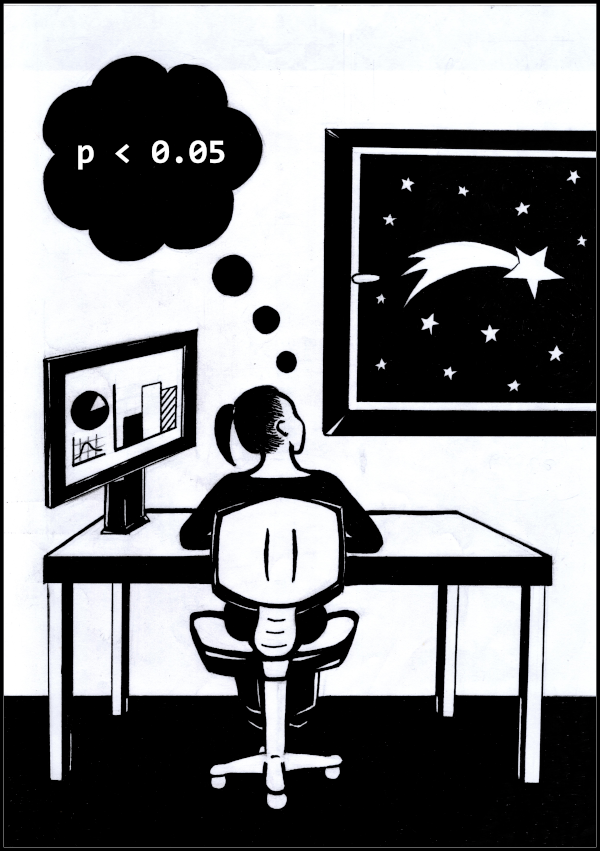
\includegraphics[width=0.7\linewidth]{images/ch_10_small} \end{center}

\begin{rmdlevel1}
Ebben a fejezetben a statisztika azon klasszikus próbáit foglaltuk össze, amelyek jellemzően egy- vagy kétmintás hipotézisvizsgálatokat jelentenek. Az öt alfejezet a nullhipotézisben szereplő állításoknak és paramétereknek megfelelően a statisztikai próbák különböző csoportjait fedi le:

\begin{itemize}
\tightlist
\item
  várható értékre vonatkozó próbák
\item
  mediánra vonatkozó nemparaméteres próbák
\item
  valószínűségre vonatkozó próbák
\item
  varianciára vonatkozó próbák
\item
  az eloszlás egészére vonatkozó próbák.
\end{itemize}
\end{rmdlevel1}

\hypertarget{hipotuxe9zisvizsguxe1latok}{%
\section{Hipotézisvizsgálatok}\label{hipotuxe9zisvizsguxe1latok}}

\hypertarget{tidyverse-r}{%
\section{Tidyverse R}\label{tidyverse-r}}

\hypertarget{haladuxf3-lehetux151suxe9gek-1}{%
\section{Haladó lehetőségek}\label{haladuxf3-lehetux151suxe9gek-1}}

A fejezetben bemutatott hipotézisvizsgáló függvények közös tulajdonságait három megjegyzésben foglaltuk össze.

\begin{itemize}
\tightlist
\item
  \textbf{1. megjegyzés: konfidencia-intervallum kiszámítása a hipotézisvizsgálat során}
\end{itemize}

A hipotézisvizsgáló függvények outputjában sok esetben konfidencia-intervallum is megjelenik. Ezekben a függvényekben a \texttt{conf.level=} argumentum segítségével szabályozhatjuk a megbízhatósági szintet. Alapértelmezés szerint a függvények \texttt{conf.level=0.95} argumentummal hívódnak, azaz a 95\%-os konfidencia-intervallum határai jelennek meg az outputokban. Az argumentum értékét megváltoztathatjuk, így tetszőleges megbízhatósági szintű intervallumbecslésre van módunk. Mindezt a \texttt{t.test()} segítségével mutatjuk be. Ha nem adjuk meg híváskor a \texttt{conf.level=} argumentumot, akkor 95\%-os lesz az intervallumbecslés megbízhatósága.

\begin{Shaded}
\begin{Highlighting}[]
\CommentTok{\# a konfidencia{-}intervallum alapértelmezett (95\%{-}os) megbízhatósággal}
\NormalTok{x }\OtherTok{\textless{}{-}} \FunctionTok{c}\NormalTok{(}\DecValTok{9}\NormalTok{, }\DecValTok{10}\NormalTok{, }\DecValTok{6}\NormalTok{, }\DecValTok{4}\NormalTok{, }\DecValTok{8}\NormalTok{, }\DecValTok{11}\NormalTok{, }\DecValTok{10}\NormalTok{, }\DecValTok{5}\NormalTok{, }\DecValTok{5}\NormalTok{, }\DecValTok{6}\NormalTok{, }\DecValTok{13}\NormalTok{, }\DecValTok{12}\NormalTok{)}
\FunctionTok{t.test}\NormalTok{(x, }\AttributeTok{mu=}\DecValTok{8}\NormalTok{)  }
\CommentTok{\#\textgreater{} }
\CommentTok{\#\textgreater{}  One Sample t{-}test}
\CommentTok{\#\textgreater{} }
\CommentTok{\#\textgreater{} data:  x}
\CommentTok{\#\textgreater{} t = 0.29, df = 11, p{-}value = 0.8}
\CommentTok{\#\textgreater{} alternative hypothesis: true mean is not equal to 8}
\CommentTok{\#\textgreater{} 95 percent confidence interval:}
\CommentTok{\#\textgreater{}   6.332 10.168}
\CommentTok{\#\textgreater{} sample estimates:}
\CommentTok{\#\textgreater{} mean of x }
\CommentTok{\#\textgreater{}      8.25}
\end{Highlighting}
\end{Shaded}

Ha 99\%-os megbízhatóságú konfidencia-intervallumot szeretnénk meghatározni, akkor a \texttt{conf.level=0.99} argumentumot kell használni. Figyeljük meg, hogy a \texttt{conf.level=} argumentum kizárólag az intervallum határait befolyásolja, más mutatók nem változnak az outputban.

\begin{Shaded}
\begin{Highlighting}[]
\CommentTok{\# a konfidencia{-}intervallum 99\%{-}os megbízhatósággal}
\NormalTok{x }\OtherTok{\textless{}{-}} \FunctionTok{c}\NormalTok{(}\DecValTok{9}\NormalTok{, }\DecValTok{10}\NormalTok{, }\DecValTok{6}\NormalTok{, }\DecValTok{4}\NormalTok{, }\DecValTok{8}\NormalTok{, }\DecValTok{11}\NormalTok{, }\DecValTok{10}\NormalTok{, }\DecValTok{5}\NormalTok{, }\DecValTok{5}\NormalTok{, }\DecValTok{6}\NormalTok{, }\DecValTok{13}\NormalTok{, }\DecValTok{12}\NormalTok{)}
\FunctionTok{t.test}\NormalTok{(x, }\AttributeTok{mu=}\DecValTok{8}\NormalTok{, }\AttributeTok{conf.level=}\FloatTok{0.99}\NormalTok{)  }
\CommentTok{\#\textgreater{} }
\CommentTok{\#\textgreater{}  One Sample t{-}test}
\CommentTok{\#\textgreater{} }
\CommentTok{\#\textgreater{} data:  x}
\CommentTok{\#\textgreater{} t = 0.29, df = 11, p{-}value = 0.8}
\CommentTok{\#\textgreater{} alternative hypothesis: true mean is not equal to 8}
\CommentTok{\#\textgreater{} 99 percent confidence interval:}
\CommentTok{\#\textgreater{}   5.543 10.957}
\CommentTok{\#\textgreater{} sample estimates:}
\CommentTok{\#\textgreater{} mean of x }
\CommentTok{\#\textgreater{}      8.25}
\end{Highlighting}
\end{Shaded}

\begin{itemize}
\tightlist
\item
  \textbf{2. megjegyzés: kétoldali és egyoldali próbák}
\end{itemize}

A hipotézisvizsgáló függvények hívása során az \texttt{alternative=} argumentummal határozzuk meg, hogy kétoldali vagy egyoldali (bal- vagy jobb-oldali) próbát szeretnénk végrehajtani. Az alapértelmezés a kétoldali próba, amely az \texttt{alternative="two.sided"} hívásnak felel meg. Az \texttt{alternative=} argumentum lehetséges értéke még a \texttt{"less"} és a \texttt{"greater"}.

Összefoglaltuk az \texttt{alternative=} argumentum lehetséges értékei és a próbák null- és ellenhipotézisei közötti összefüggést egy- és kétmintás esetben:

\begin{itemize}
\item
  Egymintás próbák
\item
  \texttt{alternative="two.sided"} (kétoldali próba)\\
  \(H_0:\mu=\mu_0\)\\
  \(H_1:\mu\neq\mu_0\)
\item
  \texttt{alternative="less"} (bal-oldali próba)\\
  \(H_0:\mu=\mu_0\)\\
  \(H_1:\mu < \mu_0\)
\item
  \texttt{alternative="greater"} (jobb-oldali próba)\\
  \(H_0:\mu=\mu_0\)\\
  \(H_1:\mu > \mu_0\)
\item
  Kétmintás próbák
\item
  \texttt{alternative="two.sided"} (kétoldali próba)\\
  \(H_0:\mu_1=\mu_2\) (vagy \(H_0:\mu_1-\mu_2=0\))\\
  \(H_1:\mu_1\neq\mu_2\) (vagy \(H_1:\mu_1-\mu_2 \neq 0\))\\
\item
  \texttt{alternative="less"} (bal-oldali próba)\\
  \(H_0:\mu_1=\mu_2\) (vagy \(H_0:\mu_1-\mu_2=0\))\\
  \(H_1:\mu_1 < \mu_2\) (vagy \(H_1:\mu_1-\mu_2 < 0\))
\item
  \texttt{alternative="greater"} (jobb-oldali próba)\\
  \(H_0:\mu_1=\mu_2\) (vagy \(H_0:\mu_1\mu_2=0\))\\
  \(H_1:\mu_1 > \mu_2\) (vagy \(H_1:\mu_1-\mu_2 > 0\))
\item
  \textbf{3. megjegyzés: a hipotézisvizsgáló függvények visszatérési értéke}
\end{itemize}

Mielőtt a próbák végrehajtását részletezni kezdjük érdemes még megjegyezni, hogy a hipotézisvizsgáló függvények kétféle módon is használhatók:

\begin{itemize}
\tightlist
\item
  Az első használati mód szerint a függvényt a megfelelő paraméterekkel meghívjuk és a konzolban megjelenő eredményt értelmezzük. Erre látunk példát fentebb.
\item
  A másik eset azon alapul, hogy a fenti egyszerűbb használaton túlhaladva, közvetlenül is hozzá szeretnénk férni a hipotézisvizsgálat eredményében leolvasható mutatókhoz, vagy azokhoz az adatokhoz, amelyek meg sem jelennek a próba outputjában. Ezek szemléltetésére az egymintás t-próbát megvalósító \texttt{t.test()} függvényt hívjuk segítségül, de természetesen bármely másik hipotézisvizsgáló függvényt is választhattuk volna.
\end{itemize}

Tekintsük az első, egyszerűbb esetet, amikor a próba végrehajtásra mindössze a próba eredményének a képernyőre írását jelenti.

\begin{Shaded}
\begin{Highlighting}[]
\CommentTok{\# 1. használati mód: a próba eredménye a képernyőre kerül}
\NormalTok{x }\OtherTok{\textless{}{-}} \FunctionTok{c}\NormalTok{(}\DecValTok{9}\NormalTok{, }\DecValTok{10}\NormalTok{, }\DecValTok{6}\NormalTok{, }\DecValTok{4}\NormalTok{, }\DecValTok{8}\NormalTok{, }\DecValTok{11}\NormalTok{, }\DecValTok{10}\NormalTok{, }\DecValTok{5}\NormalTok{, }\DecValTok{5}\NormalTok{, }\DecValTok{6}\NormalTok{, }\DecValTok{13}\NormalTok{, }\DecValTok{12}\NormalTok{)}
\FunctionTok{t.test}\NormalTok{(x, }\AttributeTok{mu=}\DecValTok{8}\NormalTok{)  }
\CommentTok{\#\textgreater{} }
\CommentTok{\#\textgreater{}  One Sample t{-}test}
\CommentTok{\#\textgreater{} }
\CommentTok{\#\textgreater{} data:  x}
\CommentTok{\#\textgreater{} t = 0.29, df = 11, p{-}value = 0.8}
\CommentTok{\#\textgreater{} alternative hypothesis: true mean is not equal to 8}
\CommentTok{\#\textgreater{} 95 percent confidence interval:}
\CommentTok{\#\textgreater{}   6.332 10.168}
\CommentTok{\#\textgreater{} sample estimates:}
\CommentTok{\#\textgreater{} mean of x }
\CommentTok{\#\textgreater{}      8.25}
\end{Highlighting}
\end{Shaded}

A hipotézisvizsgálat eredménye ugyan a fenti leolvasható, de sokszor van szükségünk a képernyőn megjelenő adatok közvetlen elérésére, vagy azokra az adatokra, amelyeket a hipotézisvizsgáló függvények kiszámolnak, de alapértelmezetten nem jelenítenek meg. A \texttt{t.test()} függvény visszatérési értékét ezért most elmentjük egy \texttt{h.data} adatobjektumban, amelyet később fel fogunk használni. Az első esetnek megfelelő szokásos megjelenítést a \texttt{h.data} adatobjektum nevének parancssorba írásával érhetjük el:

\begin{Shaded}
\begin{Highlighting}[]
\CommentTok{\# 2. használati mód: t{-}próba végrehajtása és a visszatérési érték elmentése egy adatobjektumban}
\NormalTok{x }\OtherTok{\textless{}{-}} \FunctionTok{c}\NormalTok{(}\DecValTok{9}\NormalTok{, }\DecValTok{10}\NormalTok{, }\DecValTok{6}\NormalTok{, }\DecValTok{4}\NormalTok{, }\DecValTok{8}\NormalTok{, }\DecValTok{11}\NormalTok{, }\DecValTok{10}\NormalTok{, }\DecValTok{5}\NormalTok{, }\DecValTok{5}\NormalTok{, }\DecValTok{6}\NormalTok{, }\DecValTok{13}\NormalTok{, }\DecValTok{12}\NormalTok{)}
\NormalTok{h.data }\OtherTok{\textless{}{-}} \FunctionTok{t.test}\NormalTok{(x, }\AttributeTok{mu=}\DecValTok{8}\NormalTok{)  }
\NormalTok{h.data }\CommentTok{\# a próba eredményének megjelenítése}
\CommentTok{\#\textgreater{} }
\CommentTok{\#\textgreater{}  One Sample t{-}test}
\CommentTok{\#\textgreater{} }
\CommentTok{\#\textgreater{} data:  x}
\CommentTok{\#\textgreater{} t = 0.29, df = 11, p{-}value = 0.8}
\CommentTok{\#\textgreater{} alternative hypothesis: true mean is not equal to 8}
\CommentTok{\#\textgreater{} 95 percent confidence interval:}
\CommentTok{\#\textgreater{}   6.332 10.168}
\CommentTok{\#\textgreater{} sample estimates:}
\CommentTok{\#\textgreater{} mean of x }
\CommentTok{\#\textgreater{}      8.25}
\end{Highlighting}
\end{Shaded}

Egyelőre az outputban visszakaptuk a próba eredményét a képernyőn a második használati mód mellett is. A fenti parancsoknak azonban az az előnye, hogy rendelkezésre áll a \texttt{h.data} objektum, amely a hipotézisvizsgálat során kiszámolt adatelemeket tárolja. Az adatelemeket felhasználhatjuk a későbbi parancsainkban, például újabb, eddig nem tárolt mérőszámok meghatározásához, vagy ábrák létrehozásához. A példánknál maradva a \texttt{t.test()} függvény a hívása során kiszámolja a konfidencia-intervallum határait, amelyet a \texttt{h.data} adatobjektum \texttt{\$conf.int} eleme tartalmaz. Ezt többféle módon is felhasználhatjuk. Egyszerűen a képernyőre írathatjuk az intervallum határait, de az intervallum hosszát is meghatározhatjuk a \texttt{diff()} függvény segítségével.

\begin{Shaded}
\begin{Highlighting}[]
\CommentTok{\# a 95\%{-}os megbízhatóságú konfidencia{-}intervallum }
\NormalTok{h.data}\SpecialCharTok{$}\NormalTok{conf.int}
\CommentTok{\#\textgreater{} [1]  6.332 10.168}
\CommentTok{\#\textgreater{} attr(,"conf.level")}
\CommentTok{\#\textgreater{} [1] 0.95}
\end{Highlighting}
\end{Shaded}

\begin{Shaded}
\begin{Highlighting}[]
\CommentTok{\# a 95\%{-}os megbízhatóságú konfidencia{-}intervallum hossza}
\FunctionTok{diff}\NormalTok{(h.data}\SpecialCharTok{$}\NormalTok{conf.int)}
\CommentTok{\#\textgreater{} [1] 3.836}
\end{Highlighting}
\end{Shaded}

A statisztikai próba típusa meghatározza, hogy a \texttt{h.data} adatobjektumon belül, milyen adatelemek érhetők el. Ezek eltérhetnek egymástól, hiszen más számítás tartozik például egy t-próbához és más egy khi-négyzet próbához. Ha kíváncsiak vagyunk az elérhető adatelemekre, akkor a \texttt{names()} függvénnyel az adatelemek nevét, az \texttt{unclass()} függvénnyel a neveken túl az adatelemek értékét is megjeleníthetjük output).

\begin{Shaded}
\begin{Highlighting}[]
\FunctionTok{names}\NormalTok{(h.data) }\CommentTok{\# a h.data lista elemeinek neve}
\CommentTok{\#\textgreater{}  [1] "statistic"   "parameter"   "p.value"     "conf.int"    "estimate"   }
\CommentTok{\#\textgreater{}  [6] "null.value"  "stderr"      "alternative" "method"      "data.name"}
\FunctionTok{unclass}\NormalTok{(h.data) }\CommentTok{\# a h.data lista elemeinek neve és értéke}
\CommentTok{\#\textgreater{} $statistic}
\CommentTok{\#\textgreater{}      t }
\CommentTok{\#\textgreater{} 0.2869 }
\CommentTok{\#\textgreater{} }
\CommentTok{\#\textgreater{} $parameter}
\CommentTok{\#\textgreater{} df }
\CommentTok{\#\textgreater{} 11 }
\CommentTok{\#\textgreater{} }
\CommentTok{\#\textgreater{} $p.value}
\CommentTok{\#\textgreater{} [1] 0.7795}
\CommentTok{\#\textgreater{} }
\CommentTok{\#\textgreater{} $conf.int}
\CommentTok{\#\textgreater{} [1]  6.332 10.168}
\CommentTok{\#\textgreater{} attr(,"conf.level")}
\CommentTok{\#\textgreater{} [1] 0.95}
\CommentTok{\#\textgreater{} }
\CommentTok{\#\textgreater{} $estimate}
\CommentTok{\#\textgreater{} mean of x }
\CommentTok{\#\textgreater{}      8.25 }
\CommentTok{\#\textgreater{} }
\CommentTok{\#\textgreater{} $null.value}
\CommentTok{\#\textgreater{} mean }
\CommentTok{\#\textgreater{}    8 }
\CommentTok{\#\textgreater{} }
\CommentTok{\#\textgreater{} $stderr}
\CommentTok{\#\textgreater{} [1] 0.8715}
\CommentTok{\#\textgreater{} }
\CommentTok{\#\textgreater{} $alternative}
\CommentTok{\#\textgreater{} [1] "two.sided"}
\CommentTok{\#\textgreater{} }
\CommentTok{\#\textgreater{} $method}
\CommentTok{\#\textgreater{} [1] "One Sample t{-}test"}
\CommentTok{\#\textgreater{} }
\CommentTok{\#\textgreater{} $data.name}
\CommentTok{\#\textgreater{} [1] "x"}
\end{Highlighting}
\end{Shaded}

\begin{Shaded}
\begin{Highlighting}[]
\FunctionTok{unclass}\NormalTok{(h.data) }\CommentTok{\# a h.data lista elemeinek neve és értéke}
\CommentTok{\#\textgreater{} $statistic}
\CommentTok{\#\textgreater{}      t }
\CommentTok{\#\textgreater{} 0.2869 }
\CommentTok{\#\textgreater{} }
\CommentTok{\#\textgreater{} $parameter}
\CommentTok{\#\textgreater{} df }
\CommentTok{\#\textgreater{} 11 }
\CommentTok{\#\textgreater{} }
\CommentTok{\#\textgreater{} $p.value}
\CommentTok{\#\textgreater{} [1] 0.7795}
\CommentTok{\#\textgreater{} }
\CommentTok{\#\textgreater{} $conf.int}
\CommentTok{\#\textgreater{} [1]  6.332 10.168}
\CommentTok{\#\textgreater{} attr(,"conf.level")}
\CommentTok{\#\textgreater{} [1] 0.95}
\CommentTok{\#\textgreater{} }
\CommentTok{\#\textgreater{} $estimate}
\CommentTok{\#\textgreater{} mean of x }
\CommentTok{\#\textgreater{}      8.25 }
\CommentTok{\#\textgreater{} }
\CommentTok{\#\textgreater{} $null.value}
\CommentTok{\#\textgreater{} mean }
\CommentTok{\#\textgreater{}    8 }
\CommentTok{\#\textgreater{} }
\CommentTok{\#\textgreater{} $stderr}
\CommentTok{\#\textgreater{} [1] 0.8715}
\CommentTok{\#\textgreater{} }
\CommentTok{\#\textgreater{} $alternative}
\CommentTok{\#\textgreater{} [1] "two.sided"}
\CommentTok{\#\textgreater{} }
\CommentTok{\#\textgreater{} $method}
\CommentTok{\#\textgreater{} [1] "One Sample t{-}test"}
\CommentTok{\#\textgreater{} }
\CommentTok{\#\textgreater{} $data.name}
\CommentTok{\#\textgreater{} [1] "x"}
\end{Highlighting}
\end{Shaded}

A fenti outputokból leolvasható, hogy összesen 9 db adatelem áll rendelkezésre a \texttt{h.data} adatobjektumban. Ezek egy része szöveges, és a t-próba megfogalmazásáért felelős (\texttt{\$method}, \texttt{\$alternative}, \texttt{\$data.name}), míg más adatelemek a kiszámolt mutatókat tartalmazzák, például a próbastatisztika értékét (\texttt{\$statistic}) vagy a p értéket (\texttt{\$p.value}).

A kétféle használati mód közül az alapján választhatunk, hogy az adott szituációban mire van szükségünk. Ha a próba képernyőn megjelenő eredménye elegendő a feladat megoldásához, akkor az első esetet választjuk. Ha azonban további műveleteket szeretnénk végrehajtani az eredmény egyes elemeivel, akkor tanácsos a második módszer mellett dönteni.

\hypertarget{pruxf3buxe1k-vuxe1lasztuxe1sa}{%
\section{Próbák választása}\label{pruxf3buxe1k-vuxe1lasztuxe1sa}}

Egymintás előjel-próba

\hypertarget{pruxf3buxe1k-kuxf6zuxe9puxe9rtuxe9kekre}{%
\section{Próbák középértékekre}\label{pruxf3buxe1k-kuxf6zuxe9puxe9rtuxe9kekre}}

A statisztika tanulmányozása során elsajátított első próbák intervallum vagy arány skálán mért változókat hasonlítanak össze egymással vagy egy meghatározott értékkel. Ezek közé tartoznak az u-próba és a t-próba különböző változatai. Ebben a fejezetben a \texttt{BSDA::z.test()} és a \texttt{t.test()} függvényt ismertetjük részletesen. Mindkét függvény használható egymintás, kétmintás és páros mintás esetben is. A \texttt{BSDA::z.test()} fügvénnyel az u-próba, míg a \texttt{t.test()} függvénnyel a t-próba különböző változatait hajthatjuk végre. A \texttt{z.test()} függvényt a \texttt{BSDA} és a \texttt{TeachingDemos} csomagban is megvalósították, mindkettőről ejtünk szót.

Adatbázis nélkül is elvégezhetjük a fenti hipotézisvizsgálatokat a \texttt{BSDA} csomag \texttt{zsum.test()} és \texttt{tsum.test()} függvényeinek segítségével. Elegendő a mintaátlag, a mintaelemszám és esetleg a minta szórásának megadása az argumentumokban. Ezen függvények működését is bemutatjuk.

A következő öt alfejezet a várható értékre vonatkozó egy- és kétmintás próbákat tartalmazza:

\begin{figure}
\centering
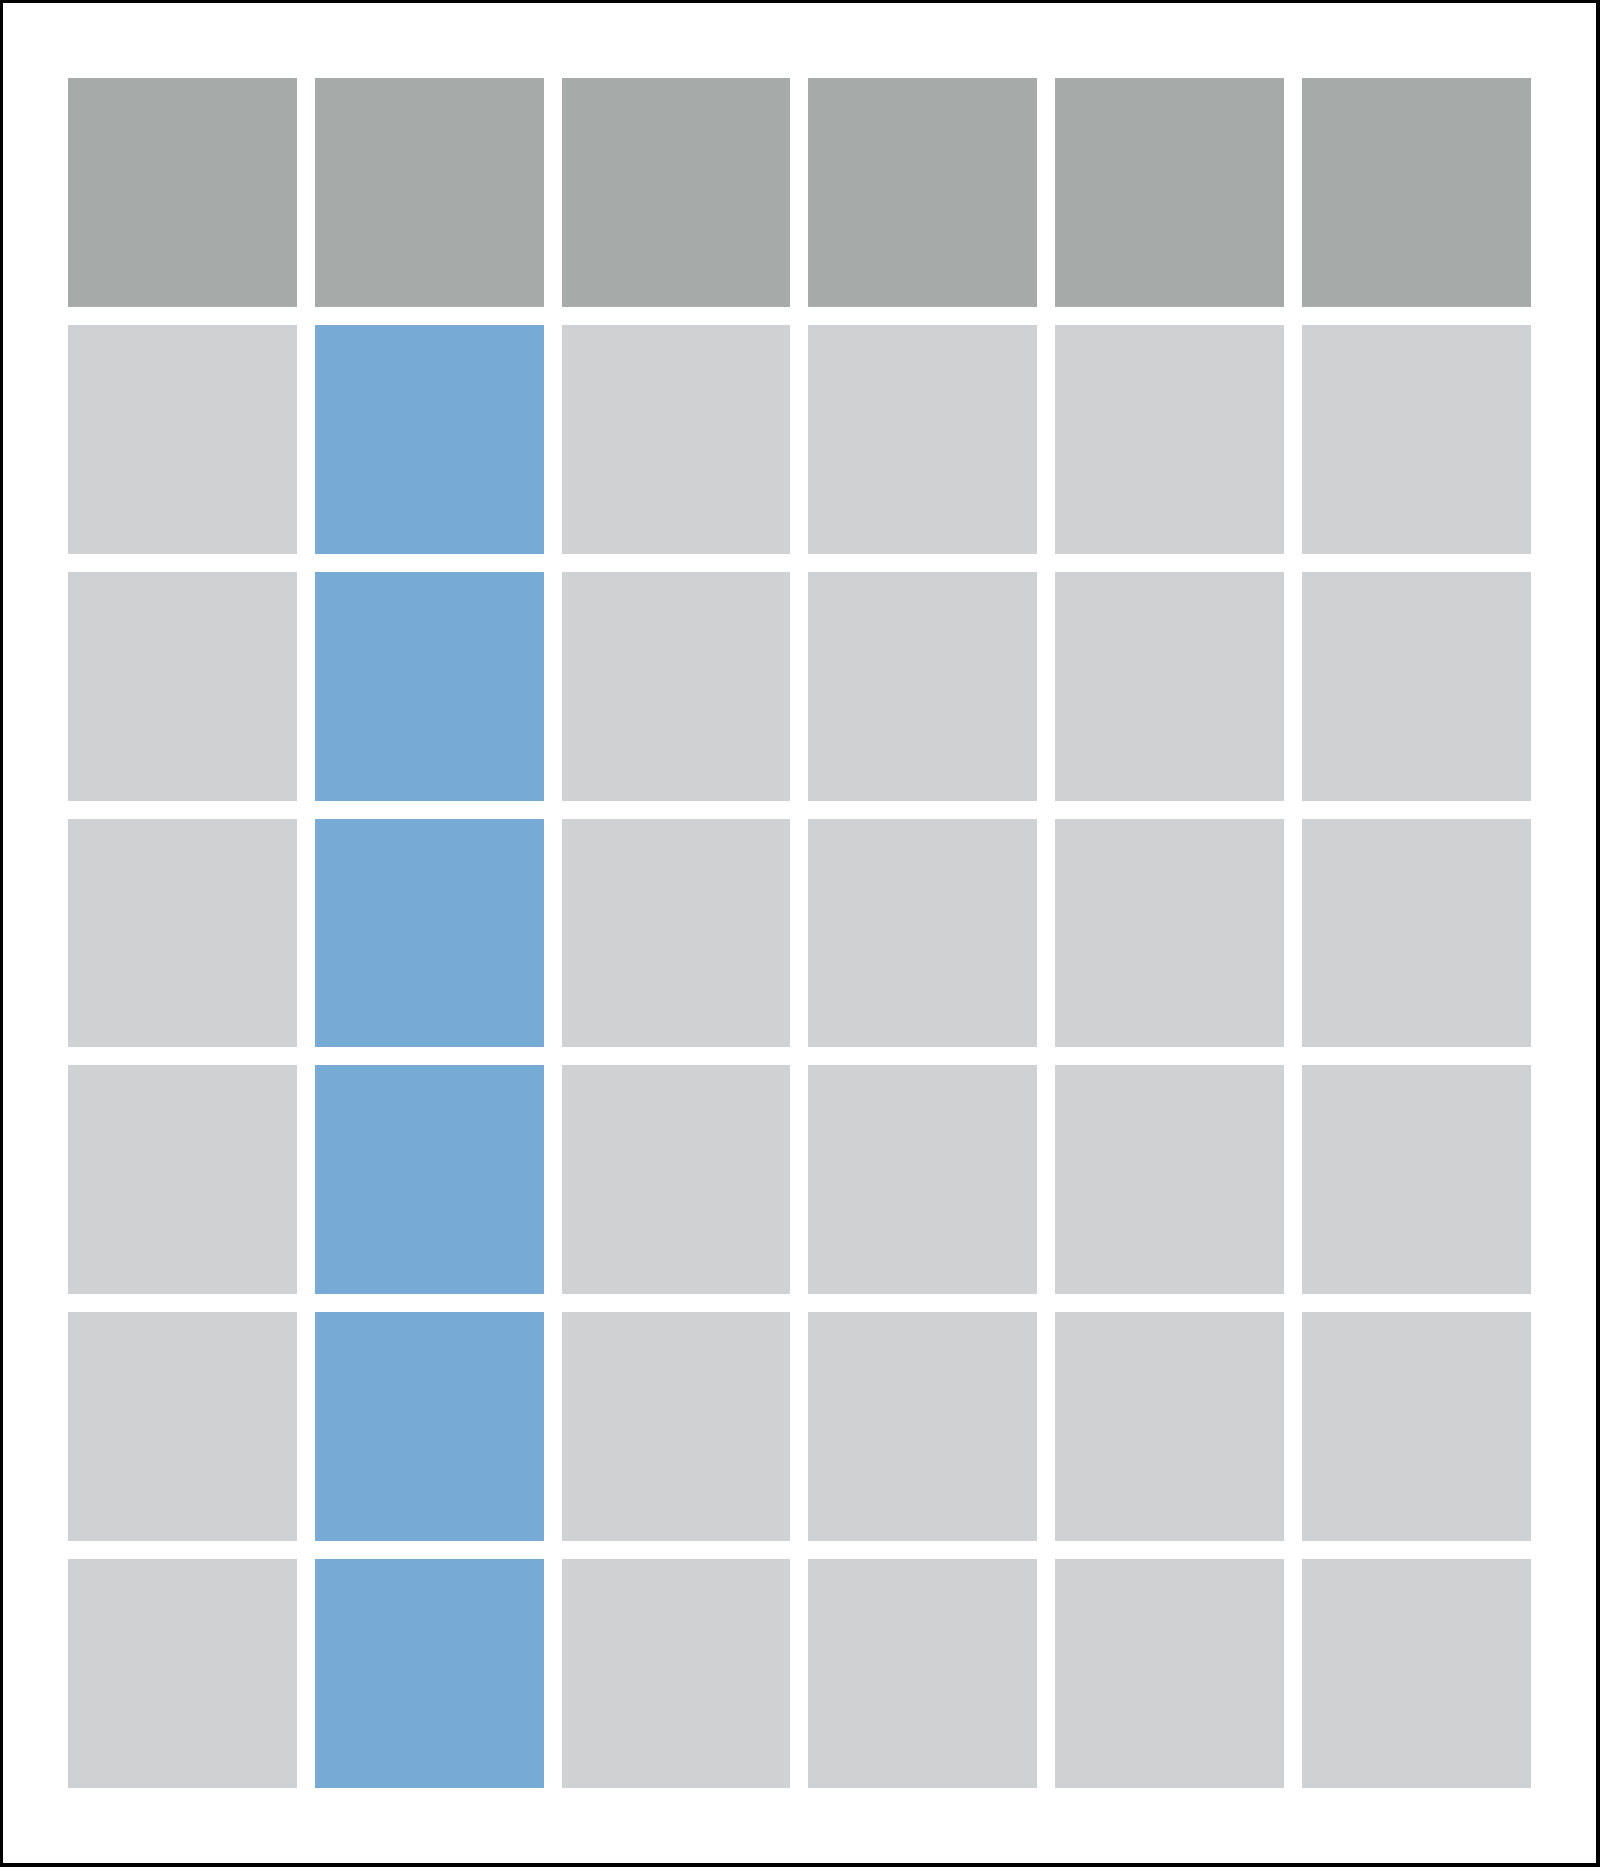
\includegraphics{images_df/df_egymintas.png}
\caption{Egymintás próbák adatszerkezete}
\end{figure}

\begin{longtable}[]{@{}
  >{\raggedright\arraybackslash}p{(\columnwidth - 2\tabcolsep) * \real{0.6458}}
  >{\raggedright\arraybackslash}p{(\columnwidth - 2\tabcolsep) * \real{0.3542}}@{}}
\toprule
\begin{minipage}[b]{\linewidth}\raggedright
Egymintás próba neve
\end{minipage} & \begin{minipage}[b]{\linewidth}\raggedright
R függvény
\end{minipage} \\
\midrule
\endhead
egymintás u-próba & \texttt{PASWR2::z.test(x,\ sigma.x,\ mu)} \\
egymintás t-próba & \texttt{t.test(x,\ mu)} \\
előjel-próba & \texttt{DescTools::SignTest()} \\
egymintás Wilcoxon-próba & \texttt{wilcox.test(x,\ mu)} \\
Mood-féle medián-próba & \texttt{fisher.test(x,\ y)} \texttt{chisq.test(x,\ y)} \\
\bottomrule
\end{longtable}

\begin{figure}
\centering
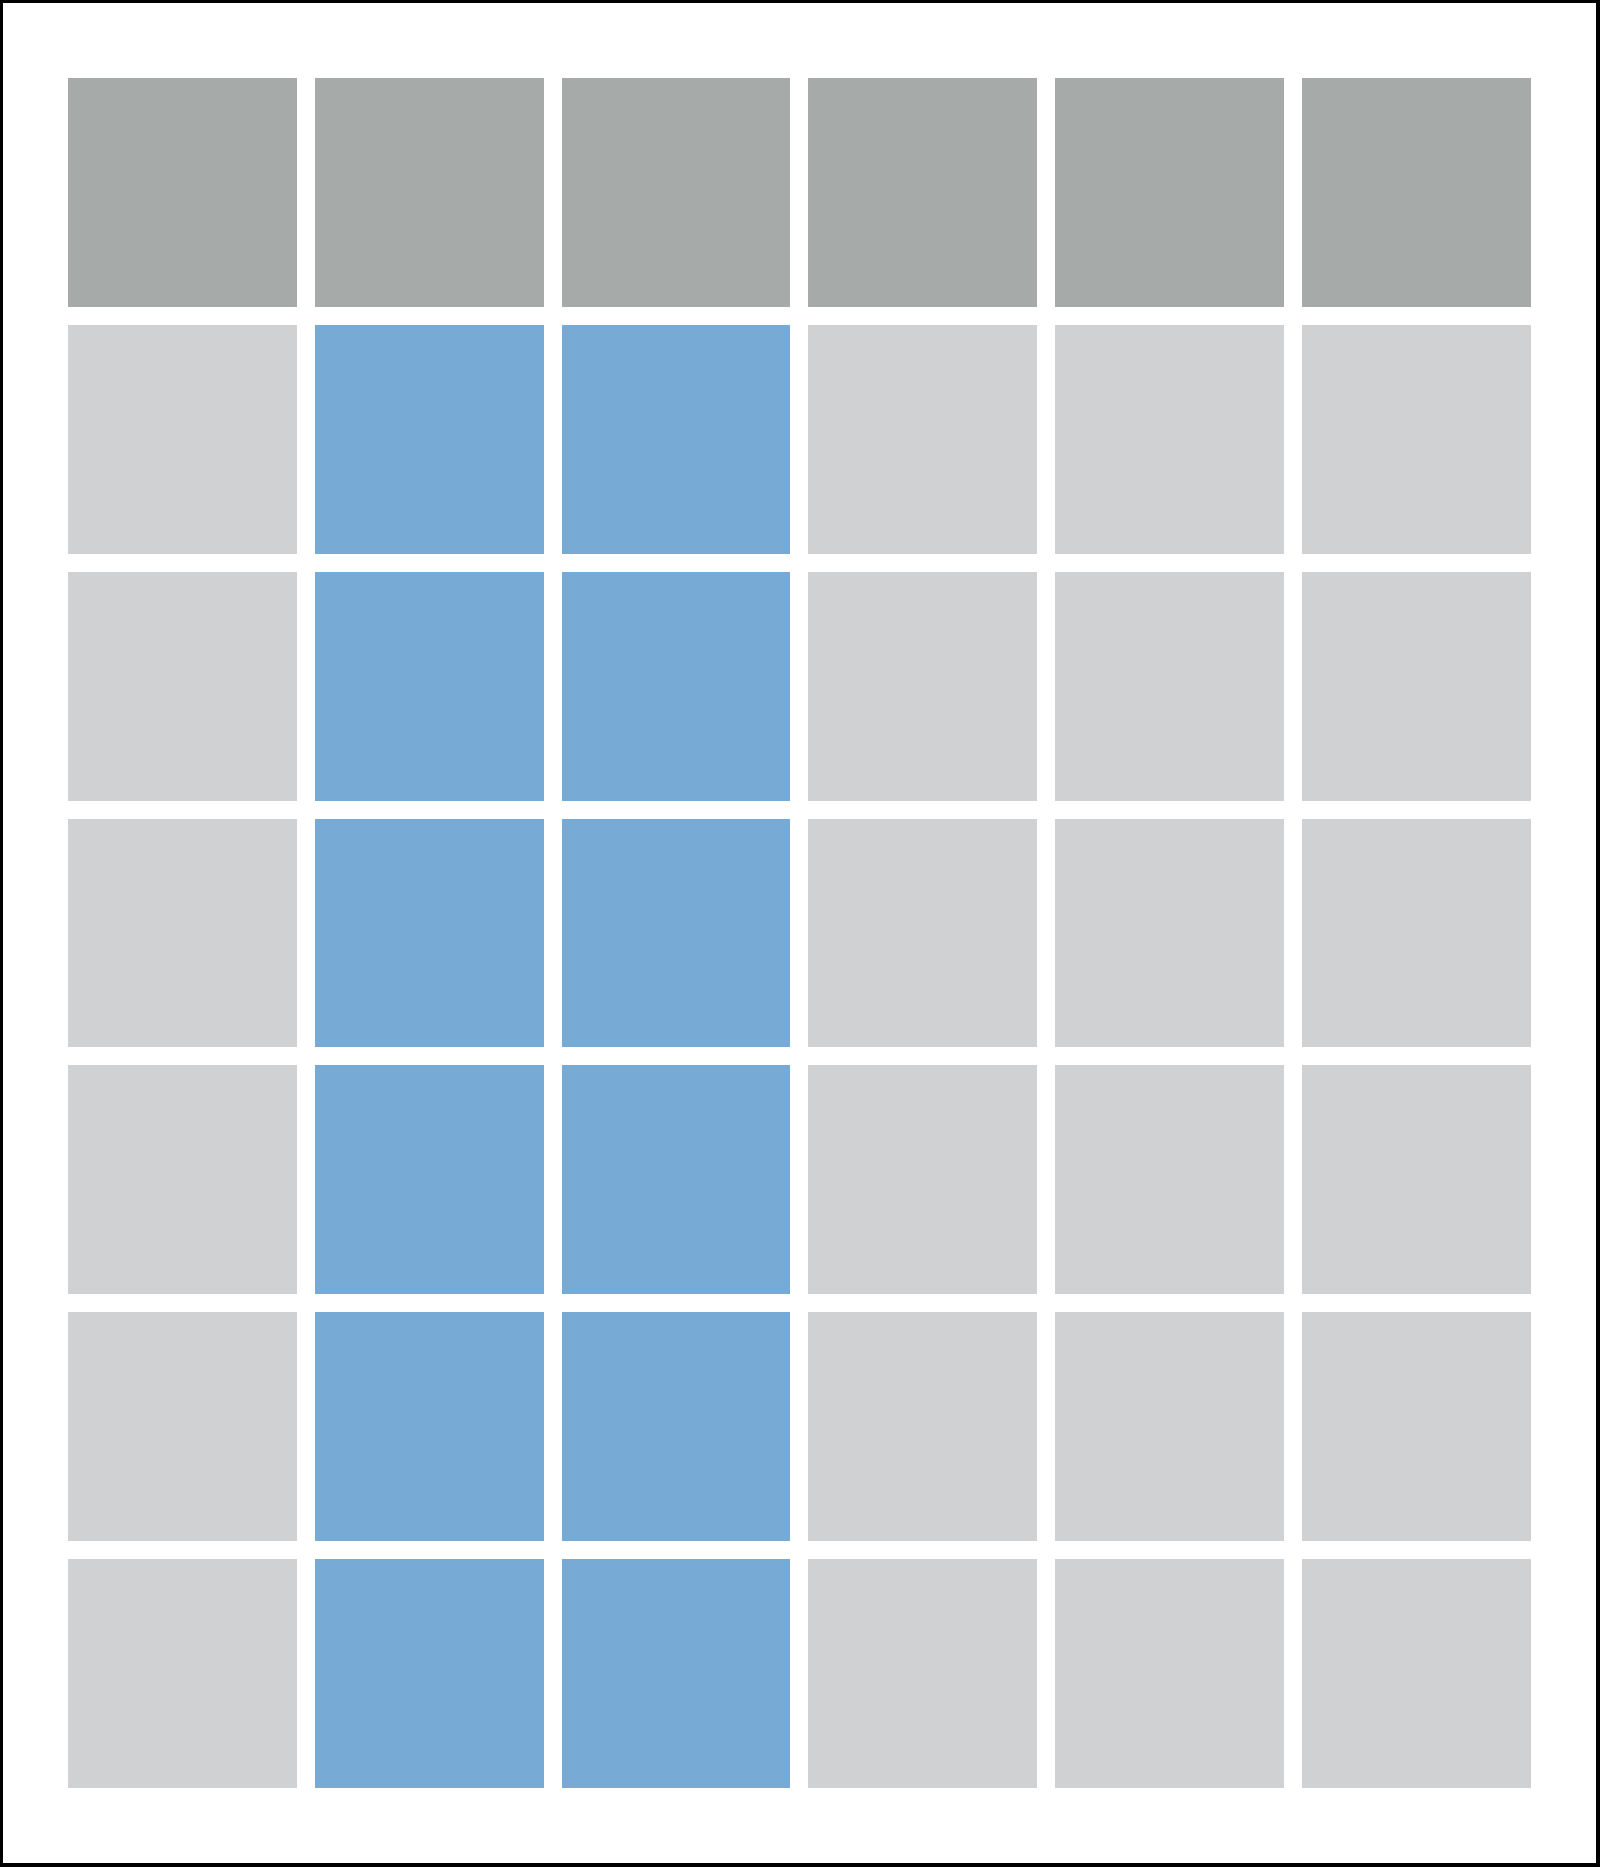
\includegraphics{images_df/df_parosmintas.png}
\caption{Páros próbák adatszerkezete}
\end{figure}

\begin{longtable}[]{@{}ll@{}}
\toprule
Páros próba neve & R függvény \\
\midrule
\endhead
páros u-próba & \texttt{PASWR2::z.test(x,\ y,\ paired=T)} \\
páros t-próba & \texttt{t.test(x,\ y,\ paired=T)} \\
páros Wilcoxon-próba & \texttt{wilcox.test(x,\ y,\ paired=T)} \\
páros előjel-próba & \texttt{DescTools::SignTest()} \\
\bottomrule
\end{longtable}

\begin{figure}
\centering
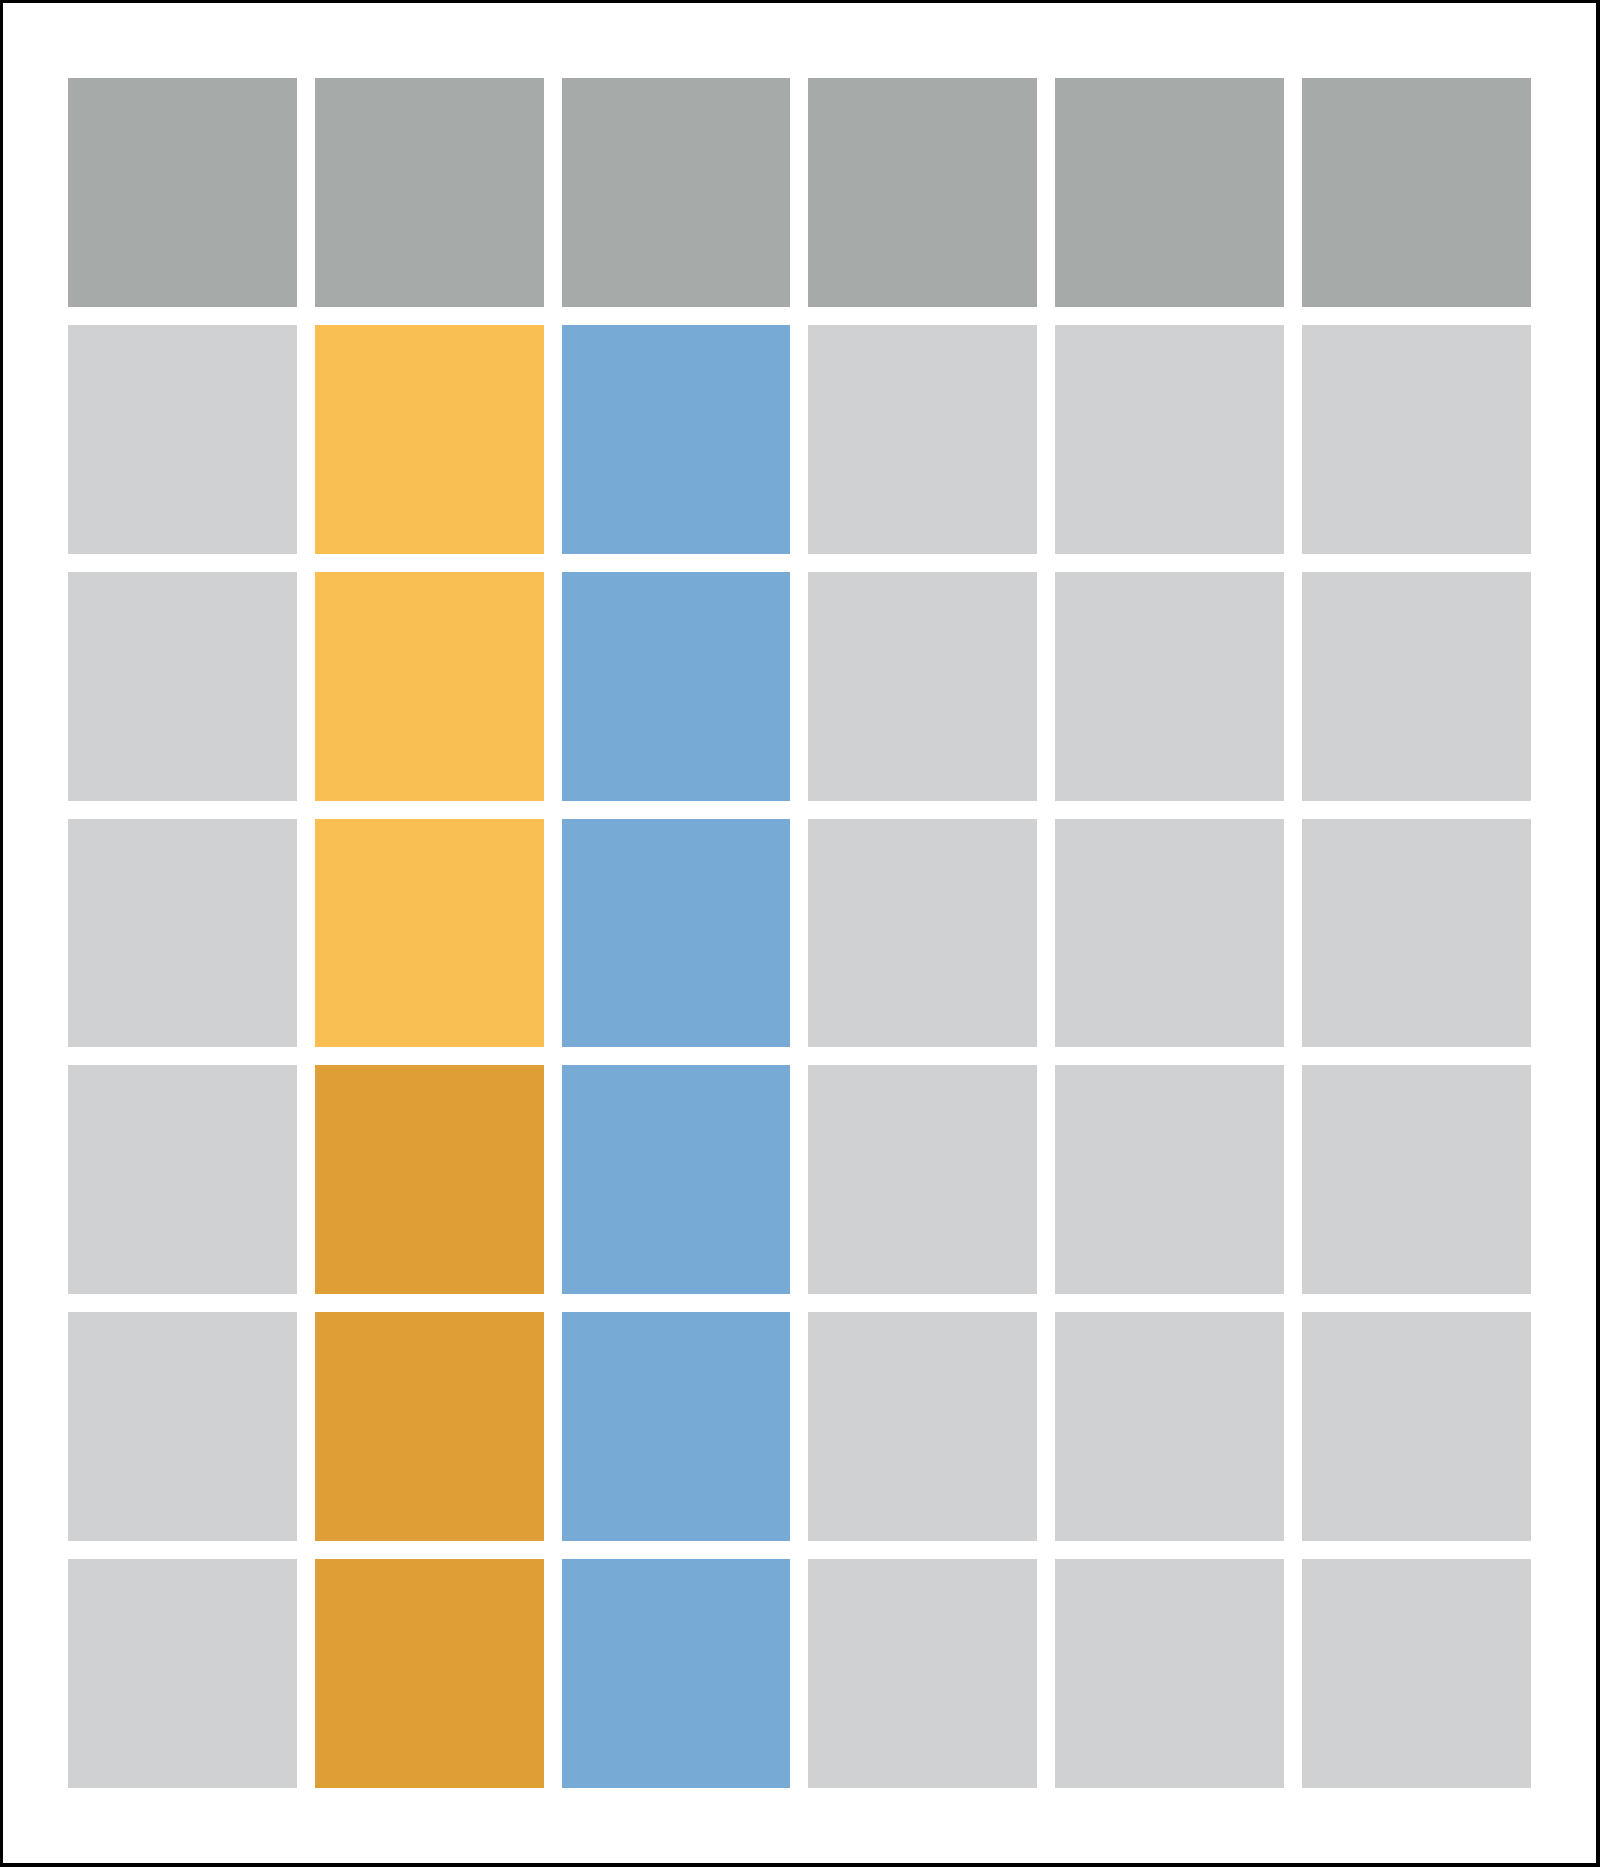
\includegraphics{images_df/df_ketmintas.png}
\caption{Kétmintás próbák adatszerkezete}
\end{figure}

\begin{longtable}[]{@{}
  >{\raggedright\arraybackslash}p{(\columnwidth - 2\tabcolsep) * \real{0.6458}}
  >{\raggedright\arraybackslash}p{(\columnwidth - 2\tabcolsep) * \real{0.3542}}@{}}
\toprule
\begin{minipage}[b]{\linewidth}\raggedright
Kétmintás próba neve
\end{minipage} & \begin{minipage}[b]{\linewidth}\raggedright
R függvény
\end{minipage} \\
\midrule
\endhead
kétmintás u-próba & \texttt{PASWR2::z.test(x,\ y,\ sigma.x,\ sigma.y)} \\
kétmintás t-próba & \texttt{t.test(x,\ y)} \texttt{t.test(formula,\ data)} \\
Welch-féle d-próba & \texttt{t.test(x,\ y,\ )} \texttt{t.test(formula,\ data)} \\
Mann--Whitney-féle U-próba & \texttt{wilcox.test(x,y)} \texttt{wilcox.test(formula,\ data)} \\
\bottomrule
\end{longtable}

\begin{figure}
\centering
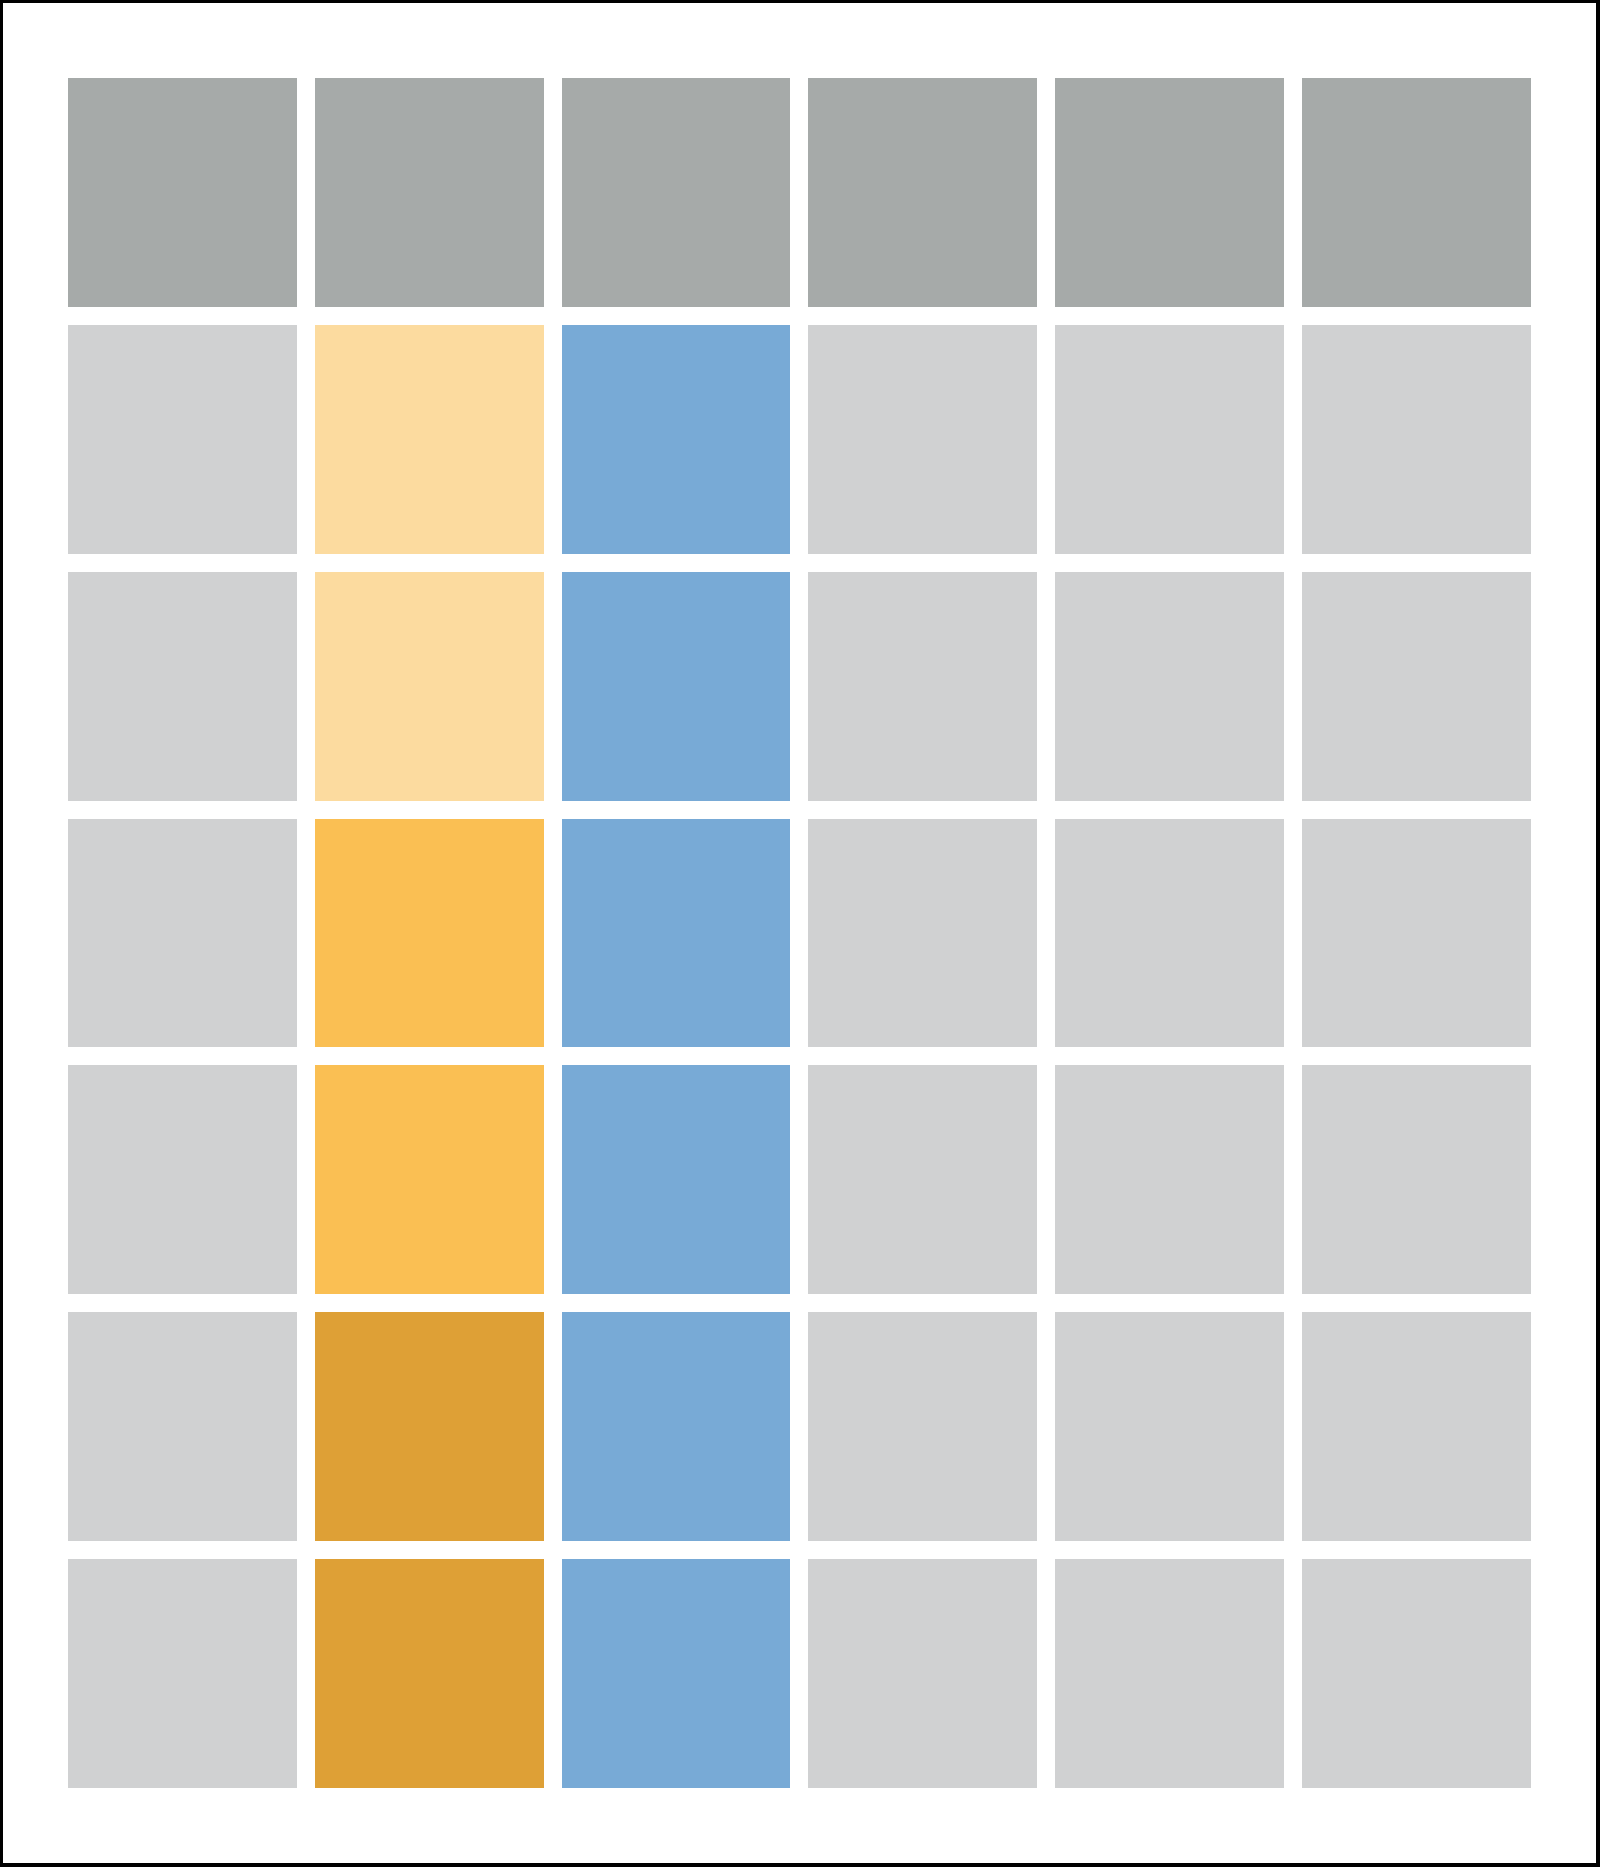
\includegraphics{images_df/df_tobbmintas.png}
\caption{Többmintás próbák adatszerkezete}
\end{figure}

\begin{longtable}[]{@{}
  >{\raggedright\arraybackslash}p{(\columnwidth - 2\tabcolsep) * \real{0.6458}}
  >{\raggedright\arraybackslash}p{(\columnwidth - 2\tabcolsep) * \real{0.3542}}@{}}
\toprule
\begin{minipage}[b]{\linewidth}\raggedright
Többmintás, független próba neve
\end{minipage} & \begin{minipage}[b]{\linewidth}\raggedright
R függvény
\end{minipage} \\
\midrule
\endhead
egyszempontos varianciaelemzés & \texttt{aov(formula,\ data)} \texttt{lm(formula,\ data)} \\
Welch-féle egyszempontos var. & \texttt{oneway.test(formula,\ data,\ var.equal=FALSE)} \\
Kruskal--Wallis-féle H-próba & \texttt{kruskal.test(formula,\ data)} \\
\bottomrule
\end{longtable}

\begin{longtable}[]{@{}
  >{\raggedright\arraybackslash}p{(\columnwidth - 2\tabcolsep) * \real{0.6458}}
  >{\raggedright\arraybackslash}p{(\columnwidth - 2\tabcolsep) * \real{0.3542}}@{}}
\toprule
\begin{minipage}[b]{\linewidth}\raggedright
Több összetartozó mintás próba neve
\end{minipage} & \begin{minipage}[b]{\linewidth}\raggedright
R függvény
\end{minipage} \\
\midrule
\endhead
egyszempontos összetartozó mintás varianciaelemzés & \texttt{aov(formula,\ data)} \texttt{lm(formula,\ data)} \\
Friedman-próba & \texttt{friedman.test(y)} \texttt{friedman.test(y,\ groups,\ blocks)} \texttt{friedman.test(formula,\ data)} \\
\bottomrule
\end{longtable}

Ebben a fejezetben a nemparaméteres (eloszlásfüggetlen) próbák végrehajtását mutatjuk be. Az alkalmazhatósági feltétel gyengébb a paraméteres eljárásokhoz képest, többnyire csupán az eloszlás folytonos jellegét tételezik fel. A fejezetben bemutatott próbák:

\hypertarget{egymintuxe1s-u-pruxf3ba}{%
\subsection{8.1.1. Egymintás u-próba}\label{egymintuxe1s-u-pruxf3ba}}

Egymintás u-próba a gyakorlatban ritkán fordul elő, ugyanis feltételezi a populáció szórásának ismeretét. Azonban sok hipotézisvizsgálatban a próbastatisztika nullhipotézis szerinti eloszlása standard normális eloszlás, így végső soron u-próba végrehajtásához vezet az eljárás. Az egymintás u-próba nullhipotézise: \(H_0:\mu=\mu_0\). Az u-próba másik gyakori elnevezése a z-próba.

Egymintás u-próbát a \texttt{TeachingDemos} vagy a \texttt{BSDA} csomagban található \texttt{z.test()} függvénnyel hajthatunk végre. Az egyértelműség miatt a \texttt{z.test()} függvénynév előtt mindig használjuk a \texttt{TeachingDemos::} vagy a \texttt{BSDA::} minősítőket, hogy elkerüljük a félreértéseket, mivel a két függvény paraméterezése némileg eltér. Az egymintás u-próba általános alakja:

Ha a teljes minta nem ismert, de összesített adatok (mintaátlag és mintaelemszám) rendelkezésre állnak, akkor a \texttt{BSDA} csomag \texttt{zsum.test()} függvényével is elvégezhetjük a fenti hipotézisvizsgálatot. A \texttt{zsum.test()} általános alakja:

Az egymintás u-próba kétoldali ellenhipotézise a \(H_1:\mu \neq \mu_0\). A próba végrehajtását bemutatjuk adatbázis használatával és összesített adatok alapján is.

Harminc személy elvégezett egy tesztet, amelynek az eredmény a következő: 9, 10, 6, 4, 8, 11, 10, 5, 5, 6, 13, 12, 4, 4, 3, 9, 12, 5, 6, 6, 8, 9, 8, 5, 7, 9, 10, 9, 5, 4. A tesztről tudjuk, hogy a populációban a tesztátlag 8, a szórás pedig 2. Vizsgáljuk meg 5\%-os szignifikanciaszinten, hogy a fenti teszteredmények származhatnak-e ebből a 8 várható értékű populációból.\\
Forrás: \citet{Healy}, Test 1, I. Example

A adataira egymintás u-próbát hajtunk végre kétoldali ellenhipotézissel: \(H_1:\mu \neq 8\). Először a \texttt{TeachingDemos}, majd a \texttt{BSDA} csomag \texttt{z.test()} függvényével végezzük el a tesztet. Mindkét függvényben 3 argumentumot adunk meg: a mintát tartalmazó \texttt{x} adatvektort, a nullhipotézisben szereplő \(\mu_0\) konstanst (8), és a populáció ismert \(\sigma\) szórását (2).

\begin{Shaded}
\begin{Highlighting}[]
\CommentTok{\# Egymintás u{-}próba kétoldali ellenhipotézissel a TeachingDemos::z.test() függvénnyel}
\NormalTok{x }\OtherTok{\textless{}{-}} \FunctionTok{c}\NormalTok{( }\DecValTok{9}\NormalTok{,}\DecValTok{10}\NormalTok{, }\DecValTok{6}\NormalTok{, }\DecValTok{4}\NormalTok{, }\DecValTok{8}\NormalTok{,}\DecValTok{11}\NormalTok{,}\DecValTok{10}\NormalTok{, }\DecValTok{5}\NormalTok{, }\DecValTok{5}\NormalTok{, }\DecValTok{6}\NormalTok{,}
       \DecValTok{13}\NormalTok{,}\DecValTok{12}\NormalTok{, }\DecValTok{4}\NormalTok{, }\DecValTok{4}\NormalTok{, }\DecValTok{3}\NormalTok{, }\DecValTok{9}\NormalTok{,}\DecValTok{12}\NormalTok{, }\DecValTok{5}\NormalTok{, }\DecValTok{6}\NormalTok{, }\DecValTok{6}\NormalTok{,}
        \DecValTok{8}\NormalTok{, }\DecValTok{9}\NormalTok{, }\DecValTok{8}\NormalTok{, }\DecValTok{5}\NormalTok{, }\DecValTok{7}\NormalTok{, }\DecValTok{9}\NormalTok{,}\DecValTok{10}\NormalTok{, }\DecValTok{9}\NormalTok{, }\DecValTok{5}\NormalTok{, }\DecValTok{4}\NormalTok{)}
\FunctionTok{library}\NormalTok{(TeachingDemos)}
\NormalTok{TeachingDemos}\SpecialCharTok{::}\FunctionTok{z.test}\NormalTok{(x, }\AttributeTok{mu=}\DecValTok{8}\NormalTok{, }\AttributeTok{stdev=}\DecValTok{2}\NormalTok{)  }
\CommentTok{\#\textgreater{} }
\CommentTok{\#\textgreater{}  One Sample z{-}test}
\CommentTok{\#\textgreater{} }
\CommentTok{\#\textgreater{} data:  x}
\CommentTok{\#\textgreater{} z = {-}1.6, n = 30.00, Std. Dev. = 2.00, Std. Dev. of the sample mean =}
\CommentTok{\#\textgreater{} 0.37, p{-}value = 0.1}
\CommentTok{\#\textgreater{} alternative hypothesis: true mean is not equal to 8}
\CommentTok{\#\textgreater{} 95 percent confidence interval:}
\CommentTok{\#\textgreater{}  6.684 8.116}
\CommentTok{\#\textgreater{} sample estimates:}
\CommentTok{\#\textgreater{} mean of x }
\CommentTok{\#\textgreater{}       7.4}
\end{Highlighting}
\end{Shaded}

\begin{Shaded}
\begin{Highlighting}[]
\CommentTok{\# Egymintás u{-}próba kétoldali ellenhipotézissel a BSDA::z.test() függvénnyel}
\NormalTok{x }\OtherTok{\textless{}{-}} \FunctionTok{c}\NormalTok{( }\DecValTok{9}\NormalTok{,}\DecValTok{10}\NormalTok{, }\DecValTok{6}\NormalTok{, }\DecValTok{4}\NormalTok{, }\DecValTok{8}\NormalTok{,}\DecValTok{11}\NormalTok{,}\DecValTok{10}\NormalTok{, }\DecValTok{5}\NormalTok{, }\DecValTok{5}\NormalTok{, }\DecValTok{6}\NormalTok{,}
       \DecValTok{13}\NormalTok{,}\DecValTok{12}\NormalTok{, }\DecValTok{4}\NormalTok{, }\DecValTok{4}\NormalTok{, }\DecValTok{3}\NormalTok{, }\DecValTok{9}\NormalTok{,}\DecValTok{12}\NormalTok{, }\DecValTok{5}\NormalTok{, }\DecValTok{6}\NormalTok{, }\DecValTok{6}\NormalTok{,}
        \DecValTok{8}\NormalTok{, }\DecValTok{9}\NormalTok{, }\DecValTok{8}\NormalTok{, }\DecValTok{5}\NormalTok{, }\DecValTok{7}\NormalTok{, }\DecValTok{9}\NormalTok{,}\DecValTok{10}\NormalTok{, }\DecValTok{9}\NormalTok{, }\DecValTok{5}\NormalTok{, }\DecValTok{4}\NormalTok{)}
\FunctionTok{library}\NormalTok{(BSDA)}
\NormalTok{BSDA}\SpecialCharTok{::}\FunctionTok{z.test}\NormalTok{(x, }\AttributeTok{mu=}\DecValTok{8}\NormalTok{, }\AttributeTok{sigma.x=}\DecValTok{2}\NormalTok{)  }
\CommentTok{\#\textgreater{} }
\CommentTok{\#\textgreater{}  One{-}sample z{-}Test}
\CommentTok{\#\textgreater{} }
\CommentTok{\#\textgreater{} data:  x}
\CommentTok{\#\textgreater{} z = {-}1.6, p{-}value = 0.1}
\CommentTok{\#\textgreater{} alternative hypothesis: true mean is not equal to 8}
\CommentTok{\#\textgreater{} 95 percent confidence interval:}
\CommentTok{\#\textgreater{}  6.684 8.116}
\CommentTok{\#\textgreater{} sample estimates:}
\CommentTok{\#\textgreater{} mean of x }
\CommentTok{\#\textgreater{}       7.4}
\end{Highlighting}
\end{Shaded}

A \texttt{TeachingDemos::z.test()} és a \texttt{BSDA::z.test()} függvények nagyon hasonlóan tálalják az eredményeket, így egyszerre tekintjük át őket a és output alapján. Az eredmény első tartalmas sora a próba nevét tartalmazza (\texttt{"One\ Sample\ z-test"}: egymintás u-próba), majd a bemenő adatvektor nevét olvashatjuk (\texttt{"data:\ x"}). A következő sor bővebb információt ad a \texttt{TeachingDemos::z.test()} esetében, ezért ezt részletezzük. A \texttt{"z\ =\ -1.643"} a próbastatisztika konkrét értékét, az \texttt{"n\ =\ 30.000"} a mintaelemszámot, az \texttt{"Std.\ Dev.\ =\ 2.000"} a populáció szórását, az \texttt{"Std.\ Dev.\ of\ the\ sample\ mean\ =\ 0.365"} a standard hibát, és végül a \texttt{"p-value\ =\ 0.1003"} a p-értéket jelenti. Ezt követi az alternatív hipotézis formája (\texttt{"alternative\ hypothesis:\ true\ mean\ is\ not\ equal\ to\ 8"}), amely most kétoldali. A következő sorban a konfidencia-intervallum megbízhatósági szintjét (\texttt{"95\ percent\ confidence\ interval:"}), majd az intervallum határait olvashatjuk (\texttt{"6.684\ 8.116"}). Végül a várható értékre vonatkozó pontbecslés tényét és eredményét látjuk (\texttt{"7.4"}).

Az összesített adatok ismeretében a \texttt{zsum.test()} függvénnyel is megoldható. Ha felsoroljuk az összesített adatokat az argumentumban, akkor a \texttt{z.test()} függvény outputjával megegyező eredményt kapunk. A és outputból kiolvasható a mintaátlag, amely a \texttt{zsum.test()} első paramétere (\texttt{mean.x=7.4}). Ezen kívül a populáció szórását (\texttt{sigma.x=2}), a mintaelemszámot (\texttt{n.x=30}) és a nullhipotézisben szereplő konstanst kell megadnunk (\texttt{mu=8}).

\begin{Shaded}
\begin{Highlighting}[]
\CommentTok{\# Egymintás u{-}próba kétoldali ellenhipotézissel összesített adatok alapján}
\FunctionTok{library}\NormalTok{(BSDA)}
\FunctionTok{zsum.test}\NormalTok{(}\AttributeTok{mean.x=}\FloatTok{7.4}\NormalTok{, }\AttributeTok{sigma.x=}\DecValTok{2}\NormalTok{, }\AttributeTok{n.x=}\DecValTok{30}\NormalTok{, }\AttributeTok{mu=}\DecValTok{8}\NormalTok{)}
\CommentTok{\#\textgreater{} }
\CommentTok{\#\textgreater{}  One{-}sample z{-}Test}
\CommentTok{\#\textgreater{} }
\CommentTok{\#\textgreater{} data:  Summarized x}
\CommentTok{\#\textgreater{} z = {-}1.6, p{-}value = 0.1}
\CommentTok{\#\textgreater{} alternative hypothesis: true mean is not equal to 8}
\CommentTok{\#\textgreater{} 95 percent confidence interval:}
\CommentTok{\#\textgreater{}  6.684 8.116}
\CommentTok{\#\textgreater{} sample estimates:}
\CommentTok{\#\textgreater{} mean of x }
\CommentTok{\#\textgreater{}       7.4}
\end{Highlighting}
\end{Shaded}

\begin{quote}
Az outputból kiolvasható, hogy a próba nem szignifikáns (p-érték = 0.1), így a nullhipotézist megtartjuk, azaz a teszteredmények származhatnak a 8 várható értékű populációból.
\end{quote}

A kétoldalú hipotézisvizsgálatra láttunk példát. Most nézzük a két egyoldali esetet.

A \texttt{z.test()} és a \texttt{zsum.test()} függvénnyel is megoldjuk. A példában \(\alpha=0.1\) elsőfajú hiba szerepel, így a szerkesztett konfidencia-intervallum megbízhatósági szintjét 90\%-ra állítjuk be. A végrehajtott próba ellenhipotézise bal-oldali: \(H_1:\mu < \mu_0\).

\begin{description}
\tightlist
\item[Példa: Atlétacipők átlagos ára]
Kutatók véleménye szerint, az atlétacipők átlagos ára kisebb, mint 80 dollár. Katalógusokből 36 véletlenszerűen kiválasztott cipőre a következő árakat kaptuk (dollárban): 60, 70, 75, 55, 80, 55, 50, 40, 80, 70, 50, 95, 120, 90, 75, 85, 80, 60, 110, 65, 80, 85, 85, 45, 75, 60, 90, 90, 60, 95, 110, 85, 45, 90, 70, 70. Vizsgáljuk meg a kutatók állítását 10\%-os szignifikancia szinten! Tegyük fel, hogy a populációban 19.2 dollár a szórás.\\
Forrás:
\end{description}

A fenti példa alapján a bal-oldali ellenhipotézis: \(H_1:\mu<80\). Ennek megfelelően a \texttt{z.test()} függvényben az \texttt{alternative="less"} argumentumot kell megadnunk. A próbák végrehajtása a \texttt{TeachingDemos::z.test()} és \texttt{BSDA::z.test()} függvényekkel:

\begin{Shaded}
\begin{Highlighting}[]
\CommentTok{\# Egymintás u{-}próba bal{-}oldali ellenhipotézissel}
\NormalTok{x }\OtherTok{\textless{}{-}} \FunctionTok{c}\NormalTok{(}\DecValTok{60}\NormalTok{, }\DecValTok{70}\NormalTok{, }\DecValTok{75}\NormalTok{, }\DecValTok{55}\NormalTok{, }\DecValTok{80}\NormalTok{, }\DecValTok{55}\NormalTok{, }\DecValTok{50}\NormalTok{, }\DecValTok{40}\NormalTok{, }\DecValTok{80}\NormalTok{, }\DecValTok{70}\NormalTok{, }\DecValTok{50}\NormalTok{,}
\DecValTok{95}\NormalTok{, }\DecValTok{120}\NormalTok{, }\DecValTok{90}\NormalTok{, }\DecValTok{75}\NormalTok{, }\DecValTok{85}\NormalTok{, }\DecValTok{80}\NormalTok{, }\DecValTok{60}\NormalTok{, }\DecValTok{110}\NormalTok{, }\DecValTok{65}\NormalTok{, }\DecValTok{80}\NormalTok{, }\DecValTok{85}\NormalTok{, }
\DecValTok{85}\NormalTok{, }\DecValTok{45}\NormalTok{, }\DecValTok{75}\NormalTok{, }\DecValTok{60}\NormalTok{, }\DecValTok{90}\NormalTok{, }\DecValTok{90}\NormalTok{, }\DecValTok{60}\NormalTok{, }\DecValTok{95}\NormalTok{, }\DecValTok{110}\NormalTok{, }\DecValTok{85}\NormalTok{, }\DecValTok{45}\NormalTok{, }
\DecValTok{90}\NormalTok{, }\DecValTok{70}\NormalTok{, }\DecValTok{70}\NormalTok{)}
\FunctionTok{library}\NormalTok{(TeachingDemos)}
\NormalTok{TeachingDemos}\SpecialCharTok{::}\FunctionTok{z.test}\NormalTok{(x, }\AttributeTok{mu=}\DecValTok{80}\NormalTok{, }\AttributeTok{stdev=}\FloatTok{19.2}\NormalTok{, }\AttributeTok{alternative=}\StringTok{"less"}\NormalTok{, }\AttributeTok{conf.level=}\FloatTok{0.9}\NormalTok{)  }
\CommentTok{\#\textgreater{} }
\CommentTok{\#\textgreater{}  One Sample z{-}test}
\CommentTok{\#\textgreater{} }
\CommentTok{\#\textgreater{} data:  x}
\CommentTok{\#\textgreater{} z = {-}1.6, n = 36.0, Std. Dev. = 19.2, Std. Dev. of the sample mean =}
\CommentTok{\#\textgreater{} 3.2, p{-}value = 0.06}
\CommentTok{\#\textgreater{} alternative hypothesis: true mean is less than 80}
\CommentTok{\#\textgreater{} 90 percent confidence interval:}
\CommentTok{\#\textgreater{}  {-}Inf 79.1}
\CommentTok{\#\textgreater{} sample estimates:}
\CommentTok{\#\textgreater{} mean of x }
\CommentTok{\#\textgreater{}        75}
\FunctionTok{library}\NormalTok{(BSDA)}
\NormalTok{BSDA}\SpecialCharTok{::}\FunctionTok{z.test}\NormalTok{(x, }\AttributeTok{mu=}\DecValTok{80}\NormalTok{, }\AttributeTok{sigma.x=}\FloatTok{19.2}\NormalTok{, }\AttributeTok{alternative=}\StringTok{"less"}\NormalTok{, }\AttributeTok{conf.level=}\FloatTok{0.9}\NormalTok{)  }
\CommentTok{\#\textgreater{} }
\CommentTok{\#\textgreater{}  One{-}sample z{-}Test}
\CommentTok{\#\textgreater{} }
\CommentTok{\#\textgreater{} data:  x}
\CommentTok{\#\textgreater{} z = {-}1.6, p{-}value = 0.06}
\CommentTok{\#\textgreater{} alternative hypothesis: true mean is less than 80}
\CommentTok{\#\textgreater{} 90 percent confidence interval:}
\CommentTok{\#\textgreater{}    NA 79.1}
\CommentTok{\#\textgreater{} sample estimates:}
\CommentTok{\#\textgreater{} mean of x }
\CommentTok{\#\textgreater{}        75}
\end{Highlighting}
\end{Shaded}

A fentiekkel megegyező eredményt kapunk, ha a \texttt{zsum.test()} függvénnyel oldjuk meg a, de ehhez összesített adatokra van szükség: a mintaátlagra (\texttt{mean.x=75}) és a mintaelemszámra (\texttt{n.x=36}).

\begin{Shaded}
\begin{Highlighting}[]
\CommentTok{\# Egymintás u{-}próba bal{-}oldali ellenhipotézissel összesített adatok alapján}
\FunctionTok{library}\NormalTok{(BSDA)}
\FunctionTok{zsum.test}\NormalTok{(}\AttributeTok{mean.x=}\DecValTok{75}\NormalTok{, }\AttributeTok{sigma.x=}\FloatTok{19.2}\NormalTok{, }\AttributeTok{n.x=}\DecValTok{36}\NormalTok{, }\AttributeTok{mu=}\DecValTok{80}\NormalTok{, }\AttributeTok{alternative=}\StringTok{"less"}\NormalTok{, }\AttributeTok{conf.level=}\FloatTok{0.9}\NormalTok{)  }
\CommentTok{\#\textgreater{} }
\CommentTok{\#\textgreater{}  One{-}sample z{-}Test}
\CommentTok{\#\textgreater{} }
\CommentTok{\#\textgreater{} data:  Summarized x}
\CommentTok{\#\textgreater{} z = {-}1.6, p{-}value = 0.06}
\CommentTok{\#\textgreater{} alternative hypothesis: true mean is less than 80}
\CommentTok{\#\textgreater{} 90 percent confidence interval:}
\CommentTok{\#\textgreater{}    NA 79.1}
\CommentTok{\#\textgreater{} sample estimates:}
\CommentTok{\#\textgreater{} mean of x }
\CommentTok{\#\textgreater{}        75}
\end{Highlighting}
\end{Shaded}

\begin{quote}
Az próbák eredményéből leolvasható, hogy 10\%-os szignifikanciaszint figyelembe vételével szignifikáns eredményt kaptunk, azaz elfogadhatjuk azt az állítást, hogy az atléták cipőjének ára kisebb, mint 80 dollár.
\end{quote}

Az az egyoldali ellenhipotézis egyik formáját, a bal-oldali változatot mutattuk be. Nézzünk példát a jobb-oldali esetre is.

\hypertarget{egymintuxe1s-u-pruxf3ba-jobb-oldali-ellenhipotuxe9zissel}{%
\subsection{Egymintás u-próba jobb-oldali ellenhipotézissel}\label{egymintuxe1s-u-pruxf3ba-jobb-oldali-ellenhipotuxe9zissel}}

Az egymintás u-próba jobb-oldali ellenhipotézise a \(H_1:\mu > \mu_0\). Az eddigieknek megfelelően a bemutatjuk a \texttt{z.test()} és a \texttt{zsum.test()} függvény használatát is.

\begin{description}
\tightlist
\item[Példa. Amerikai nagyvállalatok átlagos árbevétele.]
Kutatók véleménye szerint, a nagy amerikai cégek árbevétele nagyobb, mint 24 milliárd dollár. 50 céget választottak ki egy véletlen mintába, amelyek bevétele milliárd dollárban számolva: 178, 61, 30, 29, 41, 31, 24, 25, 24, 22, 122, 56, 28, 16, 38, 30, 16, 25, 23, 21, 91, 46, 28, 16, 36, 19, 15, 18, 17, 20, 44, 20, 20, 19, 15, 19, 15, 14, 17, 17, 35, 32, 27, 15, 25, 19, 19, 15, 22, 20. Vizsgáljuk meg 5\%-os szignifikanciaszinten, hogy ez a vélemény alátámasztható-e. Tegyük fel, hogy a populációbeli szórás 28.7.\\
Forrás:
\end{description}

Az ellenhipotézis jobb-oldali, vagyis \(H_1:\mu>24\) alakú. Ebben az esetben a \texttt{z.test()} függvényben az \texttt{alternative="greater"} argumentumot kell haszálnunk.

\begin{Shaded}
\begin{Highlighting}[]
\CommentTok{\# Egymintás u{-}próba jobb{-}oldali ellenhipotézissel}
\NormalTok{x }\OtherTok{\textless{}{-}} \FunctionTok{c}\NormalTok{(}\DecValTok{178}\NormalTok{, }\DecValTok{61}\NormalTok{, }\DecValTok{30}\NormalTok{, }\DecValTok{29}\NormalTok{, }\DecValTok{41}\NormalTok{, }\DecValTok{31}\NormalTok{, }\DecValTok{24}\NormalTok{, }\DecValTok{25}\NormalTok{, }\DecValTok{24}\NormalTok{, }\DecValTok{22}\NormalTok{, }\DecValTok{122}\NormalTok{, }\DecValTok{56}\NormalTok{, }\DecValTok{28}\NormalTok{, }\DecValTok{16}\NormalTok{, }\DecValTok{38}\NormalTok{, }\DecValTok{30}\NormalTok{, }\DecValTok{16}\NormalTok{, }\DecValTok{25}\NormalTok{, }\DecValTok{23}\NormalTok{, }\DecValTok{21}\NormalTok{, }\DecValTok{91}\NormalTok{, }\DecValTok{46}\NormalTok{, }\DecValTok{28}\NormalTok{, }\DecValTok{16}\NormalTok{, }\DecValTok{36}\NormalTok{, }\DecValTok{19}\NormalTok{, }\DecValTok{15}\NormalTok{, }\DecValTok{18}\NormalTok{, }\DecValTok{17}\NormalTok{, }\DecValTok{20}\NormalTok{, }\DecValTok{44}\NormalTok{, }\DecValTok{20}\NormalTok{, }\DecValTok{20}\NormalTok{, }\DecValTok{19}\NormalTok{, }\DecValTok{15}\NormalTok{, }\DecValTok{19}\NormalTok{, }\DecValTok{15}\NormalTok{, }\DecValTok{14}\NormalTok{, }\DecValTok{17}\NormalTok{, }\DecValTok{17}\NormalTok{, }\DecValTok{35}\NormalTok{, }\DecValTok{32}\NormalTok{, }\DecValTok{27}\NormalTok{, }\DecValTok{15}\NormalTok{, }\DecValTok{25}\NormalTok{, }\DecValTok{19}\NormalTok{, }\DecValTok{19}\NormalTok{, }\DecValTok{15}\NormalTok{, }\DecValTok{22}\NormalTok{, }\DecValTok{20}\NormalTok{)}
\FunctionTok{library}\NormalTok{(TeachingDemos)}
\NormalTok{TeachingDemos}\SpecialCharTok{::}\FunctionTok{z.test}\NormalTok{(x, }\AttributeTok{mu=}\DecValTok{24}\NormalTok{, }\AttributeTok{stdev=}\FloatTok{28.7}\NormalTok{, }\AttributeTok{alternative=}\StringTok{"greater"}\NormalTok{)  }
\CommentTok{\#\textgreater{} }
\CommentTok{\#\textgreater{}  One Sample z{-}test}
\CommentTok{\#\textgreater{} }
\CommentTok{\#\textgreater{} data:  x}
\CommentTok{\#\textgreater{} z = 1.8, n = 50.0, Std. Dev. = 28.7, Std. Dev. of the sample mean =}
\CommentTok{\#\textgreater{} 4.1, p{-}value = 0.03}
\CommentTok{\#\textgreater{} alternative hypothesis: true mean is greater than 24}
\CommentTok{\#\textgreater{} 95 percent confidence interval:}
\CommentTok{\#\textgreater{}  24.82   Inf}
\CommentTok{\#\textgreater{} sample estimates:}
\CommentTok{\#\textgreater{} mean of x }
\CommentTok{\#\textgreater{}      31.5}
\FunctionTok{library}\NormalTok{(BSDA)}
\NormalTok{BSDA}\SpecialCharTok{::}\FunctionTok{z.test}\NormalTok{(x, }\AttributeTok{mu=}\DecValTok{24}\NormalTok{, }\AttributeTok{sigma.x=}\FloatTok{28.7}\NormalTok{, }\AttributeTok{alternative=}\StringTok{"greater"}\NormalTok{)  }
\CommentTok{\#\textgreater{} }
\CommentTok{\#\textgreater{}  One{-}sample z{-}Test}
\CommentTok{\#\textgreater{} }
\CommentTok{\#\textgreater{} data:  x}
\CommentTok{\#\textgreater{} z = 1.8, p{-}value = 0.03}
\CommentTok{\#\textgreater{} alternative hypothesis: true mean is greater than 24}
\CommentTok{\#\textgreater{} 95 percent confidence interval:}
\CommentTok{\#\textgreater{}  24.82    NA}
\CommentTok{\#\textgreater{} sample estimates:}
\CommentTok{\#\textgreater{} mean of x }
\CommentTok{\#\textgreater{}      31.5}
\end{Highlighting}
\end{Shaded}

A fentiekkel megegyező a \texttt{zsum.test()} függvénnyel kapott eredmény is.

\begin{Shaded}
\begin{Highlighting}[]
\CommentTok{\# Egymintás u{-}próba jobb{-}oldali ellenhipotézissel összesített adatok alapján}
\FunctionTok{library}\NormalTok{(BSDA)}
\FunctionTok{zsum.test}\NormalTok{(}\AttributeTok{mean.x=}\FloatTok{31.5}\NormalTok{, }\AttributeTok{sigma.x=}\FloatTok{28.7}\NormalTok{, }\AttributeTok{n.x=}\DecValTok{50}\NormalTok{, }\AttributeTok{mu=}\DecValTok{24}\NormalTok{, }\AttributeTok{alternative=}\StringTok{"greater"}\NormalTok{)  }
\CommentTok{\#\textgreater{} }
\CommentTok{\#\textgreater{}  One{-}sample z{-}Test}
\CommentTok{\#\textgreater{} }
\CommentTok{\#\textgreater{} data:  Summarized x}
\CommentTok{\#\textgreater{} z = 1.8, p{-}value = 0.03}
\CommentTok{\#\textgreater{} alternative hypothesis: true mean is greater than 24}
\CommentTok{\#\textgreater{} 95 percent confidence interval:}
\CommentTok{\#\textgreater{}  24.82    NA}
\CommentTok{\#\textgreater{} sample estimates:}
\CommentTok{\#\textgreater{} mean of x }
\CommentTok{\#\textgreater{}      31.5}
\end{Highlighting}
\end{Shaded}

\begin{quote}
Az outputból kiolvasható, hogy a próba szignifikáns (p-érték = 0.032), a nullhipotézist tehát elutasítjuk. Elegendő bizonyítékot találtunk, hogy azt mondhassuk, a nagy amerikai cégek árbevétele nagyobb 24 milliárd dollárnál.
\end{quote}

\hypertarget{nominuxe1lis-vuxe1ltozuxf3k-elemzuxe9se}{%
\section{Nominális változók elemzése}\label{nominuxe1lis-vuxe1ltozuxf3k-elemzuxe9se}}

A nominális változókra vonakozó próbák rendkívül sokszínűek. Vizsgálatuk függ a nominális változók számától, a szintek számától, illetve attól, hogy független vagy összetartozó adatokról beszélünk. Néhány alfejezetben ezekre mutatunk példát:

\begin{itemize}
\tightlist
\item
  hipotézisvizsgálat egy esemény valószínűségére
\item
  hipotézisvizsgálat két valószínűségre független minták esetén
\item
  hipotézisvizsgálat két valószínűségre párosított minták esetén
\item
  hipotézisvizsgálat kettőnél több valószínűségre független minták esetén
\item
  hipotézisvizsgálat kettőnél több valószínűségre összetartozó minták esetén
\item
  eloszlásvizsgálatok
\item
  függetlenségvizsgálatok
\end{itemize}

\hypertarget{hipotuxe9zisvizsguxe1lat-egy-esemuxe9ny-valuxf3szuxednux171suxe9guxe9re}{%
\subsection{Hipotézisvizsgálat egy esemény valószínűségére}\label{hipotuxe9zisvizsguxe1lat-egy-esemuxe9ny-valuxf3szuxednux171suxe9guxe9re}}

Egy esemény valószínéségére vonakozó hipotézisvizsgálat felfogható egy nominális változó egy adott értékének előfordulására vonatkozó vizsgálattal. Ez dichotóm esetben a nominális változó eloszlásának vizsgálatát is jelenti egyben. Tesztelhetjük a \(H_0:p=0,5\) nullhipotézist, amely kétértékű változó esetén az azonos előfordulási arányt teszteli, vagy az általánosabb \(H_0:p=p_0\) nullhipotézist is.

A fenti nullhipotézisek egzakt binomiális próbával, vagy nagyobb minták esetén u-próbával vizsgálhatók. Az R-ben az előbbi a \texttt{binom.test()}, az utóbbi a \texttt{prop.test()}. A függvények általános alakja:

\begin{itemize}
\tightlist
\item
  \texttt{binom.test(x,\ n,\ p=0.5,\ alternative="two.sided",\ conf.level=0.95)}
\item
  \texttt{prop.test(x,\ n,\ p,\ alternative="two.sided",\ conf.level=0.95,\ correct=TRUE)}
\end{itemize}

A fenti függvényekben az \texttt{x=} a sikeres esetek számát, az \texttt{n=} az összes eset számát, a \texttt{p=} a sikeres esetekre vonatkozó hipotetikus populáció valószínűség. Az \texttt{alternative=} az alternatív hipotézis alakja, amely alapértelmezés szerint kétoldali, de lehet egyoldalit is választani (\texttt{"less"} vagy \texttt{"greater"} karakteres konstansok megadásával). A \texttt{conf.level=} a szerkesztendő konfidencia intervallum megbízhatósági szintje, amelynek alapértelmezett értéke 0,95. A \texttt{correct=} logikai konstans alapértelmezetten a Yates-féle korrekció használatát írja elő a \texttt{prop.test()} függvény esetében.

\begin{quote}
Egy diák a 20 tételes dolgozatban, amelyben kizárólag igaz-hamis állítások szepeltek, összesen 13 helyes választ ad. Van-e okunk azt hinni, hogy a puszta találgatáson kívül más is szerepet játszott a válaszaiban?
\end{quote}

Amennyiben csupán találgatott, akkor egy kérdés helyes megválaszolásának valószínűsége p=0,5, így a \(H_0: p=0,5\) lesz a nullhipotézis. A sikeres esetek száma 13, az összes eset 20. Az esemény amire a nullhipotézisban szereplő p vonatkozik, az a \emph{helyes válasz egy tesztkérdésre} esemény.

\begin{Shaded}
\begin{Highlighting}[]
\FunctionTok{binom.test}\NormalTok{(}\AttributeTok{x =} \DecValTok{13}\NormalTok{, }\AttributeTok{n =} \DecValTok{20}\NormalTok{, }\AttributeTok{p =} \FloatTok{0.5}\NormalTok{)}
\CommentTok{\#\textgreater{} }
\CommentTok{\#\textgreater{}  Exact binomial test}
\CommentTok{\#\textgreater{} }
\CommentTok{\#\textgreater{} data:  13 and 20}
\CommentTok{\#\textgreater{} number of successes = 13, number of trials = 20, p{-}value = 0.3}
\CommentTok{\#\textgreater{} alternative hypothesis: true probability of success is not equal to 0.5}
\CommentTok{\#\textgreater{} 95 percent confidence interval:}
\CommentTok{\#\textgreater{}  0.4078 0.8461}
\CommentTok{\#\textgreater{} sample estimates:}
\CommentTok{\#\textgreater{} probability of success }
\CommentTok{\#\textgreater{}                   0.65}
\end{Highlighting}
\end{Shaded}

A fentiek alapján nem tudjuk visszautasítani a \(H_0: p=0,5\) (diák csupán találgatott) nullhipotézist a szokásos \(\alpha=0,05\) szignifikancia szinten.

\begin{quote}
Amennyiben 5 válaszlehetőség közül kell választani egy 20 kérdéses tesztben, akkor hány kérdésre kell helyesen válaszolni, hogy azt mondhassuk, hogy nem találgatással oldotta meg a diák?
\end{quote}

\begin{Shaded}
\begin{Highlighting}[]
\FunctionTok{binom.test}\NormalTok{(}\AttributeTok{x =} \DecValTok{7}\NormalTok{, }\AttributeTok{n =} \DecValTok{20}\NormalTok{, }\AttributeTok{p =} \DecValTok{1}\SpecialCharTok{/}\DecValTok{5}\NormalTok{)}\SpecialCharTok{$}\NormalTok{p.value}
\CommentTok{\#\textgreater{} [1] 0.09822}
\FunctionTok{binom.test}\NormalTok{(}\AttributeTok{x =} \DecValTok{8}\NormalTok{, }\AttributeTok{n =} \DecValTok{20}\NormalTok{, }\AttributeTok{p =} \DecValTok{1}\SpecialCharTok{/}\DecValTok{5}\NormalTok{)}\SpecialCharTok{$}\NormalTok{p.value}
\CommentTok{\#\textgreater{} [1] 0.04367}
\end{Highlighting}
\end{Shaded}

A 7 helyes válasz még a találgatás melletti döntést támogatja, de a 8 vagy annál több helyes döntés már nem.

\hypertarget{egymintuxe1s-u-pruxf3ba-1}{%
\section{Egymintás u-próba}\label{egymintuxe1s-u-pruxf3ba-1}}

\hypertarget{egymintuxe1s-t-pruxf3ba}{%
\section{Egymintás t-próba}\label{egymintuxe1s-t-pruxf3ba}}

\hypertarget{puxe1ros-t-pruxf3ba}{%
\section{Páros t-próba}\label{puxe1ros-t-pruxf3ba}}

\hypertarget{kuxe9tmintuxe1s-t-pruxf3ba}{%
\section{Kétmintás t-próba}\label{kuxe9tmintuxe1s-t-pruxf3ba}}

\hypertarget{diszkruxe9t-vuxe1ltozuxf3k-vizsguxe1lata}{%
\section{Diszkrét változók vizsgálata}\label{diszkruxe9t-vuxe1ltozuxf3k-vizsguxe1lata}}

\hypertarget{publikacio}{%
\chapter{Publikáció}\label{publikacio}}

\begin{center}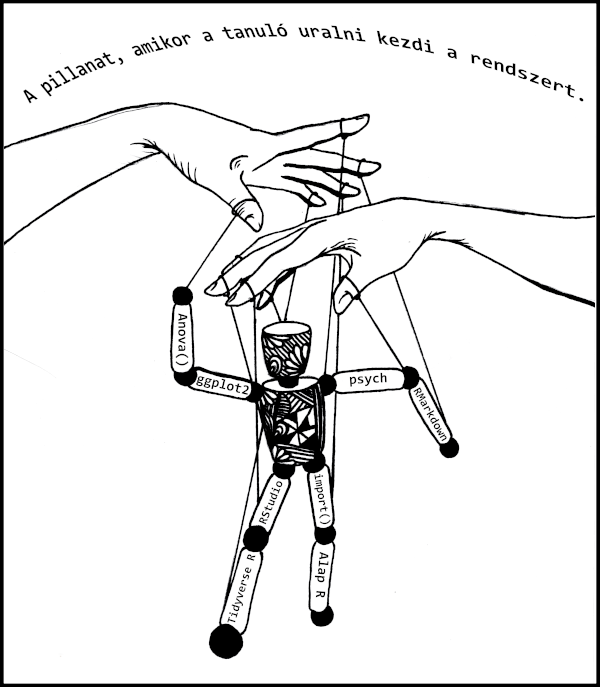
\includegraphics[width=0.7\linewidth]{images/ch_11_small} \end{center}

\hypertarget{reprodukuxe1lhatuxf3-kutatuxe1s}{%
\section{Reprodukálható kutatás}\label{reprodukuxe1lhatuxf3-kutatuxe1s}}

A kutatás és oktatás világában jelentős elmozdulás figyelhető meg a reprodukálható kutatás felé.

igénye felé. „Az akadémiai kutatás végső terméke a papír, a laboratóriumi jegyzetfüzetekkel és a teljes számítási környezettel együtt az eredmények előállítása érdekében, mint például a kód, az adatok stb., Amelyek felhasználhatók az eredmények reprodukálására és új munka létrehozására a kutatás ''(Wikipedia).

Ennek következménye az, hogy meg kell változtatnunk szokásainkat, és minden kéziratunkat, előadásainkat, házi feladatainkat stb. Tiszta és reprodukálható formában kell elkezdenünk, azaz ha valaki megadja a kódot, akkor ez a személy pontosan reprodukálhatja a dokumentumot. Ez a dokumentum megkönnyíti ezt az átmenetet az R Markdown segítségével.

\hypertarget{oravazlat-az-r-tanitasahoz}{%
\chapter{Óravázlat az R tanításához}\label{oravazlat-az-r-tanitasahoz}}

Az R oktatásához és tanulásához egy lehetséges tanmenet vázlatát
mutatjuk be. Az R tanulmányozását két féléves rendszerben, félévenként
10 duplaórában képzeltük el. A lent felsorolt óravázlat összesen 20
duplaórában sorolja fel azokat az ismeretelemeket, amelyek az R
gyakorlati felhasználásához nem nélkülözhetők.

\hypertarget{felev-1}{%
\section*{1. félév}\label{felev-1}}
\addcontentsline{toc}{section}{1. félév}

\textbf{1. óra}\\
Az \emph{Alap R} és az \emph{RStudio} letöltése és telepítése, dokumentációk az
R használatához. Az \emph{RGui} áttekintése, a konzol használata, a
szkriptablak használata, parancsok végrehajtása. Az \emph{RStudio}
használata.

\textbf{2. óra}\\
Számok írása, numerikus operátorok. Karakteres konstansok az R-ben.
Logikai konstansok és a logikai műveletek. Objektum létrehozása, értékének megváltoztatása. Objektumokat is tartalmazó kifejezések.

\textbf{3. óra}\\
Függvények hívása, például a \texttt{log()} és \texttt{exp()} függvények bemutatása, egyéb matematikai függvények. Függvényparaméterek elnevezése, sorrendjük cseréje. Kifejezés definíciója. Vektor adatszerkezet definíciója. Vektor létrehozása: \texttt{c()}, \texttt{:} (kettőspont operátor), \texttt{seq()}, \texttt{rep()}

\textbf{4. óra}\\
A faktor adatszerkezet definíciója, faktor létrehozása a \texttt{factor()} függvénnyel. Objektumok adattípusának megtekintése és az objektum hossza: \texttt{class()}, \texttt{typeof()}, \texttt{length()}. Adattábla definíciója, létrehozása a \texttt{data.frame()} függvénnyel. Mátrix adatszerkezet, létrehozása a \texttt{matrix()} függvénnyel. Tömb adatszerkezet, létrehozása az \texttt{array()} függvénnyel. Lista adatszerkezet, létrehozása a \texttt{list()} függvénnyel. Indexelés vektor, mátrix, tömb és adattábla esetén. Hivatkozás listaelemekre lista és adattábla esetén.

\textbf{5. óra}\\
Tagolt szöveges állomány létrehozása táblázatkezelővel és szövegszerkesztővel. Tagolt szöveges állomány beolvasása a \texttt{read.table()} függvénnyel. A paraméterek megbeszélése (\texttt{file=}, \texttt{sep=}, \texttt{header=}, \texttt{dec=}, \texttt{quote=}, \texttt{stringsAsFactors=}, \texttt{comment.char=}, \texttt{na.strings=}, \texttt{strip.white=}, \texttt{fileEncode=}). Táblázatkezelők és más statisztikai programcsomagok saját formátomú állományainak beolvasása a \texttt{rio::import()} segítségével. A beolvasás helyességének ellenőrzése az \texttt{str()} függvénnyel A \texttt{read.table()} argumentumainak hatása az \texttt{str()} outputjára. Adatállomány kiírása a \texttt{write.table()} és a \texttt{rio::export()} segítségével.

\textbf{6. óra}\\
Egyszerű típuskonverziók (numerikus vektorból faktor és karakteres vektorból faktor előállítása a \texttt{factor()} függvénnyel, valamint az \texttt{as.character()} és \texttt{as.numeric()} használata). Kapcsolat a statisztikai skálák és a változók típusai között. Faktor szintjeinek átnevezése, a szintek sorrendjének meghatározása. Vektor rendezése a \texttt{sort()} és \texttt{order()} függvénnyel. Adattábla rendezése az \texttt{order()} függvénnyel. Adattábla szűrése egyszerű logikai kifejezéssel és összetett logikai kifejezéssel.

\textbf{7. óra}\\
Az R környezet fogalmai: munkakönyvtár, munkaterület, csomag. Munkakönyvtár kezelése Objektum létrehozása és eltávolítása a munkaterületről, objektumok listája. Csomag telepítése, telepített csomagok listája, csomag betöltése, csomag eltávolítása, betöltött csomagok listája. Az R Commander telepítése és használatának bemutatása. A jamovi telepítése és használata. Az RGUI, RStudio, jamovi és az R Commander összehasonlítása.

\textbf{8. óra}\\
Leíró statisztikai mérőszámok meghatározása: \texttt{summary()}, \texttt{mean()}, \texttt{median()}, \texttt{sd()} stb. Hiányzó értékek kezelése (\texttt{na.rm=T}, \texttt{is.na()}, \texttt{na.ommit()}). Műveletek több változóra és csoportra (\texttt{apply()}, \texttt{sapply()}, \texttt{tapply()}, \texttt{aggregate()}, \texttt{by()}). A \texttt{psych::describe()}, \texttt{psych::describeBy()} és a \texttt{DescTools::Desc()} függvényének bemutatása.

\textbf{9. óra}\\
Gyakorisági táblázatok létrehozása a \texttt{table()} és \texttt{xtabs()} függvénnyel. Hiányzó értékek kezelése (\texttt{useNA="ifany"}). Relatív gyakorisági táblázatok. Kumulált gyakorisági táblázatok. Soronként vagy oszloponként vett kétdimenziós gyakorisági táblázatok. Három vagy többdimenziós táblázatok (\texttt{array()} és \texttt{ftable()}). Gyakorisági táblázatok a \texttt{DescTools::Desc()} függvénnyel.

\textbf{10. óra}\\
A hagyományos grafika magasszintű függvényei. Oszlopdiagram rajzolása (\texttt{barplot()}). Egydimenziós pontdiagram létrehozása (\texttt{stripchart()}). Grafikus paraméterek fogalma és beállítása a \texttt{par()} függvénnyel. Feliratok (\texttt{main=}, \texttt{sub=}, \texttt{xlab=}, \texttt{ylab=}, \texttt{las=}), tengelyek (\texttt{xlim=}, \texttt{ylim=}, \texttt{mgp=}, \texttt{tcl=}), pontkarakterek (\texttt{pch=}), margók (\texttt{mar=}), színek (\texttt{col=}) beállítása. Pontdiagram és vonaldiagram rajzolása (\texttt{plot()}). Dobozdiagram rajzolása (\texttt{boxplot()}). Hisztogram rajzolása (\texttt{hist()}). További grafikus paraméterek: rajzterület felosztása (\texttt{mfrow=}, \texttt{mfcol=}). Grafikus eszközök típusai (\texttt{windows()}, \texttt{png()}, \texttt{jpeg()}, \texttt{pdf()}). Képállományok létrehozása és beállítási lehetőségek (\texttt{res=}, \texttt{width=}, \texttt{height=}). Grafikus eszközök bezárása.

\hypertarget{felev-2}{%
\section*{2. félév}\label{felev-2}}
\addcontentsline{toc}{section}{2. félév}

\textbf{11. óra}\\
A reprodukálható kutatás elvének bemutatása. Az RStudio és a jamovi lehetőségei a reprodukálható kutatásban. RMarkdown állomány (\texttt{*.Rmd}) létrehozása, szintaxisának bemutatása. A fejléc lehetőségei. A szöveges rész formázása Markdown segítségével. Az R csonkok lehetőségei. PDF, Word és HTML állomány generálása. Egyedi template-ek használata.

\textbf{12. óra}\\
Információk az adatobjektumokról (\texttt{str()}, \texttt{head()}, \texttt{dim()}, \texttt{nrow()}, \texttt{ncol()}, \texttt{names()}, \texttt{colnames()}, \texttt{rownames()}, \texttt{levels()}, \texttt{nlevels()}). Egyszerű típuskonverzió a karakters, numerikus, logikai és faktor típusok között (\texttt{factor()}, \texttt{as.factor()}, \texttt{as.numeric()}, \texttt{as.character()}, \texttt{as.logical()}). Mátrix és adattábla sor- és oszlopmanipulációja: sor és oszlopnevek megadása, átnevezése, sorok és oszlopok törlése, beszúrása és cseréje (pl. \texttt{rbind()}, \texttt{cbind()}) Numerikusból numerikus transzformáció (tetszőleges matematikai függvény, \texttt{transform()}, \texttt{recode()}). Numerikusból faktor transzformáció (\texttt{cut()}, \texttt{car::recode()}). Faktorból faktor transzformáció (\texttt{car::recode()}).

\textbf{13. óra}\\
Adatelőkészítés egy- és kétmintás próbákhoz. Adatbázis létrehozás a \texttt{data.frame()} függvénnyel a varianciaelemzés számára (kiegyensúlyozott és nem kiegyensúlyozott esetek). A hosszú és széles adatbázisok fogalma Adatbázis átalakítása a két formátum között (\texttt{reshape()}, \texttt{melt()}, \texttt{dcast()}) Adattáblák összefűzése (\texttt{merge()}).

\textbf{14. óra}\\
Egymintás és kétmintás próbák végrehajtása Argumentumok és outputok értelmezése. Például a \texttt{BSDA::z.test()}, \texttt{t.test()}, \texttt{prop.test()}, \texttt{binom.test()}, \texttt{fisher.test()}, \texttt{mcnemar.test()}, \texttt{wilcox.test()}, \texttt{kruskal.test()} és \texttt{friedman.test()} függvényekkel. A varianciaelemzés különböző változatainak végrehajtása. Argumentumok és outputok értelmezése az \texttt{aov()} és \texttt{lm()} függvények esetében. Korreláció- és regressziószámítás végrehajtása. Argumentumok és outputok értelmezése a \texttt{cor()}, \texttt{cor.test()} és \texttt{lm()} esetében.

\textbf{15. óra}\\
Véletlen a \texttt{sample()} függvény segítségével. Eloszlások függvényei (\texttt{r...()}, \texttt{d...()}, \texttt{q...()}, \texttt{p...()}). Kritikus értékek és p-értékek meghatározása a \texttt{q...()}, \texttt{p...()} függvényekkel. Eloszlások sűrűségfüggvényeinek rajzolása a \texttt{curve()} függvény segítségével.

\textbf{16. óra}\\
A Tidyverse R bemutatása. A pipe operátor (\texttt{\%\textgreater{}\%}) használata. A tibble adatobjektumok kezelése. Adatállományok beolvasás és kiírása. Adatobjektom vizsgálata, sor- és oszlopnevek manipulációja. Oszlopok leválogatása, beszúrása és törlése. Adatobjektum rendezése.

\textbf{17. óra}\\
A Tidyverse R bemutatása. Sorok szűrése, törlése és beszúrása. Adatok összesítése, csoportosítása és transzformációja, valamint adattáblák összefűzése a \textbf{dplyr} csomag segítségével. Kategorikus változók kezelése a \textbf{forcats} csomag segítségével.

\textbf{18. óra}\\
A Tidyverse R bemutatása. Széles-hosszú átalakítás a \textbf{tidyr} csomag segítségével (\texttt{pivot\_wider()}, \texttt{pivot\_longer()}). Hiányzó, duplikált és kiugró értékek kezelése a \textbf{dplyr} csomag segítségével. Karakterláncok kezelése a \textbf{stringr} csomag segítségével.

\textbf{19. óra}\\
A ggplot2 grafikus rendszer elemei: az adat, az alakzat (geom) és a megjelenés (aes) rétegek. Az \texttt{x=}, \texttt{y=}, \texttt{alpha=}, \texttt{colour=}, \texttt{fill=}, \texttt{group=}, \texttt{shape=} és \texttt{size=} paraméterek használata az \texttt{aes()} függvényben. Jelmagyarázat megjelenítése. Több ábra megjelenítése kategorikus változó alapján (faceting). Ábra elemeinek beállítása: feliratok, tengelyek, színek és témák. Ábrák mentése.

\textbf{20. óra}\\
Az alavető ábratípusok megjelenítése és paraméterezései: oszlopdiagram, egydimenziós pontdiagram, hisztogram, dobozdiagram, pontdiagram, vonaldiagram, Q-Q ábra, hegedűdiagram, lollipop ábra és terület diagram.

\textbf{20+1. óra}\\
Az R programozási lehetőségei: szekvencia, feltételes utasítások, ciklusok. Függvények létrehozása. Objektum-orientált lehetőségek.

\hypertarget{probak}{%
\chapter{Próbák röviden}\label{probak}}

A könyvben szereplő próba összes próba bemutatása.

\begin{Shaded}
\begin{Highlighting}[]
\FunctionTok{library}\NormalTok{(tidyverse)}
\FunctionTok{library}\NormalTok{(broom)}
\FunctionTok{library}\NormalTok{(knitr)}
\FunctionTok{library}\NormalTok{(apa)}
\CommentTok{\# install.packages("devtools")}
\CommentTok{\# devtools::install\_github(\textquotesingle{}achetverikov/apastats\textquotesingle{},subdir=\textquotesingle{}apastats\textquotesingle{})}
\FunctionTok{library}\NormalTok{(apastats)}
\CommentTok{\# devtools::install\_github("rempsyc/rempsyc")}
\CommentTok{\# library(rempsyc)}
\CommentTok{\# install.packages("papaja")}
\FunctionTok{library}\NormalTok{(papaja)}
\FunctionTok{library}\NormalTok{(DescTools)}
\FunctionTok{library}\NormalTok{(BSDA)}
\FunctionTok{library}\NormalTok{(nonpar)}
\FunctionTok{library}\NormalTok{(TeachingDemos)}
\FunctionTok{library}\NormalTok{(flextable)}

\FunctionTok{library}\NormalTok{(MASS)}
\FunctionTok{str}\NormalTok{(survey)}
\CommentTok{\#\textgreater{} \textquotesingle{}data.frame\textquotesingle{}:    237 obs. of  12 variables:}
\CommentTok{\#\textgreater{}  $ Sex   : Factor w/ 2 levels "Female","Male": 1 2 2 2 2 1 2 1 2 2 ...}
\CommentTok{\#\textgreater{}  $ Wr.Hnd: num  18.5 19.5 18 18.8 20 18 17.7 17 20 18.5 ...}
\CommentTok{\#\textgreater{}  $ NW.Hnd: num  18 20.5 13.3 18.9 20 17.7 17.7 17.3 19.5 18.5 ...}
\CommentTok{\#\textgreater{}  $ W.Hnd : Factor w/ 2 levels "Left","Right": 2 1 2 2 2 2 2 2 2 2 ...}
\CommentTok{\#\textgreater{}  $ Fold  : Factor w/ 3 levels "L on R","Neither",..: 3 3 1 3 2 1 1 3 3 3 ...}
\CommentTok{\#\textgreater{}  $ Pulse : int  92 104 87 NA 35 64 83 74 72 90 ...}
\CommentTok{\#\textgreater{}  $ Clap  : Factor w/ 3 levels "Left","Neither",..: 1 1 2 2 3 3 3 3 3 3 ...}
\CommentTok{\#\textgreater{}  $ Exer  : Factor w/ 3 levels "Freq","None",..: 3 2 2 2 3 3 1 1 3 3 ...}
\CommentTok{\#\textgreater{}  $ Smoke : Factor w/ 4 levels "Heavy","Never",..: 2 4 3 2 2 2 2 2 2 2 ...}
\CommentTok{\#\textgreater{}  $ Height: num  173 178 NA 160 165 ...}
\CommentTok{\#\textgreater{}  $ M.I   : Factor w/ 2 levels "Imperial","Metric": 2 1 NA 2 2 1 1 2 2 2 ...}
\CommentTok{\#\textgreater{}  $ Age   : num  18.2 17.6 16.9 20.3 23.7 ...}

\FunctionTok{options}\NormalTok{(}\AttributeTok{OutDec=}\StringTok{","}\NormalTok{)}

\CommentTok{\# egymintás u{-}próba}
\NormalTok{test.result }\OtherTok{\textless{}{-}}\NormalTok{ BSDA}\SpecialCharTok{::}\FunctionTok{z.test}\NormalTok{(}\AttributeTok{x =}\NormalTok{ survey}\SpecialCharTok{$}\NormalTok{Wr.Hnd, }\AttributeTok{mu =} \DecValTok{16}\NormalTok{, }\AttributeTok{sigma.x =} \DecValTok{3}\NormalTok{) }
\NormalTok{test.result   }\CommentTok{\# hagyományos R output}
\CommentTok{\#\textgreater{} }
\CommentTok{\#\textgreater{}  One{-}sample z{-}Test}
\CommentTok{\#\textgreater{} }
\CommentTok{\#\textgreater{} data:  survey$Wr.Hnd}
\CommentTok{\#\textgreater{} z = 14, p{-}value \textless{}2e{-}16}
\CommentTok{\#\textgreater{} alternative hypothesis: true mean is not equal to 16}
\CommentTok{\#\textgreater{} 95 percent confidence interval:}
\CommentTok{\#\textgreater{}  18,29 19,05}
\CommentTok{\#\textgreater{} sample estimates:}
\CommentTok{\#\textgreater{} mean of x }
\CommentTok{\#\textgreater{}     18,67}
\NormalTok{test.result }\SpecialCharTok{\%\textgreater{}\%}\NormalTok{ broom}\SpecialCharTok{::}\FunctionTok{tidy}\NormalTok{() }\SpecialCharTok{\%\textgreater{}\%}\NormalTok{ knitr}\SpecialCharTok{::}\FunctionTok{kable}\NormalTok{()}
\end{Highlighting}
\end{Shaded}

\begin{tabular}{r|r|r|r|r|l|l}
\hline
estimate & statistic & p.value & conf.low & conf.high & method & alternative\\
\hline
18,67 & 13,67 & 0 & 18,29 & 19,05 & One-sample z-Test & two.sided\\
\hline
\end{tabular}

\begin{Shaded}
\begin{Highlighting}[]
\NormalTok{test.result }\SpecialCharTok{\%\textgreater{}\%}\NormalTok{ papaja}\SpecialCharTok{::}\FunctionTok{apa\_print}\NormalTok{() }\SpecialCharTok{\%\textgreater{}\%} \StringTok{\textasciigrave{}}\AttributeTok{[[}\StringTok{\textasciigrave{}}\NormalTok{(}\StringTok{"full\_result"}\NormalTok{)}
\CommentTok{\#\textgreater{} [1] "$M = 18,67$, 95\textbackslash{}\textbackslash{}\% CI $[18,29, 19,05]$, $z = 13,67$, $p \textless{} 0,001$"}
\NormalTok{test.result }\SpecialCharTok{\%\textgreater{}\%} \FunctionTok{as\_flextable}\NormalTok{()}
\end{Highlighting}
\end{Shaded}

\providecommand{\docline}[3]{\noalign{\global\setlength{\arrayrulewidth}{#1}}\arrayrulecolor[HTML]{#2}\cline{#3}}

\setlength{\tabcolsep}{2pt}

\renewcommand*{\arraystretch}{1.5}

\begin{longtable}[c]{|p{0.86in}|p{0.79in}|p{0.93in}|p{0.85in}|p{0.91in}|p{1.58in}|p{0.99in}}



\hhline{>{\arrayrulecolor[HTML]{666666}\global\arrayrulewidth=2pt}->{\arrayrulecolor[HTML]{666666}\global\arrayrulewidth=2pt}->{\arrayrulecolor[HTML]{666666}\global\arrayrulewidth=2pt}->{\arrayrulecolor[HTML]{666666}\global\arrayrulewidth=2pt}->{\arrayrulecolor[HTML]{666666}\global\arrayrulewidth=2pt}->{\arrayrulecolor[HTML]{666666}\global\arrayrulewidth=2pt}->{\arrayrulecolor[HTML]{666666}\global\arrayrulewidth=2pt}-}

\multicolumn{1}{!{\color[HTML]{000000}\vrule width 0pt}>{\raggedleft}p{\dimexpr 0.86in+0\tabcolsep+0\arrayrulewidth}}{\fontsize{11}{11}\selectfont{\textcolor[HTML]{000000}{\global\setmainfont{Arial}{estimate}}}} & \multicolumn{1}{!{\color[HTML]{000000}\vrule width 0pt}>{\raggedleft}p{\dimexpr 0.79in+0\tabcolsep+0\arrayrulewidth}}{\fontsize{11}{11}\selectfont{\textcolor[HTML]{000000}{\global\setmainfont{Arial}{statistic}}}} & \multicolumn{1}{!{\color[HTML]{000000}\vrule width 0pt}>{\raggedleft}p{\dimexpr 0.93in+0\tabcolsep+0\arrayrulewidth}}{\fontsize{11}{11}\selectfont{\textcolor[HTML]{000000}{\global\setmainfont{Arial}{p.value}}}} & \multicolumn{1}{!{\color[HTML]{000000}\vrule width 0pt}>{\raggedleft}p{\dimexpr 0.85in+0\tabcolsep+0\arrayrulewidth}}{\fontsize{11}{11}\selectfont{\textcolor[HTML]{000000}{\global\setmainfont{Arial}{conf.low}}}} & \multicolumn{1}{!{\color[HTML]{000000}\vrule width 0pt}>{\raggedleft}p{\dimexpr 0.91in+0\tabcolsep+0\arrayrulewidth}}{\fontsize{11}{11}\selectfont{\textcolor[HTML]{000000}{\global\setmainfont{Arial}{conf.high}}}} & \multicolumn{1}{!{\color[HTML]{000000}\vrule width 0pt}>{\raggedright}p{\dimexpr 1.58in+0\tabcolsep+0\arrayrulewidth}}{\fontsize{11}{11}\selectfont{\textcolor[HTML]{000000}{\global\setmainfont{Arial}{method}}}} & \multicolumn{1}{!{\color[HTML]{000000}\vrule width 0pt}>{\raggedright}p{\dimexpr 0.99in+0\tabcolsep+0\arrayrulewidth}!{\color[HTML]{000000}\vrule width 0pt}}{\fontsize{11}{11}\selectfont{\textcolor[HTML]{000000}{\global\setmainfont{Arial}{alternative}}}} \\

\hhline{>{\arrayrulecolor[HTML]{666666}\global\arrayrulewidth=2pt}->{\arrayrulecolor[HTML]{666666}\global\arrayrulewidth=2pt}->{\arrayrulecolor[HTML]{666666}\global\arrayrulewidth=2pt}->{\arrayrulecolor[HTML]{666666}\global\arrayrulewidth=2pt}->{\arrayrulecolor[HTML]{666666}\global\arrayrulewidth=2pt}->{\arrayrulecolor[HTML]{666666}\global\arrayrulewidth=2pt}->{\arrayrulecolor[HTML]{666666}\global\arrayrulewidth=2pt}-}

\endfirsthead

\hhline{>{\arrayrulecolor[HTML]{666666}\global\arrayrulewidth=2pt}->{\arrayrulecolor[HTML]{666666}\global\arrayrulewidth=2pt}->{\arrayrulecolor[HTML]{666666}\global\arrayrulewidth=2pt}->{\arrayrulecolor[HTML]{666666}\global\arrayrulewidth=2pt}->{\arrayrulecolor[HTML]{666666}\global\arrayrulewidth=2pt}->{\arrayrulecolor[HTML]{666666}\global\arrayrulewidth=2pt}->{\arrayrulecolor[HTML]{666666}\global\arrayrulewidth=2pt}-}

\multicolumn{1}{!{\color[HTML]{000000}\vrule width 0pt}>{\raggedleft}p{\dimexpr 0.86in+0\tabcolsep+0\arrayrulewidth}}{\fontsize{11}{11}\selectfont{\textcolor[HTML]{000000}{\global\setmainfont{Arial}{estimate}}}} & \multicolumn{1}{!{\color[HTML]{000000}\vrule width 0pt}>{\raggedleft}p{\dimexpr 0.79in+0\tabcolsep+0\arrayrulewidth}}{\fontsize{11}{11}\selectfont{\textcolor[HTML]{000000}{\global\setmainfont{Arial}{statistic}}}} & \multicolumn{1}{!{\color[HTML]{000000}\vrule width 0pt}>{\raggedleft}p{\dimexpr 0.93in+0\tabcolsep+0\arrayrulewidth}}{\fontsize{11}{11}\selectfont{\textcolor[HTML]{000000}{\global\setmainfont{Arial}{p.value}}}} & \multicolumn{1}{!{\color[HTML]{000000}\vrule width 0pt}>{\raggedleft}p{\dimexpr 0.85in+0\tabcolsep+0\arrayrulewidth}}{\fontsize{11}{11}\selectfont{\textcolor[HTML]{000000}{\global\setmainfont{Arial}{conf.low}}}} & \multicolumn{1}{!{\color[HTML]{000000}\vrule width 0pt}>{\raggedleft}p{\dimexpr 0.91in+0\tabcolsep+0\arrayrulewidth}}{\fontsize{11}{11}\selectfont{\textcolor[HTML]{000000}{\global\setmainfont{Arial}{conf.high}}}} & \multicolumn{1}{!{\color[HTML]{000000}\vrule width 0pt}>{\raggedright}p{\dimexpr 1.58in+0\tabcolsep+0\arrayrulewidth}}{\fontsize{11}{11}\selectfont{\textcolor[HTML]{000000}{\global\setmainfont{Arial}{method}}}} & \multicolumn{1}{!{\color[HTML]{000000}\vrule width 0pt}>{\raggedright}p{\dimexpr 0.99in+0\tabcolsep+0\arrayrulewidth}!{\color[HTML]{000000}\vrule width 0pt}}{\fontsize{11}{11}\selectfont{\textcolor[HTML]{000000}{\global\setmainfont{Arial}{alternative}}}} \\

\hhline{>{\arrayrulecolor[HTML]{666666}\global\arrayrulewidth=2pt}->{\arrayrulecolor[HTML]{666666}\global\arrayrulewidth=2pt}->{\arrayrulecolor[HTML]{666666}\global\arrayrulewidth=2pt}->{\arrayrulecolor[HTML]{666666}\global\arrayrulewidth=2pt}->{\arrayrulecolor[HTML]{666666}\global\arrayrulewidth=2pt}->{\arrayrulecolor[HTML]{666666}\global\arrayrulewidth=2pt}->{\arrayrulecolor[HTML]{666666}\global\arrayrulewidth=2pt}-}\endhead



\multicolumn{7}{!{\color[HTML]{FFFFFF}\vrule width 0pt}>{\raggedright}p{\dimexpr 6.91in+12\tabcolsep+6\arrayrulewidth}!{\color[HTML]{FFFFFF}\vrule width 0pt}}{\fontsize{11}{11}\selectfont{\textcolor[HTML]{000000}{\global\setmainfont{Arial}{Signif.\ codes:\ 0\ <=\ '***'\ <\ 0.001\ <\ '**'\ <\ 0.01\ <\ '*'\ <\ 0.05}}}} \\

\endfoot



\multicolumn{1}{!{\color[HTML]{000000}\vrule width 0pt}>{\raggedleft}p{\dimexpr 0.86in+0\tabcolsep+0\arrayrulewidth}}{\fontsize{11}{11}\selectfont{\textcolor[HTML]{000000}{\global\setmainfont{Arial}{18.7}}}} & \multicolumn{1}{!{\color[HTML]{000000}\vrule width 0pt}>{\raggedleft}p{\dimexpr 0.79in+0\tabcolsep+0\arrayrulewidth}}{\fontsize{11}{11}\selectfont{\textcolor[HTML]{000000}{\global\setmainfont{Arial}{13.7}}}} & \multicolumn{1}{!{\color[HTML]{000000}\vrule width 0pt}>{\raggedleft}p{\dimexpr 0.93in+0\tabcolsep+0\arrayrulewidth}}{\fontsize{11}{11}\selectfont{\textcolor[HTML]{000000}{\global\setmainfont{Arial}{0.0000}}}\fontsize{11}{11}\selectfont{\textcolor[HTML]{000000}{\global\setmainfont{Arial}{***}}}} & \multicolumn{1}{!{\color[HTML]{000000}\vrule width 0pt}>{\raggedleft}p{\dimexpr 0.85in+0\tabcolsep+0\arrayrulewidth}}{\fontsize{11}{11}\selectfont{\textcolor[HTML]{000000}{\global\setmainfont{Arial}{18.3}}}} & \multicolumn{1}{!{\color[HTML]{000000}\vrule width 0pt}>{\raggedleft}p{\dimexpr 0.91in+0\tabcolsep+0\arrayrulewidth}}{\fontsize{11}{11}\selectfont{\textcolor[HTML]{000000}{\global\setmainfont{Arial}{19.1}}}} & \multicolumn{1}{!{\color[HTML]{000000}\vrule width 0pt}>{\raggedright}p{\dimexpr 1.58in+0\tabcolsep+0\arrayrulewidth}}{\fontsize{11}{11}\selectfont{\textcolor[HTML]{000000}{\global\setmainfont{Arial}{One-sample\ z-Test}}}} & \multicolumn{1}{!{\color[HTML]{000000}\vrule width 0pt}>{\raggedright}p{\dimexpr 0.99in+0\tabcolsep+0\arrayrulewidth}!{\color[HTML]{000000}\vrule width 0pt}}{\fontsize{11}{11}\selectfont{\textcolor[HTML]{000000}{\global\setmainfont{Arial}{two.sided}}}} \\

\hhline{>{\arrayrulecolor[HTML]{666666}\global\arrayrulewidth=2pt}->{\arrayrulecolor[HTML]{666666}\global\arrayrulewidth=2pt}->{\arrayrulecolor[HTML]{666666}\global\arrayrulewidth=2pt}->{\arrayrulecolor[HTML]{666666}\global\arrayrulewidth=2pt}->{\arrayrulecolor[HTML]{666666}\global\arrayrulewidth=2pt}->{\arrayrulecolor[HTML]{666666}\global\arrayrulewidth=2pt}->{\arrayrulecolor[HTML]{666666}\global\arrayrulewidth=2pt}-}



\end{longtable}

\begin{Shaded}
\begin{Highlighting}[]

\CommentTok{\# egymintás t{-}próba}
\NormalTok{test.result }\OtherTok{\textless{}{-}} \FunctionTok{t.test}\NormalTok{(}\AttributeTok{x =}\NormalTok{ survey}\SpecialCharTok{$}\NormalTok{Wr.Hnd, }\AttributeTok{mu =} \DecValTok{16}\NormalTok{)}
\NormalTok{test.result   }\CommentTok{\# hagyományos R output}
\CommentTok{\#\textgreater{} }
\CommentTok{\#\textgreater{}  One Sample t{-}test}
\CommentTok{\#\textgreater{} }
\CommentTok{\#\textgreater{} data:  survey$Wr.Hnd}
\CommentTok{\#\textgreater{} t = 22, df = 235, p{-}value \textless{}2e{-}16}
\CommentTok{\#\textgreater{} alternative hypothesis: true mean is not equal to 16}
\CommentTok{\#\textgreater{} 95 percent confidence interval:}
\CommentTok{\#\textgreater{}  18,43 18,91}
\CommentTok{\#\textgreater{} sample estimates:}
\CommentTok{\#\textgreater{} mean of x }
\CommentTok{\#\textgreater{}     18,67}
\NormalTok{test.result }\SpecialCharTok{\%\textgreater{}\%}\NormalTok{ broom}\SpecialCharTok{::}\FunctionTok{tidy}\NormalTok{() }\SpecialCharTok{\%\textgreater{}\%}\NormalTok{ knitr}\SpecialCharTok{::}\FunctionTok{kable}\NormalTok{()}
\end{Highlighting}
\end{Shaded}

\begin{tabular}{r|r|r|r|r|r|l|l}
\hline
estimate & statistic & p.value & parameter & conf.low & conf.high & method & alternative\\
\hline
18,67 & 21,82 & 0 & 235 & 18,43 & 18,91 & One Sample t-test & two.sided\\
\hline
\end{tabular}

\begin{Shaded}
\begin{Highlighting}[]
\NormalTok{test.result }\SpecialCharTok{\%\textgreater{}\%}\NormalTok{ papaja}\SpecialCharTok{::}\FunctionTok{apa\_print}\NormalTok{() }\SpecialCharTok{\%\textgreater{}\%} \StringTok{\textasciigrave{}}\AttributeTok{[[}\StringTok{\textasciigrave{}}\NormalTok{(}\StringTok{"full\_result"}\NormalTok{)}
\CommentTok{\#\textgreater{} [1] "$M = 18,67$, 95\textbackslash{}\textbackslash{}\% CI $[18,43, 18,91]$, $t(235) = 21,82$, $p \textless{} 0,001$"}
\NormalTok{test.result }\SpecialCharTok{\%\textgreater{}\%} \FunctionTok{as\_flextable}\NormalTok{()}
\end{Highlighting}
\end{Shaded}

\providecommand{\docline}[3]{\noalign{\global\setlength{\arrayrulewidth}{#1}}\arrayrulecolor[HTML]{#2}\cline{#3}}

\setlength{\tabcolsep}{2pt}

\renewcommand*{\arraystretch}{1.5}

\begin{longtable}[c]{|p{0.86in}|p{0.79in}|p{0.93in}|p{0.98in}|p{0.85in}|p{0.91in}|p{1.52in}|p{0.99in}}



\hhline{>{\arrayrulecolor[HTML]{666666}\global\arrayrulewidth=2pt}->{\arrayrulecolor[HTML]{666666}\global\arrayrulewidth=2pt}->{\arrayrulecolor[HTML]{666666}\global\arrayrulewidth=2pt}->{\arrayrulecolor[HTML]{666666}\global\arrayrulewidth=2pt}->{\arrayrulecolor[HTML]{666666}\global\arrayrulewidth=2pt}->{\arrayrulecolor[HTML]{666666}\global\arrayrulewidth=2pt}->{\arrayrulecolor[HTML]{666666}\global\arrayrulewidth=2pt}->{\arrayrulecolor[HTML]{666666}\global\arrayrulewidth=2pt}-}

\multicolumn{1}{!{\color[HTML]{000000}\vrule width 0pt}>{\raggedleft}p{\dimexpr 0.86in+0\tabcolsep+0\arrayrulewidth}}{\fontsize{11}{11}\selectfont{\textcolor[HTML]{000000}{\global\setmainfont{Arial}{estimate}}}} & \multicolumn{1}{!{\color[HTML]{000000}\vrule width 0pt}>{\raggedleft}p{\dimexpr 0.79in+0\tabcolsep+0\arrayrulewidth}}{\fontsize{11}{11}\selectfont{\textcolor[HTML]{000000}{\global\setmainfont{Arial}{statistic}}}} & \multicolumn{1}{!{\color[HTML]{000000}\vrule width 0pt}>{\raggedleft}p{\dimexpr 0.93in+0\tabcolsep+0\arrayrulewidth}}{\fontsize{11}{11}\selectfont{\textcolor[HTML]{000000}{\global\setmainfont{Arial}{p.value}}}} & \multicolumn{1}{!{\color[HTML]{000000}\vrule width 0pt}>{\raggedleft}p{\dimexpr 0.98in+0\tabcolsep+0\arrayrulewidth}}{\fontsize{11}{11}\selectfont{\textcolor[HTML]{000000}{\global\setmainfont{Arial}{parameter}}}} & \multicolumn{1}{!{\color[HTML]{000000}\vrule width 0pt}>{\raggedleft}p{\dimexpr 0.85in+0\tabcolsep+0\arrayrulewidth}}{\fontsize{11}{11}\selectfont{\textcolor[HTML]{000000}{\global\setmainfont{Arial}{conf.low}}}} & \multicolumn{1}{!{\color[HTML]{000000}\vrule width 0pt}>{\raggedleft}p{\dimexpr 0.91in+0\tabcolsep+0\arrayrulewidth}}{\fontsize{11}{11}\selectfont{\textcolor[HTML]{000000}{\global\setmainfont{Arial}{conf.high}}}} & \multicolumn{1}{!{\color[HTML]{000000}\vrule width 0pt}>{\raggedright}p{\dimexpr 1.52in+0\tabcolsep+0\arrayrulewidth}}{\fontsize{11}{11}\selectfont{\textcolor[HTML]{000000}{\global\setmainfont{Arial}{method}}}} & \multicolumn{1}{!{\color[HTML]{000000}\vrule width 0pt}>{\raggedright}p{\dimexpr 0.99in+0\tabcolsep+0\arrayrulewidth}!{\color[HTML]{000000}\vrule width 0pt}}{\fontsize{11}{11}\selectfont{\textcolor[HTML]{000000}{\global\setmainfont{Arial}{alternative}}}} \\

\hhline{>{\arrayrulecolor[HTML]{666666}\global\arrayrulewidth=2pt}->{\arrayrulecolor[HTML]{666666}\global\arrayrulewidth=2pt}->{\arrayrulecolor[HTML]{666666}\global\arrayrulewidth=2pt}->{\arrayrulecolor[HTML]{666666}\global\arrayrulewidth=2pt}->{\arrayrulecolor[HTML]{666666}\global\arrayrulewidth=2pt}->{\arrayrulecolor[HTML]{666666}\global\arrayrulewidth=2pt}->{\arrayrulecolor[HTML]{666666}\global\arrayrulewidth=2pt}->{\arrayrulecolor[HTML]{666666}\global\arrayrulewidth=2pt}-}

\endfirsthead

\hhline{>{\arrayrulecolor[HTML]{666666}\global\arrayrulewidth=2pt}->{\arrayrulecolor[HTML]{666666}\global\arrayrulewidth=2pt}->{\arrayrulecolor[HTML]{666666}\global\arrayrulewidth=2pt}->{\arrayrulecolor[HTML]{666666}\global\arrayrulewidth=2pt}->{\arrayrulecolor[HTML]{666666}\global\arrayrulewidth=2pt}->{\arrayrulecolor[HTML]{666666}\global\arrayrulewidth=2pt}->{\arrayrulecolor[HTML]{666666}\global\arrayrulewidth=2pt}->{\arrayrulecolor[HTML]{666666}\global\arrayrulewidth=2pt}-}

\multicolumn{1}{!{\color[HTML]{000000}\vrule width 0pt}>{\raggedleft}p{\dimexpr 0.86in+0\tabcolsep+0\arrayrulewidth}}{\fontsize{11}{11}\selectfont{\textcolor[HTML]{000000}{\global\setmainfont{Arial}{estimate}}}} & \multicolumn{1}{!{\color[HTML]{000000}\vrule width 0pt}>{\raggedleft}p{\dimexpr 0.79in+0\tabcolsep+0\arrayrulewidth}}{\fontsize{11}{11}\selectfont{\textcolor[HTML]{000000}{\global\setmainfont{Arial}{statistic}}}} & \multicolumn{1}{!{\color[HTML]{000000}\vrule width 0pt}>{\raggedleft}p{\dimexpr 0.93in+0\tabcolsep+0\arrayrulewidth}}{\fontsize{11}{11}\selectfont{\textcolor[HTML]{000000}{\global\setmainfont{Arial}{p.value}}}} & \multicolumn{1}{!{\color[HTML]{000000}\vrule width 0pt}>{\raggedleft}p{\dimexpr 0.98in+0\tabcolsep+0\arrayrulewidth}}{\fontsize{11}{11}\selectfont{\textcolor[HTML]{000000}{\global\setmainfont{Arial}{parameter}}}} & \multicolumn{1}{!{\color[HTML]{000000}\vrule width 0pt}>{\raggedleft}p{\dimexpr 0.85in+0\tabcolsep+0\arrayrulewidth}}{\fontsize{11}{11}\selectfont{\textcolor[HTML]{000000}{\global\setmainfont{Arial}{conf.low}}}} & \multicolumn{1}{!{\color[HTML]{000000}\vrule width 0pt}>{\raggedleft}p{\dimexpr 0.91in+0\tabcolsep+0\arrayrulewidth}}{\fontsize{11}{11}\selectfont{\textcolor[HTML]{000000}{\global\setmainfont{Arial}{conf.high}}}} & \multicolumn{1}{!{\color[HTML]{000000}\vrule width 0pt}>{\raggedright}p{\dimexpr 1.52in+0\tabcolsep+0\arrayrulewidth}}{\fontsize{11}{11}\selectfont{\textcolor[HTML]{000000}{\global\setmainfont{Arial}{method}}}} & \multicolumn{1}{!{\color[HTML]{000000}\vrule width 0pt}>{\raggedright}p{\dimexpr 0.99in+0\tabcolsep+0\arrayrulewidth}!{\color[HTML]{000000}\vrule width 0pt}}{\fontsize{11}{11}\selectfont{\textcolor[HTML]{000000}{\global\setmainfont{Arial}{alternative}}}} \\

\hhline{>{\arrayrulecolor[HTML]{666666}\global\arrayrulewidth=2pt}->{\arrayrulecolor[HTML]{666666}\global\arrayrulewidth=2pt}->{\arrayrulecolor[HTML]{666666}\global\arrayrulewidth=2pt}->{\arrayrulecolor[HTML]{666666}\global\arrayrulewidth=2pt}->{\arrayrulecolor[HTML]{666666}\global\arrayrulewidth=2pt}->{\arrayrulecolor[HTML]{666666}\global\arrayrulewidth=2pt}->{\arrayrulecolor[HTML]{666666}\global\arrayrulewidth=2pt}->{\arrayrulecolor[HTML]{666666}\global\arrayrulewidth=2pt}-}\endhead



\multicolumn{8}{!{\color[HTML]{FFFFFF}\vrule width 0pt}>{\raggedright}p{\dimexpr 7.83in+14\tabcolsep+7\arrayrulewidth}!{\color[HTML]{FFFFFF}\vrule width 0pt}}{\fontsize{11}{11}\selectfont{\textcolor[HTML]{000000}{\global\setmainfont{Arial}{Signif.\ codes:\ 0\ <=\ '***'\ <\ 0.001\ <\ '**'\ <\ 0.01\ <\ '*'\ <\ 0.05}}}} \\

\endfoot



\multicolumn{1}{!{\color[HTML]{000000}\vrule width 0pt}>{\raggedleft}p{\dimexpr 0.86in+0\tabcolsep+0\arrayrulewidth}}{\fontsize{11}{11}\selectfont{\textcolor[HTML]{000000}{\global\setmainfont{Arial}{18.7}}}} & \multicolumn{1}{!{\color[HTML]{000000}\vrule width 0pt}>{\raggedleft}p{\dimexpr 0.79in+0\tabcolsep+0\arrayrulewidth}}{\fontsize{11}{11}\selectfont{\textcolor[HTML]{000000}{\global\setmainfont{Arial}{21.8}}}} & \multicolumn{1}{!{\color[HTML]{000000}\vrule width 0pt}>{\raggedleft}p{\dimexpr 0.93in+0\tabcolsep+0\arrayrulewidth}}{\fontsize{11}{11}\selectfont{\textcolor[HTML]{000000}{\global\setmainfont{Arial}{0.0000}}}\fontsize{11}{11}\selectfont{\textcolor[HTML]{000000}{\global\setmainfont{Arial}{***}}}} & \multicolumn{1}{!{\color[HTML]{000000}\vrule width 0pt}>{\raggedleft}p{\dimexpr 0.98in+0\tabcolsep+0\arrayrulewidth}}{\fontsize{11}{11}\selectfont{\textcolor[HTML]{000000}{\global\setmainfont{Arial}{235.0}}}} & \multicolumn{1}{!{\color[HTML]{000000}\vrule width 0pt}>{\raggedleft}p{\dimexpr 0.85in+0\tabcolsep+0\arrayrulewidth}}{\fontsize{11}{11}\selectfont{\textcolor[HTML]{000000}{\global\setmainfont{Arial}{18.4}}}} & \multicolumn{1}{!{\color[HTML]{000000}\vrule width 0pt}>{\raggedleft}p{\dimexpr 0.91in+0\tabcolsep+0\arrayrulewidth}}{\fontsize{11}{11}\selectfont{\textcolor[HTML]{000000}{\global\setmainfont{Arial}{18.9}}}} & \multicolumn{1}{!{\color[HTML]{000000}\vrule width 0pt}>{\raggedright}p{\dimexpr 1.52in+0\tabcolsep+0\arrayrulewidth}}{\fontsize{11}{11}\selectfont{\textcolor[HTML]{000000}{\global\setmainfont{Arial}{One\ Sample\ t-test}}}} & \multicolumn{1}{!{\color[HTML]{000000}\vrule width 0pt}>{\raggedright}p{\dimexpr 0.99in+0\tabcolsep+0\arrayrulewidth}!{\color[HTML]{000000}\vrule width 0pt}}{\fontsize{11}{11}\selectfont{\textcolor[HTML]{000000}{\global\setmainfont{Arial}{two.sided}}}} \\

\hhline{>{\arrayrulecolor[HTML]{666666}\global\arrayrulewidth=2pt}->{\arrayrulecolor[HTML]{666666}\global\arrayrulewidth=2pt}->{\arrayrulecolor[HTML]{666666}\global\arrayrulewidth=2pt}->{\arrayrulecolor[HTML]{666666}\global\arrayrulewidth=2pt}->{\arrayrulecolor[HTML]{666666}\global\arrayrulewidth=2pt}->{\arrayrulecolor[HTML]{666666}\global\arrayrulewidth=2pt}->{\arrayrulecolor[HTML]{666666}\global\arrayrulewidth=2pt}->{\arrayrulecolor[HTML]{666666}\global\arrayrulewidth=2pt}-}



\end{longtable}

\begin{Shaded}
\begin{Highlighting}[]


\CommentTok{\# előjel{-}próba}
\NormalTok{test.result }\OtherTok{\textless{}{-}}\NormalTok{ DescTools}\SpecialCharTok{::}\FunctionTok{SignTest}\NormalTok{(}\AttributeTok{x =}\NormalTok{ survey}\SpecialCharTok{$}\NormalTok{Pulse, }\AttributeTok{md =} \DecValTok{56}\NormalTok{)}
\NormalTok{test.result   }\CommentTok{\# hagyományos R output}
\CommentTok{\#\textgreater{} }
\CommentTok{\#\textgreater{}  One{-}sample Sign{-}Test}
\CommentTok{\#\textgreater{} }
\CommentTok{\#\textgreater{} data:  survey$Pulse}
\CommentTok{\#\textgreater{} S = 192, number of differences = 192, p{-}value \textless{}2e{-}16}
\CommentTok{\#\textgreater{} alternative hypothesis: true median is not equal to 0}
\CommentTok{\#\textgreater{} 96,4 percent confidence interval:}
\CommentTok{\#\textgreater{}  71 76}
\CommentTok{\#\textgreater{} sample estimates:}
\CommentTok{\#\textgreater{} median of the differences }
\CommentTok{\#\textgreater{}                      72,5}
\NormalTok{test.result }\SpecialCharTok{\%\textgreater{}\%}\NormalTok{ broom}\SpecialCharTok{::}\FunctionTok{tidy}\NormalTok{() }\SpecialCharTok{\%\textgreater{}\%}\NormalTok{ knitr}\SpecialCharTok{::}\FunctionTok{kable}\NormalTok{()}
\end{Highlighting}
\end{Shaded}

\begin{tabular}{r|r|r|r|r|r|l|l}
\hline
estimate & statistic & p.value & parameter & conf.low.lwr.ci & conf.high.upr.ci & method & alternative\\
\hline
72,5 & 192 & 0 & 192 & 71 & 76 & One-sample Sign-Test & two.sided\\
\hline
\end{tabular}

\begin{Shaded}
\begin{Highlighting}[]
\NormalTok{test.result }\SpecialCharTok{\%\textgreater{}\%}\NormalTok{ papaja}\SpecialCharTok{::}\FunctionTok{apa\_print}\NormalTok{() }\SpecialCharTok{\%\textgreater{}\%} \StringTok{\textasciigrave{}}\AttributeTok{[[}\StringTok{\textasciigrave{}}\NormalTok{(}\StringTok{"full\_result"}\NormalTok{)}
\CommentTok{\#\textgreater{} [1] "$S = 192,00$, $p \textless{} 0,001$"}
\NormalTok{test.result }\SpecialCharTok{\%\textgreater{}\%} \FunctionTok{as\_flextable}\NormalTok{()}
\end{Highlighting}
\end{Shaded}

\providecommand{\docline}[3]{\noalign{\global\setlength{\arrayrulewidth}{#1}}\arrayrulecolor[HTML]{#2}\cline{#3}}

\setlength{\tabcolsep}{2pt}

\renewcommand*{\arraystretch}{1.5}

\begin{longtable}[c]{|p{0.86in}|p{0.79in}|p{0.93in}|p{0.98in}|p{1.24in}|p{1.32in}|p{1.81in}|p{0.99in}}



\hhline{>{\arrayrulecolor[HTML]{666666}\global\arrayrulewidth=2pt}->{\arrayrulecolor[HTML]{666666}\global\arrayrulewidth=2pt}->{\arrayrulecolor[HTML]{666666}\global\arrayrulewidth=2pt}->{\arrayrulecolor[HTML]{666666}\global\arrayrulewidth=2pt}->{\arrayrulecolor[HTML]{666666}\global\arrayrulewidth=2pt}->{\arrayrulecolor[HTML]{666666}\global\arrayrulewidth=2pt}->{\arrayrulecolor[HTML]{666666}\global\arrayrulewidth=2pt}->{\arrayrulecolor[HTML]{666666}\global\arrayrulewidth=2pt}-}

\multicolumn{1}{!{\color[HTML]{000000}\vrule width 0pt}>{\raggedleft}p{\dimexpr 0.86in+0\tabcolsep+0\arrayrulewidth}}{\fontsize{11}{11}\selectfont{\textcolor[HTML]{000000}{\global\setmainfont{Arial}{estimate}}}} & \multicolumn{1}{!{\color[HTML]{000000}\vrule width 0pt}>{\raggedleft}p{\dimexpr 0.79in+0\tabcolsep+0\arrayrulewidth}}{\fontsize{11}{11}\selectfont{\textcolor[HTML]{000000}{\global\setmainfont{Arial}{statistic}}}} & \multicolumn{1}{!{\color[HTML]{000000}\vrule width 0pt}>{\raggedleft}p{\dimexpr 0.93in+0\tabcolsep+0\arrayrulewidth}}{\fontsize{11}{11}\selectfont{\textcolor[HTML]{000000}{\global\setmainfont{Arial}{p.value}}}} & \multicolumn{1}{!{\color[HTML]{000000}\vrule width 0pt}>{\raggedleft}p{\dimexpr 0.98in+0\tabcolsep+0\arrayrulewidth}}{\fontsize{11}{11}\selectfont{\textcolor[HTML]{000000}{\global\setmainfont{Arial}{parameter}}}} & \multicolumn{1}{!{\color[HTML]{000000}\vrule width 0pt}>{\raggedleft}p{\dimexpr 1.24in+0\tabcolsep+0\arrayrulewidth}}{\fontsize{11}{11}\selectfont{\textcolor[HTML]{000000}{\global\setmainfont{Arial}{conf.low.lwr.ci}}}} & \multicolumn{1}{!{\color[HTML]{000000}\vrule width 0pt}>{\raggedleft}p{\dimexpr 1.32in+0\tabcolsep+0\arrayrulewidth}}{\fontsize{11}{11}\selectfont{\textcolor[HTML]{000000}{\global\setmainfont{Arial}{conf.high.upr.ci}}}} & \multicolumn{1}{!{\color[HTML]{000000}\vrule width 0pt}>{\raggedright}p{\dimexpr 1.81in+0\tabcolsep+0\arrayrulewidth}}{\fontsize{11}{11}\selectfont{\textcolor[HTML]{000000}{\global\setmainfont{Arial}{method}}}} & \multicolumn{1}{!{\color[HTML]{000000}\vrule width 0pt}>{\raggedright}p{\dimexpr 0.99in+0\tabcolsep+0\arrayrulewidth}!{\color[HTML]{000000}\vrule width 0pt}}{\fontsize{11}{11}\selectfont{\textcolor[HTML]{000000}{\global\setmainfont{Arial}{alternative}}}} \\

\hhline{>{\arrayrulecolor[HTML]{666666}\global\arrayrulewidth=2pt}->{\arrayrulecolor[HTML]{666666}\global\arrayrulewidth=2pt}->{\arrayrulecolor[HTML]{666666}\global\arrayrulewidth=2pt}->{\arrayrulecolor[HTML]{666666}\global\arrayrulewidth=2pt}->{\arrayrulecolor[HTML]{666666}\global\arrayrulewidth=2pt}->{\arrayrulecolor[HTML]{666666}\global\arrayrulewidth=2pt}->{\arrayrulecolor[HTML]{666666}\global\arrayrulewidth=2pt}->{\arrayrulecolor[HTML]{666666}\global\arrayrulewidth=2pt}-}

\endfirsthead

\hhline{>{\arrayrulecolor[HTML]{666666}\global\arrayrulewidth=2pt}->{\arrayrulecolor[HTML]{666666}\global\arrayrulewidth=2pt}->{\arrayrulecolor[HTML]{666666}\global\arrayrulewidth=2pt}->{\arrayrulecolor[HTML]{666666}\global\arrayrulewidth=2pt}->{\arrayrulecolor[HTML]{666666}\global\arrayrulewidth=2pt}->{\arrayrulecolor[HTML]{666666}\global\arrayrulewidth=2pt}->{\arrayrulecolor[HTML]{666666}\global\arrayrulewidth=2pt}->{\arrayrulecolor[HTML]{666666}\global\arrayrulewidth=2pt}-}

\multicolumn{1}{!{\color[HTML]{000000}\vrule width 0pt}>{\raggedleft}p{\dimexpr 0.86in+0\tabcolsep+0\arrayrulewidth}}{\fontsize{11}{11}\selectfont{\textcolor[HTML]{000000}{\global\setmainfont{Arial}{estimate}}}} & \multicolumn{1}{!{\color[HTML]{000000}\vrule width 0pt}>{\raggedleft}p{\dimexpr 0.79in+0\tabcolsep+0\arrayrulewidth}}{\fontsize{11}{11}\selectfont{\textcolor[HTML]{000000}{\global\setmainfont{Arial}{statistic}}}} & \multicolumn{1}{!{\color[HTML]{000000}\vrule width 0pt}>{\raggedleft}p{\dimexpr 0.93in+0\tabcolsep+0\arrayrulewidth}}{\fontsize{11}{11}\selectfont{\textcolor[HTML]{000000}{\global\setmainfont{Arial}{p.value}}}} & \multicolumn{1}{!{\color[HTML]{000000}\vrule width 0pt}>{\raggedleft}p{\dimexpr 0.98in+0\tabcolsep+0\arrayrulewidth}}{\fontsize{11}{11}\selectfont{\textcolor[HTML]{000000}{\global\setmainfont{Arial}{parameter}}}} & \multicolumn{1}{!{\color[HTML]{000000}\vrule width 0pt}>{\raggedleft}p{\dimexpr 1.24in+0\tabcolsep+0\arrayrulewidth}}{\fontsize{11}{11}\selectfont{\textcolor[HTML]{000000}{\global\setmainfont{Arial}{conf.low.lwr.ci}}}} & \multicolumn{1}{!{\color[HTML]{000000}\vrule width 0pt}>{\raggedleft}p{\dimexpr 1.32in+0\tabcolsep+0\arrayrulewidth}}{\fontsize{11}{11}\selectfont{\textcolor[HTML]{000000}{\global\setmainfont{Arial}{conf.high.upr.ci}}}} & \multicolumn{1}{!{\color[HTML]{000000}\vrule width 0pt}>{\raggedright}p{\dimexpr 1.81in+0\tabcolsep+0\arrayrulewidth}}{\fontsize{11}{11}\selectfont{\textcolor[HTML]{000000}{\global\setmainfont{Arial}{method}}}} & \multicolumn{1}{!{\color[HTML]{000000}\vrule width 0pt}>{\raggedright}p{\dimexpr 0.99in+0\tabcolsep+0\arrayrulewidth}!{\color[HTML]{000000}\vrule width 0pt}}{\fontsize{11}{11}\selectfont{\textcolor[HTML]{000000}{\global\setmainfont{Arial}{alternative}}}} \\

\hhline{>{\arrayrulecolor[HTML]{666666}\global\arrayrulewidth=2pt}->{\arrayrulecolor[HTML]{666666}\global\arrayrulewidth=2pt}->{\arrayrulecolor[HTML]{666666}\global\arrayrulewidth=2pt}->{\arrayrulecolor[HTML]{666666}\global\arrayrulewidth=2pt}->{\arrayrulecolor[HTML]{666666}\global\arrayrulewidth=2pt}->{\arrayrulecolor[HTML]{666666}\global\arrayrulewidth=2pt}->{\arrayrulecolor[HTML]{666666}\global\arrayrulewidth=2pt}->{\arrayrulecolor[HTML]{666666}\global\arrayrulewidth=2pt}-}\endhead



\multicolumn{8}{!{\color[HTML]{FFFFFF}\vrule width 0pt}>{\raggedright}p{\dimexpr 8.93in+14\tabcolsep+7\arrayrulewidth}!{\color[HTML]{FFFFFF}\vrule width 0pt}}{\fontsize{11}{11}\selectfont{\textcolor[HTML]{000000}{\global\setmainfont{Arial}{Signif.\ codes:\ 0\ <=\ '***'\ <\ 0.001\ <\ '**'\ <\ 0.01\ <\ '*'\ <\ 0.05}}}} \\

\endfoot



\multicolumn{1}{!{\color[HTML]{000000}\vrule width 0pt}>{\raggedleft}p{\dimexpr 0.86in+0\tabcolsep+0\arrayrulewidth}}{\fontsize{11}{11}\selectfont{\textcolor[HTML]{000000}{\global\setmainfont{Arial}{72.5}}}} & \multicolumn{1}{!{\color[HTML]{000000}\vrule width 0pt}>{\raggedleft}p{\dimexpr 0.79in+0\tabcolsep+0\arrayrulewidth}}{\fontsize{11}{11}\selectfont{\textcolor[HTML]{000000}{\global\setmainfont{Arial}{192.0}}}} & \multicolumn{1}{!{\color[HTML]{000000}\vrule width 0pt}>{\raggedleft}p{\dimexpr 0.93in+0\tabcolsep+0\arrayrulewidth}}{\fontsize{11}{11}\selectfont{\textcolor[HTML]{000000}{\global\setmainfont{Arial}{0.0000}}}\fontsize{11}{11}\selectfont{\textcolor[HTML]{000000}{\global\setmainfont{Arial}{***}}}} & \multicolumn{1}{!{\color[HTML]{000000}\vrule width 0pt}>{\raggedleft}p{\dimexpr 0.98in+0\tabcolsep+0\arrayrulewidth}}{\fontsize{11}{11}\selectfont{\textcolor[HTML]{000000}{\global\setmainfont{Arial}{192.0}}}} & \multicolumn{1}{!{\color[HTML]{000000}\vrule width 0pt}>{\raggedleft}p{\dimexpr 1.24in+0\tabcolsep+0\arrayrulewidth}}{\fontsize{11}{11}\selectfont{\textcolor[HTML]{000000}{\global\setmainfont{Arial}{71.0}}}} & \multicolumn{1}{!{\color[HTML]{000000}\vrule width 0pt}>{\raggedleft}p{\dimexpr 1.32in+0\tabcolsep+0\arrayrulewidth}}{\fontsize{11}{11}\selectfont{\textcolor[HTML]{000000}{\global\setmainfont{Arial}{76.0}}}} & \multicolumn{1}{!{\color[HTML]{000000}\vrule width 0pt}>{\raggedright}p{\dimexpr 1.81in+0\tabcolsep+0\arrayrulewidth}}{\fontsize{11}{11}\selectfont{\textcolor[HTML]{000000}{\global\setmainfont{Arial}{One-sample\ Sign-Test}}}} & \multicolumn{1}{!{\color[HTML]{000000}\vrule width 0pt}>{\raggedright}p{\dimexpr 0.99in+0\tabcolsep+0\arrayrulewidth}!{\color[HTML]{000000}\vrule width 0pt}}{\fontsize{11}{11}\selectfont{\textcolor[HTML]{000000}{\global\setmainfont{Arial}{two.sided}}}} \\

\hhline{>{\arrayrulecolor[HTML]{666666}\global\arrayrulewidth=2pt}->{\arrayrulecolor[HTML]{666666}\global\arrayrulewidth=2pt}->{\arrayrulecolor[HTML]{666666}\global\arrayrulewidth=2pt}->{\arrayrulecolor[HTML]{666666}\global\arrayrulewidth=2pt}->{\arrayrulecolor[HTML]{666666}\global\arrayrulewidth=2pt}->{\arrayrulecolor[HTML]{666666}\global\arrayrulewidth=2pt}->{\arrayrulecolor[HTML]{666666}\global\arrayrulewidth=2pt}->{\arrayrulecolor[HTML]{666666}\global\arrayrulewidth=2pt}-}



\end{longtable}

\begin{Shaded}
\begin{Highlighting}[]

\CommentTok{\# Wilcoxon{-}próba}
\NormalTok{test.result }\OtherTok{\textless{}{-}} \FunctionTok{wilcox.test}\NormalTok{(}\AttributeTok{x =}\NormalTok{ survey}\SpecialCharTok{$}\NormalTok{Pulse, }\AttributeTok{md =} \DecValTok{56}\NormalTok{)}
\NormalTok{test.result   }\CommentTok{\# hagyományos R output}
\CommentTok{\#\textgreater{} }
\CommentTok{\#\textgreater{}  Wilcoxon signed rank test with continuity correction}
\CommentTok{\#\textgreater{} }
\CommentTok{\#\textgreater{} data:  survey$Pulse}
\CommentTok{\#\textgreater{} V = 18528, p{-}value \textless{}2e{-}16}
\CommentTok{\#\textgreater{} alternative hypothesis: true location is not equal to 0}
\NormalTok{test.result }\SpecialCharTok{\%\textgreater{}\%}\NormalTok{ broom}\SpecialCharTok{::}\FunctionTok{tidy}\NormalTok{() }\SpecialCharTok{\%\textgreater{}\%}\NormalTok{ knitr}\SpecialCharTok{::}\FunctionTok{kable}\NormalTok{()}
\end{Highlighting}
\end{Shaded}

\begin{tabular}{r|r|l|l}
\hline
statistic & p.value & method & alternative\\
\hline
18528 & 0 & Wilcoxon signed rank test with continuity correction & two.sided\\
\hline
\end{tabular}

\begin{Shaded}
\begin{Highlighting}[]
\NormalTok{test.result }\SpecialCharTok{\%\textgreater{}\%}\NormalTok{ papaja}\SpecialCharTok{::}\FunctionTok{apa\_print}\NormalTok{() }\SpecialCharTok{\%\textgreater{}\%} \StringTok{\textasciigrave{}}\AttributeTok{[[}\StringTok{\textasciigrave{}}\NormalTok{(}\StringTok{"full\_result"}\NormalTok{)}
\CommentTok{\#\textgreater{} [1] "$V = 18,528,00$, $p \textless{} 0,001$"}
\NormalTok{test.result }\SpecialCharTok{\%\textgreater{}\%} \FunctionTok{as\_flextable}\NormalTok{()}
\end{Highlighting}
\end{Shaded}

\providecommand{\docline}[3]{\noalign{\global\setlength{\arrayrulewidth}{#1}}\arrayrulecolor[HTML]{#2}\cline{#3}}

\setlength{\tabcolsep}{2pt}

\renewcommand*{\arraystretch}{1.5}

\begin{longtable}[c]{|p{0.88in}|p{0.93in}|p{3.74in}|p{0.99in}}



\hhline{>{\arrayrulecolor[HTML]{666666}\global\arrayrulewidth=2pt}->{\arrayrulecolor[HTML]{666666}\global\arrayrulewidth=2pt}->{\arrayrulecolor[HTML]{666666}\global\arrayrulewidth=2pt}->{\arrayrulecolor[HTML]{666666}\global\arrayrulewidth=2pt}-}

\multicolumn{1}{!{\color[HTML]{000000}\vrule width 0pt}>{\raggedleft}p{\dimexpr 0.88in+0\tabcolsep+0\arrayrulewidth}}{\fontsize{11}{11}\selectfont{\textcolor[HTML]{000000}{\global\setmainfont{Arial}{statistic}}}} & \multicolumn{1}{!{\color[HTML]{000000}\vrule width 0pt}>{\raggedleft}p{\dimexpr 0.93in+0\tabcolsep+0\arrayrulewidth}}{\fontsize{11}{11}\selectfont{\textcolor[HTML]{000000}{\global\setmainfont{Arial}{p.value}}}} & \multicolumn{1}{!{\color[HTML]{000000}\vrule width 0pt}>{\raggedright}p{\dimexpr 3.74in+0\tabcolsep+0\arrayrulewidth}}{\fontsize{11}{11}\selectfont{\textcolor[HTML]{000000}{\global\setmainfont{Arial}{method}}}} & \multicolumn{1}{!{\color[HTML]{000000}\vrule width 0pt}>{\raggedright}p{\dimexpr 0.99in+0\tabcolsep+0\arrayrulewidth}!{\color[HTML]{000000}\vrule width 0pt}}{\fontsize{11}{11}\selectfont{\textcolor[HTML]{000000}{\global\setmainfont{Arial}{alternative}}}} \\

\hhline{>{\arrayrulecolor[HTML]{666666}\global\arrayrulewidth=2pt}->{\arrayrulecolor[HTML]{666666}\global\arrayrulewidth=2pt}->{\arrayrulecolor[HTML]{666666}\global\arrayrulewidth=2pt}->{\arrayrulecolor[HTML]{666666}\global\arrayrulewidth=2pt}-}

\endfirsthead

\hhline{>{\arrayrulecolor[HTML]{666666}\global\arrayrulewidth=2pt}->{\arrayrulecolor[HTML]{666666}\global\arrayrulewidth=2pt}->{\arrayrulecolor[HTML]{666666}\global\arrayrulewidth=2pt}->{\arrayrulecolor[HTML]{666666}\global\arrayrulewidth=2pt}-}

\multicolumn{1}{!{\color[HTML]{000000}\vrule width 0pt}>{\raggedleft}p{\dimexpr 0.88in+0\tabcolsep+0\arrayrulewidth}}{\fontsize{11}{11}\selectfont{\textcolor[HTML]{000000}{\global\setmainfont{Arial}{statistic}}}} & \multicolumn{1}{!{\color[HTML]{000000}\vrule width 0pt}>{\raggedleft}p{\dimexpr 0.93in+0\tabcolsep+0\arrayrulewidth}}{\fontsize{11}{11}\selectfont{\textcolor[HTML]{000000}{\global\setmainfont{Arial}{p.value}}}} & \multicolumn{1}{!{\color[HTML]{000000}\vrule width 0pt}>{\raggedright}p{\dimexpr 3.74in+0\tabcolsep+0\arrayrulewidth}}{\fontsize{11}{11}\selectfont{\textcolor[HTML]{000000}{\global\setmainfont{Arial}{method}}}} & \multicolumn{1}{!{\color[HTML]{000000}\vrule width 0pt}>{\raggedright}p{\dimexpr 0.99in+0\tabcolsep+0\arrayrulewidth}!{\color[HTML]{000000}\vrule width 0pt}}{\fontsize{11}{11}\selectfont{\textcolor[HTML]{000000}{\global\setmainfont{Arial}{alternative}}}} \\

\hhline{>{\arrayrulecolor[HTML]{666666}\global\arrayrulewidth=2pt}->{\arrayrulecolor[HTML]{666666}\global\arrayrulewidth=2pt}->{\arrayrulecolor[HTML]{666666}\global\arrayrulewidth=2pt}->{\arrayrulecolor[HTML]{666666}\global\arrayrulewidth=2pt}-}\endhead



\multicolumn{4}{!{\color[HTML]{FFFFFF}\vrule width 0pt}>{\raggedright}p{\dimexpr 6.54in+6\tabcolsep+3\arrayrulewidth}!{\color[HTML]{FFFFFF}\vrule width 0pt}}{\fontsize{11}{11}\selectfont{\textcolor[HTML]{000000}{\global\setmainfont{Arial}{Signif.\ codes:\ 0\ <=\ '***'\ <\ 0.001\ <\ '**'\ <\ 0.01\ <\ '*'\ <\ 0.05}}}} \\

\endfoot



\multicolumn{1}{!{\color[HTML]{000000}\vrule width 0pt}>{\raggedleft}p{\dimexpr 0.88in+0\tabcolsep+0\arrayrulewidth}}{\fontsize{11}{11}\selectfont{\textcolor[HTML]{000000}{\global\setmainfont{Arial}{18,528.0}}}} & \multicolumn{1}{!{\color[HTML]{000000}\vrule width 0pt}>{\raggedleft}p{\dimexpr 0.93in+0\tabcolsep+0\arrayrulewidth}}{\fontsize{11}{11}\selectfont{\textcolor[HTML]{000000}{\global\setmainfont{Arial}{0.0000}}}\fontsize{11}{11}\selectfont{\textcolor[HTML]{000000}{\global\setmainfont{Arial}{***}}}} & \multicolumn{1}{!{\color[HTML]{000000}\vrule width 0pt}>{\raggedright}p{\dimexpr 3.74in+0\tabcolsep+0\arrayrulewidth}}{\fontsize{11}{11}\selectfont{\textcolor[HTML]{000000}{\global\setmainfont{Arial}{Wilcoxon\ signed\ rank\ test\ with\ continuity\ correction}}}} & \multicolumn{1}{!{\color[HTML]{000000}\vrule width 0pt}>{\raggedright}p{\dimexpr 0.99in+0\tabcolsep+0\arrayrulewidth}!{\color[HTML]{000000}\vrule width 0pt}}{\fontsize{11}{11}\selectfont{\textcolor[HTML]{000000}{\global\setmainfont{Arial}{two.sided}}}} \\

\hhline{>{\arrayrulecolor[HTML]{666666}\global\arrayrulewidth=2pt}->{\arrayrulecolor[HTML]{666666}\global\arrayrulewidth=2pt}->{\arrayrulecolor[HTML]{666666}\global\arrayrulewidth=2pt}->{\arrayrulecolor[HTML]{666666}\global\arrayrulewidth=2pt}-}



\end{longtable}

\begin{Shaded}
\begin{Highlighting}[]

\CommentTok{\# Khí{-}négyzet próba az egymintás varianciára}
\NormalTok{test.result }\OtherTok{\textless{}{-}}\NormalTok{ TeachingDemos}\SpecialCharTok{::}\FunctionTok{sigma.test}\NormalTok{(}\AttributeTok{x =}\NormalTok{ survey}\SpecialCharTok{$}\NormalTok{Wr.Hnd, }\AttributeTok{sigma =} \DecValTok{10}\NormalTok{) }
\NormalTok{test.result   }\CommentTok{\# hagyományos R output}
\CommentTok{\#\textgreater{} }
\CommentTok{\#\textgreater{}  One sample Chi{-}squared test for variance}
\CommentTok{\#\textgreater{} }
\CommentTok{\#\textgreater{} data:  survey$Wr.Hnd}
\CommentTok{\#\textgreater{} X{-}squared = NA, df = 236, p{-}value = NA}
\CommentTok{\#\textgreater{} alternative hypothesis: true variance is not equal to 100}
\CommentTok{\#\textgreater{} 95 percent confidence interval:}
\CommentTok{\#\textgreater{}  NA NA}
\CommentTok{\#\textgreater{} sample estimates:}
\CommentTok{\#\textgreater{} var of survey$Wr.Hnd }
\CommentTok{\#\textgreater{}                   NA}
\CommentTok{\# test.result \%\textgreater{}\% broom::tidy() \%\textgreater{}\% knitr::kable()}
\CommentTok{\# test.result \%\textgreater{}\% papaja::apa\_print() \%\textgreater{}\% \textasciigrave{}[[\textasciigrave{}("full\_result")}
\CommentTok{\# test.result \%\textgreater{}\% as\_flextable()}

\NormalTok{test.result }\OtherTok{\textless{}{-}}\NormalTok{ EnvStats}\SpecialCharTok{::}\FunctionTok{varTest}\NormalTok{(}\AttributeTok{x =}\NormalTok{ survey}\SpecialCharTok{$}\NormalTok{Wr.Hnd, }\AttributeTok{sigma.squared =} \DecValTok{100}\NormalTok{)}
\NormalTok{test.result}
\CommentTok{\#\textgreater{} $statistic}
\CommentTok{\#\textgreater{} Chi{-}Squared }
\CommentTok{\#\textgreater{}       8,297 }
\CommentTok{\#\textgreater{} }
\CommentTok{\#\textgreater{} $parameters}
\CommentTok{\#\textgreater{}  df }
\CommentTok{\#\textgreater{} 235 }
\CommentTok{\#\textgreater{} }
\CommentTok{\#\textgreater{} $p.value}
\CommentTok{\#\textgreater{} [1] 3,033e{-}123}
\CommentTok{\#\textgreater{} }
\CommentTok{\#\textgreater{} $estimate}
\CommentTok{\#\textgreater{} variance }
\CommentTok{\#\textgreater{}    3,531 }
\CommentTok{\#\textgreater{} }
\CommentTok{\#\textgreater{} $null.value}
\CommentTok{\#\textgreater{} variance }
\CommentTok{\#\textgreater{}      100 }
\CommentTok{\#\textgreater{} }
\CommentTok{\#\textgreater{} $alternative}
\CommentTok{\#\textgreater{} [1] "two.sided"}
\CommentTok{\#\textgreater{} }
\CommentTok{\#\textgreater{} $method}
\CommentTok{\#\textgreater{} [1] "Chi{-}Squared Test on Variance"}
\CommentTok{\#\textgreater{} }
\CommentTok{\#\textgreater{} $data.name}
\CommentTok{\#\textgreater{} [1] "survey$Wr.Hnd"}
\CommentTok{\#\textgreater{} }
\CommentTok{\#\textgreater{} $conf.int}
\CommentTok{\#\textgreater{}   LCL   UCL }
\CommentTok{\#\textgreater{} 2,970 4,267 }
\CommentTok{\#\textgreater{} attr(,"conf.level")}
\CommentTok{\#\textgreater{} [1] 0,95}
\CommentTok{\#\textgreater{} }
\CommentTok{\#\textgreater{} attr(,"class")}
\CommentTok{\#\textgreater{} [1] "htestEnvStats"}
\CommentTok{\# test.result \%\textgreater{}\% broom::tidy() \%\textgreater{}\% knitr::kable()}
\CommentTok{\# test.result \%\textgreater{}\% papaja::apa\_print() \%\textgreater{}\% \textasciigrave{}[[\textasciigrave{}("full\_result")}
\CommentTok{\# test.result \%\textgreater{}\% as\_flextable()}


\CommentTok{\# Khí{-}négyzet próba a valószínűségre}
\NormalTok{test.result }\OtherTok{\textless{}{-}}\NormalTok{ TeachingDemos}\SpecialCharTok{::}\FunctionTok{sigma.test}\NormalTok{(}\AttributeTok{x =}\NormalTok{ survey}\SpecialCharTok{$}\NormalTok{Wr.Hnd, }\AttributeTok{sigma =} \DecValTok{10}\NormalTok{) }
\NormalTok{test.result   }\CommentTok{\# hagyományos R output}
\CommentTok{\#\textgreater{} }
\CommentTok{\#\textgreater{}  One sample Chi{-}squared test for variance}
\CommentTok{\#\textgreater{} }
\CommentTok{\#\textgreater{} data:  survey$Wr.Hnd}
\CommentTok{\#\textgreater{} X{-}squared = NA, df = 236, p{-}value = NA}
\CommentTok{\#\textgreater{} alternative hypothesis: true variance is not equal to 100}
\CommentTok{\#\textgreater{} 95 percent confidence interval:}
\CommentTok{\#\textgreater{}  NA NA}
\CommentTok{\#\textgreater{} sample estimates:}
\CommentTok{\#\textgreater{} var of survey$Wr.Hnd }
\CommentTok{\#\textgreater{}                   NA}
\CommentTok{\# test.result \%\textgreater{}\% broom::tidy() \%\textgreater{}\% knitr::kable()}
\CommentTok{\# test.result \%\textgreater{}\% papaja::apa\_print() \%\textgreater{}\% \textasciigrave{}[[\textasciigrave{}("full\_result")}


\CommentTok{\# Shapiro{-}Wilk{-}próba}
\NormalTok{test.result }\OtherTok{\textless{}{-}} \FunctionTok{shapiro.test}\NormalTok{(}\AttributeTok{x =}\NormalTok{ survey}\SpecialCharTok{$}\NormalTok{Pulse)}
\NormalTok{test.result   }\CommentTok{\# hagyományos R output}
\CommentTok{\#\textgreater{} }
\CommentTok{\#\textgreater{}  Shapiro{-}Wilk normality test}
\CommentTok{\#\textgreater{} }
\CommentTok{\#\textgreater{} data:  survey$Pulse}
\CommentTok{\#\textgreater{} W = 0,99, p{-}value = 0,09}
\NormalTok{test.result }\SpecialCharTok{\%\textgreater{}\%}\NormalTok{ broom}\SpecialCharTok{::}\FunctionTok{tidy}\NormalTok{() }\SpecialCharTok{\%\textgreater{}\%}\NormalTok{ knitr}\SpecialCharTok{::}\FunctionTok{kable}\NormalTok{()}
\end{Highlighting}
\end{Shaded}

\begin{tabular}{r|r|l}
\hline
statistic & p.value & method\\
\hline
0,9874 & 0,0863 & Shapiro-Wilk normality test\\
\hline
\end{tabular}

\begin{Shaded}
\begin{Highlighting}[]
\NormalTok{test.result }\SpecialCharTok{\%\textgreater{}\%}\NormalTok{ papaja}\SpecialCharTok{::}\FunctionTok{apa\_print}\NormalTok{() }\SpecialCharTok{\%\textgreater{}\%} \StringTok{\textasciigrave{}}\AttributeTok{[[}\StringTok{\textasciigrave{}}\NormalTok{(}\StringTok{"full\_result"}\NormalTok{)}
\CommentTok{\#\textgreater{} [1] "$W = 0,99$, $p = 0,086$"}
\NormalTok{test.result }\SpecialCharTok{\%\textgreater{}\%} \FunctionTok{as\_flextable}\NormalTok{()}
\end{Highlighting}
\end{Shaded}

\providecommand{\docline}[3]{\noalign{\global\setlength{\arrayrulewidth}{#1}}\arrayrulecolor[HTML]{#2}\cline{#3}}

\setlength{\tabcolsep}{2pt}

\renewcommand*{\arraystretch}{1.5}

\begin{longtable}[c]{|p{0.79in}|p{0.88in}|p{2.10in}}



\hhline{>{\arrayrulecolor[HTML]{666666}\global\arrayrulewidth=2pt}->{\arrayrulecolor[HTML]{666666}\global\arrayrulewidth=2pt}->{\arrayrulecolor[HTML]{666666}\global\arrayrulewidth=2pt}-}

\multicolumn{1}{!{\color[HTML]{000000}\vrule width 0pt}>{\raggedleft}p{\dimexpr 0.79in+0\tabcolsep+0\arrayrulewidth}}{\fontsize{11}{11}\selectfont{\textcolor[HTML]{000000}{\global\setmainfont{Arial}{statistic}}}} & \multicolumn{1}{!{\color[HTML]{000000}\vrule width 0pt}>{\raggedleft}p{\dimexpr 0.88in+0\tabcolsep+0\arrayrulewidth}}{\fontsize{11}{11}\selectfont{\textcolor[HTML]{000000}{\global\setmainfont{Arial}{p.value}}}} & \multicolumn{1}{!{\color[HTML]{000000}\vrule width 0pt}>{\raggedright}p{\dimexpr 2.1in+0\tabcolsep+0\arrayrulewidth}!{\color[HTML]{000000}\vrule width 0pt}}{\fontsize{11}{11}\selectfont{\textcolor[HTML]{000000}{\global\setmainfont{Arial}{method}}}} \\

\hhline{>{\arrayrulecolor[HTML]{666666}\global\arrayrulewidth=2pt}->{\arrayrulecolor[HTML]{666666}\global\arrayrulewidth=2pt}->{\arrayrulecolor[HTML]{666666}\global\arrayrulewidth=2pt}-}

\endfirsthead

\hhline{>{\arrayrulecolor[HTML]{666666}\global\arrayrulewidth=2pt}->{\arrayrulecolor[HTML]{666666}\global\arrayrulewidth=2pt}->{\arrayrulecolor[HTML]{666666}\global\arrayrulewidth=2pt}-}

\multicolumn{1}{!{\color[HTML]{000000}\vrule width 0pt}>{\raggedleft}p{\dimexpr 0.79in+0\tabcolsep+0\arrayrulewidth}}{\fontsize{11}{11}\selectfont{\textcolor[HTML]{000000}{\global\setmainfont{Arial}{statistic}}}} & \multicolumn{1}{!{\color[HTML]{000000}\vrule width 0pt}>{\raggedleft}p{\dimexpr 0.88in+0\tabcolsep+0\arrayrulewidth}}{\fontsize{11}{11}\selectfont{\textcolor[HTML]{000000}{\global\setmainfont{Arial}{p.value}}}} & \multicolumn{1}{!{\color[HTML]{000000}\vrule width 0pt}>{\raggedright}p{\dimexpr 2.1in+0\tabcolsep+0\arrayrulewidth}!{\color[HTML]{000000}\vrule width 0pt}}{\fontsize{11}{11}\selectfont{\textcolor[HTML]{000000}{\global\setmainfont{Arial}{method}}}} \\

\hhline{>{\arrayrulecolor[HTML]{666666}\global\arrayrulewidth=2pt}->{\arrayrulecolor[HTML]{666666}\global\arrayrulewidth=2pt}->{\arrayrulecolor[HTML]{666666}\global\arrayrulewidth=2pt}-}\endhead



\multicolumn{3}{!{\color[HTML]{FFFFFF}\vrule width 0pt}>{\raggedright}p{\dimexpr 3.78in+4\tabcolsep+2\arrayrulewidth}!{\color[HTML]{FFFFFF}\vrule width 0pt}}{\fontsize{11}{11}\selectfont{\textcolor[HTML]{000000}{\global\setmainfont{Arial}{Signif.\ codes:\ 0\ <=\ '***'\ <\ 0.001\ <\ '**'\ <\ 0.01\ <\ '*'\ <\ 0.05}}}} \\

\endfoot



\multicolumn{1}{!{\color[HTML]{000000}\vrule width 0pt}>{\raggedleft}p{\dimexpr 0.79in+0\tabcolsep+0\arrayrulewidth}}{\fontsize{11}{11}\selectfont{\textcolor[HTML]{000000}{\global\setmainfont{Arial}{1.0}}}} & \multicolumn{1}{!{\color[HTML]{000000}\vrule width 0pt}>{\raggedleft}p{\dimexpr 0.88in+0\tabcolsep+0\arrayrulewidth}}{\fontsize{11}{11}\selectfont{\textcolor[HTML]{000000}{\global\setmainfont{Arial}{0.0863}}}\fontsize{11}{11}\selectfont{\textcolor[HTML]{000000}{\global\setmainfont{Arial}{\ \ .}}}} & \multicolumn{1}{!{\color[HTML]{000000}\vrule width 0pt}>{\raggedright}p{\dimexpr 2.1in+0\tabcolsep+0\arrayrulewidth}!{\color[HTML]{000000}\vrule width 0pt}}{\fontsize{11}{11}\selectfont{\textcolor[HTML]{000000}{\global\setmainfont{Arial}{Shapiro-Wilk\ normality\ test}}}} \\

\hhline{>{\arrayrulecolor[HTML]{666666}\global\arrayrulewidth=2pt}->{\arrayrulecolor[HTML]{666666}\global\arrayrulewidth=2pt}->{\arrayrulecolor[HTML]{666666}\global\arrayrulewidth=2pt}-}



\end{longtable}

\begin{Shaded}
\begin{Highlighting}[]


\CommentTok{\# Kolmogorov{-}Szmirnov{-}próba}
\NormalTok{test.result }\OtherTok{\textless{}{-}}\NormalTok{ DescTools}\SpecialCharTok{::}\FunctionTok{LillieTest}\NormalTok{(}\AttributeTok{x =}\NormalTok{ survey}\SpecialCharTok{$}\NormalTok{Pulse)}
\NormalTok{test.result   }\CommentTok{\# hagyományos R output}
\CommentTok{\#\textgreater{} }
\CommentTok{\#\textgreater{}  Lilliefors (Kolmogorov{-}Smirnov) normality test}
\CommentTok{\#\textgreater{} }
\CommentTok{\#\textgreater{} data:  survey$Pulse}
\CommentTok{\#\textgreater{} D = 0,073, p{-}value = 0,01}
\NormalTok{test.result }\SpecialCharTok{\%\textgreater{}\%}\NormalTok{ broom}\SpecialCharTok{::}\FunctionTok{tidy}\NormalTok{() }\SpecialCharTok{\%\textgreater{}\%}\NormalTok{ knitr}\SpecialCharTok{::}\FunctionTok{kable}\NormalTok{()}
\end{Highlighting}
\end{Shaded}

\begin{tabular}{r|r|l}
\hline
statistic & p.value & method\\
\hline
0,073 & 0,0145 & Lilliefors (Kolmogorov-Smirnov) normality test\\
\hline
\end{tabular}

\begin{Shaded}
\begin{Highlighting}[]
\CommentTok{\# test.result \%\textgreater{}\% papaja::apa\_print() \%\textgreater{}\% \textasciigrave{}[[\textasciigrave{}("full\_result")}
\NormalTok{test.result }\SpecialCharTok{\%\textgreater{}\%} \FunctionTok{as\_flextable}\NormalTok{()}
\end{Highlighting}
\end{Shaded}

\providecommand{\docline}[3]{\noalign{\global\setlength{\arrayrulewidth}{#1}}\arrayrulecolor[HTML]{#2}\cline{#3}}

\setlength{\tabcolsep}{2pt}

\renewcommand*{\arraystretch}{1.5}

\begin{longtable}[c]{|p{0.79in}|p{0.90in}|p{3.37in}}



\hhline{>{\arrayrulecolor[HTML]{666666}\global\arrayrulewidth=2pt}->{\arrayrulecolor[HTML]{666666}\global\arrayrulewidth=2pt}->{\arrayrulecolor[HTML]{666666}\global\arrayrulewidth=2pt}-}

\multicolumn{1}{!{\color[HTML]{000000}\vrule width 0pt}>{\raggedleft}p{\dimexpr 0.79in+0\tabcolsep+0\arrayrulewidth}}{\fontsize{11}{11}\selectfont{\textcolor[HTML]{000000}{\global\setmainfont{Arial}{statistic}}}} & \multicolumn{1}{!{\color[HTML]{000000}\vrule width 0pt}>{\raggedleft}p{\dimexpr 0.9in+0\tabcolsep+0\arrayrulewidth}}{\fontsize{11}{11}\selectfont{\textcolor[HTML]{000000}{\global\setmainfont{Arial}{p.value}}}} & \multicolumn{1}{!{\color[HTML]{000000}\vrule width 0pt}>{\raggedright}p{\dimexpr 3.37in+0\tabcolsep+0\arrayrulewidth}!{\color[HTML]{000000}\vrule width 0pt}}{\fontsize{11}{11}\selectfont{\textcolor[HTML]{000000}{\global\setmainfont{Arial}{method}}}} \\

\hhline{>{\arrayrulecolor[HTML]{666666}\global\arrayrulewidth=2pt}->{\arrayrulecolor[HTML]{666666}\global\arrayrulewidth=2pt}->{\arrayrulecolor[HTML]{666666}\global\arrayrulewidth=2pt}-}

\endfirsthead

\hhline{>{\arrayrulecolor[HTML]{666666}\global\arrayrulewidth=2pt}->{\arrayrulecolor[HTML]{666666}\global\arrayrulewidth=2pt}->{\arrayrulecolor[HTML]{666666}\global\arrayrulewidth=2pt}-}

\multicolumn{1}{!{\color[HTML]{000000}\vrule width 0pt}>{\raggedleft}p{\dimexpr 0.79in+0\tabcolsep+0\arrayrulewidth}}{\fontsize{11}{11}\selectfont{\textcolor[HTML]{000000}{\global\setmainfont{Arial}{statistic}}}} & \multicolumn{1}{!{\color[HTML]{000000}\vrule width 0pt}>{\raggedleft}p{\dimexpr 0.9in+0\tabcolsep+0\arrayrulewidth}}{\fontsize{11}{11}\selectfont{\textcolor[HTML]{000000}{\global\setmainfont{Arial}{p.value}}}} & \multicolumn{1}{!{\color[HTML]{000000}\vrule width 0pt}>{\raggedright}p{\dimexpr 3.37in+0\tabcolsep+0\arrayrulewidth}!{\color[HTML]{000000}\vrule width 0pt}}{\fontsize{11}{11}\selectfont{\textcolor[HTML]{000000}{\global\setmainfont{Arial}{method}}}} \\

\hhline{>{\arrayrulecolor[HTML]{666666}\global\arrayrulewidth=2pt}->{\arrayrulecolor[HTML]{666666}\global\arrayrulewidth=2pt}->{\arrayrulecolor[HTML]{666666}\global\arrayrulewidth=2pt}-}\endhead



\multicolumn{3}{!{\color[HTML]{FFFFFF}\vrule width 0pt}>{\raggedright}p{\dimexpr 5.06in+4\tabcolsep+2\arrayrulewidth}!{\color[HTML]{FFFFFF}\vrule width 0pt}}{\fontsize{11}{11}\selectfont{\textcolor[HTML]{000000}{\global\setmainfont{Arial}{Signif.\ codes:\ 0\ <=\ '***'\ <\ 0.001\ <\ '**'\ <\ 0.01\ <\ '*'\ <\ 0.05}}}} \\

\endfoot



\multicolumn{1}{!{\color[HTML]{000000}\vrule width 0pt}>{\raggedleft}p{\dimexpr 0.79in+0\tabcolsep+0\arrayrulewidth}}{\fontsize{11}{11}\selectfont{\textcolor[HTML]{000000}{\global\setmainfont{Arial}{0.1}}}} & \multicolumn{1}{!{\color[HTML]{000000}\vrule width 0pt}>{\raggedleft}p{\dimexpr 0.9in+0\tabcolsep+0\arrayrulewidth}}{\fontsize{11}{11}\selectfont{\textcolor[HTML]{000000}{\global\setmainfont{Arial}{0.0145}}}\fontsize{11}{11}\selectfont{\textcolor[HTML]{000000}{\global\setmainfont{Arial}{\ \ *}}}} & \multicolumn{1}{!{\color[HTML]{000000}\vrule width 0pt}>{\raggedright}p{\dimexpr 3.37in+0\tabcolsep+0\arrayrulewidth}!{\color[HTML]{000000}\vrule width 0pt}}{\fontsize{11}{11}\selectfont{\textcolor[HTML]{000000}{\global\setmainfont{Arial}{Lilliefors\ (Kolmogorov-Smirnov)\ normality\ test}}}} \\

\hhline{>{\arrayrulecolor[HTML]{666666}\global\arrayrulewidth=2pt}->{\arrayrulecolor[HTML]{666666}\global\arrayrulewidth=2pt}->{\arrayrulecolor[HTML]{666666}\global\arrayrulewidth=2pt}-}



\end{longtable}

\begin{Shaded}
\begin{Highlighting}[]

\CommentTok{\# Arány{-}próba}
\NormalTok{test.result }\OtherTok{\textless{}{-}} \FunctionTok{prop.test}\NormalTok{(}\AttributeTok{x =} \DecValTok{61}\NormalTok{, }\AttributeTok{n =} \DecValTok{500}\NormalTok{, }\AttributeTok{p =} \FloatTok{0.108}\NormalTok{)}
\NormalTok{test.result   }\CommentTok{\# hagyományos R output}
\CommentTok{\#\textgreater{} }
\CommentTok{\#\textgreater{}  1{-}sample proportions test with continuity correction}
\CommentTok{\#\textgreater{} }
\CommentTok{\#\textgreater{} data:  61 out of 500, null probability 0.108}
\CommentTok{\#\textgreater{} X{-}squared = 0,88, df = 1, p{-}value = 0,3}
\CommentTok{\#\textgreater{} alternative hypothesis: true p is not equal to 0,108}
\CommentTok{\#\textgreater{} 95 percent confidence interval:}
\CommentTok{\#\textgreater{}  0,09527 0,15470}
\CommentTok{\#\textgreater{} sample estimates:}
\CommentTok{\#\textgreater{}     p }
\CommentTok{\#\textgreater{} 0,122}
\NormalTok{test.result }\SpecialCharTok{\%\textgreater{}\%}\NormalTok{ broom}\SpecialCharTok{::}\FunctionTok{tidy}\NormalTok{() }\SpecialCharTok{\%\textgreater{}\%}\NormalTok{ knitr}\SpecialCharTok{::}\FunctionTok{kable}\NormalTok{()}
\end{Highlighting}
\end{Shaded}

\begin{tabular}{r|r|r|r|r|r|l|l}
\hline
estimate & statistic & p.value & parameter & conf.low & conf.high & method & alternative\\
\hline
0,122 & 0,8771 & 0,349 & 1 & 0,0953 & 0,1547 & 1-sample proportions test with continuity correction & two.sided\\
\hline
\end{tabular}

\begin{Shaded}
\begin{Highlighting}[]
\CommentTok{\# test.result \%\textgreater{}\% papaja::apa\_print() \%\textgreater{}\% \textasciigrave{}[[\textasciigrave{}("full\_result")}

\CommentTok{\# Binomiális{-}próba}
\NormalTok{test.result }\OtherTok{\textless{}{-}} \FunctionTok{binom.test}\NormalTok{(}\AttributeTok{x =} \DecValTok{61}\NormalTok{, }\AttributeTok{n =} \DecValTok{500}\NormalTok{, }\AttributeTok{p =} \FloatTok{0.108}\NormalTok{)}
\NormalTok{test.result   }\CommentTok{\# hagyományos R output}
\CommentTok{\#\textgreater{} }
\CommentTok{\#\textgreater{}  Exact binomial test}
\CommentTok{\#\textgreater{} }
\CommentTok{\#\textgreater{} data:  61 and 500}
\CommentTok{\#\textgreater{} number of successes = 61, number of trials = 500, p{-}value = 0,3}
\CommentTok{\#\textgreater{} alternative hypothesis: true probability of success is not equal to 0,108}
\CommentTok{\#\textgreater{} 95 percent confidence interval:}
\CommentTok{\#\textgreater{}  0,09462 0,15394}
\CommentTok{\#\textgreater{} sample estimates:}
\CommentTok{\#\textgreater{} probability of success }
\CommentTok{\#\textgreater{}                  0,122}
\NormalTok{test.result }\SpecialCharTok{\%\textgreater{}\%}\NormalTok{ broom}\SpecialCharTok{::}\FunctionTok{tidy}\NormalTok{() }\SpecialCharTok{\%\textgreater{}\%}\NormalTok{ knitr}\SpecialCharTok{::}\FunctionTok{kable}\NormalTok{()}
\end{Highlighting}
\end{Shaded}

\begin{tabular}{r|r|r|r|r|r|l|l}
\hline
estimate & statistic & p.value & parameter & conf.low & conf.high & method & alternative\\
\hline
0,122 & 61 & 0,3129 & 500 & 0,0946 & 0,1539 & Exact binomial test & two.sided\\
\hline
\end{tabular}

\begin{Shaded}
\begin{Highlighting}[]
\CommentTok{\# test.result \%\textgreater{}\% papaja::apa\_print() \%\textgreater{}\% \textasciigrave{}[[\textasciigrave{}("full\_result")}



\CommentTok{\# Bartlett{-}próba}
\NormalTok{test.result }\OtherTok{\textless{}{-}} \FunctionTok{bartlett.test}\NormalTok{(Wr.Hnd}\SpecialCharTok{\textasciitilde{}}\NormalTok{Smoke, }\AttributeTok{data=}\NormalTok{survey)}
\NormalTok{test.result   }\CommentTok{\# hagyományos R output}
\CommentTok{\#\textgreater{} }
\CommentTok{\#\textgreater{}  Bartlett test of homogeneity of variances}
\CommentTok{\#\textgreater{} }
\CommentTok{\#\textgreater{} data:  Wr.Hnd by Smoke}
\CommentTok{\#\textgreater{} Bartlett\textquotesingle{}s K{-}squared = 9,8, df = 3, p{-}value = 0,02}
\NormalTok{test.result }\SpecialCharTok{\%\textgreater{}\%}\NormalTok{ broom}\SpecialCharTok{::}\FunctionTok{tidy}\NormalTok{() }\SpecialCharTok{\%\textgreater{}\%}\NormalTok{ knitr}\SpecialCharTok{::}\FunctionTok{kable}\NormalTok{()}
\end{Highlighting}
\end{Shaded}

\begin{tabular}{r|r|r|l}
\hline
statistic & p.value & parameter & method\\
\hline
9,817 & 0,0202 & 3 & Bartlett test of homogeneity of variances\\
\hline
\end{tabular}

\begin{Shaded}
\begin{Highlighting}[]
\NormalTok{test.result }\SpecialCharTok{\%\textgreater{}\%}\NormalTok{ papaja}\SpecialCharTok{::}\FunctionTok{apa\_print}\NormalTok{() }\SpecialCharTok{\%\textgreater{}\%} \StringTok{\textasciigrave{}}\AttributeTok{[[}\StringTok{\textasciigrave{}}\NormalTok{(}\StringTok{"full\_result"}\NormalTok{)}
\CommentTok{\#\textgreater{} [1] "$K\^{}2(3) = 9,82$, $p = 0,020$"}


\CommentTok{\# Levene{-}próba}
\NormalTok{test.result }\OtherTok{\textless{}{-}}\NormalTok{ DescTools}\SpecialCharTok{::}\FunctionTok{LeveneTest}\NormalTok{(Wr.Hnd}\SpecialCharTok{\textasciitilde{}}\NormalTok{Smoke, }\AttributeTok{data=}\NormalTok{survey, }\AttributeTok{center=}\NormalTok{median)}
\NormalTok{test.result   }\CommentTok{\# hagyományos R output}
\CommentTok{\#\textgreater{} Levene\textquotesingle{}s Test for Homogeneity of Variance (center = median)}
\CommentTok{\#\textgreater{}        Df F value Pr(\textgreater{}F)  }
\CommentTok{\#\textgreater{} group   3    3,09  0,028 *}
\CommentTok{\#\textgreater{}       231                 }
\CommentTok{\#\textgreater{} {-}{-}{-}}
\CommentTok{\#\textgreater{} Signif. codes:  0 \textquotesingle{}***\textquotesingle{} 0,001 \textquotesingle{}**\textquotesingle{} 0,01 \textquotesingle{}*\textquotesingle{} 0,05 \textquotesingle{}.\textquotesingle{} 0,1 \textquotesingle{} \textquotesingle{} 1}
\NormalTok{test.result }\SpecialCharTok{\%\textgreater{}\%}\NormalTok{ broom}\SpecialCharTok{::}\FunctionTok{tidy}\NormalTok{() }\SpecialCharTok{\%\textgreater{}\%}\NormalTok{ knitr}\SpecialCharTok{::}\FunctionTok{kable}\NormalTok{()}
\end{Highlighting}
\end{Shaded}

\begin{tabular}{r|r|r|r}
\hline
statistic & p.value & df & df.residual\\
\hline
3,086 & 0,028 & 3 & 231\\
\hline
\end{tabular}

\begin{Shaded}
\begin{Highlighting}[]
\NormalTok{test.result }\SpecialCharTok{\%\textgreater{}\%}\NormalTok{ papaja}\SpecialCharTok{::}\FunctionTok{apa\_print}\NormalTok{() }\SpecialCharTok{\%\textgreater{}\%} \StringTok{\textasciigrave{}}\AttributeTok{[[}\StringTok{\textasciigrave{}}\NormalTok{(}\StringTok{"full\_result"}\NormalTok{)}
\CommentTok{\#\textgreater{} [1] "$F(3, 231) = 3,09$, $p = 0,028$"}


\CommentTok{\# Kruskal{-}Wallis{-}próba}
\NormalTok{test.result }\OtherTok{\textless{}{-}} \FunctionTok{kruskal.test}\NormalTok{(Wr.Hnd}\SpecialCharTok{\textasciitilde{}}\NormalTok{Smoke, }\AttributeTok{data=}\NormalTok{survey)}
\NormalTok{test.result   }\CommentTok{\# hagyományos R output}
\CommentTok{\#\textgreater{} }
\CommentTok{\#\textgreater{}  Kruskal{-}Wallis rank sum test}
\CommentTok{\#\textgreater{} }
\CommentTok{\#\textgreater{} data:  Wr.Hnd by Smoke}
\CommentTok{\#\textgreater{} Kruskal{-}Wallis chi{-}squared = 3,1, df = 3, p{-}value = 0,4}
\NormalTok{test.result }\SpecialCharTok{\%\textgreater{}\%}\NormalTok{ broom}\SpecialCharTok{::}\FunctionTok{tidy}\NormalTok{() }\SpecialCharTok{\%\textgreater{}\%}\NormalTok{ knitr}\SpecialCharTok{::}\FunctionTok{kable}\NormalTok{()}
\end{Highlighting}
\end{Shaded}

\begin{tabular}{r|r|r|l}
\hline
statistic & p.value & parameter & method\\
\hline
3,089 & 0,3781 & 3 & Kruskal-Wallis rank sum test\\
\hline
\end{tabular}

\begin{Shaded}
\begin{Highlighting}[]
\CommentTok{\# test.result \%\textgreater{}\% papaja::apa\_print() \%\textgreater{}\% \textasciigrave{}[[\textasciigrave{}("full\_result")}


\CommentTok{\# Mann{-}Whitney{-}próba}
\NormalTok{test.result }\OtherTok{\textless{}{-}} \FunctionTok{wilcox.test}\NormalTok{(Wr.Hnd}\SpecialCharTok{\textasciitilde{}}\NormalTok{Sex, }\AttributeTok{data=}\NormalTok{survey)}
\NormalTok{test.result   }\CommentTok{\# hagyományos R output}
\CommentTok{\#\textgreater{} }
\CommentTok{\#\textgreater{}  Wilcoxon rank sum test with continuity correction}
\CommentTok{\#\textgreater{} }
\CommentTok{\#\textgreater{} data:  Wr.Hnd by Sex}
\CommentTok{\#\textgreater{} W = 2138, p{-}value \textless{}2e{-}16}
\CommentTok{\#\textgreater{} alternative hypothesis: true location shift is not equal to 0}
\NormalTok{test.result }\SpecialCharTok{\%\textgreater{}\%}\NormalTok{ broom}\SpecialCharTok{::}\FunctionTok{tidy}\NormalTok{() }\SpecialCharTok{\%\textgreater{}\%}\NormalTok{ knitr}\SpecialCharTok{::}\FunctionTok{kable}\NormalTok{()}
\end{Highlighting}
\end{Shaded}

\begin{tabular}{r|r|l|l}
\hline
statistic & p.value & method & alternative\\
\hline
2138 & 0 & Wilcoxon rank sum test with continuity correction & two.sided\\
\hline
\end{tabular}

\begin{Shaded}
\begin{Highlighting}[]
\NormalTok{test.result }\SpecialCharTok{\%\textgreater{}\%}\NormalTok{ papaja}\SpecialCharTok{::}\FunctionTok{apa\_print}\NormalTok{() }\SpecialCharTok{\%\textgreater{}\%} \StringTok{\textasciigrave{}}\AttributeTok{[[}\StringTok{\textasciigrave{}}\NormalTok{(}\StringTok{"full\_result"}\NormalTok{)}
\CommentTok{\#\textgreater{} [1] "$W = 2,137,50$, $p \textless{} 0,001$"}


\CommentTok{\# F{-}próba}
\NormalTok{test.result }\OtherTok{\textless{}{-}} \FunctionTok{var.test}\NormalTok{(Wr.Hnd}\SpecialCharTok{\textasciitilde{}}\NormalTok{Sex, }\AttributeTok{data=}\NormalTok{survey)}
\NormalTok{test.result   }\CommentTok{\# hagyományos R output}
\CommentTok{\#\textgreater{} }
\CommentTok{\#\textgreater{}  F test to compare two variances}
\CommentTok{\#\textgreater{} }
\CommentTok{\#\textgreater{} data:  Wr.Hnd by Sex}
\CommentTok{\#\textgreater{} F = 0,56, num df = 117, denom df = 116, p{-}value = 0,002}
\CommentTok{\#\textgreater{} alternative hypothesis: true ratio of variances is not equal to 1}
\CommentTok{\#\textgreater{} 95 percent confidence interval:}
\CommentTok{\#\textgreater{}  0,3914 0,8122}
\CommentTok{\#\textgreater{} sample estimates:}
\CommentTok{\#\textgreater{} ratio of variances }
\CommentTok{\#\textgreater{}             0,5639}
\NormalTok{test.result }\SpecialCharTok{\%\textgreater{}\%}\NormalTok{ broom}\SpecialCharTok{::}\FunctionTok{tidy}\NormalTok{() }\SpecialCharTok{\%\textgreater{}\%}\NormalTok{ knitr}\SpecialCharTok{::}\FunctionTok{kable}\NormalTok{()}
\end{Highlighting}
\end{Shaded}

\begin{tabular}{r|r|r|r|r|r|r|l|l}
\hline
estimate & num.df & den.df & statistic & p.value & conf.low & conf.high & method & alternative\\
\hline
0,5639 & 117 & 116 & 0,5639 & 0,0022 & 0,3914 & 0,8122 & F test to compare two variances & two.sided\\
\hline
\end{tabular}

\begin{Shaded}
\begin{Highlighting}[]
\NormalTok{test.result }\SpecialCharTok{\%\textgreater{}\%}\NormalTok{ papaja}\SpecialCharTok{::}\FunctionTok{apa\_print}\NormalTok{() }\SpecialCharTok{\%\textgreater{}\%} \StringTok{\textasciigrave{}}\AttributeTok{[[}\StringTok{\textasciigrave{}}\NormalTok{(}\StringTok{"full\_result"}\NormalTok{)}
\CommentTok{\#\textgreater{} [1] "$F(117, 116) = 0,56$, $p = 0,002$"}


\CommentTok{\# kétmintás t{-}próba}
\NormalTok{test.result }\OtherTok{\textless{}{-}} \FunctionTok{t.test}\NormalTok{(Wr.Hnd}\SpecialCharTok{\textasciitilde{}}\NormalTok{Sex, }\AttributeTok{data=}\NormalTok{survey, }\AttributeTok{var.equal=}\NormalTok{T)}
\NormalTok{test.result   }\CommentTok{\# hagyományos R output}
\CommentTok{\#\textgreater{} }
\CommentTok{\#\textgreater{}  Two Sample t{-}test}
\CommentTok{\#\textgreater{} }
\CommentTok{\#\textgreater{} data:  Wr.Hnd by Sex}
\CommentTok{\#\textgreater{} t = {-}11, df = 233, p{-}value \textless{}2e{-}16}
\CommentTok{\#\textgreater{} alternative hypothesis: true difference in means between group Female and group Male is not equal to 0}
\CommentTok{\#\textgreater{} 95 percent confidence interval:}
\CommentTok{\#\textgreater{}  {-}2,544 {-}1,748}
\CommentTok{\#\textgreater{} sample estimates:}
\CommentTok{\#\textgreater{} mean in group Female   mean in group Male }
\CommentTok{\#\textgreater{}                17,60                19,74}
\NormalTok{test.result }\SpecialCharTok{\%\textgreater{}\%}\NormalTok{ broom}\SpecialCharTok{::}\FunctionTok{tidy}\NormalTok{() }\SpecialCharTok{\%\textgreater{}\%}\NormalTok{ knitr}\SpecialCharTok{::}\FunctionTok{kable}\NormalTok{()}
\end{Highlighting}
\end{Shaded}

\begin{tabular}{r|r|r|r|r|r|r|r|l|l}
\hline
estimate & estimate1 & estimate2 & statistic & p.value & parameter & conf.low & conf.high & method & alternative\\
\hline
-2,146 & 17,6 & 19,74 & -10,63 & 0 & 233 & -2,544 & -1,748 & Two Sample t-test & two.sided\\
\hline
\end{tabular}

\begin{Shaded}
\begin{Highlighting}[]
\NormalTok{test.result }\SpecialCharTok{\%\textgreater{}\%}\NormalTok{ papaja}\SpecialCharTok{::}\FunctionTok{apa\_print}\NormalTok{() }\SpecialCharTok{\%\textgreater{}\%} \StringTok{\textasciigrave{}}\AttributeTok{[[}\StringTok{\textasciigrave{}}\NormalTok{(}\StringTok{"full\_result"}\NormalTok{)}
\CommentTok{\#\textgreater{} [1] "$\textbackslash{}\textbackslash{}Delta M = {-}2,15$, 95\textbackslash{}\textbackslash{}\% CI $[{-}2,54, {-}1,75]$, $t(233) = {-}10,63$, $p \textless{} 0,001$"}


\CommentTok{\# AOV}
\NormalTok{test.result }\OtherTok{\textless{}{-}} \FunctionTok{aov}\NormalTok{(Wr.Hnd}\SpecialCharTok{\textasciitilde{}}\NormalTok{Smoke, }\AttributeTok{data=}\NormalTok{survey)}
\FunctionTok{summary}\NormalTok{(test.result)   }\CommentTok{\# hagyományos R output}
\CommentTok{\#\textgreater{}              Df Sum Sq Mean Sq F value Pr(\textgreater{}F)}
\CommentTok{\#\textgreater{} Smoke         3     17    5,51    1,58    0,2}
\CommentTok{\#\textgreater{} Residuals   231    808    3,50               }
\CommentTok{\#\textgreater{} 2 observations deleted due to missingness}
\NormalTok{test.result }\SpecialCharTok{\%\textgreater{}\%}\NormalTok{ broom}\SpecialCharTok{::}\FunctionTok{tidy}\NormalTok{() }\SpecialCharTok{\%\textgreater{}\%}\NormalTok{ knitr}\SpecialCharTok{::}\FunctionTok{kable}\NormalTok{()}
\end{Highlighting}
\end{Shaded}

\begin{tabular}{l|r|r|r|r|r}
\hline
term & df & sumsq & meansq & statistic & p.value\\
\hline
Smoke & 3 & 16,54 & 5,514 & 1,577 & 0,1957\\
\hline
Residuals & 231 & 807,69 & 3,497 & NA & NA\\
\hline
\end{tabular}

\begin{Shaded}
\begin{Highlighting}[]
\NormalTok{test.result }\SpecialCharTok{\%\textgreater{}\%}\NormalTok{ papaja}\SpecialCharTok{::}\FunctionTok{apa\_print}\NormalTok{() }\SpecialCharTok{\%\textgreater{}\%} \StringTok{\textasciigrave{}}\AttributeTok{[[}\StringTok{\textasciigrave{}}\NormalTok{(}\StringTok{"full\_result"}\NormalTok{)}
\CommentTok{\#\textgreater{} $Smoke}
\CommentTok{\#\textgreater{} [1] "$F(3, 231) = 1,58$, $p = 0,196$, $\textbackslash{}\textbackslash{}hat\{\textbackslash{}\textbackslash{}eta\}\^{}2\_G = 0,020$, 90\textbackslash{}\textbackslash{}\% CI $[0,000, 0,049]$"}


\CommentTok{\# AOV {-} Welch}
\NormalTok{test.result }\OtherTok{\textless{}{-}} \FunctionTok{oneway.test}\NormalTok{(Wr.Hnd}\SpecialCharTok{\textasciitilde{}}\NormalTok{Smoke, }\AttributeTok{data=}\NormalTok{survey)}
\NormalTok{test.result   }\CommentTok{\# hagyományos R output}
\CommentTok{\#\textgreater{} }
\CommentTok{\#\textgreater{}  One{-}way analysis of means (not assuming equal variances)}
\CommentTok{\#\textgreater{} }
\CommentTok{\#\textgreater{} data:  Wr.Hnd and Smoke}
\CommentTok{\#\textgreater{} F = 0,89, num df = 3, denom df = 25, p{-}value = 0,5}
\NormalTok{test.result }\SpecialCharTok{\%\textgreater{}\%}\NormalTok{ broom}\SpecialCharTok{::}\FunctionTok{tidy}\NormalTok{() }\SpecialCharTok{\%\textgreater{}\%}\NormalTok{ knitr}\SpecialCharTok{::}\FunctionTok{kable}\NormalTok{()}
\end{Highlighting}
\end{Shaded}

\begin{tabular}{r|r|r|r|l}
\hline
num.df & den.df & statistic & p.value & method\\
\hline
3 & 24,6 & 0,8948 & 0,4578 & One-way analysis of means (not assuming equal variances)\\
\hline
\end{tabular}

\begin{Shaded}
\begin{Highlighting}[]
\NormalTok{test.result }\SpecialCharTok{\%\textgreater{}\%}\NormalTok{ papaja}\SpecialCharTok{::}\FunctionTok{apa\_print}\NormalTok{() }\SpecialCharTok{\%\textgreater{}\%} \StringTok{\textasciigrave{}}\AttributeTok{[[}\StringTok{\textasciigrave{}}\NormalTok{(}\StringTok{"full\_result"}\NormalTok{)}
\CommentTok{\#\textgreater{} [1] "$F(3, 24,60) = 0,89$, $p = 0,458$"}

\CommentTok{\# library(jmv)}
\CommentTok{\# data(\textquotesingle{}ToothGrowth\textquotesingle{})}
\CommentTok{\# ancova(formula = len \textasciitilde{} supp + dose, data = ToothGrowth)}

\CommentTok{\# }
\CommentTok{\# apastats::describe.ttest(t1, show.mean = T)}
\CommentTok{\# }
\CommentTok{\# \# If devtools isn\textquotesingle{}t already installed, install it with install.packages("devtools")}
\CommentTok{\# }
\CommentTok{\# if(!require(\textquotesingle{}pubprint\textquotesingle{})) \{}
\CommentTok{\#   install.packages(\textquotesingle{}pubprint\textquotesingle{})}
\CommentTok{\#   library(\textquotesingle{}pubprint\textquotesingle{})}
\CommentTok{\# \}}
\CommentTok{\# }
\CommentTok{\# }
\CommentTok{\# }
\CommentTok{\# t1 \%\textgreater{}\% tidy() \%\textgreater{}\% kable()}
\CommentTok{\# }
\end{Highlighting}
\end{Shaded}


  \bibliography{bibliography/book.bib}

\end{document}
